% !TEX TS-program = xelatex
% !TEX encoding = UTF-8

% This is a simple template for a XeLaTeX document using the "article" class,
% with the fontspec package to easily select fonts.

\documentclass[oneside,10pt]{book} % use larger type; default would be 10pt

% other LaTeX packages.....

%-------------------------------------------------
% Geometry (et sidenotes) : format tufte light
%-------------------------------------------------

\usepackage{sidenotes}

%\usepackage{mwe}

%\usepackage[showframe]{geometry}
\usepackage{geometry}

% option classique
\geometry{letterpaper, left=2cm, right=3in, top=50pt,bottom=50pt, marginparsep=20pt, marginparwidth=2in,  footskip=40pt}

% Option pour faire un document A5
%\geometry{paperwidth=6in, paperheight=9in, left=2cm, right=2in, top=50pt,bottom=50pt, marginparsep=20pt, marginparwidth=1.5in,  footskip=40pt}
 
\renewcommand{\baselinestretch}{1.1} 
\usepackage{placeins} % floatbarrier
\usepackage{fullwidth}
 
\makeatletter
%\renewcommand{\@sidenotes@adjust}{%
% \checkoddpage%
% \ifoddpage%
% %
% \else%
% %\hspace{\@sidenotes@extrawidth}%    %% this was originally there
% \fi}
%%
%% or
%%
\let\@sidenotes@adjust\relax
\makeatother

\setlength\parindent{0pt}
%\usepackage{marginnote}
%\renewcommand*{\raggedleftmarginnote}{}
%\renewcommand*{\raggedrightmarginnote}{}

% Margin Caption (done with sidenotes package)
% UTILISER \sidecaption pour une caption
%\usepackage[margincaption,rightcaption,ragged,wide]{sidecap}
%\usepackage[margincaption,outercaption]{sidecap}
%\sidecaptionvpos{figure}{t} 
%\sidecaptionvpos{table}{t}
% format des captions des figures
%\captionsetup[SCfigure]{format=plain, ...}
%\captionsetup[SCtable]{format=plain, ...}
%-------------------------------------------------
% cadre
%-------------------------------------------------

\usepackage{tikz}
\usepackage[framemethod=TikZ]{mdframed}
\usetikzlibrary{positioning}  
\usepackage{placeins} % FLoatbarrier to force float

\usepackage{xcolor}
%\hypersetup{colorlinks}% uncomment this line if you prefer colored hyperlinks (e.g., for onscreen viewing)
\usepackage{units}
% Typesets the font size, leading, and measure in the form of 10/12x26 pc.


\newcommand{\measure}[3]{#1/#2$\times$\unit[#3]{pc}}
\newcommand{\coefGraph}{1} % Taille du graphe dans les marges; sert uniquement pour Epub, sinon = 1 x textwidth
%\usepackage{multicol} %multicolum for Definition
\newcommand{\largecoefGraph}{1.2} % Taille du graphe dans les marges en proportion de textwidth; sert uniquement pour Epub, sinon = textwidth; remplacer \textwidth par \coefGraph\textwidth
%\usepackage[table]{xcolor}
%\usepackage[xcdraw]{xcolor}
%\usepackage[dvipsnames]{xcolor}
%\usepackage{amsmath,amssymb,amsthm}
%\usepackage{mathtools}
%\usepackage{mathspec}
%\usepackage{xltxtra,xunicode}
\newcommand{\myinnertopmargin}{0pt} % marge qui sert pour les définitions et proprietés




%-------------------------------------------------
% url
%-------------------------------------------------

\usepackage{blindtext}
\usepackage{hyperref}
\usepackage{url}


%-------------------------------------------------
% tableau
%-------------------------------------------------

% pour mettre des tableaux au bon endroit avec l'option H
%\usepackage{float}
% grands tableaux... pratiques
\usepackage{longtable}
 % pour faire des beaux tableaux
\usepackage{booktabs}

 
%-------------------------------------------------
% caractère
%-------------------------------------------------




\usepackage[sc]{mathpazo}
\linespread{1.05}         % Palladio needs more leading (space between lines)

\usepackage{fontspec} % Font selection for XeLaTeX; see fontspec.pdf for documentation
\defaultfontfeatures{Mapping=tex-text} % to support TeX conventions like ``---''


%\setmainfont{Charis SIL} % set the main body font (\textrm), assumes Charis SIL is installed
%\setsansfont{Deja Vu Sans}
%\setmonofont{Deja Vu Mono}

 % format des fonts comme Tufte
 \usepackage{xunicode} % Unicode support for LaTeX character names (accents, European chars, etc)
\usepackage{xltxtra} % Extra customizations for XeLaTeX
\usepackage{amsmath}
\usepackage{amsthm}
% \usepackage{fontspec}
%\setmainfont[Renderer=Basic, Numbers=OldStyle, Scale = 1.0]{TeX Gyre Pagella}
%\setsansfont[Renderer=Basic, Scale=0.90]{TeX Gyre Heros}
%\setmonofont[Renderer=Basic]{TeX Gyre Cursor}
% Palatino for main text and math
%\usepackage[osf,sc]{mathpazo}

% Helvetica for sans serif
% (scaled to match size of Palatino)
%\usepackage[scaled=0.90]{helvet}

% Bera Mono for monospaced
% (scaled to match size of Palatino)
%\usepackage[scaled=0.85]{beramono}
 
%\setmainfont[Numbers=OldStyle, Scale = 1.0]{TeX Gyre Pagella}
%\setsansfont[Scale=0.90]{TeX Gyre Heros}
%\setmonofont{TeX Gyre Cursor}

% pour le chinois
\usepackage{xeCJK}

%-------------------------------------------------
% caractère
%-------------------------------------------------

%\usepackage{biblatex} %pour citer des numero de page
\usepackage[utf8x]{inputenc}

\usepackage[english,main=french]{babel}



\babelprovide[import]{arabic}
\babelfont[arabic]{rm}{Amiri}
\babelprovide[import]{greek}
\babelfont[greek]{rm}{EB Garamond}
% ex
% \foreignlanguage{greek}{Ἰουδαῖοί τε καὶ προσήλυτο.}
%\babelprovide[import]{greek}
%\babelfont[greek]{rm}[RawFeature=+calt]{SimonciniGaramondPro}
\usepackage{arabtex}
%babel-greek
%\usepackage[sc]{mathpazo}

%\linespread{1.05}         % Palladio needs more leading (space between lines)
%\usepackage[T1]{fontenc}
%\renewcommand{\cftsecfont}{\rmfamily\mdseries\upshape}
%\renewcommand{\cftsecpagefont}{\rmfamily\mdseries\upshape} % No bold!

%TARabe dans Name


%Recherche \hypertarget et remplacer par \vide
% \protect\hyperlink par \vide
%\texorpdfstring par RIEN
% \RL : \TArabe
% rechercher \footnote{ et remplacer par \sn{
% rechercher Al Gazali
% package pour faire des réferences à des labels pour le chapitre théologiens
 
%-------------------------------------------------
% bibliography
%-------------------------------------------------

% 
%\usepackage{natbib}
\usepackage{natbib}
\bibliographystyle{unsrtnat}
\bibliographystyle{kluwer}
%\usepackage[notes,backend=biber]{biblatex-chicago}

%\usepackage[style=reading]{biblatex}
%\usepackage[citestyle=reading,bibstyle=authortitle]{biblatex}

%\addbibresource{Theo.bib}

%\bibliography{sample}
%\bibliography{siam}

%\newcommand*{\sidecite}[1]{\sidenote{[\cite{#1}].\citeauthor{#1} - \citetitle{#1}}



 %--------------------------------------------------------------
% Table des matières
%--------------------------------------------------------------
 \usepackage{titletoc}
%%%%% TABLE OF CONTENTS
\setcounter{tocdepth}{1}

\usepackage{etoc}
%%% ToC (table of contents) APPEARANCE
%\usepackage[nottoc,notlof,notlot]{tocbibind} % Put the bibliography in the ToC
%\usepackage[titles,subfigure]{tocloft} % Alter the style of the Table of Contents

\usepackage{cleveref} % referece



\usepackage{eurosym}  %Euro
\usepackage[super]{nth} %for \nth{1} to give 1st
\usepackage{array} % permet de centrer les tableaux\

% Prints the month name (e.g., January) and the year (e.g., 2008)




%\splittopskip=5cm 

 
%-------------------------------------------------
% édition
%-------------------------------------------------
\usepackage{comment}

%-------------------------------------------------
% multi colonnage
%-------------------------------------------------
\usepackage{multicol}





%--------------------------------------------------------------
% Frame
%--------------------------------------------------------------

\usepackage[framemethod=TikZ]{mdframed}

\usepackage{thmtools}
%\usepackage{amsthm}

\usepackage{blindtext} % avoid to cut theorem
% avoid to have theorem or definition in the list of theorm
\makeatletter
\newcommand{\theosep}{\parsep}
\renewcommand{\theosep}{20pt}


%--------------------------------------------------------------
% Titre des listes de théorèmes
%--------------------------------------------------------------

\renewcommand{\listtheoremname}{List of Important Theorems}

\makeatletter
\def\ll@theorem{%
  \protect\numberline{\csname the\thmt@envname\endcsname}%
  \ifx\@empty\thmt@shortoptarg
    \thmt@thmname
  \else
    \thmt@shortoptarg
  \fi}
\def\l@thmt@theorem{} 
 \makeatother
 

% avoid to have theorem or definition in the list of theorm
\makeatletter
\patchcmd\thmt@mklistcmd
  {\thmt@thmname}
  {\check@optarg{\thmt@thmname}}
  {}{}
\patchcmd\thmt@mklistcmd
  {\thmt@thmname\ifx}
  {\check@optarg{\thmt@thmname}\ifx}
  {}{}
\protected\def\check@optarg#1{%
  \@ifnextchar\thmtformatoptarg\@secondoftwo{#1}%
}

 
\makeatother

% format of theorem


            
\declaretheoremstyle[
    headfont=\scshape, 
    notebraces={\scshape : }{.},
    bodyfont=\normalfont,
    headpunct={},
    postheadspace=\newline,
%    postheadhook={\textcolor{red}{\rule[.6ex]{\linewidth}{0.4pt}}\\},
    spacebelow=\parsep,
    spaceabove=\parsep,
    mdframed={
            backgroundcolor=white!20, 
            splittopskip = \topskip,
            linecolor=blue!30, 
            linewidth = 2pt,
            innertopmargin=\myinnertopmargin,
            roundcorner=1pt, 
            innerbottommargin=6pt, 
            skipabove=\parsep,     
            skipbelow=\parsep} 
    ]{Definitionstyle}
    
\declaretheoremstyle[
    headfont=\scshape, 
    notebraces={\scshape : }{.},
    bodyfont=\normalfont,
    headpunct={},
    postheadspace=\newline,
%    postheadhook={\textcolor{red}{\rule[.6ex]{\linewidth}{0.4pt}}\\},
    spacebelow=\parsep,
    spaceabove=\parsep,
    mdframed={backgroundcolor=white!20, 
            splittopskip = \topskip,
            linecolor=red!30, 
            linewidth = 2pt,
            innertopmargin=\myinnertopmargin,
            roundcorner=1pt, 
            innerbottommargin=6pt, 
            skipabove=\parsep,     
            skipbelow=\parsep} 
    ]{Propertystyle}

%,    postfoothook=
% example environment - thmtools
\declaretheoremstyle[
    headfont=\scshape, 
    notebraces={\scshape : }{.},
    bodyfont=\normalfont,
    headpunct={},
    postheadspace=\newline, 
%    postheadhook={\textcolor{red}{\rule[.6ex]{\linewidth}{0.4pt}}\\},
    spacebelow=\parsep,
    spaceabove=\parsep
]{Exercisestyle}
% example environment - thmtools








\declaretheorem[ style = Exercisestyle, numbered=no,name = Property]{property}
\declaretheorem[ style = Propertystyle, name = {Property} ]{Prop}
\declaretheorem[ style = Propertystyle, name = Theorem, sibling=Prop]{Theo}
\declaretheorem[ style = Propertystyle, name = Theorem, sibling=Prop]{theorem}
\declaretheorem[ style = Propertystyle, name = Lemma, sibling=Prop]{lemma}
\declaretheorem[ style = Exercisestyle, numbered=no,name = {Remark}]{rem}
\declaretheorem[ style = Definitionstyle, name = {Definition}]{definition}
\declaretheorem[ style = Definitionstyle, name = {Definition}, sibling=definition]{Def}
\declaretheorem[ style = Exercisestyle, name = Exercise]{exercise}
\declaretheorem[ style = Exercisestyle, name = Exercise, sibling=exercise]{Exercise}
\declaretheorem[ style = Exercisestyle, name = Exercise, sibling=exercise]{Exc}
\declaretheorem[ style = Exercisestyle, name = Exercise, sibling=exercise]{Exo}
\declaretheorem[ style = Exercisestyle, name = Problem, sibling=exercise]{problem}
\declaretheorem[ style = Exercisestyle, name = Example]{example}
\declaretheorem[ style = Exercisestyle, name = Example, sibling=example]{Ex}
\makeatother


%--------------------------------------------------------------
% Code
%--------------------------------------------------------------

%% Permet de mettre du code
\usepackage{listings}
\lstdefinestyle{mystyle}{
    basicstyle=\ttfamily\footnotesize,
    breakatwhitespace=false,         
    breaklines=true,                 
    captionpos=b,                    
    keepspaces=true,                 
    numbers=left,                    
    numbersep=5pt,                  
    showspaces=false,                
    showstringspaces=false,
    showtabs=false,                  
    tabsize=2
}
\lstset{%
	aboveskip=\topsep,
	belowskip=\topsep,
	xleftmargin=\parindent}

\lstset{style=mystyle}





\newcommand{\bi}{\begin{itemize}}
 \newcommand{\ei}{\end{itemize}}
  \newcommand{\be}{\begin{Ex}}
 \newcommand{\ee}{\end{Ex}}
 \newcommand{\mn}[1]{\marginnote{\footnotesize #1}}
  \newcommand{\sn}[1]{\sidenote{\footnotesize #1}}

\newcommand{\mzt}{\emph{muʿtazilite}}  
\newcommand{\CD}{\emph{la Cité de Dieu }}  

\newcommand{\CB}{\emph{Cedric Baylocq }} % nom du professeur
%Recherche \hypertarget et remplacer par \vide
% \protect\hyperlink par \vide
%\texorpdfstring par RIEN
% \RL : \TArabe
% rechercher \footnote{ et remplacer par \sn{
% rechercher Al Gazali
%\newcommand\TArabe[1]{\foreignlanguage{arabic}{\RL}}
\newcommand\TArabe[1]{\foreignlanguage{arabic}{#1}}
\newcommand{\vide}[1]{}

\renewcommand{\listtheoremname}{Liste des Definitions}

% Prints the month name (e.g., January) and the year (e.g., 2008)
\newcommand{\monthyear}{%
  \ifcase\month\or January\or February\or March\or April\or May\or June\or
  July\or August\or September\or October\or November\or
  December\fi\space\number\year
}

\newcommand{\tnote}{\textsuperscript}


% Inserts a blank page
\newcommand{\blankpage}{\newpage\hbox{}\thispagestyle{empty}\newpage}


% Prints an epigraph and speaker in sans serif, all-caps type.
\newcommand{\openepigraph}[2]{%
  %\sffamily\fontsize{14}{16}\selectfont
  \begin{fullwidth}
  \sffamily\large
  \begin{doublespace}
  \noindent\allcaps{#1}\\% epigraph
  \noindent\allcaps{#2}% author
  \end{doublespace}
  \end{fullwidth}
}
 


 

% Prints argument within hanging parentheses (i.e., parentheses that take
% up no horizontal space).  Useful in tabular environments.
\newcommand{\hangp}[1]{\makebox[0pt][r]{(}#1\makebox[0pt][l]{)}}
\newcommand{\hangstar}{\makebox[0pt][l]{*}}
%%
% Prints an asterisk that takes up no horizontal space.
% Useful in tabular environments.



% Macros for typesetting the documentation
\newcommand{\hlred}[1]{\textcolor{Maroon}{#1}}% prints in red
\newcommand{\hangleft}[1]{\makebox[0pt][r]{#1}}
\newcommand{\hairsp}{\hspace{1pt}}% hair space
\newcommand{\hquad}{\hskip0.5em\relax}% half quad space

\newcommand{\ie}{\textit{i.\hairsp{}e.}\xspace}
\newcommand{\eg}{\textit{e.\hairsp{}g.}\xspace}
\newcommand{\na}{\quad--}% used in tables for N/A cells

% Prints an epigraph and speaker in sans serif, all-caps type.





%%
\usepackage{graphicx} % support the \includegraphics command and options

\title{Islam}
\author{Notes du Cours}
%\date{} % Activate to display a given date or no date (if empty),
         % otherwise the current date is printed 

\begin{document}

%\citestyle{verbose}


\maketitle

%-------------------------------------


\pagenumbering{roman} 
\setcounter{page}{1}
\begin{fullwidth}
\tableofcontents
\end{fullwidth}

\pagenumbering{arabic} 
\setcounter{page}{1}


\vide{introduction}{%
\chapter{Introduction}\label{introduction}}

\marginpar{Emmanuel Pisani}
Ce cours présente les croyances, les pratiques et les différentes
expressions (sunnisme, shi`isme) de l'islam. Pour autant, il n'est pas
un « catéchisme musulman ». Il tient compte des sources musulmanes et
extra-musulmanes, des manuscrits du Coran, des recherches en épigraphie,
de la confrontation des herméneutiques et des lectures historiques au
sein même du monde musulman ainsi que des différents courants
juridiques, dogmatiques et mystiques. Il souligne et introduit à la
pluralité de l'islam.

Compétences à acquérir à l'issue de l'enseignement

- distinguer les principales sources de l'islam

- distinguer les finalités de la loi et la jurisprudence

- acquérir le vocabulaire de base de l'islamologie

- mieux comprendre l'actualité à la lumière de l'histoire des fondations

\paragraph{Sommaire et thèmes}

- le milieu religieux de la péninsule arabe ante-islamique

- définir l'islam : religion, croyance

- la vie du prophète Muḥammad

- le Coran et la Sunna

- la Loi (šarī`a) et ses principes

- les cinq piliers de l'islam

- les articles de la foi musulmane

- le šī`isme

- le soufisme

- l'eschatologie musulmane

\paragraph{Pédagogie et méthodologie}

Chaque cours constitué d'une quinzaine de pages est accompagné de liens
audio et vidéo ainsi que d'images ou d'extraits de textes sources.

Le cours est accompagné de parties « off » signalées en bleu et qui
visent à accompagner le lecteur d'une manière ludique afin de l'aider
dans l'assimilation des concepts, expressions et auteurs propres à
l'islam.

\paragraph{Ouvrages à lire au cours de l'enseignement}

- Quelques sourates du Coran.

- La Sīra d'Ibn Hicham, traduction de Wahib Atallah, Paris, Fayard,
2004.
\mainmatter

%
\subsubsection{1.1.2 les thématiques des versets
médinois
}

- le thème d'Abraham comme «~Père des croyants~» où Abraham est dit
d'une part \emph{ḥanīf}, c'est-à-dire monothéiste exclusif, mais aussi
\emph{muslim}, c'est-à-dire soumis, abandonné à Dieu, et ni juif ni
chrétien, date de la période médinoise.

(S. 3, 67-68).

«~Abraham n'était ni juif ni chrétien, mais il était un monothéiste
exclusif, abandonné à Dieu~; il n'était pas au nombre des polythéistes.
Les hommes les plus proches d'Abraham sont vraiment ceux qui l'ont
suivi, ainsi que ce Prophète et ceux qui ont cru~».
\marginpar{ \footnotesize This is a margin note using the geometry package, set at 5cm 
vertical offset to the first line it is typeset.}


\foreignlanguage{arabic}{لَكِنْ
}
test
\TArabe{مَا كَانَ إِبْرَاهِيمُ يَهُودِيًّا وَلَا نَصْرَانِيًّا وَلَكِنْ
كَانَ حَنِيفًا مُسْلِمًا وَمَا كَانَ مِنَ الْمُشْرِكِينَ إِنَّ أَوْلَى
النَّاسِ بِإِبْرَاهِيمَ لَلَّذِينَ اتَّبَعُوهُ وَهَذَا النَّبِيُّ
وَالَّذِينَ آَمَنُوا وَاللَّهُ وَلِيُّ الْمُؤْمِنِينَ}




\begin{otherlanguage}{arabic}
{مَا كَانَ إِبْرَاهِيمُ يَهُودِيًّا وَلَا نَصْرَانِيًّا وَلَكِنْ
كَانَ حَنِيفًا مُسْلِمًا وَمَا كَانَ مِنَ الْمُشْرِكِينَ إِنَّ أَوْلَى
النَّاسِ بِإِبْرَاهِيمَ لَلَّذِينَ اتَّبَعُوهُ وَهَذَا النَّبِيُّ
وَالَّذِينَ آَمَنُوا وَاللَّهُ وَلِيُّ الْمُؤْمِنِينَ}
\end{otherlanguage}

Ce verset a bien sûr donné lieu à de multiples commentaires. Il est
souvent interprété dans le sens où Abraham est dépositaire de la
religion originelle avant son altération par les juifs et les chrétiens. \cite{Ben62}
Souvent ne veut pas pour autant dire toujours. Il y a d'autres
lectures\ldots{} \sn{\cite{Ben62}}

\begin{figure}
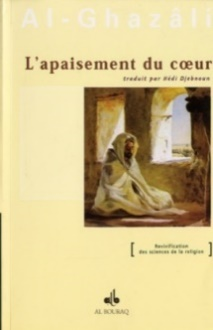
\includegraphics{Images/image002.jpg}
\sidecaption{essai}
\end{figure}


\begin{table}[h!]
\resizebox{\textwidth}{!}{%
\small
\begin{tabular}{p{2cm}p{4cm}p{4cm}}
\toprule
essai & essai & essai \\
\midrule
essai & essai & essai \\
\bottomrule

\end{tabular}%
}
\sidecaption{essai}
\end{table}

\begin{longtable}{p{6cm}p{6cm}}
\toprule
\endhead
«~Quiconque obéit au Messager obéit certainement à Allah~». 
&\TArabe{ مَّن
يُطِعِ الرَّسُولَ فَقَدْ أَطَاعَ اللَّهَ }\\
\bottomrule
\end{longtable}
\part{Fondations de l'Islam - Emmanuel Pisani}
%\begin{comment}

\chapter{Qu'est ce que l'Islam ?}

\section{Calligraphie}


\includegraphics[width=\textwidth]{Images/image011.png}

« Le sens du mot islam est à mettre en relation avec le fait de
rester~''sain et sauf'' et, pour cela, de ne pas avoir d'intention
agressive. Il n'a donc aucun rapport avec le sens de~``soumission''
qu'on prête généralement à ce mot. Le~\emph{muslim}, celui qui fait
montre d'islam, ne fait que se mettre~``sous la sauvegarde'' de Dieu,
car c'est Dieu qui protège et garde en sécurité et en vie. Dans le
Coran, le mot islam est à comparer avec le mot~``imân'', qui a un sens
plus fort car il renvoie au fait d'être fidèle mais aussi d'agir en
conséquence. L'idée de soumission n'émerge que plus tard, lorsque la
société initiale se transforme en empire et que commence à s'imposer le
juridisme du sunnisme, à la fin du IX\textsuperscript{e}~siècle. » Jacqueline Chabbi



« Cette calligraphie est structurée autour d'un cercle, avec un axe au
milieu, comme une colonne vertébrale à l'intérieur d'un être humain. En
haut et en bas, deux courbes, de la même largeur, vont dans des
directions opposées. C'est un mouvement que l'on trouve dans de
nombreuses  oeuvres d'art, chez Michel-Ange comme dans le yin et le
yang\ldots{} Pour moi, il n'y a pas un islam, mais des islams très
différents les uns des autres, selon les époques et les pays. Cette
ouverture est une manière de montrer que l'islam est pluriel. Quant au
bleu, il vient de la mosquée de mon enfance, dans une ville du désert
irakien. Tout y était de couleur ocre, sauf cet édifice recouvert de
céramiques couleur cobalt et turquoise. C'est un bleu qui reste chaud,
comme celui de la mer Méditerranée\ldots{} » Hassan Massoudy


\vide{introduction-1}{%
\section{Introduction}\label{introduction-1}}

Salama~: Islam

Partir de ce que cela veut dire~?

Religion à partir des grands penseurs classiques puis contemporains
(Airn Boubakeur)~: une construction.

Enfin dans une dernière partie, une méthodologie. Comment fait-on pour
entrer dans un autre univers. Penser l'altérité~? Comment fait-on quand
on est musulman quand on veut entrer dans une réalité différente.


\vide{leuxe7on-introductive-aux-fondations-de-lislam}{%
\section{Leçon introductive aux fondations de
l'islam}\label{leuxe7on-introductive-aux-fondations-de-lislam}}
objectifs:
Comment aborder l'islam du point de vue
musulman
Bien voir l'importance de la culture du
désert pour saisir l'islam
L'islam se comprend en référence à la
langue arabe, langue sémitique.
L'islam se décline au
pluriel


\subsection{La Mecque et l'Arabie}

Pascal remarquait que l'islam est né dans 
\begin{quote}
    «~un canton retiré de
l'univers~».
\end{quote} 
Certes, La Mecque est au 6\textsuperscript{e} siècle de
notre ère un village du désert, mais il n'est pas pour autant
déserté\sn{~Ziauddin Sardar, \emph{Histoire de La Mecque. De la
  naissance d'Abraham au XXI\textsuperscript{e} siècle}, Paris, Payot,
  2015.}. Selon l'historiographie musulmane, La Mecque est un lieu de
pèlerinage multiconfessionnel. Il abrite une Ka`ba, un temple sacré, aux
nombreuses statues et icônes. L'historienne Jacqueline Chabbi remarque
dans une étude documentée\sn{ Jacqueline Chabbi, \emph{Le Seigneur
  des tribus. L'islam de Mahomet,} Paris, Noêsis, 1997.} que La Mecque
est répertoriée pour la première fois au IIe siècle par le géographe
Ptolémée dans son ouvrage \emph{Géographie} sous le nom de
Makoraba\sn{Ptolémée, \emph{Géographie}, VI, 7, 31-37.}. Elle y
retrouve la racine \emph{baraka} -- lisez le nom de la ville à l'envers
en ne retenant que les consonnes et en abandonnant le préfixe `ma'
propre aux noms de lieux, ça marche -- ce qui suggère la présence
miraculeuse en ce lieu désertique d'une eau pérenne, signe d'une
bénédiction. Selon Christoph Luxenberg cependant, il faut lire derrière
La Mecque la racine syriaque \emph{makk} désignant une vallée. Ce
rapprochement n'est pas anodin~: s'il atteste, selon l'auteur, du
caractère syro-araméen du lieu {,} il lui permet aussi de
rattacher la naissance de l'islam à la tradition syriaque\sn{~Christoph
  Luxenberg, \emph{The Syro-Aramaic reading of the Koran~: a
  Contribution to the Decoding of the language of the Koran}, éd.
  Schiler, 2007, p. 327.} -- et donc, si l'on veut comprendre l'islam et
le Coran, il va falloir recourir au syriaque, c'est ce qu'il cherche à
montrer dans son livre --.
Plus largement, la perception de La Mecque comme lieu de pèlerinage
pluriconfessionnel permet de rendre compte de l'existence dans le Coran
et la tradition musulmane de thématiques, de récits, de personnages
communs à la tradition judéo-chrétienne. Il apparaît en effet que des
juifs et des chrétiens passaient à La Mecque. S'il est difficile
d'attester de l'existence d'une communauté, des chrétiens semblent y
avoir habité. En tous les cas, la tradition musulmane
l'affirme\sn{~Emmanuel Pisani, «~Waraqa Ibn Nawafal~: un chrétien
  aux origines de l'islam~?~», dans \emph{La Règle herméneutique}, n°36,
  décembre 2014, p. 31-53.} -- cette affirmation n'en fait pas une
vérité historique. Elle peut aussi être véhiculée pour des motifs
apologétiques, nous y reviendrons quand nous aborderons la biographie du
Prophète Muḥammad (qu'on appelle en arabe Sīra) -- . Quel rôle les juifs
et les chrétiens ont-ils pu jouer dans la prédication de l'islam à son
origine~? Quel rôle leur est-il donné dans le Coran~? Autrement dit,
l'islam est-il un abrahamisme, s'inscrivant dans la théologie biblique
ou est-il une religion distincte du judaïsme et du christianisme même
s'il réinvestit certains personnages de la tradition biblique~? On voit
que la connaissance de l'islam, de ses croyances, de ses pratiques, de
sa tradition n'est pas sans conséquence pour la théologie. On ne peut
pas réfléchir en théologie sur le sens de l'islam, sur ce que veut dire
du point de vue chrétien la présence de cette religion et de son
développement, sans aborder ces questions.

Ce cours doit donc servir de base aux théologiens, mais il vise aussi à
donner une connaissance de l'islam de l'intérieur. Il ne s'agit pas pour
autant d'un «~catéchisme musulman~». De la même manière que la foi en
théologie chrétienne est éclairée et épurée par la lumière de la raison,
il s'agira de présenter la foi et les pratiques de l'islam à partir des
penseurs et théologiens musulmans et de leur recours à la raison. En ce
sens, nous montrerons que si les penseurs du wahhabisme -- c'est-à-dire
de l'islam promu en Arabie saoudite -- réduisent le \emph{credo}
musulman à un ensemble de vérités à croire `sans discussion', il s'agit
là d'un affaiblissement considérable de la tradition musulmane et de sa
richesse.

En tenant compte de l'histoire, des sources musulmanes et
extra-musulmanes, des manuscrits du Coran et des différences manuscrites
pouvant exister, des recherches en épigraphie et de leur enseignement
sur l'histoire de la langue arabe, de la confrontation des
herméneutiques et des lectures historiques au sein du monde musulman,
des différences de courants juridiques, dogmatiques, spirituels et
mystiques, nous soulignerons la \emph{diversité}, l'\emph{hétérogénéité}
de l'islam.

L'affirmation selon laquelle l'islam, c'est simple~: il s'agit
d'affirmer que «~Dieu est Un et que Muḥammad est son Prophète~» n'est
peut-être pas si «~simple~». Or, mon «~intime conviction~» est que la
prise de conscience de cette diversité, de cette richesse au sein de
l'islam est aujourd'hui une nécessité incontournable à l'heure où l'on
assiste à son uniformisation, à l'élaboration d'un \emph{credo}
mondialisé, laissant croire qu'il est le seul \emph{credo} autorisé, la
seule définition originelle de ce qu'est l'islam. L'étude des fondations
et des fondements de l'islam ouvre un regard autre, plus que jamais
nécessaire, sachant que les premières victimes d'une vision uniforme de
l'islam sont les musulmans eux-mêmes.


\subsection{Définition musulmane de l'islam
}
\label{duxe9finition-musulmane-de-lislam}

Qu'est-ce que l'islam~? Pour répondre à cette question, il est une
méthodologie particulière suivie par les savants musulmans au cours de
l'histoire que nous nous proposons de suivre. Elle donne d'ores et déjà
un indice sur la manière de procéder pour répondre à une question posée.
Dans un premier temps, on prend soin de partir de la langue arabe, de la
racine du mot et de la constellation sémantique qu'elle désigne. Dans un
deuxième temps, on ouvre le Coran pour voir ce que le Livre sacré dit
lui-même du mot interrogé, puis on ouvre la tradition prophétique,
c'est-à-dire les paroles que Muḥammad a tenues en présence de ses
compagnons depuis le début de la révélation coranique en 610 jusqu'à sa
mort. Enfin, on se réfère à d'éminents penseurs avant de proposer
éventuellement une formulation renouvelée, modernisée. Nous allons donc
suivre leur démarche.

Une première manière de définir l'islam, consiste donc à partir du champ
sémantique de la racine, donc de la langue arabe. Cette langue est
intrinsèquement liée à l'islam. Rašīd Riḍā, penseur égyptien et
réformateur du début du XXème siècle, écrit~:

\begin{quote}
«~Une des grandes réformes religieuses et sociales de l'islam a été de
réaliser l'unité linguistique. Il a fait de l'arabe sa langue, la langue
de toutes les races qui l'avaient adopté. L'islam et la langue arabe se
sont toujours prêté un mutuel appui. Sans l'Islam, la langue arabe se
fût altérée, à l'exemple des autres langues, et comme elle-même l'avait
été auparavant. Sans la langue arabe, l'Islam n'eut pas manqué de voir
les hommes s'éloigner de plus en plus de ses doctrines et de se morceler
lui-même en une infinité de sectes s'excommuniant réciproquement
(\ldots) La langue arabe n'est pas l'apanage des Arabes, fils de Qaḥtān,
mais bien celle de tous les musulmans, des peuples même non arabes --
comme elle est aussi celle des Arabes non musulmans~»\sn{Rašīd
  Riḍā, \emph{Le Califat}, p. 149}.
\end{quote}

\subsubsection{ Le recours à la langue arabe} \mn{Plusieurs dictionnaires sont précieux en la matière. Le
  dictionnaire incontournable pour les arabisants est le \emph{Lisān
  al-`arab} d'Ibn Manẓūr. Il y a 15 volumes édités à Beyrouth. On en
  trouve une version en ligne sur le site
  \href{http://www.baheth.info/}.
  En français, le \emph{Dictionnaire arabe-français} de Kazimirski fait
  référence car il prend en compte l'arabe classique, l'arabe ancien --
  ce que ne fait pas le Larousse qui se limite à l'arabe moderne. Pour
  les textes anciens, le Kazimirski est indispensable.}

En arabe, chaque mot est composé d'une racine, la plupart du temps
structurée par trois consonnes -- nous reviendrons dans la deuxième
leçon sur la spécificité de la langue arabe et de sa dimension
sémitique. Pour l'heure, remarquons que dans le mot
i\textbf{sl}a\textbf{m}, on trouve donc la racine Sa.La.Ma. Quel est son
champ de significations~?

 
\paragraph{Forme I~: al-salāmat (\TArabe{سلامة}) :
absence de défaut, droiture, intégrité, perfection, salut.
}

\emph{Al-salāmat} désigne un état parfait, l'absence de vices ou de
défauts.

\paragraph{ Forme I : \emph{al-salām}} (\textbf{\TArabe{سلام}})~: salut, sécurité,
paix

C'est l'idée de paix absolue, de paix totale, l'assurance de la
sécurité.

Dār al-salām, Demeure de la Paix, est aussi un nom pour désigner le
Paradis. C'est aussi le surnom de Bagdad (\emph{madīnat al-salām}).

On retrouve le mot dans la salutation quotidienne du musulman à un
autre.


\paragraph{ Forme II : taslīm
(\TArabe{تسليم})~}

\emph{Taslīm} est un nom d'action. On y trouve l'idée de conserver
intact, sain et sauf, mais aussi de protéger contre un danger.

Avec la préposition \emph{min}, il signifie sauver quelqu'un, le tirer
d'un danger.

\emph{Taslīm} désigne aussi le salut adressé une personne, le fait de
lui dire «~la paix soit avec toi~». Le \emph{taslīm} est aussi la fin de
la prière musulmane avec l'invocation à droite et à gauche de la
formule~: «~\emph{al-Salāmu ʿalaykum wa-raḥmatu Llāhi wa-barakātuhu~}»~:
idée de demander la paix de Dieu, sa miséricorde, ses
bénédictions.À la fin de la prière, le priant tourne sa tête à
  droite puis à gauche, saluant les anges, et recourant à cette formule.
  Dans certains rites, comme le rite malikite (c'est le rite majoritaire
  dans les pays du Maghreb, on y reviendra), il ne dit que
  \emph{al-Salāmu}. Cette formule est inspirée d'un \emph{ḥadīṯ}
  (prononcer hadiiith), c'est-à-dire une parole de Muḥammad, rapportée
  par Ibn Hajr.

\paragraph{Forme X~: istislām (\TArabe{(استسلام)}:
s'abandonner, se soumettre, se livrer, rendre les armes, obéir sans
opposition.} Le terme renvoie à une obéissance sans condition. Il s'agit de suivre le
chemin droit sans s'en écarter.
Obéissance peut aussi se dire al-ṭā`a~: c'est l'obéissance, la subordination mais ce terme suppose la possibilité, sous certaines conditions, de ne pas obéir.
\sn{ J'obéis à mon patron dans le cadre de mon travail~mais pas en dehors. Le terme recouvre aussi celui d'obéissance sous couvert de résistance intérieure. cf. Bertolt Brecht, Geschichten vom Herrn Keuner~: Massnahmen gegen die Gewalt et la question de l'agent  -- veux-tu me servir -- et lui de ne pas répondre, mais de mettre la couverture le soir, de chasser les mouches, de le servir sept années durant, puis quand il eut crevé de dire~: «~Nein~! ». En islam~: je fais ma prière, par obéissance, mais pas avec le coeur.}



À l'inverse, \emph{al-istislām} est l'obéissance absolue, sans
résistance, sans la moindre contrainte ou le moindre frein
psychologique, spirituel, etc\ldots{} Elle prend deux dimensions~:
\begin{itemize}
    \item l'obéissance à Dieu dans l'acte d'adoration et dans le suivi de sa Loi.
    \item L'obéissance au prophète Muḥammad.
\end{itemize}



\paragraph{ Forme IV~ : islām (\TArabe{إسلام})~:
conserver intact, sain et sauf.
}

L'islam renvoie donc à ce qui sauve, qui est pur, intégral, originel,
préservé d'erreurs ou de scories, ce qui est dans le vrai chemin. Islām
implique l'idée d'obéissance, d'abandon à Dieu. Traduit parfois par
soumission, en référence à sa forme \emph{istislām}, il s'agit d'une
soumission intégrale à Dieu et à Dieu seul. C'est une 
\begin{quote}
    «~remise confiante
de soi à Dieu~»\sn{Mohammed Talbi et Gwendoline Jarczyk,
  \emph{Penseur libre en islam}, Paris, Albin Michel, 2002, p. 158.} ou
encore l'«~adhésion consciente et active à la Paix (\emph{salām}) de
Dieu~». 
\end{quote}Étymologiquement, \emph{islām} renvoie à une attitude religieuse
universelle. Elle est une vertu commune à tous les hommes. Il s'ensuit
que certains \emph{`ulamā'} (\emph{ce sont des savants}) définissent
l'islam non comme une religion mais comme l'attitude spirituelle commune
à toute l'humanité. Dans cette perspective, l'islam se serait mué en
religion, mais il n'aurait pas dû l'être~; il aurait dû rester un rappel
(\emph{ḏikr}) à se souvenir de Dieu, à adhérer à lui avec confiance et
abandon\sn{Soubhi Saleh, \emph{Réponse de l'islam aux défis de
  notre temps}, Beyrouth, Arabelle, 1979, p. 102. Voir aussi Muḥammad
  al-Ġazālī, \emph{Al-ta`assub wa al-tasāmuh bayna al-masīhiyya wa
  al-islām} {[}Fanatisme et tolérance entre le christianisme et
  l'islam{]}, Damas, 2005, p . 77.}.

\vide{le-mot-islux101m-ux625ux633ux644ux627ux645-dans-le-coran}{%
\subsubsection{{Le mot islām \TArabe{ (إسلام)}~: dans le Coran}}\label{le-mot-islux101m-ux625ux633ux644ux627ux645-dans-le-coran}}

Dans le Coran, la racine Sa.La.Ma se retrouve 157 fois. On la trouve
notamment dans le nom \emph{muslim}, celui qui suit l'islam, qui a donné
en français \textbf{«}~musulman~\textbf{»}. En revanche, le mot islam
\TArabe{إِسْلَامِ} lui-même, \emph{masdar} (nom actif) de
4\textsuperscript{ème} forme du verbe \emph{aslama}, le fait de faire
acte d'islam, n'est utilisé que 8 fois.

Nous allons reprendre les versets où le mot apparaît et voir quels sont
les sens qui semblent émerger dans le contexte immédiat de son emploi.
On s'appuiera aussi sur les versets comprenant le verbe \emph{aslama}.
Précisons que cette démarche devrait en toute rigueur être accompagnée
de la lecture des commentaires coraniques traditionnels pour comprendre
comment les musulmans lisent les versets référés et comprennent le mot
\emph{islām}.

\begin{table}[h!]
    \centering
     \footnotesize
   \begin{tabular}{p{0.35\textwidth}p{0.3\textwidth}p{0.28\textwidth}}



S.3, 19~: «~Certes, la religion auprès d'Allah, c'est l'islam. Ceux
auxquels le Livre a été apporté ne se sont disputés, par agressivité
entre eux, qu'après avoir reçu la science. Et quiconque ne croit pas aux
signes d'Allah... alors Allah est prompt à demander compte!~» &
\TArabe{إِنَّ الدِّينَ عِنْدَ اللَّهِ \textbf{الْإِسْلَامُ} وَمَا اخْتَلَفَ
الَّذِينَ أُوتُوا الْكِتَابَ إِلَّا مِنْ بَعْدِ مَا جَاءَهُمُ الْعِلْمُ
بَغْيًا بَيْنَهُمْ وَمَنْ يَكْفُرْ بِآَيَاتِ اللَّهِ فَإِنَّ اللَّهَ
سَرِيعُ الْحِسَابِ} & Inna a\textbf{l}ddeena AAinda All\underline{a}hi
\textbf{alisl\underline{a}mu} wam\underline{a}~ikhtalafa
alla\underline{th}eena ootoo alkit\underline{a}ba ill\underline{a}~min
baAAdi m\underline{a}~j\underline{a}ahumu alAAilmu baghyan baynahum
waman yakfur bi\underline{a}y\underline{a}ti All\underline{a}hi fainna
All\underline{a}ha sareeAAu
al\underline{h}is\underline{a}b\textbf{i}~(⁎) \\


S.3, 20~: S'ils te contredisent, dis leur : "Je me suis entièrement
soumis à Allah, moi et ceux qui m'ont suivi". Et dis à ceux à qui le
Livre a été donné, ainsi qu'aux illettrés : "Avez-vous embrassé l'Islam?
" S'ils embrassent l'Islam, ils seront bien guidés. Mais, s'ils tournent
le dos... Ton devoir n'est que la transmission (du message). Allah, sur
{[}Ses{]} serviteurs est Clairvoyant~». & \TArabe{فَإِنْ حَاجُّوكَ فَقُلْ
أَسْلَمْتُ وَجْهِيَ لِلَّهِ وَمَنِ اتَّبَعَنِ وَقُلْ لِلَّذِينَ أُوتُوا
الْكِتَابَ \textbf{وَالْأُمِّيِّينَ} أَأَسْلَمْتُمْ فَإِنْ أَسْلَمُوا
فَقَدِ اهْتَدَوْا وَإِنْ تَوَلَّوْا فَإِنَّمَا عَلَيْكَ الْبَلَاغُ
وَاللَّهُ بَصِيرٌ بِالْعِبَادِ} & Fain~\underline{ha}jjooka faqul
aslamtu wajhiya lill\underline{a}hi wamani ittabaAAani waqul
lilla\underline{th}eena ootoo alkit\underline{a}ba
wa\textbf{a}lommiyyeena \textbf{aaslamtum} fain \textbf{aslamoo} faqadi
ihtadaw wain tawallaw fainnam\underline{a}~AAalayka
albal\underline{a}ghu wa\textbf{A}ll\underline{a}hu ba\underline{s}eerun
bi\textbf{a}lAAib\underline{a}d\textbf{i} \\
\end{tabular}
\caption{versets comprenant le verbe \emph{aslama}. S 3,19-20}
\end{table}


\begin{table}[h!]
    \centering
    \footnotesize
  \begin{tabular}{p{0.35\textwidth}p{0.3\textwidth}p{0.28\textwidth}}

S. 3, 85~: Et quiconque désire une religion autre que l'Islam, se verra
refuser son choix, et il sera, dans l'au-delà, parmi les perdants~». &
\TArabe{وَمَن يَبْتَغِ غَيْرَ الْإِسْلَامِ دِينًا فَلَن يُقْبَلَ مِنْهُ
وَهُوَ فِي الْآخِرَةِ مِنَ الْخَاسِرِينَ} & Waman yabtaghi ghayra
alisl\underline{a}mi deenan falan yuqbala minhu wahuwa fee
al\underline{a}khirati mina alkh\underline{a}sireen\textbf{a}~( \\
S.5, 3~: «~Et aujourd'hui, j'ai parachevé pour vous votre religion et
j'agrée l'islam comme religion~». & \TArabe{الْيَوْمَ أَكْمَلْتُ لَكُمْ
دِينَكُمْ وَأَتْمَمْتُ عَلَيْكُمْ نِعْمَتِي وَرَضِيتُ لَكُمُ
الْإِسْلَامَ} & AAalaykum niAAmatee wara\underline{d}eetu lakumu
alisl\underline{a}ma deenan (religion) famani i\underline{dt}urra fee
makhma\underline{s}atin ghayra mutaj\underline{a}nifin liithmin fainna
All\underline{a}ha ghafoorun ra\underline{h}eem\textbf{un}~(⁎) \\
6, 125~: «~Et puis, quiconque Allah veut guider, Il lui ouvre la
poitrine à l'Islam. Et quiconque Il veut égarer, Il rend sa poitrine
étroite et gênée, comme s'il s'efforçait de monter au ciel. Ainsi Allah
inflige Sa punition à ceux qui ne croient pas~». & \TArabe{فَمَنْ يُرِدِ
اللَّهُ أَنْ يَهدِيَهُ يَشْرَحْ صَدْرَهُ لِلْإِسْلَامِ وَمَنْ يُرِدْ
أَنْ يُضِلَّهُ يَجْعَلْ صَدْرَهُ ضَيِّقًا حَرَجًا كَأَنَّمَا يَصَّعَّدُ
فِي السَّمَاءِ كَذَلِكَ يَجْعَلُ اللَّهُ الرِّجْسَ عَلَى الَّذِينَ لَا
يُمِنُونَ} & Faman yuridi All\underline{a}hu an yahdiyahu
yashra\underline{h}~\underline{s}adrahu lilisl\underline{a}mi waman
yurid an yu\underline{d}illahu
yajAAal~\underline{s}adrahu~\underline{d}ayyiqan~\underline{h}arajan
kaannam\underline{a}~ya\underline{ss}aAAAAadu fee
a\textbf{l}ssam\underline{a}i ka\underline{tha}lika yajAAalu
All\underline{a}hu a\textbf{l}rrijsa
AAal\underline{a}~alla\underline{th}eena
l\underline{a}~yuminoon\textbf{a}~(⁎) \\
\end{tabular}

\end{table}
\begin{table}[h!]
    \centering
     \footnotesize
 \begin{tabular}{p{0.35\textwidth}p{0.3\textwidth}p{0.28\textwidth}}

9, 74~: «~Ils jurent par Allah qu'ils n'ont pas dit ce qu'ils ont
proféré, alors qu'en vérité ils ont dit la parole de la mécréance et ils
ont été infidèles après leur conversion à l'islam. Ils ont projeté ce
qu'ils n'ont pu accomplir. Mais ils n'ont pas de reproche à faire si ce
n'est qu'Allah - ainsi que Son messager - les a enrichis par Sa grâce.
S'ils se repentaient, ce serait mieux pour eux. Et s'ils tournent le
dos, Allah les châtiera d'un douloureux châtiment, ici-bas et dans
l'au-delà; et ils n'auront sur terre ni allié ni secoureur~». &
\TArabe{يَحْلِفُونَ بِاللَّهِ مَا قَالُوا وَلَقَدْ قَالُوا كَلِمَةَ
الْكُفْرِ وَكَفَرُوا بَعْدَ إِسْلَامِهِمْ وَهَمُّوا بِمَا لَمْ يَنَالُوا
وَمَا نَقَمُوا إِلَّا أَنْ أَغْنَاهُمُ اللَّهُ وَرَسُولُهُ مِنْ فَضْلِهِ
فَإِنْ يَتُوبُوا يَكُ خَيْرًا لَهُمْ وَإِنْ يَتَوَلَّوْا يُعَذِّبْهُمُ
اللَّهُ عَذَابًا أَلِيمًا فِي الدُّنْيَا وَالْآَخِرَةِ وَمَا لَهُمْ فِي
الْأَرْضِ مِنْ وَلِيٍّ وَلَا نَصِيرٍ} & Ya\underline{h}lifoona
bi\textbf{A}ll\underline{a}hi m\underline{a}~q\underline{a}loo walaqad
q\underline{a}loo kalimata alkufri wakafaroo baAAda
isl\underline{a}mihim wahammoo bim\underline{a}~lam yan\underline{a}loo
wam\underline{a}~naqamoo ill\underline{a}~an aghn\underline{a}humu
All\underline{a}hu warasooluhu min fa\underline{d}lihi fain yatooboo
yaku khayran lahum wain yatawallaw yuAAa\underline{thth}ibhumu
All\underline{a}hu AAa\underline{tha}ban aleeman fee
a\textbf{l}dduny\underline{a}~wa\textbf{a}l\underline{a}khirati
wam\underline{a}~lahum fee alar\underline{d}i min waliyyin
wal\underline{a}~na\underline{s}eer\textbf{in}~(⁎) \\
S. 39, 22~: «~Est-ce que celui dont Allah ouvre la poitrine à l'Islam et
qui détient ainsi une lumière venant de Son Seigneur... Malheur donc à
ceux dont les coeurs sont endurcis contre le rappel d'Allah. Ceux-là sont
dans un égarement évident.~» & \TArabe{أَفَمَنْ شَرَحَ اللَّهُ صَدْرَهُ
لِلْإِسْلَامِ فَهُوَ عَلَى نُورٍ مِنْ رَبِّهِ فَوَيْلٌ لِلْقَاسِيَةِ
قُلُوبُهُمْ مِنْ ذِكْرِ اللَّهِ أُولَئِكَ فِي ضَلَالٍ مُبِينٍ} & Afaman
shara\underline{h}a All\underline{a}hu~\underline{s}adrahu
lilisl\underline{a}mi fahuwa AAal\underline{a}~noorin min rabbihi
fawaylun lilq\underline{a}siyati quloobuhum min~\underline{th}ikri
All\underline{a}hi ol\underline{a}ika
fee~\underline{d}al\underline{a}lin mubeen\textbf{in}~(⁎) \\
\end{tabular}

\end{table}
\begin{table}[h!]
    \centering
    \footnotesize
 \begin{tabular}{p{0.35\textwidth}p{0.3\textwidth}p{0.28\textwidth}}

S. 49, 14~:~«~Les Bédouins ont dit: \textbf{`\,`Nous avons la foi'\,'}.
Dis: `\,`Vous n'avez pas encore la foi. Dites plutôt: Nous nous
\textbf{sommes simplement soumis,} car la foi n'a pas encore pénétré
dans vos coeurs. Et si vous obéissez à Allah et à Son messager, Il ne
vous fera rien perdre de vos  oeuvres'\,'. Allah est Pardonneur et
Miséricordieux~». & \TArabe{قَالَتِ الْأَعْرَابُ آَمَنَّا قُلْ لَمْ
تُؤْمِنُوا وَلَكِنْ قُولُوا أَسْلَمْنَا وَلَمَّا يَدْخُلِ الْإِيمَانُ
فِي قُلُوبِكُمْ وَإِنْ تُطِيعُوا اللَّهَ وَرَسُولَهُ لَا يَلِتْكُمْ مِنْ
أَعْمَالِكُمْ شَيْئًا إِنَّ اللَّهَ غَفُورٌ رَحِيمٌ} &
Q\underline{a}lati
alaAAr\underline{a}bu~\textbf{\underline{a}mann\underline{a}}~qul lam
tuminoo wal\underline{a}kin qooloo
\textbf{aslamn\underline{a}}~walamm\underline{a}~yadkhuli
aleem\underline{a}nu fee quloobikum wain tu\underline{t}eeAAoo
All\underline{a}ha warasoolahu l\underline{a}~yalitkum min
aAAm\underline{a}likum shayan inna All\underline{a}ha ghafoorun
ra\underline{h}eem\textbf{un} \\
S. 49, 17~: «~Ils te rappellent leur conversion à l'Islam comme si
c'était une faveur de leur part. Dis: `Ne me rappelez pas votre
conversion à l'Islam comme une faveur. C'est tout au contraire une
faveur dont Allah vous a comblés en vous dirigeant vers la foi, si
toutefois vous êtes véridiques'. & \TArabe{يَمُنُّونَ عَلَيْكَ أَنْ
أَسْلَمُوا قُلْ لَا تَمُنُّوا عَلَيَّ إِسْلَامَكُمْ بَلِ اللَّهُ يَمُنُّ
عَلَيْكُمْ أَنْ هَدَاكُمْ لِلْإِيمَانِ إِنْ كُنْتُمْ صَادِقِينَ} &
Yamunnoona AAalayka an aslamoo qul l\underline{a}~tamunnoo AAalayya
isl\underline{a}makum bali All\underline{a}hu yamunnu AAalaykum an
had\underline{a}kum lileem\underline{a}ni in
kuntum~\underline{sa}diqeen\textbf{a} \\
S. 61, 7~: «~Et qui est plus injuste que celui qui invente un mensonge
contre Allah, alors qu'il est appelé à l'Islam? Et Allah ne guide pas
les gens injustes~». & \TArabe{وَمَنْ أَظْلَمُ مِمَّنِ افْتَرَى عَلَى
اللَّهِ الْكَذِبَ وَهُوَ يُدْعَى إِلَى الْإِسْلَامِ وَاللَّهُ لَا
يَهْدِي الْقَوْمَ الظَّالِمِينَ} & Waman a\emph{\underline{th}}lamu
mimmani iftar\underline{a}~AAal\underline{a}~All\underline{a}hi
alka\underline{th}iba wahuwa
yudAA\underline{a}~il\underline{a}~\textbf{alisl\underline{a}mi}
wa\textbf{A}ll\underline{a}hu l\underline{a}~yahdee alqawma
a\textbf{l}\underline{\emph{thth}a}limeen\textbf{a} \\

\end{tabular}

\end{table}

Un premier constat s'impose, ces références au mot \emph{islām} dans le
Coran ou au verbe \emph{aslama} permettent d'ores et déjà d'en préciser
le sens, ne serait-ce que par jeu d'opposition, d'antinomie ou de
rapprochement lexical.


\begin{itemize}
\item
  Ainsi, une série voit en l'islam un \textbf{appel divin}. Il est
  précisé être une guidance~: S.61, 7.
\item
  D'autres versets associent \emph{islām} à religion~(\emph{dīn}) : 5,
  3~; 3, 19~; 3, 85. L'islam est donné par Dieu dans un processus
  temporel aux arabes. Il est agréé comme religion par Dieu. Notons qu'à
  la lumière de ce verset il n'est pas dit que l'islam se substitue aux
  autres religions. Le parachèvement est celui de l'islam lui-même. Le
  verset 3, 19 semble être exclusiviste~:~«~La religion auprès de Dieu,
  c'est l'islam~», mais tout dépend s'il faut bien comprendre \emph{dīn}
  par religion. Mahmad al-Alūsī (m. 1853) commente les avis en disant
  que le mot islam désigne le principe d'abandon propre aux croyants.
\item
  Un troisième sens émerge dans un jeu d'opposition notamment ici au
  \emph{kufr}, c'est-à-dire à la mécréance, l'infidélité à l'unicité
  divine, et l'appel à la conversion~: S. 9, 74~; 49, 17.
\item
  Enfin, une opposition est établie entre la foi (\emph{imān}) et
  l'\emph{islām}. Il n'y a pas synonymie. Selon le verset indiqué S. 49,
  14~, on peut être musulman sans être croyant. Le contraire est-il
  vrai~? Question très importante pour la théologie musulmane et dans
  ses conséquences pour aujourd'hui par rapport à la question du statut
  de l'autre. Nous y reviendrons.
\end{itemize}

On voit à la lumière de ces versets l'établissement de distinctions,
l'articulation de différents couples sémantiques en rapport avec
l'islam. Ainsi par exemple, l'\emph{islām} est une religion (\emph{dīn})
parmi d'autres~; l'islam est considéré comme un chemin donné par Dieu,
une faveur qui n'est pas donnée à tous. Autre opposition, entre
l'\emph{islām} et le \emph{kufr}. Le Coran souligne l'existence d'hommes
redevenus infidèles après s'être converti à l'islam, il indique aussi la
possibilité du repentir. On retrouve aussi l'idée de vérité et de
justice associée à l'islam.

\vide{din-religion-plus-large-voie-coutume-jugement}{%
\paragraph{Din~: religion~? plus large~: voie, coutume,
jugement}\label{din-religion-plus-large-voie-coutume-jugement}}

Cette étude des mots \emph{islām} et \emph{dīn} a fait l'objet d'une
recherche pour une thèse qui a été soutenue à la fin du mois de
septembre 2016~par Cyrille Moreno, sous la direction d'Éric Geoffroy et
avec dans le jury Moezzi, Denis Gril, Makram Abbès, Jean-Louis Schlegel.
Elle est intitulée~: \emph{Analyse Littérale des termes dîn et islâm
dans le Coran -- Dépassement spirituel du religieux et nouvelles
perspectives exégétiques.}

Elle remet en cause bien des données de l'islamologie classique, à
commencer par la signification étymologique du mot \emph{dīn}. L'auteur
montre qu'il a plusieurs origines~: il dérive selon les versets soit de
\emph{dên} en pehlevi, du concept avestique de daênâ, soit de
l'araméo-hébraïque \emph{dân\textbf{,}} soit de la racine arabe
\emph{dāna}.

Il trouve 15 significations~parmi lesquelles foi, voie, rétribution,
croyance, culte, rituel, tradition, coutume, obéissance, sentence,
jugement, usage. Il est donc réducteur de ne retenir du mot \emph{dīn}
dans le Coran que celui de religion, culte, voire rétribution. Il
remarque que \emph{dīn} n'est pas employé pour désigner une religion ou
une nouvelle religion. Il en conclut que le Coran ne définit pas une
nouvelle religion, mais une nouvelle foi. L'idée que \emph{dīn} renvoie
à une religion est postérieure au Coran. Quant au mot \emph{islām}, il
signifie «~voie spirituelle~». Il relève de l'ordre intérieur,
ésotérique. Il est avant tout spirituel.

\vide{le-recours-uxe0-une-parole-prophuxe9tique}{%
\subsubsection{1.3 Le recours à une parole
prophétique}\label{le-recours-uxe0-une-parole-prophuxe9tique}}

Dans un fameux \emph{\textbf{ḥadīṯ}} ~:

\begin{Def}[ḥadīṯ]

un \emph{ḥadīṯ} (hadith) est une parole
de Muḥammad, l'ensemble des hadiths forme la \emph{Sunna}

\end{Def}

Muslim rapporte un échange entre Muḥammad et Ğibrīl -- l'ange Gabriel.
L'ange interroge le Prophète sur l'\emph{islām}, l'\emph{īmān} et
l'\emph{iḥsān.} Qu'est-ce qu'être musulman~? Qu'est-ce que la foi
musulmane~? Comment devient-on meilleur musulman~? Muḥammad répond et
donne trois définitions fondamentales \sn{Muslim, \emph{Ṣaḥīḥ}, ``Īmān'',
  I, n°5. Voir aussi al-Nawawi, hadith n°2.}. :
\begin{Def}[islām]
«~L'islam (islām), dit-il, consiste à adorer Dieu sans rien Lui
associer, à s'acquitter de la prière prescrite, à verser l'impôt
religieux (zakāt), à jeûner durant le Ramadan~».
\end{Def}

\begin{Def}[īmān]
«~La foi (īmān) consiste à croire en Dieu, à ses Anges, à son Livre, à
sa rencontre dans l'au-delà, à ses prophètes, à la Résurrection~».
\end{Def}

\begin{Def}[iḥsān]

«~La perfection (iḥsān) {[}devenir un parfait musulman{]} consiste à
servir et à adorer Dieu comme s'il était devant vos yeux, car si vous ne
Le voyez pas, Lui vous voit~»
\end{Def}

Dans ce \emph{ḥadīṯ}, l'islam relève de la pratique tandis que la foi
renvoie à l'adhésion à un ensemble de croyances, à un credo
(\emph{`aqīda}). À la lumière de ce \emph{ḥadīṯ}, certains penseurs
musulmans ont soutenu que c'est l'islam qui est premier et non la foi
(\emph{imān})~; l'ordre du questionnement n'est pas anodin~; mais
certains font remarquer qu'il existe un ordre d'intensification de
l'adhésion. Ainsi, on peut pratiquer sans croire. La foi est de l'ordre
de l'intérieur, du coeur, tandis que la pratique relève de l'extérieur~:
celle-ci peut être superficielle et ne pas refléter dans le coeur du
pratiquant ce qu'elle est censée exprimer.

% CULTURE D'ISLAM
 \mn{\url{https://www.franceculture.fr/emissions/cultures-dislam/le-salafisme-en-devenir-0}

    Le wahhabisme : a appauvri l'Islam et la diversité de l'Islam et
    pervertit le salafisme, les pieux ancêtres, les trois premières
    générations de l'Islam.

   8eme siècle critique : question entre l'opinion et l'esprit vs la lettre en
    cas de nouvelles questions

  Ibn tammayyia~: La réfutation des logiciens et Contre Aristote~; pensée profonde même si elle est intransigeante


  Olivier Roy : déculturation car toute culture locale est écrasée ;
    ne reste qu'une Techno-islam, mondialisée, car neutre : des
    tours, des Nikes \ldots{}

   Destruction des mosquées de Mossoul du XIème siècle par DAECH. Ou Abd El Aziz
    qui fonde l'arabie Saoudite et détruit les mausolées des compagnons. Cela est lié à la \textsc{médiation avec Dieu}  : il faut
    empêcher les moyens d'une impiété. 
}
\FloatBarrier
 \paragraph{Ibn Taymiyya},
penseur éminent du treizième siècle soutient que l'on \textsc{peut être musulman
sans être croyant}. Tout le problème sera alors de savoir si l'on peut
être croyant -- avec la profondeur que la foi implique -- sans être
musulman.

Retenez le nom de ce penseur qui reviendra à maintes reprises. Sachez
d'ores et déjà qu'il est une référence incontournable dans les
prédications et enseignements wahhabites. Auteur controversé à
l'enseignement souvent extrémiste (cf. ses \emph{fatwas}), sachez
cependant que la profondeur et la subtilité de son propos ne semblent
pas souvent compris\ldots{} Les grands cheikhs de Médine en caricaturent
la pensée, à commencer par Ibn `Abd al-Wahhab, le fondateur, au
18\textsuperscript{ème} siècle du wahhabisme. Il y a beaucoup de
contresens. Les relever est important, car ils permettent de s'appuyer
sur une autorité reconnue dans le wahhabisme pour dépasser son
enseignement fermé.
 Écoutez ce que dit Abdel Wahhab Meddeb en septembre
  2014 à propos d'Ibn Taymiyya dans l'émission \emph{Culture d'islam}
  consacrée au salafisme sur France culture.


Forts de ces définitions, comment les théologiens musulmans ont-ils
défini l'islam~? Comment aujourd'hui est-il défini ?

\vide{quelques-duxe9finitions-de-penseurs-musulmans}{%
\subsection{{Quelques définitions de penseurs musulmans
}}\label{quelques-duxe9finitions-de-penseurs-musulmans}}

\vide{al-ux11furux11fux101nux12b-740-8161339-1413-encyclopuxe9diste-persan}{%
\subsubsection{{Al-Ğurğānī (740-816/1339-1413),
encyclopédiste persan
}}\label{al-ux11furux11fux101nux12b-740-8161339-1413-encyclopuxe9diste-persan}}

Al-Ğurğānī est connu pour être un encyclopédiste. Il a notamment écrit
un livre fameux, le \emph{Kitāb al-Taʿrīfāt} (\TArabe{تعريفات}),
c'est-à-dire \emph{Le Livre des définitions}\sn{~Ouvrage édité par
  G. Flügel, Leipzig, 1845, publié à Constantinople (1837), Cairo (1866,
  etc.), et St Petersburg (1897). Maurice Gloton en a assuré une
  traduction en français~: Al-Jurjânî, \emph{Le Livre des Définitions},
  traduction, introduction et annotations par Maurice Gloton, Préfacé
  par Pierre Lory, Paris, Albouraq, 2005.}. Reprenons la définition
qu'il donne justement de l'islam~\sn{Al-Jurjânî, \emph{Le Livre des Définitions},
  \emph{op. cit}., p. 68.}.:


\begin{Def}[Islam pour Al-Ğurğānī]
«~L'islām est la soumission, la résignation, la préservation intégrale,
la profession d'islam.

C'est la soumission (\emph{ḫudū`}) à ce que le Messager de Dieu a
notifié et la docilité (\emph{inqiyād}) envers lui. C'est, a-t-on dit
dans le Commentaire coranique appelé al-Kaššāf (de Zaramaḫšarī), la
reconnaissance par la langue (\emph{iqrār}) {[}des 5 piliers du culte{]}
sans adhésion (\emph{muwāṭa'a}) du coeur. Quand le coeur est en accord
avec la langue, il s'agit de l'acte de foi (\emph{īmān}). Tel est l'avis
de l'Imām al-Šāfi`ī. Abû Ḥanīfa n'a fait aucune différence entre ces
deux notions~»
\end{Def}


\begin{itemize}
\item
  On retrouve dans sa définition les connotations sémantiques de la
  racine SaLaMa. La préservation intégrale renvoie à l'absence d'erreur,
  la profession renvoie à l'attitude religieuse, à l'adhésion, au
  témoignage.
\item
  Au coeur de l'islam se trouve mentionné le Messager de Dieu. Il n'est
  pas question des messagers, mais du Messager, même si l'islam
  reconnaît les prophètes de la Bible. Il est question d'un attachement,
  d'une docilité à son enseignement. Dans cette perspective, l'islam, ce
  n'est pas seulement suivre le Coran, le Livre donné par Dieu, mais
  aussi suivre les enseignements du Prophète (Messager = Prophète?). On
  voit ici canonisée la Sunna dont nous avons déjà parlé.
\item
  La distinction entre \emph{islām} et \emph{imān}, entre islam et foi,
  est de nouveau mentionnée. L'islam reste du domaine de l'extériorité,
  de l'expression verbale tandis que seule la foi est du côté de
  l'adhésion du coeur, l'adhésion sincère à ce qui est professé.
\item
  Question cependant disputée et al-\textbf{Ğur}ğ\textbf{ānī} ne prend
  pas position en rapportant deux positions opposées, celle de l'Imām
  \textbf{al-Šāfi`ī} et celle d'\textbf{Abū Ḥanīfa}, tous deux
  fondateurs d'une «~école de jurisprudence~» faisant encore aujourd'hui
  autorité. Nous traiterons des «~écoles de jurisprudence~»
  (\emph{fiqh}) dans un chapitre à venir. Retenez déjà deux d'entre
  elles le shafi'isme et le ḥanifisme.
\end{itemize}

Nous allons à présent exposer la définition donnée par deux penseurs
musulmans contemporains. Le premier a joué un rôle notoire dans
l'émergence de l'islam politique, le second a été un des représentants
de la Grande Mosquée de Paris de 1957 à 1982.

\vide{mawdux16bdux12b-le-grand-penseur-de-lislam-du-xxuxe8me-siuxe8cle}{%
\subsubsection{Mawdūdī, le grand penseur de
l'islam du xx\textsuperscript{ème} siècle
}\label{mawdux16bdux12b-le-grand-penseur-de-lislam-du-xxuxe8me-siuxe8cle}}

Dans son livre \emph{Risāla-é-dīniyāt}, le théologien musulman
pakistanais du vingtième siècle, Mawdūdī (1903-1979), considéré par
beaucoup comme le fondateur de l'islamisme contemporain\sn{Avant
  le 20\textsuperscript{ème} siècle, en français, on utilisait le mot
  islamisme pour définir la religion des musulmans. Mais c'est Louis
  Massignon qui a invité à appeler cette religion par le nom utilisé par
  les musulmans eux-mêmes. Depuis les années 80, on appelle islamisme
  l'islam politique.} -- il est le fondateur du \emph{Jamā'at
al-islamī}, parti islamique voulant constituer un État islamique --,
note que l'islam est la seule de toutes les religions qui ne porte pas
le nom de son fondateur\sn{La traduction française de ce livre
  dont l'original est écrit en ourdu~: Abul A'la Maudoudi,
  \emph{Comprendre l'islam,} Islamic Foundation England, Paris, 1973, p.
  15.} (contrairement au christianisme, au bouddhisme, au zoroastrisme,
ou au judaïsme -- de la tribu de Juda). Particularité qui d'emblée est
située dans un signifiant universel~: «~Le mot islam n'est le propre
d'aucune personne, d'aucun peuple ou pays particuliers. Il n'est pas le
produit d'un esprit humain, il ne se limite pas à une communauté
particulière. C'est une religion universelle qui a pour but de susciter
et de cultiver la qualité et l'attitude de l'islam~»\sn{\emph{Ibid}.,
  p. 15.}.

Pour Mawdūdī, entendre l'islam comme une religion au sens traditionnel
du terme est donc une méprise. L'islam revêt une dimension universelle,
totalisante, qui s'inscrit dans un cadre qui dépasse la réalité humaine
et qui n'est comparable à aucune religion jusqu'alors existante. L'islam
est méta-religion, parachèvement de toutes les religions.

Concrètement, cette qualité et attitude de l'islam consiste en la
soumission et l'obéissance absolue à Dieu et à sa Loi.

Mawdūdī remarque que l'univers est soumis à un ordre, des galaxies à
l'électron, tous suivent l'ordre de la matière. De même, l'homme suit
les lois biologiques. Il grandit, il vieillit. Cet ordre qui régit
l'univers est la loi de Dieu. Comme la création obéit à cette loi
cosmique, tout l'univers suit l'islam. Tout est soumis à cet ordre qu'il
s'agisse du soleil ou des animaux. «~Tout dans l'univers est musulman
car tout obéit aux lois qui lui ont été assignées par Dieu~»\sn{\emph{Ibid}.
  p. 17.} si \emph{(maj.)} bien que pour Mawdūdī, la langue de l'athée,
de celui qui professe que Dieu n'existe pas, est musulmane.

Cependant, la réalité humaine n'est pas exclusivement biologique. Doué
de raison, l'homme est doté du libre arbitre~: «~à l'inverse des autres
créatures, il a reçu la liberté de pensée, d'opinion et
d'action~»\sn{\emph{Ibid}., p. 17}. Si l'homme est biologiquement
musulman, il peut choisir de ne pas l'être spirituellement. C'est ce qui
distingue le croyant du non-croyant. «~Celui qui choisit de reconnaître
son créateur, l'accepte pour Maître unique, se soumet scrupuleusement à
Ses commandements, suit la Loi qu'il a révélée à l'homme pour sa vie
individuelle et sociale devient ainsi un parfait musulman~»\sn{\emph{Ibid}.,
  p. 17}. Il est un parfait musulman dans le sens où il y a harmonie
entre ce qu'il est en son être et ce qu'il confesse, adhère et croit.

Pour Mawdūdī, pour être un parfait musulman, il faut d'abord être
croyant. La foi est première. C'est la connaissance de Dieu qui fait que
l'homme se soumet à Lui, Lui obéit, et cherche à acquérir les attributs
qui Lui sont propres~:

«~Sans la foi, personne ne peut être un vrai musulman. C'est un point
essentiel~; ou plutôt c'est le point de départ. Le rapport entre
l'\emph{islām} et l'\emph{imān} est celui d'un arbre avec sa graine. De
même qu'un arbre ne peut croître sans une graine, de même il n'est pas
possible à l'homme qui n'a pas la foi au départ de devenir un musulman.
Cependant, de même qu'on trouve parfois un arbre qui malgré la graine
semée ne pousse pas, et cela pour des quantités de raisons, ou même s'il
pousse, sa croissance est compromise ou retardée, de même on peut
trouver un homme qui a la foi, mais à cause de certaines faiblesses,
peut ne pas devenir un musulman ferme et véritable~»\sn{\textsc{Mawdudi},
  \emph{Connaître l'islam}, \emph{op. cit}., p. 33.}.

Cette distinction entre l'islam, la foi et la perfection de l'islam
reprend la parole prophétique que nous avons rencontrée. Elle témoigne
d'une articulation entre les notions caractéristiques des
traditionnistes (penseurs attachés aux traditions et aux premiers
commentaires coraniques), mais nous avons vu que cette position est
discutée en théologie musulmane.


\paragraph{Le Cheikh Si Hamza Boubakeur}
(1912-1995), Recteur de la Grande Mosquée de Paris de 1957 à 1982. On trouve une notice biographique sur le site de la Grande Mosquée de
Paris.

Il a publié en 1985 un \emph{Traité moderne de théologie islamique}. Dès
les premières pages de ce \emph{Traité}, Si Hamza Boubakeur s'attache à
donner une définition de l'islam. D'emblée, il définit l'islam dans le
cadre propre du langage de la modernité et de la culture française. D'où
un vocabulaire original qui tranche avec les définitions du Coran, de la
Sunna ou des théologiens classiques.

\begin{quote}
    
«~L'islām, révélation divine\textbf{,} est une religion monothéiste de
vérité spirituelle, de lumière intérieure, d'amour, de fraternité
humaine, de justice sociale\textbf{,} ouverte à toutes les races et à
tous les peuples sans aucune distinction, aux hommes et aux femmes de
toutes les contrées et de tous les siècles, quels que soient le degré de
leur savoir et l'importance de leur fortune. Il implique la foi en un
Dieu Unique et Absolu (\emph{Allahu}) et en la mission de Son Envoyé,
notre Seigneur (SAWS) qu'il a choisi pour la transmission de son message
(Coran). Ce message universel et permanent de liberté, d'égalité, de
fraternité, de charité, de paix, de monothéisme sous la forme la plus
pure, exige \emph{a priori} de l'homme sa soumission inconditionnelle à
Dieu et son abandon total à sa volonté. Tel est d'ailleurs le sens
étymologique du mot Islam. Il se résume en peu de mots : il n'y a qu'un
Dieu ! Muḥammad est un Envoyé de Dieu.

Le Coran exclut toute doctrine religieuse ou philosophique basée sur le
polythéisme, la trinité, l'incarnation, la métempsycose, toute
conception d'un Dieu enfanté ou ayant enfanté, dont l'homme serait
l'image (~!?), toute théorie psychométaphysique d'un panthéisme
universel, toute errance philosophique qui ne reconnaît pas à la foi sa
primauté et à la raison la relativité de sa capacité et les limites de
ses dimensions.

En proclamant l'unicité et la transcendance divines, le Coran condamne
toute association à Dieu d'une autre divinité, d'un quelconque
parèdre\sn{Du grec \emph{paredros} (avoir à côté de). Désigne dans
  l'Antiquité une divinité de rang inférieur.}, tout attachement à un
être, à un objet ou à une cause pouvant faire oublier Dieu ou éloigner
de Lui. Une telle condamnation frappe non seulement l'idolâtrie, mais
encore le culte des fausses divinités modernes qui dépouillent l'homme
de la haute signification qui s'attache à sa vie sur terre~: machinisme,
argent, esprit de jouissance, abus de droit sous toutes ses formes,
racisme, scientisme, lesquels risquent d'entraîner peu à peu l'espèce
humaine vers le chaos moral, l'obscurantisme intellectuel, le vice, la
violence et de la faire régresser vers les abîmes de la primitivité. Les
chimères, l'anagogie\sn{Le ravissement de l'âme dans la
  contemplation des choses divines.} et les mystifications sont
contraires à l'enseignement de l'islam qui donne comme fondements à la
vérité, la raison (\emph{`aql}) et la révélation (\emph{waḥy}).

Il peut, à l'analyse de son ensemble, se définir comme un dogme
(\emph{dīn}), une loi (\emph{sharī`a}), une communauté (\emph{umma}) et
une civilisation (\emph{madaniyya})~»\sn{~Si Hamza
  \textsc{Boubakeur}, \emph{Traité moderne de théologie islamique} :
  contenu doctrinal, ramifications, écoles orthodoxes et hétérodoxes,
  soufisme, théologie comparée, concordances et divergences des
  Écritures révélées, avenir de l'islâm dans le monde , Paris,
  Maisonneuve et Larrose, 3\textsuperscript{ème} édition, 2003, p.
  21-22.}.
\end{quote}

\begin{itemize}
\item
  Dans sa définition, l'islam~revêt une dimension universelle.
\item
  Sa définition s'ancre dans le Coran ou le \emph{ḥadīṯ}, mais elle est
  aussi foncièrement ancrée dans un langage contemporain~: plus encore,
  l'auteur fait coller sa définition de l'islam à la modernité et à son
  paradigme sociologique et politique. Il s'agit aussi de montrer la
  compatibilité de l'islam et de la société française. La devise
  républicaine se trouve convoquée dans sa présentation.
\item
  Le propos est ici, comme avec Mawdudi, apologétique. L'islam est
  défini par opposition aux autres religions qui sont en même temps
  vitupérées pour leur irrationalité.
\end{itemize}

Dalil Boubakeur a proposé une définition de l'islam qui reprend très
largement celle de son père et qui se trouve sur le site de la Mosquée
de Paris, mais avec des nuances\sn{\url{http://mosquee-de-paris.net/Conf/Monde/III0110.pdf}consulté
  le 30/06/2014.}. Ainsi, il n'est pas mentionné l'opposition du Coran à
la Trinité ou à l'Incarnation. Le dernier paragraphe sur le culte des
idolâtries modernes est aussi supprimé. Est-ce à dire que Boubakeur fils
envisage la possibilité de soutenir la Trinité et l'Incarnation à partir
du Coran~? Est-ce par souci de dialogue islamo-chrétien et par esprit de
conciliation~?

\vide{approche-muxe9thodologique}{%
\subsection{{Approche méthodologique
}}\label{approche-muxe9thodologique}}

Suivre un cours sur les fondations de l'islam nécessite de prendre
conscience de la nécessité de notre part d'une certaine distanciation
vis-à-vis de tout ce que nous pouvons déjà connaître de l'islam. Il y a
sans doute de nombreuses vérités, mais très probablement sont-elles
aussi mêlées d'\emph{aprioris}, de préjugés ou de stéréotypes. Or,
approfondir l'étude de l'islam revient à dépasser ces idées reçues
souvent stériles et exclusivistes. Comme l'écrit Mohammad Arkoun dans
son \emph{Histoire de l'islam et des musulmans en France}, l'islamologie
a pour fin «~d'affermir chez tous les acteurs d'aujourd'hui une
conscience historique autocritique par-delà les idéologies d'exclusion
réciproques~»\sn{Mohammed Arkoun (dir.), \emph{Histoire de l'Islam
  et des musulmans en France}, Albin Michel, 2006, p. \textsc{xviii}.}.
Le travail entrepris dans ce cours et que vous avez donc commencé à
suivre s'inscrit dans cette perspective.

Du point de vue méthodologique, il convient de se demander comment
approcher la réalité d'une religion, de ses croyances et de ses
pratiques. Les sciences humaines ont élaboré une méthodologie afin de
garantir l'objectivité des résultats et de la présentation. Ce souci
d'objectivité est le nôtre. Dans l'esprit de ce cours -- partir et
s'appuyer sur les auteurs musulmans -- nous voudrions nous mettre à
l'école d'un des plus grands penseurs de l'islam, Abū Ḥāmid al-Ġazālī
(m. 1111). Il a lui-même été amené à mener enquête et scruter les
croyances des non\textbf{-}musulmans afin d'apprendre à les connaître.
Dans son livre \emph{auto}biographique \emph{Al-Munqiḏ min al-ḍalāl},
\emph{(La délivrance de l'erreur),} il développe une méthodologie
originale qui n'est pas sans rappeler la méthodologie des sciences
sociales. En ce sens, il apparaît même comme un précurseur et un modèle
encore à suivre\sn{Emmanuel Pisani, «~Abû Ḥāmid al-Ġazālī. Un
  précurseur musulman de la sociologie des religions~», \emph{Archives
  en Sciences Sociales des Religions}, n°169, janv-mars 2015, p.
  287-305.}.

\begin{itemize}
\item
  Dans l'émission sur le salafisme de septembre 2014 et dont nous avons
  déjà écouté un extrait, Meddeb évoque aussi la figure d'al-Ġazālī \label{theol:AlGazali1}
  qu'il oppose à celle d'Ibn Taymiyya. Il y montre son admiration et la
  grandeur spirituelle de ses écrits. L'ouvrage qu'il mentionne a pour
  nom~: \emph{Iḥyā' `ulūm al-dīn}, \emph{La Revivification des sciences
  de la religion}\sn{La plupart des livres composant cette somme
    ont été traduits en français aux éditions Al-Bouraq. Les traductions
    sont très inégales selon les traducteurs~: elles peuvent contenir
    des contresens (déplorables) ou être de très bonne qualité.}. Nous
  aurons à reparler de cet auteur que l'on compare parfois à Saint
  Thomas d'Aquin. Saint Thomas, son cadet de plus d'un siècle, le
  connaît d'ailleurs, il le cite sous le nom d'Algazel, mais mal, lui
  attribuant des thèses philosophiques qu'al-Ġazālī, en réalité, réfute.
  Ce n'est pas de sa faute. Saint Thomas ne connaissait pas la
  Réfutation, le \emph{Tahafūt al-falāsifa}, et al-Ġazālī a si bien
  présenté les thèses de ses adversaires que Thomas a pensé qu'il y
  adhérait\ldots{} Preuve de la qualité de son exposé\ldots{}
\end{itemize}

Mais quelle est donc cette méthode~?

\vide{lapproche-des-religions-vue-par-al-ux121azux101lux12b-m.1111.}{%
\subsubsection{{L'approche des religions vue par
al-Ġazālī (m.1111).
}}\label{lapproche-des-religions-vue-par-al-ux121azux101lux12b-m.1111.}}

Je vous propose de lire quelques extraits du \emph{Munqiḏ min
al-ḍalāl}\sn{~\textsc{al-Ġazālī}, \emph{Al-Munqiḏ min
  al-ḍalāl}, Erreur et délivrance, trad. Farid Jabre, Beyrouth,
  Commission libanaise pour la traduction des chefs d' oeuvre, 1969.
  {[}Ghazali, \emph{La délivrance de l'erreur}, Paris, Albouraq,
  Boutaleb, 2012{]}.}, ce récit souvent comparé aux \emph{Confessions}
de saint Augustin~:
\begin{quote}
    
Je n'ai jamais cessé, dès ma prime jeunesse, dès avant mes vingt ans
jusqu'à ce jour -- j'en ai plus de cinquante --, de me lancer dans les
profondeurs de cet océan {[}que constituent les religions et les
croyances des hommes (\emph{al-adyān wa-l-milal}){]}\sn{~\textsc{al-Ġazālī},
  \emph{Al-Munqiḏ min al-ḍalāl}, \emph{op.cit.}, (ar. p.10, fr. p.59).}.

Je ne quitte pas un `intérioriste' sans désirer connaître sa doctrine,
ou un `extérioriste', sans chercher à vouloir savoir ce qu'est la
sienne. Je tiens à connaître la réalité de la pensée du `philosophe'. Du
\emph{kalām}, je tâche de comprendre à quoi mènent la `scholastique' et
sa dialectique. Je veux pénétrer (\emph{aḥriṣ `alā}) le secret
(\emph{sirr}) du `mystique' (\emph{sūfī})\sn{\emph{Ibid.}, (ar.
  p.10, fr. p.60).}.

Un de mes amis, qui est devenu des leurs, m'a rapporté ce propos. Il me
dit que la secte en question se moque de ses détracteurs et prétend
qu'ils n'ont rien compris à sa position. C'est alors qu'il m'exposa leur
thèse. Je l'ai reprise, à mon tour, pour ne pas être taxé d'ignorance,
et je l'ai clairement exposée, pour qu'on ne puisse m'accuser de n'y
avoir rien compris\sn{\textsc{al-Ġazālī}, \emph{Al-Munqiḏ
  min al-ḍalāl}, \emph{op.cit.}, (ar. p.29, fr. p.87).}.

Il incombe de rechercher la vérité comme une finalité à atteindre,
qu'elle se manifeste grâce à soi-même ou à celui qui vous assiste. Il
importe de le considérer comme son partenaire (\emph{rafīqahu}) et non
comme un adversaire (\emph{lā ḫaṣman}), en sachant le remercier
(\emph{yaškuruhu}) quand il indique l'erreur ou lorsqu'il met en lumière
la vérité\sn{\textsc{al-Ġazālī}, \emph{Iḥyā'},
  \emph{op.cit.}, K.1 (\emph{Kitāb al-`ilm}), B.4, b.1, 6, p.57 {[}V.1,
  p.164{]}.}.

Je ne me suis jamais mesuré (\emph{mā nāẓartu}) à quelqu'un en
souhaitant qu'il se fourvoie~; je n'ai jamais discouru avec une personne
sans désirer qu'elle réussisse à définir {[}son propos{]} et qu'elle
jouisse de l'aide et de la protection de Dieu. Quand je m'entretiens
avec quelqu'un, j'ai toujours le souci que Dieu manifeste la vérité soit
par ma bouche soit par la sienne\sn{\textsc{al-Ġazālī},
  \emph{Iḥyā'}, \emph{op.cit}., K.1 (\emph{Kitāb al-`ilm}), B.2, b.2,
  p.37 {[}V.1, p.99{]}.}.
\end{quote}

\begin{itemize}
\item
  Ces citations nous livrent une approche du dialogue à la fois
  sociologique, politique et philosophique. Sociologique, car il s'agit
  de connaître et cette connaissance implique une attitude objective et
  la définition d'une méthode multidimensionnelle. Il ne s'agit pas
  seulement de décrire, mais il s'agit de s'assurer de la compréhension,
  de percer la réalité de l'intérieur et pas uniquement de l'extérieur.
\item
  Politique et philosophique car al-Ġazālī reprend l'approche socratique
  des Dialogues. Si nous avons des convictions (adhésion à des dogmes
  définissant l'identité spécifique d'une communauté), il s'agit
  d'aborder l'autre sans le dogmatisme d'attitude.
\end{itemize}

Une démarche éminemment moderne. Relisez ce qu'écrit le philosophe
Jean-Marc Ferry à cet égard\sn{~Jean-Marc Ferry note que~:
  «~Personne n'est obligé de confronter sérieusement ses convictions
  profondes avec celles des autres. Mais, si dans le dialogue, on
  discute vraiment, alors cela n'a pas de sens de poser l'autre comme
  étant constitutivement dans l'ignorance, dans l'erreur. Par cette
  manière d'enténébrer autrui, on s'exclut du schéma symétrique qui
  convient à une discussion véritable. La discussion suppose une
  symétrie entre les personnes, que ce soit dans le dialogue entre les
  religions ou dans le dialogue entre religions et pouvoirs publics,
  entre religions et monde séculier. Là, on doit poser une égalité de
  principe. L'attitude contractuelle est requise~» in Jean-Marc Ferry,
  \emph{Les lumières de la religion}, Paris, Bayard, 2014, p. 121.}.

\vide{louverture-du-regard-voir-avec-ses-deux-yeux}{%
\subsubsection{{L'ouverture du regard~: voir avec ses
deux yeux
}}\label{louverture-du-regard-voir-avec-ses-deux-yeux}}

C'est une exigence méthodologique. L'idéologue est celui qui ne voit que
d'un seul  oeil et si son regard peut être profond, son angle de vue est
étroit. Je voudrais l'illustrer en m'appuyant sur une histoire extraite
de la tradition prophétique musulmane, et plus particulièrement d'un
«~dit~» de Jésus.

Comme nous le verrons, Jésus est considéré comme un prophète de l'islam,
mais paradoxalement, il parle peu dans le Coran. En revanche, la
tradition prophétique lui prête un nombre important de paroles, de
\emph{logia}\sn{On pense à l'évangile apocryphe de Thomas. Nombre
  de dits de Jésus selon la tradition musulmane sont issus de cet
  évangile.}. Ces paroles se trouvent dans les \emph{Histoires des
prophètes}, les enseignements soufis, les  oeuvres de belles-lettres
(\emph{adab}) ou les anthologies de sagesse. Au siècle dernier,
l'orientaliste Miguel Asin y Palacios a relevé l'ensemble de ces dits,
près de trois cents. Plus récemment, Tarif Khalidî en a proposé une
nouvelle recension\sn{Tarif \textsc{Khalidi}, \emph{L'Evangile
  musulman}, Paris, Seuil, 2003, 272 pages.}.

On raconte donc qu'un jour Jésus était accompagné de ses disciples
lorsqu'ils passèrent près d'un chien mort\sn{Nous reprenons cet
  exemple du Père Michel Lagarde lors de son discours prononcé à
  l'UNESCO au cours de la remise du Prix Sharjah le 29 septembre 2005,
  dans \emph{Islamochristina,} PISAI, n° 31, 2005, pp. 210-211. Je
  m'inspire largement de son beau commentaire.}. Les disciples, frappés
par son odeur nauséabonde, s'exclamèrent~: «~comme cette charogne~pue
!~» et Jésus dit~: «~Comme est parfaite la blancheur de ses dents~». Ce
récit, certes simple, presque banal, n'en a pas moins une fonction
remarquable~: nous initier à l'art de voir autre chose et autrement.
Voir autrement, voir autre chose de l'islam que ce que l'on nous montre,
que ce que l'on entend.

Il va de soi que suivre un cours intitulé \emph{Connaissance de l'islam}
s'inscrit pleinement dans cet esprit~: voir et comprendre ce que l'on ne
connaissait pas, ce que l'on ne voyait pas. Pour filer la métaphore, on
ne se limitera pas à la mauvaise odeur du fanatisme islamique, de
l'intégrisme et de l'intolérance de Daesh ou d'al-Qaïda. Comme Jésus,
dans cette histoire, nous voulons prendre le parti de remarquer aussi
l'éclat, la blancheur, la beauté et découvrir la richesse des auteurs
arabo-musulmans, des «~bouches d'or~» qui, dans le monde musulman aussi,
n'ont pas manqué.

On peut dire que les sirènes de l'intégrisme ne sont pas que du côté de
l'islam. On voit même certains laïcs brandir aujourd'hui le Coran et
citer les versets dits «~\underline{du sabre}~» \sn{« Après que les mois sacrés expirent, tuez les associateurs où que vous les trouviez. Capturez-les, assiégez-les et guettez-les dans toute embuscade. Si ensuite ils se repentent, accomplissent la Salat et acquittent la Zakat, alors laissez-leur la voie libre, car Allah est Pardonneur et Miséricordieux. »
— Le Coran (trad. Muhammad Hamidullah), « Le repentir (At-Tawbah) », IX, 5.} avec la même violence et
la même virulence que les «~fous d'Allah~». Cette pseudo-islamologie est
tout aussi dangereuse que le fondamentalisme islamique car elle est un
fondamentalisme entretenant le même rapport au texte coranique. Certes,
elle n'a pas conduit à la mort d'innocents, mais elle peut fort bien
faire le lit d'une violence mortifère.

\vide{la-connaissance-comme-principe-de-la-charituxe9}{%
\subsubsection{La connaissance comme principe de la
charité}\label{la-connaissance-comme-principe-de-la-charituxe9}}

Enfin, il importe de s'interroger sur la finalité de la connaissance.
Pourquoi connaître l'autre~? («~désirer ou vouloir connaître~» serait
plus modeste) Pourquoi connaître sa religion~? Les motivations à suivre
un cours sur l'islam sont sans doute nombreuses. Mais puisque ce cours
s'inscrit au sein de la faculté du \emph{Theologicum} de l'ICP, il me
semble intéressant de rappeler, pour ma part, la tradition augustinienne
où la fin de la connaissance n'est pas la connaissance elle-même~; on ne
cherche pas à connaître pour connaître, mais parce que de cette
connaissance découle l'amour (et en même temps, c'est de l'amour que
découle la connaissance\ldots), principe vital, principe d'ouverture,
d'accueil, d'hospitalité. On ne peut aimer que celui que l'on connaît
vraiment \emph{(et on ne peut connaître l'autre sans d'abord l'aimer)}.
Pour autant, cette démarche d'amitié n'est pas sans épreuves.

On raconte que Sirâj al-Dîn al-Shiblî, un mystique indien du
14\textsuperscript{ème} siècle, dut être hospitalisé au Caire, près de
la Mosquée d'Ibn Tûlun. Dès qu'ils en furent informés, ses amis vinrent
à son chevet. Il leur demanda~: «~Qui êtes-vous~?~». Nous sommes tes
amis lui répondirent-ils. Alors, il se mit à leur jeter des pierres. Et
eux, prenant leurs jambes à leur cou, s'enfuirent à toute hâte. -- «~Si
vous étiez mes amis, leur cria al-Shiblî, vous ne vous enfuiriez pas
pour si peu~!~

De cette jolie boutade, note Michel Lagarde, se dégage une nécessité,
celle de durer en amitié. Toute relation est une épreuve, la relation
islamo-chrétienne ou judéo-musulmane n'échappe pas à cette règle. Pour
réussir, la relation doit assumer le caractère parfois éprouvant et
décapant de l'amitié. Dans le dialogue islamo-chrétien, dans le dialogue
entre la république et l'islam, les épreuves ne manquent pas, mais notre
connaissance de l'islam en faisant naître un lien de charité, un lien de
fraternité, doit nous aider à dépasser ces épreuves et les peurs
qu'elles suscitent. On raconte qu'un bédouin vivait attaché à un arbre,
loin des gens et du monde. Alors qu'on l'interrogeait, il disait de son
arbre~: «~C'est un compagnon qui a trois qualités~: s'il m'entend, il ne
me calomnie pas, si je crache sur lui, il me supporte et si je
l'escalade, il ne s'emporte pas contre moi~»\sn{\textsc{al-Ġazālī},
  \emph{Iḥyā' `ulūm al-dīn}, K.16, B.2, fa.4, p. 678 {[}V.4, p. 292{]}.
  Vous avez remarqué que cette histoire vient justement du livre
  d'al-Ġazālī cité par Meddeb~!}. Ce récit de la tradition musulmane est
une actualisation de ce thème. Connaître pour pouvoir devenir l'arbre de
l'autre. Récit qui a aussi le mérite d'appartenir au fond même de la
tradition musulmane.

\vide{annexe-limmersion}{%
\section{Annexe~: l'immersion}\label{annexe-limmersion}}

La connaissance de l'islam suppose une immersion culturelle et
religieuse. Elle ne peut être que le fait d'efforts patients et
courageux. Il faut savoir s'immerger pour quitter son monde, ses
références, ses jugements \emph{a priori}. Il est vrai que~l'on retrouve
dans l'islam un grand nombre des prophètes mentionnés dans la Bible. Il
est vrai que l'arabe\textbf{,} comme l'hébreu, comme l'araméen\textbf{,}
est une langue sémitique. Mais il y a plus, il y a dans l'islam quelque
chose qui sent le désert et qu'aucun occidental ne peut comprendre s'il
ne fait pas l'effort de s'immerger. Dans le désert, il faut s'adapter.
Un européen qui y garderait les manières d'agir et d'être de l'Europe,
serait certain de mourir. Et si en Europe, tous les chemins mènent à
Rome\ldots{} dans le désert un seul chemin mène à La Mecque~!

Le grand orientaliste français Louis Massignon dans un beau texte
indiquait la profonde dissemblance culturelle et religieuse entre le
monde musulman et le monde chrétien\sn{Louis \textsc{Massignon},
  \emph{Opera Minora}, Textes recueillis, classé et présentés avec une
  bibliographie par Y. Moubarac, sous le Patronage du Centre d'Etudes
  Dar El-Salem, Tome 1, Dar al-Maaref, Liban, 1963, pp. 13-14.}. Je vous
invite à lire ce texte pour saisir le hiatus culturel qui peut exister.
\begin{quote}
 «~Il suffit pour cela de visiter «~les deux oasis que ce désert recèle
pour le repos des yeux et la paix de l'âme~: un jardin et une mosquée.
Les deux idées sont d'ailleurs, en arabe, étroitement associées~: à
Médine, la mosquée où le Prophète est enterré s'appelle la \emph{rawda},
c'est-à-dire le jardin. Qu'il s'agisse du jardin de Généralife à
Grenade, de l'Aguedal à Marrakech, des jardins du Caire, de Damas, de
Bagdad ou d'Ispahan, la conception musulmane du jardin nous frappe par
sa constance, c'est essentiellement un lieu de rêverie qui transporte
hors du monde. Même s'il contient les mêmes arbres et les mêmes fleurs
que les nôtres, ce type de jardin fait un tel contraste avec les jardins
d'Occident. Dans notre jardin classique qui commence avec l'Empire
romain, continue avec les Médicis et Louis XIV, le but est de dominer le
monde d'un point de vue central~: de grandes perspectives conduisent à
l'horizon, de grands bassins d'eau reflètent les lointains, encadrés par
des arbres taillés impeccablement, conduisant l' oeil, petit à petit, à la
conquête de tout le pays environnant. Au lieu de cela, dans le jardin
musulman, la première chose qui importe, c'est une fermeture isolant du
dehors, et, au lieu que l'intérêt soit à la périphérie, il siège au
centre. Ce jardin se fait en prenant un morceau de terrain, en
«~vivifiant~» un carré de désert où l'eau est amenée~; au-dedans d'un
mur d'enceinte très haut, au-dessus duquel la curiosité ne peut plus
passer à l'intérieur, nous trouvons des quinconces d'arbres et de fleurs
qui se pressent de plus en plus à mesure que l'on va de la périphérie
jusqu'au centre et, au centre, se trouve, auprès d'une fontaine
jaillissante, le kiosque. Ce jardin, à l'inverse du jardin classique et
du jardin paysager des Japonais, procure un délassement de la pensée
repliée sur elle-même~;   
\end{quote}

\begin{quote}
    

«~La mosquée, qui est le lieu du culte de la communauté musulmane, nous
frappe également par sa différence d'avec le lieu de culte chrétien,
l'église, même lorsque ses constructeurs ont emprunté à l'église les
matériaux taillés et les motifs décoratifs. La mosquée a commencé par
être à ciel ouvert, et contient généralement une grande cour centrale,
mais les murs extérieurs de sa clôture sont opaques sans ces échappées
digérant la lumière que sont les vitraux des cathédrales et l'on n'y
entre qu'après avoir passé par le bassin des ablutions rituelles. Il y a
bien une chaire de vérité, mais ce meuble mobile est relégué à une place
secondaire, car les croyants massés en rangs parallèles, comme des
soldats, doivent, durant la prière, garder tous les yeux concentrés vers
une seule direction, celle d'une petite niche axiale vide, la qibla, qui
repère la direction de la Mekke, lieu de sacrifice annuel de
propitiation voué au Dieu d'Abraham. Si les portes de bois sont souvent
ornées, et les claveaux des voûtes alternativement sombres et clairs, la
nef reste nue et dépouillée, sans statues faisant des beautés d'ici-bas
l'intermédiaire qui élève l'âme de l'adorateur jusqu'à son Dieu unique,
car la représentation de la figure humaine est proscrite~; seules, des
inscriptions arabes sur les parois, commémorant, de façon rigide et
solennelle, la Loi. Enfin, à la place du clocher, c'est le minaret qui
s'élève où surgit la voix humaine elle-même, remplaçant le bronze
inanimé, pour le quintuple appel quotidien à la prière canonique. Tout
l'intérêt est concentré volontairement, dans ce style dépouillé, vers la
qibla, symbole de l'orientation du coeur vers l'Unique~» (p. 13-14).
\end{quote}
\begin{quote}
    
«~Dans d'autres édifices que la mosquée, dans l'architecture civile des
palais et des maisons privées, le décor des murs est moins strictement
contrôlé, mais les mêmes principes de style dominent~: le décor
artistique musulman ne cherche pas à imiter le Créateur dans ses  oeuvres
par le relief et le volume des formes, mais l'évoque, par son absence
même, dans une présentation fragile, inachevée, périssable comme un
voile, qui souligne simplement, avec une résignation sereine le passage
fugitif de ce qui périt et tout est périssable `\,`excepté son
visage'\,'~» (p. 14).
\end{quote}

\vide{questions-analyses-approfondissement}{%
\subsection{Questions \textasciitilde{} Analyses \textasciitilde{}
Approfondissement}\label{questions-analyses-approfondissement}}

\begin{itemize}
\item
  Retrouver dans l'historiographie musulmane les descriptions du temple
  de la Ka'ba et sa dimension multiconfessionnelle.
\item
  L'interprétation de La Mecque \emph{Makoraba} comme lieu de
  bénédiction (\emph{baraka}) a été rejetée par Patricia Crone. Il
  s'agit d'une orientaliste américaine de grande qualité. Elle est
  décédée en juillet 2015. Retrouver la thèse et l'argument.
\item
  Chercher parmi des auteurs classiques ou contemporains musulmans
  d'autres définitions de l'islam. Comparer avec le Coran, la Sunna, le
  sens de la racine SaLaMa et les définitions exposées dans le cours.
  Analyser.
\end{itemize}

\vide{ibn-taymiyya}{%
\section{Ibn Taymiyya~}\label{ibn-taymiyya}}

\vide{validation-les-fondations-de-lislam}{%
\section{Validation -- Les fondations de
l'islam}\label{validation-les-fondations-de-lislam}}

\textbf{Le but} de la validation d'un cours universitaire n'est pas de
bachoter, mais de s'approprier la matière, de l'intégrer, de
l'assimiler, d'approfondir.

Pour les fondations de l'islam, il me semble opportun de se «~jeter à
l'eau~» en s'ouvrant à la lecture d'un auteur classique. Aussi, au-delà
de la riche bibliographie en travaux d'orientalistes et d'islamologues
de renommée, la validation ne portera pas sur leurs travaux, mais
\textbf{sur un ouvrage ou le chapitre d'un ouvrage} d'un auteur musulman
classique.

Quelques noms qui vous deviendront familiers au cours du semestre et
quelques exemples d'ouvrages d'al-Tirmidhī, al-Ġazālī, Ibn Taymiyya, Ibn
`Arabī\ldots{} Ces auteurs sont cités durant le cours. Il s'agit de
résumer leur propos et de situer l'ouvrage par rapport aux différents
courants de l'islam, d'identifier le statut du texte, la méthode de
l'auteur.

\textbf{La fiche de lecture} situera l'auteur, l'ouvrage (ou son
chapitre au sein de l'ouvrage). Elle rendra compte des motivations de
l'écriture de l'ouvrage, avec qui il entre en dialogue, à qui il
répond\ldots{} Elle prendra soin de veiller à préciser le contexte
d'écriture. Enfin, l'étudiant est invité à faire part de l'intérêt qu'a
pu constituer pour lui la lecture de cet ouvrage, en quoi il peut
renouveler sa réflexion et son appréciation de l'islam.

\textbf{Suggestion d'ouvrages d'auteurs musulmans pour la validation.}
Vous pouvez choisir d'autres ouvrages, d'autres auteurs. Veillez dans ce
cas à «~valider~» votre choix avec l'enseignant du cours.

\vide{question-de-la-culture}{%
\subsubsection{Question de la culture}\label{question-de-la-culture}}

\textbf{1.~Étude d'une sourate et de ses commentaires}

Ouvrage de Tabari, Ibn Kathīr, etc.

\textbf{2. Étude d'un ouvrage d'al-Ġazālī tiré de l'Iḥyā'}



Abou Hamed AL-GHAZALI



\textbf{4. Quelques mystiques}

-~Al-Tirmidhi, \emph{Le Livre des nuances}. Ou de l'impossibilité de la
synonymie de Al-Hakim Al-Tirmidhi, traduit et commenté par G. Gobillot,
Paris, Geuthner, 2006.

-~Sur les femmes soufies, lire Sulamī, \emph{Femmes soufies}, texte du
13\textsuperscript{ème} siècle, traduit en français aux éditions
entrelacs, Collection Hikma, 2011.

-~Les textes d'Ibn `ArabĪ~: ils sont difficiles, mais très profonds. On
pourra rendre compte du livre \emph{La sagesse des prophètes}, Paris,
Coll. Spiritualités vivantes, Paris, Albin Michel, 2010 (en poche) ou
\emph{La profession de foi} traduit de l'arabe et introduit par Roger
Deladrière, Coll. Babel, Paris, Actes Sud, 2010.

\textbf{5. Pour ceux qui ont la fibre historique, sociologique,
économique ou politique}

-~Je suggère de se plonger dans un ou plusieurs chapitres à défaut du
livre entier d'Ibn Khaldun, \emph{Muqqadima}, Discours sur l'histoire
universelle, Paris, Sinbad, 3\textsuperscript{ème} édition, 1997.

-~Tabari, \emph{Histoire des prophètes et des rois}, trad. Zotenberg,
Paris Sindbad.



 %1


\chapter[Repères historiques]{Repères historiques et religions de la péninsule arabique à l'aube du VII\textsuperscript{e} siècle}


\textbf{Objectifs}

\begin{itemize}
\item
  Se repérer dans l'histoire des premiers siècles de l'islam
\item
  Origine du mot «~arabe~».
\item
  Les prismes méthodologiques de l'historiographie musulmane
\item
  Panorama religieux de l'Arabie
\item
  Saisir l'existence d'un judaïsme et d'un christianisme spécifiques à
  cette région à la veille de la prédication de Muḥammad.
\item
  Articulation et interactions des religions (judaïsme, christianisme,
  manichéisme\ldots) sur les rites et croyances musulmanes
\end{itemize}


\vide{pruxe9ambule}{%
\section{Préambule}\label{pruxe9ambule}}

Un cours sur les fondations de l'islam s'intéresse donc aux fondations,
c'est-à-dire aux bases, aux fondements, aux piliers de l'islam. Nous les
traiterons. Mais ces pratiques musulmanes d'où viennent-elles~? Question
à laquelle on peut reprocher de s'inscrire dans une approche
historico-critique, celle des orientalistes pris entre deux feux, celui
de l'idéalisation de l'islam et son aversion, entre sa «~fascination~»
pour reprendre l'expression de Maxime Rodinson et sa répulsion. Poser
une lecture historico-critique dont la méthode et la démarche émanent du
monde occidental, ne serait-il pas imposé à l'islam une compréhension et
une lecture qui ne sont pas celles de son univers théologique~? Pour des
chercheurs philosophes ou historiens tels Mohammad Arkoun ou Abdesselam
Cheddadi, il importe de situer l'histoire de l'islam dans son contexte
historique et d'explorer cet univers religieux où l'islam est né. À cet
égard, si pour Henri Pirenne, l'avènement de l'islam a constitué une
rupture radicale et irrévocable dans la civilisation méditerranéenne,
Cheddadi montre au contraire, la continuité avec la tradition de
l'Antiquité tardive.

Pour autant, les lectures historiques ne sont pas sans limites et
défauts. Rappelez-vous la bibliographie générale. À propos de
l'orientaliste Maxime Rodinson, j'indiquais qu'il avait étudié l'islam
en prenant comme grille de lecture la pensée marxiste~: pour lui, on ne
peut comprendre l'essor d'une religion qu'en lien avec
«~l'infrastructure~», donc en l'occurrence en lien avec l'environnement
socio-économico-politique de la péninsule arabe, et donc de La Mecque et
de Médine. Sans épouser forcément la lecture marxiste de l'histoire, il
est certain que «~l'islam n'est pas tombé du ciel~». Or, cette
affirmation ne saurait être contraire à la foi musulmane. Certes, la
recherche scientifique sur le Coran peut être troublante et paraître
s'opposer au dogme du Coran incréé, mais pour ce qui est de l'islam, il
y a forcément une histoire, un contexte culturel, un jeu d'interactions
multiples dans lequel il a pris naissance. Ces contextes sont attestés
par les historiens musulmans eux-mêmes, qui tout au long des premiers
siècles de l'islam ont écrit une historiographie islamique. Que
d'informations minutieuses ne sont par eux rassemblées, qu'il s'agisse
de Ibn Qutayba (m. 889)\sn{On évitera de mettre une croix pour
  signaler la date de la mort d'un auteur musulmans~: m. renvoie à la
  date de sa mort. Si nous mettons deux dates séparées par un oblique,
  la première renvoie au calendrier hégirien (H 0 = 622), la seconde au
  calendrier romain. S'il n'y a qu'une date, c'est toujours le
  calendrier romain.} ou d'a-Mas'ūdī (m. 956) dans son ouvrage \emph{Les
prairies d'or} ! Mais l'histoire comme science a développé une
méthodologie critique~; elle souligne le travail de reconstruction
propre aux historiens à la lumière des questions et de l'environnement
socio-politique dans lequel ils travaillent. Quand émerge une nouvelle
dynastie, comme c'est le cas avec les Abbasides qui succèdent aux
Omeyyades et qui vont régner de 750 à 1258, évidemment, on réécrit
l'histoire et on gomme certains événements historiques pour plaire aux
nouveaux princes et asseoir la légitimité de leur pouvoir dans
l'histoire. C'est vieux comme Hérode. Le mécanisme est mis en lumière
par Orwell dans \emph{1984~}avec le fameux bureau de la falsification
historique où l'histoire est reconstruite en fonction des alliances
politiques~: il s'agit d'effacer les preuves~que l'histoire s'est passée
comme elle s'est passée~! Même exemple de falsification historique sur
les photos de Lénine, où Staline a fait effacer Trotski\ldots{} 

\vide{i--la-puxe9ninsule-arabique-terreau-de-la-pruxe9dication-de-muux1e25ammad}{%
\subsection{{La péninsule arabique, terreau de la
prédication de Muḥammad
}}\label{i--la-puxe9ninsule-arabique-terreau-de-la-pruxe9dication-de-muux1e25ammad}}

La question est donc de savoir ce qu'est l'Arabie à la veille de la
naissance de l'islam~: une vaste péninsule située au sud-ouest de
l'Asie, à la jonction entre ce continent et l'Afrique. On distingue
l'Arabie déserte, l'Arabie heureuse (Arabie du sud, l'actuel Yémen --
Arabie humide, grâce aux montagnes), l'Arabie pétrée (province romaine
d'Arabie créée en 106 après la conquête du royaume nabatéen et ayant
pour capitale Pétra). L'Arabie déserte est habitée par un peuple de
bédouins dont la culture est celle des tribus. Regardons de plus prêt.
Vérifions. Mais au préalable, comment savoir~? Sur quelles sources
s'appuyer~?

\vide{la-question-des-sources-historiques}{%
\subsubsection{La question des sources
historiques}\label{la-question-des-sources-historiques}}

L'historiographie musulmane, disions-nous, n'échappe pas au travers de
la reconstruction historique. Mais que dit-elle~?

\vide{la-tradition-de-lhistoriographie-musulmane-entre-ux1e7ux101hiliyya-et-muux2bfallaqux101t}{%
\paragraph{{1.1.1 La tradition de l'historiographie
musulmane~: entre ǧāhiliyya et muʿallaqāt
}{1.1.1 La tradition de l'historiographie musulmane~: entre ǧāhiliyya et muʿallaqāt }}\label{la-tradition-de-lhistoriographie-musulmane-entre-ux1e7ux101hiliyya-et-muux2bfallaqux101t}}

En général, les historiens musulmans voient dans les temps qui précèdent
l'islam un moment de profonde anarchie. Il s'agit par contraste de faire
ressortir ce qu'a apporté l'islam. Ainsi, l'Arabie antéislamique est
marquée par la \emph{\textbf{ğāhiliyya}}, c'est-à-dire l'ignorance des
lois de la révélation. Retenez ce terme\ldots{} on le retrouve sous la
plume des grands théoriciens du vingtième siècle de l'islam politique à
l'exemple de Sayyid Quṭb, un frère musulman égyptien à l'influence
considérable ou de Mawdudi (on a déjà parlé de ce dernier dans
l'introduction. De quelle nationalité est-il~? Réponse dans le chapitre
précédent si besoin était). Tous deux parlent du monde moderne comme
d'une seconde \emph{ğāhiliyya}. Les tribus sont querelleuses comme
l'attestent les poèmes de la période, il n'y a pas d'État, pas d'ordre,
pas de sécurité, pas de paix. On pratique la \emph{razzia} et les
\emph{pillages}. Bref, c'est le chaos.

La situation économique est précaire. La Mecque connaît souvent la
famine. Et selon la tradition arabo-musulmane, alors qu'il fallait
reconstruire le sanctuaire de la Ka`ba, le bois manquant, il fallut
recourir pour les poutres, au bois de l'épave d'un navire byzantin ayant
échoué\sn{\textsuperscript{~}Christian Robin, «~La péninsule
  Arabique à la veille de la prédication muhammadienne~», dans Thierry
  Bianquis, Pierre Guichard, Mathieu Tillier, \emph{Les débuts du monde
  musulman, VIIe-Xe siècle}, Nouvelle Clio, Paris, PUF, 2012, p. 6.}.
Sur le plan de la culture, la \emph{ǧāhiliyya} est aussi marquée par
l'illettrisme et une certaine déchéance religieuse, le désordre des
cultes multiples.

Qu'en est-il de cette description~historique ? Remarquons que les
razzias sont, pour ces populations, vitales. Elles n'ont pas le choix à
moins de quitter le désert. On n'attaquait pas une caravane par plaisir
ou par brutalité, mais par nécessité pour vivre. Par ailleurs, l'idée
d'une ignorance culturelle est difficilement compatible avec la riche
tradition poétique antéislamique qu'on appelle les
\emph{mu`allaqāt}\sn{Charles Pellat,~\emph{Langue et littérature
  arabes}, Paris, 1970. Les \emph{mu`allaqāt} sont des odes
  préislamiques. Voir~: \emph{Les Suspendues (Al-Mu'allaqât)}, trad. et
  prés. par Heidi TOELLE, éd. Flammarion coll. GF, Paris, 2009 et Pierre
  Larcher, \emph{Le brigand et l'amant, deux poèmes préislamiques de
  Ta'abbata Sharran et Imru' al-Qays,} traduits de l'arabe et commentés,
  suivis des adaptations de Goethe et d'Armand Robin et de deux études
  sur celles-ci, Sindbad, Actes Sud, 2012 et Pierre Larcher, \emph{Les
  Mu'allaqât, les sept poèmes préislamique,} traduits et commentés, Fata
  Morgana, 2000.} et qui est elle-même reconnue par la tradition
musulmane. Ces poèmes ne sont pas `barbares'~; leur expression, leur
rythmique, leur métrique témoignent d'une langue raffinée. Chefs d'œuvre
de la littérature arabe anté-islamique, ils sont particulièrement
importants pour saisir un univers religieux, symbolique, spirituel, des
modes de vie, des us et coutumes, des rites, mais aussi l'âme de ces
poètes, leur imaginaire, leurs désirs~; Il va être forcément question
d'amour, mais la manière dont ils en parlent permet de rejoindre leur
univers, celui d'hommes du désert en quête d'un point d'eau et de verts
pâturages.

\vide{section-1}{%
\subsubsection{}\label{section-1}}


\mn{Ici, vous trouverez l'émission Cultures
d'islam avec Pierre Larcher à l'occasion de la publication \emph{Le
brigand et l'amant.} Poeme connu depuis très longtemps avant
Goethe.}

Que nous disent ces poèmes~?

D'abord un mot sur le sens de ce terme : Il vient de la racine
\emph{`allaqa}, suspendre et viendrait de ces bijoux suspendus à une
chaîne et qui orneraient le temple de la Ka'ba.

L'univers géographique est celui d'un très vaste territoire~: l'Arabie,
ce n'est pas un désert, mais des déserts. Il y a des déserts de roche,
des déserts de sable dont certaines dunes s'élèvent à plus de 200m, des
déserts recouverts d'une fine végétation. Le climat est celui du feu et
il n'est pas rare que les températures atteignent 50° à l'ombre. En
hiver et au printemps des fortes pluies souvent dévastatrices font
refleurir le désert pour un temps éphémère. Des puits d'eau, des
rivières souterraines parsèment le territoire d'oasis.

Les bédouins sont des pasteurs nomades, sans cesse contraint de se
déplacer par tribu. On est dans un milieu tribal où l'on se revendique
d'une généalogie. \textbf{La tribu doit rester unie~: c'est une question
de vie}. La \emph{Muʿallaqa} de T'arafa Ibn al-ʿAbd expose un rebelle
qui est pour un temps exclu des siens. À la tête de chaque tribu on
trouve un conseil (\emph{mala'}) à qui il revient de discuter des
questions relatives aux affaires de la tribu~: alliances, combats,
guerres, négociations de paix, etc.

Socialement, le patriarcat domine~; mais les femmes disposaient d'une
certaine liberté~; elles pouvaient répudier leurs époux. Si un fugitif
trouvait asile sous une de leurs tentes il n'avait plus rien à craindre
de ses ennemis. Dans les guerres, une tribu peut demander la protection
d'une autre tribu plus puissante.

Certaines tribus sont parvenues à fonder des royaumes. On dénombre trois
dynasties~: les \textbf{lakhmides, les Ghassānides et les Kinda}. On
leur doit d'avoir contribué à la propagation d'une langue commune.
Certains de ces poèmes font mention de ces dynasties et aux guerres qui
ont pu les opposer.

Des us et coutumes, il est question du temple de la Ka`ba. Il y avait un
pèlerinage à La Mecque, il y avait le rite de la circumambulation de la
Pierre noire, la course entre les deux collines d'al-Sa'fā et
al-Marwa\ldots{} tout cela fait partie aujourd'hui du pèlerinage
islamique.

Dans le Panthéon arabe, il y avait un Dieu du nom d'Allāh et qui avait
trois filles~: al-Lāt, Manāt et al-ʿUzza (on les trouve mentionnée dans
le Coran~: S. 53 la liminaire , 19-20).

\begin{table}[h!]
    \centering
    \small
   \begin{tabular}{p{0.45\textwidth}p{0.45\textwidth}}
\toprule
C'est alors que Dieu révéla à Son Serviteur ce qu'Il voulait lui
révéler. & Faawha ila AAabdihi ma awha (⁎) \\
53. 11 Et le cœur ne saurait démentir ce que les yeux ont vu. & Ma
kathaba alfuadu ma raa (⁎) \\
Allez-vous donc lui contester ce qu'il a de ses propres yeux vu, &
Afatumaroonahu AAala ma yara (⁎) \\
53. 13 et alors qu'il l'avait déjà vu lors d'une précédente apparition,
& Walaqad raahu nazlatan okhra (⁎) \\
près du Lotus de la limite, & AAinda sidrati almuntaha (⁎) \\
non loin du Jardin du séjour des bienheureux, & AAindaha jannatu almawa
(⁎) \\
53. 16 au moment où un voile indéfinissable recouvrait le Lotus ? & Ith
yaghsha alssidrata ma yaghsha (⁎) \\
Le regard du Prophète n'a ni dévié ni outrepassé la mesure, & Ma zagha
albasaru wama tagha (⁎) \\
et c'est ainsi qu'il lui fut donné de voir certains des plus grands
signes de son Seigneur. & Laqad raa min ayati rabbihi alkubra (⁎) \\
19 Que pensez-vous cependant d'al-Lât, d'al-Uzzâ & Afaraaytumu allata
waalAAuzza (⁎) \\
et de Manât, cette autre troisième divinité ? & Wamanata alththalithata
alokhra (⁎) \\
53. 21 Auriez-vous ainsi des enfants mâles ; et Dieu, seulement des
filles ? & Alakumu alththakaru walahu alontha (⁎) \\
Ne voilà-t-il pas un partage des plus iniques ? & Tilka ithan qismatun
deeza (⁎) \\
En vérité, ce ne sont là que des noms que vous avez inventés, vous et
vos ancêtres, et que Dieu n'a investis d'aucune autorité. En réalité,
les idolâtres ne font que suivre leurs conjectures et leurs caprices,
alors que la bonne voie leur a bien été tracée par leur Seigneur. & In
hiya illa asmaon sammaytumooha antum waabaokum ma anzala Allahu biha min
sultanin in yattabiAAoona illa alththanna wama tahwa alanfusu walaqad
jaahum min rabbihimu alhuda (⁎) \\
\bottomrule
\end{tabular}
\sidecaption{S. 53 la liminaire , 19-20}
\end{table}

Il y a un dieu du soleil un dieu de l'orage, ainsi que des esprits
maléfiques. Chose étrange, le seul nom de Dieu qui est évoqué dans les
\emph{Muʿallaqāt} est Allāh. Les dieux ont-ils été expurgés, oubliés~?
Il reste que les rites eux sont bien mentionnés.

Les \emph{Muʿallaqāt} de Zuhayr rappellent que l'année était divisée
entre les mois profanes et les mois sacrés. Durant les mois sacrés, la
guerre est interdite~; le port des armes est prohibé dans les
sanctuaires.

Parmi les rites, la vengeance (\emph{tha'r}) en cas de meurtre avec le
risque de machine infernale. Pour l'éviter, on pouvait payer le prix du
sang qui s'élevait parfois à des milliers de chamelle. Tant que la
vengeance n'est pas accomplie, le vengeur devait subir des privations,
ne pas se couper les cheveux, ne pas se parfumer, de pas boire du vin,
ni avoir de rapports avec une femme. D'après un poème, on considérait
que la victime restait morte tant qu'elle n'était pas vengée ce qui
suggère une foi dans l'au-delà. On voit aussi une chamelle qu'on laisse
mourir sur la tombe de son maître suggérant la croyance que l'homme
avait besoin de sa chamelle dans l'autre vie.

Des combats, il nous est dit qu'ils avaient lieu à cheval~; on se
servait comme armes de la lance, des flèches, du sabre. Mais on essayait
de tuer le moins possible~: on cherchait avant tout à faire des
prisonniers qui pouvaient ainsi être échangés après des négociations.
Les razzias consistaient à surprendre une tribu à l'aube.

Le vin est chanté car il est aimé parmi les vaillants guerriers. Il
venait souvent de Syrie ou des vallées du Liban, de l'Euphrate ou de
l'Egypte~: il était souvent vendu par des marchands juifs ou chrétiens.

Dans ces poèmes se voit chanter deux chefs qui ont su mettre fin à
quarante ans de guerre. Le poète chante leurs louanges, leur magnanimité
et fustige tous les fauteurs de trouble qui ont envenimés un conflit
coûteux en vie.

À noter cependant que l'écrivain égyptien Taha Hussein (1889-1973) dans
son livre \emph{Fī al-ši`r al-ǧāhili} (1927) {[}De la poésie
préislamique{]} a remis en question l'authenticité de cette poésie~:
parce que fondée sur la tradition orale, en l'absence de documents
écrits, on ne peut être assuré de son authenticité. La thèse fit
scandale. D'une certaine manière, elle pouvait servir les partisans
d'une vision dichotomique entre le temps de l'ignorance et le temps de
l'islam. Mais elle heurta le public par le travail de déconstruction
qu'il y menait. On l'accusa d'apostasie.

Si la tradition musulmane a retenu les difficultés économiques qui ont
marqué la péninsule arabique au cours des 60-70 ans qui précèdent
l'avènement de l'islam, elle omet toute l'histoire des royaumes de
l'Arabie, histoire marquée par une grande stabilité et une richesse
économique, mais elle ne retient rien non plus de la présence des
monothéismes. Or, comment être sûr~de cette présence et de ces richesses
antérieures ? Grâce aux recherches archéologiques notamment.

\vide{les-recherches-archuxe9ologiques}{%
\subsubsection{{Les recherches archéologiques
}}\label{les-recherches-archuxe9ologiques}}

Dans le nord du Ḥiǧāz (région ouest de l'actuelle Arabie saoudite), en
Arabie du Sud-ouest, on trouve les vestiges de grandes villes antiques
avec des monuments, des œuvres d'orfèvrerie, des statues, des
sanctuaires, mais aussi des barrages hydrauliques. On peut citer parmi
les sites faisant l'objet d'investigations actuelles l'oasis d'al-`Ulā,
capitale d'un petit royaume appelé Dédān et qui a disparu au début de
l'ère chrétienne~; l'oasis de Taymā'~; le site de Madā'in Sālih
(l'antique Hijrā') où l'on trouve de magnifiques façades sculptées.

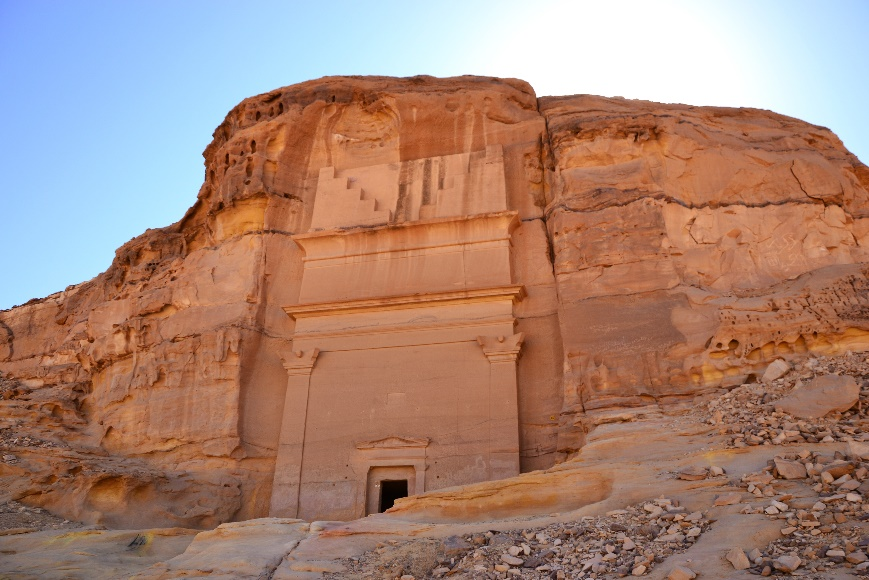
\includegraphics[width=3.94921in,height=2.63264in]{Images/image028.jpg}

Elle devient déserte à partir du IVe siècle et le Coran en donne la
raison~- Dieu a anéanti la ville, parce que ses habitants n'ont pas cru
aux prophètes~:

«~Certes, les Hommes d'al-Hijr ont traité les Envoyés d'imposteurs. Nous
leur avons apporté Nos signes et ils se sont détournés. Ils creusèrent,
tranquilles, des demeures dans les montagnes. Mais le Cri les prit au
matin, et à rien ne leur servit ce qu'ils possédaient~» (S. 15,
80-84)\sn{\textsuperscript{~}S.~15, 80-84 signifie que ce sont les
  versets 80 à 84 de la sourate 15\ldots{} on y reviendra dans le
  chapitre sur le Coran.}.


\begin{Synthesis}
Le Coran donne des informations
historiques, sur des épisodes passés, mais aussi sur l'histoire à
venir~. Mais il donne
surtout une lecture théologique de l'histoire.
\end{Synthesis}

Notons aussi l'existence de villes. \mn{La ville de Najran avait un évêque qui était probablement rattaché à l'église d'Éthiopie. Dhu Nuwas haïssait les chrétiens et faisait sans cesse la guerre au roi d'Éthiopie. Vaincu et forcé de payer tribut à Elesbaan, il se vengea sur les chrétiens de son royaume. Il agit par ruse : ayant rendu une visite protocolaire à la ville de Najran, il invita les notables à venir le voir dans son camp où ils furent tous capturés.   Devant leur refus de devenir juif, il
fait exécuter les 340 chrétiens de la ville, et décapiter le prince
Aréthas. Suite à ce massacre, le roi d'Ethiopie Elesbaan mena une
expédition punitive dans la cité, chassant Dounass, et rétablissant un
prince chrétien à la tête de la cité. Selon la plupart des commentateurs
du Coran, les hommes de Ukhdoud mentionnés au verset 4 de la sourate 85
ne seraient autres que les martyrs de Najran, tués et
brûlés.}Najrān est située en Arabie saoudite
à proximité du Yémen. Elle a été aussi capitale d'un petit royaume. Elle
était habitée par des juifs et des chrétiens. Un épisode terrible y a eu
lieu et est resté dans les esprits lorsque le roi juif Himyar en 523 a
fait assassiner des notables chrétiens.



Dans le Golfe et dans le Nord du Hijāz, les travaux archéologiques ont
mis en lumière des langues étrangères (akkadien, araméen, nabatéen,
grec, latin). Mais qu'en est-il de l'arabe comme idiome linguistique~?

\vide{lessor-de-la-langue-arabe}{%
\subsubsection{L'essor de la langue `arabe'
}\label{lessor-de-la-langue-arabe}}

Vous trouverez ci-dessous quelques éléments historiques sur l'essor de
la langue arabe. C'est un peu subtil tant dans les termes que dans la
géographie, à moins que vous ne soyez déjà un peu familier avec ce
monde. Dites-vous que ces informations ne sont pas là pour faire savant.
Il faut bien voir que de cette histoire linguistique nous pouvons
retirer des informations précieuses dans notre compréhension de l'islam
et de ses fondations puisque le Coran a été transmis justement \emph{en
arabe}~: Il le dit d'ailleurs de lui-même~: «~Un Coran \emph{en arabe}
pour les gens qui savent~» (S. 41,3). Donc\ldots{}

À l'époque antique, il existait au sein de «~l'Arabie heureuse~»
(c'est-à-dire le Yémen) quatre groupes lexicaux~: le sabéen, le
qatabānite, le ḥaḍramawtique et le madhābien. L'unification au IIIème
siècle de notre ère s'est traduite par la prédominance du sabéen. Il est
proche de l'arabe, mais il n'est pas l'arabe. L'arabe avec son article
«~al~» qui le caractérise se trouve dans une dédicace datant du IIème et
IVème siècle~: on trouve \emph{l-lt} (pour \emph{li-llât}) {[}pour
Dieu{]}. C'est écrit en alphabet sabéen, mais c'est de l'arabe~!

Au VI\textsuperscript{ème} siècle, il y a un lien entre la langue arabe
et l'écriture. Ce n'est pas l'écriture telle que nous la connaissons
aujourd'hui, mais c'est son ancêtre. C'est du vieil arabe. Le premier
témoignage de cette écriture est une inscription qui date de 512~: il
s'agit d'une dédicace à St Serge~à Zabad au sud d'Alep :

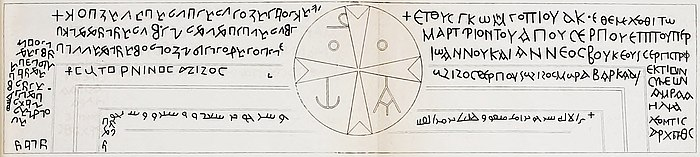
\includegraphics[width=5.51181in,height=1.23542in]{Images/image029.jpg}

autrement dit, l'écriture arabe a été utilisée par les chrétiens. Ce qui
est intéressant, c'est que l'inscription est en trois langues~: grec,
syriaque et arabe. On trouve une inscription à 100 km de Damas au roi
al-Harith datant de 538\emph{,} une inscription au sud de Damas datant
de 568, pour commémorer la construction d'un \emph{martyrum}. Qu'en
déduire~?

\begin{itemize}
\item
  On note que les premières écritures arabes sont en dehors de l'Arabie,
  ce qui plaide pour une influence syriaque dans l'émergence de l'arabe.
\item
  D'autres plaident pour une influence de l'alphabet
  nabatéen\sn{Pour rappel, les Nabatéens sont un peuple commerçant
    de l'Antiquité vivant au sud de la Jordanie et de Canaan, et au nord
    de l'actuelle Arabie. Vous avez entendu parler de Pétra~? Vous y
    êtes peut-être allés, dans ce cas vous savez déjà tout. Si vous ne
    savez pas ou si vous avez oublié, sachez que Pétra était la capitale
    de la Nabatène. Lieu magnifique. Tombé dans l'oubli, le site a été
    redécouvert en 1812 par un explorateur suisse,
    \url{http://www.hls-dhs-dss.ch/textes/f/F17075.php}{Jean-Louis
    Burckhardt} \ldots{} Une petite vidéo du ministère du tourisme
    jordanien vous donnera envie d'aller découvrir son `mystère'.
    \url{https://www.youtube.com/watch?v=YKk-JGeU_yY}{C'est ici~!}}.
\item
  En tous les cas, il semble que les premiers à parler arabe, n'étaient
  pas les Arabes. Et d'ailleurs qui sont ceux que l'on appelle Arabes~?
  Il est frappant de constater à partir des sources non musulmanes que
  ceux qui dirigent les «~conquêtes arabes~» au lendemain de la mort de
  Muḥammad ne sont pas appelés «~arabes~». On trouve les termes grecs de
  \emph{Sarakenoi} (Sarrasins), de \emph{Tayyayê'} dans les textes
  syriaques (du nom d'une tribu de l'Arabie du Nord-Est), de
  \emph{Haragènes}, de «~\emph{fils d'Ismaël}~» ou encore de
  \emph{magaritai} dans un papyrus daté de 643 ou de
  \emph{maghrâyê}\sn{Françoise \textsc{Micheau}, \emph{Les débuts
    de l'islam}, Paris, Téraèdre, 2012, p. 52.}.
\end{itemize}

La première mention du mot `arabe' se trouve sur une inscription
assyrienne~; elle date de 853 avant JC. Il y est question de la mention
d'adversaires et notamment Gindibu' l'Arabe. Plus tard, le terme
apparaît pour désigner des peuplades nomades, avec leurs chameaux.

\foreignlanguage{greek}{
Ἰουδαῖοί τε καὶ προσήλυτοι, Κρῆτες καὶ Ἄραβες, ἀκούομεν
λαλούντων αὐτῶν ταῖς ἡμετέραις γλώσσαις τὰ μεγαλεῖα τοῦ θεοῦ.} (Ac 2, la
Pentecôte)



Cela ne se limite pas à la péninsule de l'Arabie\ldots{} on désigne
aussi par Arabe ceux qui vivent au bord du Nil. On en a un bel exemple
chez Hérodote. Le terme est donc en premier lieu \textbf{employé par
l'extérieur pour désigner ces populations}. La première fois qu'elles
parlent d'elles-mêmes en se désignant par ce mot, se voit sur une
inscription du 3\textsuperscript{ème} siècle de notre ère où un individu
dit de lui qu'il est \emph{`arabī}. Il y a une inscription du
4\textsuperscript{ème} siècle, où il est question d'un groupe d'arabes.

\begin{itemize}
\item
  À la veille de l'islam, il y a donc un ensemble vaste de populations
  qui ne se désignaient pas eux-mêmes ou rarement par le terme d'arabe.
\end{itemize}

\textbf{Du coup, on se demande s'il ne s'agit pas d'une construction
\emph{a posteriori}.}

\vide{lenvironnement-religieux-de-la-puxe9ninsule-arabe}{%
\subsection{{L'environnement religieux de la
péninsule arabe
}}\label{lenvironnement-religieux-de-la-puxe9ninsule-arabe}}

Nous avons vu que La Mecque abritait un temple aux multiples divinités.
Nous avons vu aussi que des chrétiens et des juifs s'y trouvaient. Au
regard de l'histoire des royaumes voisins, il n'y a rien de surprenant.
Mais entrons un peu plus dans le détail\sn{Dans un souci
  synthétique, je m'appuie notamment sur une contribution très bien
  faite de Michel Reeber, «~Le contexte religieux de l'Arabie
  préislamique~», dans \emph{Le Coran et la Bible}, Paris, 2002, p.
  13-42.}.

\vide{le-polythuxe9isme-de-larabie-le-culte-buxe9tylique}{%
\subsubsection{{Le polythéisme de l'Arabie~: le
culte bétylique
}}\label{le-polythuxe9isme-de-larabie-le-culte-buxe9tylique}}

Si vous avez eu la curiosité de lire l'article de Jacqueline Chabbi,
vous vous souvenez probablement que les Bédouins pratiquaient le culte
des bétyles, c'est-à-dire ces roches sacrées censées être la demeure
d'un dieu (bétyle vient de \emph{bayt} -- maison et de \emph{el} -
dieu). Les pierres étaient transportées par les tribus nomades, mais à
La Mecque, cité sédentaire, on avait édifié un temple qui les abritait.
La fameuse pierre noire qui est dans l'actuelle Ka`ba n'est pas sans
rappeler cette tradition bédouine. Elle a donné lieu à de multiples
légendes. L'une d'entre elles dit qu'elle fut jetée du ciel sur terre et
que blanche elle était, mais que ce sont les péchés des hommes qui l'ont
rendue noire. Cela me rappelle une tradition chrétienne antique à propos
du baptême de Jésus~: on a pu dire que Jésus immaculé, donc de blanc
qu'il était, au moment de son baptême est ressorti noir du Jourdain car
il portait le péché des hommes\ldots{}

Il existait aussi des rituels de circumambulation autour de la Ka`ba
ainsi qu'un pèlerinage entre Marwa et Safa, le jet de pierres autour
d'une stèle, la vénération de feux sacrés. L'islam, comme nous le
verrons, garde souvent une emprunte de ces rituels, mais il les a
islamisés. En revanche, pas de feu. \textbf{Le passage au calendrier
lunaire a permis de maintenir des pratiques tout en rompant avec les
rituels solaires liés aux saisons, marquant ainsi une vraie rupture avec
les rites antéislamiques.}

Parmi les rites, on offrait aussi des sacrifices d'animaux ou même
d'êtres humains. Le Coran fait mention des sacrifices d'enfants qui
semblent être courants~:
\begin{quote}
S. 6, 137~: «~Et c'est ainsi que leurs divinités ont enjolivé à beaucoup
d'associateurs le meurtre de leurs enfants, afin de les ruiner et de
travestir à leurs yeux leur religion. Or si Allah voulait, ils ne le
feraient pas. Laisse-les donc, ainsi que ce qu'ils inventent~».
    
\end{quote}

  Ce verset pointe une pratique, mais en même temps, il est ambigu
  puisque\textbf{,} s'il montre l'horreur du massacre et ses
  conséquences funestes\textbf{,} il n'invite pas pour autant à lutter
  contre ces pratiques, comme si elles étaient voulues par Dieu et
  conduisaient \emph{in fine} à la mort des idolâtres.

Quant au Panthéon, s'il y avait plusieurs dieux, le culte de Hubal, qui
provient de Mésopotamie ou de Syrie, était prédominant\sn{Toufic
  Fahd, Le Panthéon de l'Arabie Centrale à la veille de l'Hégire,
  Institut Français d'Archéologie de Beyrouth : Bibliothèque
  archéologique et historique, n°88, 1968.}. Une statue dans le Temple
de la Ka`ba le représentait.


\paragraph{Houbal}{Divinité principale du panthéon arabe,
Houbal était connu sous le nom de « Seigneur de la Ka'ba ». Il était
probablement le père de la Triade des déesses Allât, Al-'Uzzâ et Manât,
les Filles de Houbal. En dehors de l'Arabie du sud, son nom apparaît
seulement dans une inscription nabatéenne où il est associé à deux
autres divinités, Dhu-al-Sharâ (Dusarès ; en arabe : \TArabe{ ذو الشّرى }et
Manawatu (en arabe :\TArabe{ مناة-مناواتو,} équivalent arabe nabatéen de Manât).;
'après Ibn Ishaq, la statue de la Ka'aba était une effigie
anthropomorphe en cornaline ; la Sira rapporte qu'Abd al-Muttalib ayant
promis un fils en sacrifice à Houbal qui l'avait aidé à retrouver la
source Zamzam, le sort aurait tout d'abord désigné Abdallah, père de
Mahomet. Sur les conseils d'une devineresse, on aurait proposé au dieu
cent chameaux en échange. Après dix divinations, chacune suivie d'une
augmentation du nombre des chameaux, Abdallah eut la vie sauve contre
mille chameaux.
}

\paragraph{Trois divinités} le concurrençaient. Comme nous l'avons vu, elles sont
mentionnées dans le Coran~: al-Uzzā, al-Lāt et Manāt (S. 53, 19-20).
Al-Uzzā était la déesse vénérée par les Quraysh, tribu dont est issu
Muḥammad. Selon les historiens musulmans, la Ka`ba contenait quelques
360 figurines (tiens, c'est la réponse à la question du
1\textsuperscript{er} chapitre). Muḥammad, de retour à La Mecque après
son Hégire à Médine, donnera l'assaut contre elles et les détruira
toutes, à l'exception de deux d'entre elles. \textbf{Quelles sont ces
fameuses deux icônes qu'il n'a pas fait
détruire}\sn{D'après la tradition, Mahomet, lorsqu'il investit la
  Kaaba, ordonna la destruction de toutes les idoles, sauf une : une
  icône mariale qu'il protégea de ses mains. Maryam, mère du prophète
  Jésus, Isâ (Issa), est donc vénérée partout par les musulmans.}\textbf{\ldots{}
Ce n'est pas sans incidences sur la nature des relations entre
communautés de religions différentes, ni non plus sans conséquences
aujourd'hui.} On en reparlera.

La connaissance de cette culture religieuse tribale permet d'enraciner
la compréhension de l'islam et notamment de ses rites. Mais plus encore,
elle permet de comprendre le Coran lui-même. C'est le propos de la
recherche de Jacqueline Chabbi dans son ouvrage \emph{Le Coran
décrypté}. Elle montre que certains passages s'éclairent en lien avec le
milieu tribal de Muḥammad. Ainsi, par exemple, elle remarque que bien
des métaphores eschatologiques et bibliques du Coran sont une réécriture
adaptée à la culture tribale. À cet égard, il est symptomatique que le
paradis soit décrit comme une oasis, un jardin (\emph{ğanna}) irrigué de
canaux toujours à ras bord (\emph{anḥār}), ombragés et sans soleil
(\emph{lā yarawna fihā `amsan}) (S. 76, 13)\sn{~Jacqueline Chabbi,
  «~La possibilité du Coran comme document anthropologique~», dans Mehdi
  \textsc{Azaiez} (dir.) et Sabrina \textsc{Mervin} (coll.), \emph{Le
  Coran}. Nouvelles approches, CNRS Editions, 2013, p. 189-205.}. On est
ici en plein milieu culturel arabe caractérisé par une phobie du soleil.
Ce travail sur le milieu tribal de l'Arabie antéislamique n'est pas sans
incidence dans la compréhension du Coran mais aussi dans ses
traductions. Ainsi, par exemple, la traduction de \emph{anḥār} par
fleuves, comme pour les fleuves bibliques du paradis, est un \emph{a
priori} de traduction et ne rend pas compte de sa signification exacte.
Il n'y a pas de fleuves, ni de rivières dans la péninsule arabe, juste
des points d'eau, quelques sources, parfois des lacs souterrains à
l'instar de La Mecque. De la même manière, la représentation de l'enfer
dans le Coran s'appuie sur le milieu tribal. Il est question du
\emph{ḥamīm} (S. 47, 15)~: c'est la pluie des orages d'été~; c'est lui
qui vient abreuver les damnés. Ils n'ont pour seule nourriture que le
\emph{dari'}, c'est-à-dire l'herbe à chameaux. Le \emph{nār,} traduit
par enfer, \ldots{} est en fait un feu solaire perpétuel.

Dans son dernier livre, \emph{Les trois piliers de l'islam}, elle montre
que l'islam tel qu'il se construit au cours de l'histoire est
essentiellement une construction à l'époque abbasside, époque
caractérisée par des guerres avec l'empire byzantin~; époque qui est
aussi celle d'un empire qui cherche à se démarquer de la première
dynastie des Omeyyades, époque où les textes sont fixés et notamment les
recueils de \emph{Sunna}. Or, les recenseurs ne sont pas arabes. Ils
proviennent de milieux culturels de contrées lointaines à l'Arabie~:
Buḫārī est de Transoxiane (actuel Ouzbékistan), Muslim de Nišapūr
(actuel Nors-Est de l'Iran), etc. quant à la \emph{Sunna} d'Ibn Ḥanbal,
le maître bagdadien, sa \emph{Sunna} ne fait pas partie des livres
canoniques\sn{Chabbi, Jacqueline,~\emph{Les Trois Piliers de
  l'islam}, \emph{op.cit.}, p. 15.}. Or, \textbf{leurs lectures, dans la
mesure où la Sunna est aussi l'herméneutique du Coran, vont imposer une
compréhension du Coran qui se détache du sens du Coran des origines.}
Pour l'historienne, il ne s'agit pas de rejeter ces lectures -- cela
relève de la démarche théologique, croyante -- mais de dire qu'une
attention à l'anthropologie du milieu où est prêché le Coran donne des
clefs de compréhension au texte sacré de l'islam. Pour autant, on peut
dire que Chabbi voit dans ce travail une mission salutaire~: c'est ici
que l'historienne se fait engagée~: à l'heure du fondamentalisme où des
idéologies se vantent de revenir au sens originel, il s'agit de lire le
Coran dans toute la vigueur de son verbe au-delà des lectures qui lui
furent accolées et qui lui sont encore posées.
\begin{quote}
    «~Ils lisent certes mais, ne connaissant ni les tenants ni les
aboutissants du texte, que comprennent-ils~? Texte sans contexte et sans
rattachement à un passé et à une tradition n'est que ruine du sens,
pourrait-on dire en plagiant un célèbre aphorisme~» (p.~31-32).
\end{quote}


Mais quel est ce sens originel du Coran ? Et comment le retrouver~?

L'auteur reconnaît qu'il sera difficile, voire impossible, de le
ressusciter car il prend naissance au sein d'une culture de l'oralité~;
il y a donc un «~écart sociologique~» (p.~11). Cependant, le Coran
témoigne de l'importance du milieu anthropologique, et si les références
bibliques restent parfois évasives, ce n'est pas parce qu'elles sont
connues -- ce que soutient Guillaume Dye -- mais parce qu'elles sont
réinterprétées. Or, le milieu anthropologique de l'Arabie est celui de
la culture tribale marquée par trois piliers~: \textbf{l'alliance, la
guidance et le don}. Ces piliers sont de nécessité pour les hommes de ce
milieu. Ils se retrouvent dans le Coran et doivent être abordés à partir
des sens qu'ils avaient à l'époque. Son étude lexicale lui permet aussi
d'identifier l'hétérogénéité des champs lexicaux en fonction des milieux
mecquois et médinois~: ainsi, elle remarque que le vocabulaire à Médine
y est beaucoup plus diversifié, et l'influence de l'hébreu y est plus
net. La terminologie y est aussi renouvelée. Symptomatique à cet égard
est la racine \emph{baraʾ} pour désigner la création~: si elle se trouve
au livre de la Genèse, elle est absente des versets mecquois. Plus
largement, Chabbi replace le sens du mot \emph{kitāb} -- traduit
communément par «~livre~» -- au sein de la culture de l'oralité~: il ne
s'agit pas d'un livre matériel, mais d'un message fixé oralement
(p.~58). L'univers tribal s'exprime aussi dans la nature des
descriptions eschatologiques. Ces croyances sont nouvelles et
constituent une nouveauté pour les mecquois, mais elles déploient un
code symbolique relatif au désert~qu'il s'agisse de la tempête ou du
combat contre une tribu.

Sur la nature religieuse du milieu de la péninsule arabique, elle
souligne qu'il est avant tout marqué -- et plus \textbf{à La Mecque qu'à
Médine -- par le caractère bétylique \mn{p.~117}. À cet égard, le mot
\emph{bayt} dans le Coran ne renvoie pas à un temple ou à une maison,
mais au cœur de la cité mecquoise, la Kaʿba~}: il existe une symétrie
entre la demeure de la divinité et celle des hommes puisqu'il s'agit
d'un modèle de duplication appliquée à la divinité censée les
\textbf{protéger} (p. 117).

Quant à la question des prophètes mentionnés dans le Coran, ils ont fait
l'objet d'une étude approfondie par l'islamologie\sn{~Speyer,
  Heinrich, \emph{Die Biblischen Erzählungen im Qoran,} Hildesheim, G.
  Olms, 1961 (1931).}. L'originalité de la recherche de Chabbi est de
montrer que les thèmes qui leur sont rattachés sont adaptés au monde
tribal. Ainsi, à propos de la confrontation d'Abraham avec des idoles
(\emph{asnām}), on a généralement mis en avant le rapprochement de ce
texte coranique avec le chapitre 12 du \emph{Livre des
Jubilés}\sn{Voir pour le Testament d'Abraham~: Gobillot,
  Geneviève, «~Le Coran, guide de lecture de la Bible et des textes
  apocryphes~», \emph{Pardès} 50, 2, 2011, p. 131-154.}~mais, pour
Chabbi, le cœur du message ne porte pas tant sur les pierres taillées
que sur l'opposition entre la croyance des pères (\emph{ābāʾ}) et celle
qu'il faut désormais accorder au Seigneur des peuples/tribus (\emph{Rabb
al-ʿālamīn}) (p. 97) -- non pas «~Seigneur des mondes~» selon la
traduction commune mais «~Seigneur des tribus~» --. Par conséquent, Dieu
est celui qui crée, guide, nourrit, abreuve, fait mourir et revivre. Le
Seigneur vient se substituer aux dieux incapables de protéger et de se
protéger (Cor.~26,~92-93). Dans la péninsule arabique, le \emph{Rabb},
est une figure protectrice.

 
\mn{\url{https://fr.wikipedia.org/wiki/Ar-Rahman}} 


\paragraph{Raḥmān}
L'évolution sémantique pour désigner Dieu est dans le Coran hautement
illustrative du thème de l'alliance. Ainsi, \textbf{la figure de
\emph{Raḥmān}},\TArabe{ الرحمن } \emph{le miséricordieux}~ \textbf{est propre à la
période mecquoise et disparaît au temps de Médine pour être remplacée
par celle d'\emph{Allāh}}. La notion de \emph{Rabb} renvoie à l'idée
d'un échange~; il y a une personnalisation de la relation par
l'expression \emph{Rabbī}, mon Seigneur (p. 143). Le divin est
foncièrement le \emph{walī}, c'est-à-dire le proche, le
\textbf{{protecteur}}.

Le \emph{muʾmin}\sn{(\textsc{a}.), participe actif de la
  4\textsuperscript{e}~forme de la racine~\emph{ʾmn}, signifie
  «Croyant», mais est aussi l'un des noms de Dieu (LIX, 23).}, n'est pas
d'abord celui qui croit, mais celui qui s'est rallié avec confiance.
Chabbi écrit~:
\begin{quote}
    
«~L'importance des occurrences de cette terminologie est frappante. Elle
témoigne de la spécificité de l'engagement mutuel du divin et de
l'humain, car l'alliance n'est jamais gratuite~; elle ne va pas sans
contrepartie de part et d'autre~» (p.~153).
\end{quote}
\begin{Ex}

{Quand on parle de Rahman avec un musulman, miséricorde
n'a pas forcément le même sens~: pardon pour un chrétien, bienfaisance
(pluie) pour un
musulman}
\end{Ex}

Quant au nom \emph{Rahmān}, elle remarque que si la racine hébraïque
connote l'idée de compassion et de miséricorde, sa réappropriation dans
le milieu tribal via le monde yéménite le connote de l'idée de
bienfaisance et de bienveillance. Le \emph{Rahmān} joue le rôle du Dieu
qui dispense la pluie, fonction établie à Athtar, dieu de la pluie du
Yémen (p.~127). Mais la tradition musulmane dit-elle autre chose~? Il
est frappant de constater que les traités théologiques musulmans sur les
noms divins s'inscrivent pleinement dans la définition d'une
\emph{raḥma} comprise non comme miséricorde au sens chrétien, mais
bienveillance et bienfaisance, à l'instar de celui d'al-Ġazālī \label{theol:AlGazali23}. Sur ce
point, Chabbi vient davantage corriger une traductologie influencée par
le vocabulaire théologique du christianisme que renouveler le sens
terminologique au sein de la tradition islamique.

\vide{alliance}{%
\subsubsection{Alliance}\label{alliance}}

Du point de vue du développement des idées religieuses, Chabbi souligne
l'émergence du allāhisme, mouvement de ralliement à une divinité qui
assume les fonctions assignées aux divinités d'un milieu tribal~:
alliance et protection, jugement eschatologique. Au cours de la
révélation mecquoise, \emph{Ilāh} est d'abord le dieu qui s'impose sur
les autres dieux. La notion de \emph{\textbf{walāʾ}} , ô combien
utilisée dans les milieux fondamentalistes et salafistes d'aujourd'hui,
signifie \textbf{l'alliance, la solidarité} au sein d'un même groupe
partageant le même espace.

\vide{guidance}{%
\subsubsection{Guidance}\label{guidance}}

De même, les noms divins se comprennent dans le cadre du monde tribal~:
dire de Dieu qu'il est \emph{ʿalīm}, c'est faire de lui le maître des
signes (\emph{aʿlām}) et Chabbi de préciser que cela renvoie au signe de
la piste~: \emph{Ilāh} est celui qui guide et conduit. Il connaît
l'avenir et permet de guider son groupe afin de le protéger des périls.
Ce dont il protège ce n'est pas la nuit, mais la ténèbre -- nuit sans
lune où l'on ne peut plus suivre la piste -- alors que les nuits
éclairées par la lune rendent le chemin des caravaniers aisés par
contraste avec les chaleurs de la journée. Dans le désert, la guidance
(\emph{hudā}) est de nécessité~: elle est une question de vie ou de
mort. Et si Dieu guide, c'est pour protéger de la mort non pour inviter
à en prendre le chemin. Là encore, l'analyse se fait engagée~:
\begin{quote}
«~Autant dire que les outrances actuelles qui assurent préférer la mort
dans la voie de Dieu en croyant prendre appui sur le passé premier sont
en totale contradiction avec la parole coranique telle qu'elle
s'adressait aux hommes de son temps dans la société qui était la leur~»
(p.~157).
\end{quote}

Les routes sont des chemins dangereux, surchargés d'embûches physiques
et surnaturelles, de puissances hostiles si bien que tout déplacement
est une aventure périlleuse. Dans ce contexte, les dieux préislamiques
exerçaient la fonction de guide. Les seigneurs (\emph{arbāb}) n'étaient
pas les maîtres de ces lieux mais ils pouvaient y conduire les hommes et
les guider, les protéger. Or, le sédentaire, non habitué à se déplacer,
devait pour tout déplacement recourir à des guides. \textbf{La parole
coranique exprime ce besoin~: elle n'est pas issue d'un milieu nomade,
mais sédentaire.} La thématique de la guidance permet donc à l'auteur de
restituer le sens perdu de mots clefs du vocabulaire coranique et
islamique.

\vide{ux161arux12bux2bfa-voie}{%
\paragraph{šarīʿa~, voie}\label{ux161arux12bux2bfa-voie}}

Ainsi en est-il de \emph{šarīʿa}~: elle est la voie donnée pour éviter
de se perdre~: elle est grâce accordée à Muḥammad alors que les enfants
d'Israël se sont écartés du chemin, bien que Dieu les avait favorisés
(\emph{tafdīl}) (Cor.~45,~15-18). Cette voie renvoie à un point d'eau où
l'eau affleure, ce qui permet aux dromadaires de s'y désaltérer sans que
l'on doive aller y puiser~: c'est donc un lieu facile d'accès. Ainsi,
Dieu, par la \emph{šarīʿa}~donne accès à l'eau~; il dispose de
ressources qu'il partage. Par suite, perdre la voie conduit au malheur,
à l'exemple des fils d'Israël (Cor.~45, 17). En conclusion, Chabbi
remarque que le Coran est loin de la signification qui sera donnée à ce
terme et qui ne date que du iii\textsuperscript{e} siècle de l'Hégire
(p.~177). Elle conclut aussi que l'intégration de châtiments corporels à
la \emph{šarīʿa}~est impossible en milieu pré-islamique et se trouve aux
antipodes des solidarités qui s'y nouaient. La seule disposition légale
qui se retrouve dans le Coran est celle du \emph{qiṣāṣ}, le prix du sang
(Cor.~4, 92).

\vide{lapidation-mentionnuxe9e-dans-la-sira}{%
\subsubsection{Lapidation mentionnée dans la
sira~?}\label{lapidation-mentionnuxe9e-dans-la-sira}}

Quant à la lapidation (\emph{raǧm}), elle était pratiquée non pour tuer,
mais pour éloigner l'indésirable à l'exemple des puissances maléfiques
dont il s'agit de se prémunir pour éviter de subir leur malfaisance (p.
178) (Cor. 86, 25~; Cor. 15, 17, 34).

\vide{la-sunna-la-piste-sure}{%
\paragraph{La sunna, la piste sure}\label{la-sunna-la-piste-sure}}

De même, si le mot \emph{Sunna} désigne la piste sûre, réputée,
attribuée à Dieu, la \emph{Sunna d'Allāh} est une voie de châtiment pour
ceux qui ont trahi l'alliance. Elle n'est pas un modèle à suivre, sens
qui sera donné à propos de Muḥammad. Cette expression, typique du
sunnisme, a cherché à se fonder sur le Coran à partir du mot
\emph{uswa}, se rallier à\emph{.} Ainsi, Abraham a-t-il été présenté
comme un exemple à suivre en tant qu'il a rompu avec l'allégeance des
dieux de ses pères (Cor. 60, 4 et 6). De même, le messager d'Allāh
(désigné comme Muḥammad par les commentateurs) est-il présenté comme un
exemple à suivre (S.~33, 21). Mais pour Chabbi, le contexte n'est pas
celui du modèle, mais de l'alliance~: il est celui qui s'est rallié à
Dieu. La \textbf{Sunna de Dieu renvoie donc à une coutume divine~qui
consiste à rejeter, à faire disparaître celui qui s'éloigne ou qui
accuse le messager de Dieu de mensonge.}

À propos du terme \emph{umma}, communément traduit par «~communauté~»,
Chabbi souligne que dans le Coran, là aussi, il désigne la bonne voie :
«~Nous avons trouvé nos pères sur une \emph{umma} et c'est assurément
leurs traces qui nous sont modèle {[}pour suivre la route{]} \emph{ʿalā
aṯāri-him muqtadūn}~» (Cor. 43, 22). Quant au \emph{ǧihād}, si on a
souligné à maintes reprises qu'il est un effort, Chabbi resitue cet
effort par rapport au milieu local où le sédentaire est désigné comme
celui qui reste sur place (p. 194). Dans un monde où la chaleur brûle
les corps, tout déplacement est un enfer. Face à la tentation de
s'installer, le Coran affirme que le paradis leur sera interdit.
\textbf{Aussi, l'image du paradis renvoie-t-elle à un monde immobile,
sans activité.} Il est la récompense accordée à la suite de à l'effort
engagé dans les pas de Muḥammad. D'où les images eschatologiques comme
celles de l'accoudement (\emph{ittikāʾ}). «~Le paradis coranique semble
ainsi avoir horreur du mouvement. Il fige les élus dans l'immobilité
d'un repos qui les fait en quelque sorte échapper à la course harassante
pour la vie qui avait été leur lot durant leur vie~» (p. 293).

\vide{ux1e7ihux101d-combat-pour-la-voie-dallux101h-dans-un-monde-ouxf9-le-paradis-est-limmobilituxe9}{%
\paragraph{Ǧihād, combat pour la voie d'Allāh dans un monde où le
paradis est
l'immobilité}\label{ux1e7ihux101d-combat-pour-la-voie-dallux101h-dans-un-monde-ouxf9-le-paradis-est-limmobilituxe9}}

Le \emph{ǧihād} devient le combat à mener dans la voie d'Allāh, il est
le \emph{qitāl}. Et traduire \emph{qitāl} par le fait de tuer est une
altération de sens car il ne s'agit pas de tuer pour tuer, mais il
s'agit de combattre en sachant que ce combat peut conduire à la mort (p.
200-201). Mais «~tuer les hommes d'un groupe adverse de manière
inconsidérée ou gratuitement massacreuse constitue une transgression
majeure~» (p. 203).


\mn{Combien est vil le prix contre lequel ils ont troqué
leurs âmes lorsqu'ils ont nié ce que Dieu a révélé et ce, uniquement par
dépit, car ils n'ont pu admettre que Dieu, par un effet de Sa grâce, ait
choisi certains de Ses serviteurs pour les gratifier de la révélation !
Ils se sont ainsi attirés doublement la colère du Seigneur et le
châtiment ignominieux qui sera réservé aux
infidèles.}



Le verset Cor. 2, 90 rappelle à cet égard qu'il ne faut pas commettre
d'agression (inconsidérée), que Dieu n'aime pas les agresseurs
(\emph{muʿtadīn}).

Par opposition, la négociation qui permet de répondre au risque encouru
est considérée comme un don (\emph{fatḥ}). Le chapitre consacré à la
violence permet ainsi de rappeler que dans tous les cas, l'action de la
violence revient à la divinité. L'exacerbation de la parole coranique
doit être lue comme la conséquence de l'immobilisme des hommes. À
Médine, le prophète réclame l'obéissance (\emph{tāʿa})~; il y a ici une
rupture avec La Mecque où le Coran orientait sur l'obéissance à la
divinité.

\begin{table}[h!]
    \centering
    \small
   \begin{tabular}{p{0.45\textwidth}p{0.45\textwidth} }
À l'expiration des mois sacrés, tuez les polythéistes partout où vous
les trouverez ! Capturez-les ! Assiégez-les ! Dressez-leur des
embuscades ! S'ils se repentent, s'ils accomplissent la salât, s'ils
s'acquittent de la zakât, laissez-les en paix, car Dieu est Clément et
Miséricordieux. & Faitha insalakha alashhuru alhurumu faoqtuloo
almushrikeena haythu wajadtumoohum wakhuthoohum waohsuroohum waoqAAudoo
lahum kulla marsadin fain taboo waaqamoo alssalata waatawoo alzzakata
fakhalloo sabeelahum inna Allaha ghafoorun raheemun (⁎) \\
 
\end{tabular}
\sidecaption{verset dit du sabre (Cor. 9, 5)}
\end{table}

À propos du verset dit du sabre (Cor. 9, 5), la précision temporelle
«~après les mois sacrés~», montre une mise en conformité avec les règles
tribales (p.~249). L'injonction «~tuez-les~» est incompatible avec le
contexte du verset qui invite à accueillir les repentants~: il s'agit
donc d'abord de combattre~; par ailleurs cet appel est une réponse à une
agression antérieure.

\vide{don}{%
\subsubsection{Don}\label{don}}

Enfin, concernant le don, il est mutuel (p.~265). Conformément à ce
qu'avait montré Mauss, celui qui ne peut donner est dans une situation
très faible car \textbf{le don est aussi une marque de pouvoir}. Par
conséquent, \textbf{l'orphelin} a la position la plus inférieure. Dans
la logique du don coranique, il s'agit de donner, mais sans s'appauvrir
soi-même. Pour autant, le don appelle le contre don et Chabbi propose
une interprétation très intéressante du \emph{\textbf{kufr}} traduit
habituellement par \textbf{infidélité} ou mécréance. Pour elle, il
désigne \textbf{l'ingratitude}~: «~ce serait un moyen de se soustraire à
une obligation sociale en masquant la bienfaisance dont on a été
bénéficiaire~» (p.~266). La thématique du don divin est typiquement
tribale. Les délices du paradis, le repos eschatologique, sont la
récompense de la divinité à celui qui se sera investi dans ce monde et
aura su répondre à ses obligations. Mais le don n'est pas seulement lié
au futur. Dès ici-bas, la divinité offre~: ce sont les dons de
subsistance. Dieu est celui qui offre ces pâturages verdoyants, et parmi
les traductions originales avancées dans l'ouvrage, pour Chabbi,
traduire le verset Cor. 16, 80 par «~peut-être deviendrez-vous
musulmans~» est un anachronisme~: dans le contexte tribal, il s'agit
d'accepter de se mettre sous la garde de la divinité qui assure ces
bienfaits. Chabbi propose~: «~peut-être accepterez-vous de vous mettre
sous sa garde {[}dans la mesure où son alliance vous apporte tant
d'avantage en natures{]}~» (p. 330).

\vide{le-judauxefsme-dans-larabie-pruxe9islamique}{%
\paragraph{1.2.2 Le judaïsme dans l'Arabie
préislamique}\label{le-judauxefsme-dans-larabie-pruxe9islamique}}

À la suite de la destruction du Temple en 70, d'importantes communautés
juives émigrèrent au Moyen-Orient, en Babylonie, en Égypte, en Afrique
du Nord, à Byzance, en Italie. Certains juifs ont aussi émigré dans le
Hijāz (Arabie). La Mishna (compilation des enseignements de la loi
juive) rédigée en 200-220, en fait mention. On a pu identifier la
présence d'une vingtaine de tribus juives.

Il existait aussi une importante communauté juive dans le sud de la
péninsule arabique (Yémen). Les rois de Himyar ont fait le choix de
rejeter le polythéisme et après 380 on ne trouve plus dans tout le Yémen
la moindre inscription explicitement païenne. Cette rupture est très
profonde et se voit dans le vocabulaire avec l'usage d'une terminologie
araméenne et hébraïque comme \emph{amen}, `\emph{ālam} (monde),
\emph{bâraka} (bénir), \emph{shalôm}, \emph{salāt} (prière),
\emph{zakât} (grâce). Au début du VIème siècle, le judaïsme est la
religion dominante dans le royaume de Himyar\sn{Iwona Gajda, Le
  royaume de Himyar à l'époque monothéiste -- L'histoire de l'Arabie du
  Sud ancienne de la fin du IVe siècle de l'ère chrétienne jusqu'à
  l'avènement de l'islam.}. Avec l'unification de l'Arabie méridionale,
au 3\textsuperscript{ème} siècle, les rois de Himyar interviennent dans
l'Arabie désertique.

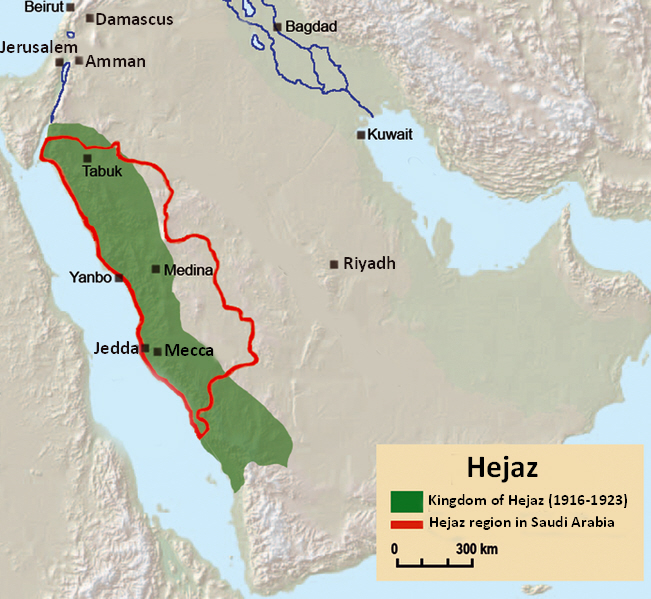
\includegraphics[width=\textwidth]{Images/image030.jpg}

Si globalement les juifs \mn{pour plus de détail sur le rapport entre Islam et judaisme, voir \cite{BarAsher:JuifsCoran}} refusèrent de se convertir à l'islam,
l'historiographie musulmane retient la conversion de certains d'entre
eux. Le plus connu est `Abd Allāh Ibn Salām, docteur de la Loi juive. Il
contribua à prêcher la conformité de la venue de Muḥammad avec la Torah.
Il est important de voir que ces premiers convertis apportent avec eux
leur culture biblique. Cela leur sera d'ailleurs reproché, comme ce fut
le cas pour un autre rabbin, Ka'b al-Akhbār. Retenez bien ce point quand
on parlera du Coran et de sa rhétorique~\ldots{} qui est très sémite.
Mais ces juifs qui fréquentent Muḥammad ou qui se convertissent dans les
premières décennies de l'islam, qui sont-ils exactement~? À quel courant
du judaïsme les rattacher~? De ce que le Coran rapporte concernant leurs
croyances sur Dieu, les anges, la création, la loi, le péché,
l'eschatologie, il semble que l'on puisse voir un lien de filiation avec
le judaïsme talmudique. Certains y ont vu des hétérodoxes juifs, mais
l'orientaliste Geiger\sn{A. \textsc{Geiger}, \emph{Was hat
  Mohammed aus dem Judenthum aufgenommen}, Bonn, 1833.}, à la lumière du
caractère sommaire des croyances juives telles qu'elles sont rapportées
par Muḥammad, suggère plutôt que les informateurs juifs de Muḥammad
étaient ignorants de leurs propres traditions -- autrement dit, il nous
invite à ne pas réduire le judaïsme de l'époque à ce que les
informateurs ont dû en rapporter. Cela rappelle un prisme méthodologique
dénoncé par al-Ġazālī \label{theol:AlGazali24} dans le \emph{Munqiḏ min al-ḍalāl} et que nous
avons vu dans la leçon précédente. Si vous avez oublié, relisez~:
\textbf{al-Ġazālī vérifie ce qu'il a compris d'une croyance auprès
d'autres membres de cette croyance.}

À La Mecque (lieu où commence la prédication de Muḥammad en 610), il est
difficile d'évaluer l'importance de la communauté juive. Mais les
versets coraniques révélés dans cette première période témoignent de
relations positives et fructueuses. La direction de la prière est
Jérusalem, le jour du jeûne (\emph{`ashūrā'}) rappelle le Yôm Kippour,
et le Coran reconnaît l'élection des juifs.
\begin{quote}
    «~Ô enfants d'Israël, souvenez-vous des bienfaits dont je vous ai
comblés~: souvenez-vous que je vous ai élevés au-dessus de tous les
humains~» (S. 2, 46).
\end{quote}


Mais à Yathrib (Médine), les juifs étaient plus nombreux.

Médine est située à 350 km de La Mecque. C'est une oasis. Il y avait une
école où l'on apprenait l'hébreu. Un des secrétaires de Muḥammad qui
sera chargé de collecter les sourates, Zayd Ibn Thābit, aurait fréquenté
cette école. En 622, au moment où Muḥammad doit fuir La Mecque et où il
va s'installer à Médine, il y a trois grandes tribus juives~: les Banū
Qurayẓa, les Banū al-Nadhîr et les Banū Qaynukā'. Ils avaient en leur
possession des terres riches et détenaient le pouvoir local. Peu à peu,
leur puissance déclina avec l'arrivée de deux tribus arabes, les Aws et
les Khazraj.

Il semble que les relations entre Muḥammad et les juifs de Médine furent
bonnes à son arrivée. Un document, «~La charte de Médine~» semble aller
dans ce sens.

\vide{clauses-en-rapport-avec-les-musulmans-et-les-croyants-monothuxe9istes}{%
\subsubsection{Clauses en rapport avec les musulmans et les croyants
monothéistes}\label{clauses-en-rapport-avec-les-musulmans-et-les-croyants-monothuxe9istes}}
\begin{quote}
 
 
 
{Les émigrés Qoraïchites et de Yathrib (Médine) et ceux
qui les suivirent et luttèrent avec eux forment une seule communauté à
part. Tous les musulmans quelles que soient leurs tribus ou
clans partagent entre eux le prix du sang, payent la rançon des captifs
selon le bon usage et
l'équité.
Les croyants monothéistes ne délaissent jamais un endetté
qui a la charge d'une famille ; ils lui donnent des fonds destiné à
payer le prix du sang ou le rachat d'un
captif.Tous les croyants monothéistes devront s'unir contre
quiconque étant rebelle ou cherchant à promouvoir l'hostilité ou la
sédition, quels que soient leurs liens familiaux ou
tribaux.  Aucun croyant monothéiste ne doit en tuer un autre, ou
soutenir un non croyant au détriment d'un
croyant.La protection de Dieu est sur tous les croyants
monothéistes, indépendamment de leur classe ou de leur origine
tribale.} 
 
 
{Il est défendu à un croyant monothéiste ayant consenti à
ce qui est écrit dans ce texte et cru en Dieu et au jour du jugement de
secourir un criminel ou de l'héberger. S'il le fait, il sera maudit par
Dieu au jour de la résurrection, sans pitié, et l'on n'acceptera de lui
ni compensation, ni
indemnité.}
 \end{quote}
     
\paragraph{{Clauses en rapport avec les
juifs.}} 
 \begin{quote}
Les juifs ne font qu'une communauté avec les
croyants. Les juifs peuvent continuer de professer leur religion et
la liberté de pratiquer leur religion est
garantie.   Tout juif qui adhère à cette charte doit avoir l'aide et
l'assistance des croyants et tous les droits des croyants doivent lui
être
donnés.Chaque tribu et chaque clan juif est responsable de son
prix du sang, de ses taxes de châtiment et de ses payements de
rançon.
  \end{quote} 
\paragraph{Clauses communes à
tous.} 
 \begin{quote}
Les juifs et les croyants monothéistes de Médine ont un
pacte de défense mutuelle entre deux groupes. Pour honorer ce pacte, ils
doivent en payer le coût
nécessaire. Les juifs et les croyants monothéistes de Médine se
conseilleront et leurs relations mutuelles doivent être fondées sur la
droiture, alors que le péché est
interdit. Aucun des juifs ou des croyants monothéistes ne doit
commettre de péchés portant préjudice à l'autre
groupe. Si les juifs font du tort aux croyants monothéistes ou si
ceux-ci font du tort à ceux-là, alors le parti lésé doit être
aidé. Médine doit rester un lieu sacré et inviolé pour tous
ceux qui joignent la charte, à l'exception de ceux qui ont commis une
injustice ou un
crime. Tous les participants à cette charte doivent boycotter
les Koraïchites non-musulmans de La
Mecque. Tous les participants à cette charte doivent défendre
Médine de toute attaque
étrangère. Aucune clause de cette charte ne doit interdire à aucun
parti de demander un châtiment
légal. Aucun participant à cette charte ne peut déclarer une
guerre sans la permission du prophète de l'islam
Mahomet. Chaque fois qu'un désaccord s'élève entre deux
participants à cette charte, le désaccord doit être soumis à Dieu et à
son messager pour
arbitrage.

 

    
\end{quote}
Document dont l'authenticité est admise. Document très important que
l'on trouvera en annexe. Mais celles-ci se détériorèrent peu à peu,
sans-doute parce que les juifs refusèrent de suivre Muḥammad dans sa
prédication de l'islam. Lorsque la rupture est consommée, la thématique
coranique change. L'islam ne s'inscrit plus dans la continuité du
judaïsme mais comme une restauration de la religion primitive,
pré-israélite, et falsifiée par les juifs.

Ici une remarque épistémologique s'impose. Les versets coraniques dans
leur diversité de ton sont lus à la lumière de l'évolution des relations
entre Muḥammad et les juifs. Mais dans quelle mesure cette histoire n'a
pas été écrite \emph{a posteriori}~? Autrement dit, n'a-t-on pas établi
une chronologie des versets -- celui-ci est de La Mecque, celui-là de
Médine -- sur la base d'un récit narratif historique qui est une
construction~? D'où la question, ce récit est-il authentique~?
D'ailleurs, la dégradation des relations avec les Juifs à Médine colle
assez mal avec la Charte de Médine.

C'est en tous les cas à cette période, que le sens de la direction de la
prière serait devenu La Mecque, et c'est à cette période que l'on
rattache les versets coraniques les plus hostiles aux juifs~:

\begin{quote}
    

«~Tu connaîtras que ceux qui nourrissent la haine la plus virulente
contre les croyants sont les juifs et les idolâtres et que ceux qui sont
les plus disposés à les aimer sont les hommes qui se disent chrétiens~»
(S. 5, 82).

«~Ceux qui ont reçu le Pentateuque, et qui ne l'observent pas,
ressemblent à l'âne qui porte des livres. C'est à quelque chose de vil
que ressemblent les hommes qui traitent les signes de Dieu de mensonges.
Dieu ne guidera point les impies~» (S. 62, 5).
\end{quote}
Dans ce contexte, Muḥammad trouve dans les deux tribus arabes des alliés
et très vite, les tribus juives sont considérées comme des ennemis. Les
juifs sont accusés d'avoir pactisé avec les gens de La Mecque, d'avoir
trahi le contrat établi avec les musulmans dans le cadre de la Charte de
Médine. Il s'ensuit un conflit violent. La guerre est d'abord déclarée
avec la tribu des Qaynuqā` qui doit fuir vers la Palestine. La
\emph{Sīra} raconte les batailles contre les juifs, ainsi que de
nombreux massacres. Vous souvenez-vous que nous avons déjà rencontré le
mot \emph{Sīra}~? Vous souvenez-vous de sa signification~?

\begin{marginfigure}
    \centering
    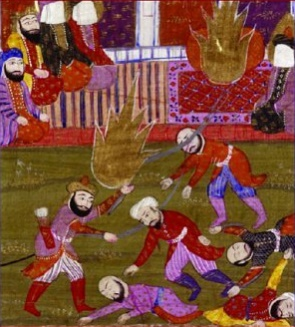
\includegraphics[width=1.31707in,height=1.45946in]{Images/image031.jpg}
    \caption{miniature du
19\textsuperscript{ème} siècle où l'on voit `Alī et Muḥammad massacrer
les membres de la tribu des Banū Qurayẓa. Manuscrit (17 folio 108b),
British Library.}
   
\end{marginfigure}
 
 



\paragraph{Le christianisme en
Arabie}

Un des archéologues, spécialiste du christianisme de la péninsule arabe,
est Christian Robin. {Le 18.08.2013, Sébastien de Courtois, dans l'émission
«~foi et tradition~» de France Culture, l'interroge. Il lui demande~tout
de go~: «~Alors Monsieur Robin, il y a eu une présence chrétienne en
Arabie
saoudite~?~»} 

Le Yémen a donc été «~officiellement~» chrétien entre 530 et 570. Son
roi est Abraha et, comme le dit Robin, on a découvert une inscription
qui date de 552 où sont mentionnées les régions soumises à son pouvoir~:
Arabie orientale, Arabie du Nord, Arabie du Nord-Est~; il y est aussi
question de Yathrib. Abraha a fait construire une cathédrale à San`ā'
{[}on est ici dans le sud de l'Arabie, l'Arabie heureuse{]} qui devient
capitale du Yémen, en 550. \emph{Les Chroniques} en donnent une
description détaillée, sublime. La cathédrale sera détruite au
8\textsuperscript{e} siècle.

Parmi les inscriptions, on dispose aussi d'une invocation à la Trinité
(\emph{Rahmanan}, son Fils \emph{Christos}, et l'Esprit Saint). Ce roi a
donc christianisé le Yémen et on ne trouve plus sous son règne
d'inscriptions spécifiquement juives.

\begin{marginfigure}
    \centering
    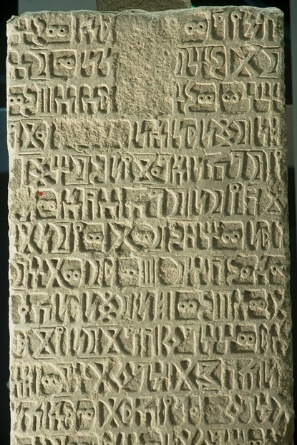
\includegraphics[width=1.31747in,height=1.96757in]{Images/image033.jpg}
    \caption{Inscription d'Abraha, 
    roi Éthiopien du Yémen, commémorant une réparation de la Digue de Marib }

\end{marginfigure}


le roi
Éthiopien du Yémen lors de la commémoration de la réparation de la Digue
de Marib et la consécration d'une église.~On y trouve aux premiers mots
l'invocation~
\begin{quote}
    « Avec la puissance, l'aide et la miséricorde de Rahmânân,
de son Messie et de l'Esprit Saint~» 
Christian Robin
\end{quote}

Mais la présence chrétienne dans le Yémen date déjà du
5\textsuperscript{e} siècle~: dans la \emph{Chronique de
Séert}\sn{Il s'agit d'une Chronique nestorienne d'auteur anonyme.
  Originellement écrite en syriaque, elle a été traduite en arabe.}, il
est question d'un commerçant de Najrān qui se serait converti lors d'un
séjour à al-Ḥīra en Irak.

Après quelques années, le chef de l'armée éthiopienne renverse le roi
installé et prend sa place. On a donc \textbf{un roi éthiopien sur le
trône du Yémen}, \textbf{en rupture avec l'Éthiopie}, qui affirme une
foi chrétienne, mais différente de son prédécesseur~: \textbf{son
lexique vient du syriaque et non de l'éthiopien}. Par ailleurs, il
supprime l'expression fils et parle de son messie. \textbf{Cela
ressemble à la christologie du Coran~: le Messie n'est plus appelé et
reconnu comme fils de Dieu.}

Dans le reste de la péninsule, il y a bien sûr une présence du
christianisme dans l'extrême nord-ouest. Byzance y joue un rôle
d'autorité. On trouve des communautés et des monastères sur la côte du
Golfe arabo-persique comme en témoignent des vestiges de ruines de
couvents découverts au Koweït, en Arabie saoudite et aux Émirats arabes
unis.

On trouve au Yémen une inscription monothéiste datant de 320~: c'est une
rupture avec les inscriptions païennes, mais également des inscriptions,
toujours du 4\textsuperscript{ème} siècle, utilisant un lexique nouveau,
emprunté au judéo-araméen. On y invoque un Dieu unique, souvent appelé
le Seigneur du ciel et de la terre. Probablement, le judaïsme a
influencé ces inscriptions.

\vide{luxe9sotuxe9risme-et-la-gnose-de-perse}{%
\paragraph{{1.2.4 L'ésotérisme et la gnose de Perse
}{1.2.4 L'ésotérisme et la gnose de Perse }}\label{luxe9sotuxe9risme-et-la-gnose-de-perse}}

Parmi les courants religieux présents en Arabie, il faut aussi faire
mention du mazdéisme et du manichéisme\sn{~Guy Monnot,
  \emph{Penseurs musulmans et religions iraniennes}, Études musulmanes
  n°16, Paris, Vrin, 1974.}. Tous deux ont joué un rôle non négligeable
dans la naissance de l'islam.

Le Coran évoque les mages (S. 22, 17), membres des castes mazdéennes.


\begin{quote}
{22. 17 }
{Certes, ceux qui croient, ceux qui pratiquent le judaïsme
ainsi que les sabéens, les chrétiens, les zoroastriens et les
polythéistes, Dieu les départagera le Jour de la Résurrection, car Il
est Témoin de toute
chose.}
{Inna allatheena amanoo waallatheena hadoo
waalssabieena waalnnasara waalmajoosa waallatheena ashrakoo inna Allaha
yafsilu baynahum yawma alqiyamati inna Allaha AAala kulli shayin
shaheedun
}
\end{quote}
\begin{marginfigure}
    \centering
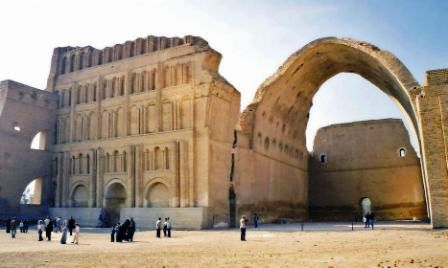
\includegraphics[width=\textwidth]{Images/image034.jpg}
    \caption{Tāq de Ctésiphon (Madā'in) en
Irak, à proximité duquel est enterré Salmān le
Perse}
    \label{fig:Ctesiphon}
\end{marginfigure}
Le mazdéisme est la religion officielle des Sassanides, dynastie perse
de 226 à 651. Mais on trouve des mazdéens en Irak, à Bahrayn, à Oman. Il
était pratiqué à La Mecque et Médine et au Yémen. Si les mazdéens
pratiquaient le rite du feu -- qui ne se retrouve pas en islam -- on
retrouve aussi dans leur religion \textbf{les cinq prières quotidiennes,
les rituels de prosternation, les rites d'ablution, la récitation de
textes sacrés, les sacrifices d'animaux}. Avant chaque geste important,
on prononçait la formule «~Au nom de Dieu~» qui trouve son pendant en
islam avec la \emph{basmala} que l'on récite avant les usages cultuels.
Au sein du mazdéisme, on trouve l'idée qu'il ne suffit pas de pratiquer,
mais que la pratique doit être motivée par l'intention. En islam, c'est
la \emph{niya} qui doit être formulée au début de chaque prière
quotidienne. \textbf{Sur le plan de la foi, le mazdéisme affirme
l'existence d'un créateur universel, d'une divinité dotée des attributs
de miséricorde, de justice, de bonté, il développe une vision
anthropologique où l'homme est d'abord parfait}~; du point de vue
eschatologique, il soutient la rétribution selon les actes posés et
l'épreuve de la pesée. Après la mort, l'âme reste auprès du mort avant
d'entreprendre un voyage. Là, elle passe sur le pont de Cinvad ~: pour
le juste, le pont s'élargit et conduit au paradis, mais pour le méchant,
il se rétrécit, devient fin comme une lame de rasoir, si bien qu'il
tombe dans les affres de l'enfer \textbf{Or, tous ces éléments se
retrouvent en islam}. Parmi les compagnons de Muḥammad, on compte un
mazdéen Salmān al-Fārisī (~m. 656), dit aussi Salmān le Perse, d'abord
converti au christianisme puis à l'islam et qui est considéré par Louis
Massignon, comme l'initiateur de l'islam iranien. Pour Louis Massignon
(nous avons déjà parlé de l'importance qu'il joua dans l'orientalisme du
vingtième siècle~et dit qu'il imposa l'usage du mot islam sur celui
d'islamisme, pour désigner la religion des musulmans), Salmān n'aurait
pas renié le Christ et serait donc un de ces personnages faisant la
jonction entre le christianisme et l'islam. Il a une grande importance
pour Massignon, car c'est près de sa tombe, un soir de mai 1908, que
celui-ci éprouva la «~Visitation de l'étranger~», qui comme un feu divin
est venu raviver les braises de sa foi\sn{Louis Massignon,
  «~Salmân ou les prémices spirituelles de l'Islam iranien~», in
  \emph{Parole donnée}, 1934.}.
\FloatBarrier



Pour ce qui est du \textbf{manichéisme}, il est apparu comme un courant
hétérodoxe du zoroastrisme, s'inspirant à la fois du bouddhisme, du
christianisme, du judaïsme, de la gnose, sur le fond du mazdéisme. C'est
une religion à vocation universelle, missionnaire donc, qui a pénétré la
péninsule arabique. Le père du premier calife omeyyade, Mu'āwiya, était
manichéen. Un certain nombre de particularités se retrouvent en islam.
Ainsi, par exemple, le \textbf{grand jeûne annuel des manichéens de
trente jours n'est pas sans rappeler le jeûne du Ramadan} -- durée
inconnue dans la Bible -- ou encore, l'interprétation de la tradition
musulmane selon laquelle Christ aurait été remplacé sur la croix par un
sosie (interprétation qui découle du commentaire du verset 4, 157~: les
juifs disent nous avons tué le Christ, mais ils ne l'ont ni tué, ni
crucifié, mais son sosie a été substitué à leurs yeux (\emph{šubbiha
la-hum}). Mais la ressemblance entre manichéisme et islam la plus
marquante concerne la prophétologie. \textbf{Le manichéisme est une
religion du Livre. Mani a reçu la visite de l'Ange de la prophétie et a
consigné dans un livre les révélations}. Contrairement à Zoroastre,
Jésus ou Bouddha, qui n'ont pas écrit eux-mêmes, la nouveauté consiste
en la rédaction personnelle du livre, évitant les falsifications opérées
par les disciples. Ce thème de la falsification des écritures se
retrouvera en islam. Notons aussi l'expression «~sceau des prophètes~».
Mani la fait sienne. Muḥammad sera ainsi appelé dans le Coran (S. 33,
40)
\begin{quote}
Muḥammad n'a jamais été le père d'un seul de vos hommes mais le messager
de Dieu, le \textbf{sceau des prophètes}, et Allāh est savant en toutes
choses.

\textbf{\TArabe{مَا كَانَ مُحَمَّدٌ أَبَا أَحَدٍ مِنْ رِجَالِكُمْ وَلَكِنْ
رَسُولَ اللَّهِ وَخَاتَمَ النَّبِيِّينَ وَكَانَ اللَّهُ بِكُلِّ شَيْءٍ
عَلِيمًا}}
\end{quote}


\section{Repères chronologiques et histoire des premiers
califes}

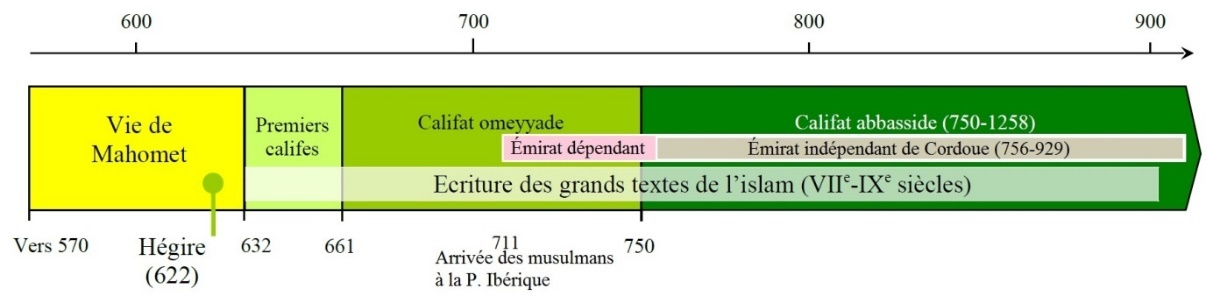
\includegraphics[width=\textwidth]{Images/image035.jpg}

Selon la tradition musulmane, Muḥammad est né vers 570. C'est en 610
qu'a lieu la première manifestation de la révélation du Coran -- nous y
reviendrons. 622 est l'année de l'hégire (\emph{hiǧra} en arabe)~: elle
renvoie au départ de Muḥammad de La Mecque pour Médine. Traduit parfois
par émigration, fuite (la vie de Muḥammad et des siens est menacée par
les Mecquois), la racine souligne l'idée de rupture des liens amicaux ou
familiaux.

\begin{Def}[muhāǧirūn et anṣār]
On appelle les Mecquois qui partirent avec Muḥammad
\textbf{les \emph{muhāǧirūn}, les émigrés.} Les Médinois qui se
convertirent à l'islam sont appelés \textbf{les \emph{anṣār}, les
auxiliaires}.
\end{Def}
La racine NaṢaRa signifiant venir en aide, apporter
protection.
Au moment du choix des premiers califes, grande sera la rivalité entre
les \emph{muhāǧirūn} et les \emph{anṣārs} où les appartenances tribales
ressurgissent.

La \emph{hiǧra} est au cœur du projet islamiste de Daesh qui a appelé
tous les musulmans à le rejoindre et à ainsi mettre ses pas dans ceux de
Muḥammad et de son émigration.

Les premiers califes sont désignés \emph{al-rāšidūn}, c'est-à-dire les
Bien-Guidés. C'est la période des quatre premiers califes~; dans l'ordre
chronologique~: Abū Bakr, ʿUmar, ʿUṯmān et ʿAlī.

\vide{abux16b-bakr-m.-634}{%
\subsubsection{{Abū Bakr (m. 634)
}{Abū Bakr (m. 634) }}\label{abux16b-bakr-m.-634}}

La tradition sunnite fait de lui le premier musulman après Ḫadiǧa,
l'épouse du jeune Muḥammad. Cette tradition permet aussi de légitimer le
rôle d'Abū Bakr et son institution comme calife, à l'issue de la mort de
Muḥammad, dans un contexte fébrile. D'ailleurs, sur la question de
savoir qui est le premier à avoir endossé l'islam, les šīʿites
considèrent quant à eux que c'est ʿAlī. À la mort de Muḥammad, une
élection eut lieu dans un contexte tendu où les opposants à Abū Bakr
furent absents et ne purent donc se prononcer. Par suite, un grand
mouvement se souleva pour s'opposer à ce choix. Certains refusèrent de
payer la zakāt. On appelle ce temps la période de la grande apostasie
(\emph{ridda}). Mais il faut bien voir qu'il s'agissait plus de
contester l'autorité d'Abū Bakr que de rejeter l'islam. Mais Abū Bakr et
ses partisans virent dans le non-paiement de la \emph{zakāt}, laquelle
est un pilier de l'islam, un acte d'apostasie. Il partit en guerre
contre les tribus récalcitrantes. La bataille d'al-Yamāma vit la mort de
plus de 1200 musulmans et 39 compagnons. Il meurt de maladie.

\vide{ux2bfumar-m.-644}{%
\subsubsection{ʿUmar (m. 644)}\label{ux2bfumar-m.-644}}

Il appartient à la tribu des Qurayš. Il a été nommé par Abū Bakr pour
lui succéder, après que ce dernier a consulté les compagnons. On le
surnomme \emph{al-Fārūq}, l'Équitable. Il fut l'un des premiers
opposants à l'islam et un défenseur des traditions mecquoises. Dans
certains récits sunnites, il est présenté comme ayant torturé des
musulmans pour qu'ils renient leur foi à l'exemple d'une servante des
Banū Mūʾammil. L'hégire dont nous avons parlé fut décidé par Muḥammad
dans le contexte de ces persécutions à La Mecque.

C'est à la suite de la conversation de sa sœur, Fāṭima, alors qu'il
était entré chez elle en colère et qu'il recourra à la violence contre
elle et son mari qu'on lui récita les versets de la Sourate ṬāHā
retranscrite sur un feuillet. À son récit, il se convertit. Il s'agit de
la Sourate 20. Voici les premiers versets

\mn{\emph{Au nom d'Allah, le Tout
Miséricordieux, le Très Miséricordieux.}\\
Pour entendre sa récitation en arabe avec le texte traduit en français~:
\url{https://www.youtube.com/watch?v=cXqHT-I5OgE}
}

\begin{quote}
    

1. Ṭā-Hā\\
{2.}
Nous n'avons point fait descendre sur toi le Coran pour que tu sois
malheureux,\\
{3.}
si ce n'est qu'un Rappel pour celui qui redoute (Allāh),\\
{4.}
(et comme) une révélation émanant de Celui qui a créé la terre et les
cieux sublimes.\\
{5.}
Le Tout Miséricordieux S'est établi \emph{«~Istawā~»} sur le Trône.\\
{6.}
À Lui appartient ce qui est dans les cieux, sur la terre, ce qui est
entre eux et ce qui est sous le sol humide.\\
{7.}
Et si tu élèves la voix, Il connaît certes les secrets, même les plus
cachés.\\
{8.}
Allah~! Point de divinité que Lui~! Il possède les noms les plus
beaux.\\
{9.}
Le récit de Moïse t'est-il parvenu~?\\
{10.}
Lorsqu'il vit du feu, il dit à sa famille~: «~Restez ici~! Je vois du
feu de loin; peut-être vous en apporterai-je un tison, ou trouverai-je
auprès du feu de quoi me
guider»\\
{11.}
Puis, lorsqu'il y arriva, il fut interpellé~: «~Moïse~!\\
{12.}
Je suis ton Seigneur. Enlève tes sandales~: car tu es dans la vallée
sacrée, Ṭuwā.\\
{13.}
Moi, Je t'ai choisi. Ecoute donc ce qui va être révélé.
\end{quote}
ʿUmar est aussi connu pour avoir convaincu Abū Bakr de la nécessité de
rassembler le Coran. Désigné comme son successeur par Abū Bakr peu de
temps avant sa mort, il est le premier à être appelé \emph{Amīr
al-mūmīnīn}, c'est-à-dire Commandeur des croyants ou Prince des
Croyants.


\mn{Aujourd'hui, ce titre est celui du roi du
Maroc~: Article 41 de la
{Constitution
de 2011} :
«~Le Roi, Amir al-Mouminine, veille au respect de l'Islam. Il est Garant
du libre exercice des cultes. Il préside le Conseil supérieur des
Oulémas, chargé de l'étude des questions qu'Il lui soumet~».
}

Ce titre est aussi celui qu'a revendiqué pour lui Abū Bakr al-Baġdādī de
l'État islamique. Remarquez son nom~: celui du premier calife de
l'islam.

C'est ʿUmar qui est à l'initiative du nouveau calendrier musulman.

Chef de guerre, c'est sous son califat que les Arabes se rassemblèrent
et prirent Damas avant de conquérir l'Irak et la Perse~; puis il envoya
Muʾāwiya à la conquête de Jérusalem. Dans une lettre adressée au
Patriarche Sophrone, il assura sa protection aux habitants de la ville
et la sauvegarde des lieux chrétiens.

Il se rendit à Jérusalem, alla prier sur l'Esplanade du Temple où selon
la Sourate 17\textsuperscript{ème}, Muḥammad s'était rendu en songe
durant une nuit. C'est alors que sera construite le Dôme du Rocher,
\emph{Qubbat al-ṣaḫra} par le calife ʿAbd al-Malik. Ce Dôme est souvent
appelé Mosquée de ʿUmar, mais à tort. \\


Il meurt poignardé par un esclave zoroastrien. Concernant sa succession,
il a pris soin de nommer un conseil électoral de six électeurs, une
\emph{šūra}, qui doit élire son successeur. Ce conseil, composé
principalement des \emph{mūhaǧirīn}, visait à écarter du pouvoir les
\emph{anṣār}. Ce conseil sert aujourd'hui à certains penseurs musulmans
pour penser la démocratie du point de vue islamique.

 
\subsubsection{ʿUṯmān (m. 656)
} 
C'est selon la tradition musulmane un des premiers compagnons de
Muḥammad~; sa conversion est antérieure à l'Hégire. En 620, lors du
départ d'un groupe de musulmans pour l'Abyssinie, ʿUṯmān faisait partie
des émigrants. Il a épousé deux filles de Muḥammad. Il poursuit une
politique de conquête qui l'amène jusqu'en Arménie, en Égypte, en Nubie,
au Maghreb.

On lui doit d'avoir mené à bien la recension officielle du Coran. Nous
en reparlerons.

Il est assassiné à Médine en 656.

\vide{ux2bfalux12b-m.-661}{%
\subsubsection{ʿAlī (m. 661)}\label{ux2bfalux12b-m.-661}}

Il est nommé calife~et renvoie un certain nombre de gouverneurs qui
avaient été nommés par ʿUṯmān. La capitale est transférée à Kūfa. Son
califat est marqué par de profondes divisions~: c'est la première
\emph{\textbf{fitna}}, ou guerre de sédition.

Sur le plan théologique, il laisse des sermons et une œuvre monumentale
au titre évocateur intitulée \emph{Le sommet de l'éloquence},
\emph{Nahǧul Balaġa}. Il est possible de lire ces sermons
\sn{\url{http://www.orient-lib.com/A-52389-nahj-al-balagha-la-voie-de-l-eloquence-arabe-francais.aspx}{en
français}}. Après le Coran et la Sunna, l'ouvrage est le plus étudié dans
le šīʿisme. On y trouve une théologie de la création du ciel, de la
terre et des anges, mais aussi une personnification du Jour du Jugement
dernier. Écrit aussi sous forme d'adages ou de proverbes, l'ouvrage
nourrit des générations de musulmans sur le plan de la morale des
vertus.

Écarté dans un premier temps par Abū Bakr, ʿAlī avait refusé de mener le
combat car il a toujours privilégié l'entente entre les musulmans. S'il
est un personnage central dans le šīʿisme, ʿAlī est aussi une des
références sunnites~comme quatrième calife~: on ne sera donc pas surpris
de trouver dans les sources sunnites des paroles laudatrices à son
égard. C'est le cas notamment des \emph{ḥadīṯs} suivants :

Suyūtī (m. 911/1505) {[}c'est un grand savant égyptien expert en
\emph{ḥadīṯ}. Son nom reviendra par la suite{]} rapporte d'Ibn Abbas le
\emph{ḥadīṯ} suivant~:

«~\textbf{Je suis la Cité du Savoir. ʿAlī en est sa Porte; quiconque
recherche le Savoir, doit franchir le seuil de cette Porte.}~»

Autre \emph{ḥadīṯ}~rapporté par al-Ṭabarānī~(m. 360/970) : {[}À son
époque, il passait pour être le plus expert en science du ḥadīṯ{]}
\begin{quote}
«~{Il y a cette inscription sur la Porte du Paradis: Il n'y a de
Allah que Allah ; Muḥammad est le Messager de Allah ; et ʿAlī est le
frère du Messager}~».~
\end{quote}


~Ce \emph{ḥadīṯ} est intéressant car il on y trouve des éléments de la
profession de foi (premier pilier de l'islam) des šīʿites~duodécimains :
«~et ʿAlī est le walī d'Allāh~».

Sur le plan militaire, il doit affronter le gouverneur de Damas,
al-Mu'āwiya. Lors de la bataille de Siffin contre ce gouverneur, il
accepte un arbitrage qui est finalement en sa défaveur. Il se retire
alors à Koufa mais nombreux sont ceux qui lui reprochent d'avoir accepté
cet arbitrage alors que Dieu lui assurait la victoire. Certains de ses
partisans décidèrent de le quitter, ce sont les \emph{ḫariǧites} (de la
racine ḪaRaǦa~: sortir). Il est assassiné par l'un d'eux.

\begin{marginfigure}
    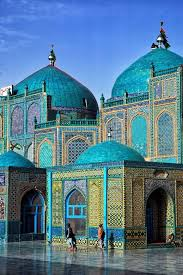
\includegraphics[width=1.06615in,height=1.6045in]{Images/image037.jpg}
    \caption{La mosquée bleue en Afghanistan est supposée être le lieu
du tombeau de ʿAlī. Rawze-i-Sharif (La Mosquée du Saint en référence à
Hazrat-e Ali Ibn Talib}
\end{marginfigure}


Par la suite, l'islam se structure autour de deux empires successifs,
rivaux~: l'empire omeyyade puis l'empire abbasside. Mais revenons à la
péninsule arabe à la naissance de l'islam et à son univers religieux.

\textbf{Conclusion}

Au départ de notre réflexion, une question~: comment connaître le
contexte culturel, religieux, politique de l'Arabie antéislamique~? Nous
remarquions que si nous disposons de sources musulmanes, elles ne
sauraient suffire, d'autant qu'elles participent d'une reconstruction
historique mettant en lumière le monde chaotique dans lequel se
trouvaient les tribus arabes avant la prédication de Muḥammad.

Cette difficulté épistémologique se retrouve dans l'histoire de l'islam
naissant et des premières dynasties. Or, il n'est pas possible de faire
l'histoire des premiers siècles sur la base des seules sources
musulmanes. Julius Wellhausen et Henri Lammens ont montré les failles de
l'histoire telle que la raconte l'historien al-Ṭabarī~: (nous l'avons
rencontré dans le commentaire de la bibliographie\ldots{} son traducteur
et analyste est Claude Gilliot). Je voudrais donner un exemple de ces
prismes au moment de la chute des Omeyyades en 750\sn{Sabatino
  Moscati, «~Le massacre des Umayyades dans l'histoire et dans les
  fragments poétiques~», Archiv Orientalni 18, 1950, p. 88-115.}.
L'histoire des Omeyyades, première dynastie de l'islam, est en effet
connue à partir de textes rédigés après l'arrivée des Abbassides. Or, si
le berceau des Omeyyades est la Syrie, les historiens écrivent dans
l'Irak abbasside à la fin du 9\textsuperscript{e} siècle après la
réinstallation du califat à Bagdad. Antoine Borrut montre qu'il fallait
réécrire l'histoire car «~les signes de continuité étaient devenus
inintelligibles~» après 150 ans de domination abbasside~:

«~Les épisodes successifs de la Révolution abbasside, de la guerre
civile entre les fils d'al-Rašīd, de la miḥna, du déplacement du califat
à Sāmarrā', de l'essor des militaires turcs, de l'assassinat
d'al-Mutawakkil et de la perte de la réalité du pouvoir par le calife,
suffisent amplement à expliquer cette perte de repères et le déficit de
cohérence dont souffrait alors l'histoire islamique~»\sn{Cité par
  Françoise Micheau, \emph{Les débuts de l'islam}, Paris, 2012, p. 28.}.

Il fallait donc rattacher directement les Abbassides à l'origine de
l'islam et faire tomber dans l'oubli la période omeyyade. Le massacre
des Omeyyades en 750 par les Abbassides est totalement omis dans
certains textes historiques. Al-Ṭabarī est pudique dans sa description
-- il faut dire qu'il fait désordre et pour fonder la légitimité
politique\ldots{} on peut faire mieux. Ibn Qutayba (m. 276/889) et
al-Mas`ūdī (m. 345/956) sont aussi peu prolixes. Les noms de ces trois
grands historiens ont déjà été mentionnés. Je redonne ici les dates avec
le calendrier hégirien\ldots{} alors que la première fois, je n'avais
mis que le calendrier grégorien\sn{Le calendrier hégirien est le
  calendrier musulman. L'année 0 est l'année de l'hégire, c'est-à-dire
  de la fuite de Muḥammad lorsqu'il quitte La Mecque. Nous sommes en 622
  dans le calendrier grégorien.}.

\textbf{La destruction des tombeaux des califes par les abbassides est
symptomatique de cette volonté de l'oubli. Mais malgré tout, les lieux
sont là et sont aujourd'hui redécouverts. Ils donnent de nouvelles
lumières sur les fondations de l'islam et l'histoire des premiers
siècles.} %2
\FloatBarrier
\chapter{Les biographies de Muḥammad, Prophète de l'islam}

Après avoir abordé le milieu religieux de la péninsule arabique à l'aube
du VIIe siècle, et distingué à grands traits les grandes dates de la
naissance de l'islam, il convient à présent de focaliser notre attention
sur celui qui est considéré par les musulmans comme le messager de la
Révélation coranique, Mahomet ou Muḥammad (مُحَمَّد). Personnellement,
j'écris Muḥammad qui est la translittération du nom du Prophète de
l'arabe en français, tandis que Mahomet est l'écriture francisée, venant
du latin Mahometus. Que sait-on de lui~? Comment vivait-il~? À quelle
religion appartenait-il~? A-t-il fréquenté des juifs, des chrétiens et
des mazdéens de La Mecque~? Comment sa prédication a-t-elle été reçue~?
Quand parvient-il à imposer la légitimité de sa mission~? Comment s'y
prend-il~? Quelles relations entretient-il avec son clan~? Sa tribu~?
Était-il prophète, roi et chef de guerre, comme on le dit~?

Les questions sont posées. Elles sont importantes. J'en pose une autre,
au préalable~: Comment fait-on pour savoir~? Comment s'y prend-on pour
répondre~? En historien, on s'appuie forcément sur des sources, en
portant sur elles un regard critique, et ce d'autant plus que la
première «~biographie~» de Muḥammad date de la fin du VIIIe
siècle\ldots{} donc du temps des abbasides. Le temps a passé, il y a
déjà eu l'ère des califes bien guidés, les Rashidūn (cela a donné le
prénom Rashid, au féminin~: Rashida), puis celui de l'empire des
Omeyyades. Si vous ne voyez pas qui sont les califes bien guidés,
relisez le chapitre 2. Or, écrire une biographie n'est jamais neutre.

Certes, une lecture croyante peut fort bien vouloir se dispenser des
études critiques sur les fondations de l'islam, mais comme l'écrit
l'historien tunisien Hichem Djaït dans la biographie qu'il consacre à
Muḥammad~: «~la science est une, et le souci de scientificité est la
marque des sociétés libres~»\sn{Hichem Djaït, La vie de Muḥammad,
  Volume 2, Paris, Fayard, 2008 p. 13.}.

Il me semble donc incontournable de consacrer quelques pages du cours à
la question épistémologique : de quelles sources disposons-nous~? Quel
est leur statut~?

Mais la question des sources posées, il faut constater que la figure
même de Muḥammad a donné lieu à de multiples biographies au cours des
siècles. C'est le pluriel qui s'impose. Certes, il y a les premières
grandes biographies dont la matrice est donnée par Ibn Iṣḥāq (ابن
إسحاق), mais au cours des siècles va se développer des images de
Muḥammad et cela jusqu'à nos jours. Quelles sont ces images~?

Dans ce chapitre sur les fondations de l'islam, il nous semble opportun
de donner aussi quelques passages de ces premières biographies. À cet
égard, je m'appuierai sur les textes de la Sīra d'Ibn Hishām, car c'est
la plus populaire. Le préambule méthodologique permettra aussi
d'analyser ces informations~dans les contextes politiques et religieux
où elles ont été données.

\vide{la-question-muxe9thodologique-comment-uxe9crire-la-biographie-de-muux1e25ammad}{%
\subsubsection{{La question méthodologique~: comment écrire la biographie de Muḥammad~? }}\label{la-question-muxe9thodologique-comment-uxe9crire-la-biographie-de-muux1e25ammad}}

En arabe, la biographie de Muḥammad s'appelle Sīra. Aujourd'hui, les
biographies du Messager de l'islam ne manquent pas. En français, il y a
celles écrites par des musulmans à l'exemple d'Al-Sira de Mahmoud
Hussein -- pseudonyme commun de Bahgat Elnadi et Adel Rifaat,
politologues français d'origine égyptienne --, de Tariq Ramadan,
Muhammad, La vie du Prophète ou encore de l'historien tunisien Hichem
Djaït, La vie de Muḥammad, écrite en trois volumes parus en français aux
éditions Fayard et que nous avons déjà cité ci-dessus.

On trouve aussi celles des orientalistes comme Maxime
Rodinson\sn{Maxime Rodinson, Mahomet, Paris, 1956.}, Tor
Andrae\sn{Tor Andrae, Les Origines de l'islam et le christianisme,
  tr. fr., Paris, 1955.}\textsuperscript{,} Régis Blachère, W.
Montgommery Watt\sn{Montgomery Watt, Mahomet à La Mecque~; Mahomet
  à Médine, trad. Fr., Paris, 1958 et 1959.}, Jacqueline Chabbi et son
livre \emph{Le Seigneur des tribus}. La dernière en date de ce point de
vue est celle écrite par l'orientaliste allemand Tilman Nagel. Les
approches entre les biographies confessantes et les biographies
historiques sont bien sûr différentes, très différentes. Mais il faut
bien voir que pour les musulmans, la biographie n'est pas une écriture
a-historique. Au contraire, la biographie du Prophète est
intrinsèquement liée à celle de l'histoire de la naissance de l'umma. Il
s'agit d'approcher Muḥammad, son univers culturel, mais aussi social.
Les historiens musulmans ont le souci de rendre compte des moindres
personnages ayant fréquenté Muḥammad, mais aussi de ses gestes
quotidiens. Tarif Khalidi dans \emph{Images of Muḥammad} dit qu'avec la
Sīra, c'est un peu comme si on avait voulu retranscrire le nom des 5 000
personnes venues écouter le Sermon sur la montagne de Jésus. Ce genre de
biographies de la première communauté s'appelle les \emph{Tabaqāt}.
C'est un genre littéraire typique de l'islam. Par ailleurs, si dans les
Évangiles, on sait peu de choses de la vie privée de Jésus, la Sīra
aborde aussi bien la vie publique que la vie privée et intime de
Muḥammad\sn{Tarif Khalidi, Images of Muḥammad. Narratives of the
  Prophet in Islam. Across the Centuries, New York, Doubleday, 2009.}.

Dans un article paru dans la revue \emph{History Compass} en 2007,
Robert Hoyland présente les différents points de vue et méthodologies
mises en œuvre en vue de dessiner un portrait authentique de
Muḥammad\sn{Robert Hoyland, «~Writing the Biography of the Prophet
  Muḥammad~: Problems and Solutions~», History Compass, 5/2, 2007, p.
  581-602.}. Dans tous les cas, l'intention est la même~: se rapprocher
de la réalité.

Hoyland souligne dans un premier temps que l'image du Prophète Muḥammad
qui est véhiculé du côté occidental a d'abord été négative~: Muḥammad
(ou ceux qui se revendiquent de son message) conquiert des terres et
impose une religion en portant un message qui au final nie la divinité
du Christ. On va y voir un homme d'ambition et de passion, au pire la
figure de l'Antéchrist, le fils du diable. L'époque médiévale applique
la parole de Jésus sur les faux prophètes. Dans la \emph{Somme contre
les Gentils} Saint Thomas d'Aquin avance les preuves rationnelles de
l'impossibilité pour Muhammad d'être dit «~prophète~»\sn{«~Par
  contre, il {[}Mahomet{]} a entremêlé les vérités de son enseignement
  de beaucoup de fables et de doctrines les plus fausses. Il n'a pas
  apporté de preuves surnaturelles, les seules à témoigner comme il
  convient en faveur de l'inspiration divine, à savoir quand une œuvre
  visible qui ne peut être que l'œuvre de Dieu prouve que le docteur de
  vérité est invisiblement inspiré. Il a prétendu au contraire qu'il
  était envoyé dans la puissance des armes, preuves qui ne font point
  défaut aux brigands et aux tyrans. ~Aucune prophétie divine ne
  témoigne en sa faveur : bien au contraire, il déforme les
  enseignements de l'Ancien et du Nouveau Testament par des récits
  légendaires, comme c'est évident pour qui étudie sa loi. Aussi bien,
  par une mesure pleine d'astuces, il interdit à ses disciples de lire
  les textes de l'Ancien et du Nouveau Testament qui pourraient le
  convaincre de fausseté.~»}. Au xvième, Luther dans un essai de 1528,
\emph{De la guerre contre les Turcs} (Vom Kriege wider die Türken)
expose l'incompatibilité de l'islam avec la foi chrétienne. Dans le
contexte de l'invasion ottomane en Europe et du Siège de Vienne, il
appelle à la résistance contre les turcs et, si Muḥammad ne peut
l'Antéchrist, puisque c'est le pape qui l'est, il ne peut donc être
qu'un «~démon~», le fruit du mensonge, celui qui fait table rase de la
vérité chrétienne, qui détruit «~l'ordre spirituel de la foi et de la
vérité~»\sn{Pour une étude sur Muḥammad et l'islam chez Luthern
  voir~: A.S Francisco, Martin Luther and Islam. A Study in
  Sixteenth-Century Polemics and Apologetics, coll. The History of
  Christian-Muslim Relations 8, Leiden, Brill, 2007.}. Cette vision est
encore celle du philosophe Pascal au xviie siècle.

Les lumières apportent un regard renouvelé sur l'islam qu'il s'agit
d'intégrer à une vision universelle de l'humanité, et au XIXème siècle,
d'une manière surprenante, Ernest Renan dans \emph{Mahomet et les
origines de l'islamisme}, écrit~:

«~La vie de son fondateur nous est aussi bien connue que celle de tel
réformateur du xvie siècle. Nous pouvons suivre année par année les
fluctuations de sa pensée, ses contradictions, ses faiblesses~».

Cet optimisme repose sur l'assurance en l'authenticité des paroles et
gestes consignés par la tradition musulmane. Or, au \textsc{XIXème}
siècle, l'orientaliste Ignaz Goldziher est le premier à avoir, mis en
avant l'aspect reconstruit du \emph{ḥadīṯ} et il concluait qu'il ne peut
constituer un matériel historique pour rendre compte de la naissance de
l'islam~; il permet cependant de mettre en lumière des tendances
dogmatiques ou juridiques qui se sont développées au cours des premiers
siècles. Henri Lammens au début du XXème siècle publie en 1912
\emph{Fatima et les filles de Mahomet}: \emph{notes critiques pour
l'étude de la Sira}. Il montre que

«~l'inspiration de la Sīra est d'abord exégétique. Dérivée en droiture
du texte du Qoran, la Sīra est destinée à lui servir de commentaire en
action~; elle doit traduire, en anecdotes précises et pittoresques, les
allusions les plus obscures, les sous-entendus les moins intelligibles
des versets, faire la chasse à l'anonyme, à l'impersonnel, si
déconcertants dans la lecture des sourates, partout, pour ainsi dire,
apposer des plaques commémoratives, multiplier la mention des noms
propres, les dates, si prudemment évités par Abou'l Qasim~»\sn{Henri
  Lammens, Fatima et les filles de Mahomet: notes critiques pour l'étude
  de la Sīra, Rome, Institut Biblique Pontifical, 1912, p. vii.}.

Bref, la Sīra doit combler l'obscurité du Coran, elle doit l'expliquer,
l'historiciser, mais elle vise aussi à préciser la doctrine coranique et
la jurisprudence. Ainsi, il existait parmi les juristes de Médine et
ceux de La Mecque et d'Irak, deux positions relatives à la possibilité
pour un pèlerin de contracter un mariage. De part et d'autre, la vie de
Muḥammad et ses paroles vont être convoquées pour fonder leur position,
quitte à ce qu'il y ait contradiction. Joseph Schacht conclut que bien
des éléments de la vie de Muḥammad, des détails importants, ne sont pas
fondés sur une recollection authentique mais sont fictifs et servent à
défendre des doctrines juridiques. L'articulation entre la vie du
Prophète et l'exégèse n'a pas perdu de son actualité~: c'est la
perspective de Patricia Crone~: «~Une grande partie de la tradition
apparemment historique est en fait d'origine exégétique~»\sn{Patricia
  Crone, Meccan Trade and the Rise of Islam, Oxford, 1987, p. 214.}.

De ces difficultés, certains orientalistes ont cherché à approcher
Muḥammad à partir du Coran seul. C'est le cas de Régis Blachère. Mais
cette approche est aussi celle de musulmans qu'on appelle les
\textbf{coranistes}~: pour eux, l'islam c'est le Coran et seulement le
Coran. Cependant, ce n'est pas sans difficulté car le Coran est peu
prolixe sur son environnement et à l'exception des noms bibliques, on ne
trouve que deux noms de personnages qui sont mentionnés~: celui de
Muḥammad, à quatre reprises, et celui d'Abū Lahab.

\vide{uxe0-propos-dabux16b-lahab-que-lon-trouve-dans-la-sourate-111-1-5}{%
\subsubsection{{À propos d'Abū Lahab que l'on trouve dans la sourate 111, 1-5~: }}\label{uxe0-propos-dabux16b-lahab-que-lon-trouve-dans-la-sourate-111-1-5}}

\begin{quote}
    Que périssent les deux mains d'Abū Lahab
et que lui-même périsse. Sa fortune ne lui sert à rien, ni ce qu'il a
acquis. Il sera brûlé dans un feu plein de flammes, de même sa femme, la
porteuse de bois, à son cou une corde de fibres.
\end{quote}


On apprend par les commentaires qu'il
s'agit de son oncle, hostile à Muḥammad et que la femme est surnommée la
porteuse de bois car elle jetait du bois et des plantes épineuses sur la
route qu'empruntait le Prophète\ldots{} mais sans les commentaires, le
Coran lui-même reste très énigmatique.


Le Coran fait aussi mention des Romains et de la tribu de Quraysh, mais
pas des autres tribus. Huit lieux sont indiqués, quatre communautés
religieuses (juifs, chrétiens, mages et sabéens) ainsi que trois
divinités arabes. Et si La Mecque est nommée, aucune indication sur son
rôle dans la vie de Muḥammad. Il est question dans le Coran de Badr mais
rien ne permet d'y voir une référence explicite à la fameuse bataille du
même nom, même si l'interprétation est possible.

\vide{uxe0-propos-de-la-bataille-de-badr}{%
\paragraph{À propos de la bataille de
Badr}\label{uxe0-propos-de-la-bataille-de-badr}}

C'est la première grande bataille militaire que mène Muḥammad après son
exil à Médine contre une caravane de Mecquois. Une armée d'hommes
accompagnée de milliers d'anges vont emporter leur première victoire
contre les notables de La Mecque~; Muhammad y acquiert le prestige de
fin stratège.

Selon les commentaires coraniques, le Coran ferait allusion à cette
bataille~:




\begin{table}[h!]
\resizebox{\textwidth}{!}{%
\small
\begin{tabular}{p{7cm}p{7cm}}

Il y eut déjà pour vous un signe dans ces deux troupes qui
s'affrontèrent: l'une combattait dans le sentier d'Allah; et l'autre,
était mécréante. Ces derniers voyaient les croyants de leurs propres
yeux, deux fois plus nombreux qu'eux-mêmes. Or Allah secourt qui Il veut
de Son aide. Voilà bien là un exemple pour les doués de clairvoyance !
& 

\\

S. 3, 123~ Allah vous a donné la victoire, à Badr, alors que vous étiez humiliés.
Craignez Allah donc. Afin que vous soyez reconnaissants! &  
\TArabe{

وَلَقَدْ نَصَرَكُمُ اللَّهُ بِبَدْرٍ وَأَنتُمْ أَذِلَّةٌ فَاتَّقُوا
اللَّهَ لَعَل

َّكُمْ تَشْكُرُونَ }
\\

\end{tabular}%
}
\sidecaption{La bataille de Badr S. 3, 13 et 123}
\end{table}



 

\vide{badr}{%
{{\includegraphics[width=1.27898in,height=2.02315in]{Images/image38.jpeg}}{Badr}}\label{badr}}

\vide{la-bataille-de-badr}{%
\subsubsection{La bataille de Badr}\label{la-bataille-de-badr}}

\vide{section-7}{%
\subsubsection{}\label{section-7}}

\vide{remarquez-lange-gabriel-qui-annonce-la-victoire-uxe0-muux1e25ammad.-le-visage-du-prophuxe8te-est-voiluxe9.}{%
\mn{{Remarquez l'ange Gabriel qui annonce la
victoire à Muḥammad. Le visage du Prophète est voilé.
}{Remarquez l'ange Gabriel qui annonce la victoire à Muḥammad. Le visage du Prophète est voilé. }}\label{remarquez-lange-gabriel-qui-annonce-la-victoire-uxe0-muux1e25ammad.-le-visage-du-prophuxe8te-est-voiluxe9.}}

\vide{au-milieu-entre-les-combattants-de-leau-badr-est-le-nom-dun-puits-deau.-pour-muux1e25ammad-il-est-en-cela-un-lieu-stratuxe9gique-dans-la-mesure-ouxf9-la-caravane-devra-sy-arruxeater.}{%
\paragraph{Au milieu, entre les combattants, de l'eau : Badr est le
nom d'un puits d'eau.} Pour Muḥammad il est en cela un lieu stratégique
dans la mesure où la caravane devra s'y
arrêter.}\label{au-milieu-entre-les-combattants-de-leau-badr-est-le-nom-dun-puits-deau.-pour-muux1e25ammad-il-est-en-cela-un-lieu-stratuxe9gique-dans-la-mesure-ouxf9-la-caravane-devra-sy-arruxeater.}

Dans\textit{ De la guerre}, Carl von Clausewitz a dressé la théorie de
l'importance du puits d'eau dans le combat.

Dans ce contexte, Montgomerry Watt a réhabilité le matériel traditionnel
dans sa biographie de Muḥammad notamment tout ce qui a trait aux
expéditions militaires dans la mesure rien ne ces textes ne cherchent à
expliciter le Coran, le commenter, et que de la même manière il ne
s'agit pas de développements doctrinaux ou jurisprudentiels.

De ces avertissements, de ces difficultés, il s'ensuit que le biographe
de Muḥammad est pris entre deux tenailles~: à la fois il encourt le
risque de rejeter tout matériel historique comme étant une pieuse
invention ou d'intégrer à la réalité historique des éléments de légende
et des inventions. Et finalement, comme le dit Maxime Rodinson, on
risque d'écrire une biographie en fonction de ses propres intérêts,
questions, présupposés, intuitions, comme à l'époque de la tradition
musulmane.

Fort de ces difficultés, à laquelle s'ajoute une idéalisation de la
figure de Muḥammad comme guide à suivre et modèle à imiter, Tilman Nagel
a cherché à «~déchiffrer les conceptions religieuses~» de Muḥammad en
remontant au-delà des sources normatives. Il a utilisé des données de la
poésie, les sources extra-islamiques, l'histoire préislamique de La
Mecque et Médine. Il en arrive au schéma chronologique suivant~:

\begin{itemize}
\item
  Muḥammad annonce le Dieu Unique aux Mecquois. Dans le Coran, il est
  dit \textbf{avertisseur}.
\item
  Vers 620, il élargit son message et se considère désormais comme
  Prophète de Dieu (Allāh). C'est à partir de cette date que l'on voit
  apparaître les notions de nabī et rasūl (prophète). Il n'appelle pas
  seulement à adorer Dieu, mais désormais il expose le rite religieux et
  les règles de vie voulues par Allāh.
\item
  Rejeté par les habitants de La Mecque qui refusèrent ses commandements
  sur le culte, il part pour Médine où son clan a des relations avec
  l'une des tribus médinoises.
\item
  À Médine, il ne peut plus participer au pèlerinage annuel de La
  Mecque. Comme prophète, il doit aussi s'imposer comme chef. Il mena
  donc des opérations militaires contre sa ville natale de 624 à 627.
\item
  Il finit par s'imposer sur les mecquois. Il devient la référence
  politique et religieuse, mais aussi morale, d'où la dimension de plus
  en plus normative. Il s'est ainsi imposé comme l'unique autorité de ce
  qui est juste et équitable, mais aussi le modèle spirituel et moral.
\end{itemize}

Et Tilman Nagel de conclure à l'existence de deux Muḥammad~: le
\textbf{Muḥammad historique}, prédicateur, militaire et le
\textbf{Muḥammad idéalisé}. La tradition a très vite superposé les deux
images de Muḥammad et a historisé le Muḥammad idéalisé si bien que toute
critique à l'égard de Muḥammad entouré d'un halo de sainteté est perçue
comme un acte blasphématoire, un sacrilège et explique que dans certains
pays, blasphémer contre le prophète est considéré comme un acte
criminel.

Mais venons-en à présent à ces sources musulmanes et voyons comment
Muḥammad est présenté au cours du temps, voyons quelles sont ses vies.


\section{Les sources arabes de la biographie de
Muḥammad}
\label{les-sources-arabes-de-la-biographie-de-muux1e25ammad}


\subsection{Muḥammad dans le
Coran}
\label{muux1e25ammad-dans-le-coran}

C'est bien sûr dans le Coran que l'on trouve les premières mentions de
Muḥammad. Mais si les références aux prophètes de la Bible sont
nombreuses, Muḥammad n'y est cité que quatre fois. Comme avec les autres
prophètes, le Coran est peu bavard. Il est tour à tour un avertisseur
(naḏīr), puis un prophète (nabī), un messager (rasūl) qui vient apporté
la Parole. Par rapport aux autres prophètes, Muḥammad a un titre
spécifique~: «~\emph{il est le sceau des prophètes}~» (S. 33, 40).

\begin{longtable}
{p{6cm}p{6cm}}
\toprule

«~Muhammad n'a jamais été le père de l'un de vos hommes, mais le
messager d'Allah et le sceau des prophètes. Allah est Omniscient~». & 
\TArabe{
مَّا كَانَ مُحَمَّدٌ أَبَا أَحَدٍ مِّن رِّجَالِكُمْ وَلَكِن رَّسُولَ
اللَّهِ وَخَاتَمَ النَّبِيِّينَ وَكَانَ اللَّهُ بِكُلِّ شَيْءٍ
عَلِيمًا 
}\\
\bottomrule
\end{longtable}

Comme pour les autres prophètes, Muḥammad n'est pas écouté et il est
même l'objet de la risée de sa communauté. En ce sens, il suit un topos
prophétique dont le Coran se fait lui-même l'écho~:

\begin{longtable}{p{6cm}p{6cm}}
\toprule
\endhead
«~Hélas pour les esclaves {[}les humains{]}! Jamais il ne leur vient de
messager sans qu'ils ne le raillent~». &\TArabe{ يَا حَسْرَةً عَلَى الْعِبَادِ
مَا يَأْتِيهِم مِّن رَّسُولٍ إِلَّا كَانُوا بِهِ يَسْتَهْزِئُونَ }\\
\bottomrule
\end{longtable}

Le Coran fait mention explicite des accusations dont il est l'objet~au
sein de sa communauté : il est accusé d'être un sorcier (sāḥir,
سَاحِرٌ), ensorcellé (masḥūr, مَّسْحُورٌ) d'être possédé par un djīn
(maǧnūn, مَجْنُونٌ), d'être un devin (kāhin) d'être enseigné par
quelqu'un (muʿallamun, مُعَلَّمٌ), d'être un poète (šāʿir), d'être un
raconteur de fables. Mais là encore, il s'agit d'inscrire ces
accusations dans une filiation si bien que par ce procédé rhétorique,
elles deviennent la preuve de sa véracité~:

\begin{longtable}{p{6cm}p{6cm}}
\toprule
\endhead
«~Ainsi, aucun Messager n'est venu à leurs prédécesseurs sans qu'ils
n'aient dit: «C'est un magicien ou un possédé!~» (S. 51, 52) &\TArabe{ كَذَلِكَ
مَا أَتَى الَّذِينَ مِن قَبْلِهِم مِّن رَّسُولٍ إِلَّا قَالُوا سَاحِرٌ
أَوْ مَجْنُونٌ }\\
\bottomrule
\end{longtable}

Sur la poésie, il y aurait beaucoup à dire. Le Coran n'est pas favorable
aux poètes~: pour lui, ils divaguent et s'égarent (S. 26, 224-226), et
l'enseignement donné à Muḥammad ne relève pas de la poésie (S. 36, 69).

Quant à l'accusation d'être un raconteur de légende, on en trouve une
expression virulente dans S. 25, 5)~:

\begin{longtable}{p{6cm}p{6cm}}
\toprule
\endhead
«~Et ils {[}les mécréants{]} disent: `Ce sont des contes d'anciens qu'il
se fait écrire! On les lui dicte matin et soir!'~» &\TArabe{ وَقَالُوا
أَسَاطِيرُ الْأَوَّلِينَ اكْتَتَبَهَا فَهِيَ تُمْلَى عَلَيْهِ بُكْرَةً
وَأَصِيلًا }\\
\bottomrule
\end{longtable}

Face à ces accusations, le Coran prend sa défense, mais il se fait aussi
menaçant (S.9, 61)

\begin{longtable}{p{6cm}p{6cm}}
\toprule
\endhead
«~Ceux qui font du tort au Messager d'Allah auront un châtiment
douloureux~». &\TArabe{ الَّذِينَ يُؤْذُونَ رَسُولَ اللَّهِ لَهُمْ عَذَابٌ
أَلِيمٌ }\\
\bottomrule
\end{longtable}

Concernant sa moralité, son caractère, deux passages soulignent sa
noblesse de caractère (S. 68, 4)

\begin{longtable}{p{6cm}p{6cm}}
\toprule
\endhead
«~Et tu es d'un caractère éminent~» &\TArabe{ وَإِنَّكَ لَعَلَى خُلُقٍ
عَظِيمٍ }\\
\bottomrule
\end{longtable}

Dans un autre passage, il nous est renseigné de la mansuétude et de la
patience de son caractère~(S. 3, 159)~:

\begin{longtable}{p{6cm}p{6cm}}
\toprule
\endhead
«~C'est par quelque miséricorde de la part d'Allah que tu (Muhammad) as
été si doux envers eux! Mais si tu étais rude, au cœur dur, ils se
seraient enfuis de ton entourage. Pardonne-leur donc, et implore pour
eux le pardon (d'Allah). Et consulte-les à propos des affaires ; puis
une fois que tu t'es décidé, confie-toi donc à Allah, Allah aime, en
vérité, ceux qui Lui font confiance~». &\TArabe{ فَبِمَا رَحْمَةٍ مِّنَ اللَّهِ
لِنتَ لَهُمْ وَلَوْ كُنتَ فَظًّا غَلِيظَ الْقَلْبِ لَانفَضُّوا مِنْ
حَوْلِكَ فَاعْفُ عَنْهُمْ وَاسْتَغْفِرْ لَهُمْ وَشَاوِرْهُمْ فِي
الْأَمْرِ فَإِذَا عَزَمْتَ فَتَوَكَّلْ عَلَى اللَّهِ إِنَّ اللَّهَ
يُحِبُّ الْمُتَوَكِّلِينَ }\\
\bottomrule
\end{longtable}

Muḥammad est présenté comme un modèle à imiter. On a ici une
légitimation coranique de la Sunna (S. 33, 21)~:

\begin{longtable}{p{6cm}p{6cm}}
\toprule
\endhead
«~En effet, vous avez dans le Messager d'Allah un excellent modèle {[}à
suivre{]}~» &\TArabe{ لَّقَدْ كَانَ لَكُمْ فِي رَسُولِ اللَّهِ أُسْوَةٌ
حَسَنَةٌ }\\
\bottomrule
\end{longtable}

Mais plus encore, le Coran exhorte à lui obéir~(S. 4, 80)~:

\begin{longtable}{p{6cm}p{6cm}}
\toprule
\endhead
«~Quiconque obéit au Messager obéit certainement à Allah~». 
&\TArabe{ مَّن
يُطِعِ الرَّسُولَ فَقَدْ أَطَاعَ اللَّهَ }\\
\bottomrule
\end{longtable}

\vide{les-premiers-ruxe9cits-sur-muux1e25ammad-les-expuxe9ditions-militaires}{%
\subsection{Les premiers récits sur Muḥammad~: les expéditions
militaires}\label{les-premiers-ruxe9cits-sur-muux1e25ammad-les-expuxe9ditions-militaires}}

Pour ce qui concerne les expéditions militaires, nous disposons de deux
papyrus qui datent du 8e siècle. Le premier concerne la bataille de
Badr. Il est extrêmement sommaire et ne comporte pas plus de 8 lignes.
Le second contient une vingtaine de lignes et traite de l'installation
de Muḥammad à Médine. On y trouve le nom de Muḥammad, sans la formule de
bénédiction qui l'accompagne dans la tradition musulmane

\begin{longtable}{p{4cm}p{4cm}p{4cm}}
\toprule
\endhead
\TArabe{صلى الله عليه وسلم} & salallahou alayhi wa salam & Paix et
Bénédiction soient sur lui \sn{Ce fragment a été trouvé dans la
  région nord-est de la mer Morte, à l'ouest du site de Qumrān. Il a été
  publié en 1963 à Louvain.}. \\
\bottomrule
\end{longtable}

Que signifie ma remarque~? Et bien probablement que cette formule est
postérieure à la fin du 8e siècle. Il semble que les premières
générations de musulmans ne l'utilisaient pas et qu'elle s'inscrit dans
un processus d'hagiographie du Prophète de l'islam. Mais n'allons pas
trop vite\ldots{} et poursuivons l'exposé des sources.

Mais il se pose la question suivante~: comment se fait-il que les
premiers documents mis par écrit sur la vie de Muḥammad et datant du
deuxième siècle de l'Hégire soient des récits militaires~(maghāzī) ? Il
est peu probable qu'au cours du premier siècle de l'hégire, Muḥammad ait
suscité auprès des musulmans une dévotion particulière, mais un travail
historique soulignant la grandeur et la force de l'islam semble être à
l'œuvre notamment sous les califes Sulaymān `Abd al-Malik (m. 717) et
`Umar Ibn `Abd al-`Azīz (m. 720). En revanche, au deuxième siècle de
l'hégire, une nouvelle conscience historique se dessine~: il s'agit
d'asseoir les abbassides sur les liens de parenté qui les lient au
Prophète. Ainsi, toute magnification du Prophète et de la lignée
prophétique leur est favorable. Ce rapport est exactement le contraire
de celui des Omeyyades qui ont plutôt minimisé la figure prophétique et
valorisé le message de la révélation.

\includegraphics[width=4.31134in,height=7.72685in]{Images/image39.png}

Ce tableau montre bien que les abbassides descendent des ḥāšimites, d'où
vient Muḥammad. Ils sont donc plus proches de sa lignée que les
Omeyyades. En soulignant l'importance du lien familial et du sang, cela
leur octroie une plus grande légitimité.

 
\subsection{Muḥammad dans le ḥadīṯ
 }

Nous accorderons un chapitre au \emph{ḥadīṯ}. Disons d'emblée que le
ḥadīṯ (la collection de ḥadīṯ-s s'appelle \emph{Sunna}) rend compte de
la personnalité de Muḥammad mais aussi et surtout de ses goûts~: de ce
qu'il aime, de ce qu'il déteste~: il aime les sucreries, le miel, les
chevaux, les petits enfants, le pain trempé dans du vinaigre\ldots{} il
déteste les perruques, les barbes épaisses, la torture des hommes ou des
animaux domestiques, les hommes voraces, les vêtements violets, le
bavardage sur le bord du chemin, les serpents et les lézards, la poésie,
le fait de maudire, jurer ou harceler.

Comme nous le verrons, toutes ces informations ne sont pas sans
difficulté dans l'appréciation de leur vérité historique.

Le ḥadīṯ donne à entendre les ordres de Muḥammad, ses recommandations,
ses décisions, son discernement devant des situations particulières.
Ainsi, si le Coran invite au \textbf{ǧihād}, le ḥadīṯ établit une
\textbf{hiérarchie} avec le devoir d'attention à ses parents.

\emph{«~Un homme vint voir Muḥammad avec l'intention de partir pour le
ǧihād. Muḥammad lui demanda~: est-ce que tes parents sont vivants ? Oui,
répondit-il. Alors va et accomplit le ǧihād en prenant soin d'eux, dit
Muḥammad~».}

La base de la biographie de Muḥammad s'appuie sur les textes rédigés de
manière organisée par Ibn Isḥāq. C'est le genre littéraire narratif que
l'on appelle Sīra.

\vide{muux1e25ammad-dans-la-sux12bra}{%
\subsection{{2.4 Muḥammad dans la Sīra
}{2.4 Muḥammad dans la Sīra }}\label{muux1e25ammad-dans-la-sux12bra}}

La Sīra n'est pas le ḥadīṯ~: elle est un genre littéraire particulier.
Elle est fixée par quelques auteurs dont Ibn Iṣḥāq, Ibn Hišām, al-Wāqidī
(m. 822), Ibn Sa`d (m. 845), al-Ṭabarī (m. 923). Contrairement au ḥadīṯ,
ce sont des écrivains ; ils ne sont pas des transmetteurs. Ils écrivent
une vie de Muḥammad, ils l'organisent donc. Certes, les chaînes de
transmission (\emph{isnād}) se retrouvent aussi dans la Sīra, mais elle
est un récit structuré autour d'une histoire. Le ḥadīṯ met en avant
Muḥammad comme enseignant~; la Sirā apporte la dimension historique de
Muḥammad. La Sīra inclut les expéditions militaires. Les auteurs des
Sīra écrivent dans des contextes politiques et idéologiques situés entre
100 et 250 de l'Hégire. Les conquêtes ont eu lieu, le šīʿisme s'est
séparé du sunnisme, des controverses avec les chrétiens ou les juifs ont
été engagées. Ces éléments se retrouvent bien sûr en arrière fond de la
Sīra.

Par ailleurs, l'histoire a une vocation éducative. Un fait peut fort
bien être douteux mais s'il a une valeur morale, éthique, l'écrivain la
retient, son travail n'est pas d'abord la critique, mais aussi
l'édification de la communauté.

Si chaque Sīra a son expression littéraire, on peut néanmoins distinguer
sept séquences qui témoignent d'un certain ordre chronologique.

\vide{les-sept-suxe9quences-chronologiques}{%
\subsubsection{2.4.1 Les sept séquences
chronologiques}\label{les-sept-suxe9quences-chronologiques}}

1/ la généalogie de Muḥammad, son enfance, les signes miraculeux qui
annoncent une destinée prophétique~: il s'agit de rattacher Muḥammad à
l'origine de l'humanité, de tout temps, il est prophète. Mais aussi de
montrer qu'avant la révélation coranique des signes extérieurs reconnus
par les communautés juives et chrétiennes indiquaient la mission que
Dieu lui avait destinée.

2/ le jeune Muḥammad jusqu'à son mariage avec Ḫadīǧa.

Un enfant pauvre, orphelin, bref dans une situation d'une grande
précarité. Il est question de ses croyances. Certains récits attestent
qu'il était monothéiste, d'autres qu'il suivait les croyances de sa
tribu. Ce qui est intéressant, c'est qu'en dépit de leur caractère
contrasté, contradictoire, la tradition a gardé ces récits. Il aurait
été plus facile de tout uniformiser. Ce mariage avec Ḫadīǧa alors qu'il
a 25 ans et qu'elle en a 35 ou 40 fait l'objet de plusieurs versions~:
dans certains récits, son oncle l'a marié avec Muḥammad, dans d'autres,
elle a fait boire son père avec la complicité de sa sœur pour obtenir
son accord en vue du mariage. Parfois, les historiens rapportent des
versions différentes et interviennent en disant ce qu'ils considèrent
comme étant la version la plus probable du point de vue historique.

3/ le commencement de la révélation. Il a quarante ans. On dénombre plus
d'une centaine de récits narrant le jour de la révélation, la réaction
de Muḥammad, le partage avec les siens, sa peur de la folie~; il va même
jusqu'à envisager de mettre fin à sa vie.

4/ Sa prédication et sa réception difficile auprès des Mecquois, période
douloureuse qui s'achève avec la mort d'Abū Ṭālib (c'est l'oncle
paternel de Muḥammad qui l'a élevé après la mort de sa mère, avec son
grand père) et de Ḫadīǧa. C'est une période d'épreuves si bien que les
premiers musulmans qui suivent Muḥammad sont considérés comme des héros.
Dans un milieu hostile, où le Prophète est ridiculisé, insulté, ils ont
tenu ferme. C'est dans ce cadre que les noms de ceux qui insultent sont
donnés. Au départ, Muḥammad prêche dans le secret, puis sur des lieux
publics. On voit un homme du nom de `Uqba lui porter un coup sur la
nuque alors qu'il est en prière. Mais la Sīra rend compte aussi de la
justice divine car tous les ennemis de Muḥammad mourront dans d'atroces
maladies, ou de soif, ou au combat~; certains meurent tués par des
animaux sauvages ou capturés, puis tués par Muḥammad lui-même. L'ange
Gabriel n'est pas seulement celui qui transmet la parole mais il prend
part au combat contre Satan. Il est celui qui venge le messager de Dieu.
C'est au cours de cette période que Muḥammad réalise le Voyage nocturne
de La Mecque à Jérusalem. Mais à ce voyage horizontal a aussi succédé un
voyage vertical~: il s'agit des visions du ciel et de l'enfer.

5/~Il s'ensuit la période de l'Hégire à Médine, l'établissement de la
communauté, la mise en place des rituels et des lois, la croissance de
son autorité, les batailles. Cette partie occupe en moyenne 75\% des
Sīra. C'est la période où se constitue une communauté politique, un
proto-état. Dieu est avec Muḥammad et le rend victorieux de toutes les
batailles à l'intérieur de Médine comme à l'extérieur. Des centaines de
personnalités sont convoquées. On ne raconte plus seulement la vie de
Muḥammad mais aussi celle de la première communauté. Le récit des
batailles fait l'objet de longues descriptions. Les anges prennent part
à ces batailles/ Sont données les listes des combattants, des ennemis,
des hypocrites, des morts, des prisonniers. Une attention particulière
est donnée aux dates de chaque évènement. Muḥammad s'affirme toujours
davantage, il présente un visage déterminé, mais aussi une personnalité
capable de pardonner à ses ennemis. Mais on le voit aussi intransigeant,
déterminé, ordonnant l'exécution et la mort de certains de ces ennemis. \sn{Al-Waqīdī, Kitāb al-maġāzī, éd. Marsden Jones,
  London, Oxford University Press, 1966, 1, p. 113-14.}\textsuperscript{.}
\begin{cite}
\emph{«~Le Prophète ordonna à `Asim Ibn Ṯābit de décapiter la tête de
`Uqba Ibn Abī Muʿayt qui avait été capturé dans une bataille par
`Abdullāh Ibn Salama. `}Uqba se mit à protester\emph{~: `Hélas, O
qurayshites, pourquoi moi je devrais mourir parmi ces prisonniers~?} Le
Prophète répondit~: `Parce que tu es un ennemi de Dieu et de son
Prophète'. `Aqba dit~: `Ton pardon est meilleur. Traite-moi comme tu
traites les autres de mon clan. Si tu les tues, tue-moi~; si tu leur
pardonnes, pardonne-moi~; si tu acceptes une rançon d'eux, accepte-la de
moi. O Muḥammad, qui prendra soin de ma petite fille~?' Muḥammad
répondit~: `Va au diable~! O `Asim, plie son cou vers l'avant et
coupe-le'. `Asim trancha sa tête. Le Prophète dit~: `Tu étais le pire
des hommes, Par Dieu, je n'ai jamais rencontré un homme plus mécréant
envers Dieu, son Prophète, son Livre, ni aussi nocif envers son
prophète. Je remercie Dieu qui t'a tué et m'a rendu
satisfaction'~»
\end{cite}


Comme le remarque Tarif Khalidi, c'est la figure de Muḥammad roi qui
émerge dans la Sīra, un homme qui dispose de la vie ou de la mort sur
autrui\sn{Tarif Khalidi, op. cit., p. 89.}\textsuperscript{.}

Ce qu'il y a de frappant dans la Sīra c'est qu'elle est telle une caméra
qui suit Muḥammad dans les moindres lieux où il se rend. On le voit
sourire, rire, mais aussi malheureux lors de la mort de son fils
Ibrahim, de son oncle Hamza, lors de l'accusation de son épouse `Ā'iša
d'adultère, sans compter les actes de désobéissance de ses compagnons.
Muḥammad est Jésus à La Mecque, annonçant un message, mais Moïse à
Médine, organisant une communauté religieuse et politique.

6/ La reconquête de La Mecque~en 630. Muḥammad s'impose comme un chef,
un guide. On voit des délégations de tribus venir lui faire allégeance.
Il est supposé avoir écrit une lettre à l'empereur byzantin, au shah de
Perse\ldots{} Sa mission s'universalise aux quatre coins de la terre.

7/ Enfin, nous avons la dernière phase de sa vie~: sa maladie jusqu'à sa
mort. Récemment, Hela Ouardi, historienne tunisienne, a consacré une
recherche sur les récits évoquant la mort de Muḥammad dans la tradition
musulmane. L'ouvrage a fait pas mal de bruit parce qu'il contredit
l'image d'une communauté unie, endeuillée, par la mort de son
Prophète\sn{Hela Ouardi, Les derniers jours de Muḥammad, Paris,
  Albin Michel, 2015.}. Qui plus est, elle montre que nombreux étaient
ceux qui cherchaient à l'éliminer. Et le Prophète est de plus en plus
méfiant. Alors qu'on lui administre un médicament, il demande aux
personnes présentes de prendre aussi de la potion médicinale. On voit
aussi que son corps est oublié et qu'il n'est pas enterré. La communauté
semble préoccupée d'abord par la question politique~: qui va le
remplacer~? Mais le corps se fait rappeler à lui par son odeur~!

Quelques précisions sur les particularités et les contextes
rédactionnels des premiers auteurs de Sīra.

\vide{les-ruxe9cits-dibn-isux1e25ux101q}{%
\subsubsection{2.4.2 Les récits d'Ibn
Isḥāq}\label{les-ruxe9cits-dibn-isux1e25ux101q}}

La Sīra d'Ibn Iṣḥāq est composée vers 150 / 772. Ces récits sont la base
de toute biographie qui portera sur Muḥammad telle qu'elle s'est
diffusée dans la tradition islamique. Ibn Isḥāq les aurait rédigés,
enseignés ou écrits, à la suite d'une commande du calife abbasside
al-Mansūr (754-775) pour son fils, le prince héritier, al-Mahdī. Nous ne
possédons aujourd'hui que des versions remaniées datant du 9ème siècle,
parfois divergentes. Ce texte est néanmoins fondamental. On y trouve le
nom des compagnons de Muḥammad, celui de ses détracteurs, le récit des
batailles de Badr et des autres (Uḥud, Khandaq\ldots), le texte de la
Constitution de Médine (Ṣaḥīfa) \ldots{} que vous avez pu lire dans le
précédent chapitre.

Retenons qu'il semble que le modèle de cette Sīra soit celui des
Évangiles (au sens large, c'est-à-dire canoniques et apocryphes, en tant
qu'ils apparaissent comme une vie de Jésus. Et de fait, il y est
question de signes célestes (pensez à l'étoile des mages), de l'enfance
de Muḥammad, de miracles, de sa prédication, du succès populaire mais
aussi de l'hostilité des notables (les foules versus les
grands-prêtres)\ldots{}

Parmi les versions remaniées, on trouve celle rédigée par \textbf{Ibn
Hišām} (m. 830)~; elle est la version la plus répandue et l'objet de
nombreux commentaires. C'est celle que je vous ai conseillé d'acquérir.
Revoyez la bibliographie générale. Le livre y figure. Le traducteur est
libanais, c'est~: Wahib Atallah.

Les rectifications ou amendements apportés à la biographie \textbf{d'Ibn
Isḥāq} s'expliquent en raison du caractère contrasté et polémique d'Ibn
Isḥāq. Il serait en effet rentré en conflit avec le gouverneur de Médine
car il serait allé interroger sa femme. Ensuite, il aurait eu un conflit
avec Mālik, éminent représentant de la tradition musulmane, en estimant
que certaines de ses informations devaient être relativisées. Mālik est
un des fondateurs des quatre grandes écoles de jurisprudence musulmane
(fiqh). Nous en avons déjà rencontré deux~dans le premier chapitre~:
l'Imām al-Šāfi`ī et Abū Ḥanīfa. Il reste donc un quatrième nom à
découvrir. Patience. Cela viendra\ldots{} plus vite que vous ne pensez.
Mālik alla parfois à le traiter d'imposteur. De même, on lui reprocha
ses tendances ši`ites, ou de collecter des informations à partir des
juifs et des chrétiens. On lui reprocha aussi d'avoir inséré des vers
dans sa biographie et d'avoir fait œuvre de faussaire~! Bref, son œuvre
ne plut pas à tout le monde. D'ailleurs, il faut bien voir que la Sīra
ne jouit pas du même statut que le Coran ou la Sunna (cette dernière
rassemble les paroles du Prophète Muḥammad).~Nous avons rencontré ce mot
dans le premier chapitre à propos de la définition de l'islam.

\vide{ibn-hiux161ux101m-cabd-al-malik}{%
\subsubsection{2.4.3 Ibn Hišām (cAbd
al~Malik)}\label{ibn-hiux161ux101m-cabd-al-malik}}

On l'appelle \textbf{Ibn Hišām} et retenir ce nom suffira, mais son nom
complet est plus précis: c'est Abū Muḥammad cAbd al~Malik b. Hišām b.
Ayyūb al~Ḥimyarī Ǧamal al~Dīn (m. 218/833 ou 213/828. Le b. est pour Ibn
qui signifie fils de). C'est un généalogiste et grammairien arabe né à
Bassora (Baṣra, en Irak).

\vide{https2.lemde.frimage20061227520x0849919_5_2f2e_carte-de-situation-de-bassora.png}{%
{{\includegraphics[width=1.42033in,height=1.46065in]{Images/image40.png}}{http://s2.lemde.fr/image/2006/12/27/520x0/849919\_5\_2f2e\_carte-de-situation-de-bassora.png}}\label{https2.lemde.frimage20061227520x0849919_5_2f2e_carte-de-situation-de-bassora.png}}

Sa Sīra, comme celle d'Ibn Isḥāq, n'est pas à proprement parler un
document d'histoire. Elle est tributaire de la manière de raconter
propre à l'époque, du style utilisé pour écrire et transmettre. Ce récit
est donc dépendant du contexte culturel, mais aussi des conflits de
personnes ou des tendances qui sont déjà bien nettes, ce qui est
fondamental pour en avoir une juste appréciation.

\vide{et-les-autres-sux12bra-s-de-luxe9poque-classique}{%
\subsubsection{Et les autres Sīra-s de l'époque
classique}\label{et-les-autres-sux12bra-s-de-luxe9poque-classique}}

Dans un souci de précision, je vous donne le nom d'autres auteurs
importants de Sīra. Mais ils sont moins cités que les deux précédents.
Si vous retenez les deux premiers, ce sera donc très bien.
Contentez-vous de savoir qu'ils ne sont pas les seuls à être mobilisés
comme références biographiques.

- Al~Wāqidī (m.~207/823) est un juriste et historien arabe ayant vécu à
l'âge d'or des Abbasides, dont les travaux sur l'époque de Muḥammad
n'ont cessé de faire autorité chez les savants musulmans. Son œuvre se
trouve dans le Kitāb al~Maġāzī ou «~Livre des expéditions militaires (de
Muḥammad)~»\sn{The Kitab al-Maghazi of al-Waqidi, éd. Marsden
  Jones, 3 vol., Oxford University Press, London 1966, réimpr.
  Mu'assasat al-Aclamī li-l-maṭbūcāt, Beyrouth, 1989.}. Il y dresse
l'inventaire chronologique des batailles.

- Muḥammad Ibn Sacd (m.~230/845) est un traditionniste irakien (né à
Bassorah) donc comme Ibn Hishām et mawlā des Hachimides) qui mena ses
activités de transmetteur à l'âge d'or des Abbasides et laissa un
matériel historique apprécié des générations ultérieures. Il a laissé,
parmi d'autres écrits, le «~Livre des générations »\sn{Kitāb
  al-ṭabaqāt al~kabīr, éd. Eduard Sachau et al, 8 vol. (1904-1917) +
  indices E.J. Brill, Leiden, 1928. Il existe une traduction anglaise
  partielle~par Aisha Bewley, The Men of Madina, 2 vol., Ta-Ha
  Publishers, Londres 1997.} (ou «~Livres des classes~»). C'est le genre
littéraire fameux qu'on appelle en arabe les \emph{Tabaqāt}\sn{ṭabaqāt
  : De nombreux dictionnaires biographiques furent établis dès une
  époque ancienne, touchant les diverses catégories~: Compagnons du
  Prophète et Suivants des Compagnons, tenants des principales écoles
  juridiques, traditionnistes, médecins et savants, soufis,
  grammairiens, poètes. Certains de ces ouvrages rangent les biographies
  par ṭabaqāt c'est-à-dire, «~strates, classes ou générations~»~;
  d'autres par ordre alphabétique. Quelques dictionnaires concernent
  uniquement les personnages ayant vécu ou séjourné dans une ville
  déterminée~: ils portent alors généralement le titre trompeur Tārīḫ ou
  «~Histoire~» de telle ville, mais ne contiennent en fait que des
  notices individuelles auxquelles s'ajoute une introduction
  topographique sur la ville en question, introduction qui peut être,
  elle aussi, de grand intérêt. Cf. Hafsi, Ibrahim, «~Recherches sur le
  genre `Ṭabaqāt' dans la littérature arabe~», Arabica 23 (1976),
  227~249.}. Cela lui valut la célébrité en fournissant des informations
sur plus de quatre mille personnes ayant, du début de l'islam à l'époque
de l'auteur, transmis des hadīṯs. Ce terme a déjà été vu quand nous
avons donné la définition de l'islam. Cet ouvrage comporte
principalement, outre une biographie de Muḥammad, des notices détaillées
sur les Compagnons ainsi que des données plus brèves sur les personnes
des périodes suivantes.

- Enfin, je renvoie à la Sīra d'al~\textbf{Ṭabarī} (m. 310/923), fameux
savant, historien et exégète, originaire du Tabaristan (aujourd'hui
Mazandaran, province de l'actuelle république d'Iran), qui illustra
l'âge d'or des Abbasides et qui demeure une source indispensable à toute
connaissance des événements survenus aux trois premiers siècles de
l'islam. Il créa sa propre école juridique qui ne devait avoir qu'une
existence éphémère. En théologie, il polémiqua \textbf{contre les
interprétations anthropomorphistes} des hanbalites. Et voilà la
4\textsuperscript{ème} école juridique. Donc si je récapitule~:
\textbf{hanafite, shafi`ite, malikite et hanbalite}. Son œuvre écrite
comprend d'abord un \emph{tafsīr}, c'est-à-dire un commentaire
coranique.

\vide{tafsux12br-cest-uxe0-dire-un-commentaire-coranique}{%
\subsubsection{{\emph{tafsīr}, c'est-à-dire un
commentaire
coranique}{tafsīr, c'est-à-dire un commentaire coranique}}\label{tafsux12br-cest-uxe0-dire-un-commentaire-coranique}}

C'est un mot clef, il reviendra souvent, forcément, surtout quand nous
aborderons le cours sur le Coran. Elle comprend aussi une histoire
universelle qui commence avec la création du monde et qui continue
ensuite sa relation des faits jusqu'à l'année 915 en choisissant la
forme d'annales à partir du début de l'ère musulmane. Cette relation
monumentale, qui présente d'un même épisode des versions diverses
reposant, soit sur des informations orales, soit sur des ouvrages
antérieurs, sans porter pour autant de jugement, reste en apparence
aussi objective que possible. En fait elle privilégie certains
événements et elle se montre parfois tendancieuse, au moins par ses
omissions. Il ignore pratiquement le califat omeyyade et l'Occident
musulman.

\vide{muux1e25ammad-moduxe8le-du-bel-agir-pour-les-musulmans}{%
\subsubsection{2.4.5 Muḥammad, modèle du bel agir pour les
musulmans}\label{muux1e25ammad-moduxe8le-du-bel-agir-pour-les-musulmans}}

Au cours des premiers siècles se développe sous le règne des abbassides
un genre littéraire appelé \emph{\textbf{adab}} et qui dessine, selon
l'expression de Jean-Claude Vadet, l'esprit courtois du monde
arabo-musulman\sn{Jean-Claude Vadet, L'esprit courtois en Orient
  dans les cinq premiers siècles de l'Hégire, Editions Maisonneuve et
  Larose, 1968.}. Il s'agit d'une littérature attachée à circonscrire
l'éthique de l'homme de cour cultivé. Cette littérature englobe à la
fois les rasā'il (épîtres) et les nasā'ih (conseils aux princes).
\emph{L'adab} désigne ainsi l'ensemble des valeurs que le gentilhomme
musulman, l'adīb, doit acquérir.

L'adab occupe une place fondamentale dans la littérature
arabo-musulmane. C'est là que l'on trouve les informations relatives à
la manière de se comporter envers les non musulmans~; tel des essais,
l'adab mentionne des questions éthiques, politiques, sociétales. Il
regroupe aussi des anthologies. Un des célèbres auteurs de adab est
al-Ǧāhiẓ (m. 868).

Dans le cadre de cette littérature, Muḥammad est présenté comme un
enseignant d'adab. Il est l'archétype de l'adīb. On voit ainsi décliner
les vertus de l'humilité, de la sincérité, de la générosité, illustrées
par l'enseignement de Muḥammad.

\vide{la-canonisation-de-muux1e25ammad-la-ruxe9uxe9criture-de-la-sux12bra}{%
\subsubsection{{2.4.6 La canonisation de Muḥammad~: la
réécriture de la Sīra
}{2.4.6 La canonisation de Muḥammad~: la réécriture de la Sīra }}\label{la-canonisation-de-muux1e25ammad-la-ruxe9uxe9criture-de-la-sux12bra}}

Nous avons vu que dans les premières biographies, le portrait de
Muḥammad pouvait être contrasté et les épisodes rapportés pouvaient même
être contradictoires. L'écrivain intervenait, mais n'effaçait rien des
éléments biographiques dont il disposait. À la suite de l'adab qui met
en lumière le caractère moral de Muḥammad en vue de l'imiter, on assiste
à l'écriture de nouvelles Sīra~; elles sont d'un genre nouveau que l'on
pourrait appeler hagiographique~: le portrait de Muḥammad est
sacralisé~si bien que, du modèle à imiter, Muḥammad devient lui-même
inimitable. On a un exemple de ces Sirā avec l'andalousien al-Qāḍī ʿIyāḍ
(m. 1149) qui dans son célèbre ouvrage Kitāb \textbf{Al-šifā'} bi taʿrīf
ḥuqūq al-Muṣṭafā, (Le \textbf{livre de la guérison} par la
reconnaissance des droits de l'Élu) fait ressortir les qualités
exceptionnelles et l'infaillibilité de Muḥammad faisant de son savoir
une source sûre. Livre très populaire si bien qu'on dit que «~si l'on
trouve dans une maison le al-Šifā', cette maison ne connaîtra aucune
souffrance et si une personne malade le récite, elle retrouve la
santé~». Muḥammad apparaît comme totalement dépourvu du moindre péché,
qu'il s'agisse d'un péché majeur (kabā'ir) ou mineur (saġā'ir). Il a été
préservé de la moindre faute depuis sa naissance. Il est immaculé.

Dans cette perspective, la biographie va rejeter ou rendre compte de
tous les épisodes qui pourraient ternir l'image de Muḥammad~: ainsi,
l'épisode des versets sataniques est considéré comme absolument
inacceptable~; il est une forgerie pour nuire au Prophète de l'islam. Le
fait qu'il épousa Zaynab, la femme de son fils adoptif, ce qui
contrevient à la loi de la filiation puisque cela constituait un
inceste, est cependant expliqué par le Coran lui-même~(S. 33, 36-40).
Muḥammad n'a fait donc que répondre à un commandement de Dieu, et non à
un désir de la chair.

Mais la question qui se pose est la suivante~: pourquoi assiste-t-on à
ce processus de canonisation de Muḥammad~? de réécriture de la Sīra~?

Le xiie siècle est celui de polémiques sur l'articulation entre la
raison et la révélation, sur le statut de la philosophie et de la
prophétie. Dans ses relations avec les non musulmans, l'élite de la
communauté musulmane doit répondre à de nombreuses accusations à charge
contre le Prophète Muḥammad -- nous en avons vu quelques exemples. La
défense de la prophétie se réalise à deux niveaux~: d'une part, celui de
la tradition où il s'agit de rapporter et de fonder selon la
méthodologie propre des sciences du ḥadīṯ la véracité des miracles qui
sont racontés -- c'est la ligne d'Ibn Qutayba~; et d'autre part,
d'établir des raisons pour justifier la prophétie -- c'est la ligne
d'al-Ǧāhiẓ.

Dans les polémiques avec les chrétiens ou les juifs, certains auteurs
vont fonder à partir de la Bible les preuves de la prophétie de
Muḥammad.

\vide{les-biographies-contemporaines-de-muux1e25ammad}{%
\subsubsection{{Les biographies contemporaines de Muḥammad }}\label{les-biographies-contemporaines-de-muux1e25ammad}}

À partir du XIXème siècle, on assiste dans le monde musulman à
l'écriture de nouvelles Sirā~: elles sont des défenses dans un contexte
de publication de la part des orientalistes qui viennent jeter quelques
ombres sur la réputation morale de Muhammad. Comme nous l'avons vu, le
monde occidental et chrétien n'en est pas à ses premières diatribes et
tableaux obscurs, mais ces accusations étaient jusqu'alors souvent
ignorées du monde musulman dans son ensemble et seules les élites
prenaient part aux polémiques. Les travaux des orientalistes dans un
contexte de colonisation donnent une plus grande audience à ces
critiques. C'est d'abord en Inde que l'on trouve ces réactions. Un des
exemples de ces biographies apologétiques est celle écrite par
l'égyptien Muḥammad Ḥusayn Haykal (m. 1956), Ḥayat Muḥammad.

Mais d'un autre côté, prenant au sérieux la critique des orientalistes
du XIXème, des auteurs appellent à revisiter l'histoire de la Sīra. Un
de ces auteurs est notamment l'égyptien Ḥusayn Aḥmad Amīn (m. 2014) dans
son ouvrage \emph{Dalīl al-muslim al-ḥazīn fī muqtaḍá al-sulūk fī
al-qarn al-ʿišrīn} {[}Le Guide du musulman triste quant à la bonne
conduite pour le vingtième siècle{]} -- remarquez que le titre un peu
pompeux veut imiter les titres de l'ancien temps\ldots{} et est
ironique~!\sn{On trouve une traduction française de l'ouvrage~:
  Hussein Amin, Le livre du musulman désemparé. Pour entrer dans le
  troisième millénaire, Paris, La Découverte, 1992. En ligne, vous
  pouvez consulter l'article suivant~d'où est extrait la dernière
  citation : Hussein Amin, «~La biographie muhammadienne entre Orient et
  Occident~», Égypte/Monde arabe,
  \url{https://ema.revues.org/473}{Première série, 9~\textbar{} 1992},
  mis en ligne le 08 juillet 2008, consulté le 06 octobre 2017. URL~:
  http://ema.revues.org/1232~; DOI~: 10.4000/ema.1232} Dans le chapitre
2\textsuperscript{ème}, il souligne l'objectivité des premières Sīra qui
se sont attachées à rendre compte des moindres détails, quels qu'ils
soient, et même s'ils étaient contradictoires. On y voit un Muḥammad
fait de chair et de sang, un simple être humain, mais qui a connu une
inspiration divine. Mais Amīn remarque que le temps passant, la Sīra a
dévié et l'on a voulu élever au même rang Muḥammad que celui des grandes
figures religieuses en en faisant un superhéros. Dans la biographie
d'Amīr ʿAlī, \emph{Spirit of Islam}, il s'agit de montrer combien
l'islam et la personne de Muḥammad est en parfaite adéquation avec le
standard de la modernité européenne. Ainsi, on va chercher à montrer
\emph{«~comment l'islam a élevé le statut de la femme, comment il a
atténué la sévérité envers l'esclavage, comment il a promu la recherche
du savoir, construit des hôpitaux, comment il a combattu la
discrimination raciale et établi les bases de la justice sociale~}»
{[}souvenez-vous la définition de l'islam de Si Hamza Boubakeur à partir
des termes de liberté, égalité, fraternité{]}. Pour lui, le problème est
celui d'une congruence entre l'attachement pieux à Muḥammad propre aux
premières Sīra et l'hagiographie des Sīra ultérieures. Il s'en est suivi
une attitude où l'on accuse de diffamation ou de calomnie celui qui
vient à critiquer le portrait porté par la tradition de Muḥammad.

Mais alors quelle vie de Muḥammad, quelle Sīra conviendrait-il désormais
d'écrire au sein de monde musulman~? Quelle Sīra pour le XXème siècle~?
Amīn écrit~:

«~L'heure est venue pour les musulmans d'écrire une nouvelle sîra. Une
biographie sans excuse, sans honte ni apologie. Une biographie qui ne
taise ni n'invente rien, ce qui serait contraire à la vérité, mais aussi
qui ne se contente pas de rapporter les faits, ce qui serait contraire à
l'art. Une biographie qui n'omette pas «~ce qui pourrait blesser
certains~», qui n'impose de tutelle à personne. Une biographie qui fasse
revivre dans son intégralité un moment de l'histoire, reconstruise ses
normes et ses valeurs, son milieu, ses traditions et ses coutumes, pour
replacer clairement dans leur contexte la personnalité et l'œuvre du
Prophète. Une biographie qui prenne vis-à-vis de l'histoire, un point de
vue authentiquement religieux, rédigée dans un bel arabe par un musulman
courageux, sans complexe, fier de sa religion, sûr de sa foi en son
Prophète. La biographie qu'écriraient un Wāqidī, un Ṭabarī, s'ils
vivaient aujourd'hui~».

\vide{conclusion-entre-imitatio-muux1e25ammadi-et-imitatio-christi}{%
\subsubsection{Conclusion~: entre imitatio Muḥammadi et imitatio
Christi}\label{conclusion-entre-imitatio-muux1e25ammadi-et-imitatio-christi}}

Il existe dans le christianisme une spiritualité de la \emph{sequela
Christi}, souvent associée à l'imitatio Christi. À noter que les
chrétiens ne focalisent pas leur regard sur le Christ tel qu'il vivait
il y a deux mille ans, mais sur le Christ en Gloire, mort et ressuscité,
qui se trouve non derrière eux, mais toujours devant eux. L'Évangile et
la vie de Jésus ne sauraient définir un mode de vie à reproduire, des
actions à réitérer, dans la mesure où ces récits historiques sont
appelés à être lus et regardés à la lumière de Pâque dans le cadre d'une
théologie de l'Esprit Saint qui renouvelle toutes choses. Ce qu'il
s'agit d'imiter c'est la Pâque du Christ, le passage à une vie nouvelle,
la capacité d'atteindre et de vivre d'ores et déjà quelque chose de la
résurrection. Et cette transformation, cette conversion se réalise par
la crucifixion du moi égoïste et conduit à l'identification du chrétien
avec le Christ~: «~J'ai été crucifié avec le Christ, et si je vis, ce
n'est plus moi qui vis, c'est le Christ qui vit en moi~» écrit saint
Paul aux Galates (Gal. 2, 20).

En islam, l'imitatio Muhammadi est d'un autre ordre. Le Prophète de
l'islam est la mise en œuvre concrète du Coran, il est le témoin de la
possibilité de suivre les commandements divins, il est l'herméneute par
sa vie de ce qu'il faut suivre pour être fidèle à la volonté divine, il
est le beau modèle (Coran 33, 21). On trouvera certes dans la tradition
musulmane des exemples d'enseignements soufis dont la perspective
mystique reflète et approche l'enseignement chrétien à l'exemple
d'al-Bistami (m. 874), mais d'une manière générale, l'activité et les
actions du prophète restent normatives. Quand il s'agit de vertus
morales, et de qualités sociales telles la compassion et la générosité,
l'imitation de Muḥammad est source d'une fructueuse émulation.
\textbf{Quand il s'agit de légitimer la violence par les armes dans la
lutte contre l'injustice, l'oppression ou l'infidélité, loin d'être
écartée, la violence est légitimée. Aux yeux d'un occidental, cette
violence est hautement problématique et constitue le défi majeur de
l'islam contemporain.}

\vide{annexe.-uxe9luxe9ments-de-biographie-selon-la-sux12bra-dibn-hiux161ux101m}{%
\subsubsection{Annexe. Éléments de biographie selon la Sīra d'Ibn
Hišām}\label{annexe.-uxe9luxe9ments-de-biographie-selon-la-sux12bra-dibn-hiux161ux101m}}

Après avoir vu les sources de la Sīra du Prophète de l'islam, nous
allons entrer dans les textes en ouvrant notamment la Sīra d'Ibn Hišam.
Le choix ici est purement arbitraire. Il a cependant pour but de mettre
en lumière des questions d'inter-religiosité, mais aussi
d'intertextualité~: autrement dit, dans quelle mesure la Sīrā éclaire la
question `Muḥammad et les autres religions', comment le texte même de la
Sīra se comprend en lien avec d'autres textes des traditions religieuses
non islamiques~? Pour autant, je suivrai la trame de sa vie~: son
enfance, sa situation familiale, son mariage, le début de la révélation
à La Mecque alors qu'il a quarante ans, l'acceptation puis le rejet des
Mecquois, la fuite à Médine, c'est-à-dire l'Hégire, la mise en forme
d'une législation, les batailles, le retour triomphal à La Mecque.
L'Hégire est la grande date dans l'histoire de l'islam, c'est l'an 1 du
calendrier dit `hégirien'. Cette fuite, alors qu'il est persécuté par
les siens, s'inscrit dans la grande tradition des prophètes bibliques
dans le désert. Elle rappelle la traversée dans le désert d'Agar, la
servante d'Abraham. Dans le désert, Dieu intervient et protège la jeune
communauté musulmane, à l'exemple de l'épisode de l'araignée~: alors que
ses membres se sont cachés dans une grotte, les Mecquois les
recherchent. Ils aperçoivent la grotte, s'approchent, mais renoncent à y
entrer car une araignée y a tissé sa toile. Ils en déduisent qu'ils ne
peuvent s'y être cachés. Voici la trame mais il faut savoir que lors du
Forum islamo-catholique de Lyon en novembre 2014, un imam disait à ses
collègues que «~s'il fallait écrire sur une feuille A4 la vie de
Muḥammad telle qu'elle nous a été enseignée, telle que nous
l'enseignons, tous nous consacrerions les ¾ de la page à mentionner les
récits militaires~». Et en disant cela, pour lui, c'était un problème.

\vide{la-guxe9nuxe9alogie}{%
\subsubsection{{La généalogie
}{La généalogie }}\label{la-guxe9nuxe9alogie}}

Muḥammad était le fils de `Abd Allāh, b. `Abd al-Muṭṭalib, b. Hāšim, b.
`Abd Manāf, b. Quṣayy (\ldots) b. Ismā`īl, b. Ibrāhīm, b. Tāriḥ (\ldots)
b. Nūḥ (Noé) (\ldots) b. Adam.

Si je compte le nombre de parents, il y en a 40\ldots{} comme pour la
Généalogie du Christ de Matthieu.

\vide{une-naissance-attendue}{%
\subsubsection{{Une naissance attendue
}{Une naissance attendue }}\label{une-naissance-attendue}}

\mn{La naissance de l'Envoyé de Dieu (Sīra, I 155-160)}
\begin{quotation}
    

Les gens disent (Dieu seul sait si c'est vrai) qu'Âmina, la mère du
Prophète, racontait que lorsqu'elle était enceinte, elle eut en songe la
visite d'un homme qui lui dit~: «~Tu portes dans ton sein le seigneur de
cette nation~; dès que tu auras accouché, tu mettras l'enfant sous la
protection de Dieu, l'Unique, à l'abri de la méchanceté des envieux. Tu
l'appelleras Muhammad.~» Âmina racontait aussi que lorsqu'elle fut
enceinte de Muhammad, elle vit sortir d'elle une lumière qui illumina
devant elle les châteaux de Bosra en Syrie.

Outre les raisons qui avaient porté Halîma, la mère nourricière du
Prophète, à rendre l'enfant à sa mère Âmina, raisons qu'elle venait de
lui avouer, il en était une qu'elle avait réussie à garder secrète,
c'est qu'un groupe d'Abyssins (Éthiopiens) chrétiens avaient vu l'enfant
lorsque Halîma le ramenait à la Mecque après son sevrage. Les Abyssins
avaient observé l'enfant, l'avaient tourné et retourné dans tous les
sens, avaient interrogé Halîma à son sujet et lui avaient dit~: «~Nous
allons prendre ce garçon chez nous, pour notre roi\sn{Il s'agit du
  Négus, roi chrétien d'Abyssinie, l'actuelle Éthiopie.}. C'est un
garçon qui a un grand destin, nous le savons.~» Halîma eut beaucoup de
mal à leur échapper.

Bien des années plus tard, quelques compagnons dirent au Prophète~:

- Envoyé de Dieu, parle-nous un peu de toi.

- Je suis, leur dit-il, la vocation de mon père Abraham, la bonne
nouvelle de mon frère Jésus. Lorsqu'elle fut enceinte de moi, ma mère
vit sortir d'elle une lumière qui illumina pour elle les châteaux de
Syrie. J'ai été placé en nourrice chez les Banû Sa'd. Tandis qu'un jour
avec mon frère de lait nous gardions quelques agneaux derrière les
maisons, soudain, je vis deux hommes habillés de blanc qui portaient une
cuvette en or pleine de neige. Ils se saisirent de moi, m'ouvrirent le
ventre et sortirent de mon cœur un caillot de sang noir, qu'ils
jetèrent. Puis ils lavèrent et purifièrent mon cœur et mon ventre avec
cette neige. Enfin, l'un des hommes en blanc dit à son compagnon~:
«~Mets-le en balance contre dix hommes de sa nation.~» Il me pesa et le
plateau de la balance pencha de mon côté. «~Mets-le en balance contre
cent hommes de sa nation, ajouta-t-il.~»~ Il me pesa et je l'emportais
encore. «~Mets-le en balance contre mille hommes de sa nation,
poursuivit-il.~» Il me pesa et je l'emportais toujours. «~Arrêtons,
dit-il. Si on le mettait en balance contre toute sa nation, il
l'emporterait encore.~»

Le Prophète disait~: «~Il n'y a pas eu de prophète qui n'ait été
berger.~» On lui demanda~:

- Et toi, Envoyé de Dieu~?

- Moi aussi j'ai gardé des moutons.

Le Prophète disait aussi à ses compagnons~: «~je suis le plus arabe
parmi vous. Je suis issu des Quraych et j'ai été en nourrice chez les
Banû Sa'd.~»
\end{quotation}
La Sīra réinvestit l'enfance de Muḥammad pour lui donner une dimension
prophétique. On est dans ce que l'on appelle un topos \sn{Topos, topique (ou lieu commun) Un topos est un sujet littéraire qui revient souvent jusqu'à constituer un thème récurrent et attendu dans la littérature} littéraire.

\vide{lenfance-du-prophuxe8te-sux12bra-i-179-187}{%
\subsubsection{L'enfance du Prophète (Sīra, I,
179-187)}\label{lenfance-du-prophuxe8te-sux12bra-i-179-187}}
\begin{quotation}
    

Après la mort de son grand-père, l'enfant fut élevé par son oncle Abû
Tâlib, sur la recommandation, dit-on, de `Abd al-Muttalib Abdallah, père
de Muhammad, et Abû Tâlib étaient en effet deux frères du même père et
de la même mère.

Abû Tâlib préparait le départ d'une caravane de commerçants pour la
Syrie. Quand tout fut prêt et que les hommes furent sur le point de
partir, Muhammad se jeta au cou de son oncle. Abû Tâlib, tout ému,
s'écria~: «~Je vais l'emmener avec moi en Syrie. Nous ne nous quitterons
jamais.~» Il le prit donc dans sa caravane. Ils atteignirent Bosra de
Syrie. Là, dans un monastère, vivait un moine chrétien appelé Bahîra,
qui puisait sa science du christianisme dans un livre conservé au
couvent et transmis de génération en génération. Souvent la caravane
faisait halte près du monastère sans que Bahîra l'invite ou l'aborde.
Cette année-là, Bahîra fit dire à la caravane des Quraych qu'il avait
préparé un grand repas à leur intention et qu'il aimerait que tous y
participent, grands et petits, hommes libres et esclaves. L'un des
Quraych dit à Bahîra~:

- Tu dois sûrement avoir une arrière-pensée aujourd'hui. Nous sommes
passés souvent par là, sans que tu nous invites. Que t'arrive-t-il
aujourd'hui~?

- C'est vrai~; je ne vous invitais pas. Mais vous êtes toujours mes
hôtes et j'ai souhaité, pour vous honorer, que vous soyez tous
aujourd'hui mes invités à ce repas.

Ils répondirent tous à l'invitation, sauf Muhammad qu'on avait laissé
près de la caravane, sous un arbre, en raison de son jeune âge. Lorsque
Bahîra fit le tour de ses hôtes, il ne trouva pas Muhammad parmi eux.

- Je vous avais bien demandé, leur reprocha-t-il, qu'à ce repas personne
ne fût absent.

- Oui, Bahîra, personne n'est absent, sauf un jeune garçon qui est resté
près de la caravane.

- Je l'invite quand même à prendre ce repas avec vous.

Un homme des Quraych alla prendre Muhammad dans ses bras et le fit
asseoir avec les hommes. Bahîra observait le jeune garçon et scrutait
chaque partie de son corps pour la comparer avec ce qu'il en avait lu
dans les livres. Le repas terminé, les hommes se dispersèrent. Bahîra
s'approcha alors de Muhammad~:

- Je t'adjure, lui dit-il, de répondre aux questions que je vais te
poser.

- Pose-moi toutes les questions que tu veux.

Bahîra lui posa toutes sortes de questions sur son sommeil, sur son
comportement et sur ses relations. Muhammad y répondit et ses réponses
correspondaient aux lectures de Bahîra. Puis le moine découvrit le dos
du garçon et il y reconnut entre les épaules le sceau de la prophétie, à
l'endroit même signalé dans les livres. Ce sceau était comme la marque
d'une ventouse sur la peau.

Bahîra s'adressa à l'oncle de Muhammad et lui dit~: Maintenant, tu dis
la vérité. Ramène cet enfant dans son pays et protège-le des juifs. En
effet, s'ils le voient et s'ils savent ce que je sais de lui, ils vont
certainement lui vouloir du mal. En vérité, ton neveu aura un grand
destin. Ramène-le au plus vite chez lui.

Devenu jeune homme, il était, dans sa tribu, le plus courageux, le plus
doux de caractère le plus noble de naissance, le meilleur voisin, le
plus sage, le plus sincère, le plus fidèle. A tel point que les gens
l'appelaient le Fidèle (al-Amin). Dieu avait en effet réuni en lui
toutes les qualités.

Le nom de ce moine Bahīra est un classique. Il s'agit d'inscrire la
naissance de Muḥammad au sein d'une attente prophétique (messianique
dans le cas du Christ). Il se retrouve dans la littérature chrétienne
sous le nom de Serge ou de Nestor. Il est considéré comme hérétique.

Ce moine gardait précieusement les Écritures~: autrement dit, elles
n'ont pas été altérées, falsifiées, ce qui est un gage d'authenticité.
\end{quotation}
\vide{ux1e2badux12bux11fa-uxe9pouse-du-prophuxe8te-sux12bra-i187-192}{%
\subsubsection{Ḫadīğa, épouse du Prophète (Sīra,
I,187-192)}\label{ux1e2badux12bux11fa-uxe9pouse-du-prophuxe8te-sux12bra-i187-192}}
\begin{quotation}
    
Ḫadīğa est un fille de haute lignée, elle a épousé plusieurs hommes et
est dotée d'une fortune personnelle importante.

À l'âge de vingt-cinq ans, Muḥammad épousa Khadîja bint Khuwaylid.
C'était une noble et riche commerçante, qui engageait des hommes pour
son commerce et les intéressait aux bénéfices.

Hamza, un oncle de Muhammad, l'emmena chez Khuwaylid ibn Asad, père de
Khadîja, et demanda pour son neveu la main de sa fille.

Khadîja donna au Prophète tous ses enfants, sauf Ibrâhîm~: al-Qâsim,
at-Tâhir et at-Tayyib. On appelait Muhammad Abû-I-Qâsim, (kunya), du nom
de son fils aîné al-Qâsim. Ces trois garçons moururent avant la mission
du Prophète. Khadîja lui donna comme filles Ruqayya puis Zaynab puis Umm
Kulthûm et enfin Fâtima. Toutes connurent l'islam, s'y convertirent et
émigrèrent à Médine avec leur père. Quant à Ibrâhîm, sa mère était Mâria
l'Égyptienne, concubine du Prophète qui lui avait été offerte par
Muqawqis, le roi d'Égypte.

Tabarī raconte dans les Chroniques que le Père de Khadija ne voulut pas
donner la main de sa fille. Celle-ci procéda à une ruse~: elle invita
les notables de Qurash, son père et l'oncle de Muḥammad. Le vin coula à
flots, et l'oncle de Muḥammad, Abū Tālib, put faire la demande\ldots{}
le père de Khadija enivré, accepta. Le lendemain, il fut furieux, mais
c'était trop tard.
\end{quotation}

\vide{lannonce-de-la-mission-prophuxe9tique}{%
\subsubsection{{L'annonce de la mission prophétique
}{L'annonce de la mission prophétique }}\label{lannonce-de-la-mission-prophuxe9tique}}

Quelques hommes des Qurayš portent leur réflexion sur les différentes
religions (Sīra, I, 222-232)
\begin{quotation}
    

Les Quraych étaient réunis, un jour de fête, autour d'une de leurs
idoles qu'ils vénéraient. Ils lui avaient offert des sacrifices, avaient
participé à la cérémonie et à la ronde rituelle autour d'elle. Quatre
d'entre eux, dans une conversation privée, se dirent~: «~Soyons francs
et discrets. Il est clair que notre peuple est dans l'erreur et qu'il a
altéré la religion d'Abraham. Qu'est-ce que cette pierre autour de
laquelle nous faisons des rondes rituelles (tawâf)~? Elle n'entend
rien~; elle ne voit rien~; elle ne fait pas de mal~; elle ne fait pas de
bien~! Trouvons-nous une autre religion.~» Ces quatre hommes étaient
Waraqa ibn Nawfal, `Ubayd Allâh ibn Jahch, `Uthmân ibn al-Huwayrith et
Zayd ibn `Amr. Depuis, ils se dispersèrent à travers le monde, à la
recherche de la religion d'Abraham (Hanîfiyya).

Waraqa ibn Nawfal, le cousin de Khadîja, épouse du Prophète, adopta le
christianisme~: il apprit les Écritures auprès des maîtres et acquit des
connaissances solides dans cette religion.

Quant à `Ubayd Allâh ibn Jahch, un cousin du Prophète, il resta dans
l'équivoque jusqu'à sa conversion à l'islam. Puis il émigra avec les
musulmans en Abyssinie, accompagné de sa femme Umm Habîba, fille d'Abû
Sufyân, qui était elle aussi musulmane. Arrivé en Abyssinie, il quitta
l'islam et embrassa le christianisme. Il mourut chrétien dans ce pays.
Cet homme, devenu chrétien, fréquentait les compagnons du Prophète en
Abyssinie et ne cessait de leur répéter~: «~Nous avons vu la lumière
alors que vous la cherchez encore~!~»~~ Après la mort de `Ubayd Allâh,
le Prophète épousa sa femme Umm Habîba, fille d'Abû Sufyân.

Quant à `Uthmân ibn al-Huwayrith il se rendit chez César, le roi des
Byzantins. Il embrassa le christianisme et acquit une position
importante auprès de lui.

Enfin, Zayd ibn `Amr ibn Nufayl resta en dehors du judaïsme et du
christianisme. Il quitta cependant la religion de son peuple et il
abandonna le paganisme. Il s'abstenait de la viande d'animaux étouffés,
du sang et des victimes sacrifiées au pied des idoles. Il interdisait
d'enterrer vivantes les jeunes filles et déclarait aux Quraych~:
«~j'adore le Dieu d'Abraham.~Je suis le seul parmi vous à pratiquer
encore la religion d'Abraham.~» Puis il ajoutait~: «~Dieu, si je savais
quelle religion tu préfères, je l'adopterais. Mais je ne le sais pas~!~»

Les Quraych le maltraitaient et le persécutaient, de peur qu'il ne jette
le discrédit sur leur religion. Il quitta enfin La Mecque à la recherche
de la religion d'Abraham. Il parcourut tout le pays, interrogeant les
moines et les rabbins. Il parvint enfin en Syrie où il trouva, sur les
hauteurs de Balqâ', un moine qui connaissait bien le christianisme. Zayd
interrogea le moine sur la Hanîfiyya, la religion d'Abraham. «~Tu
recherches une religion à laquelle tu ne trouveras personne aujourd'hui
pour te conduire. Cependant, le temps est proche où un prophète sortira
de ton pays que tu viens de quitter et prêchera la religion d'Abraham.
Rejoins-le, car c'est bien la période prévue pour sa mission.~» Zayd,
qui avait eu quelques notions de judaïsme et de christianisme et n'en
avait retenu aucune, prit sans délai la direction de La Mecque. Mais,
arrivé dans le pays des Lakhm, des brigands se jetèrent sur lui et le
tuèrent. On raconte que son fils Sa'îd ibn Zayd et `Umar ibn al-Khattâb
(le futur calife), qui était son cousin, demandèrent un jour au
Prophète~:

- Pouvons-nous implorer le pardon pour Zayd ibn `Amr~?

- Oui, répondit le Prophète, car il sera ressuscité, tout seul comme
s'il était une nation entière.
\end{quotation}
\emph{Texte essentiel sur la situation religieuse racontée par Ibn
Hisham. Il y est question de la \textbf{hanīfiyya}, la religion primitive, celle
de l'unicité pure. Le Coran la mentionne en disant d'Abraham qu'il
n'était ni juif ni chrétien, mais hanīf et muslim (S.3, 67).}

On voit que la Sīra identifie Waraqa Ibn Nawfal comme chrétien vivant

\vide{qualituxe9s-de-lenvoyuxe9-de-dieu-selon-levangile-sux12bra-i-232-233}{%
\subsubsection{Qualités de l'Envoyé de Dieu selon l'Evangile (Sīra, I,
232-233)}\label{qualituxe9s-de-lenvoyuxe9-de-dieu-selon-levangile-sux12bra-i-232-233}}
\begin{quotation}
    

Ibn Ishâq a dit~: lorsque Jean l'Apôtre voulut faire connaître aux
chrétiens ce qu'avait écrit, sous l'inspiration de Dieu, Jésus fils de
Marie dans l'Évangile, au sujet de l'Envoyé de Dieu, Jean copia les
phrases suivantes~: «~Celui qui me hait hait Dieu. Si je n'avais pas en
leur présence accompli des merveilles que personne d'autre avant moi
n'avait accomplies, ils ne seraient pas coupables. Mais ils abusèrent de
la grâce et crurent qu'ils l'emporteraient sur moi et sur Dieu lui-même.
Il faut cependant que le mot écrit dans la Loi soit accompli~: «~Ils
m'ont haï gratuitement, sans raison.~» Et lorsqu'al-Munhamanna viendra,
celui que Dieu vous enverra de sa part, l'Esprit-Saint, celui qui a
émané de Dieu, il portera témoignage sur moi. Vous aussi vous porterez
témoignage, car vous avez été avec moi. C'est pourquoi je vous ai dit
cela afin que vous n'ayez pas de doute.~» Al-Munhamanna en syriaque veut
dire~: Muhammad, et en grec~:
al-baraqlîtos\sn{Ces explications philologiques sont données par
  Ibn Hichâm lui-même dans le texte de la Sīra. Il s'agit d'une réponse
  aux chrétiens de son époque.}\textsuperscript{.}
\end{quotation}
Dans l'apologétique musulmane, l'annonce de la venue par Jésus du
Paraclet a été compris non comme celle de l'Esprit Saint mais de
Muḥammad. Dans cette optique, les chrétiens ont compris l'annonce de
Jésus en raison d'un truchement linguistique.

\vide{mission-de-lenvoyuxe9-de-dieu-sux12bra-i233-239}{%
\subsubsection{Mission de l'Envoyé de Dieu (Sīra,
I,233-239)}\label{mission-de-lenvoyuxe9-de-dieu-sux12bra-i233-239}}
\begin{quotation}
    

Dieu fit aimer la solitude à l'Envoyé de Dieu, de telle sorte qu'il se
plaisait beaucoup à se retirer seul, loin du monde. Il avait l'habitude
tous les ans de faire une retraite d'un mois à Hirâ (à deux lieues de La
Mecque), où il donnait à manger aux pauvres qui le sollicitaient.
C'était une pratique de la Hanîfiyya à laquelle se livraient certains
hommes des Quraych avant l'islam. Au bout d'un mois, il quittait sa
retraite et, avant même de rentrer chez lui, il allait à la Ka\TArabe{ٴ}ba
et accomplissait autour d'elle sept rondes rituelles.

\emph{L'année où Dieu voulut l'honorer et lui attribuer sa mission
prophétique, à l'âge de quarante ans, au mois de ramadân, l'Envoyé de
Dieu sortit pour sa retraite à Hirâ', comme il avait coutume de le
faire. Il était accompagné de sa famille. La nuit même où Dieu lui fit
l'honneur de sa mission, l'ange Gibrîl (Gabriel) vint le voir. L'Envoyé
de Dieu racontait~: tandis que je dormais, Gibrîl se présenta à moi,
tenant un étui en feutre brodé contenant un livre.}

\emph{- Lis, m'ordonna-t-il.}

\emph{- Lire quoi~? demandai-je.}

\emph{Il appliqua alors l'étui sur mon visage, m'empêchant de respirer à
tel point que je crus en mourir. Au risque de m'étouffer, Gibrîl ne
cessa de m'ordonner de lire. Je demandai, excédé~:}

\emph{- Enfin, lire quoi~?}

\emph{- Lis au nom de ton Seigneur qui a créé~!}

\emph{Il a créé l'homme d'un caillot de sang}

\emph{Lis~!...}

\emph{Car ton Seigneur est le Très-Généreux}

\emph{qui a instruit l'homme au moyen du calame}

\emph{et lui a enseigné ce qu'il ignorait. (Coran, 96,1-5.)}

\emph{Je lus. Gibrîl se tut et s'en alla loin de moi. Je me réveillai en
sursaut et ces mots étaient comme gravés dans mon cœur. Je sortis et,
arrivé au milieu de la colline, j'entendis une voix du ciel crier~:
«~Muhammad, tu es l'Envoyé de Dieu et je suis l'ange Gibrîl.~» Je levai
les yeux vers le ciel et je vis Gibrîl sous la forme d'un homme, les
pieds sur l'horizon. Je m'arrêtai et regardai sans bouger. Puis
j'essayai de regarder ailleurs et, à tous les coins de l'horizon, je
n'avais que cette image. Je suis resté ainsi figé sur place, sans
pouvoir avancer ni reculer. Khadîja avait envoyé des hommes à ma
recherche. Ils arrivèrent jusqu'aux hauteurs de La Mecque et s'en
retournèrent auprès d'elle, tandis que j'étais cloué au même endroit.}

\emph{L'image de Gibrîl disparut enfin de ma vue et je revins chez moi.
Je m'assis contre Khadîja, collé à elle. Elle me demanda~:
«~Abû-I-Qâsim¹, où étais-tu~? J'ai envoyé des gens à ta recherche~!~» Je
lui racontai ce que j'avais vu. «~C'est de bon augure, dit-elle. Cousin,
tiens bon~! Tu seras le prophète de cette nation, je le jure par Celui
qui tient ma vie dans sa main.~»}

\emph{Khadîja se leva, s'enveloppa de son manteau et s'en alla chez son
cousin Waraqa ibn Nawfal. Celui-ci avait embrassé le christianisme,
s'était instruit dans les livres et avait beaucoup appris auprès des
gens de la Torah et des Évangiles. Khadîja lui rapporta ce que l'Envoyé
de Dieu lui avait dit avoir vu et avoir entendu. «~Saint, Saint~!
s'exclama-t-il. Khadîja, si tu m'as dit la vérité, Muhammad, je le jure
par Celui qui tient ma vie dans sa main, Muhammad est en train de
recevoir la Grande Loi, celle que reçut Moïse. Il est le prophète de
cette nation. Dis-lui de persévérer.~»}
\end{quotation}
Ce récit est raconté dans de multiples versions (plus d'une centaine).
Dans certaines, le prophète pensa qu'il était fou et voulut se suicider.

Où l'on voit une fois encore le rôle d'un chrétien attestant
l'authenticité de la mission de Muḥammad. En ce sens, la Sīra est
destinée aussi aux chrétiens et a pour but de leur faire prendre
conscience que l'islam qu'ils rejettent -- à l'époque où Ibn Hishām
écrit, fut reconnu par leurs ancêtres.

\vide{la-ruxe9vuxe9lation-de-lislam}{%
\section{La révélation de l'islam}\label{la-ruxe9vuxe9lation-de-lislam}}

\vide{duxe9but-de-la-ruxe9vuxe9lation-sux12brai239-243}{%
\subsubsection{Début de la Révélation
(Sīra,I,239-243)}\label{duxe9but-de-la-ruxe9vuxe9lation-sux12brai239-243}}

La révélation du message divin à l'Envoyé de Dieu commença au mois de
ramadân. Dieu a dit~:

\emph{Le Coran a été révélé durant le mois de ramadân.}

\emph{C'est une direction pour les hommes~;}

\emph{une manifestation claire de la direction et de la Loi (Coran,
2,185)}

\emph{Dieu a dit aussi~:}

\emph{Oui nous avons (tiens~! Un dieu unique dit `Nous' dans le coran)
fait descendre}

\emph{durant la Nuit du Décret.}

\emph{Comment pourrais-tu savoir}

\emph{ce qu'est la Nuit du Décret~?}

\emph{La \textbf{Nuit du Décret} est meilleure que mille mois~! (Coran,
97, 1-3).}

Puis la révélation de Dieu à son Envoyé se fit rare pendant un certain
temps et Muhammad en conçut de la peine. C'est alors que Gibrîl lui
apporta la révélation de la sourate de la \textbf{Clarté du jour}, dans
laquelle Dieu lui jure

\emph{-Dieu qui lui a fait l'honneur qu'il sait -- qu'il ne l'a ni
abandonné ni haï~:}

\emph{Par la clarté du jour~!...}

\emph{Par la nuit, quand elle s'étend~!}

\emph{Ton Seigneur ne t'a ni abandonné ni haï~!...}

\emph{Ne t'a-t-il pas trouvé orphelin et il t'a procuré un refuge.}

\emph{Il t'a trouvé errant et il t'a guidé.}

\emph{Il t'a trouvé pauvre et il t'a enrichi\ldots{}}

\emph{Quant aux bienfaits de ton Seigneur, raconte-les. (Coran, 93, 1-3,
6-8,11.)}

L'Envoyé de Dieu se mit donc à raconter les bienfaits que Dieu lui avait
accordés et que, par son intermédiaire, il a accordés aux hommes. Et
c'est ainsi qu'il faisait secrètement part de sa prophétie aux personnes
de sa famille en qui il avait confiance.

\vide{duxe9but-de-lobligation-de-la-priuxe8re-sux12bra-i243-245}{%
\subsubsection{Début de l'obligation de la prière (Sīra,
I,243-245)}\label{duxe9but-de-lobligation-de-la-priuxe8re-sux12bra-i243-245}}

\emph{Lorsque la prière fut imposée à l'Envoyé de Dieu, il était sur les
hauteurs de La Mecque. Gibrîl l'y rejoignit et, d'un coup de talon dans
le flanc de la colline, il fit jaillir une source d'eau. Gibrîl y fit
ses ablutions sous le regard de l'Envoyé de Dieu afin de lui montrer
comment devait se faire le rituel de la purification. L'Envoyé de Dieu
fit alors ses ablutions comme il avait vu Gibrîl les faire. Puis l'Ange
le prit par le bras et lui montra le rituel de la prière et l'Envoyé de
Dieu fit la prière comme il avait vu Gibrîl la faire. Gibrîl s'en alla
et Muhammad rentra chez lui. Il fit ses ablutions en présence de Khadîja
pour lui montrer le rituel de la purification tel qu'il venait de
l'apprendre de Gibrîl. Khadîja en fit de même. Puis Muhammad fit la
prière comme le lui avait appris Gibrîl. Et Khadîja fit de même.}

\emph{Le rituel imposé de la prière était, à l'origine, de deux
génuflexions par prière. Par la suite Dieu le compléta et imposa quatre
génuflexions, lorsque le fidèle était chez lui. Mais, en voyage, la
prière ne devait comporter que deux génuflexions, comme à l'origine.}

\emph{Lorsque l'obligation de la prière fut instituée, Gibrîl se
présenta à l'Envoyé de Dieu à midi, lorsque le soleil était à l'apogée,
et fit la prière avec lui. Puis ils firent la prière ensemble
l'après-midi, au `Açr (au moment où l'ombre de l'homme est égale à sa
taille). Puis ils firent une prière au coucher du soleil, puis une autre
le soir, à la disparition du crépuscule, et une dernière prière le
matin, au lever du jour.}

\vide{premiuxe8re-pruxe9dication-de-lislam-et-ruxe9action-des-qurayux161-sux12brai262-269}{%
\subsubsection{Première prédication de l'islam et réaction des Qurayš
(Sīra,I,262-269)}\label{premiuxe8re-pruxe9dication-de-lislam-et-ruxe9action-des-qurayux161-sux12brai262-269}}

Les choses se compliquent pour Muḥammad. On cherche à le tuer.

\emph{Ayant appris qu'Abû Tâlib avait refusé d'abandonner son neveu, les
Quraych lui amenèrent `Umâra ibn al-Walîd~:}

\emph{- Ce jeune homme, lui dirent-ils, est le plus fort et le plus beau
des jeunes gens des Quraych. Prends-le et adopte-le. Il t'appartient. En
échange, livre-nous ton neveu qui a bravé ta religion et la religion de
tes pères et qui a jeté la discorde dans ton peuple. Nous le tuerons,
puisque nous t'en donnons un autre.}

\emph{- Quel triste marché vous me proposez~! Vous me donnez à nourrir
votre fils et je vous donnerais à tuer le mien~! Jamais, au grand
jamais, je n'accepterai~!}

\emph{- Nous avons été équitables avec toi~; mais, c'est clair, tu ne
veux rien entendre.}

\emph{- Non, vous n'êtes pas équitables~! Bien au contraire, vous vous
êtes coalisés contre moi. Faites donc ce qui vous plaît.}

\emph{Les Quraych se concertèrent et chaque tribu décida de faire la
chasse, en son sein, aux adeptes de Muhammad qui avaient embrassé
l'islam, pour les persécuter et les détourner de leur religion. Dieu
protégeait son Envoyé par l'intermédiaire de son oncle Abû Tâlib. Ce
dernier, voyant ce que faisaient les Quraych, alla trouver les Banû
Hâchim et les Banû `Abd al-Muttalib pour les appeler à défendre Muhammad
et à prendre son parti, comme il le faisait lui-même. Ils répondirent
tous à son appel et prirent la défense de l'Envoyé de
Dieu}\sn{On constate ici que la solidarité de clan passe avant
  toute considération religieuse.}\emph{, à l'exception d'Abû
Lahab}\sn{Abū Lahab, oncle du Prophète, s'est opposé à Muhammad de
  manière acharnée et irréductible. Il fut l'objet d'une révélation du
  Coran (111,1-3) qui le condamne, lui et sa femme, au feu de l'Enfer.
  Il expliquait, paraît-il, son hostilité au Prophète en se rassurant~:
  «~Si Muhammad est dans l'erreur, j'aurais été fidèle à la foi de mes
  ancêtres. Si Muhammad l'emporte, après tout, il est mon neveu\ldots~»}\emph{,
l'ennemi de Dieu.}

\vide{les-qurayux161-maltraitent-lenvoyuxe9-de-dieu-sux12bra-i-289-291-et-il-se-duxe9fend}{%
\subsubsection{{Les Qurayš maltraitent l'Envoyé de Dieu
(Sīra, I, 289-291) et il se défend\ldots{}
}{Les Qurayš maltraitent l'Envoyé de Dieu (Sīra, I, 289-291) et il se défend\ldots{} }}\label{les-qurayux161-maltraitent-lenvoyuxe9-de-dieu-sux12bra-i-289-291-et-il-se-duxe9fend}}

L'hostilité manifestée à l'Envoyé de Dieu et aux premiers convertis
suscita parmi les Quraych des dissensions nuisibles à leurs intérêts.
Ils soudoyèrent contre lui des vauriens qui lui portaient la
contradiction et le maltraitaient. Mais il continuait, au grand jour, à
critiquer leur religion, à bannir, leurs idoles et à se démarquer de
leur paganisme.

\emph{`Amr ibn al-`Âç (futur conquérant de l'Égypte) racontait~: j'étais
au Sanctuaire un jour que les notables des Quraych y étaient réunis. En
parlant de Muhammad, ils disaient~:~«~cet homme a insulté nos pères et
nos divinités~; il a dénigré notre religion et il a semé la discorde
parmi nous. Nous n'avons jamais souffert pareille chose avant lui.
Tandis qu'ils se plaignaient de la sorte, l'Envoyé de Dieu apparut au
Sanctuaire. Il s'avança, toucha l'angle de la Ka'ba et, en en faisant le
tour, passa devant eux. Ils lui lancèrent une insulte que je n'entendis
pas mais dont je vis l'effet sur le visage de l'Envoyé de Dieu. Au
troisième tour et au dixième tour, ils l'insultèrent encore. L'Envoyé de
Dieu s'arrêta et leur dit~: «~Écoutez-moi, hommes des Quraych, j'apporte
le sabre par lequel vous mourrez égorgés, je le jure par Celui qui tient
ma vie dans sa main~». Cette annonce leur fit peur et les jeta dans la
consternation. Celui qui avait été le plus virulent parmi eux n'avait
plus de mots assez doux pour amadouer Muhammad. Il disait~:
«~Abû-I-Qâsim, ne t'en fais pas, continue ton chemin. Tu n'es point un
ignorant~».}

Déjà à La Mecque, face à la menace d'hommes qui lui veulent du mal,
Muḥammad rétorque et se défend. Il semble que la véhémence virulente de
sa réaction suscita déjà l'inquiétude de ses détracteurs.

\vide{utba-ibn-rabux12ba-tente-une-muxe9diation-sux12bra-i-293-294}{%
\subsubsection{`Utba Ibn Rabī'a tente une médiation (Sīra, I,
293-294)}\label{utba-ibn-rabux12ba-tente-une-muxe9diation-sux12bra-i-293-294}}

\emph{- Si avec tes nouvelles idées, tu veux de l'argent, nous sommes
prêts à t'en collecter jusqu'à ce que tu deviennes le plus riche parmi
nous~; si tu recherches les honneurs, nous t'en comblerons~; si tu veux
le pouvoir, nous te proclamerons notre chef. Et, si cet être qui te
hante et t'obsède est un djinn dont tu ne peux te débarrasser, nous
consulterons des médecins et nous dépenserons notre fortune pour t'en
guérir.}

\emph{- Oncle, je t'ai écouté. Écoute-moi maintenant.}

\emph{- Je t'écoute.}

\emph{Au nom de Dieu, clément et miséricordieux\ldots{}}

\emph{Voici la Révélation de celui qui est clément et
miséricordieux\ldots{}}

\emph{Voici un Livre dont les versets sont clairement exposés~;}

\emph{un Coran arabe, destiné à un peuple qui comprend~; une bonne
nouvelle et un avertissement\ldots{} (Coran, 41, 2-4.)}

Notez d'ores et déjà qu'il s'agit d'un Coran arabe. On y reviendra dans
le prochain chapitre.

\emph{Et l'Envoyé de Dieu poursuivit sa récitation. En entendant ces
paroles, `Utba rejeta ses bras derrière son dos, prit appui sur eux et
se mit à écouter Muhammad avec attention. Arrivé à la prosternation
mentionnée dans cette sourate, l'Envoyé de Dieu se prosterna et dit~:
«~Tu as entendu ce que tu viens d'entendre. Tu en fais maintenant ce que
bon te semble.~»}

\emph{`Utba revint auprès de ses amis, qui remarquèrent aussitôt un
changement d'expression sur son visage. Une fois assis, il leur dit~:}

\emph{- Amis, j'ai entendu des mots si beaux\ldots{} Je le jure, je n'en
avais jamais entendu de pareils. Ce ne sont pas des vers, ce ne sont pas
des formules de magie, ce n'est pas un langage de devin. Amis de
Quraych, écoutez-moi et laissez cet homme tranquille. J'en assume la
responsabilité. Ses paroles que j'ai entendues auront, je l'assure, un
très grand écho. Si les Arabes arrivent à l'abattre, ils vous auront
épargné cette tâche~; mais, s'il l'emporte sur eux, son pouvoir et sa
gloire seront les vôtres et vous serez les plus heureux des hommes.}

\emph{- Il t'a ensorcelé, ami, cela se voit.}

\emph{- Voilà mon avis. Faites maintenant comme bon vous semble.}

On voit l'éloquence du Coran qui vient susciter l'adhésion,

On voit aussi l'incorruptibilité de Muḥammad. Il ne recherche ni la
gloire, ni l'argent, ni le pouvoir (les trois tentations que Satan
soumet au Christ dans le désert).

La Sīra suggère aussi la possibilité d'une crise mentale, ou d'une
possession\ldots{}

\vide{duxe9but-des-conversions}{%
\subsubsection{Début des conversions}\label{duxe9but-des-conversions}}

Le premier musulman~: `Alî Ibn Abū Ibn Tālib (Sīra,I, 245-247)

\emph{Ali fut le premier homme à avoir cru l'Envoyé de Dieu, à avoir
prié avec lui et à avoir prêté foi à sa mission. Il avait dix ans.}

\emph{A l'heure de la prière, l'Envoyé de Dieu sortait dans les environs
de La Mecque. Ali l'accompagnait, à l'insu de son père Abû Tâlib, de
tous ses oncles et de toute sa famille. Les deux hommes y
accomplissaient les prières et, le soir venu, s'en retournaient dans
leur maison.}

La Sīra présente `Alī comme le premier musulman. C'est lui qui aurait dû
-- selon les shi'ites -- succéder à Muḥammad.

\vide{zayd-ibn-hux101riux1e6fa-abux16b-bakr-et-dautres-compagnons-embrassent-lislam-sux12bra-i-247-262}{%
\subsubsection{Zayd Ibn Hāriṯa, Abū Bakr et d'autres compagnons
embrassent l'islam (Sīra, I,
247-262)}\label{zayd-ibn-hux101riux1e6fa-abux16b-bakr-et-dautres-compagnons-embrassent-lislam-sux12bra-i-247-262}}

Ḫadîja, alors épouse de Muhammad, alla chez son neveu et vit les
esclaves. «~Tante, lui proposa Ḥakîm, choisis celui que tu veux parmi
ces jeunes gens et je te le donne.~» Elle choisit Zayd et l'emmena chez
elle. Muhammad vit l'esclave et demanda à Ḫadîja de le lui donner. Elle
le lui donna. Muhammad l'affranchit et l'adopta.

Par la suite les gens se convertirent à l'islam, hommes et femmes en
groupes. L'islam se répandit ainsi à la Mecque et les gens en parlaient.
Plus tard, Dieu ordonna à son Envoyé de rendre publique sa mission et
d'appeler les gens à l'islam. Il se passa donc trois ans entre le début
de la mission du Prophète et l'ordre qui lui avait été donné de prêcher
l'islam.

\emph{Dieu lui avait dit~:}

\emph{Proclame ce qui t'est ordonné}

\emph{et détourne-toi des polythéistes. (Coran, 15, 94.)}

\emph{De même~:}

\emph{Avertis les plus proches de ta tribu.}

\emph{Abaisse ton aile vers ceux des croyants qui te suivent.}

\emph{(Coran, 26,214-15.)}

\emph{De même~:}

\emph{Dis~: oui, je suis l'avertisseur explicite. (Coran, 15,89.)}

On passe d'une prédication confidentielle à une prédication publique
avec un appel explicite à la conversion.

\vide{lopposition-des-mecquois}{%
\subsubsection{{2.5.4 L'opposition des Mecquois
}{2.5.4 L'opposition des Mecquois }}\label{lopposition-des-mecquois}}

Abū Ğahl décide d'attenter à la vie du Prophète (Sīra, I, 298-299)

\emph{Après le départ de l'envoyé de Dieu, Abū Ğahl prit la parole et
dit~:}

\emph{«~Vous le voyez, Muhammad persiste à insulter nos ancêtres et nos
divinités et à condamner notre religion. Devant Dieu, avec une pierre,
la plus grosse que je puisse porter, je prends l'engagement de lui
écraser demain la tête, pendant qu'il sera prosterné pour sa prière. À
ce moment-là, vous me livrerez à son clan ou vous me défendrez. Après
cela, que les Banû `Abd Manâf fassent ce que bon leur semble~!~»}

Nous avons déjà vu le mot \textbf{ğahl} dans ğāhiliyya pour décrire le
temps de l'ignorance préislamique. Ici, Abū Ğahl apparaît comme le
prototype de l'ignorance.

\vide{la-fuite-en-abyssinie-premiuxe8re-huxe9gire-sux12bra-i-321-341}{%
\subsubsection{La fuite en Abyssinie (Première Hégire) (Sīra, I,
321-341)}\label{la-fuite-en-abyssinie-premiuxe8re-huxe9gire-sux12bra-i-321-341}}

extrait du film Le messager

Le Prophète était protégé par Dieu et par son oncle Abû Tâlib. Mais,
témoin des souffrances de ses premiers compagnons, il ne pouvait rien
faire pour les défendre. Il leur dit~: \emph{«~En Abyssinie (Ethiopie
actuelle), il y a un roi qui ne tolère pas l'injustice. Son royaume est
une terre de sincérité. Allez-y donc en attendant que Dieu vous rende la
vie supportable à La Mecque~».} Les musulmans partirent en Abyssinie
pour échapper à la persécution et pour protéger leur foi. Ce fut la
première Hégire dans l'islam.

\emph{Le Négus fit venir les compagnons du Prophète et convoqua en même
temps ses évêques, qui déployèrent leurs livres sacrés autour de lui.}

\emph{- Quelle est donc cette religion, demanda-t-il aux musulmans, pour
laquelle vous vous êtes séparés de votre peuple~: Vous n'êtes entrés ni
dans ma religion ni dans aucune des autres religions~?}

\emph{- Ô roi, répondit Ja'far ibn Abû Tâlib (cousin du Prophète), nous
étions un peuple qui vivait dans l'ignorance; nous adorions les idoles,
nous mangions de la viande d'animaux étouffés, nous commettions des
choses abominables, nous ne respections ni les liens du sang ni le droit
d'asile. Le fort parmi nous mangeait le faible. Dans cette situation,
Dieu nous a envoyé un Messager issu de notre peuple, dont nous
connaissions la naissance, la sincérité, la fidélité et l'honnêteté. Il
nous a appelés à reconnaître et à adorer le Dieu unique et à quitter les
pierres et les idoles que nos pères et nous-mêmes adorions. Il nous a
ordonné la sincérité dans nos discours, la fidélité à la parole donnée
et à la protection du voisin. Il nous a interdit les liaisons illicites,
les guerres sanglantes, la luxure, la calomnie et la mainmise sur les
biens des orphelins. Nous devons adorer Dieu seul, sans lui associer qui
que ce soit~; nous devons accomplir la prière, l'aumône, le jeûne et
bien d'autres obligations. Nous l'avons cru, nous lui avons fait
confiance et nous l'avons suivi dans ce que Dieu lui révélait. Notre
peuple nous a agressés et nous a torturés pour nous détourner de notre
religion et nous ramener au paganisme. Ayant trop souffert, nous sommes
venus dans ton pays et nous t'avons demandé ta protection plutôt qu'à
d'autres, dans l'espoir que chez toi nous ne serions pas maltraités.}

\emph{- As-tu avec toi quelque chose de ce qui a été révélé par Dieu à
ce messager~? demanda le Négus.}

\emph{- Oui.}

\emph{- Lis-le-moi.}

\emph{Ja'far lui lut le début de la sourate de Marie. En l'écoutant, le
Négus pleura jusqu'à en mouiller sa barbe~; ses évêques pleurèrent aussi
jusqu'à en mouiller leurs livres. Puis le Négus dit à Ja'far~: «~Ce que
tu lis et ce que Jésus a révélé procèdent assurément de la même source
de lumière.~» Et, s'adressant aux deux envoyés des Qurayš, le Négus
dit~: «Partez. Je ne vous livrerai point ces hommes et personne ne les
maltraitera plus~».}

Passage clef. La première communauté musulmane trouve refuge auprès d'un
roi chrétien. Il ne devient pas musulman et l'épisode souligne une
complicité étroite, théologique, entre les chrétiens et les musulmans.
Les premiers à protéger les musulmans sont les chrétiens. Je note qu'il
n'y a pas de contrepartie exigée dans ce récit.

\vide{muux1e25ammad-insultuxe9}{%
\subsubsection{Muḥammad insulté}\label{muux1e25ammad-insultuxe9}}

\emph{Les Qurayš avaient l'habitude d'insulter le Prophète et de
l'appeler Mudhammam (le taré). Mais lui se moquait d'eux et disait~:
«~Ne trouvez-vous pas cela merveilleux~? Les Qurayš s'ingénient à
calomnier et à insulter Mudhammam, alors que moi, je m'appelle Muhammad
(le Loué).~» Toutes les fois que quelqu'un insultait le Prophète, le
pinçait, lui coupait son chemin ou lui cherchait querelle, Dieu lui
révélait des versets du Coran pour confondre ces importuns et les
repousser.}

La tradition rapporte les difficultés rencontrées~; Muḥammad est
incontestablement maltraité.

\vide{les-qurayux161-se-moquent-de-lenvoyuxe9-de-dieu-sux12brai392-396}{%
\subsubsection{Les Qurayš se moquent de l'envoyé de Dieu
(Sīra,I,392-396)~}\label{les-qurayux161-se-moquent-de-lenvoyuxe9-de-dieu-sux12brai392-396}}

\emph{Souvent, l'Envoyé de Dieu s'asseyait près d'un jeune homme
chrétien appelé Jabr. Les Qurayš disaient~: «~Bien des choses rapportées
par Muhammad lui ont été enseignées, à coup sûr, par ce chrétien.~» Un
jour l'Envoyé de Dieu passa près d'un groupe des Qurayš parmi lesquels
se trouvaient Abû Jahl. Ils le houspillèrent et se moquèrent de lui.
Cela le mit en colère, et Dieu fit descendre sur lui cette révélation~:}

\emph{On s'est moqué des prophètes venus avant toi~: mais les rieurs ont
été assaillis de toutes parts par cela même dont ils se moquaient.
(Coran,6,10.)}

\emph{L'Envoyé de Dieu persévéra ainsi dans sa mission avec patience. Il
prodigua ses conseils à son peuple en dépit de leurs dénégations, de
leurs moqueries et du mal qu'ils lui faisaient subir.}

L'accusation selon laquelle un scripturaire aurait initié Muḥammad est
ici rapportée mais pour la déconstruire et intégrer les insultes dans le
topos de la vie des Prophètes bibliques. Au fond, Muḥammad ne serait pas
un vrai prophète s'il n'était insulté et non reconnu par ceux de son
pays.

\vide{le-voyage-nocturne-de-lenvoyuxe9-de-dieu-sux12bra-i-396-403}{%
\subsubsection{Le voyage nocturne de l'Envoyé de Dieu (Sīra, I,
396-403)}\label{le-voyage-nocturne-de-lenvoyuxe9-de-dieu-sux12bra-i-396-403}}

\emph{Là, Abraham, Moïse et Jésus, entourés d'une troupe de prophètes,
étaient réunis pour la circonstance. Muhammad alla vers eux et fit une
prière au milieu d'eux. Puis trois pots furent présentés devant le
visiteur~: un pot de lait, un pot de vin et un pot d'eau. La foule des
prophètes épiait Muhammad~: «~s'il boit de l'eau, disaient-ils, il sera
submergé, et son peuple avec lui~; s'il boit du vin il sera dévoyé, et
son peuple avec lui~; s'il boit du lait, il sera dans le droit chemin,
et son peuple avec lui. Le Prophète prit le pot de lait et en étancha sa
soif. Tout heureux l'ange Gibrîl lui dit~: «~À la bonne heure,
Muhammad~! Et toi et ton peuple, vous êtes dans la vérité. Le vin vous
sera interdit.~»}

\emph{Plus tard, à son retour, le Prophète fit à ses compagnons le
portrait des prophètes qu'il avait vus au cours de sa visite nocturne~:
«~Abraham, leur disait-il me ressemble exactement et en tout point.~»}

Nous reviendrons sur ce passage dans le cadre du chapitre consacré à la
philosophie. Nous verrons comment les philosophes s'emparent des récits
de la tradition et en proposent une lecture philosophique.

\vide{le-portrait-du-prophuxe8te-sux12bra-i-401-402}{%
\subsubsection{Le portrait du Prophète (Sīra, I,
401-402)}\label{le-portrait-du-prophuxe8te-sux12bra-i-401-402}}

\emph{Ali, cousin et gendre du Prophète, faisait de lui le portrait
suivant~: le Prophète était de taille moyenne, ni trop grand ni trop
petit. Il avait les cheveux ni frisés ni lisses mais légèrement ondulés
et bien souples. Sa tête était belle, ni trop grosse, ni trop petite,
avec un visage légèrement allongé. Il avait le teint clair et vif, les
yeux noirs bordés de longs cils. Sa stature, aux attaches robustes,
avait une certaine majesté. Il n'avait pas trop de poils sur le corps,
mais un simple filet courait entre sa poitrine et son nombril. La paume
de ses mains et la plante de ses pieds étaient larges et fermes. Il
marchait d'un pas léger et agile, comme s'il descendait une pente. Pour
regarder en arrière, il se retournait tout entier. Entre les épaules, il
portait le sceau de la prophétie et, en effet, il était le sceau et la
conclusion des prophètes. Il était le plus généreux des hommes, le plus
courageux~; le plus sincère~; le plus fidèle à la parole donnée, le plus
ouvert d'esprit, le plus agréable en société. Au premier abord, il
inspirait la crainte, mais, pour peu qu'on le fréquentait, on l'aimait.
Ali disait~: en somme~; je n'ai jamais vu avant lui, et je ne verrai
jamais après lui un tel homme. Dieu le bénisse.}

\vide{la-question-de-la-guerre-le-pacte-de-guerre-uxe0-aqaba-ii-sux12bra-i-454-468}{%
\subsubsection{La question de la guerre~: le pacte de guerre à `Aqaba II
(Sīra, I,
454-468)}\label{la-question-de-la-guerre-le-pacte-de-guerre-uxe0-aqaba-ii-sux12bra-i-454-468}}

\emph{Ibn Hîcham dit~: avant le second pacte de `Aqaba, le Prophète
n'avait pas eu l'autorisation de déclarer la guerre ni de faire couler
le sang. Il lui était seulement ordonné de prier Dieu, de supporter les
vexations et de pardonner à ceux qui étaient dans l'ignorance. Les
Qurayš persécutaient les disciples du Prophète~: les uns étaient
détournés de leur foi~; d'autres étaient pris et torturés~; d'autres
avaient fui les tortures en se réfugiant en Abyssinie, à Médine ou
ailleurs.}

\emph{Les douze Anṣār qui avaient conclu un pacte avec} \emph{le
Prophète à la première réunion de `Aqaba, appelé le «~pacte des
femmes~», s'étaient engagés à lui obéir en toute circonstance, à ne pas
se révolter contre l'autorité, à toujours dire la vérité, avec l'aide de
Dieu, sans craindre de reproche. Mais à la seconde réunion de `Aqaba, ce
fut le pacte de guerre, après que Dieu eut autorisé son Envoyé à
déclarer la guerre. Il s'engagea alors devant Dieu avec les Anṣār à
combattre toute personne qu'elle fût blanche ou noire, et promit le
Paradis à ceux qui tiendraient leur engagement.}

Changement radical de posture. L'insulté qui passe son chemin ne restera
plus sans réaction. Le récit lui donne le caractère d'un commandement
divin.

\vide{la-grande-bataille-de-badr}{%
\subsubsection{{La grande bataille de Badr
}{La grande bataille de Badr }}\label{la-grande-bataille-de-badr}}

Nous en avons parlé dans la première partie du cours. Voici un passage
du récit où

Le Prophète demande à Dieu la victoire (Sīra, I, 626-628)

\emph{Le Prophète priait et demandait à Dieu la victoire qu'il lui avait
promise. Il disait, entre autres prières~: «~Si mes compagnons périssent
aujourd'hui, Seigneur, tu ne seras pas adoré.~» Abû Bakr disait~: «~Mais
oui, Dieu va tenir sa promesse.~» Soudain le Prophète fut pris de
sommeil dans la cabane. Il se réveilla en sursaut et dit~: «~Bonne
nouvelle, Abû Bakr. Le soutien de Dieu arrive~! Voici Gibrîl qui serre
les rênes d'un coursier dont les flancs sont couverts de poussière.~»
Puis il sortit haranguer ses hommes~: «~Tout homme d'entre vous, je le
jure, qui se bat aujourd'hui contre les Quraych et meurt avec courage,
face à eux, entrera au Paradis.~» En écoutant cette promesse, `Umayr ibn
al-Humâm, qui mangeait quelques dattes qu'il avait dans la main,
s'exclama de joie~: «~Bahr~! Bahr~! N'y aurait-il entre le Paradis et
moi que ma mort par la main de ces gens-là~?~» Il jeta au loin ses
dattes, saisit son sabre et se lança sur les Quraych. Il les combattit
jusqu'à la mort.}

Le Prophète interdit de tuer certains païens (Sīra, I, 628-632)

\emph{Le Prophète interdit à ses compagnons de tuer certains hommes du
clan des Banû Hâchim et d'autres, car ils faisaient la guerre à Muhammad
contraints et forcés par les Qurayš.}

Ce passage souligne que la guerre est une réaction à une agression~:
guerre défensive. Or, sur le plan individuel, il s'agit de mesurer si le
combattant fait la guerre par devoir-obligation, ou si c'est
explicitement en vue de nuire à l'islam et son prophète. La distinction
est intéressante.

Histoire du sabre de `Ukâcha (Sīra, I, 637-638)

\emph{Le jour de la bataille de Badr, le Prophète dit~: «~Soixante-dix
mille de mes compagnons entreront au Paradis à la clarté de la pleine
lune (badr)¹.~»}

Le sort de quelques jeunes renégats (Sīra, I, 641)

\emph{Quelques jeunes des Quraych s'étaient convertis à l'islam lorsque
le Prophète était encore à la Mecque. Mais, après son Hégire, ils furent
retenus par leurs familles et leurs clans et abandonnèrent l'islam. Ils
partirent pour Badr combattre avec leur tribu, mais ils tombèrent tous
sur le champ de bataille. C'est à leur sujet que Dieu a révélé dans le
Coran~:}

\emph{Au moment de les emporter}

\emph{les Anges disent}

\emph{à ceux qui se sont fait tort à eux-mêmes~:}

\emph{«~En quel état étiez-vous~?~»}

\emph{Ils répondent~:}

\emph{«~Nous étions faibles sur la terre.~»}

\emph{Les Anges disent~:}

\emph{«~La terre de Dieu n'est-elle pas assez vaste}

\emph{pour vous permettre d'émigrer~?~»}

\emph{Voilà ceux qui auront la Géhenne pour refuge~: quel détestable
retour final~! (Coran, 4,97)}

On a ici un exemple de mise en contexte des versets coraniques à la
lumière du récit de la biographie de Muḥammad.

\vide{lhuxe9gire-uxe0-muxe9dine}{%
\subsubsection{L'Hégire à Médine}\label{lhuxe9gire-uxe0-muxe9dine}}

Retour du Prophète à Médine et sort des prisonniers (Sīra, I, 643-646)

\emph{Après Badr, le Prophète regroupa les prisonniers et les emmena
avec lui à Médine. À son arrivée à Rawhâ', les musulmans qui n'avaient
pas pris part à la bataille sortirent à sa rencontre pour le féliciter,
avec ses compagnons, de la victoire que Dieu leur avait procurée. Salama
ibn Salâma leur dit~:}

\emph{- De quoi nous félicitez-vous~? Nous n'avons rencontré que des
vieillards sans cheveux, prêts à être immolés~: nous les avons égorgés.}

\emph{- Neveu, lui dit le Prophète avec un sourire, c'étaient les hommes
de La Mecque, des chefs et des notables.}

\emph{Le Prophète ordonna de tuer `Uqba ibn Abû Mu\TArabe{ٴ}ît.}

\emph{`Uqba lui demanda~:}

\emph{- Muhammad, qui va nourrir mes petits-enfants~?}

\emph{- Le feu, répondit-il.}

\emph{Ali lui trancha la tête. Le Prophète poursuivit son chemin et
parvint à Médine un jour avant les prisonniers.}

\emph{À ce moment-là, la rançon des prisonniers variait entre mille et
quatre mille dirhams. Mais, ceux qui n'avaient aucune ressource, le
Prophète leur faisait grâce de leur rançon. C'était le cas de `Amr ibn
Abdallah~: il était pauvre et avait beaucoup de filles à nourrir.
«~Envoyé de Dieu, le supplia-t-il, tu sais que je suis pauvre et que
j'ai de la famille à nourrir. Fais-moi grâce.~» Le Prophète le gracia
contre la promesse de ne plus jamais soutenir personne contre lui.}

\emph{Le Prophète, ayant appris l'inconduite de Habbâr, lui envoya
quelques-uns de ses compagnons~: «~Si vous mettez la main sur ce Habbâr
ibn al-Aswad, leur dit-il, brûlez-le sur un bûcher.~» Le lendemain, se
ravisant, le Prophète leur envoya dire~: «~Je vous avait ordonné de
brûler Habbâr. Puis j'ai pensé que le supplice du feu, Dieu seul pouvait
l'ordonner. Si vous arrivez à le saisir, tranchez-lui simplement la
tête. »}

Le contexte change. Muḥammad est en guerre contre les siens. Il apparaît
à la fois comme intraitable et miséricordieux. L'arbitraire est
manifeste dans sa décision, mais le récit suggère une bienveillance et
une miséricorde pour les pauvres. La grâce du prophète est donnée contre
promesse de ne plus le combattre.

\vide{les-combats-contre-les-juifs-et-les-ux1e2baybar}{%
\subsubsection{{Les combats contre les juifs et les
Ḫaybar
}{Les combats contre les juifs et les Ḫaybar }}\label{les-combats-contre-les-juifs-et-les-ux1e2baybar}}

Le Prophète et les juifs~: l'éxécution des Banū Quraydha (Sīra, II,
58-60)

\emph{Le Prophète recommanda à ses compagnons~: «~Tout juif qui vous
tombe sous la main, tuez-le. » Ainsi, lorsque le Prophète l'emporta sur
les juifs des Banû Quraydha, il prit près de quatre cents prisonniers et
donna l'ordre de leur trancher la gorge. Les Khazraj se livrèrent à
cette tâche avec plaisir. La joie se lisait sur leur visage, alors que
les Aws gardaient le visage fermé. C'est que les juifs s'étaient alliés
avec les Aws contre les Khazraj. Le Prophète s'étant souvenu de ce
pacte, livra les derniers juifs aux Aws. Mais il n'en restait que douze.
Il donna à tuer un juif pour deux hommes des Aws et leur dit~: «~L'un
frappera et le second achèvera~».}

Le partage du butin pris aux Banû Quraydha (Sīra, II, 244-245)

\emph{Le Prophète fit ensuite le partage des femmes, des enfants et des
biens des Banû Quraydha entre les musulmans. Avant tout partage, il prit
pour lui le cinquième du butin, puis il établit les règles de la
répartition~: deux actions pour un cheval~; une action pour son
cavalier~; une action pour le fantassin. Les cavaliers ayant pris part à
l'extermination des Banû Quraydha étaient au nombre de trente-six.
C'était le premier butin auquel s'appliquait cette règle du cinquième
pour le Prophète (ce Prophète apparaît bien `humain'~!) et de la
répartition par actions des quatre cinquièmes. Ce principe fut adopté
par la suite pour le partage du butin après toutes les expéditions et
les conquêtes.}

\emph{Le Prophète envoya dans la région de Najd une partie des captives
juives des Quraydha, contre lesquelles il acheta des chevaux et des
armes.}

Histoire de Rayhâna (Sīra, II, 245)

\emph{Parmi les captives des Banû Quraydha, le Prophète avait choisi
pour lui-même une femme appelée Rayhâna, qui resta chez lui, en sa
possession, jusqu'à sa mort. Il lui avait pourtant proposé de l'épouser
et de lui imposer le voile. «~Laisse-moi ainsi en ta possession, lui
avait-elle répondu~: c'est plus simple pour moi comme pour toi.~»
Lorsqu'elle avait été prise comme captive, elle avait refusé de se
convertir à l'islam et tenu à rester juive. Le Prophète avait dû la
mettre en quarantaine et il en était personnellement affecté. Un jour
qu'il devisait avec quelques compagnons, il entendit un bruit de pas
derrière lui. «~C'est Tha\TArabe{ٴ}laba, dit-il, qui vient m'annoncer la
conversion de Rayhâna~!~» Tha\TArabe{ٴ}laba lui annonça effectivement la
conversion de Rayhâna et le Prophète s'en réjouit.}

\vide{le-prophuxe8te-et-les-quraysh-sux12bra-ii-77-81}{%
\subsubsection{Le Prophète et les Quraysh~ (Sīra, II,
77-81)}\label{le-prophuxe8te-et-les-quraysh-sux12bra-ii-77-81}}

\emph{Les Quraych ne cessaient de harceler les musulmans à coups de
sabre. Ils les délogèrent de leur campement, les poursuivirent et ce fut
leur défaite. Dans leur fuite, quelqu'un cria~: «~Muhammad a été tué~!~»
Les musulmans se retournèrent~: l'ennemi les poursuivit et fit parmi eux
beaucoup de victimes. Ce fut un jour d'épreuve et de malheur, où Dieu
fit à un grand nombre de musulmans l'honneur du martyre. Les Quraych
parvinrent enfin à atteindre le Prophète. Ils lui lancèrent des pierres
en si grand nombre qu'il tomba sur le côté. Son casque de mailles fut
défoncé et les anneaux lui blessèrent la lèvre, lui cassèrent deux dents
et lui firent une large entaille sur la joue. Le sang coulait sur son
visage. Il s'essuyait en disant~: «~Comment pourront-ils réussir, ces
gens qui ensanglantent la figure de leur prophète, lui qui les appelle à
adorer Dieu~!~» Penché sur lui, Mâlik ibn Sinân suçait le sang sur le
visage du Prophète et l'avalait. Le voyant faire, l'Envoyé de Dieu dit~:
«~Celui dont le sang s'est mélangé au mien ne connaîtra pas le feu de
l'Enfer.~»}

\emph{Qatâda ibn an-Nu\TArabe{ٴ}mân, qui combattait aux côtés du Prophète,
reçut une flèche dans l'œil. L'œil fut arraché de son orbite et tomba
sur sa joue. Le Prophète, de sa main, le lui remit en place. L'œil
touché retrouva plus de beauté et plus d'acuité que l'autre.}

\emph{De son côté, Jâbir ibn Abdallah racontait~: nous étions avec le
Prophète à creuser le fossé. Le travail se faisait pendant la journée
et, le soir, nous rentrions dans nos foyers. J'avais un agneau et j'ai
pensé qu'on pourrait l'égorger et inviter un soir le Prophète à dîner.
J'ai demandé donc à ma femme de moudre un peu d'orge pour en faire du
pain, d'égorger cet agneau et de le rôtir. Le soir, lorsque le Prophète
allait quitter le fossé, je lui dis~:~ «~Je t'ai fait préparer un
agneau, que nous élevions à la maison, avec un peu de pain d'orge.
J'aimerais que tu viennes dîner chez nous.~» Il accepta et demanda à un
homme de crier~; «~Allez tous dîner ce soir avec le Prophète chez Jâbir
ibn Abdallah.~» J'en fus très inquiet, mais je m'en remis à Dieu. Le
Prophète arriva et les hommes arrivèrent avec lui. Il s'assit et nous
apportâmes l'agneau rôti. Il le bénit au nom de Dieu et en mangea. Et
les hommes du fossé venaient dîner par groupes successifs autour de la
table et s'en éloignaient rassasiés.}

Le combat est rude. Muḥammad ne sort pas vainqueur de toutes les
batailles.

Muḥammad blessé n'en accomplit pas moins des miracles.

Ici, la multiplication de la viande d'agneau qui servira à rassasier
toute la foule des combattants.

\vide{le-retour-triomphal-uxe0-la-mecque}{%
\subsubsection{Le retour triomphal à La
Mecque}\label{le-retour-triomphal-uxe0-la-mecque}}

Hâtib écrit une lettre aux Quraych pour les prévenir (Sīra, II, 398-399)

\emph{Lorsque le Prophète prit la décision d'attaquer La Mecque, Hâtib
ibn Abû Balta\TArabe{ٴ}a, un héros de la bataille de Badr, écrivit une
lettre aux Quraych pour les en informer et la confia, contre récompense,
à une femme affranchie par un membre de la famille des `Abd-al-Muttalib.
La femme glissa la lettre dans ses cheveux, noua ses tresses par-dessus
et prit le chemin de La Mecque. Mais Dieu révéla au Prophète l'action de
Hâtib. Il lança Ali et Zubayr ibn al-`Awwâm aux trousses de cette femme.
Ils la rattrapèrent, la firent descendre de sa monture et fouillèrent
ses bagages~: ils n'y trouvèrent rien. Alors Ali la menaça~: «~Je le
jure, Dieu n'a pas trompé son Envoyé et l'Envoyé de Dieu ne nous a pas
menti. Tu nous livres donc cette lettre ou nous te déshabillons~!~»
Voyant le sérieux de la menace d'Ali, la femme leur dit~:
«~Détournez-vous, détournez-vous.~» Puis elle dénoua ses tresses, sortit
la lettre de ses cheveux et la remit à Ali.}

\emph{Ayant récupéré la lettre, le Prophète convoqua Hâtib~:}

\emph{- Pourquoi as-tu fait cela, Hâtib~? lui demanda-t-il.}

\emph{- Envoyé de Dieu, je crois toujours en Dieu et en son prophète.
Mais ici à Médine, je n'ai aucun lien familial ni tribal. Ma famille et
mes enfants sont restés à La Mecque parmi les Quraych. Je n'ai fait
qu'assumer leur protection.}

\emph{- Envoyé de Dieu, dit `Umar, laisse-moi lui ôter la tête. Ce n'est
qu'un traître.}

\emph{- Qu'en sais-tu, `Umar~? Peut-être Dieu a-t-il apprécié le mérite
des héros de la bataille de Badr et leur a-t-il pardonné d'avance toutes
leurs mauvaises actions.}

Récit d'une trahison et de ses causes. Glorification des combattants de
la bataille de Badr.

Les armées musulmanes font leur entrée à La Mecque (Sīra, II, 406-407)

\emph{Le Prophète donna ensuite à ses généraux l'ordre d'entrer à La
Mecque et de ne combattre que ceux qui leur résisteraient. Toutefois, il
leur demanda d'abattre quelques Mecquois nommément désignés, ceux qui
l'avaient persécuté, même s'ils étaient réfugiés sous les voiles de la
Ka\TArabe{ٴ}ba. Les différentes colonnes musulmanes investirent la ville de
toutes parts. La colonne du Prophète y pénétra du côté de Dhâkhir, sur
les hauteurs de la ville, où on lui dressa sa tente à coupole. Sa\TArabe{ٴ}d
ibn \TArabe{ٴ}Ubâda, qui portait la bannière du Prophète, se précipita vers
la ville en criant~: «~Aujourd'hui, ce sera le jour du carnage.
Aujourd'hui, il n'y aura plus de tabou sacré~!~» \TArabe{ٴ}Umar, ayant
entendu ces cris de guerre qui risquaient de révolter les Quraych, en
prévint le Prophète. Ce dernier dit alors à Ali~: «~Rattrape-le et
prends-lui la bannière des mains. Ce sera toi qui entreras le premier à
la Mecque.~»}

Le Prophète accomplit les tournées rituelles autour de la Ka\TArabe{ٴ}ba
(Sīra, II, 411-412)

Le Prophète fait une déclaration de foi en public (Sīra, II, 412)

\emph{Puis le Prophète se tint debout à la porte du Temple de la
Ka\TArabe{ٴ}ba et s'adressa à la foule qui s'était massée dans le
Sanctuaire~: «~Il n'y a qu'un seul Dieu. Dieu n'a point d'associé. Dieu
a tenu sa promesse et a donné la victoire à son serviteur. Tout
privilège du sang ou de l'argent est à mes pieds, excepté la charge du
culte et celle de la boisson sacrée offerte aux pèlerins. Peuple de
Quraych, Dieu vous a débarrassés des valeurs du paganisme et de
l'orgueil de vos ancêtres~: les hommes sont tous fils d'Adam, et Adam
n'est que terre.~» Puis il récita le verset suivant~:}

\emph{Ô vous les hommes~!}

\emph{Nous vous avons créés d'un mâle et d'une femelle. Nous vous avons
constitués en peuples et en tribus pour que vous vous connaissiez entre
vous. Le plus noble d'entre vous, auprès de Dieu, est le plus pieux
d'entre vous\ldots{} (Coran, 49, 13.)}

\emph{Une fois de plus, on voit comment la Sīra contextualise les
versets coraniques.}

Le Prophète interdit de tuer les faibles et les gens sans défense (Sīra,
II, 457-458)

\emph{Le Prophète passa près d'une femme qu'avait tuée Khâlid ibn
al-Walîd.}

\emph{- Qui a tué cette femme~? demanda-t-il.}

\emph{- C'est Khâlid, lui répondit-on.}

\emph{Il ordonna alors à l'un de ses compagnons~: «~Va donc dire à
Khâlid~:~ ``L'Envoyé de Dieu t'interdit de tuer les enfants, les femmes
et les esclaves''.~»}

Les Anṣār mécontents du partage fait par le Prophète (Sīra, II, 493-500)

\emph{Le poète `Abbâs ibn Mirdâs trouva insuffisant le lot de chameaux
qui lui avait été attribué par le Prophète. Il s'en plaignit et composa
des poèmes pour le dire. Le Prophète dit à ses hommes~: «~Allez lui
couper la langue.~» Ils allèrent et lui donnèrent autant de chameaux
qu'il souhaitait. Et c'est ainsi qu'ils lui coupèrent la langue~!}

\emph{De même, le poète Anṣārite Hassân ibn Thâbit composa des poèmes
pour se plaindre de la façon dont le Prophète avait fait le partage du
butin de Hunayn. Il aurait comblé les Quraych et les autres tribus
arabes et totalement ignoré le rôle des Anṣār. Ces derniers en
éprouvèrent même du ressentiment~: «~Le Prophète, se disaient-ils, a
naturellement retrouvé son peuple.~» Un jour, Sa `d Ibn `Ubâda, des
Anṣār, entra chez le Prophète et lui dit~:}

\emph{- Envoyé de Dieu, les Anṣār te gardent rancune à cause du partage
que tu as fait du butin de Hunayn.}

\emph{- Et toi, Sa `d, qu'en penses-tu~?}

\emph{- J'en pense tout comme mon peuple.}

\emph{- Rassemble-moi ton peuple dans cette place~: j'ai à leur parler.}

\emph{Sa `d partit et réunit les Anṣār dans la place indiquée. Le
Prophète se présenta devant eux et leur dit~:}

\emph{- Des rumeurs désagréables à entendre me sont parvenues de votre
part. De plus, j'ai appris que vous me gardiez rancune. Dans quel état,
dites-le moi, étiez-vous lorsque je suis arrivé chez vous~? Vous étiez
dans les ténèbres et Dieu vous a éclairés~; vous étiez dans la pauvreté
et Dieu vous a enrichis~; vous vous déchiriez entre vous et Dieu a
apaisé vos cœurs. N'est-ce pas vrai~?}

\emph{- Si, c'est vrai. Dieu et son prophète nous ont généreusement
comblés.}

\emph{- Si vous le vouliez, vous pourriez dire~: «~Tu es parvenu chez
nous accusé de mensonge et nous t'avons cru~; abandonné des tiens et
nous t'avons soutenu~; pourchassé et nous t'avons mis à l'abri.~» Cela
est vrai et l'on vous croira. Eh bien, ô Anṣār, vous avez été émus pour
une bagatelle avec laquelle j'ai rallié le cœur des gens pour les amener
à l'islam, tandis que je vous faisais justement confiance pour votre
islam. Dites-moi, n'acceptez-vous pas que les gens partent avec un
mouton ou un chameau et que vous, vous rameniez dans votre équipage
l'Envoyé de Dieu~? Je le jure par Celui qui tient ma vie dans ses mains,
n'était ma fuite de La Mecque, j'aurais été un homme des Anṣār~; si les
gens prennent un chemin et les Anṣār en prennent un autre, je prendrai
le chemin des Anṣār. Seigneur Dieu, fais grâce aux Anṣār, aux enfants
des Anṣār et aux enfants de leurs enfants.}

\emph{Les Anṣār pleurèrent à chaudes larmes, jusqu'à en inonder leur
barbe, et déclarèrent~: «~Nous acceptons comme butin l'Envoyé de Dieu.
C'est une chance pour nous.~»}

Le sort d'une mosquée (Sīra II,527-537)

\emph{Le Prophète s'arrêta ensuite à Dhû-Awân, un village à une heure de
route de Médine. Pendant les préparatifs de l'expédition de Tabûk, les
habitants de Dhû-Awân étaient venus voir le Prophète~:}

\emph{- Envoyé de Dieu, lui dirent-ils, nous avons construit une mosquée
où peuvent venir prier les malades, les nécessiteux et les gens surpris
la nuit par la pluie. Nous aimerions que tu viennes y prier.}

\emph{- Je suis maintenant à la veille d'une expédition et je suis très
occupé. Mais à mon retour, si Dieu le veut, j'irai chez vous pour y
prier.}

\emph{- Lorsqu'il descendit à Dhû-Awân, le Prophète reçut des
informations sur cette mosquée. Il y envoya deux hommes et leur dit~:
«~Allez à cette mosquée d'hommes impies, détruisez-la et mettez-y le
feu.~» Ils prirent des branches de palmier, les allumèrent et se
précipitèrent dans la mosquée, où les gens étaient en train de prier.
Ils la détruisirent et y mirent le feu. Les impies s'enfuirent. Le Coran
a révélé à leur sujet~:}

\emph{\textbf{Ceux qui ont édifié une mosquée nuisible et impie pour
semer la division entre les croyants\ldots(Coran, 9,107.)}}

Ce récit est d'une grande actualité. Il légitime la destruction d'une
mosquée considérée comme impie.

On voit aussi un ordre inversé des priorités selon les contextes~: la
guerre peut passer avant la prière.

Abû Bakr conduit le pèlerinage des musulmans en l'an 9 de l'Hégire
(631). Dieu affranchit le Prophète de tout engagement pris avec les
païens (Sīra, II, 543-559)

\emph{Le Prophète séjourna à Médine le reste du mois de Ramadân et les
mois de Chawwal et des dhû-I-qi `da. Il envoya Abû Bakr présider le
pèlerinage des musulmans de l'an 9 de l'Hégire. Les gens qui étaient
restés dans le paganisme continuaient à faire leur pèlerinage et à
établir leurs campements à la Mecque aux emplacements qu'ils avaient
l'habitude d'occuper.}

\emph{Dieu révéla au Prophète qu'il l'affranchissait de tout engagement
antérieur pris avec les polythéistes, comme, par exemple, celui de ne
refouler aucun pèlerin des lieux saints ou de n'inquiéter personne
pendant le mois sacré. C'était un accord général conclu entre le
Prophète et les polythéistes~:}

\emph{Une immunité est accordée par Dieu et son prophète aux
polythéistes avec lesquels vous avez conclu un pacte. (Coran, 9,1.)}

\emph{Depuis cette année-là, aucun païen ne fut admis au pèlerinage de
La Mecque~; aucun homme ne fit, tout nu, les tournées rituelles.}

On retrouve une citation coranique pour expliquer l'existence d'un
pacte. Mais ici, le récit non coranique abroge ce verset. L'immunité
n'était que provisoire.

\vide{musaylama-un-prophuxe8te-concurrent}{%
\subsubsection{Musaylama~: un prophète
concurrent}\label{musaylama-un-prophuxe8te-concurrent}}

\emph{Musaylima ibn Habîb écrivit une lettre à Muhammad où il disait~:
«~De Musaylima, envoyé de Dieu, à Muhammad, envoyé de Dieu. Salut à toi.
J'ai été associé avec toi à la prophétie~: nous avons la moitié de la
terre et les Quraych ont l'autre moitié. Mais les Quraych sont des
agresseurs.~» Deux messagers apportèrent cette lettre au Prophète. Il la
lut~:}

\emph{- Et vous, leur demanda-t-il, qu'en dites-vous~?}

\emph{- Nous disons ce qu'il dit.}

\emph{- Je vous aurais volontiers tranché la tête, mais on ne tue pas
les messagers.}

\emph{Puis il écrivit à Musaylima~: «~Au nom de Dieu, clément et
miséricordieux. De Muhammad, Envoyé de Dieu, à Musaylima~: salut à celui
qui suit le chemin de la vérité. La terre appartient à Dieu et il la
donne à qui il veut parmi ses serviteurs. Il récompensera ceux qui le
craignent.~» C'était à la fin de l'an 10 de l'Hégire.}

Nous voyons qu'à l'époque de Muḥammad certains prétendent aussi être
prophètes parmi les Arabes.

Notons aussi qu'il est question d'une lettre écrite par Muḥammad dans sa
réponse. Mais ne dit-on pas qu'il ne sait pas écrire~? On reviendra sur
cette question.

\vide{la-conversion-des-chruxe9tiens-de-najruxe2n-631-sux12bra-ii-592-601}{%
\subsubsection{La conversion des chrétiens de Najrân (631) (Sīra, II,
592-601)}\label{la-conversion-des-chruxe9tiens-de-najruxe2n-631-sux12bra-ii-592-601}}

\emph{Le Prophète envoya en l'an 10 de l'Hégire Khâlid ibn al-Walîd à
Najrân avec l'ordre de faire à la population trois fois l'appel à
l'islam avant de leur livrer bataille. S'ils y répondaient, leur
conversion serait acceptée, sinon, il faudrait les réduire par la force.
Khâlid partit dans leur pays et dépêcha partout des cavaliers qui
criaient aux gens~: «~Convertissez-vous à l'islam et vous serez
sauvés.~» Les gens se convertirent (à l'islam~!) et évitèrent le combat
contre Khâlid. Ce dernier séjourna chez eux pour leur enseigner le Livre
de Dieu et leur expliquer l'islam et la loi de l'Envoyé de Dieu. Puis il
écrivit au Prophète pour lui annoncer la conversion des habitants de
Najrân et lui demander s'il devait rester parmi eux ou revenir auprès de
lui.}

\emph{Le Prophète lui répondit~: «~Annonce-leur la bonne nouvelle et
préviens-les. Viens auprès de moi et amène avec toi une délégation de
Najrân.~» Khâlid revint à Médine et ramena avec lui une délégation de
Najrân. Lorsque le Prophète les vit, il demanda qui étaient ces gens qui
ressemblaient à des Indous¹ (?). On lui répondit que c'étaient des
habitants de Najrân. Une fois mis en présence du Prophète, ils le
saluèrent et déclarèrent~:}

\emph{- Nous témoignons que tu es l'Envoyé de Dieu et qu'il n'y a qu'un
seul Dieu.}

\emph{- Moi aussi, dit le Prophète,~je témoigne qu'il n'y a qu'un seul
Dieu et que je suis son Envoyé.}

\emph{- Est-ce bien vous que révolte un reproche~? leur demanda-t-il.}

\emph{- Ils se turent. Le Prophète répéta la même question trois fois et
personne ne broncha. La quatrième fois, Yazîd ibn `Abd-Madân répondit~:}

\emph{- Oui, nous le sommes, répéta-t-il quatre fois.}

\emph{- Si Khâlid ne m'avait pas écrit pour m'informer que vous vous
étiez convertis à l'islam sans combattre, j'aurais jeté vos têtes à vos
pieds.}

\emph{- À la vérité, répondit Yazîd, nous ne te sommes pas
reconnaissants, à Khâlid non plus.}

\emph{- À qui va donc votre reconnaissance~?}

\emph{- Notre reconnaissance va à Dieu qui nous a montré la bonne voie,
à travers toi.}

\emph{- C'est bien la vérité. Comment remportiez-vous la victoire sur
vos ennemis de l'islam~?}

\emph{- Nous ne remportions de victoire sur personne.}

\emph{- Si, si. Vous aviez toujours le dernier mot avec ceux qui
s'opposaient à vous.}

\emph{- Pour remporter la victoire, nous étions tous unis, sans
discorde, et nous ne prenions jamais l'initiative d'une injustice envers
qui que ce fût.}

\emph{- C'est bien la vérité.}

\emph{Le Prophète nomma à leur tête Qays ibn Huçayn et ils repartirent
dans leur pays. Le Prophète leur envoya `Amr ibn Hazm pour leur
expliquer la doctrine et les lois de l'islam et pour collecter leurs
dons. Par ailleurs, le Prophète envoya des émissaires et des
fonctionnaires partout où l'islam s'était imposé, afin de collecter les
dons des fidèles.}

S'inscrit dans le récit de conquêtes. Un appel à la conversion précède
le début des hostilités.

\vide{la-mort-du-prophuxe8te}{%
\subsubsection{{La mort du Prophète
}{La mort du Prophète }}\label{la-mort-du-prophuxe8te}}

Le pèlerinage de l'adieu

Le Prophète s'adresse aux Rois étrangers (Sīra, II, 606-608)

\emph{Le Prophète envoya aux rois étrangers des messagers, choisis parmi
ses compagnons et munis de lettres où ils étaient appelés à embrasser
l'islam. C'est ainsi, par exemple, qu'il écrivit à César (Basileus), roi
des Byzantins (Rûm), à Chosroès, roi de Perse, au Négus, roi
d'Abyssinie, à Muqawqis, roi d'Alexandrie, aux deux rois de `Umân, aux
deux rois de Yamâma, au roi de Bahrayn, à Hârith, roi des Ghassân, qui
régnait au nord sur les frontières de Syrie, au roi du Yémen, etc. Le
Prophète avait recommandé à ses compagnons, avant de les envoyer en
messagers~:}

\emph{- Dieu m'a envoyé pour témoigner de sa miséricorde universelle.
Transmettez mon message de miséricorde, Dieu vous accorde la sienne~! Ne
laissez pas place parmi vous à la discorde ni à la division à mon sujet,
comme les Apôtres l'ont fait à l'égard de Jésus fils de Marie.}

\emph{- Comment se sont-ils divisés~?}

\emph{- Jésus leur avait confié le même message que celui que je vous
confie. L'Apôtre dont le pays de mission était tout proche l'accepta et
fut sauvé. Celui dont le pays de mission était lointain partit en
maugréant et en traînant le pas. \textbf{Jésus s'en plaignit à Dieu et
les traînards se mirent à parler la langue de ceux à qui ils devaient
porter le message}¹.}

Affirmation de la dimension universelle du message coranique. Appel à
l'unité de la communauté. Pensons au contexte où écrit Ibn Hīsham marqué
par des divisions.

Les épouses du Prophète, mères des croyants (Sīra, II, 643-648)

\emph{Les femmes que le Prophète a épousées étaient au nombre de treize.
La première épouse fut Khadîja bint Khuwaylid. Elle fut donnée en
mariage par son père Khuwaylid ibn Asad. Le Prophète lui donna en dot
vingt génisses. Khadîja donna naissance à l'ensemble des enfants du
Prophète, à l'exception d'Ibrâhîm. Avant le Prophète, elle avait été
l'épouse d'Abû Hâla ibn Mâlik.}

\emph{Le Prophète prit aussi pour épouse `Â'icha, fille d'Abû Bakr,
l'homme de foi (Çiddîq). Elle avait sept ans. Il consomma son mariage
avec elle à Médine, lorsqu'elle avait neuf ou dix ans. C'était la seule
épouse vierge que le Prophète ait prise. Elle lui fut donnée en mariage
par son père Abû Bakr. Le Prophète lui donna en dot quatre cents
dirhams.}

\vide{la-mort-du-prophuxe8te-sux12braii-642-671}{%
\subsubsection{La mort du Prophète (Sīra,II,
642-671)}\label{la-mort-du-prophuxe8te-sux12braii-642-671}}

Les premières atteintes de la maladie (Sīra, II, 642-643)

Le Prophète reçoit des soins dans la maison de `Â'icha (Sīra, II,
649-652)

\emph{Appuyé sur les épaules de deux hommes de sa famille, la tête
entourée d'un bandeau, les pieds traînant sur le sol, le Prophète marcha
vers la maison de `Â'icha. Une fois chez elle, il fut saisi de douleur
et de fièvre et l'on étendit sur lui des couvertures chaudes. Puis, le
Prophète demanda à son entourage~: «~Versez sur moi sept outres d'eau
puisées à différents puits. Je veux sortir faire mon testament en
public.~» On l'assit dans une baignoire appartenant à son épouse Hafça,
fille de `Umar, et l'on ne cessa de verser de l'eau sur sa tête, jusqu'à
ce qu'il dît~: «~Ça va mieux, ça suffit.~»}

\emph{Le Prophète sortit, la tête bandée, et se dirigea vers la chaire,
devant les fidèles. Il commença par prier pour les martyrs d'Uhud. Il
demanda pardon pour eux et insista longuement dans sa prière. Puis il
dit~: «Un serviteur parmi les serviteurs de Dieu, Dieu lui donna le
choix entre cette terre~et ce qu'il y a chez Dieu. Il choisit ce qu'il y
a chez Dieu.~» Abû Bakr comprit que le Prophète parlait de lui-même~:}

\emph{- Envoyé de Dieu, cria-t-il en pleurant, plutôt nous sacrifier et
sacrifier nos enfants pour toi~!}

\emph{- Un peu de calme, Abû Bakr, ne t'en émeus pas~! Regardez, dit-il
aux fidèles, ces portes qui donnent dans la mosquée. Bouchez-les toutes,
à l'exception de celle d'Abû Bakr. Je ne connais personne de plus
généreux en amitié que lui. Si j'ai à choisir parmi les hommes l'ami le
plus intime et le plus sincère, je prendrai Abû Bakr. Je vous recommande
l'amitié, la fraternité et la foi jusqu'au jour où nous serons réunis
auprès de Dieu.}

\emph{Cet ordre du Prophète de confier à Abū Bakr la présidence de la
prière publique donna à penser aux musulmans qu'il désignait du même
coup son successeur (khalifa) à la tête des croyants. Mais peu de temps
avant de mourir, le Prophète dit~: «~Si je désigne un successeur, je ne
pourrai désigner qu'un homme meilleur que moi. Et si je les laisse à
leur sort, ce sera un homme meilleur que moi qui les laissera aussi.~»
De ces paroles énigmatiques, les musulmans comprirent que le Prophète
n'allait pas désigner de successeur.}

Dernières recommandations du Prophète (Sīra, II, 665-671)

\emph{`Â'icha racontait~: pendant sa maladie, le Prophète avait une
large robe noire. Tantôt il en recouvrait son visage et tantôt il le
découvrait. Il disait~: «~Dieu hait ceux qui prennent les tombes de
leurs prophètes pour des lieux de prière.~» C'était pour prévenir son
peuple.}

\emph{`Â'icha racontait~: la dernière recommandation du Prophète fut~:
«~Il ne faut laisser qu'une seule religion dans l'île des Arabes.~»}

Ultimes messages sous forme d'exhortations~:

1/ pas de culte autour des tombes,

2/ pas d'autres religions que l'islam en Arabie. Ces recommandations
n'ont rien de coranique, mais elles sont à la base de bien des avis de
juristes musulmans.

\vide{pour-aller-plus-loin-et-pour-la-validation}{%
\subsubsection{Pour aller plus loin\ldots{} et pour la
validation}\label{pour-aller-plus-loin-et-pour-la-validation}}

\vide{section-8}{%
\subsubsection{}\label{section-8}}

\vide{si-vous-voulez-approfondir-la-biographie-de-muux1e25ammad-et-faire-un-travail-de-fond-pour-votre-validation-je-vous-propose-de-lire-la-biographie-dibn-hiux161ux101m-en-paralluxe8le-uxe0-celle-que-tariq-ramadan-a-consacruxe9e-au-prophuxe8te.}{%
\subsubsection{{Si vous voulez approfondir la biographie
de Muḥammad et faire un travail de fond pour votre validation, je vous
propose de lire la biographie d'Ibn Hišām en parallèle à celle que Tariq
Ramadan a consacrée au Prophète.
}{Si vous voulez approfondir la biographie de Muḥammad et faire un travail de fond pour votre validation, je vous propose de lire la biographie d'Ibn Hišām en parallèle à celle que Tariq Ramadan a consacrée au Prophète. }}\label{si-vous-voulez-approfondir-la-biographie-de-muux1e25ammad-et-faire-un-travail-de-fond-pour-votre-validation-je-vous-propose-de-lire-la-biographie-dibn-hiux161ux101m-en-paralluxe8le-uxe0-celle-que-tariq-ramadan-a-consacruxe9e-au-prophuxe8te.}}

\vide{section-9}{%
\subsubsection{}\label{section-9}}

\vide{comparez-le-plan-chronologique}{%
\subsubsection{{Comparez le plan chronologique,
}{Comparez le plan chronologique, }}\label{comparez-le-plan-chronologique}}

\vide{interrogez-vous-sur-les-uxe9luxe9ments-communs-de-la-biographie}{%
\subsubsection{Interrogez-vous sur les éléments communs de la
biographie,}\label{interrogez-vous-sur-les-uxe9luxe9ments-communs-de-la-biographie}}

\vide{ce-qui-est-omis-ou-ajoutuxe9-en-sachant-quil-y-a-dautres-sources-cela-ne-veut-donc-pas-dire-que-cest-inventuxe9}{%
\subsubsection{Ce qui est omis ou ajouté (en sachant qu'il y a d'autres
sources\ldots{} cela ne veut donc pas dire que c'est
inventé)}\label{ce-qui-est-omis-ou-ajoutuxe9-en-sachant-quil-y-a-dautres-sources-cela-ne-veut-donc-pas-dire-que-cest-inventuxe9}}

\vide{latmosphuxe8re-qui-se-duxe9gage}{%
\subsubsection{L'atmosphère qui se
dégage}\label{latmosphuxe8re-qui-se-duxe9gage}}

\vide{section-10}{%
\subsubsection{}\label{section-10}}

\vide{de-ce-travail-de-comparaison-vous-serez-amenuxe9-en-conclusion-uxe0-donner-un-avis-personnel-et-critique-sur-le-travail-de-tariq-ramadan-en-spuxe9cifiant-notamment-la-nature-de-cette-biographie.}{%
\subsubsection{{De ce travail de comparaison, vous serez
amené en conclusion à donner un avis personnel et critique sur le
travail de Tariq Ramadan, en spécifiant notamment la `nature' de cette
biographie.
}{De ce travail de comparaison, vous serez amené en conclusion à donner un avis personnel et critique sur le travail de Tariq Ramadan, en spécifiant notamment la `nature' de cette biographie. }}\label{de-ce-travail-de-comparaison-vous-serez-amenuxe9-en-conclusion-uxe0-donner-un-avis-personnel-et-critique-sur-le-travail-de-tariq-ramadan-en-spuxe9cifiant-notamment-la-nature-de-cette-biographie.}}


 %3

\chapter{Le Coran}

\mn{
Objectifs

Distinguer Coran et \emph{muṣhaf} (codex)

Introduction à l'agencement des sourates

Muḥammad analphabète~? Enjeu et débat sur la notion d'\emph{ummī}

Comment le Coran est-il parole de Dieu~?

La question de l'inimitabilité du Coran~: trois approches en islam }


Il y a pour tout occidental qui part en voyage dans un pays musulman une
expérience inoubliable du Coran. Arrivé à l'aéroport du Caire, le taxi
branche la radio du Coran, il est réveillé dans la nuit par la psalmodie
du Coran. Certains voyageurs témoignent du choc culturel, émotionnel,
qui fut le leur. Parti chez un coiffeur, il voit accroché au mur des
versets du coran, dans les rues du Caire islamique, le Coran est partout
et le vendredi, jour chômé, où qu'il se déplace il entend sortir des
appartements les récitations du Coran.


\section{Calligraphie}
\paragraph{
Explication de Jacqueline
Chabbi, historienne de
l'islam}
\begin{cite}
« Avant de devenir un nom propre, le mot Coran (\emph{qur'ân}) apparaît
dans le Coran sous la forme d'un mot ordinaire qui renvoie à un contexte
oral. Il s'agit de dire que la parole surnaturelle entendue
est\emph{~``répétée fidèlement''}. C'est un enjeu essentiel, pour
l'islam contemporain, de comprendre ce sens qui est celui de la langue
arabe du VII\textsuperscript{e}~siècle, en Arabie. Il était considéré
comme essentiel que cette parole ne soit pas altérée, car elle cherchait
à répondre aux besoins vitaux des tribus d'une Arabie aride où la famine
pouvait toucher à tout instant, où la vie était extrêmement dangereuse.
Le Coran porte donc des valeurs de solidarité, de respect de la parole
donnée et d'éthique générale. Le Dieu qui y apparaît est foncièrement
bienveillant, allié de l'homme, protecteur. »
\end{cite}
 \\

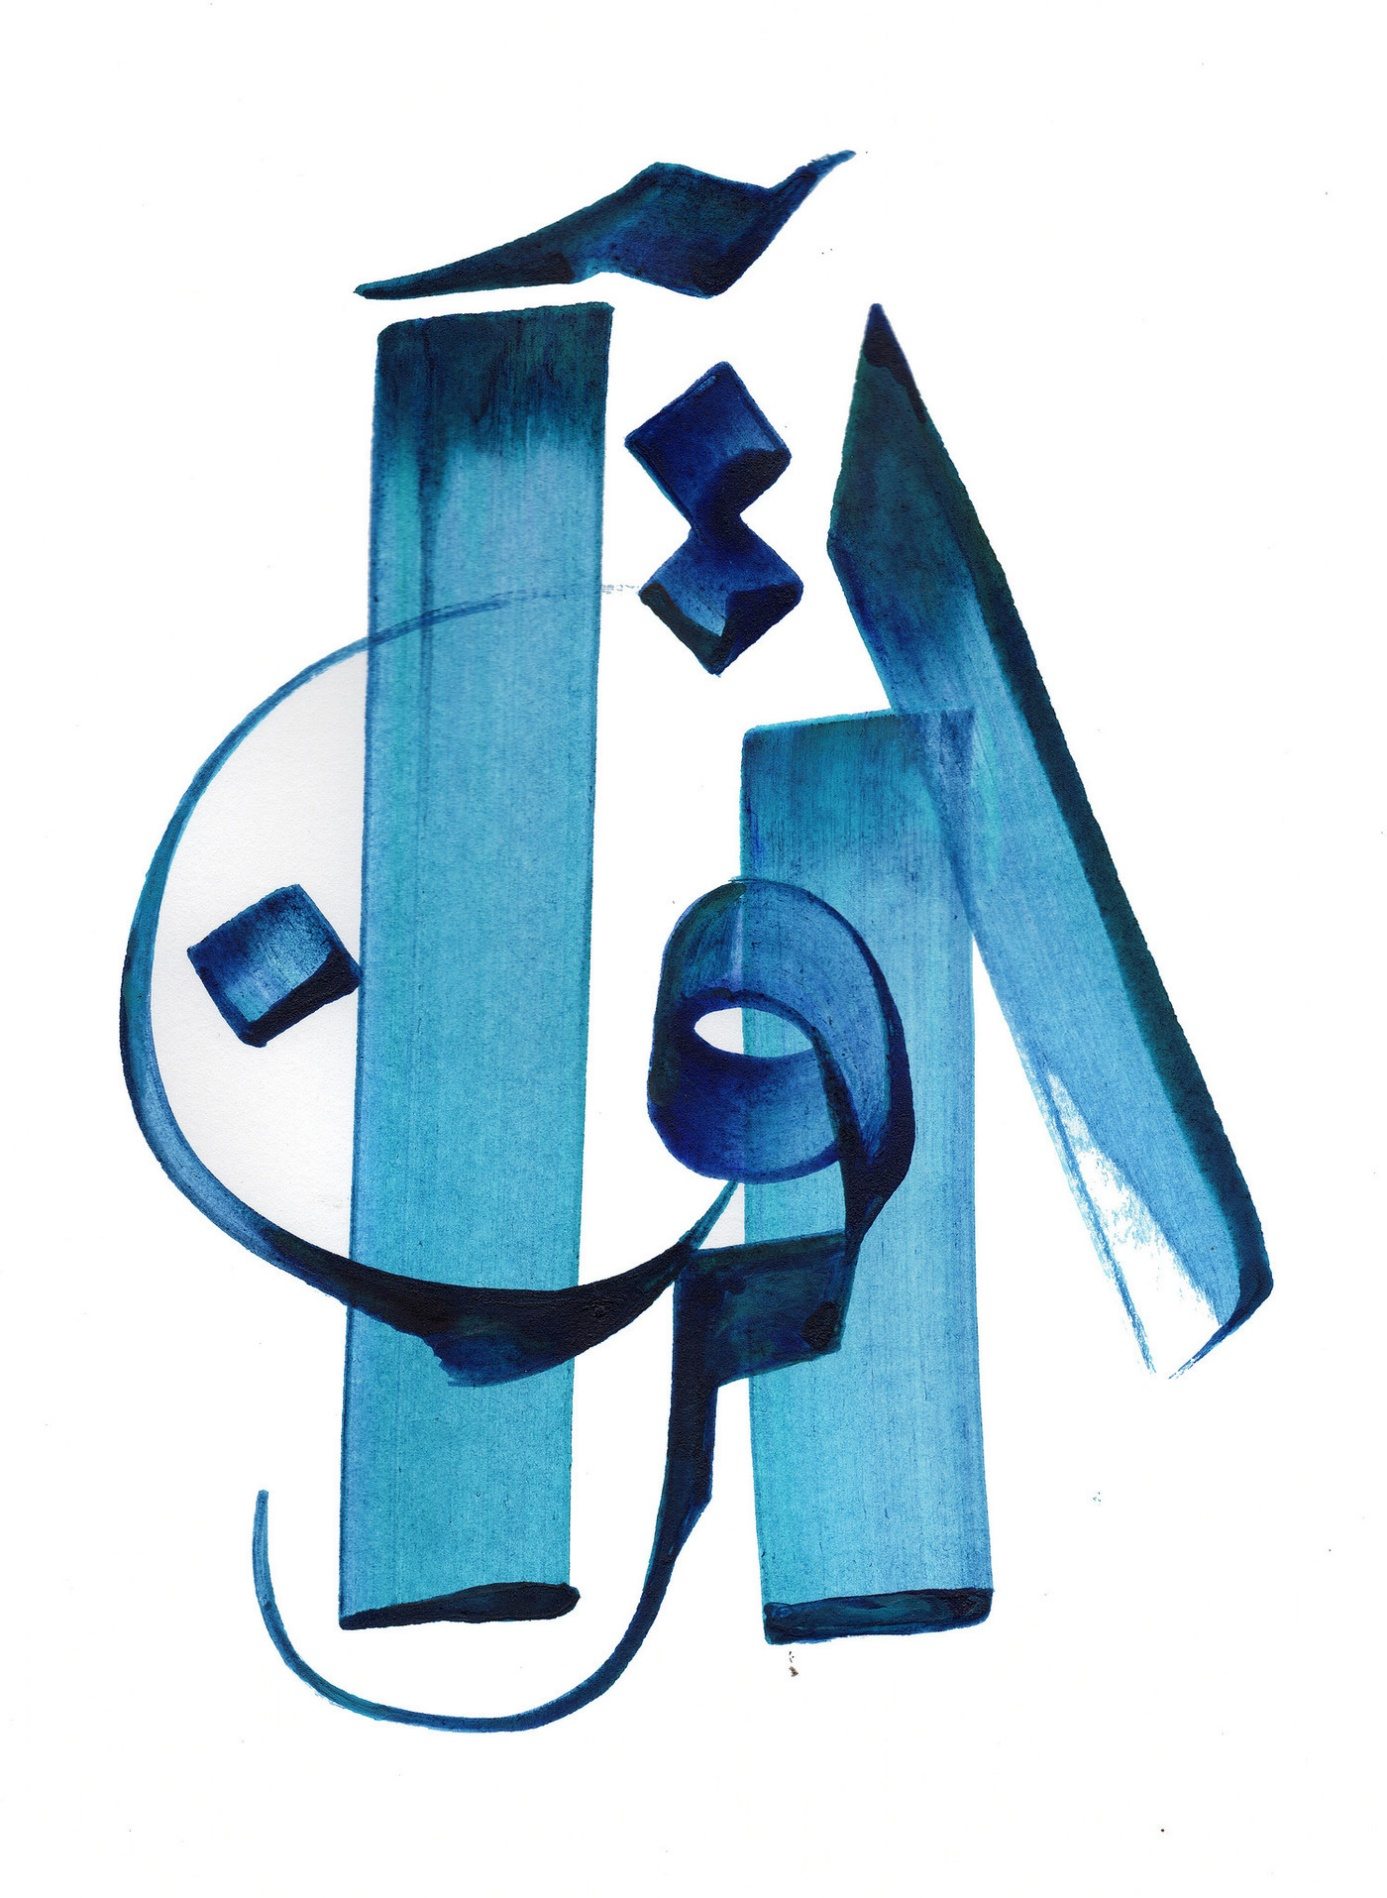
\includegraphics[width=\textwidth]{Images/image017.jpg}


\paragraph{Le regard de Hassan Massoudy}
\begin{cite}
« J'ai calligraphié le mot Coran autour de deux lignes droites,
verticales, qui forment comme l'architecture du mot. Elles lui donnent
une solidité. Avec ces deux axes, on se sent sécurisé. Ils supportent
tranquillement les autres lettres qui les chevauchent. Au centre de la
composition, une lettre forme comme un œil. Ici c'est la
lettre~\emph{qaf}-- pour le ``c'' de Coran --, qui est similaire à la
lettre~\emph{waw}. Lors d'un voyage en Turquie, j'ai découvert que les
soufis utilisaient la lettre~\emph{waw}~pour invoquer Dieu. C'est la
seule lettre de l'alphabet arabe qui, prise toute seule, peut signifier
quelque chose. Elle désigne donc l'Unique, mais sert aussi pour la
conjonction ``et''. Cette lettre évoque donc à la fois l'unique et le
multiple. »
\end{cite}



\section{Qu'est-ce que le Coran~?
}

Un livre~sacré ? Des prescriptions ? Des récits bibliques mais sans
ordre chronologique~? Que dit-il~? Comment est-il structuré~?

Avant d'exposer le Coran à la lumière de la foi musulmane, tel que les
théologiens, mystiques ou grands commentateurs l'ont compris, je vous
propose d'ouvrir quelques ouvrages récents écrits par des musulmans sur
le Coran. Ils donnent une première idée de ce que des musulmans disent
de lui et comment ils le voient.

\paragraph{Le Doute en Islam}. Le mot "islam" déjà, est l'antonyme même du doute. En effet, douter en Allah et en son Prophète est le reniement même de l'islam. Pourtant, dans la spiritualité musulmane, on peut parfois douter de soi-même et de sa capacité de croire et d'assimiler le bon et le vrai message. On peut aussi douter des interprétations et des constructions des uns et des autres mais jamais du Coran en tant que Parole révélée au Prophète. 
La seule école théologique qui, en terme de méthode, reconnaît que le "bon doute" pourrait contribuer au mûrissement de la foi, est celle rationaliste, le mo'tazilisme.  Grâce à l'esprit critique, les adeptes d'un tel courant exige de pratiquer le doute vis à vis des dogmes et des pratiques afin d'éviter tout assentiment aveugle et passif. 
Depuis Mohammad Arkoun (1928-2010) et ses héritiers, des exégètes et des historiens musulmans essaient en appliquant la méthode historico-critique  de "déconstruire" le dogmatisme régnant dans l'islam fondamentaliste.

\paragraph{Du côté des sheikh}

\begin{Def}[Sheikh]
un sheikh, c'est un sage, un homme
doué de connaissances religieuses et scientifiques reconnues. En arabe,
cela veut dire maître,
vieillard.
\end{Def}
\label{un-sheik}
Le célèbre sheikh syrien \textbf{ʿAlī Ṭanṭāwī} \sn{voir p. \pageref{theo:AliAlTawani}}, (1909-1999) écrit dans
son livre \emph{Connaître l'islam} :

  


\begin{quote}
    

«~Le musulman croit que le Coran est la parole de Dieu, apportée par
Gabriel à Muḥammad, qui l'a transmise comme il l'a entendue. Le musulman
ajoute foi que le contenu du Livre (Al-Mushâfe) dont nous disposons est
la totalité du Coran. Quiconque en nie une partie ou en doute sort de
l'Islâm.

Le Coran est le miracle de Muḥammad.

Le caractère inimitable du Coran est un fait, mais ne cherchez pas comme
les spécialistes de la rhétorique, les endroits inimitables du Coran. En
effet, ce qui est inimitable, ce ne sont pas seulement ses expressions,
ni son contenu métaphysique, mais sa globalité. Il est semblable à une
jolie femme. Sa beauté n'est pas dans la seule couleur de sa peau, dans
ses yeux, ou dans une seule partie d'elle, mais elle se trouve dans son
ensemble. Même si chaque observateur du Coran aperçoit le caractère
inimitable du côté qu'il observe.
 
{[}Muḥammad{]} a apporté un livre d'un style littéraire splendide ; au
sommet de la complétude en matière de droit ; en métaphysique il
contient des choses ignorées des hommes que la raison humaine ne peut
saisir d'elle-même~»
\mn{Tantâwî, \emph{Connaître l'islâm}.
  Citations respectives: p. 220, 241, 243, 242, cité par Anne-Sylvie
  Boisliveau, \emph{Le Coran par lui-même}, Brill, 2014.}.
  
\end{quote}



\paragraph{Du côté des prédicateurs-missionnaires~:
}

Ahmad von Denffer (né en 1948), membre de la \emph{Fondation islamique}
et auteur d'un ouvrage sur les sciences coraniques, donne la définition
suivante~:
\begin{quote}
    

«~Le Coran contient les révélations d'Allāh, le Créateur et Maître de
l'Univers, à l'humanité~». Il est «~la parole d'Allāh, descendue sur le
dernier Prophète Muhammad par l'ange Gabriel, dans un sens et une
formulation précis, transmis par de nombreuses personnes (tawātur), à la
fois par oral et par écrit. Il est inimitable et unique, protégé par
Dieu de la corruption~»\mn{~Ahmad Von Denffer, \emph{`Ulūm
  al-Qur'ān. An Introduction to the Sciences of the Qur'ān}, The Islamic
  Foundation, 1988, p. 7~; 17.}.
\end{quote}
Harun Yahya (né en 1956), créationniste musulman, dans \emph{Des secrets
du Coran,} voit dans le Coran le livre qui contient toutes les vérités.
Il donne, dit-il, les secrets de l'humanité. Tous les résultats de la
science sont déjà inscrits dans le Coran, preuve de sa puissance. Il
écrit~en introduction~:
\begin{quote}
    

«~Le Coran fournit la connaissance véridique à l'homme et contient les
secrets de la création de Dieu dans sa forme la plus vraie et la plus
pure. Toute information non fondée sur le Coran et qui est en
contradiction avec ses versets est un leurre et une illusion. Par
conséquent, ceux qui n'adhèrent pas au Coran vivent dans un état
d'hallucination ici-bas et seront condamnés au châtiment éternel dans
l'au-delà. En dehors des prières, des ordres, des interdits et des
critères moraux élevés qui sont décrits dans le Coran, Dieu communique
beaucoup de secrets à l'humanité. Un œil attentif peut en témoigner
pendant toute sa vie~»\mn{Harun Yahya, \emph{Des secrets du
  Coran}, p. 9.}.
\end{quote}




\paragraph{Du côté des nouveaux penseurs~:
}

Ghaleb Bencheikh (né en 1960) dans son livre \emph{Le Coran} écrit~:
\begin{quote}
    

«~Formulé dans sa dimension la plus traditionnelle, le Coran est le
recueil des locutions divines révélées au prophète Muḥammad Ibn Abdallah
et transmises par l'ange Gabriel sur une période de vingt-trois années
lunaires~»
\end{quote}
Puis il ajoute~:
\begin{quote}
«~Plusieurs disciplines sont requises si l'on veut véritablement étudier
le Coran pour mieux l'appréhender, s'en emparer et en faire l'exégèse.
Différentes branches des sciences humaines et de l'étude des
civilisations concourent aux multiples axes autour desquels s'articule
la recherche herméneutique contemporaine. Elle s'appuie entre autres sur
la sémiotique, la médiologie la linguistique, la philologie, l'anagogie,
la paléographie et l'historiographie~»\mn{Ghaleb Bencheikh,
  \emph{Le Coran}, Paris, Eyrolles, 2010, p. 8-10.}.
\end{quote}
Ici, le philosophe souligne la nécessité d'intégrer le recours des
données des sciences humaines pour comprendre et interpréter le Coran.
Les seules sciences islamiques traditionnelles ne suffisent plus ou plus
exactement elles enferment le Coran dans une interprétation.

\paragraph{Mohammad Arkoun} \label{Theol:Arkoun4} (1928-2010) dans son ouvrage \emph{Lectures du
Coran}, note que
\sn{Mohammed Arkoun,
  \emph{Lectures du Coran}, Paris, Maisonneuve, 1982, p. 1. \vskip 0.1cm
 Voir p. \pageref{theol:Arkoun3} }

\begin{quote}
«~pour un esprit moderne habitué à suivre une démonstration, une
évocation, une description, un récit dans des textes composés selon un
plan rigoureux, le Coran est particulièrement rebutant par sa
présentation désordonnée, son usage inhabituel du discours, l'abondance
de ses allusions légendaires, historiques, géographiques, religieuses,
ses répétitions, ses inconséquences~».
\end{quote}
Ces différents musulmans présentent d'une manière particulière le Coran,
donnant un éclairage singulier.
Bien que ces penseurs musulmans contemporains soient minoritaires, ils restent les pionniers de la production intellectuelle musulmane actuelle et l'actualisation de la doctrine islamique à la lumière des sciences humaines et sociales modernes. Même si une partie de l'imaginaire musulman actuel reste sous l'influence des écoles juridiques fondamentalistes, ces penseurs modernes sont très appréciés et écoutés par les musulman libéraux surtout ainsi qu'auprès des non-musulmans engagés dans le dialogue inter-religieux.   
Pour les plus intégristes, ils sont considérés comme \textit{zanadiqa}, hérétiques, blasphémateurs ou coupable d'apostasie. Et il ne faut pas oublier que, le blasphème est toujours puni de mort dans plusieurs pays islamiques.... En revanche, condamner à mort un penseur musulman reste un fait rare. Junaid Hafeez, par exemple, professeur d’université au Pakistan, était emprisonné depuis six ans quand il a été condamné à mort en décembre 2019 pour blasphème. Sa condamnation fait aujourd'hui l'objet d'un appel. A suivre ! Avec la prison, ils pourraient être interdits d'enseigner ou de se rendre dans des pays musulmans. On peut surtout aussi mettre sur l'Index leurs publications. L'Arabie Saoudite interdit l'ouvrage "Le Coran et ses lectures" d'Abdelmajid Charfi. 

Quoique dans le contexte actuel, l’islamisme considère que la critique du Prophète et sa représentation est l' acte le plus grave qui mérite le plus dur des châtiments, la critique de la Sunna pourrait être elle aussi compromise. Mais, il ne faut pas oublier, qu'actuellement en France, des penseurs musulmans contemporains qui n'hésitent pas de poursuivre leur méthode historico-critique. 

 Pour un premier approfondissement, il
convient de revenir à la méthode des savants de l'islam et de partir de
l'étymologie.

\vide{uxe9tymologie}{%
\subsection{Étymologie}\label{uxe9tymologie}}

La racine \emph{qara'a} signifie lire à haute voix, réciter. Par suite,
le \emph{Qur'ān} est une lecture. L'étymologie peut surprendre puisque
le \emph{Qur'ān}, avant d'être un livre, est donc une récitation d'un
livre. Pour les musulmans, cette récitation suscite une capacité
d'émotion religieuse bouleversante. Le Coran ne se lit pas, mais se
récite, se psalmodie. Il existe des règles précises et l'ensemble de ces
règles correspond au \emph{taǧwīd}. Le mot vient de la racine ǦaWaDa qui
signifie améliorer, rendre meilleur. On le distingue du \emph{tartīl}
qui est la lecture lente du Coran.

Les mosquées organisent parfois des concours de \emph{taǧwīd},
récitation du Coran, pour les enfants. C'est sur le principe de
\emph{The Voice}, avec un jury. Mais il note le participant en fonction
du respect des règles sur les pauses, les syllabes allongées, etc. Tout
y est beaucoup moins subjectif. Dans le film \emph{Wajda}, de 2012, qui
raconte avec beaucoup d'humour l'histoire d'une jeune enfant saoudienne
qui rêve d'avoir un vélo, on la voit dès les premières scènes du film
dans une école coranique où elle apprend le Coran. L'apprentissage du
Coran n'est pas réservé aux seuls hommes~! Pour autant, le film est très
ironique car en déplaçant bien des problématiques d'adultes dans le
monde de l'enfance, il n'en dessine pas moins un triste tableau de la
condition des femmes en Arabie. A son camarade, Wajda dit qu'elle veut
faire du vélo avec lui, mais lui de lui répondre~: «~ce n'est pas
possible, tu es une femme~». Et elle de renchérir~: «~tu dis ça, parce
que tu sais que si je faisais du vélo je serai meilleure que toi~».

\vide{section-13}{%
\subsubsection{}\label{section-13}}

\vide{extrait-de-la-ruxe9citation-coranique-par-un-iranien-de-7-ans-devant-un-public-manifestement-conquis-uxe9coutez-jusquuxe0-la-fin.}{%
\mn{{Extrait de la récitation coranique par un
iranien de 7 ans devant un public manifestement conquis\ldots{} écoutez
jusqu'à la fin.
}{Extrait de la récitation coranique par un iranien de 7 ans devant un public manifestement conquis\ldots{} écoutez jusqu'à la fin. }}\label{extrait-de-la-ruxe9citation-coranique-par-un-iranien-de-7-ans-devant-un-public-manifestement-conquis-uxe9coutez-jusquuxe0-la-fin.}}

Cette puissance affective ou émotionnelle de la récitation coranique est
affirmée par le Coran lui-même~:
\begin{quote}
    
«~Il dit de lui-même que cette lecture est splendide~: «~Dis~:
`croyez-le ou ne le croyez pas, à ceux à qui le savoir a été donné avant
cela, lorsque l'on leur récite {[}le Coran{]}, ils tombent prosternés
sur leurs faces~» (S. 17, 107).

\TArabe{قُلْ آَمِنُوا بِهِ أَوْ لَا تُؤْمِنُوا إِنَّ الَّذِينَ أُوتُوا
الْعِلْمَ مِنْ قَبْلِهِ إِذَا يُتْلَى عَلَيْهِمْ يَخِرُّونَ
لِلْأَذْقَانِ سُجَّدًا}

\end{quote}

Mais avant de poursuivre sur la manière dont le Coran parle de lui-même,
il importe de décrire le livre, de découvrir sa structure, sa
composition.

\vide{composition-et-structure-du-coran}{%
\section{1.~Composition et structure du
Coran}\label{composition-et-structure-du-coran}}

\vide{un-livre-formuxe9-de-sourates}{%
\subsection{{1.1 Un livre formé de sourates
}{1.1 Un livre formé de sourates }}\label{un-livre-formuxe9-de-sourates}}

\vide{terminologie-et-nombre-des-sourates}{%
\subsubsection{1.1.1 Terminologie et nombre des
sourates}\label{terminologie-et-nombre-des-sourates}}

Le Coran est composé de 114 sourates, ordonnées de la plus longue à la
plus courte -- comme pour les épîtres de Paul -- à l'exception de la
première qui s'apparente à une prière introductive. Nous reviendrons sur
cette première sourate qui s'apparente très étrangement au Psaume
1\textsuperscript{er}. L'ouverture du Coran, comme l'ouverture du
Psautier~? C'est bien ce que je dis. Et une analyse intertextuelle le
prouve. Ouvrez l'un et l'autre et regardez, comparez.
\mn{Comparaison entre le Ps 1 et la sourate \textit{Al-Fatiha (L'ouverture)}}
\begin{longtable}{p{4.2cm}p{4.2cm}p{3cm}}
\toprule
Ps 1 & Al-Fatiha (L'ouverture) &\TArabe{ سورة الفاتحة }\\
\midrule
\endhead
& Au nom d'Allah, le Tout Miséricordieux, le Très Miséricordieux.

Louange à Allah, Seigneur de l'univers.

Le Tout Miséricordieux, le Très Miséricordieux, &\TArabe{ بِسْمِ اللَّهِ
الرَّحْمَنِ الرَّحِيمِ

2 الْحَمْدُ لِلَّهِ رَبِّ الْعَالَمِينَ

3 الرَّحْمَنِ الرَّحِيمِ }\\
{1. Heureux l'homme qui ne marche pas selon le conseil des
méchants, Qui ne s'arrête pas sur la voie des pécheurs, Et qui ne
s'assied pas en compagnie des moqueurs,} & & \\
{2. Mais qui trouve son plaisir dans la loi de l'Eternel, Et qui la
médite jour et nuit!} & & \\
{3. Il est comme un arbre planté près d'un courant d'eau, Qui donne
son fruit en sa saison, Et dont le feuillage ne se flétrit point: Tout
ce qu'il fait lui réussit.} & & \\
{4. Il n'en est pas ainsi des méchants: Ils sont comme la paille
que le vent dissipe.} & & \\
{5. C'est pourquoi les méchants ne résistent pas au} jour du
jugement\textbf{, Ni les pécheurs dans l'assemblée des justes;} &
4.Maître du \textbf{Jour de la rétribution.}

C'est Toi {[}Seul{]} que nous adorons, et c'est Toi {[}Seul{]} dont nous
implorons secours. &\TArabe{ 4 مَالِكِ يَوْمِ الدِّينِ

5 إِيَّاكَ نَعْبُدُ وَإِيَّاكَ نَسْتَعِينُ }\\
{6. Car l'Eternel connaît la} voie des justes\textbf{, Et la voie
des} pécheurs mène à la ruine\textbf{.} & Guide-nous dans le
\textbf{droit chemin,}

\textbf{le chemin de ceux que Tu as comblés de faveurs}, non pas de ceux
qui ont encouru Ta colère, ni \textbf{des égarés}. &\TArabe{ 6 اهْدِنَا
الصِّرَاطَ الْمُسْتَقِيمَ

7 صِرَاطَ الَّذِينَ أَنْعَمْتَ عَلَيْهِمْ غَيْرِ الْمَغْضُوبِ عَلَيْهِمْ
وَلَا الضَّالِّينَ }\\
\bottomrule

\end{longtable}

\begin{Def}[āyat]
Chaque sourate (\emph{sūra}) est composée de versets (\emph{āyah},
\emph{āyat}) mot qui signifie au préalable signe~: chaque verset est en
lui-même un signe donné par Dieu
\end{Def}


\vide{on-retrouve-ce-mot-dans-ayatollah-qui-veut-donc-dire-signe-de-dieu}{%
\mn{on retrouve ce mot dans ayatollah, qui veut donc
dire~\ldots{} signe de
dieu}\label{on-retrouve-ce-mot-dans-ayatollah-qui-veut-donc-dire-signe-de-dieu}}

 Selon les lexicographes, \emph{āyah} renvoie à l'idée de merveille, de
prodige. Le mot souligne la dimension prophétique et prodigieuse du
signe transmis à Muḥammad.

Le terme de sourate (\emph{sūrat}) apparaît à neuf reprises dans le
coran au singulier et une fois au pluriel. Sa signification reste
confuse. Les lexicographes remarquent qu'il provient de la racine SWR
qui signifie monter sur un mur, se hisser sur, assaillir, fondre sur
quelqu'un, être impétueux\sn{~\textsc{Gloton}, \emph{Lexique},
  n°0756, p. 466. Voir aussi Roger \textsc{Arnaldez}, \emph{Le Coran,
  Guide de lecture}, Paris, Desclée, 1983, p. 36.}. \emph{Sūrat}
signifie à la fois rangée de pierre, trace, indication, signe. Chez le
commentateur \textbf{Faḫr al-Dīn al-Rāzī}.


{c'est encore un nom nouveau, mais on ne peut parler du
Coran sans très vite parler d'al-Rāzī. Il est en effet l'auteur d'un des
plus sublimes commentaires du Coran, \emph{Les clefs de l'invisible}.C'est un Persan du XII\textsuperscript{e} siècle.}
\sn{Michel Lagarde
  a consacré une belle étude sur ce Commentaire~: Michel
  \textsc{Lagarde}, \emph{Les secrets de l'invisible : Essai sur le
  Grand Commentaire de Fahr al-Dîn al-Râzî}, Paris, Albouraq, 2009.}. 

on trouve l'idée selon laquelle de même qu'une muraille entoure une
ville de tout ce qu'elle contient, de même la \textbf{sourate enveloppe
la science contenue dans le Coran}. L'idée de mur ou de muraille est
aussi interprétée comme signifiant l'élévation du croyant qui
s'approprie l'enseignement du Coran~: c'est l'interprétation donnée par
\textbf{Qurṭubī} (1214-1273), autre grand exégète du Coran.

Mais pourquoi y a-t-il des sourates~? Pourquoi le Coran n'est-il pas
écrit en un seul bloc~? Pourquoi donc une composition~de plusieurs
éléments ? Cette question est typique de celles que l'on trouve dans le
commentaire de \textbf{Faḫr al-Dīn al-Rāzī} où il se demande
systématiquement pourquoi les choses sont ainsi et pas autrement~:
pourquoi telle construction grammaticale, pourquoi tel mot sous telle
forme, pourquoi tel ordre et ici, pourquoi des sourates et pas tout
simplement un Livre en un seul tout\textbf{.} \mn{Roger Arnaldez expose la
réponse d'al-Rāzī dans son livre \emph{Le Coran Guide de lecture}.}

\vide{nom-des-sourates}{%
\subsubsection{{Nom des sourates
}}\label{nom-des-sourates}}

Chaque sourate est désignée par un nom. Cette désignation semble tardive
puisque les compagnons de Muḥammad à La Mecque rapportent des versets
des sourates à partir de leurs noms. Le nom des sourates dépend d'un
thème ou d'un élément cité dans la sourate. Ainsi, par exemple, la
sourate al-Tawba porte sur le repentir accueilli par Dieu à Muḥammad, à
ceux qui étaient avec lui et à ceux qui étaient restés derrière lui. Il
y a quelques étrangetés, comme le nom de la Sourate
2\textsuperscript{e}, la Vache, \emph{al-Baqara}. Le thème est tiré des
Nombres et du Deutéronome en lien avec Moïse. Or, l'épisode de la vache
ne couvre que huit versets sur 286 (versets 67-73).

\vide{nature-des-sourates}{%
\subsubsection{Nature des sourates}\label{nature-des-sourates}}

Certaines sourates sont très particulières : la première sourate par
exemple, al-Fātiḥa, l'Ouvrante, est une prière adressée à Dieu par les
croyants. Elle illustre parfaitement l'élaboration progressive du texte
coranique : on en a trouvé des variantes textuelles dans des traditions
ou des ouvrages anciens. Une teneur identique, mais des mots, des
constructions syntaxiques différentes.

La sourate 111 (\emph{al-masad}, la corde) est une formule de
malédiction de type archaïque. Rien dans le texte ne spécifie ce dont il
s'agit. Il est donc une énigme. Les circonstances de la Révélation
diront plus tard qu'il s'agit d'une malédiction prononcée par Muhammad
contre un de ses oncles hostile à sa prédication. Nous avons déjà
rencontré son nom. Ce serait Abū Lahab.

Les deux dernières sourates sont des incantations magico-prophylactiques
(pour préserver la santé). Elles semblent avoir suscité bien des litiges
quant à leur insertion.

Le Coran comporte des proclamations oraculaires (comme les oracles qui
rapportent ce qu'ils voient), des hymnes sous une forme poétique :
l'évocation poétique du Paradis est une adaptation arabe originale des
Hymnes d'Ephrem de Nisibie, Père de l'Église syriaque (+ 373). Oui, les
versets eschatologiques sur les houris sont des échos des hymnes de St
Ephrem. Sur ce point, les travaux d'intertextualité d'Andrae Tor sont
une référence incontournable et plus récemment de Christoph
Luemberg\sn{Tor Andrae, \emph{Les origines de l'islam et le
  christianisme}, Paris, 1955.
\sn{
   le compte-rendu de ce livre dans la Revue d'histoire des
  religions
  \url{http://www.persee.fr/doc/rhr\_0035-1423\_1957\_num\_151\_2\_8712}.}.}

Il y a des récits, des textes législatifs et parénétiques (exhortatifs).
On y trouve aussi des discours de guerre, d'appel au combat
(\emph{ğihād} ou \emph{qitāl})\sn{Emmanuel \textsc{Pisani}, «~La
  violence dans le Coran~», sur le site~:
  \url{http://www.croire.com}{www.croire.com} , juin 2015.}. Cette
guerre est contre plusieurs ennemis : les gens du Livre qui ne
pratiquent pas la religion de la vérité (S. 9, 111).

Il y a aussi des discours polémiques~: Mehdi Azaiez, - il a consacré sa
thèse de doctorat à l'analyse de ce genre littéraire dans le Coran -,
remarque qu'il s'agit de «~l'un des genres les plus marquants du corpus
coranique~»\sn{Medhi \textsc{Azaiez}, «~Le contre-discours
  coranique. Premières approches d'un corpus~», dans Azaiez,
  \emph{Nouvelles approches du} Coran, Paris, CNRS, 2013, p 257.}. On
trouve ainsi cette invitation à «~débattre de la meilleure
façon~»~(S.16, 125)\sn{~Jane Dammen \textsc{McAuliffe}, «~Debate
  with them in a better Way : the Construction of a Qur'anic
  Commonplace~», dans \emph{Myths, historical archetypes and symbolic
  figures in Arabic literature towards a new hermeneutic approach},
  Proceedings of the International Symposium in Beirut, June 25th-June
  30th, 1996, / Edited by Angelika Neuwirth, Birgit Embaló, Sebastian
  Günther, 1999, p. 163-188.} :
\begin{quote}
    
«~Appelle les hommes dans le chemin de ton Seigneur par la sagesse et
une belle exhortation~; discute avec eux de la meilleure manière~»

\TArabe{ادْعُ إِلَى سَبِيلِ رَبِّكَ بِالْحِكْمَةِ وَالْمَوْعِظَةِ
الْحَسَنَةِ وَجَادِلْهُمْ بِالَّتِي هِيَ أَحْسَنُ إِنَّ رَبَّكَ هُوَ
أَعْلَمُ بِمَنْ ضَلَّ عَنْ سَبِيلِهِ وَهُوَ أَعْلَمُ بِالْمُهْتَدِينَ}
\end{quote}

Il fait remarquer que la polémique est inhérente à l'islam originel dans
la mesure où la parole de Muḥammad a d'abord été rejetée par le groupe
tribal auquel il appartenait. C'est donc avec les siens qu'il a fallu
d'abord débattre et convaincre si bien que la question de la polémique
émerge dès la naissance de l'islam. Les débats, les réponses formulées
aux contradictions sont inhérents au texte et peuvent se traduire par
des incantations, des malédictions, des reproches, des avertissements,
des railleries, des apostrophes en direction des
non-croyants\sn{Neal \textsc{Robinson}, \emph{Discovering the
  Qur'an}, p. 116, cité par Azaiez, \emph{op. cit}., p. 259.}.

\vide{agencement-des-sourates}{%
\subsubsection{{Agencement des sourates
}}\label{agencement-des-sourates}}

Autre question, celle de l'agencement des sourates et l'ordre des
versets. Quel ordre suivre~? Cette question est au cœur d'une
\emph{disputatio} entre les savants musulmans.

L'exégète al-Qurṭubī (nous avons déjà rencontré ce noms avec al-Rāzī)
rapporte les propos du Qāḍī Abū Bakr Ibn Al-Ṭayyib~: «~On peut faire
l'objection que les Anciens ont été en désaccord sur l'ordre des
sourates du Coran. Certains, dans leur recueil, ont écrit les sourates
selon la chronologie de leur révélation, et ils ont mis en tête les
sourates mecquoises, puis les sourates médinoises~; certains commencent
par la louange al-Ḥamd, d'autres par la sourate 96~: `Récite, au nom de
ton Seigneur qui créa\ldots'~: tel est le début du recueil de `Alī.
Quant à celui d'Ibn Mas`ūd, il commence par `Maître du Jour du Jugement
(1,3), puis viennent la sourate \emph{La Vache} (2) et la sourate
\emph{Les femmes} (4)\ldots{} Le recueil d'Ubayy débute par al-Ḥamd~;
suivent les sourates 3, La Famille de `Imrān la sourate 6, les
Troupeaux, la sourate 7, al-`Araf, la sourate 5, La Table et ainsi de
suite\ldots{} avec de profondes divergences~»\sn{Cité par
  \textsc{Arnaldez}, \emph{Le Coran. Guide de lecture}, \emph{op. cit}.,
  p. 47.}.

L'exégète ici se fait l'écho d'un débat quant à l'agencement des
sourates au sein même de la tradition musulmane. La découverte d'anciens
manuscrits du Coran à San`ā au Yémen, en 1972 confirme l'existence de
différents corpus coraniques. Muḥammad Amir Moezzi \mn{Voir aussi pour un détail de l'approche historico-critique \cite{Amir:CoranHistoriens} }écrit~à ce propos~:
\begin{quote}
    «~En sus de quelques variantes orthographiques et lexicographiques
mineures, 22\% des 926 groupes de fragments étudiés présentent un ordre
de succession de sourates complètement différent de l'ordre connu~: le
découpage en versets ne correspond à aucun des 21 systèmes connus. Ce
qui est frappant c'est que l'ordre des sourates se rapproche le plus des
codex d'Ubbay et d'Ibn Mas`ūd~»\sn{\textsc{Cuypers, Gobillot},
  \emph{Idées reçues}, p. 18.}.
\end{quote}


Il semble donc qu'existèrent entre ces recensions des différences, à la
fois dans l'ordre, mais aussi dans le texte. Mais retenez aussi que la
tradition musulmane rapporte l'existence de différents corpus~: elle les
canonise d'une certaine façon. Parmi ces corpus, la tradition sunnite
reconnaît que `Alī avait élaboré son corpus\ldots{} Corpus dans lequel
serait inscrit, d'après la tradition šī`ite, les versets divins qui
désignaient `Alī comme successeur de Muḥammad\ldots{}

 
\subsection{ Un livre en arabe clair} 
\begin{quote}
    
«~Voici un Livre dont les versets sont clairement exposés~; un Coran
arabe, destiné à un peuple qui comprend~» (S.~41, 2-3).
\end{quote}

Et le Coran de préciser «~un arabe clair (\emph{`arabiyyun mubīn})~» (S.
16, 103 et 26, 195).

Le Coran de lui-même accorde une importance singulière à la langue
arabe. On comprend pourquoi, face à une question, il convient de revenir
aux mots arabes et à leur signification.

L'arabe est comme magnifié. Mais cet arabe est-il si clair~comme
l'affirme le Coran ? Et s'il l'est, pourquoi tant de niveaux de
commentaires, et d'explications parfois contradictoires~? Pourquoi le
prophète Muḥammad a-t-il dû expliquer les significations du Coran à ses
compagnons~? Quel crédit et quelle autorité accorder aux explications
propres aux compagnons~eux-mêmes ? Ces questions nous introduisent dans
une des difficultés propres à tout texte sacré et qui est sa
compréhension. Comme le dit Tariq Oubrou, imam de Bordeaux, «~il ne
suffit pas de lire le Coran pour le comprendre~».


\section{Histoire du Coran~: sa constitution
(\emph{muṣḥaf})}

Depuis quand le Coran existe-t-il sous la forme qui est la sienne
aujourd'hui~? Muḥammad a-t-il eu de son vivant et sous ses yeux le texte
coranique tel qu'il est structuré~? Il n'en est rien et la constitution
du \emph{muṣḥaf}, c'est-à-dire le Coran dans sa matérialité, n'est pas
effective avant la fin du premier siècle de l'Hégire. Elle souligne que
l'islam s'inscrit pleinement dans la tradition de l'oralité, et avant
d'être un livre, le Coran était une récitation. Mais pourquoi a-t-on
éprouvé le besoin de rassembler les sourates en un livre~? Tel est
l'objet de la présente partie.

 
\subsection{L'initiative d'Abū Bakr
} 

Selon la tradition, à la mort de Muḥammad, en 632, la Révélation est
connue par cœur et dans son intégralité par quelques rares fidèles qui
sont appelés les lecteurs du Coran (\emph{qurrā'} -- on retrouve la
racine QR' comme dans \emph{Qur'ān}, Coran). Leurs noms divergent selon
les traditions. Mais le Coran comme \emph{muṣḥaf} n'existe pas encore.

À la mort de Muḥammad, Musaylima, celui qui se prétendait aussi prophète
et qui a écrit une lettre à Muḥammad -- épisode de la Sīra que nous
avons rencontré dans le précédent chapitre -- jouissait d'une certaine
aura. Le voici qui vient trouver Abū Bakr, le premier successeur de
Muḥammad, le premier calife donc, et affirme : «~Gabriel est venu me
trouver et m'a confié la mission de prophète par toute la terre~». Il
s'insurge contre le calife et met en déroute le premier général envoyé.
En l'année 633, Abū Bakr charge Ḫālid Ibn al-Walīd de mettre un terme
aux agissements de Musaylima. C'est la bataille de `Aqrabā. Il y trouva
la mort.

Cependant, au cours de la bataille, de nombreux récitants
(\emph{qurrā'}) trouvèrent aussi la mort. `Umar aurait pris conscience
du risque de perdre des fragments du Coran. Il en informe le calife Abū
Bakr qui charge Zayd Ibn Thabit de rassembler les sourates sur des
feuilles. La tradition est rapportée ainsi par Buḫarī dans la
\emph{Sunna}, au Livre 66, chapitre 3.
\begin{quote}
    
«~Zayd ibn Ṯābit a dit~: «~Abū Bakr vint me faire chercher à la suite du
massacre des gens de Yamāma. Lors {[}de ma venue{]} je trouvai Abū Bakr
chez lui et il me dit~: `Umar vient de m'informer que le massacre qui
eut lieu à Yamama a mis fin à la vie de lecteurs du Coran et je crains
que si le combat devait perdurer, ils continuent de se faire tuer sur
les champs de bataille, si bien que disparaîtrait une bonne partie du
Coran. C'est pourquoi je pense qu'il te faut collectionner le Coran'\,'.
J'ai alors dit à `Umar : `Comment vas-tu faire quelque chose que le
Messager d'Allah n'a pas faite~?'\,' -- `Umar dit~: Par Allāh,~ceci est
une bonne chose ». Il ne cessa de me répéter son idée jusqu'à ce
qu'Allāh m'ouvrit le cœur et me fit adhérer à ce qu'\,`Umar avait
proposé.~»

\mn{ Vous avez lu que je vous ai parlé de la
bataille de `Aqarbā, mais la tradition parle des gens de Yamāma\ldots{}
alors~? En fait, `Aqrabā est le nom d'une plaine de la région de Yamāma.
J'ajouterai aussi que d'après la tradition musulmane, Abū Bakr avait
envoyé 3000 hommes~! Ce qui veut dire aussi que Musaylima avait des
disciples et nombreux étaient aussi ceux qui suivaient ses prophéties.
La région semble connaître un embrasement prophétique. a bataille
d'Al-Yamama (arabe \TArabe{
اليمامة} 
)
ou bataille d'al-`Aqrabā aura eu lieu, selon
les sources musulmanes, en 633, dans le cadre des Guerres de Ridda
(l'Apostasie), sur la plaine de Aqraba dans la région d'Al-Yamama (dans
l'actuelle Arabie Saoudite) entre les forces du calife Abou Bakr le
véridique et Musaylima le menteur, un prophète autoproclamé.
}
Zayd dit~alors qu'Abū Bakr avait poursuivi en disant~: `tu es un homme
jeune, raisonnable et au-dessus de tout soupçon et tu transcrivais déjà
par écrit la révélation pour le prophète. Collecte et rassemble donc le
Coran'. Par Dieu, me disais-je, s'il m'avait mandaté pour déplacer une
montagne, cela m'aurait été plus aisé que d'exécuter l'ordre de
rassembler le Coran. Je dis : `comment allez-vous faire quelque chose
que le Messager d'Allah n'a pas faite~? Mais il (Abū Bakr) dit~: «~Par
Allāh, c'est une bonne chose.~» Et puis il ne cessa de me répéter son
idée jusqu'à ce qu'Allāh m'en inspirât l'admission comme Il l'avait fait
pour Abū Bakr et pour `Umar. Dès lors, je me suis mis à rechercher et à
collecter les éléments coraniques transcrits sur des branches de dattier
et sur des pierres lisses ou conservées dans la mémoire des gens et j'ai
trouvé les derniers versets de la sourate \emph{at-Tawba} chez Abū
Ḫuzayma al-Anṣārī que je n'avais pas trouvés chez les autres\ldots{} Les
feuilles contenant le Coran furent conservées par Abū Bakr jusqu'à sa
mort puis elles furent déposées auprès d'\,`Umar qui les garda jusqu'à
sa mort puis elles furent transférées à sa fille Ḥafṣa.
\end{quote}

De cette tradition, on peut retenir avec une certaine assurance qu'une
compilation fut entreprise à l'époque d'Abû Bakr. `Umar les accueillit
puis sa fille, Ḥafṣa.




\subsection{{La constitution de la Vulgate de `Uṯmān
}}

C'est donc sous `Uṯmān (l'impulsion vient d'Abū Bakr, mais la
constitution lui est postérieure~: il ne vécut pas assez longtemps) que
l'on entreprit la collection du Coran. Outre le récit transmis par la
tradition, l'histoire montre que cet acte est loin d'être purement et
simplement religieux. Il revêt une dimension politique~: il s'agit de
\textbf{contrebalancer le pouvoir des lecteurs qui se sont institués
gardiens du texte sacré}. Cela sert par ailleurs la politique
centralisatrice déployée par le troisième calife.

Mais si l'initiative califale permet au calife de concentrer les
pouvoirs politiques et religieux, il n'est pas le seul à vouloir
constituer une Vulgate.

 
\subsection{ La constitution d'autres corpus
} 

Ainsi, certains compagnons du Prophète, attachés à la transmission de la
Parole, vont proposer leurs propres recensions. On a ainsi parlé d'un
corpus de Sālim Ibn Ma`qil -- mais il est mort un an après le Prophète.
Plus solide, serait la recension d'un cousin de Muḥammad, `Abd Allāh Ibn
`Abbās (m. 68 / 688). Ce corpus est aujourd'hui perdu.

\mn{{`Alī} -- petit rappel~: c'est le cousin et le gendre de
Muḥammad, le premier converti à l'islam selon la \emph{Sīra} --, selon
les šī`ites, était aussi en sa possession du \emph{muṣḥaf}.}

On trouve aussi le corpus d'Abd Allāh \textbf{Ibn Mas`ūd} (m. 30 / 650),
un des premiers convertis à l'islam, très proche du Prophète. Lui aussi
va rédiger un corpus. On sait à partir de citations diverses dans des
ouvrages anciens que différentes recensions circulaient. La version
d'Ibn Mas`ūd a par exemple circulé à Koufa en Irak puisque le gouverneur
d'Irak exigea de détruire ce corpus. Or, en 1007, le même ordre fut
répété à Bagdad ce qui signifie bien qu'il n'avait pas été complètement
détruit. Cela indique aussi qu'il présentait des divergences par rapport
à la Vulgate de `Uṯmān.

Toutefois, les variantes entre les différents codex semblent avoir été
minimes. On a établi que la version de Mas`ūd ne comportait pas la
première sourate, ni les deux demandes de protections (S. 113 et 114).
On a émis l'hypothèque très plausible que ces trois sourates formaient
un encadrement liturgique qui apparemment n'étaient pas dans le Coran
primitif. Vous vous souvenez du Psaume 1 qui ouvre le Psautier\ldots{}

Dès le premier siècle, un autre débat voit le jour quant à la manière de
réciter le Coran et à la nature même des consonnes qui sont utilisées.
On a un écho de cette question dans la Sunna. \mn{voir \cite{Deroche:CoranPluriel} qui soutient une vision unifiée du Coran par Muhammad par rapport au \emph{Coran des Historiens}} En effet, certains
lecteurs lisaient en recourant à d'autres lettres ce qui entraina des
divergences de lectures. Elles étaient nombreuses entre l'Irak et en
Syrie et ils s'en suivaient des accusations d'anathèmes réciproques. Il
faut bien voir que l'écriture arabe présentait des déficiences puisque
des phonèmes différents comme b, t, ṯ, n, y, étaient écrits avec le même
signe alphabétique. De plus, les signes indiquant les voyelles n'étaient
pas inscrits ce qui orientait le texte dans des sens grammaticaux
pluriels. Par conséquent, il y avait des traditions de lectures
(\emph{qirā'āt}) différentes selon les villes et les régions. Avec les
conquêtes, l'islam était prêché dans des contrées où existaient d'autres
dialectes et surtout d'autres prononciations. Un Égyptien ne prononce
pas la lettre \emph{dji}, mais il dit \emph{gué} -- ce que ne fait pas
le Syrien. Demandez à un Arabe de prononcer la lettre p\ldots{} il ne
dira pas \emph{p}ardon, mais \emph{b}ardon.

C'est dans ce contexte que l'on a renvoyé à un \emph{ḥadīṯ} sur les
lectures du Coran. Ainsi, on trouve dans la Sunna
d'\textbf{al-Buḫarī}~-- c'est un des très grands compilateurs de l'islam
de ḥadīṯ. Son nom sera revu et revu dans le prochain chapitre.




\subsubsection{Ces 5 variantes de Harf sont un moyen de rentrer dans une
pluralité de
sens}



\begin{quote}
    «~Un jour, lors du vivant du Prophète, j'entendis Hishâm ibn Hakîm
réciter la sourate al-Furqân. Alors que j'écoutais avec attention sa
récitation, je m'aperçus qu'il recourait à certaines lettres différentes
de celles que le Prophète m'avait enseignées. Je m'apprêtais à
l'interpeller durant sa prière, mais je me retins et attendis qu'il la
terminât. Je le pris alors par son vêtement et lui dis : "Qui donc t'a
enseigné ainsi la sourate que je t'ai entendue réciter ? -- C'est le
Prophète, me répondit-il. - Tu mens, lui répliquai-je, car il me l'a
enseignée avec des lettres différentes que certaines de celles que tu
viens de réciter." Je l'emmenai alors auprès du Prophète et exposai à
celui-ci le problème : "J'ai entendu cet homme réciter la sourate
al-Furqân avec certaines lettres autres que celles que tu m'as
enseignées. -- `Laisse-le' me dit le Prophète. Puis, se tournant vers
Hishâm, il lui dit : "Récite, Hishâm." Hishâm récita alors la sourate de
la même manière qu'il l'avait faite auparavant. Le Prophète dit alors :
`Ainsi a été révélée cette sourate'. Puis il me dit : `Récite, toi,
Umar'. Je le fis alors selon la façon que lui-même m'avait enseignée. Il
dit également : `Ainsi a été révélée cette sourate'. Puis il conclut :
`Le Coran est révélé selon sept variantes de récitation (\emph{harf}).
Récitez donc celle qui est facile pour vous'\emph{~(rapporté par
al-Bukhârî, Ṣaḥih ~Book 97, Hadith 175, n° 4706)}~»\emph{.}
\end{quote}


Vous ne le saviez peut-être pas, mais il y a donc plusieurs manières de
lire le Coran, avec d'autres consonnes, et donc d'autres mots, et donc
d'autres significations. Ce \emph{ḥadīṯ} permet de mettre fin à des
divergences de lectures qui devaient être conflictuelles et de
réconcilier ainsi tous les musulmans. À l'intérieur même du texte,
l'uniformité de lecture n'est donc pas absolue. Peu à peu s'imposèrent
des versions majoritaires, au X\textsuperscript{e} siècle, et on limita
les lectures à 7, 10 et 14 versions différentes.

\begin{Def}[Harf/ ahruf]
According to Islamic tradition, the Quran was revealed to the Islamic prophet Muhammad by the angel Gabriel (Jibril ) in seven ahruf (Arabic: \TArabe{ أَحْرُف}‎, romanized: aḥruf, sing. ḥarf), translated variously as editions, ways, forms and modes. Although Muslim scholars differ on their exact nature, it is thought they constituted a degree of acceptable variation in the Quranic text. The standardisation of the Quranic rasm c.650 CE and destruction of the mushafs by Rashidun caliph Uthman. the extent to which the Uthmanic codex contains the seven ahruf has been a subject of debate. The ahruf are distinct from the ten qira'at, which are other variant readings of the Quran that were canonized later on and are still in use. 
\end{Def}

La constitution officielle du Coran impulsée par `Uthman, trouve son
achèvement sous le règne de `Abd al-Malik (m. 705). Elle a été largement
combattue par les milieux šī`ites qui y ont vu une tentative d'imposer
une version falsifiée du Coran. En effet, pour les šī`ites, la version
en possession de `Alī indiquait des prérogatives particulières accordées
à `Alī et sa famille. Notamment, Dieu aurait révélé le nom du successeur
de Muḥammad, qui n'était autre que\ldots{} `Alī. On en a une
illustration dans le \emph{Kitāb al-Qirā'āt} ou \emph{al-Tanzīl wa
l-taḥrīf} d'al-Sayyārī qui vécut au IX\textsuperscript{e} siècle.
\emph{Le} \emph{Livre des récitations} \emph{coraniques} ou \emph{Le
livre de la révélation et de la falsification} est symptomatique du
refus par le parti alide de la vulgate uthmanienne à l'époque
pré-bouyide. Constitué de 725 \emph{ḥadīṯs}, l'ouvrage recense plusieurs
paroles témoignant de la falsification du Coran et de l'usurpation du
pouvoir aux \emph{ahl al-bayt}.

Au 16\textsuperscript{ème} siècle, les Ottomans adoptent une lecture
dite «~de Hafs~» qui se répand dans tout l'Empire. En 1923, sur ordre du
roi Fouad, la version officielle de la lecture de Hafs est imprimée et
c'est elle qui aujourd'hui fait référence dans la quasi-totalité de
l'\emph{umma}. Les šī`ites l'adoptent, ce qui apparemment est
contradictoire avec ce qu'ils n'ont cessé d'affirmer~: cette Vulgate est
une fausse. Apparemment seulement\ldots{} Pour mieux saisir ce paradoxe,
il faut attendre le chapitre sur le šī`isme.

 
\section{ Le Coran comme parole de Dieu
} 
\vide{inspiration-ou-ruxe9vuxe9lation}{%
\subsection{{inspiration ou révélation~?
}}\label{inspiration-ou-ruxe9vuxe9lation}}

Pour la théologie musulmane, le Coran n'est pas \textbf{inspiré, mais
révélé} par Dieu. Muḥammad n'est que le destinataire passif des
révélations de Dieu qu'il a d'abord reçu dans son cœur, au mois du
Ramaḍān, avant de les réciter. Le Coran n'est pas parole de Dieu selon
Muḥammad, mais Parole de Dieu selon Dieu. Pour souligner la passivité
culturelle, psychologique, linguistique ou même poétique du prophète
dans la réception du Coran, les commentateurs interprétèrent
l'expression coranique \emph{al-nabī al-ummī} (S. 7, 156-158), comme
signifiant l'illettrisme de Muḥammad. Ce n'est pas sans difficulté,
puisque si vous vous souvenez bien, la \emph{Sīra} mentionne une lettre
de Muḥammad à Musaylima, et il y en a d'autres puisque la tradition en
rassemble plus de quinze. On pourrait objecter que Muḥammad ne faisait
que dicter à un scribe ses lettres, mais la tradition elle-même rapporte
qu'un scribe s'était arrêté d'écrire pour demander à Muḥammad d'écrire
lui-même, comme il le faisait autrefois.

Cependant, certains auteurs musulmans ont fait remarquer que le sens
d'illettré ne convient pas dans le contexte coranique, et ils proposent
une autre signification, celle de gentil, païen. Autrement dit, Muḥammad
est le prophète des gentils, de ce peuple polythéiste d'Arabie qui
n'avait pas reçu de révélation céleste. Ibn `Arabī comprenait le mot en
lien avec la racine 'MM (Mère). On peut être \emph{ummī} sans être
analphabète~: l'\emph{ummī} c'est celui qui est capable de suspendre ses
opérations intellectuelles pour recevoir~: c'est l'état d'enfance, le
silence de l'enfant qui écoute. Le Coran dit~: «~Dieu vous a fait sortir
du ventre de vos mères et vous ne saviez pas~» (S. 16, 78).

\textbf{{Sens aussi de matriciel/fondamental~: Umm al Qura~: la
ville matrice~: la
Mecque.} 
}
Parmi ces relectures et déconstructions de la compréhension imposée au
fil des temps par la tradition du mot \emph{ummī}, \textbf{Mohammad Abed
al-Jabri} (1938-2010) montre que rien ne permet dans le Coran de dire
que Muḥammad ne savait ni lire ni écrire

\sn{Muhammad Abd AL JABRI,
  \emph{Introduction au Coran} \textbf{\TArabe{الجزء الأول~: في التعريف
  بالقرآن / محمد عابد الجابري. - الطبعة ١}}., Madẖal ilá al-Qurʾān
  al-karīm. 1~: al-ǧuzʾ al-awwal~: fī al-taʿrīf bi-l-Qurān / Muḥammad
  ʿĀbid al-Ǧābirī. - Al-ṭabʿaẗ 1, \textbf{\TArabe{بيروت~: مركز دراسات الوحدة
  العربية،}}, \textbf{\TArabe{٢٠٠٦}} Bayrūt~: Markaz Dirāsāt al-Waḥda
  al-ʿArabiyya, 2006, 456 p.}. 
  
  Pour lui, \emph{ummī}, signifie qu'il
fait partie des communautés auxquelles de livre il n'avait pas été
encore révélé. Youssef Seddik (né en 1943) (tunisien vivant en France,
il demande à recommencer à zéro~: pour lui, la révélation coranique est
formidable, mais tout ce qui a été dit depuis est faux, manipulation,
idéologie\ldots)\sn{Youssef Seddik, \emph{Nous n'avons jamais lu
  le Coran}, éd. de l'Aube, La Tour d'Aigues, 2004.}, Hichem Djaït
(historien tunisien, né en 1935) ou encore Olfa Youssef (né en
1964) 
\sn{Olfa Youssef, \emph{Le Coran au risque de la
  psychanalyse}, Paris, Albin Michel.} 
  s'inscrivent dans cette relecture
du terme.




Quoi qu'il en soit, la constitution de la Vulgate coranique n'est pas
remise en cause par cette relecture du terme \emph{ummī.} L'histoire du
texte va totalement à l'encontre de l'idée selon laquelle Muḥammad
aurait écrit le Coran dans sa constitution actuelle.


\subsection{Le livre mère
}

Le Coran renvoie aussi à un livre originel, le \emph{umm al-kitāb},
sorte de matrice céleste~:
\begin{quote}
    

«~Voici, en vérité, un noble Coran, contenu dans un Livre caché. C'est
une révélation du Seigneur des mondes~» (S. 56, 77-80).
\end{quote}
Pour le Coran, Dieu révèle son livre à partir de cet archétype à ses
prophètes. Cela n'est pas sans incidence sur la manière dont il comprend
la notion de révélation et comment il relit la tradition juive ou
chrétienne à partir de sa compréhension de ce qu'est le \emph{Kitāb}.

Mais quel est le sens exact du mot \emph{kitāb}~? S'agit-il d'un livre~?
Peut-on dire que le Coran se définit comme livre~? Écoutons Anne-Sylvie
Boisliveau qui vient de publier \emph{Le Coran par lui-même} sur la
question~{[}d'après \emph{Culture d'islam}, Le séminaire coranique 2{]}:




\mn{D'après le Coran, il se situe au même niveau que
l'Evangile et la bible. Il réhausse donc le statut de l'Evangile pour
les
chrétiens.}


\subsection{{Un livre parfait, inimitable
}}

Parce qu'il vient de Dieu, il possède les attributs de Dieu. Il est donc
parfait~: grammaticalement parlant, il n'y a pas d'erreur d'arabe.
Théologiquement, il est infaillible et ne peut contenir d'erreur. Il est
unique et inimitable. C'est en tous les cas ainsi que la tradition
musulmane lit et comprend le Coran en général. Pas tous cependant, le
courant mu`tazilite s'oppose à cette interprétation. Il s'agit d'un
courant rationaliste. On va bientôt en reparler.

L'inimitabilité du Coran (\emph{i`ğāz}) est un thème que l'on trouve
dans le Coran lui-même, alors que l'on accuse Muḥammad d'être un poète
menteur. Dans la période mecquoise, Muḥammad met au défi quiconque de
pouvoir rapporter dix sourates semblables (S. 11, 13), puis une seule
sourate (S. 2, 23~; 10, 38). \textbf{Inimitable, le Coran est donc
intraduisible}.

Il se pose alors le problème de la traduction. Peut-on traduire le
Coran~? La tradition musulmane répond par la négative. On ne peut
qu'essayer de le traduire, mais sa traduction est déjà une
interprétation, il faut donc toujours revenir à l'arabe. Si vous n'êtes
pas arabisant et voulez approfondir vos connaissances en islamologie, il
vous faudra donc apprendre l'arabe. Vous ne pourrez pas y échapper. Ce
lien entre la lettre et le sens fait pleinement partie du Coran et de la
tradition musulmane~: ainsi par exemple, le mystique persan du
10\textsuperscript{ème} siècle, al-Ḥakīm al-Tirmiḏī (m. 930) dit\sn{Cité par Gobillot, Cuypers,
  \emph{Idées reçues sur le Coran}, Paris, Le cavalier bleu, p. 37.}.~:
\begin{quote}
    «~Celui qui prétend qu'il lui est licite de réciter le Coran en persan,
prétend réciter autre chose que ce que Dieu a fait descendre. Il n'a pas
lu ce qui lui était licite de lire\ldots{} La vérité est qu'il convient
que la prière soit faite au moyen de l'expression des discours de Dieu
tels qu'il les a prononcés~»
\end{quote}


\vide{uxe0-duxe9faut-de-connauxeetre-larabe-quelle-traduction-choisir}{%
\subsubsection{{{À défaut de connaître l'arabe,
quelle traduction
choisir~?}}}\label{uxe0-duxe9faut-de-connauxeetre-larabe-quelle-traduction-choisir}}

\mn{Voici l'appréciation que donne Abdelwahhab Meddeb
(1946-2014) des traductions de Blachère et Jacques Berque (Émission
\emph{Culture d'islam} avec Jean-Michel Hirt.  \cite{Hirt:VoyageurNocturne}}

{En langue européenne, il y a une très bonne traduction de
Rudi Paret en allemand~: elle est traversée par un nombre important de
parenthèses, de points d'interrogations, suggérant clairement les divers
sens possibles. En français, on compte plus de 120 traductions du
Coran~! Il y a celle de Kasimirski qui date de 1840. Celle de Blachère
est une référence (1950) par sa fidélité à la lettre du texte. La
version de Denise Masson suit de près Blachère, mais dans un français
plus léger (1967). André Chouraqui en a fait aussi une traduction en
1990 avec le soin de rendre compte du sens des racines arabes. Jacques
Berque propose une traduction littéraire, dans un style parfois affecté
(1995). Nous avons aussi plusieurs traductions par des musulmans~: celle
de Si Hamza Boubakeur (1972) et celle de Mohammad Hamidullah (1959) dans
une traduction très
littérale.}

\vide{un-livre-sacruxe9}{%
\subsection{Un livre sacré}\label{un-livre-sacruxe9}}

Il n'est pas le récit d'une histoire sainte, comme la Bible, mais la
consignation d'un message donné aux hommes par Dieu, la révélation de la
volonté divine. Comme l'écrit Si Hamza Boubakeur (1912-1995),
«~l'expression `Écritures saintes' est étrangère à l'islam. Dans le
Coran, la Révélation écrite est désignée par le terme \emph{Kitāb}
(Livre, Écriture)~»\sn{Si Hamza \textsc{Boubakeur}, \emph{Traité
  moderne de théologie islamique}, \emph{op cit}., p. 79.}. Il s'agit
d'un Livre unique et non d'une bibliothèque comme l'est la Bible.

C'est un Livre sacré, autrement dit, il a en lui-même une valeur
religieuse qui le différencie du monde profane. On ne peut lire le Coran
sans s'assurer d'un certain nombre de préliminaires~: faire les
ablutions, prier avec humilité, réciter la \emph{basmala}, etc. Il y a
une dimension «~sacramentelle~» dans le Coran, dans le sens où pour les
musulmans, il est un signe visible que Dieu, invisible, entre en
communication avec les hommes.

\FloatBarrier
\chapter{Les sciences coraniques (\emph{'ulūm al-qur'ān}) et exégèse}

Après avoir présenté de manière sommaire ce qu'est le Coran pour la
tradition musulmane et l'histoire de sa constitution, il convient à
présent d'étudier plus précisément la compréhension et l'interprétation
musulmanes du Livre. Tout ce qui a été dit à propos du Coran dans le
chapitre précédent relève déjà des sciences coraniques. Le vocabulaire
va être un peu plus technique, c'est inévitable. Dites-vous que ce
chapitre reste cependant une introduction. Je ne vais pas rentrer dans
les détails, aussi passionnants et nécessaires soient-ils. Mais il me
semble important dans un cours sur les fondations de l'islam
d'introduire à l'exégèse coranique dans ses différentes dimensions y
compris l'exégèse mystique du Coran. Il sera aussi question des avancées
de la recherche contemporaine. Notamment, nous verrons qu'elle n'est pas
nécessairement incompatible avec les données de la foi, ce qui est
toujours la crainte de la majorité des musulmans.


\section{Calligraphie}


\includegraphics[width=\textwidth]{Images/image009.png}

\begin{Def}[iǧtihād]
L'ijtihad désigne l'étude raisonnée des textes sacrés et leur
interprétation.
\end{Def}
\begin{cite}
«On prétend aujourd'hui qu'au
X\textsuperscript{e}~siècle, la~\emph{« porte de l'interprétation »}~se
serait fermée, mais ce moment n'a jamais existé. Ce qui s'est passé est
très différent. Les premiers convertis à l'islam étaient des membres de
l'élite, des penseurs et des théologiens. À partir de la fin du
IX\textsuperscript{e}~siècle, ils ont été concurrencés par des convertis
de condition plus ordinaire. C'est ce qu'on pourrait appeler l'islam des
boutiquiers. Ces nouveaux croyants n'avaient pas besoin de grandes
réflexions philosophiques, mais de juridisme et de règles de
vie. L'ijtihad, pratiqué par les intellectuels, va s'effacer au profit
d'un islam plus juridique. À partir du moment où le sunnisme prend le
dessus, l'ijtihad va être endigué. Mais l'idée qu'il y aurait eu une
décision de clore l'interprétation des textes est fausse. Aucune société
ne peut fermer quoi que ce soit sur le plan idéologique. » Jacqueline Chabbi
\end{cite}


\begin{cite}
« Ce mot a plusieurs sens. Quand un enfant marche bien à l'école, qu'il
est travailleur et qu'il réussit, on dit qu'il est~\emph{``ijtihad''}.
Mais  \emph{ijtihad}~désigne aussi le moment où l'on dit que
l'interprétation des textes s'est arrêtée, au Moyen Âge. J'ai dessiné un
espace fermé par deux lignes mais qui reste ouvert en haut. Au centre,
j'ai placé comme un tourbillon. Si on veut s'en sortir, c'est par le
haut. Si on suit la spirale, il y a même une possibilité de s'envoler,
mais c'est toujours par le haut\ldots{} » Hassan Massoudy
\end{cite}



\vide{i.-chronologie-de-la-ruxe9vuxe9lation}{%
\section{Chronologie de la révélation
}\label{i.-chronologie-de-la-ruxe9vuxe9lation}}

La révélation coranique a duré vingt-deux années. Or, cette révélation
n'est pas sans lien avec les contextes dans lesquels se trouve Muḥammad.
Il existe donc une histoire de la révélation. On distingue classiquement
deux grandes périodes~: celle de La Mecque qui va du premier jour de la
révélation jusqu'à l'hégire (\emph{hiǧra}), c'est-à-dire l'exil,
l'émigration de Muḥammad vers l'oasis de Yathrib, Médine. Cette première
période va durer 13 années. La seconde période est donc celle de Médine
avec la révélation des versets dits «~médinois~».

L'\emph{hiǧra} \TArabe{(هجرة)}  atteste des difficultés rencontrées par Muḥammad à
La Mecque, mais aussi de la naissance et de l'organisation de la
communauté dans un contexte multi-religieux~: à Médine, Muḥammad
rencontre des juifs, des chrétiens, des polythéistes.

Cette première communauté musulmane est constituée
\bi
\item des \emph{muhāǧirūn (émigrés)}, c'est-à-dire de ceux qui viennent de
La Mecque, qui ont effectué l'Hégire.

\item~des \emph{anṣār}, c'est-à-dire des compagnons de Yathrib qui vont
suivre le Prophète. La distinction entre \emph{anṣār} et
\emph{muhāǧirūn} va avoir des incidences politiques au moment de la mort
du Prophète. «~Son corps n'était pas encore lavé~» selon la Chronique de
Ṭabarī\sn{Ṭabarī, \emph{La Chronique}, \emph{Volume II, Mohammed
  le sceau des prophètes}, Paris, Actes-Sud, p. 349.} (839-923) que déjà
éclatait une dispute entre \emph{anṣār} et \emph{muhāǧirūn}, ces
derniers affirmant que le calife devait venir de la tribu des Qurayš (à
laquelle appartenait Muḥammad). Certains lexicographes font remarquer
qu'\emph{anṣār} vient de la racine NSR, nazaréens. Ils notent que dans
le Coran, le terme apparaît pour la première fois en lien avec les
apôtres de Jésus~: S. 61, 14 «~Ô vous qui avez cru! Soyez les alliés
d'Allah, à l'instar de ce que Jésus fils de Marie a dit aux apôtres:
`Qui sont mes alliés pour la cause d'Allah?' - Les apôtres dirent~:
`Nous sommes les alliés d'Allah'. Un groupe des Enfants d'Israël crut,
tandis qu'un groupe nia~; nous aidâmes donc ceux qui crurent contre leur
ennemi, et ils triomphèrent~».

\item des \emph{munāfiqūn}, c'est-à-dire ceux qui à Médine prétendent
rejoindre l'\emph{umma} mais qui y restent, dans le fond, extérieurs. Ce
sont les hypocrites.
\ei 
Dans ce contexte, les savants musulmans vont établir des listes afin de
dresser la chronologie de chaque verset. Savoir distinguer ce qui relève
des versets mecquois ou des versets médinois a des incidences sur la
question de l'abrogation, en sachant que selon les sciences coraniques,
ce qui est postérieur abroge ce qui est antérieur.
\begin{Def}[Verset abrogeant abrogé]
\label{mansûkh}
Les expressions arabes mansûkh (arabe :\TArabe{
مَنْسوخ 
}
[mansūḫ], abrogé) et nâsikh( \TArabe{
ناسِخ 
}
[nāsiḫ], abrogeant, abrogatif, abrogatoire), correspondent en français aux notions de verset abrogé et de verset abrogatif du Coran. Certains versets du Coran sont dits mansûkh lorsqu'on considère qu'une révélation ultérieure dans un autre verset vient le modifier ou le corriger. Ce verset correctif est alors dit nâsikh, verset abrogatif.
\end{Def}
Pour procéder à
l'abrogation, il faut donc savoir si le verset est mecquois ou médinois.
Autre incidence~: les causes de la révélation. C'est en connaissant les
causes de la révélation d'un verset qu'on peut en effet caractériser
s'il est de La Mecque ou de Médine.

\vide{les-versets-de-la-mecque-et-les-versets-de-muxe9dine}{%
\subsection{Les versets de La Mecque et les versets de
Médine}\label{les-versets-de-la-mecque-et-les-versets-de-muxe9dine}}

\begin{marginfigure}
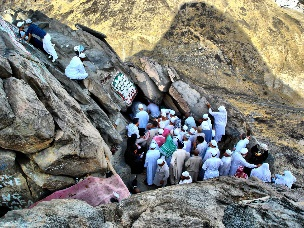
\includegraphics[width=1.34722in,height=1.01046in]{Images/image051.jpg}

\end{marginfigure}


Disons d'emblée que la révélation coranique a commencé près de La
Mecque, dans la grotte de Ḥirā'. Le Coran lui a continué à lui être
révélé jusqu'à sa mort. Pour connaître si un verset est mecquois ou
médinois, on va s'appuyer sur les compagnons~: \emph{un tel a entendu
que Muḥammad, alors qu'il été à La Mecque, a récité le verset\ldots{}
etc.}

Pour autant, il n'y a pas toujours consensus parmi les compagnons, et
par suite, parmi les savants, pour savoir ce qui relève de La Mecque ou
de Médine. Ces divergences ne portent pas tant sur les sourates que sur
des versets de ces sourates. Une sourate en effet, peut contenir des
versets mecquois et des versets médinois.

\begin{Synthesis}
{l'islam, comme système religieux, est achevé.
l'iǧtihād~n'a pas été aboli et il est resté intégré à la réflexion
savante. En revanche, le taqlīd~que les~réformateurs ont remis en
cause.}
\end{Synthesis}

On trouve dans la plupart des ouvrages de \emph{`ulūm al-qur'ān} (le mot
est traduit dans le titre, je dis ça au cas où\ldots) une liste des
sourates mecquoises et médinoises\sn{Par exemple, Zarkašī,
  \emph{al-Burhān fī `ulūm al-Qur'ān}, Cairo, 1958, Vol.1, p. 193.}. Ces
listes sont aussi accompagnées d'un ordre chronologique des sourates.
Mais il faut savoir que cet ordre est sujet à discussion puisque selon
les auteurs, il peut différer. Cela n'est pas sans conséquence\ldots{}

Pour déterminer l'origine d'un verset, il faut donc procéder à
l'\emph{iǧtihād}. Dans cet esprit, on va distinguer des caractéristiques
spécifiques à chaque époque~: thématique, expressions, etc.


\subsection{{Caractéristiques des versets
mecquois
}}


\paragraph{Appel à la conversion}

La prédication mecquoise se caractérise par un appel à la conversion. Il
y a quelque chose de Jean-Baptiste qui appelle à se convertir. Il s'agit
d'abandonner les idoles, les faux dieux et de se tourner vers le Dieu
unique Allāh.


\paragraph{Dimension eschatologique}

Ces versets ont aussi une dimension eschatologique~qui tend à rendre
plus urgente la conversion~: la fin des temps est proche.


\paragraph{Vie droite}

Il s'ensuit un appel à mener une vie droite et juste conformément au
chemin tracé par Dieu (Allāh).


\subsection{{  les thématiques des versets
médinois
} }

 
\paragraph{Abraham}\label{abraham}

le thème d'Abraham comme «~Père des croyants~» où Abraham est dit
d'une part \emph{ḥanīf}, c'est-à-dire monothéiste exclusif, mais aussi
\emph{muslim}, c'est-à-dire soumis, abandonné à Dieu, et ni juif ni
chrétien, date de la période médinoise.

\begin{longtable}{p{5cm}p{5cm}}
\toprule
\endhead
«~Abraham n'était ni juif ni chrétien, mais il était un monothéiste
exclusif, abandonné à Dieu~; il n'était pas au nombre des polythéistes.
Les hommes les plus proches d'Abraham sont vraiment ceux qui l'ont
suivi, ainsi que ce Prophète et ceux qui ont cru~». (S. 3, 67-68). &
\TArabe{مَا كَانَ إِبْرَاهِيمُ يَهُودِيًّا وَلَا نَصْرَانِيًّا وَلَكِنْ
كَانَ حَنِيفًا مُسْلِمًا وَمَا كَانَ مِنَ الْمُشْرِكِينَ إِنَّ أَوْلَى
النَّاسِ بِإِبْرَاهِيمَ لَلَّذِينَ اتَّبَعُوهُ وَهَذَا النَّبِيُّ
وَالَّذِينَ آَمَنُوا وَاللَّهُ وَلِيُّ الْمُؤْمِنِينَ} \\
\bottomrule
\end{longtable}

Ce verset a bien sûr donné lieu à de multiples commentaires. Il est
souvent interprété dans le sens où Abraham est dépositaire de la
religion originelle avant son altération par les juifs et les chrétiens.
Souvent ne veut pas pour autant dire toujours. Il y a d'autres
lectures\ldots{}

Sur la \emph{ḥanīfiyya}, c'est-à-dire cette affirmation d'une foi
exclusive, sans associationnisme (\emph{širk}), le Coran raconte un
dialogue entre Dieu et Abraham\emph{~}:

\begin{quote}
    «~Ainsi avons-Nous montré à Abraham le royaume des cieux et de la terre
afin qu'il soit de ceux qui croient avec conviction. Lorsque la nuit
l'enveloppa, il vit une étoile et dit : « Voilà mon Seigneur ! » Puis,
lorsqu'elle disparut, il dit : « Je n'aime pas les choses qui
disparaissent~». Il vit ensuite la lune se lever et dit : « Voilà mon
Seigneur ! » Puis, lorsqu'elle disparut, il dit : « Si mon Seigneur ne
me guide pas, je serai assurément du nombre des égarés. » Voyant enfin
le soleil levant, il dit : « Voilà mon Seigneur ! Celui-ci est plus
grand~». Puis, lorsqu'il disparut, il dit : « Ô mon peuple, je désavoue
tout ce que vous associez à Dieu. Je tourne mon visage comme un vrai
croyant vers Celui qui a créé les cieux et la terre, et je ne suis pas
de ceux qui Lui donnent des associés » (S. 6, 76-79)  \TArabe{فَلَمَّا
جَنَّ عَلَيْهِ اللَّيْلُ رَأَى كَوْكَبًا قَالَ هَذَا رَبِّي فَلَمَّا
أَفَلَ قَالَ لَا أُحِبُّ الْآَفِلِينَ (}76\TArabe{) فَلَمَّا رَأَى الْقَمَرَ
بَازِغًا قَالَ هَذَا رَبِّي فَلَمَّا أَفَلَ قَالَ لَئِنْ لَمْ يَهْدِنِي
رَبِّي لَأَكُونَنَّ مِنَ الْقَوْمِ الضَّالِّينَ (}77\TArabe{) فَلَمَّا رَأَى
الشَّمْسَ بَازِغَةً قَالَ هَذَا رَبِّي هَذَا أَكْبَرُ فَلَمَّا أَفَلَتْ
قَالَ يَا قَوْمِ إِنِّي بَرِيءٌ مِمَّا تُشْرِكُونَ (}78\TArabe{) إِنِّي
وَجَّهْتُ وَجْهِيَ لِلَّذِي فَطَرَ السَّمَاوَاتِ وَالْأَرْضَ حَنِيفًا
وَمَا أَنَا مِنَ الْمُشْرِكِينَ (}79\TArabe{) وَحَاجَّهُ قَوْمُهُ قَالَ
أَتُحَاجُّونِّي فِي اللَّهِ وَقَدْ هَدَانِ وَلَا أَخَافُ مَا تُشْرِكُونَ
بِهِ إِلَّا أَنْ يَشَاءَ رَبِّي شَيْئًا وَسِعَ رَبِّي كُلَّ شَيْءٍ
عِلْمًا أَفَلَا ت

َتَذَكَّرُونَ} \\

\end{quote}
Ce dialogue est connu dans le monde biblique. Il se retrouve dans des
écrits juifs, chrétiens et judéo-chrétiens~: Ainsi par exemple, dans
\emph{L'Apocalypse d'Abraham}\sn{~\emph{L'Apocalypse d'Abraham}
  est un livre apocryphe dont on dispose de manuscrits en roumain et en
  slave. L'original devait être une traduction grecque de l'hébreu ou de
  l'araméen. Le texte est daté du premier siècle, sans doute après la
  destruction du Temple de Jérusalem par les Romains en 70. Apocalypse
  d'Abraham car il est question de la vie du patriarche et de son
  dialogue avec Dieu mais aussi d'une ascension et de visions où les
  anges* jouent un rôle important, notamment celle du char céleste de
  Dieu (cf. Ez 1).} : «~Plus que la terre, j'appellerai digne de
vénération le soleil car il éclaire de ses rayons le monde et les
différentes atmosphères. Mais celui-là non plus je ne le placerai pas
parmi les dieux, car la nuit, sa course est assombrie par les nuées~»
(7, 1, 7).

Le terme \emph{ḥanīf} est employé par deux fois pour Muḥammad (S. 10,
105 et 30, 30), Muḥammad étant lui-même chargé de détruire les idoles de
la Ka`ba.

L'injonction est aussi adressée aux Gens du Livre à qui il fut demandé
seulement d'agir «~comme des \emph{ḥunafā'} (\emph{ḥunafā' est le
pluriel de ḥanīf}) et non comme des polythéistes~» (S. 22, 31).


\paragraph{Falsification des
écritures}

- toute la théologie coranique relative à la falsification des
écritures~:
\begin{quote}
«~Comment pouvez-vous désirer qu'ils croient avec vous, alors que
certains d'entre eux ont falsifié sciemment~la Parole de Dieu, après
l'avoir entendue~?» (S. 2, 75) est de Médine. \TArabe{أَفَتَطْمَعُونَ أَنْ
يُؤْمِنُوا لَكُمْ وَقَدْ كَانَ فَرِيقٌ مِنْهُمْ يَسْمَعُونَ كَلَامَ
اللَّهِ ثُمَّ يُحَرِّفُونَهُ مِنْ بَعْدِ مَا عَقَلُوهُ وَهُمْ
يَعْلَمُون} \\
\end{quote}


\paragraph{Vie à Médine}

- De même, les prescriptions relatives à la manière de vivre datent de
Médine~:

\begin{longtable}{p{5cm}p{5cm}}
\toprule
\endhead
«~Il n'appartient pas à un croyant ou une croyante, une fois qu'Allah ou
Son messager ont décidé une chose d'avoir encore le choix dans leur
façon d'agir. Et quiconque désobéit à Allah et son messager s'est égaré
certes, d'un égarement évident~» (S. 33, 36).
&
\TArabe{وَمَا كَانَ
لِمُؤْمِنٍ وَلَا مُؤْمِنَةٍ إِذَا قَضَى اللَّهُ وَرَسُولُهُ أَمْرًا أَنْ
يَكُونَ لَهُمُ الْخِيَرَةُ مِنْ أَمْرِهِمْ وَمَنْ يَعْصِ اللَّهَ
وَرَسُولَهُ فَقَدْ ضَلَّ ضَلَالًا مُبِينًا} \\
\bottomrule
\end{longtable}

Toutes les questions relatives au statut social et légal sur le mariage,
le divorce, les héritages, les punitions\ldots{} sont aussi de Médine.

Outre les différences thématiques, on trouve différentes
expressions~propres à chaque période. Ainsi, les adresses \textbf{«~Ô
vous qui croyez~» ou «~Ô gens du Livre~» caractérisent les sourates
médinoises} tandis que \textbf{«~Ô vous les gens~» est plutôt
mecquoise}.


\subsection{Importance de la
chronologie}

Dans la mesure où le Coran ne suit pas l'ordre chronologique, en quoi
est-il si important du point de vue des sciences coraniques de connaître
cette chronologie et la nature de la sourate (mecquoise ou médinoise)~?

Il s'avère que cette connaissance a des conséquences décisives dans la
référence des versets selon les situations posées. On se souviendra que
les versets mecquois «~parlent~» tout particulièrement aux musulmans
vivant dans une situation difficile et d'hostilité à leur égard. Au
contraire, dans le cadre d'une société musulmane, on s'appuiera
spécifiquement sur les versets de Médine.

Par ailleurs, la chronologie permet de mieux saisir l'évolution des
positions du Coran sur une même question, l'évolution des pratiques, à
l'instar par exemple de la consommation d'alcool.

Enfin, la chronologie permet de distinguer \textbf{les versets
abrogeants des versets abrogés}, c'est-à-dire en cas de contradiction,
celui qui abroge l'autre. Le critère retenu, comme nous le verrons, est
chronologique~: le dernier verset révélé abroge celui qui le précède.


\section{La question de l'abrogation
}\label{ii.-la-question-de-labrogation}

La question de l'abrogation est essentielle dans l'exégèse coranique.
Tandis que le Coran est compris comme une guidance universelle, la
chronologie du Coran montre l'existence d'une progressivité de la
révélation. Sur ce point, il existe selon les commentateurs une
pédagogie divine.

Pour autant, sa pratique n'est pas sans difficulté. Elle est au cœur des
débats contemporains sur l'exégèse coranique dans la mesure où
l'abrogation s'effectue dans le sens chronologique de la révélation. Or,
il s'ensuit que les versets médinois, c'est-à-dire les plus prescriptifs
et légalistes, abrogent les versets plus universels de La Mecque.
Au-delà même de la question versets médinois / versets mecquois, le
verset «~Pas de contrainte en religion~» (S.2, 256) qui est un verset
médinois, est-il abrogé par les versets dits \emph{de l'épée} (S,9,5),
eux aussi médinois~qui lui sont postérieurs ? C'est ce que soutient par
exemple le savant saoudien Ibn Bāz (1910-1999).

\begin{longtable}{p{5cm}p{5cm}}
\toprule
Nulle contrainte en religion! Car le bon chemin s'est distingué de
l'égarement. Donc, quiconque mécroit au Rebelle tandis qu'il croit en
Allah saisit l'anse la plus solide, qui ne peut se briser. Et Allah est
Audient et Omniscient. (S.2, 256)
&
\TArabe{لَا إِكْرَاهَ فِي الدِّينِ قَد
تَّبَيَّنَ الرُّشْدُ مِنَ الْغَيِّ فَمَن يَكْفُرْ بِالطَّاغُوتِ
وَيُؤْمِن بِاللَّهِ فَقَدِ اسْتَمْسَكَ بِالْعُرْوَةِ الْوُثْقَى لَا
انفِصَامَ لَهَا وَاللَّهُ سَمِيعٌ عَلِيمٌ} \\
\midrule
\endhead
Après que les mois sacrés expirent, tuez les associateurs où que vous
les trouviez (S,9,5),. Capturez-les, assiégez-les et guettez-les dans
toute embuscade. Si ensuite ils se repentent, accomplissent la Salât et
acquittent la Zakât, alors laissez-leur la voie libre, car Allah est
Pardonneur et Miséricordieux.
&
\TArabe{ فَإِذَا انسَلَخَ الْأَشْهُرُ الْحُرُمُ
فَاقْتُلُوا الْمُشْرِكِينَ حَيْثُ وَجَدتُّمُوهُمْ وَخُذُوهُمْ
وَاحْصُرُوهُمْ وَاقْعُدُوا لَهُمْ كُلَّ مَرْصَدٍ فَإِن تَابُوا
وَأَقَامُوا الصَّلَاةَ وَآتَوُا الزَّكَاةَ فَخَلُّوا سَبِيلَهُمْ إِنَّ
اللَّهَ غَفُورٌ رَّحِيمٌ 
} \\
\bottomrule
\end{longtable}

\vide{un-principe-juridique-fonduxe9-sur-le-coran}{%
\subsection{{ Un principe juridique fondé sur le
Coran~?
}}\label{un-principe-juridique-fonduxe9-sur-le-coran}}

On distingue donc entre verset abrogé (\emph{ayāh mansūḫa}) et verset
abrogeant (\emph{ayāh nāsiḫa}). Ce principe repose sur le verset
coranique suivant~:

\begin{longtable}{p{5cm}p{5cm}}
\toprule
\endhead
«~nous n'abrogeons aucun verset. Nous n'en faisons oublier aucun sans le
remplacer par un autre qui soit meilleur ou équivalent~» (S. 2, 106). 
&
\TArabe{مَا نَنْسَخْ مِنْ آَيَةٍ أَوْ نُنْسِهَا نَأْتِ بِخَيْرٍ مِنْهَا أَوْ
مِثْلِهَا} \\
\bottomrule
\end{longtable}

Cependant, l'analyse littéraire a montré que le contexte de ce verset ne
renvoie pas au Coran mais aux Écritures antérieures\sn{Michel
  \textsc{Cuypers}, «~Le verset de l'abrogation (2, 106) dans son
  contexte rhétorique~» dans Mehdi Azaiez (dir.) avec la collaboration
  de Sabrina \textsc{Mervin}, \emph{Le Coran : nouvelles approches},
  Paris, CNRS, 2013.}. \textbf{Dieu n'abroge pas les versets de la Torah
sans les remplacer par d'autres~: les versets coraniques}. Autrement
dit, on ne trouverait pas dans le Coran une justification de
l'abrogation du Coran par le Coran. Certains théologiens l'ont aussi
noté, à l'exemple du fondamentaliste Mawdudi (1903-1979)\sn{\textsc{Mawdudi},
  \emph{Comprendre le Coran}.}. On a le même problème avec la théologie
protestante et le principe fondamental de la \emph{sola scriptura}. Mais
où l'Écriture dit-elle que pour une question théologique, on ne peut
recourir pour répondre qu'à l'Écriture~?

Cette question n'est pas anecdotique et peut avoir de grandes
répercussions dans la refondation de la pensée musulmane à laquelle
appellent bien des penseurs musulmans.

\vide{un-enjeu-thuxe9ologique-dieu-peut-il-se-contredire}{%
\subsection{{Un enjeu théologique~: Dieu peut-il se
contredire~?
}}\label{un-enjeu-thuxe9ologique-dieu-peut-il-se-contredire}}

Le fait que des versets coraniques ne tiennent pas la même position
ouvre à une difficulté majeure : Comment la Parole de Dieu, immuable,
éternelle, peut-elle contenir des versets contradictoires~? Dieu ne
pouvant être versatile, comment sa Parole pourrait-elle l'être ? N'y
a-t-il pas le risque d'affaiblir et de remettre en cause l'affirmation
de la nature parfaite du Coran~?

Pour les mu`tazilites, c'est-à-dire les rationalistes, le problème ne se
pose pas~car la Loi donnée par Dieu suit l'intérêt (\emph{al-maṣlaha}).
Chaque contexte est singulier et Dieu donne un commandement qui guide la
communauté dans le sens qui lui est le plus profitable. Ce principe
exégétique a influencé la jurisprudence islamique~: au
11\textsuperscript{ème} siècle, le légiste al-Māwardī (974-1058) écrit~:

«~L'intérêt diffère selon les époques~: un statut shariatique peut très
bien avoir été dans le sens de son intérêt à une époque et un autre,
abrogeant le précédent, aller dans son sens à une autre époque. Chacun
des deux statuts présente un intérêt en son temps, même s'ils sont
antinomiques~»\sn{~Eric \textsc{Chaumont}, «~Abrogation~», dans
  Amir \textsc{Moezzi}, \emph{Dictionnaire du Coran}, \emph{op. cit}.,
  p. 14.}.

Une conséquence est d'introduire dans la Loi divine une distance
critique et un principe de relativisme. La communauté n'applique donc
pas une Loi dans sa littéralité, mais doit d'abord se poser la question
de l'intérêt pour elle-même, dans un contexte géographique et politique
propre. Vous voyez que bien sûr, les fondamentalistes y voient un risque
d'instrumentaliser la Loi divine et de lui ôter son caractère sacré. Ils
accusent les rationalistes et avec eux les nouveaux penseurs de ne
prendre dans la Loi que ce qui les arrange\ldots{} D'autres, plus
contempteurs, diront avec méfiance qu'une lecture souple de la loi ne
peut être que temporaire et s'inscrire dans une stratégie progressive
d'islamisation\ldots{} C'est compliqué, mais il faut connaître toutes
ces discussions et subtilités en arrière-fond de la question de
l'abrogation. Nous y reviendrons quand nous aborderons le droit
islamique (\emph{fiqh}).


\paragraph{l'acharisme}{{ L'acharisme~est une
école~{théologique}~de
l'{islam}, fondée
par~{Abu
Al-Hasan
al-ʾAshʿarī}~({873}-{935}).
(\TArabe{الأشعرية}~). Cette école de pensée se répandit très vite et devint
l'école théologique majoritaire. D'abord adepte du~mu'tazilisme~il~s'en
sépara au moins sur deux points
essentiels~:} 
\begin{itemize}
    \item il affirme que l'homme est libre de ses actions mais
c'est Dieu qui crée ses actes (bons ou
mauvais)
\item Il déclare que le~Coran~est incréé car, étant la Parole de Dieu lui-même, elle fait donc partie de lui
\end{itemize}}


Pour le courant théologique \textbf{asharite}, une telle thèse est
impossible : \textbf{Dieu ne peut être versatile dans sa volonté}.
\textbf{Al-Rāzī} (m. 1209), le grand commentateur du Coran, répond en
soulignant la \textbf{dimension pédagogique de Dieu}~: Dieu ne se
contredit pas mais prend l'homme tel qu'il est et le fait avancer à son
rythme.
\mn{Al-razi, théologien musulman de rite chaféite, est né à
Ray ou 1150, et mort en 1210 à Hérat. Musulman d'obédience sunnite, il
écrit le Le Grand Commentaire du Coran (aussi connu sous le titre Les
Clés de l'invisible). fervent défenseur de la doctrine de
l'unicité}

\vide{abrogation-et-falsification}{%
\subsection{Abrogation et
falsification}\label{abrogation-et-falsification}}

L'abrogation concerne aussi et surtout les écritures antérieures. Pour
les musulmans, les livres donnés aux Juifs et chrétiens ont été altérés,
falsifiés (\emph{taḥrīf}, S. 5, 13) et Dieu leur a substitué l'Écriture
authentique. C'est le \emph{tabdīl} (S. 7, 162) qui consiste donc à
\textbf{remplacer l'erreur par la vérité.}

La dénonciation de la falsification des Écritures prend trois formes. Le
Coran accuse les gens du Livre de ne pas tout dire, d'avoir fabriqué de
faux versets, ou encore d'en avoir effacé certains.

\begin{itemize}
\item
  Ne pas tout dire~: «~Ô Détenteurs de l'Écriture~! Pourquoi
  travestissez-vous la Vérité au moyen du faux~? Pourquoi tenez-vous
  secrète la Vérité, alors que vous savez~? (3, 71).
\end{itemize}

\TArabe{يَا أَهْلَ الْكِتَابِ لِمَ تَلْبِسُونَ الْحَقَّ بِالْبَاطِلِ
وَتَكْتُمُونَ الْحَقَّ وَأَنْتُمْ تَعْلَمُونَ}

\begin{itemize}
\item
  Avoir fabriqué un faux~: «~malheur à ceux qui de leurs propres mains
  composent un livre, puis le présentent comme venant d'Allah pour en
  tirer un vil profit~! Malheur à eux à cause de ce qu'ils en
  profitent~» (S. 2, 79). On retrouve ici le cœur de la polémique
  anti-chrétienne où l'Évangile aurait été dénaturé.
\end{itemize}

\TArabe{فَوَيْلٌ لِلَّذِينَ يَكْتُبُونَ الْكِتَابَ بِأَيْدِيهِمْ ثُمَّ
يَقُولُونَ هَذَا مِنْ عِنْدِ اللَّهِ لِيَشْتَرُوا بِهِ ثَمَنًا قَلِيلًا
فَوَيْلٌ لَهُمْ مِمَّا كَتَبَتْ أَيْدِيهِمْ وَوَيْلٌ لَهُمْ مِمَّا
يَكْسِبُونَ}

\begin{itemize}
\item
  Avoir effacé~: «~Ô détenteurs de l'Écriture~! notre messager est venu
  à vous, vous exposant une grande partie de l'Écriture que vous cachiez
  et aviez effacée aussi une grande partie de celle-ci~» (S. 5, 15).
\end{itemize}

\TArabe{يَا أَهْلَ الْكِتَابِ قَدْ جَاءَكُمْ رَسُولُنَا يُبَيِّنُ لَكُمْ
كَثِيرًا مِمَّا كُنْتُمْ تُخْفُونَ مِنَ الْكِتَابِ وَيَعْفُو عَنْ
كَثِيرٍ قَدْ جَاءَكُمْ مِنَ اللَّهِ نُورٌ وَكِتَابٌ مُبِينٌ}

L'argument théologique de la falsification des écritures n'est pas
nouveau. Il a déjà été utilisé par des chrétiens à l'encontre des juifs.
Mani, le philosophe prophète du deuxième siècle, y a eu aussi recours.

\vide{quels-sont-les-versets-abrogeants-et-abroguxe9s}{%
\subsection{{Quels sont les versets abrogeants~et
abrogés ?
}{ Quels sont les versets abrogeants~et abrogés ? }}\label{quels-sont-les-versets-abrogeants-et-abroguxe9s}}

Là encore, les spécialistes en \emph{`ulūm al-qur'ān}  dressent la
liste des versets abrogés ou abrogeants. Elles ne sont pas identiques.

\mn{{Abū l-Fadl al-Suyūtī, né
en~{1445}~au Caire, est un
savant égyptien connu pour son œuvre abondante. Il fut un éminent
savant~Shâfi'ite, un théologien~Ash'arite~de renom. il serait né dans la
bibliothèque familiale ce qui lui valut son surnom de «~fils des
livres~» (ibn al-kutub). D'une mémoire prodigieuse, il connaissait par
cœur quelque deux cent mille hadiths. Il se rattacha à la~ṭarīqa
shādhiliyya~et prôna l'équilibre entre la Loi et la Voie. On lui
reprocha notamment son emploi de l'ijtihād~mais sans qu'il fut jugé
condamnable. D'une façon générale, il rejeta le pouvoir des Mamelouks.
Il prôna la complémentarité de l'exotérisme et
du~ {soufisme}. On lui
attribue jusqu'à 981
ouvrages.}}

Al-Suyūtī (1445-1505) dans son \emph{Itqān} (cet ouvrage est étudié par
tous les musulmans qui font des sciences islamiques pour devenir imam)
note qu'il existe 21 passages coraniques qui ont été abrogés et il
précise que tous ceux qui en désignent d'autres sont dans l'erreur. Cet
ouvrage n'est pas encore traduit en français, mais le Père Michel
Lagarde, père blanc qui a enseigné au PISAI, en prépare la traduction.
Elle vient de paraître en novembre 2017, mais je ne l'ai pas encore pu
consulter. Je vous signale que pour al-Suyūtī, le verset «~Pas de
contrainte en religion~» (S.2, 256) n'est pas abrogé.

On trouve aussi des listes plus restreintes. Shah Waliullah (fameux
musulman indien mort en 1759) ne retient à partir de la liste de
al-Suyūtī que 5 versets~:

\begin{quote}
Abrogé 2, 180, abrogeant~: 4, 11, 12
\end{quote}

\begin{longtable}{p{4cm}p{8cm}}

\toprule
Abrogé 2, 180 & abrogeant~ 4, 11, 12\\
\midrule
\endhead
On vous a prescrit, quand la mort est proche de l'un de vous et s'il
laisse des biens, de faire un testament en règle en faveur de ses père
et mère et de ses plus proches. C'est un devoir pour les pieux. & Voici
ce qu'Allah vous enjoint au sujet de vos enfants: au fils, une part
équivalente à celle de deux filles. S'il n'y a que des filles, même plus
de deux, à elles alors deux tiers de ce que le défunt laisse. Et s'il
n'y en a qu'une, à elle alors la moitié. Quant aux père et mère du
défunt, à chacun d'eux le sixième de ce qu'il laisse, s'il a un enfant.
S'il n'a pas d'enfant et que ses père et mère héritent de lui, à sa mère
alors le tiers. Mais s'il a des frères, à la mère alors le sixième,
après exécution du testament qu'il aurait fait ou paiement d'une dette.
De vos ascendants ou descendants, vous ne savez pas qui est plus près de
vous en utilité. Ceci est un ordre obligatoire de la part d'Allah, car
Allah est, certes, Omniscient et Sage.

Et à vous la moitié de ce que laissent vos épouses, si elles n'ont pas
d'enfants. Si elles ont un enfant, alors à vous le quart de ce qu'elles
laissent, après exécution du testament qu'elles auraient fait ou
paiement d'une dette. Et à elles un quart de ce que vous laissez, si
vous n'avez pas d'enfant. Mais si vous avez un enfant, à elles alors le
huitième de ce que vous laissez après exécution du testament que vous
auriez fait ou paiement d'une dette. Et si un homme, ou une femme meurt
sans héritier direct, cependant qu'il laisse un frère ou une sœur, à
chacun de ceux-ci alors, un sixième. S'ils sont plus de deux, tous alors
participeront au tiers, après exécution du testament ou paiement d'une
dette, sans préjudice à quiconque. (Telle est l') Injonction d'Allah! Et
Allah est Omniscient et Indulgent. \\
\bottomrule
\end{longtable}

\begin{quote}
Abrogé 2, 240, abrogeant~: 2, 234

Abrogé 8, 65~; abrogeant~: 8, 62

Abrogé 30, 50, abrogeant~: 33, 52

Abrogé 58, 12, abrogeant~: 58, 13.
\end{quote}


\subsection{ L'approche originale de Mahmud Muhammad Taha et \emph{Le
second message de l'islam}}
\mn{Mahmoud Mohammed \textsc{Taha}, \emph{Un islam à
  vocation libératrice}, traduit par Mohamed El Baroudi-Haddaoui et
  Caroline Pailhe, Avant-propos de François Houtart, Préface de Samir
  Amin, Paris, L'Harmattan, 2002, 182 pages.}

Maḥmūd Muḥammad Ṭāha est un libre penseur soudanais, fondateur d'un
mouvement politico-religieux «~al-Iḫwān al-Ğumhūriyyūn~» (les frères
Républicains). Ṭāha est né en 1909 à Rufâ`a et il a fondé en 1945 le
parti al\emph{-Ḥizb al-Ğumhūrī} en vue de fonder une République fédérale
indépendante du Soudan. C'est un homme spirituel et au cours d'une de
ses méditations, il reçut une illumination, dans laquelle il lui était
enseigné que le Coran contient deux messages~: celui de Médine
(\emph{šarī`a}) et celui de La Mecque (principes de base spirituels, les
\emph{uṣūl} de la religion islamique). Le premier message~a une vocation
limitée dans le temps, tandis que le second message a une portée
universelle. En appliquant le principe de l'abrogation en lien avec
cette «~révélation~» il propose une exégèse dans laquelle seuls les
versets universels mecquois doivent être portés par la prédication
musulmane.

Sa théorie novatrice dérangea~; il fut accusé et combattu par les
musulmans orthodoxes et les frères musulmans soudanais (\emph{Iḫwān
al-Muslimūn}). Accusé d'apostasie~en 1968 puis en 1985, il est
finalement exécuté en janvier 1985\sn{Annette \textsc{Oevermann},
  «~Ma\underline{h}mûd Mu\underline{h}ammad \underline{T}âha~»,
  \emph{Encyclopédie de l'islam}, p. 105.~}

\begin{quote}
     «~Pour résumer la pensée riche, audacieuse et subtile des
  `Républicains', on peut dire sans trop la caricaturer que le
  \emph{Second message} s'adresse à l'individu pour affirmer et œuvrer à
  réaliser sa `liberté absolue', au point d'être `un Dieu en devenir'~;
  et aux sociétés humaines afin d'instaurer un système où `socialisme'
  et `démocratie' seront enfin réconciliés, et où règnera une égalité.
  absolue entre les hommes, les sexes et les races~» cité par Mustapha Khayati
  \sn{\textsc{ Mustapha Khayati}, ``Le pensée de Mahmud Muhammad Taha'', in Hervé
  \textsc{Bleuchot}, Christian \textsc{Delmet}, Derek \textsc{Hopwood}
  (ed.), \emph{Sûdân}, History, identity, ideology, IRENAM, Oxford,
  1991, p. 290.}
\end{quote}
 

Le message de Ṭāha n'a pas pu être entendu en raison de trois grandes
difficultés~:
\begin{itemize}
    \item son exégèse prend à rebours la tradition qui consistait à abroger
l'ancien par le nouveau.
\item sa lecture a un ancrage mystique, personnel et manque d'assises
exégétiques, méthodologiques et épistémologiques.
\item la portée politique de son message.
\end{itemize}


Aujourd'hui, le défi est de repenser l'abrogation mais au sein même des
données de la tradition. Il faut revenir à l'étymologie, au sens que les
mots avaient pour les compagnons, aux avis des premiers
commentateurs\ldots{} pour cela, il faut aussi recourir aux données des
sciences humaines et des avancées dans notre connaissance du Coran et de
ses commentaires.

%---------------------------------------------------------------------------------------

 
 



 

\vide{iii.-lexuxe9guxe8se-coranique}{%
\section{{L'exégèse coranique
}}\label{iii.-lexuxe9guxe8se-coranique}}

\paragraph{Introduction}
\begin{quote}
    {« Le courant littéraliste, qui considère que le Coran se suffit à
lui-même, que ses ambiguïtés sont voulues par Dieu et que l'interpréter
est source d'égarements, a toujours existé, mais il a longtemps été très
marginal en islam »,}
\end{quote}
~rappelle l'historien Mohammad
Ali Amir-Moezzi 
 . C'est depuis une cinquantaine d'années, avec
l'essor du salafisme, que cette conception a gagné du terrain,
valorisant essentiellement l'apprentissage par cœur.
Plusieurs anecdotes transmises par la tradition islamique montrent un
croyant venant consulter le prophète Mohammed sur le sens de tel ou tel
verset. Il faut dire que le texte coranique est un corpus
particulièrement ardu, au contenu souvent allusif, parfois
contradictoire. Non content d'entremêler des thèmes et registres
différents, il n'a pas été agencé selon l'ordre chronologique de la
révélation.

 
D'où la nécessité de l'interpréter. Riche de plusieurs milliers de
volumes, le commentaire du Coran a connu son âge d'or du
VIII\textsuperscript{e}~au XII\textsuperscript{e}~siècle.\emph{~« Les
grands courants de pensée islamiques se sont tous développés à partir de
la même interrogation : comment comprendre l'écriture sainte
?,~}explique Mohammad Ali Amir-Moezzi.\emph{~­L'islam a hérité de cette
culture exégétique des milieux bibliques au sein desquels il s'est
développé. »}

Les commentateurs ne pouvaient toutefois pas interpréter le Coran à leur
guise. On dénombre trois méthodes principales : 
\bi 
\item la traditionnelle avait
essentiellement recours aux sources scripturaires (le Coran et les
hadiths) et à des analyses sur la langue arabe et la culture tribale ;
\item la rationnelle faisait appel à la logique et à la pensée spéculative, la
logique aristotélicienne ; 
\item et la mystique reposait sur une~\emph{«
illumination »}.
\ei

\subsection{ L'exégèse sunnite~}


\subsubsection{{Terminologie~: \emph{tafsīr} et
\emph{ta'wīl}}}

Je vous avais annoncé une terminologie un peu technique. Ce n'était pas
une promesse de Gascon. Accrochez-vous.

\begin{Def}[tafsīr]
Le \emph{tafsīr} désigne avant tout le commentaire littéral et intégral
du texte coranique sur la base du Coran lui-même, selon le principe
qu'au Coran seul appartient le monopole d'interprétation, et des
matériaux transmis par le prophète Muḥammad ou ses compagnons
(\emph{hadîths}).
\end{Def}

\begin{Def}[ta'wīl, Muhkam, Mutashabih]
Le \emph{ta'wīl} porte en revanche sur l'interprétation du texte en se
fondant sur l'existence de versets obvies (\textit{Muhkam}) et de versets abscons (\textit{Mutashabih}) tels
qu'énoncés dans la Sourate 3, 7~.
\end{Def}


\begin{quote}
«~C'est lui {[}Dieu{]} qui a fait descendre sur toi le Livre. On y
trouve \textbf{des versets clairs} -- la Mère du Livre -- et d'autres
obscurs. Ceux dont les cœurs penchent vers l'erreur s'attachent à ce qui
est obscur car ils recherchent la discorde et ils sont avides
d'interprétations~; mais nul autre que Dieu ne connaît l'interprétation
du Livre. Ceux qui sont enracinés dans la Science disent~: `\,`Nous y
croyons~! Tout vient de notre Seigneur~!'\,' Mais seuls, les hommes
doués d'intelligence s'en souviennent~». Sourate 3, 7


\TArabe{هُوَ الَّذِي أَنْزَلَ عَلَيْكَ الْكِتَابَ مِنْهُ آَيَاتٌ مُحْكَمَاتٌ
هُنَّ أُمُّ الْكِتَابِ وَأُخَرُ مُتَشَابِهَاتٌ فَأَمَّا الَّذِينَ فِي
قُلُوبِهِمْ زَيْغٌ فَيَتَّبِعُونَ مَا تَشَابَهَ مِنْهُ ابْتِغَاءَ
الْفِتْنَةِ وَابْتِغَاءَ تَأْوِيلِهِ وَمَا يَعْلَمُ تَأْوِيلَهُ إِلَّا
اللَّهُ وَالرَّاسِخُونَ فِي الْعِلْمِ يَقُولُونَ آَمَنَّا بِهِ كُلٌّ
مِنْ عِنْدِ رَبِّنَا وَمَا يَذَّكَّرُ إِلَّا أُولُو الْأَلْبَابِ}

"He it is Who has revealed the Book to you; some of its verses are
decisive (Muhkam), they are the basis of the Book, and others are
allegorical (Mutashabih); then as for those in whose hearts there is
perversity they follow the part of it which is allegorical, seeking to
mislead and seeking to give it (their own) interpretation. but none
knows its interpretation except Allah, and those who are firmly rooted
in knowledge say: We believe in it, it is all from our Lord; and none do
mind except those having understanding."
\end{quote}
\vide{les-versets-clairs-et-les-versets-obscurs}{%
\subsubsection{{Les versets clairs et les versets
obscurs
} }\label{les-versets-clairs-et-les-versets-obscurs}}

Si le Coran insiste à maintes reprises sur la clarté et la limpidité de
son expression, ce verset apporte une nuance importante.

Pour Ibn Mas`ūd~: la distinction entre \emph{muḥkam} et \emph{mutašābih}
est la même qu'entre abrogeant et abrogé, ni plus ni moins.

Mais pour Muǧāhid (104/722), cette distinction renvoie à des catégories
éthiques~pour lesquelles Dieu a prescrit sans confusion ce qui est
licite (\emph{ḥalāl}) ou interdit (\emph{ḥarām}).

Pour al-Šāfi`ī (204/820)~: est \emph{muḥkam} ce qui ne peut
s'interpréter que d'une seule manière tandis que \emph{mutašābih}
renvoie à la possibilité d'interprétations plurielles.

Toutefois, la signification du \emph{muḥkami}, c'est-à-dire des versets
clairs n'est accessible qu'aux savants~; tandis que le sens des versets
obscurs est réservé exclusivement à Dieu.

Les exégètes vont ainsi identifier les versets du Coran selon leur degré
d'équivocité. Un texte (\emph{naṣṣ} pl. \emph{nuṣūṣ})~dont la
compréhension est évidente est qualifié de \emph{mufassar}, de
\emph{mubayyan} ou de \emph{mufaṣṣal.} En revanche, si son sens n'est
pas intelligible à son seul énoncé il est dit \emph{muğmal}.

Mais encore~? Retenez de tout cela que dans une discussion théologique,
il ne suffit pas de citer un verset, il faut aussi s'assurer que son
sens est maîtrisé par celui qui le cite et qu'il en connaît la catégorie
d'évidence.

\vide{les-circonstances-de-la-ruxe9vuxe9lation-asbux101b-al-nuzux16bl}{%
\subsection{{Les circonstances de la révélation
(\emph{asbāb al-nuzūl})
}}\label{les-circonstances-de-la-ruxe9vuxe9lation-asbux101b-al-nuzux16bl}}
\begin{Def}[asbāb al-nuzūl]
Les \emph{asbāb al-nuzūl} d'un verset sont définies comme «une
situation, un évènement particulier ou une question posée à Muḥammad à
la suite desquels une révélation survint en guise de réponse divine».
\end{Def}


La connaissance de ces circonstances est nécessaire à la compréhension
des versets coraniques. Or, ces circonstances sont connues par les
témoignages des compagnons de Muḥammad lesquels se retrouvent dans la
\emph{Sīra}. Ici, il apparaît clairement l'existence d'un enchevêtrement
intertextuel entre la \emph{Sīra} et les propos du Prophète, d'une part,
et le Coran d'autre part, dans la mesure où les circonstances
contribuent à la compréhension du Coran.

Ceci toutefois n'est pas sans difficulté dans la mesure où les
compilations de \emph{ḥadīṯ} ou la mise en forme de la \emph{Sīra} sont
postérieures au Coran\ldots{} Il s'ensuit que les circonstances de la
révélation ont conduit souvent à enfermer le sens du texte coranique.
Aujourd'hui, les nouveaux penseurs de l'islam en appellent à sortir le
Coran du \emph{tafsīr} parce qu'ils y voient une sédimentation de son
sens.

Tous les versets du Coran n'ont pas nécessairement de circonstances. Au
sein d'une même sourate, certains versets peuvent être munis de
circonstances et d'autres non.

Exemple de la sourate 96, al-`Alaq, l'adhérence
\begin{quote}
   1. Lis, au nom de ton Seigneur qui a créé,\\
2. qui a créé l'homme d'une adhérence.\\
3. Lis ! Ton Seigneur est le Très Noble,\\
4. qui a enseigné par la plume {[}le calame{]},\\
5. a enseigné à l'homme ce qu'il ne savait pas.

6. Prenez-garde ! Vraiment l'homme devient rebelle,

7. dès qu'il estime qu'il peut se suffire à lui-même (à cause de sa
richesse). 
\end{quote}


La question des circonstances de la révélation pose aussi une question
théologique~: dans la mesure où le Coran est le Livre éternel écrit de
toute éternité, comment peut-il être ainsi lié à des conditions
historiques, à des évènements particuliers survenus au cours de la vie
de Muḥammad~?

\vide{lexuxe9guxe8se-rationaliste-des-mutazilites}{%
\subsection{{L'exégèse rationaliste des mu`tazilites
}}\label{lexuxe9guxe8se-rationaliste-des-mutazilites}}

Je rappelle que les mu`tazilites sont à l'origine d'un courant de pensée
théologique qui a élaboré une théologie spéculative (\emph{kalām}).
\label{Def:kalam}
\begin{Def}[kalām]
Théologie spéculative
\end{Def}
Pour les mu`tazilites, le coran est forcément clair. Dieu ne peut pas
vouloir révéler aux hommes une parole obscure\ldots{} Or, le Coran
contient des passages abscons. Les mu`tazilites disent alors que la
raison permet de comprendre sa parole. Le Coran peut être lu en toute
clarté.

Certes, il y a des anthropomorphismes, on voit Dieu sur un trône\ldots{}
Il est aussi question de sa colère. Mais il s'agit d'images.

Cette théologie est satisfaisante pour l'esprit, elle risque cependant
d'épuiser le sens de la parole de Dieu.

\vide{lexuxe9guxe8se-mystique}{%
\subsection{L'exégèse mystique}\label{lexuxe9guxe8se-mystique}}

Elle est davantage une méditation sur le Coran. Elle part du principe
affirmé dans le \emph{ḥadīṯ} que: «~chaque verset du Coran a un dos et
un ventre et ce ventre a à son tour un ventre et cela jusqu'à sept
ventres~». 
\begin{Def}[Exégèse mystique, ẓāhir, bāṭin]
Il s'agit donc de passer de la formulation littérale,
visible, immédiate (\emph{ẓāhir})~du verset à sa dimension intérieure,
cachée, invisible (\emph{bāṭin}). 
\end{Def}
L'exégèse mystique ne rejette pas
forcément le sens littéral d'un verset, mais elle ne se limite pas à ce
sens.

Je donne un exemple d'interprétation mystique à propose de l'épisode de
l'immolation du fils d'Abraham \textbf{(S. 37, 99-109)~:}

\begin{quote}
«~{[}Abraham{]} dit~:

`Oui, je vais aller vers mon Seigneur, il me guidera. Mon Seigneur~!
Accorde-moi un fils qui soit juste'. Nous lui avons alors annoncé une
bonne nouvelle~: la naissance d'un garçon, doux de caractère. Lorsqu'il
fut en âge d'accompagner son père, celui-ci dit~: `Ô mon fils~! Je me
suis vu moi-même en songe, et je t'immolais~; qu'en penses-tu~?' Il
dit~: `Ô mon père~! Fais ce qui t'est ordonné. Tu me trouveras patient
si Dieu le veut'. Après que tous deux se furent soumis, et qu'Abraham
eut jeté son fils, le front à terre, nous lui criâmes~; `Ô Abraham~! Tu
as cru en cette vision et tu l'as réalisée~: c'est ainsi que nous
récompensons ceux qui font le bien~: voilà l'épreuve concluante'. Nous
avons racheté son fils par un sacrifice solennel. Nous avons perpétué
son souvenir dans la postérité~: `Paix sur Abraham~!' C'est ainsi que
nous récompensons ceux qui font le bien. Il était au nombre de nos
serviteurs croyants~». \\


\TArabe{وَقَالَ إِنِّي ذَاهِبٌ إِلَى رَبِّي سَيَهْدِينِ (}99\TArabe{) رَبِّ هَبْ
لِي مِنَ الصَّالِحِينَ (}100\TArabe{) فَبَشَّرْنَاهُ بِغُلَامٍ حَلِيمٍ
(}101\TArabe{) فَلَمَّا بَلَغَ مَعَهُ السَّعْيَ قَالَ يَا بُنَيَّ إِنِّي
أَرَى فِي الْمَنَامِ أَنِّي أَذْبَحُكَ فَانْظُرْ مَاذَا تَرَى قَالَ يَا
أَبَتِ افْعَلْ مَا تُؤْمَرُ سَتَجِدُنِي إِنْ شَاءَ اللَّهُ مِنَ
الصَّابِرِينَ (}102\TArabe{) فَلَمَّا أَسْلَمَا وَتَلَّهُ لِلْجَبِينِ
(}103\TArabe{) وَنَادَيْنَاهُ أَنْ يَا إِبْرَاهِيمُ (}104\TArabe{) قَدْ
صَدَّقْتَ الرُّؤْيَا إِنَّا كَذَلِكَ نَجْزِي الْمُحْسِنِينَ (}105\TArabe{)
إِنَّ هَذَا لَهُوَ الْبَلَاءُ الْمُبِينُ (}106\TArabe{) وَفَدَيْنَاهُ
بِذِبْحٍ عَظِيمٍ (}107\TArabe{) وَتَرَكْنَا عَلَيْهِ فِي الْآَخِرِينَ
(}108\TArabe{) سَلَامٌ عَلَى إِبْرَاهِيمَ}
\end{quote}
Dans son commentaire, Qušayrī (m.~465)~note qu'Abraham s'est rapproché
de Dieu et que quand il a eu son fils, les choses se sont assises dans
son cœur. Il s'est mis à trop aimer son fils. L'amour de son fils a
rempli son cœur au point d'embarrasser la présence divine en lui et donc
Dieu l'a mis à l'épreuve.

La réponse de l'enfant, «~Fais ce que tu dois accomplir dans la mesure
où c'est un ordre~» rappelle que le Coran ne dit pas explicitement que
c'est un ordre. L'important est que cela a été vécu comme un ordre pour
passer à l'acte.

L'enfant est heureux de ce sacrifice si c'est un ordre divin. L'un et
l'autre suivent les commandements de Dieu. L'enfant accepte non pour le
père, mais pour Dieu.

Qušayrī (m.1074) se demande alors pourquoi Abraham était prêt à
accomplir un tel geste. Dans son commentaire, il dit que pour celui qui
a goûté à l'amitié divine, il est plus facile de sacrifier son propre
fils que de renoncer à la présence divine. Certains auteurs voient dans
la figure du fils celle du moi. Il s'agit de se sacrifier.

Intervient ensuite l'ange Gabriel~: il est une image de la grâce. Tu es
prêt à mourir, mais la mort que tu as acceptée n'est pas la mort, car le
soufi qui est prêt à renoncer à soi est transfiguré par la présence
divine qui s'accomplit en lui.

 
\mn{{Un des grands connaisseurs de Qušayrī est
Pierre Lory p. \pageref{Theol:PierreLory}. Il a donné une conférence à propos de son commentaire
mystique sur les figures de Moïse et d'Aaron. On pourra la consulter
ci-dessous.
} } 
 

\vide{exemples-dexuxe9guxe8se-de-la-fux101tiha}{%
\section{{ Exemples d'exégèse de la \emph{fātiha}
} }\label{exemples-dexuxe9guxe8se-de-la-fux101tiha}}

\emph{Al-fātiha} est la première sourate du Coran. En français, elle se
nomme l'Ouverture ou l'Ouvrante. Pour certains commentateurs, elle est
la quintessence de tout le message du Livre.

Muḥammad Asad (1900-1992), dans \emph{The Message of the Qur'ān}
(1980)~dit que la tradition l'appelle aussi~«~la mère du Livre~»
(\emph{umm al-kitāb})\sn{Muḥammad Asad, \emph{The Message of the
  Qur`ān}, Gibraltar, 1980, p. 1 cité par Hans Küng, op. cit. p. 107.}.

Elle est la prière par excellence que le musulman accomplit en toutes
circonstances. Elle accompagne le rite de la prière quotidienne (un peu
comme le \emph{Notre Père} pour les chrétiens).

Nous allons présenter une exégèse classique et une exégèse moderne. Mais
avant tout, exposons le texte.

\vide{texte-de-la-fux101tiha}{%
\subsubsection{{ Texte de la fātiha
} { 5.1 Texte de la fātiha }}\label{texte-de-la-fux101tiha}}

\begin{longtable}{p{3cm}p{4cm}p{4cm}}
 
\toprule
\endhead
\TArabe{بِسْمِ اللَّهِ الرَّحْمَنِ الرَّحِيمِ (}1\TArabe{)}

\TArabe{الْحَمْدُ لِلَّهِ رَبِّ الْعَالَمِينَ (}2\TArabe{)}

\TArabe{الرَّحْمَنِ الرَّحِيمِ (}3\TArabe{)}

\TArabe{مَالِكِ يَوْمِ الدِّينِ (}4\TArabe{)}

\TArabe{إِيَّاكَ نَعْبُدُ وَإِيَّاكَ نَسْتَعِينُ (}5\TArabe{)}

\TArabe{اهْدِنَا الصِّرَاطَ الْمُسْتَقِيمَ (}6\TArabe{)}

\TArabe{صِرَاطَ الَّذِينَ أَنْعَمْتَ عَلَيْهِمْ غَيْرِ الْمَغْضُوبِ
عَلَيْهِمْ وَلَا الضَّالِّينَ (}7\TArabe{)} & Bismi Allāhi
Ar-Raĥmāni-r-Raĥīm

(2)~Al-Ĥamdu Lillāhi Rabbi-l-`Ālamīn

(3)~Ar-Raĥmāni-r-Raĥīm

(4) Māliki Yawmi-d-Dīn

(5) 'Īyāka Na`budu Wa 'Īyāka Nasta`īn

(6) Ihdinā-ş-Şirāţa-l-Mustaqīm

(7) Şirāţ-Al-Ladhīna 'An`amta `Alayhim Ghayri-l-Maghđūbi `Alayhim Wa
Lā-đ-Đāllīn

&
Au nom de Dieu, le Tout Miséricordieux, le Très Miséricordieux.

Louange à Dieu, Seigneur de l'univers.

Le Tout Miséricordieux, le Très Miséricordieux.

Maître du Jour du Jugement dernier.

C'est Toi {[}Seul{]} que nous adorons, et c'est Toi {[}Seul{]} dont nous
implorons secours.

Guide-nous dans le droit chemin,

la Voie de ceux que Tu as comblés de faveurs, pas celle de ceux qui ont
encouru Ta colère, ni celle des égarés.
\\
\bottomrule
\end{longtable}


\vide{lexuxe9guxe8se-de-la-fux101tiha-selon-al-razux12b}{%
\subsubsection{{L'exégèse de la \emph{fātiha} selon
al-Razī
}}\label{lexuxe9guxe8se-de-la-fux101tiha-selon-al-razux12b}}

Al-Rāzī est né en 543/1148 à Rayy.

Son Commentaire~principal se nomme \emph{Les clés de l'invisible}.

Il est un commentaire mot par mot, verset par verset. C'est un
commentaire explicatif. Rāzī a donc cherché à percer les secrets
grammaticaux, les secrets de la stylistique. Pourquoi tel mot est
employé et pas tel autre~? Pourquoi à telle place~? Pourquoi une phrase
nominale et pas une phrase verbale~?

Al-Rāzi dresse aussi une théologie de la louange à partir de la fātiha.

En effet, il y a deux manières de louer Dieu~: \emph{al-ḥamdu li-Llāh}
et \emph{subḥāna' Llāh}.

On distingue ainsi la théologie du \emph{taḥmīd} (action de louer Dieu)
ou théologie du \emph{tasbīḥ.}

Penser à notre histoire de racine trilitère \sn{Qui comporte trois consonnes servant de support aux éléments vocaliques (langues sémitiques).} que nous avons déjà exposée
à propos de la langue arabe. Vous voyez que dans ḥamdu il y a la racine
ḤaMaDa, c'est la même racine que l'on retrouve dans \emph{taḥmīd}. Le
\emph{taḥmīd} est donc le fait de dire \emph{al-ḥamdu li-Llāh}. Un petit
exercice~: retrouver la racine de l'expression \emph{subḥāna' Llāh}. S
BH N a LaL

Or, il remarque que \emph{al-ḥamduli-Llah} est une proposition
nominale~: il n'y a pas de verbe. Il se demande pourquoi on ne dit pas~:
«~je loue Dieu~» ou «~nous louons Dieu~».

Il répond~:

- Dans la phrase verbale~: «~je loue Dieu~», cela signifie que le
locuteur prend l'initiative de la louange. Il aurait donc un certain
pouvoir sur la louange.

Au contraire, «~louange à Dieu~» signifie que Dieu est loué avant même
que je prenne l'initiative de la louange, avant même la louange de ceux
qui le louent. De même il est remercié avant le remerciement de ceux qui
le remercient. Que tu loues ou non Dieu, Dieu est loué de toute éternité
dans sa Propre parole incréée.

- La préposition à (li)~: la louange est donc à Dieu, elle est sa
propriété, elle est son droit. Il mérite donc la louange de par
lui-même, de par son essence, ce que n'indiquerait pas la phrase
verbale.

- Quand on dit «~je loue Dieu~», certes, on le loue, mais quelle est la
nature de cette louange~? Je ne le loue pas de la manière qui convient à
Dieu. Lorsque je dis «~louange à Dieu~», le locuteur ne se met pas en
premier, il se demande même qui il est au fond pour louer Dieu alors que
Dieu est loué par tout l'univers et l'ensemble des êtres. Dire «~je
loue~», c'est se placer dans le temps fini. Or «~louange à Dieu~» a une
valeur infinie.

- Par ailleurs, la louange est un acte intérieur, découlant de la
conscience de l'excellence de celui qui est loué, de sa générosité. Il
mérite d'être exalté et glorifié. Or, si je dis «~je loue Dieu~», mais
sans avoir conscience de la magnificence qui convient à Dieu, c'est un
mensonge~: on dit le louer, mais on ne pense pas à ce que l'on dit. Par
contre, dire `louange à Dieu', que l'on soit conscient ou pas, c'est
toujours vrai. C'est aussi vrai pour la profession de foi «~pas de
divinité en dehors de Dieu~»~; elle est toujours vraie, ce qui n'est pas
le cas de la \emph{shahāda}, l'attestation de foi, le premier pilier de
l'islam~: on peut mentir\ldots{}

On a ici un exemple des subtilités de l'analyse stylistique. Avec une
dimension théologique. Al-Razī veut ainsi montrer qu'il y a toujours
quelque chose de nouveau et d'original à découvrir dans un texte connu
par cœur.

Le commentaire de la \emph{Fātiha} d'al-Rāzi contient plus de 100
pages\ldots{} je m'arrête donc là, en espérant que cela vous aura permis
d'approcher suffisamment la richesse de cette exégèse.


\subsection{L'exégèse de la fātiha et la rhétorique
sémitique (Michel Cuypers).
}


\subsubsection{La rhétorique et le Coran
}

Les auteurs classiques ont bien repéré qu'il existait au sein du Coran
des figures de style. Ainsi, Ibn Qutayba (828-889) dans son \emph{Traité
des difficultés du Coran} (\emph{Kitāb ta'wīl muškil al-Qur'ān}) en 889
remarque que l'on trouve la comparaison, la métaphore, la métonymie (le
fait de remplacer un concept par un autre~comme par exemple : la ville
pour ses habitants~{[}Paris a froid, Paris a faim{]}; le contenant pour
le contenu {[}boire un verre{]}). Il appelle à poser la distinction
entre le sens propre (\emph{ḥaqīqa}) et le sens figuré (\emph{mağāz}).

Cette question stylistique est aussi travaillée par `Abd al-Qāhir
al-Ğurğānī (m. 1078), \emph{Dalā'il al-`iğāz}, \emph{Les preuves de
l'inimitabilité.}~

\vide{la-rhuxe9torique-suxe9mitique-dans-le-coran}{%
\subsubsection{{ La rhétorique sémitique dans le
Coran
}}\label{la-rhuxe9torique-suxe9mitique-dans-le-coran}}

Michel Cuypers, membre de l'IDEO a publié en 2007 \sn{\emph{Le Festin. Une
lecture de la sourate} al-Mā'ida\sn{Michel Cuypers, \emph{Le
  Festin. Une lecture de la sourate} al-Mā'ida, Paris, Lethielleux, («
  Rhétorique sémitique~; 4 »), 2007, IV+453 p.}}. C'est la
5\textsuperscript{ème} sourate. Il s'appuie sur la méthodologie de
Roland Meynet qui a travaillé sur la Bible, mais il s'est demandé dans
la mesure où le Coran est sémitique, s'il était possible de retrouver
les règles de la rhétorique sémitique.

La rhétorique sémitique diffère de la culture grecque où le discours se
présente de manière linéaire : introduction, développement, conclusion.
Séquence / Exorde / narration / péroraison {[}dernière partie d'un
discours structuré{]}.

En revanche, la rhétorique sémitique dépend d'un principe géométrique de
symétrie, elle est plus spatiale. La cohérence du texte est donc à
comprendre dans un autre sens.

\paragraph{Le parallélisme (ab/a'b')}

\begin{longtable}[]{@{}lllll@{}}
\toprule
\textbf{A1} & Au nom de Dieu & \emph{Le très miséricordieux} & \emph{Le
Miséricordieux} & \textbf{im} \\
\midrule
\endhead
\textbf{B2} & Louange à Dieu & \textbf{Le Seigneur} & \textbf{des
mondes/des hommes} & \textbf{in} \\
\textbf{A'3} & & \emph{Le très miséricordieux} & \emph{Le
Miséricordieux} & \textbf{im} \\
\textbf{B'4} & & \textbf{Maître / Roi} & \textbf{Du Jour du Jugement} &
\textbf{in} \\
\bottomrule
\end{longtable}

\paragraph{Le chiasme (ab/b'a') -- ordre inversé}

\begin{longtable}[]{@{}lllll@{}}
\toprule
\textbf{A6} & \emph{\textbf{Guide-nous}} dans la voie droite & & & \\
\midrule
\endhead
\textbf{B7} & la voie de ceux que & \textbf{TU AS GRATIFIE} & \textbf{à
eux} & `Alayhim \\
\textbf{B'} & Non {[}de ceux qui{]} & \textbf{ONT RECONNU TA COLERE} &
\textbf{contre eux} & `Alayhim \\
\textbf{A'} & ni des \emph{\textbf{égarés}} & & & \\
\bottomrule
\end{longtable}

\paragraph{\textbf{Les versets centraux.}}

Dans certaines séquences il existe des versets centraux~: la structure
est donc ABCB'A'. Il se trouve que dans ce cas, les versets centraux
sont mis en relief, ils sont un sommet. Or, dans la sourate
5\textsuperscript{ème}, Cuypers remarque que les versets centraux sont
toujours des versets universalistes.
\begin{quote}
    S. 5,48 : «~Si Dieu l'avait voulu, Il aurait fait de vous une seule
communauté, mais Il a voulu vous éprouver par le don qu'Il vous a fait.
Cherchez à vous surpasser les uns les autres dans les œuvres de bien.
Votre retour à tous se fera vers Dieu~; Il vous éclairera, alors, au
sujet de vos différends~»

\TArabe{وَلَوْ شَاءَ اللَّهُ لَجَعَلَكُمْ أُمَّةً وَاحِدَةً وَلَكِنْ
لِيَبْلُوَكُمْ فِي مَا آَتَاكُمْ فَاسْتَبِقُوا الْخَيْرَاتِ إِلَى
اللَّهِ مَرْجِعُكُمْ جَمِيعًا فَيُنَبِّئُكُمْ بِمَا كُنْتُمْ فِيهِ
تَخْتَلِفُونَ}

S. 5, 69 : «~Certes ceux qui ont cru, ceux qui se sont judaïsés, les
sabéens, et les chrétiens, ceux parmi eux qui croient en Allah, au Jour
dernier et qui accomplissent les bonnes œuvres, pas de crainte sur eux,
et ils ne seront point affligés.».

\TArabe{إِنَّ الَّذِينَ آَمَنُوا وَالَّذِينَ هَادُوا وَالصَّابِئُونَ
وَالنَّصَارَى مَنْ آَمَنَ بِاللَّهِ وَالْيَوْمِ الْآَخِرِ وَعَمِلَ
صَالِحًا فَلَا خَوْفٌ عَلَيْهِمْ وَلَا هُمْ يَحْزَنُونَ}

\end{quote}

On a ici une lecture qui s'appuie sur la cohérence interne du Coran. Et
c'est sans doute la grande force de ce travail qui permet une réelle
réception au sein de la communauté musulmane. Qui plus est, ses
incidences sont nombreuses puisqu'il s'agit aussi de neutraliser les
versets violents du Coran.


%---------------------------------------------------------------------------------------
\subsection{Comment renouveler l'interprétation du Coran au
XXI\textsuperscript{e}~siècle ?}

\begin{quote}
{« Une posture postmoderne veut que le Coran soit dorénavant ouvert
à toute interprétation,~}s'inquiète Abdessamad Belhaj.{~Mais cela
ne doit pas être une excuse pour ne pas explorer l'intelligence interne
du texte lui-même. »}  
\end{quote}
Le lecteur contemporain du Coran doit tout de même
recouvrer son~\emph{« autonomie »,}  ~reconnaît-il toutefois, regrettant
que l'abondante littérature produite dans les siècles passés ait pu
être~\emph{« sacralisée »}.



Si la~\emph{« quasi-totalité »}~des commentaires du Coran se font,
encore aujourd'hui, dans le registre traditionnel,~\emph{« on sent
depuis trois décennies les frémissements d'une nouvelle exégèse, qui
recourt davantage aux méthodes académiques occidentales »,~}observe
Mohammad Ali Amir-Moezzi. Non confessante, cette islamologie née dans le
monde occidental commence à trouver un écho dans des pays musulmans
comme l'Iran, la Tunisie ou la Turquie.

 

Pour ces chercheurs, l'enjeu est de ne plus seulement étudier le Coran à
partir des sources musulmanes datant d'au moins un siècle et demi après
la mort de Mohammed, mais de recourir aussi aux sources non musulmanes
(notamment juives et chrétiennes) du contexte religieux de l'Antiquité
tardive au sein duquel le Coran a émergé. Longtemps restées cloisonnées,
ces deux approches -- confessante et scientifique -- pourraient bientôt
se réconcilier.

%---------------------------------------------------------------------------------------



\subsubsection{Pour aller plus loin}

Retrouver la thèse de Mawdudi sur la question de l'abrogation dans son
opuscule, \emph{Comprendre le Coran.}

Retrouver les versets abrogeants et abrogés selon Shah Waliullah.



% ------------------------------------------------------------------------------------------------------------------------------------

\chapter{La \emph{Sunna} du Prophète ou la Tradition islamique}

À côté du Coran, l'islam se réfère aux corpus des dits et des gestes du
Prophète Muḥammad, à savoir la \emph{Sunna}. Ces corpus qui rassemblent
les dits de Muhammad, nous informe sur son enseignement à la communauté
musulmane, mais aussi ils sont aussi une exégèse de certains versets du
Coran, une lecture, une clarification du contexte. En effet, à maintes
reprises, Muḥammad éclaire, explique, commente les versets coraniques.
Il apporte ainsi un éclairage très précis et concret sur des situations
que le Coran n'aborde pas explicitement. Les questions du dogme
(\emph{`āqida}), du rituel en lien avec l'adoration de Dieu
(\emph{`ibāda}), des relations (\emph{mu`āmalāt}) familiales,
professionnelles, de voisinage, etc. sont précisées et appuyées à la
lumière de la \emph{Sunna}.

Au cours de l'histoire des premiers siècles de l'islam, on a assisté à
une valorisation du \emph{ḥadīṯ} {[}je donne toujours la
translittération `scientifique', vous trouverez souvent \emph{hadith}{]}
à une sacralisation de la parole prophétique. Comment s'explique-t-elle
? Quelles conséquences implique-t-elle quant à l'autorité scripturaire
qui revient au \emph{ḥadīṯ}~comme source fondamentale de l'islam ?

Ces questions sont essentielles pour comprendre l'islam d'autant
qu'elles acquièrent aujourd'hui une acuité nouvelle dans le contexte
d'une crise de la pensée musulmane et de la montée des fondamentalismes.
Entrer dans ces corpus, dans leurs histoires, dans leurs logiques
internes va nous permettre de mieux saisir la nature des enjeux et des
débats au sein de la communauté musulmane contemporaine. Un des
objectifs de ce chapitre est aussi de pouvoir identifier les options
`idéologiques' de certains sites, manuels ou précis sur la \emph{Sunna}
et le \emph{ḥadīṯ} que l'on peut trouver dans des librairies musulmanes
ou sur internet. En effet, une des grandes difficultés pour le néophyte
vient du fait que souvent, il ne sait pas «~où il est~» ou quelle est la
tendance théologique du site ou de l'auteur qu'il lit\ldots{} L'ensemble
de ce cours, et tout particulièrement ce chapitre, doit vous aider à
vous repérer.

\vide{i.-histoire-de-la-sunna}{%
\section{{Histoire de la Sunna
} }\label{i.-histoire-de-la-sunna}}


\subsection{Bref historique
}\label{bref-historique}

\begin{Def}[ṣaḥāba]
Les principaux auteurs qui permettent de connaître les paroles du
Prophète Muḥammad sont avant tout ses compagnons (\emph{ṣaḥāba})~; ils
vécurent avec lui, dans son compagnonnage. Ce sont eux qui ont transmis
à leurs fils, à leur entourage, les paroles qu'ils avaient entendues,
les gestes qu'ils avaient vus, les incidents dont ils furent témoins. Ce
sont donc les premiers `transmetteurs'.
\end{Def}


Du temps du Prophète, certains hommes sont nés après les débuts de la
révélation. Ils ont pu voir le Prophète au cours d'une rencontre, mais
sans pour autant vivre dans son entourage immédiat et le suivre. 
\begin{Def}[tābi`ūn]
Ces
hommes sont les \emph{tābi`ūn}, c'est-à-dire les successeurs des
compagnons.
\end{Def}
 Souvent, ils ont été des disciples des compagnons partis
prêcher l'islam. Ils les ont suivis et se sont mis à leur école,
apprenant les paroles que Muḥammad avait prononcées.

Conformément à la tradition arabe du VII\textsuperscript{e} siècle,
l'apprentissage de ces traditions était oral~; selon la tradition, il
avait été encouragé par le Prophète lui-même, comme l'atteste une parole
prophétique que les compagnons aimaient à rappeler~: «~apprenez à ceux
qui ne sont pas ici tout ce que vous entendez de moi et tout ce que vous
me voyez faire~». Il existait bien la possibilité de s'appuyer sur des
notes (des sortes d'antisèches) mais elles étaient vues comme le signe
d'une mémoire faible ou défaillante et déconsidéraient celui qui
véhiculait les traditions.

Pour autant, comme avec le Coran, l'écrit tend à gagner en crédibilité
dans la mesure où au cours du temps, il apparaît plus fiable que la
tradition orale. On assiste ainsi à l'émergence progressive d'un corpus
de \emph{ḥadīṯ}. D'après les sources musulmanes, l'ordre de compiler par
écrit les \emph{ḥadīṯ} fut donné par le calife Umar Ibn `Abdal `Azīz
(m.117/735)\sn{~D'après la notice biographique d'al-Buḫārī.
  L'indication est aussi donnée par l'Imam Malik dans \emph{al-Muwatta}
  et le \emph{Musnad} de Dārimī.}. Il semble attester la finalisation de
la mise par écrit du Coran. Il n'y avait plus de risques de confondre le
\emph{ḥadīṯ} et le Coran. On voit ainsi parmi les \emph{tabi`īn} (c'est
\emph{tābi`ūn}~au cas sujet, mais ici, j'ai mis la retranscription arabe
au cas indirect) des hommes chargés d'aller à la recherche des
compagnons, de leurs enfants ou de leurs disciples pour dresser une
compilation des \emph{ḥadīṯ}. On trouve ainsi dès le deuxième siècle de
l'Hégire des \emph{Sunna}, c'est-à-dire des corpus de \emph{ḥadīṯ}.

Mais c'est surtout sous la direction d'érudits du IV\textsuperscript{e}
siècle de l'Hégire que l'on établit ces compilations de \emph{Sunna}
officielles et prestigieuses~: elles deviennent la référence
incontournable, certaines intégrant intégralement, les \emph{Sunna} des
Successeurs (\emph{Ṭabi`īn}). Peu à peu, la \emph{Sunna} acquiert une
autorité au point où l'on va parler de deux sources de la révélation.

\vide{les-deux-sources-de-la-ruxe9vuxe9lation}{%
\subsection{Les deux sources de la
révélation}\label{les-deux-sources-de-la-ruxe9vuxe9lation}}

Si le Coran est la révélation de la parole de Dieu, la \emph{Sunna} a
acquis peu à peu dans ces premiers siècles chez certains penseurs
musulmans le statut de révélation (\emph{waḥy}). C'est la théorie des
deux sources de la révélation. On en trouve l'affirmation explicite chez
le théologien Ibn Ḥazm au V\textsuperscript{e} siècle de l'Hégire :

\begin{quote}
«~La révélation (\emph{waḥy}) de Dieu à son Messager se divise en deux
types~: le premier est la proclamation de la révélation (\emph{waḥy
matlū}) comme composition écrite et organisée de manière inimitable et
c'est le Coran~; le second est la révélation des dits transmis mais ne
correspondent pas à une composition écrite, organisée et inimitable~;
ils ne sont pas récités (\emph{lā matlū}) mais ils sont lus et ce sont
les dits qui viennent du messager de Dieu~»\sn{~Abū Muḥammad `Alī
  Ibn Ḥazm, \emph{al-Iḥkām fī Uṣūl al-Aḥkām}, vol. 1, edited by Aḥmad
  Šākir, Maṭb`a al-Imām, Cairo, s.d., p. 87, cité par Aisha Y. Musa,
  \emph{Ḥadīth as Scripture. Discussions on the Authority of Prophetic
  Traditions in Islam}, Palgrave Macmillan, 2008, p. 5.
  \label{Theol:IbnHazm1}. Voir p. \pageref{Theol:IbnHazm} pour plus de détail sur \emph{Ibn Hazm}
 }.
\end{quote}




 

Pour autant, si ce statut est aujourd'hui largement admis parmi les
savants du sunnisme, il ne s'est imposé que progressivement, et
notamment sous l'influence d'une part d'al-Šāfi`ī (m.~204H / 820) le
fondateur d'une des quatre grandes écoles de jurisprudence et d'autre
part, d'Ibn Qutayba (m. 889), grand polygraphe sunnite, hanbalite. {[}On
reverra toutes ces différences entre šāfi`ites, hanbalites et les autres
dans le cours sur le droit musulman{]}.

Tous deux ont écrit des ouvrages dans lesquels ils vont défendre
l'autorité du \emph{ḥadīṯ} contre les opposants au \emph{ḥadīṯ} au sein
de la communauté musulmane. De ces épisodes, nous pouvons déduire qu'il
y avait bel et bien des discussions et des débats sur la question du
statut du \emph{ḥadīṯ} au sein de ces générations. On y reviendra dans
la troisième partie que j'ai intitulée «~Le \emph{ḥadīṯ} en
accusation~».

Une des premières questions à résoudre est la justification du
\emph{ḥadīṯ} par le Coran~: est-ce que le Coran reconnaît et fonde
l'usage de la Sunna dans sa dimension normative~? C'est dans cette
optique qu'al-Šāfi`ī dans sa \emph{Risāla} {[}il s'agit d'une Épître{]}
et dans son \emph{Kitāb ǧimā` al-`ilm} justifie l'autorité du
\emph{ḥadīṯ} par un verset coranique commandant d'obéir au Prophète~:
\begin{quote}
    «~Quiconque obéit au Messager obéit certainement à Allāh~» (S. 4, 80).

\TArabe{مَّن يُطِعِ ٱلرَّسُولَ فَقَدۡ أَطَاعَ ٱللَّهَ‌ۖ}

\end{quote}

Par suite, il en déduit que le \emph{ḥadīṯ} doit être envisagé
pleinement comme une source de la loi~: il est complémentaire au Coran
et constitue une forme de révélation qui contient les commandements
divins. Quant à Ibn Qutayba (m. 276/889), dans l'introduction du
\emph{Traité sur la question des divergences du} \emph{ḥadīṯ}
(\emph{Ta'wīl muḫtalif al-ḥadīṯ}\sn{~L'ouvrage a été intégralement
  traduit en français~: Gérard Lecomte, \emph{Le Traité des divergences
  du Hadit d'Ibn Qutayba} \emph{(mort en 276 / 889)}, Damas, 1962 {[}ICP
  93~779{]}.}), il dresse la liste des groupes opposés au \emph{ḥadīṯ}.
L'ouvrage se présente plus comme une réponse aux détracteurs de la
\emph{Sunna} afin de souligner la pertinence et la fiabilité du
\emph{ḥadīṯ}, que comme une justification théologique du \emph{ḥadīṯ}
comme révélation, mais il n'en demeure pas moins qu'en prenant la
défense du \emph{ḥadīṯ}, il en légitime aussi l'usage.

\vide{les-principales-sunna}{%
\subsection{{Les principales \emph{Sunna}
} }\label{les-principales-sunna}}

Parmi les traditions considérées comme références~et émanant des
\emph{Ṭabi`īn}, on trouve le recueil de Hammām Ibn Munabbih
(m.~101/719)\sn{Ce recueil fut retrouvé et publié par Muhammad
  Hamidullah~sous le titre «~Aqdam ta'lîf fî-l-Hadîth al-nabawî, Sahîfat
  Hammâm ibn Munabbih~wa makânatuhâ fî ta'rîkh `ilm al-Hadîth~»,
  \emph{Majallat al-Majma` al-`ilmî al-`arabî,} R. A. A. D., 28, 1953.},
\emph{al Sahifa as-Sahihah}, et le \emph{Miškat} \emph{al-Massābih}.

Mais l'islam sunnite a reconnu surtout comme référence fondamentale six
recueils. Il s'agit, d'une certaine manière, d'une forme de canonisation
de ces recueils et, paradoxalement, ils ont plus d'importance que les
précédents alors même qu'ils leur sont postérieurs. On les appelle «~les
six livres~» (\emph{kutūb al-sitta}) ou «~les livres les plus
authentiques~». Ces collections sont donc considérées comme
sûres\ldots{}

Deux d'entre eux ont une autorité fondée sur le consensus
(\emph{iğmā`}). Il s'agit du \emph{Saḥīḥ} d'al-Buḫārī (810-870) et du
\emph{Saḥīḥ} de Muslim (819-875). {[}Les éditions ḥadiṯh viennent de
publier une magnifique édition bilingue du \emph{Saḥīḥ} Muslim~en 6
tomes{]} Les \emph{ḥadīṯs} qui y sont répertoriés sont dits d'une valeur
authentique et donc incontestables. Ainsi, les contester reviendrait à
s'écarter de «~l'orthodoxie~». Aïe~!!! C'est là le hic\ldots{} On y
revient très vite~; mais noter aussi que j'ai mis orthodoxie entre
guillemets. Le mot est une relecture occidentale\ldots{} on ne parle pas
d'orthodoxe en islam\ldots même si le journal \emph{La Croix} citant
Abdelkader Merah vendredi 20~octobre 2017 rapporte qu'il dit :
\begin{quote}
    «~Je me revendique comme un musulman orthodoxe~».
\end{quote}
 Mais la
terminologie n'a rien d'arabe~! En revanche, pour les hétérodoxes, oui,
il existe un mot (\emph{zindīq})\ldots{} et même bien d'autres. Nous
avons déjà rencontré celui de \emph{kāfir} (l'infidèle, le mécréant) ou
celui de \emph{mušrik} (l'associateur).

Reconnus aussi pour leur fiabilité les quatre autres recueils sont ceux
d'Ibn Māğa (m. 273/886), d'Abū Dāwūd al-Siǧistānī (m.~275/889) et leurs
\emph{Sunan}, de Tirmiḏī (m. 279/892), auteur du \emph{Ǧāmi`} et de
Nasā'ī (m. 303/915), auteur des \emph{Sunan}.

À ces six recueils principaux, il faut ajouter d'autres ouvrages de
références, mais dont certains dits peuvent être regardés avec
suspicion, considérés comme faibles et donc contestés dans leur
utilisation selon les contextes (sur ces questions subtiles, nous
reviendrons très vite) à l'exemple du \emph{Musnād} d'Ibn Ḥanbal ou d'un
livre de Dārimī (m. 255 / 869). Là, quand un auteur cite ces ouvrages,
il doit savoir qu'on peut les contester\ldots. et qu'on se doit même de
le faire\ldots. parfois. Je me souviens d'une conférence que je donnais
sur l'eschatologie d'al-Ġazālī \label{theol:AlGazali17}, de sa démarche et des dits sur lesquels
il appuie sa théologie. À la fin de la conférence, un jeune musulman est
venu me voir et m'a dit~: «~vous savez, le problème avec al-Ġazālī c'est
qu'il s'appuie sur des dits qui ne sont pas fiables, alors sa thèse ne
tient pas la route\ldots~». C'est pas faux, et du vivant d'al-Ġazālī on
a même fait des autodafés avec sa Somme spirituelle, son \emph{Ihya'}, à
cause de ces dits faibles. Mais qu'est-ce qu'il en pensait lui,
al-Ġazālī, de ces dits~faibles et de l'argumentation de ses détracteurs
? qu'est-ce qu'il aurait répondu au jeune homme qui est venu
m'interpeller~à la fin de la conférence~? À suivre\ldots{}


Mais avant d'aller plus loin, un petit exercice de familiarisation
s'impose.

Nous avons vu beaucoup de noms nouveaux, il faut les digérer.

Aussi, je vous propose~d'aller sur le site de la mosquée de Lyon à la
page suivante~:
\mn{\url{http://www.mosquee-lyon.org/100-le-devoir-de-dire-au-debut-bismillah-et-a-la-fin-al-hamdoulillah/}}


Repérez les \emph{ḥadīṯs} cités et leurs sources (de quels recueils
sont-ils extraits~?)

Sont-ils exclusivement issus des Six livres~? Quelles sont les autres
\emph{Sunnan} utilisées~? Y a-t-il d'autres auteurs que nous n'avons pas
cités~?

Faire le même exercice avec la fatwa du site suivant sur la question de
l'usage des instruments de musique. Commentez.
\mn{\url{http://www.fatawaislam.com/les-distractions/la-musique/1161-les-chansons}}
 \\


\vide{ii.-les-sciences-islamiques-du-ux1e25adux12bux1e6f-ulux16bm-al-ux1e25adux12bux1e6f}{%
\section{{  Les sciences islamiques du \emph{ḥadīṯ}
(\emph{`ulūm al-ḥadīṯ})
} }\label{ii.-les-sciences-islamiques-du-ux1e25adux12bux1e6f-ulux16bm-al-ux1e25adux12bux1e6f}}

Vous avez compris que la question des bons \emph{ḥadīṯ-}s, des
\emph{ḥadīṯ}-s sûrs ou pas sûrs est essentielle.
\begin{Def}[`ulūm al-ḥadīṯ]
Mais comment se
repérer~? Comment savoir~? Comment les identifier~et surtout comment les
a-t-on identifiés~? Qui est-ce qui a pu dire que tel \emph{ḥadīṯ} est
sûr, «~authentique~»~?
\end{Def}
 

Il existe plusieurs ouvrages d'introduction à la science du
\emph{ḥadīṯ}. Le plus célèbre est celui d'Ibn al-Ṣalāḥ \label{Ibnsalah1} (mort à Damas en
643/1245) intitulé \emph{Muqaddima ibn al-Ṣalāḥ fī `Ulūm al-ḥadīṯ.}
L'ouvrage n'est pas traduit en français, mais il existe une traduction
partielle en anglais\sn{~Ibn \textsc{al-Ṣalāḥ}, \emph{An
  Introduction to the Science of the Ḥadīth} Trans. Dr. Eerik Dickinson.
  First ed. Reading: Garnet Publishing Limited, 2006.}. Il y définit
avec minutie toute la terminologie propre au \emph{ḥadīṯ.} Cet ouvrage
donna lieu à des abrégés et à de très nombreux commentaires. Certains
même le transposèrent en vers~: c'est le cas du juge al-Ḫawlī (m.
693/1293). Sans doute pour faciliter son apprentissage.


\subsection[{ Nature de la \emph{Sunna} selon la Tradition}
]

\mn{~Ignaz \textsc{Goldziher}, \emph{Études sur la
  tradition islamique}, trad. par Léon Bercher, Paris, Maisonneuve, 1952
  {[}ICP~: 217 968{]}.}


Je rappelle que la \emph{Sunna} du Prophète désigne le corpus de
\emph{ḥadīṯ}, que le \emph{ḥadīṯ} désigne une information générale. Par
suite, c'est l'ensemble des paroles du Prophète, ses faits, ses gestes
tout au long de la révélation coranique, dans des circonstances diverses
et rapportées par ses compagnons, ses épouses, des témoins variés, et
transmis au cours de l'histoire.

Les \emph{ḥadīṯs} sont d'une grande diversité dans leur forme comme dans
leur nature. On apprend tout sur Muḥammad, la manière dont il
s'habillait, se parfumait, dormait, jusqu'à la manière de se curer les
dents. Un compagnon témoigne qu'il a vu le Prophète commencer la prière
par telle ou telle formule, un autre qu'il la terminait par telle autre,
qu'il élevait les mains à telle hauteur, qu'il enchaînait la prière de
telle manière, que pendant les ablutions il reniflait une, deux ou trois
fois l'eau, etc. Comme nous l'avions déjà relevé dans un chapitre
précédent, le style des \emph{ḥadīṯ} est souvent fleuri, vivant, et très
différent du Coran~; il permet aussi de suivre Muḥammad dans son
quotidien, mais c'est seulement dans la Sīra que nous avons un récit
narratif, suivi.

L'ensemble de ces \emph{ḥadīṯ} qui forment la \emph{Sunna} revêt une
dimension fondamentale pour le croyant musulman. L'étymologie du mot
\emph{Sunna} nous aidera à le comprendre. En effet, en arabe, dans le
désert, la \emph{Sunna}, c'est la voie, le chemin, la piste. Elle est
une question de vie ou de mort. S'écarter de la \emph{Sunna}, c'est
prendre un chemin de mort. En suivant le Prophète, on est sur la bonne
piste, celle qui nous assure de cheminer vers Dieu. Les gestes du
Prophète Muḥammad, ses pratiques, ses attitudes, sont en tout conformes
à l'islam~; les suivre, les imiter assure donc aux croyants la certitude
de faire ce que Dieu attend d'eux. Suivre la Sunna, c'est donc s'assurer
de se préserver de tout acte illicite, de toute innovation blâmable
(\emph{bid`a}), bref, d'être sur la bonne voie. Je me souviens d'un
jeune «~radicalisé~» qui était en prison à Fleury. Il s'était converti à
l'islam~; il avait été enfant de chœur. Il me disait~: «~tu vois, moi
avec l'islam je sais ce que je dois faire pour plaire à Dieu, le matin,
le midi, le soir, je sais\ldots{} vous les chrétiens, on n'sait pas ce
qu'il faut faire et quand on nous dit ce qu'il faut faire on n'sait pas
d'où cela vient~?~» On a ici un bel exemple d'orthopraxie salafiste.

Comme pour les sciences coraniques, il y a un certain vocabulaire
technique incontournable à acquérir propre aux sciences du \emph{ḥadīṯ}.
Je ne vais pas vous surcharger de mots arabes et de toute la technicité,
d'ailleurs un cours de 24 heures ne suffirait pas, mais au moins du
minimum en tant qu'initiation. Je ne vous demande pas de les apprendre
par cœur, mais il est bon que votre pupille en prenne une première fois
la photo.

\vide{composition-du-ux1e25adux12bux1e6f}{%
\subsection{{Composition du \emph{ḥadīṯ}
}}\label{composition-du-ux1e25adux12bux1e6f}}

\begin{Def}[ḥadīṯ, isnād, matn]
Le \emph{ḥadīṯ} est composé~:

\begin{itemize}
\item
  de l'\emph{\textbf{isnād}}~: la chaîne de garants. Il va de l'émetteur
  à ceux qui ont transmis l'information. On le trouve généralement sous
  la forme~: «~un tel m'a dit qu'un tel lui avait dit qu'un tel a
  entendu le Prophète dire~».
\item
  du \emph{\textbf{matn}}~: c'est le texte même, la parole prophétique
\end{itemize}
\end{Def}


Je vous donne un exemple~ \sn{Rapporté par Būḫārī dans son \emph{Saḥīh} n°6032}:

\begin{quote}
    D'après `Ā'iša, le Prophète a dit: « Celui qui a la plus mauvaise place
auprès d'Allāh le jour du jugement est celui que les gens ont délaissé
pour se protéger de son mal ».\\
\end{quote}



Voici le texte en arabe~(à lire bien sûr de gauche à droite) :
\begin{quote}
    
\TArabe{عن عائشة رضي الله عنها قال رسول الله صلى الله عليه و سلم: إن شر
الناس عند الله منزلة يوم القيامة من تركه الناس اتقاء شره}

\end{quote}
Ici, l'\emph{isnād} est `Ā'iša~: c'est elle qui a entendu le Prophète
tenir ce propos. La chaîne est composée d'une seule personne.

Le \emph{matn}, c'est la parole du prophète.

Apprendre un \emph{ḥadīṯ} nécessite en toute rigueur d'en apprendre
aussi l'\emph{isnād}. Il est en effet ce qui garantit et authentifie la
valeur de la parole prophétique. Pour les savants musulmans, la chaîne
de transmission relève de l'islam car sans \emph{isnād}, chacun pourrait
dire ce qu'il veut.

\vide{la-nature-des-corpus-musulmans}{%
\subsection{{{La nature des corpus
musulmans}}}\label{la-nature-des-corpus-musulmans}}

Nous avons indiqué dans notre historique l'existence de plusieurs
ouvrages de référence. J'y reviens mais en précisant désormais la
qualification technique des dits recueils de \emph{ḥadīṯ}. L'idée est
que votre œil revoie vite tous ces noms nouveaux, aussi familiers pour
les musulmans que saint Paul l'est pour les chrétiens.

Il existe plusieurs recueils de \emph{ḥadīṯ}~(\emph{muṣannaf}). Un
recueil de \emph{ḥadīṯ} est divisé en chapitres (\emph{kitāb}) suivant
différentes questions. On trouve par exemple~: l'aumône, la prière, le
mariage, la répudiation, le sacrifice de la chevelure\ldots{}

Certains recueils sont aussi classés suivant leurs transmetteurs. Ce
sont des \emph{musnads.} On trouve notamment ceux de Ṭayālisī (m. 203 /
818) et d'Ibn Ḥanbal \label{Theol:IbnHanbal1} (m. 241/855). Dans ce dernier, on trouve près de 30
000 traditions attribuées à près de 700 compagnons.

Certains recueils classent les \emph{ḥadīṯs} selon l'ordre alphabétique
des maîtres (\emph{šuyūḫ}). C'est le cas de Ṭabarānī (m. 360/971). On
dénomme ces recueils des \emph{mu`ǧam}.

On trouve grâce à Internet des bibliothèques de \emph{ḥadīṯ} avec des
moteurs de recherche. Le site
\url{https://sunnah.com/}{\underline{https://sunnah.com/}} (en anglais
et arabe) est à connaître et a permis à nombreux étudiants un travail
sur des sources de qualité.

C'est à partir du VI\textsuperscript{ème} siècle de l'hégire, que l'on
voit émerger des compilations selon le degré d'authenticité ou de
fiabilité des \emph{ḥadīṯs} avec Baġawī (m. 516/1122).

Et qu'en est-il des šī`ites~? Nous n'avons pas encore exposé le cours
sur le šī`isme, mais d'ores et déjà, je tiens à préciser que les šī`ites
n'acceptent pas les critères des sunnites et l'ensemble de leurs
compilations. Pour les šī`ites, ce qui compte, ce sont les traditions
qui reposent sur le témoignage de `Alī Ibn Abī Ṭālib et ses partisans.
On dit plus simplement `Alī tout seul, c'est-à-dire son cousin et
l'époux de sa fille. Il existe un recueil spécifiquement šī`ite,
\emph{al-Kāfī fī `ulūm al-dīn} de Muḥammad Ibn Ya`qūb al-Kulīnī (m.
328/939) qui comporte plus de 15~000 traditions, ainsi que le
\emph{Kitāb man lā yaḥḍuruh al-faqīh} de Muḥammad Ibn `Alī al-Ṣadūq (m.
381/991) et \emph{al-Istibṣār} ainsi que \emph{Tahḏīb al-aḥkām} de
Muḥammad al-Ṭûsī (m. 460/1067). Bien des références sont communes, mais
ce n'est pas systématique, loin de là.

Cependant, le statut des recueils de \emph{ḥadīṯ} dans le šī`isme est de
moindre importance. Car comme nous le verrons, ce qui prime dans le
šī`isme, ce sont les dits des Imāms. Leurs enseignements jouent en effet
un rôle qui n'a pas d'équivalent dans le sunnisme, si bien que le
recours aux paroles de Muḥammad devient secondaire.

\vide{la-question-de-lauthentification-du-ux1e25adux12bux1e6f}{%
\subsection{{\textbf{ La question de
l'authentification du \emph{ḥadīṯ}}
}}\label{la-question-de-lauthentification-du-ux1e25adux12bux1e6f}}

Il existe en islam plusieurs types de spécialistes~: les exégètes du
Coran se dénomment \emph{mufassirūn}, les spécialistes des lectures
coraniques (\emph{qurrā'}), les théologiens, les \emph{uṣūliyyūn}, les
jurisconsultes, les \emph{fuqahā'}. 
\begin{Def}[muḥaddiṯūn]
Il existe aussi des spécialistes du
\emph{ḥadīṯ}, on les appelle les \emph{muḥaddiṯūn} (vous retrouvez la
racine ḤaDaṮa).
\end{Def}
 Avec l'expansion de l'islam, certains nouveaux convertis
éprouvèrent le besoin de partir à la recherche de ces traditions
prophétiques. Ils entreprirent de longs voyages et ramenaient avec eux
ces pierres précieuses.

Cependant, très vite, on s'aperçut que parmi ces pierres, certaines
étaient des mélanges, des alliages de vrai et de faux. Certaines
traditions étaient inventées pour des raisons d'édification morale.
Parfois, en vue de susciter la curiosité de l'auditoire\ldots{} Parfois
à cause de querelles entre sectes (\emph{firaq}), ou des oppositions
entre des écoles juridiques (\emph{maḏāhib}). Bien sûr, certains
\emph{ḥadīṯs} furent aussi forgés à des fins politiques parce qu'ils
servaient les dirigeants contre leurs adversaires~: abbasides contre
omeyyades ou alides, etc. On a même été jusqu'à créer des traditions qui
en condamnaient d'autres.

Face à ces inventions, les savants musulmans ont développé une méthode
critique en vue d'écarter les faux et de noter les dits selon le degré
de fiabilité et d'authenticité. On peut dire qu'avec ce travail sont
nées les sciences du \emph{ḥadīṯ}~: \emph{`ulūm al-ḥadīṯ.}

On distingue donc entre la science de la transmission \emph{`ilm
al-riwāya} qui s'attache à transmettre les traditions avec le plus de
précision possible, et l'étude approfondie de ces traditions \emph{`ilm
al-dirāya}.

L'examen des \emph{ḥadīṯs} porte sur plusieurs dimensions~:

 
 \paragraph{Les transmetteurs eux-mêmes~} : on s'efforce de dresser une biographie,
  leurs carrières, leurs fréquentations, leurs maîtres, leurs disciples,
  qui ont-ils rencontré~? où ont-ils voyagé~? bref, il s'agit de
  connaître les hommes, d'où cette discipline spécifique au sein de
  l'\emph{`ilm al-riwāya} de la connaissance des hommes.
 

 
Par la suite, on établit le degré de confiance que l'on peut accorder au
transmetteur. On analyse la moralité, la tendance politique, religieuse
du transmetteur. Pour être digne de foi, le transmetteur doit être un
musulman doué de raison (\emph{`aql}), d'honorabilité (\emph{`adl}),
doué d'une capacité à retenir fidèlement. De là, on distinguera ceux qui
sont dignes de confiance (\emph{ṯiqa}), ceux qui disent la vérité
(\emph{ṣadūq}), ceux sur lesquels rien de fâcheux ne peut être dit, ceux
qui sont inconsistants ou accommodants, les faibles (\emph{ḍa`īf}), les
menteurs (\emph{kaḏḏāb})\ldots{}
 

 \paragraph{la chaîne de garants}
  Deuxième dimension, l'examen porte sur la chaîne des garants
  (\emph{isnād}). On se demande comment la tradition a été reçue~?
  Est-ce oralement~? par la récitation à un maître, la remise d'une
  copie de traditions, la correspondance (\emph{mukātaba}), le legs
  (\emph{waṣiyya}), la découverte (\emph{wiğāda}) d'un livre de
  traditions~?
 
 
Dans ce cadre, on hiérarchise les \emph{ḥadīṯs} selon les termes
employés dans la transmission~: «~il m'a rapporté~» (\emph{ḥaddaṯanī})
est plus fort que «~il nous a rapporté~» (\emph{ḥaddaṯanā})~; de même,
et en second lieu, «~il m'a informé~» -(\emph{aḫbaranī}) et «~il nous a
informés~» (\emph{aḫbaranā}), ou encore «~j'ai entendu~»
(\emph{sami`tu}), il m'a annoncé (\emph{anba'anī}), etc.

Dans la chaîne des garants, on évalue aussi le nombre de transmetteurs
d'une même tradition. On se demande aussi s'il y a plusieurs voies
(\emph{ṭuruq}) de transmissions~? Le \emph{ḥadīṯ} est dit
\emph{mutawātir} lorsqu'il y a un grand nombre de transmetteurs. En
revanche, il est dit \emph{āḥādi} s'il n'y a qu'un transmetteur ou un
nombre réduit.
 

 
  On analyse aussi la continuité ou la discontinuité de la chaîne des
  garants.
 


\subsection{Quelques règles pour définir si un \emph{ḥadīṯ} est authentique}
On se demande si l'origine du \emph{ḥadīṯ} remonte au Prophète (le
\emph{ḥadīṯ} est dit \emph{marfū'}) ou à un Compagnon (il est dit
\emph{mawqūf}) ou à un Successeur (il est dit \emph{maqṭū`}).

En combinant ces critères, on va apprécier le \emph{ḥadīṯ} et le noter~:

\begin{Def}[ḥadīṯ authentique]
Un \emph{ḥadīṯ} sera soit authentique (\emph{ṣaḥīḥ}), soit bon (\emph{ḥasan}) soit
faible (\emph{ḍa`īf}).

\end{Def}

Je reviens sur votre question sur la hiérarchie de l'\emph{isnad} propre à la Tradition musulmane. 
Dès le II ème et le III ème siècle de l'Hégire, les fondateurs de la science critique du hadith dénoncent des "faussaires" qui inventaient leurs propres chaînes initiatiques et leurs propres hadiths soit par pur piétisme soit pour justifier et fonder leurs propres doctrines. C'est pourquoi,il a bien fallu définir la Tradition dans une forme écrite. 

Avant de parler des chaînes initiatiques, je voudrais souligner qu'il y a d'une manière générale deux formes de hadith : le hadith prophétique, nabawi et le hadith qodsi (sacré). La source du premier est Mohammad ou un des autres Prophètes reconnus par l'islam, tandis que dans la deuxième , c'est Dieu Lui-même qui parle à la première personne. Le Prophète ne fait que transmette ce que lui a été communiqué directement par Dieu en dehors du Coran. 

Concernant les chaînes initiatiques les plus honorées dans la tradition sunnite sont celles qui remontent aux Compagnons et surtout à Abu Baker et à Aycha, épouse du Prophète. Pour les shi'ites, les premiers rapporteurs infaillibles sont avant tout les membres de la famille du Prophète, \textit{ahl al bayt}, Ali le gendre et Fatima la fille.  
Parmi les diverses chaînes initiatiques issues des sources indiqués ci-dessus, , il y en a ce qu'on appelle les "chaînes d'or". Il s'agit surtout d'une chaîne dont tous les membres "sont les plus éminents de leur génération".

Au deuxième siècle, l'islam assista à l’émergence d’une pléiade d’éminents traditionnistes, dans les principaux foyers de culture de l’Empire :
\begin{itemize}
    \item La Mekke : Ibn Jurayj, d’origine byzantine (m. 150/767) ;
\item 	Médine : l’Imâm Mâlik (m. 179/795) ;
\item 	Basra (Irak) : Hammâd b. Salama (m. 167/784) ;
\item 	Koufa (Irak): Sufyân al-Thawrî (m. 161/778);

\item 	A noter que la tradition sunnite évoque un certain Abu Huraryra mort en 628 et qui serait considéré comme le premier traditionniste et qui pourrait être à l'origine de la transmission de 5000 milles hadiths en deux ans.  Un nombre record!
\end{itemize}

Cette génération réalisa le passage essentiel et fécond de l'oral à l'écrit tout en procurant la matière principale aux  pionniers traditionnistes du siècle suivant :
1. Bukhârî (194-256)
2. Muslim (202-261)	
3. Abû Dâwûd (202-275)	
	4. Al-Tirmidhî (v. 200-279)
	5. Al-Nasâ'î (215-303)
	6. Ibn Mâjah (209-273)
A souligner que les deux premiers ont le plus d'autorité. Leurs hadiths sont les seuls reconnus comme "sahih". 

En effet, le \textit{hadith sahih}, selon Al Bukhari par exemple, doit remplir les conditions suivantes : continuité de la chaîne de transmission entre les différents maillons, depuis le Prophète jusqu'à celui qui l'écrit dans son recueil; il faut que chaque maillon soit fiable sur le plan de la moralité 
et au niveau de la rétention / restitution. De même, il ne faut pas que le hadîth présente une singularité; il ne faut pas que la chaîne du hadîth contienne un défaut dissimulé...
Le hadith hasan manque d'une manière générale d'une des conditions précédentes et par conséquence il a moins de valeur que le premier.



\vide{iii.-le-ux1e25adux12bux1e6f-en-accusation}{%
\section{ Le ḥadīṯ en
accusation}\label{iii.-le-ux1e25adux12bux1e6f-en-accusation}}

Le \emph{ḥadīṯ} n'est pas le Coran. Il n'est pas Parole de Dieu et pour
autant, comme nous l'avons vu, il a acquis une importance quasiment
égale au Coran au point d'être considéré comme faisant partie de la
révélation (\emph{waḥy}). Parce que la Sunna est la voie qui garantit le
musulman d'être sur le bon chemin, les mouvements salafistes lui
accordent une précellence. Si le \emph{ḥadīṯ} renseigne sur la manière
dont vivait le prophète de l'islam au VII\textsuperscript{ème} siècle
dans la péninsule arabe, nous avons vu qu'il s'agit aussi de reproduire
ce mode de vie, pas seulement dans son `esprit', mais aussi dans sa
forme~: manger comme il mangeait, se laver comme il se lavait, se
comporter avec les autres comme il se comportait, etc. et cela en tout
temps, et en tout lieu. La Sunna n'est pas seulement pour les arabes
d'Arabie, elle est pour tous les musulmans.

À cet égard, le mouvement \emph{Tablīġī ǧamā`at} (Association pour la
prédication) est un mouvement indien apparu dans les années 20, de
nature apolitique et qui prêche la réislamisation des musulmans indiens
par l'application rigoureuse des rites quotidiens qui furent ceux du
Prophète, et jusqu'aux détails de la vie quotidienne et des gestes
hygiéniques. On va donc insister sur les normes issues des paroles et
des attitudes du Prophète. C'est un mouvement ou revivaliste,
littéraliste, qui est présent dans le monde entier. En France, on le
trouve sous la désignation de l'Association «~Foi et pratique~». Le site
\url{www.inter-islam.org}
est porté par le mouvement.

Il s'agit donc d'appliquer les prescriptions de la \emph{Sunna} et de
suivre les conseils et les ordres du Prophète Muḥammad. Le Collectif des
associations musulmanes de la Loire dans le Document «~Introduction aux
sciences du hadith~» rappelle, selon lui, qu'

\begin{quote}
  «~il est obligatoire pour
tout musulman de ne pas faire de différence entre le Coran et la Sunna,
c'est-à-dire de puiser dans les deux et de bâtir des règles de
législation en se basant sur ces deux car c'est là l'assurance pour ne
pas pencher de droite à gauche et ne pas s'égarer et cela conformément à
la parole du Messager d'Allah qui dit~: `Je vous laisse deux choses,
vous ne vous égarerez jamais si vous vous y cramponnez : le Livre
d'Allāh et ma \emph{Sunna}. Et ils ne se sépareront jamais jusqu'à ce
que me soit présenté le Hawd'~»\sn{Collectif des associations
  musulmanes de la Loire, \emph{Introduction aux sciences du ḥadiṯh},
  p.6.}  .
\end{quote}
 Vous remarquez qu'il s'agit ici d'un bel exemple d'argument
auto-référencié. Parce que la Sunna dit qu'il faut suivre la Sunna, donc
je suis la Sunna\ldots{} Oui, mais pour le coup, le Coran~dit-il qu'il
s'égare celui qui ne suit pas la Sunna du Prophète ?

Cette obligation de suivre la \emph{Sunna} n'a pas été sans soulever
difficulté. Elle est aujourd'hui au cœur d'un débat au sein de la
communauté musulmane, notamment dans le contexte du terrorisme
islamiste. Elle est aussi l'objet de controverses compte tenu du fait
que les prescriptions relatives au port du voile intégral pour les
femmes, ou celles relatives à la lapidation de la femme adultère, ou
encore l'appel à terroriser l'ennemi même au prix de sa vie, ou de tuer
le musulman apostat, ne relèvent pas du Coran, mais du \emph{ḥadīṯ}
seul. Déjà, à la naissance de l'islam, les Ḫāriğites, plus ou moins les
ancêtres de Daesh -- en tous les cas c'est ainsi que d'aucuns les
nommèrent dans le monde sunnite pour les décrédibiliser, ceux-ci étant
considérés comme sortis - d'où la racine ḪaRaǦa = sortir - de la
communauté musulmane, s'appuyaient sur le \emph{ḥadīṯ} 
\begin{quote}
    «~suspendez vos
sabres à vos épaules, et ne faites pas de quartier~!~» 
\end{quote}
pour mener le
\emph{ǧihād} offensif contre tous ceux qui ne partageaient pas leur
avis\sn{~Buḫ 58, 18~; Ḥan IV, 387~; III, 485, 487. Le terme arabe
  est \emph{abīdū} (anéantissez). On trouve parfois à partir
  \emph{abīḥū} (faites-en ce que vous voulez).}. Or, la propagande
ǧihādiste est truffée de \emph{ḥadīṯs}, dont la violence est
incommensurable par rapport au Coran. La question du statut de la
\emph{Sunna} est donc incontournable pour la pensée réformiste.

Au 19\textsuperscript{ème} siècle, analysant les causes du retard du
monde musulman par rapport à l'Occident, l'égyptien Muhammad `Abduh
entreprit une réforme de la pensée musulmane. Il jugea nécessaire
d'apprécier la valeur d'un \emph{ḥadīṯ} en fonction de sa
«~compatibilité~» avec la modernité. Dans la revue \emph{Al-Manār}
dirigée par son disciple Rašīd Riḍā, il a fait publier un article
intitulé «~Al-islām huwwa al-Qur'ān waḥdahu~», l'islam, c'est le Coran
seul\sn{Tawfiq Sidqī «~Al-islām huwwa al-Qur'ān waḥdahu~»,
  \emph{Al-Manār}, 9, 7, Le Caire, 1906, p. 510-524.}.

Ainsi, la critique de la Sunna par les savants musulmans s'articule
autour de deux questions~: celle de l'authenticité du \emph{ḥadīṯ} et
celle de son autorité. Un plongeon dans l'histoire nous montre que ces
deux critiques ne sont pas nouvelles et qu'avant d'avoir été portées par
la pensée réformiste, elles avaient déjà été travaillées et débattues
aux premiers siècles.

\vide{le-probluxe8me-de-lautorituxe9-du-ux1e25adux12bux1e6f}{%
\subsection{{ Le problème de l'autorité du
\emph{ḥadīṯ}
}}\label{le-probluxe8me-de-lautorituxe9-du-ux1e25adux12bux1e6f}}

Ibn Qutayba \label{Theol:IbnQutayba1}-- si ce nom ne vous est pas encore familier, cela devrait
faire `tilt' car nous l'avons rencontré au début de cette leçon. Il a
écrit un Traité sur comment rendre compte et comprendre les divergences
dans le \emph{ḥadīṯ.} A-t-il été traduit en français~? La réponse est en
note 3 -- rapporte que bien des spécialistes du \emph{kalām} (la
théologie spéculative rationaliste) ne voient dans le \emph{ḥadīṯ} que
des propos divergents allant dans tous les sens si bien qu'ils donnent
naissance à des factions rivales, qui s'accusent mutuellement
d'infidélité et se mènent une guerre sans merci. Par conséquent, il va
de soi qu'on ne peut leur accorder aucun crédit.

Voici un exemple de divergence typique dans le \emph{ḥadīṯ}~qui a donné
naissance à des courants théologiques `divergents' :

\begin{itemize}
\item
  les murǧites~ soutiennent que la seule attestation de foi suffit à
  garantir l'accès au Paradis, selon la parole prophétique suivante~:
  «~Quiconque dit~: `il n'y a d'autre divinité que Dieu~! est promis au
  Paradis. On demanda~: `Même s'il commet la fornication et le vol~?' Il
  répondit~: `Même s'il commet la fornication et le vol~!'~»
  (p.2)\sn{Buḫ 60, 47~; Ḥan III, 135, 224.}.
\item
  Mais leurs adversaires leur oppose le \emph{ḥadīṯ} suivant : «~Il
  n'est pas croyant celui dont le voisin n'est pas à l'abri de ses
  méchancetés~»\sn{Buḫ 78, 29~; Ḥan I, 387.}.
\end{itemize}

Un autre exemple entre les partisans de `Alī et ceux d'Abū Bakr~:

\begin{itemize}
\item
  les partisans de `Alī~rappellent que Muḥammad lui a dit : «~Tu occupes
  auprès de moi le même rang qu'Aaron auprès de Moïse~; mais nul
  Prophète ne viendra après moi~»\sn{Buḫ 62, 9~; Ḥan I, 170}
\item
  en opposition, ses adversaires font valoir la parole suivante~:
  «~Prenez modèle sur ceux qui viendront après moi~: Abū Bakr et `Umar~;
  Dieu, son Prophète et les Musulmans ne veulent entendre parler que
  d'Abū Bakr~; le meilleur de cette communauté après son Prophète est
  Abū Bakr~» (p. 5)\sn{Ḥan I, 106, 110\ldots Buḫ 62, 4.}.
\end{itemize}

D'une manière plus systématique, Ibn Qutayba note que les gens du
\emph{kalām} accusent et récusent le \emph{ḥadīṯ}~:

- en raison de l'anthropomorphisme qu'il contient

- des sottises qui suscitent des critiques contre l'islam

- de sa risibilité qui fait rire les infidèles et décourage de devenir
musulman

- du doute qu'il distille chez les hésitants.

Ainsi, les gens du \emph{kalām} pour illustrer leur propos citent le
\emph{ḥadīṯ} dit \emph{de la mouche~}: «~Si une mouche est tombée dans
un récipient, il faut l'y plonger toute entière car une de ses ailes
contient un poison et l'autre son antidote, et ainsi {[}la mouche{]}
apporte d'abord le poison et ensuite le remède~»\sn{Buḫ 59, 17.}.
Or, ceux qui accordent autorité au \emph{ḥadīṯ} croient en cette
prescription et s'y appliquent, alors qu'elle n'est pour les gens doués
d'un tant soit peu de raison que sottise et décrédibilise par conséquent
l'islam.


\subsection{Le problème de l'authenticité du
\emph{ḥadīṯ}~: la critique d'al-Ġazālī accusé de méconnaître la science
du \emph{ḥadīṯ}
}

Je disais précédemment qu'al-Ġazālī \label{theol:AlGazali18} (m.~1111) a fait l'objet de son
vivant d'un rejet de son ouvrage composé de 40 livres et intitulé
\emph{Iḥyā' `ulūm al-dīn}, \emph{La revivification des sciences de la
religion.} Il y passe en revue toutes les dimensions de la vie du
croyant et donne une dimension spirituelle à son enseignement. Pour
al-Ġazālī les hommes ont fini par perdre la sève spirituelle de la vie
croyante~: les gestes sont accomplis dans une fidélité scrupuleuse mais
sans cœur. Revivifier, c'est redonner le souffle spirituel à la vie
croyante. Al-Ġazālī \label{theol:AlGazali19} s'appuie au cours de son enseignement sur
différentes sources. Parmi les deux principales, le Coran, bien sûr, et
la Sunna évidemment. Pour autant, comme le rapportait le jeune musulman
à la suite de ma conférence, al-Ġazālī fut accusé de s'appuyer sur des
\emph{ḥadīṯ} faibles et donc de légitimer des opinions spirituelles ou
théologiques à partir de références inappropriées. Mais si, de son
vivant, on vit se dresser des autodafés de son ouvrage d'édification
spirituelle, celui que l'on surnommait «~Huǧǧat al-islām~», c'est-à-dire
la Preuve de l'islam, ignorait-il vraiment la science du \emph{ḥadīṯ}~?

En fait, al-Ġazālī est fondamentalement perplexe à l'égard de la nature
et des outils de cette science~: «~Il se peut qu'il y ait de nombreux
transmetteurs à toute époque pour appuyer un \emph{ḥadīṯ}, sans qu'il
soit pour autant authentique. On peut imaginer que de nombreuses
personnes puissent avoir un intérêt commun et se mettre d'accord,
surtout après la manifestation des passions partisanes chez les
fondateurs des sectes~; ainsi, les rafiḍites {[}secte šī`ite
extrêmiste{]} prétendent que `Alī Ibn Ṭālib fut désigné par le prophète
pour lui succéder~; ils se fondent sur un \emph{ḥadīṯ} selon eux
authentique~»\sn{~\textsc{Al-Ġazālī }, \emph{Le critère de
  distinction entre l'islam et l'incroyance}. Interprétation et
  divergence en islam, texte édité, traduit et annoté par Mustapha
  Hogga, Préface par Jean Jolivet, Études musulmanes, XLII, Paris, Vrin,
  2010, p. 84-86 (fr.) -- p. 85-87 (ar.).}.

D'autres savants montrent que certains \emph{ḥadīṯs} ont été construits
de toute pièce afin de répondre aux critères d'authentification.
Al-Ġazālī \label{theol:AlGazali20} rapporte aussi le propos d'un savant du nom de Bišr al-Hafi
qui disait du \emph{ḥadīṯ} qu'il est l'une des portes du monde
(\emph{bāb min abwāb al-dunyā}) {[}ici, monde est à comprendre dans sa
dimension mondaine{]} dans la mesure où lorsqu'un homme intervient en
disant `un tel nous a rapporté', il veut dire~: `faites-moi de la
place'\sn{~\textsc{Al-Ġazālī }, \emph{Iḥyā' `ulūm al-dīn},
  \emph{op. cit.,} K. 16, B.2, p. 683 {[}V.4, p. 303{]}.}. À la vue du
contexte, on peut légitimement supposer que tel était bien l'avis
d'al-Ġazālī et on comprend la colère à son encontre des
\emph{muḥḥadiṯūn} qu'il critique et dont il remet en cause la science.

\vide{la-critique-des-penseurs-musulmans-contemporains}{%
\subsection{La critique des penseurs musulmans
contemporains}\label{la-critique-des-penseurs-musulmans-contemporains}}

Aujourd'hui, la critique du \emph{ḥadīṯ} a pris une acuité nouvelle dans
le contexte de la recrudescence de l'islam politique et de l'expansion
du salafisme. Un certain nombre de penseurs musulmans ont repris la
critique des gens du \emph{kalām}~à la lumière des sciences humaines :
la critique porte à la fois sur l'authenticité et l'autorité qui lui
sont conférées. En Egypte, les contempteurs de la Sunna se sont appelés
«~qur'ānistes~» - ceux qui réfutent l'octroi d'une quelconque autorité à
la \emph{Sunna}. En avril-mai 2007, cinq qur'anistes furent arrêtés par
la sécurité égyptienne et emprisonnés~: le motif d'accusation~: être des
qur'ānistes. En avril 2015, un «~autodidacte~» critiqua à la télévision
égyptienne, un \emph{ḥadīṯ} de la Sunna d'al-Bukharī. Je vous rappelle
que selon le consensus de la communauté, tous les \emph{ḥadīṯ} de cette
Sunna sont considérés comme authentiques. Il n'y a pas d'exception.
Commencer à mettre une exception reviendrait à fissurer le consensus et
tout ce qu'il implique du point de vue de la jurisprudence
(\emph{fiqh}). L'enjeu est d'importance. En réaction, on demanda à
al-Azhar de le condamner pour apostasie. Mais signe des temps nouveaux,
al-Azhar s'y refusa.

Les penseurs critiques les plus connus à l'égard de l'autorité et de
l'authenticité des \emph{ḥadīṯ} sont~:

\begin{itemize}
\item
  Rashad Khalifa (égyptien), \emph{Quran, Hadith and Islam}, Tucson, AZ:
  Islamic Publications, 1982.
\item
  Ahmad Mansour.
\item
  Kassim Ahmed (malaysien), \emph{Hadith: A Re-evaluation.}
\item
  Edip Yuksel (turc).
\end{itemize}

De manière moins radicale, la critique du \emph{ḥadīṯ} est aussi traitée
par Abdelmajid Charfi dans son livre, \emph{L'islam entre le message et
l'histoire}.

L'historien tunisien part en effet du paradoxe que la Sunna conserve par
écrit ce que le Prophète avait lui-même demandé de ne pas retranscrire
par écrit pour ne garder que le Coran seul, «~ce qui lui enlève toute
légitimité~»\sn{Abdelmajid Charfi, \emph{L'islam entre le message
  et l'histoire}, Paris, Albin Michel, 2004.}. Par ailleurs, il établit
trois constats~:
\begin{itemize}
    \item 1/ «~cette science est censée faire partie des sciences purement
transmises. Elle ne laisse donc aucune place à l'usage de la raison~: le
musulman ne peut qu'ajouter foi aux hadiths que la communauté s'est
accordée à accepter~». Or, les traditions acceptées venaient d'une
faction qui en a écarté d'autres. Or ces choix doivent être étudiés,
critiqués, ce qui nécessite l'usage de la raison.

\item 2/ le contenu de la Sunna contient aussi les paroles des compagnons
auxquels on confère aussi une valeur exemplaire, égale à celle du
Prophète.

\item 3/ On a mis le \emph{ḥadīṯ} sur un même pied d'égalité avec le Coran.

\end{itemize}

Et Charfi de conclure~: 
\begin{quote}
    
«~Tout cela veut-il dire que tout ce qui nous
est parvenu avec l'estampille de «~hadîth prophétique~» n'ait absolument
aucune valeur~? Sûrement pas~! Nous avons là un trésor vivant qui évoque
des sentiments nobles et impérissables. Mais ce trésor renferme du bon
et du mauvais, des terrains tous fertiles et d'autres désertés par la
vie, des reflets de valeurs propres aux sociétés traditionnelles et des
éléments valables en toute circonstance. Il a donc besoin, à n'en point
douter, d'être remis en question et d'être soigneusement passé au
crible~» (p. 198). 
\end{quote}
Voilà le défi du réformisme du XXIème siècle pour
Charfi.

\vide{conclusion}{%
\section{{Conclusion }}\label{conclusion}}

L'étude du Coran et de la Sunna permet de relever les chantiers sur
lesquels se construit une réforme de l'islam. Les feux de Daesh laissent
dans l'ombre l'activité et les questions posées par les savants
contemporains. Pour autant, la critique est vive~; la réforme est
toujours perçue comme un risque d'infidélité. Réformer, n'est-ce pas
innover~? Trahir~? Symptomatique à cet égard, \emph{Al-Watan}, le
quotidien francophone algérien, a dû supprimer les commentaires de
certains articles, notamment ceux des articles de Ghaleb Bencheikh
écrits et publiés pendant le Ramadan 2015, parce qu'ils étaient trop
«~injurieux~» alors que le philosophe appelait à la réforme de la pensée
musulmane et à celle notamment du statut du \emph{ḥadīṯ}. Pour autant,
ces travaux existent et leur audience dans les pays musulmans est
croissante. La question posée est~: comment éviter que naissent ou
renaissent, tels un Phénix au sein des mondes musulmans, les monstres de
l'islamisme ? Les contempteurs de la Sunna apportent une réponse~:
sortir la Sunna de la révélation et cesser d'en faire une des sources de
la Loi islamique. Mais la nécessité de cette réévaluation est loin
d'avoir convaincu non seulement les masses mais \emph{encore} la
majorité des savants musulmans. La raison en est l'attachement viscéral
du croyant au Prophète Muḥammad.

\section{Pour aller plus loin}

 
{Je vous propose la lecture du livre de
Kassim Ahmed. Toutefois, c'est en anglais\ldots{}
}
\vide{lecture-de-texte-sur-linimitabilituxe9-du-coran}{%
\subsection{Lecture de texte sur l'inimitabilité du
Coran}\label{lecture-de-texte-sur-linimitabilituxe9-du-coran}}

Sur la question de l'inimitabilité, je vous propose de lire
\url{www.lescahiersdelislam.fr/Le-concept-de-l-Inimitabilite-du-Coran-1ere-Partie_a183.html} {l'article}
paru dans \emph{Les cahiers de l'islam} de Fatma Khelef, docteur en
langue et littérature arabes de l'Université de Bordeaux 3, et qui a
pour champ de recherche les œuvres de `Abd al-Qāhir al-Ǧurgānī.

1/ Comment l'auteur définit-elle l'\emph{i`ğāz} ?

2/ Quelles sont les trois grands courants de compréhension de
l'\emph{i`ğāz} qu'elle définit~?

3/ Dégager l'intérêt et les conséquences théologiques de chacune de ces
théories~?

4/ À propos de la compréhension du mot \emph{ummī}, quelle est la
position de l'auteur sur sa signification~?

\vide{la-question-des-versets-sataniques}{%
\subsection{{La question des versets sataniques
}{La question des versets sataniques }}\label{la-question-des-versets-sataniques}}

1/ De quoi s'agit-il~?

2/ À la lumière du cours, dégager l'enjeu théologique de l'affaire
Rushdie~?
 %4 et 5
\chapter{Les cinq piliers de l'islam}
\label{5pilliers}
L'islam repose sur cinq piliers, sur cinq fondements. Il y a~:

\begin{Def}[5 pilliers de l'Islam].

\begin{itemize}
\item
  la \emph{šahāda}, c'est-à-dire l'attestation de foi
\item
  la \emph{ṣalāt}, c'est-à-dire la prière
  La~\emph{salât},~\emph{salâh}~(صلاة {[}ṣalāʰ{]}) ou~\emph{namaz}
\item
  la \emph{zakāt}, c'est-à-dire l'impôt religieux. Éviter de traduire
  \emph{zakāt} par aumône.
\item
  le \emph{ṣiyām}, c'est-à-dire le jeûne
\item
  le \emph{ḥaǧǧ}, c'est-à-dire le pèlerinage
\end{itemize}
\end{Def}

Ces piliers sont eux-mêmes fondés sur le Coran et la Sunna. En effet, la
Sunna de Buḫārī ou celle de Muslim rapportent le propos du prophète
Muḥammad selon lequel, «~l'islam est fondé sur cinq piliers
(\emph{arkān})~». Si la réalité du jeûne, de la prière, etc. se
retrouvent dans le Coran, la détermination de cinq piliers n'est pas
coranique~; elle ne se trouve que dans la Sunna. Ces piliers ont une
valeur religieuse importante dans la mesure où c'est en les
accomplissant que le musulman éprouve l'expérience la plus forte de son
appartenance à l'islam. Le musulman accomplit les piliers, et ainsi il
peut se dire musulman. Mais l'acte d'islam n'est pas que pure pratique
extérieure. Il s'agit d'obéir à Dieu, de le suivre, de se purifier de
ses idoles. Il n'y a pas d'autres dieux que Dieu affirme le musulman
dans la \emph{šahāda.} Tous les autres piliers sont une déclinaison de
cette attestation de foi, de ce témoignage de foi.

Dans ce chapitre, nous allons exposer la valeur spirituelle de ces
piliers et de leur implication pour la vie du croyant en suivant l'un
des maîtres de l'islam~: al-Ġazālī \label{theol:AlGazali10}. La somme spirituelle \emph{Iḥyāʾ
ʿulūm al-dīn}, consacre un livre à chacun de ces piliers.



\vide{i.-la-ux161ahux101da-et-la-double-profession-de-foi}{%
\section{La šahāda et la double profession de
foi}\label{i.-la-ux161ahux101da-et-la-double-profession-de-foi}}

«~Je témoigne qu'il n'y a nul Dieu adoré sinon Dieu et je témoigne que
Muḥammad est le Messager de Dieu~».



\mn{La šahāda en arabe}

\vide{formulation}{%
\subsection{Formulation}\label{formulation}}

La \emph{šahāda} est le premier pilier de l'islam. C'est en la
prononçant que l'on devient musulman. C'est le `baptême musulman', mais
vous voyez que la comparaison est très maladroite : par exemple, dans le
baptême les paroles sont prononcées par le prêtre, dans la
\emph{šahāda}, les paroles sont prononcées par le croyant lui-même,
devant témoins.

Elle est une double attestation~: il s'agit d'attester à la fois
l'unicité divine et de reconnaître la mission prophétique de Muḥammad.

La formule consacrée est «~\emph{ašhadu an lā ilāha illā Llāh}~\emph{wa
ašhadu anna Muhammadan rassūl Allāh} ».

Le mot \emph{šahāda} est constitué de la racine ša.ha.da qui sert dans
la formation des mots \emph{šāhid}, le témoin et \emph{šahīd}, le
martyr. Vous voyez l'importance de bien prononcer en arabe la voyelle
longue~: c'est elle qui va donner le sens au mot.

Le verbe est celui de l'attestation, du témoignage. Il est conjugué à la
première personne du singulier~signifiant l'implication personnelle de
celui qui la prononce, à la différence de la formule plus brève~:
«~\emph{lā ilāha illā Llāh}~». Vous vous souvenez, nous avions vu cette
distinction à propos de la théologie de la louange exposée par al-Rāzī
dans son commentaire de la \emph{Fātiha}, la première sourate du Coran.

\vide{origines-coraniques-de-la-ux161ahux101da}{%
\subsection{{1.2 Origines coraniques de la
\emph{šahāda}}{1.2 Origines coraniques de la šahāda}}\label{origines-coraniques-de-la-ux161ahux101da}}

La \emph{šahāda} n'est pas formalisée comme telle dans le Coran mais on
retrouve dans plusieurs versets du Coran son exposé. Ainsi~:

S.~37, 35~: «~Quand on leur disait~: `Point de divinité à part Dieu',
ils se gonflaient d'orgueil ».

S.~4, 136 : «~Croyez en Dieu et en son Prophète, au Livre qu'Il a révélé
à son Prophète, au Livre qu'Il a révélé auparavant. Quiconque ne croit
pas en Dieu, à ses Anges, à ses Livres, à ses prophètes et au Jour
dernier, se trouve dans un profond égarement.~»

S. 49, 15: «~Les vrais croyants sont seulement ceux qui croient en Dieu
et en Son messager, qui par la suite ne doutent point \ldots~»

S. 7, 158 : «~Dis : `Ô hommes~! Je suis pour vous tous le Messager de
Dieu, à qui appartient la royauté des cieux et de la terre. Pas de
divinité à part lui. Il donne la vie et il donne la mort. Croyez donc en
Dieu, en son messager, le Prophète illettré qui croit en Dieu et en ses
paroles. Et suivez-le afin que vous soyez bien guidés'~».

Un verset concerne le serment d'allégeance de la femme croyante. Il
contient la \emph{šāhada}, mais il témoigne d'une plus grande exigence~:

S. 60, 12~: «~Ô Prophète~! Quand les croyantes viennent te prêter
serment d'allégeance {[}et en jurent{]} qu'elles n'associeront rien à
Dieu, qu'elles ne voleront pas, qu'elles ne se livreront pas à
l'adultère, qu'elles ne tueront pas leurs propres enfants, qu'elles ne
commettront aucune infamie ni avec leurs mains ni avec leurs pieds et
qu'elles ne désobéiront pas en ce qui est convenable, alors reçoit leur
serment d'allégeance, et implore le pardon d'Allah pour elles~».

\vide{remarques-et-commentaires-grammaticaux}{%
\subsection{ Remarques et commentaires grammaticaux
}{}\label{remarques-et-commentaires-grammaticaux}}

Dans cette formule, les grammairiens et lexicographes musulmans ont
souligné trois éléments~:

\begin{itemize}
\item
  \emph{lā ilāha~:} c'est une négation absolue
\item
  \emph{illā Llāh}~: c'est une affirmation absolue.
\item
  Nous traduisons de l'arabe par Dieu deux mots pourtant différents~:
  \emph{ilāh} et \emph{Llāh}. Or, il y a bel et bien une différence de
  sens.

  \begin{itemize}
  \item
    Pour certains philologues, Allāh est un nom propre. Il est le nom de
    l'Essence divine. La \emph{šahāda} peut se traduire ainsi~: s'il y a
    un dieu, c'est Dieu.
  \item
    Cependant, d'autres font remarquer que Allāh vient de la racine
    A.L.H ou W.L.H. dont la signification est~: «~être éperdu d'amour,
    avoir la nostalgie de quelque chose, être haut et briller, être
    voilé, être permanent~». Il s'ensuit une attitude lors de
    l'invocation du nom de Dieu~: attitude emprunte d'humilité, de
    nostalgie et d'amour. La prononciation est emphatique et le ā
    devient quasiment un ô. Dans ce cas, le \emph{ilāh} est une
    illusion. S'il y a une réalité divine, ce ne peut être qu'Allāh.
  \end{itemize}
\end{itemize}

Il y a dans cette formule une affirmation religieuse fondamentale~: il
revient en effet au fidèle de s'écarter de tout ce qui n'est pas Allāh
et cela nécessite un combat, c'est le \emph{ǧihād akbar}, le plus grand
combat. Il s'agit d'un combat contre sa propre personne, son âme qui est
enclin au mal. Il s'agit de reconnaître que Dieu n'a pas d'associé,
qu'il est l'Origine de tout. Maurice Gloton dit de cette formule qu'elle
est «~l'expression la plus parfaite de l'Unicité divine et de la Réalité
essentielle et permanente de l'être~»\sn{~Al-Ġazālī, \emph{Les
  secrets du Pèlerinage en Islam}, avec un commentaire des cinq piliers
  de l'Islam, Paris, Al-Bouraq, p. 60.}.

Ecoutez comment Khaled Roumo parle du mot Allah en arabe. C'était à
l'émission de Ghaleb Bencheikh, Questions d'islam, le 16 octobre 2016.
Vous pouvez
\url{https://www.franceculture.fr/emissions/questions-dislam/amour-et-revelation}{écouter}
l'ensemble de l'émission.

\vide{la-deuxiuxe8me-partie-de-la-formule-est-muux1e25ammad-raux1e63ux16bl-alluxe2h}{%
\subsubsection{{La deuxième partie de la formule est
\emph{Muḥammad Raṣūl
Allâh}}{}}\label{la-deuxiuxe8me-partie-de-la-formule-est-muux1e25ammad-raux1e63ux16bl-alluxe2h}}

Muḥammad vient de la racine Ḥa Mi Da et signifie remercier, célébrer les
perfections d'une chose. Cependant, en tant qu'il s'agit d'un participe
passif de la deuxième forme, il signifie produire la louange. Muḥammad
c'est donc celui en qui la louange est produite. Les grammairiens font
aussi remarquer qu'il s'agit d'un nom de temps et de lieu~: Muḥammad
c'est donc le support de la louange pendant un temps~imparti.

Pour les musulmans, Muḥammad est le nom du Prophète qui est le
réceptacle de la louange. C'est le nom le meilleur qui soit et l'on
comprend pourquoi la tradition encourage à ce que l'on appelle les
garçons par ce nom.

\vide{raux1e63ux16bl-ra-si-la.}{%
\paragraph{Raṣūl~: Ra Si La.}\label{raux1e63ux16bl-ra-si-la.}}

Cette racine a des sens multiples. Elle signifie bien sûr envoyer,
missionner (d'où la fameuse \emph{Risala} d'al-Šafiʿī que nous avons vue
au chapitre précédent et qui signifie \emph{Lettre}, \emph{Épître}, tout
simplement), mais aussi avoir le pas lent, avancer de manière gracieuse
comme le chameau, avoir du lait en abondance, avoir la chevelure longue
et flottante.

De tous ces sens, nous en déduisons que le \emph{Raṣūl} est l'envoyé, le
missionné, le mandaté pour accomplir une mission qu'il accomplit avec
constance apportant l'abondance et le bienfait, dissipant les
oppositions.

\vide{les-enseignements-de-luxe9pigraphie-sur-la-ux161ahux101da}{%
\subsection[1.4 Les enseignements de l'épigraphie sur la \emph{šahāda}
]{\vide{1.4 Les enseignements de l'épigraphie sur la
\emph{šahāda}\sn{\textbf{Frédéric} Imbert, «~L'Islam des pierres~:
  l'expression de la foi dans les graffiti arabes des premiers
  siècles~», \emph{Revue des mondes musulmans et de la Méditerranée}
  {[}En ligne{]}, 129~\textbar~juillet 2011, mis en ligne le 10 mai
  2011, consulté le 18 novembre 2014. URL~:
  http://remmm.revues.org/7067.}
}{1.4 Les enseignements de l'épigraphie sur la šahāda }}\label{les-enseignements-de-luxe9pigraphie-sur-la-ux161ahux101da}}

De quand date l'usage de la \emph{šahāda} comme signe d'appartenance à
l'islam~? Sous quelle forme existait-t-elle~? À cette question
l'épigraphie, c'est-à-dire l'étude des inscriptions dans la pierre,
révèle bien l'existence de l'attestation, mais les plus anciennes
inscriptions ne citent pas le prophète Muḥammad. Ces recherches
confirment ce que nous avions déjà vu à la lumière des sources
musulmanes~: une sacralisation progressive de la figure de Muḥammad et
de ses paroles (\emph{ḥadīṯ}). Nous avons aussi parlé de cette question
dans notre première séance à propos du \emph{Coran des historiens}. Vous
vous souvenez~?

\vide{httpwww.canalacademie.comimgjpgimbert_1_graffiti_spip.jpg}{%
{{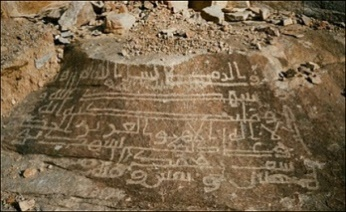
\includegraphics[width=1.57639in,height=0.96528in]{Images/image057.jpg}}{http://www.canalacademie.com/IMG/jpg/Imbert\_1\_graffiti\_SPIP.jpg}}\label{httpwww.canalacademie.comimgjpgimbert_1_graffiti_spip.jpg}}

\vide{graffiti-islamiques-du-duxe9but-de-lislam}{%
\subsubsection{{\textbf{Graffiti islamiques du début de
l'islam}
}{Graffiti islamiques du début de l'islam }}\label{graffiti-islamiques-du-duxe9but-de-lislam}}

\vide{photographie-fruxe9duxe9ric-imbert}{%
\subsubsection{{\textbf{photographie Frédéric
Imbert}}{photographie Frédéric Imbert}}\label{photographie-fruxe9duxe9ric-imbert}}

 

\paragraph{Pour aller plus loin}

Je vous propose de lire l'article de Frédéric Imbert, «~L'Islam des
pierres~: l'expression de la foi dans les graffiti arabes des premiers
siècles~», \emph{Revue des mondes musulmans et de la Méditerranée},
129~\textbar~juillet 2011. Il est consultable en ligne 

Pour vous guider dans sa lecture, une grille de questions~:

§7 et §10. Qu'est-ce que la \emph{basmala}~? Pourquoi l'auteur semble
lui accorder une certaine importance~?

§14. Pourquoi est-il intéressant de noter que la mention du Prophète est
absente~?

§19. Quelle est la thèse et l'argumentation de Y. Nevo à propos de
«~l'évidence de l'absence~»~?

De quand date la première mention du Prophète de l'islam dans un
graffito~? Quelle est sa spécificité~? \\
 

\vide{la-ux1e63aluxe2t-priuxe8re-rituelle}{%
\section{La ṣalât, prière
rituelle}\label{la-ux1e63aluxe2t-priuxe8re-rituelle}}


\vide{hommes-priant-au-caire-en-1865}{%
\mn{{ Hommes priant au Caire en
1865}}\label{hommes-priant-au-caire-en-1865}}

\vide{uxe9tymologie-1}{%
\subsection{Étymologie}\label{uxe9tymologie-1}}

La racine Ṣa.La.Wa signifie blesser au dos, arriver second à la course,
faire une action de grâce qui unit et rapproche. \textbf{Le
\emph{muṣallī}, celui qui prie, est donc toujours second, par rapport à
Celui qu'il prie.}

Si l'on réorganise la racine, on trouve Wa.Ṣa.La qui signifie atteindre,
unir, joindre~: la prière exprime ou réalise une «~jointure~» ce que le
Coran souligne dans le verset S. 33, 56~: «~Certes, Allah est Ses Anges
prient sur le Prophète ; Ô vous qui croyez priez sur lui et adressez lui
vos salutations~».

\TArabe{إِنَّ اللَّهَ وَمَلَائِكَتَهُ يُصَلُّونَ عَلَى النَّبِيِّ يَا
أَيُّهَا الَّذِينَ آَمَنُوا صَلُّوا عَلَيْهِ وَسَلِّمُوا تَسْلِيمًا}

Il existe 5 prières canoniques et selon la tradition musulmane, cette
pratique fut révélée lors de l'Ascension nocturne du Prophète, la
dixième année de sa mission.

\vide{les-cinq-priuxe8res-quotidiennes}{%
\subsection{{2.2 Les cinq prières quotidiennes
}{Les cinq prières quotidiennes }}\label{les-cinq-priuxe8res-quotidiennes}}

Pourquoi y a-t-il 5 prières en islam~? Le Coran ne dit nullement qu'il
faut prier cinq fois par jour. Il n'y est question que de deux prières.
C'est la Sunna qui va déterminer le nombre de cinq prières dans le
\emph{ḥadīṯ} du voyage nocturne du Prophète (\emph{isrāʾ}). En effet,
une nuit, le Prophète de l'islam voyagea en songe de La Mecque à
Jérusalem (voyage horizontal) auquel succéda un voyage vertical où il
monta vers les cieux, c'est l'Ascension (\emph{miʿrāǧ}) avant de
descendre aux enfers en compagnie de l'ange Gabriel sur une monture
nommée Burāq.

Selon la tradition, l'évènement s'est déroulé deux ans avant l'hégire.
La mention se trouve dans S.17, 1~: «~Gloire à celui qui a fait voyager
de nuit son serviteur de la Mosquée sacrée à la Mosquée très éloignée
dont nous avons béni l'enceinte, et ceci pour lui montrer certains de
nos Signes~». Dieu est celui qui entend et qui voit parfaitement, mais
le descriptif nous est racontée et commentée dans la Sunna. Il a donné
lieu de à de nombreuses interprétations. Nous aurons l'occasion d'y
revenir. Remarquez au passage que le Coran ne parle pas explicitement de
Muḥammad.

Voici le récit en question~concernant l'institution des 5 prières :

\begin{quote}
«~Dieu me révéla, alors ce qu'Il voulut, et prescrivit l'accomplissement
de cinquante prières par jour.

Je retournais voir Moïse (Moussa) qui me demanda : "Qu'est-ce qu'a
prescrit le Seigneur à ta Communauté?". - "Une cinquantaine de prières",
lui dis-je. - "Retourne à ton Seigneur et demande-Lui la réduction de ce
nombre, car ta Communauté ne supportera point cette prescription. Je
connais bien les israélites; je les avais mis à l'épreuve et je m'étais
employé à les ramener sur la bonne voie".

Le Prophète poursuivit : Je retournai à mon Seigneur et je Lui demandai
de réduire le nombre des prières pour la faveur de ma Communauté. Il
m'exauça en les amoindrissant de cinq prières. J'allai ensuite trouver
Moïse (Moussa) pour l'informer de la réduction à cinq prières.
Toutefois, il me répéta : "Retourne à ton Seigneur et demande-Lui la
réduction de ce nombre, car ta Communauté ne le supportera point".

Je ne cessai alors de faire la navette entre mon Seigneur (à Lui la
puissance et la gloire) et Moïse (Moussa) (que la paix soit sur lui)
pour demander plus de réduction encore jusqu'à ce que Dieu me décréta:
"Ô Muḥammad ! Je prescris irrévocablement cinq prières jour et nuit,
dont chacune équivaut à dix, cela fait alors cinquante. Quiconque a
dessein de faire une bonne action et ne la fait pas, on lui inscrira une
récompense à son actif; s'il l'exécute, une récompense équivalente à dix
bonnes actions lui sera inscrite. Tandis que quiconque a l'intention de
perpétrer une mauvaise action et qu'il ne l'accomplit pas, rien ne sera
inscrit à son passif; si au contraire il l'accomplit, on lui inscrira la
punition d'une seule mauvaise action".\\
Je redescendis et arrivai auprès de Moïse (Moussa) (que la paix soit sur
lui) pour l'informer de la situation, mais il me dit : "Retourne à ton
Seigneur et demande-Lui une nouvelle réduction".

- "Je suis déjà retourné plusieurs fois à mon Seigneur, jusqu'à ce que
j'aie trouvé inconvenant de Lui adresser encore une fois cette demande."
répondis-je à Moussa~»\sn{Ce \emph{ḥadīṯ} est rapporté par Muslim,
  \emph{Ṣaḥīḥ}, n°234.}.
\end{quote}

Les 5 prières quotidiennes sont~:

\begin{itemize}
\item
  La prière de l'aube (\emph{al-faǧr})
\item
  La prière de la mi-journée (\emph{al-ḏuhr})
\item
  La prière de l'après-midi (\emph{al-`aṣr})
\item
  La prière du coucher de soleil (\emph{al-maġrib}) {[}Vous retrouvez
  Maghreb\ldots{} et oui, c'est l'Occident, là où le soleil se couche~:
  donc ce n'est pas très positif\ldots la lumière vient de l'orient
  alors que l'occident apporte\ldots{} enfin, vous avez compris{]}.
\item
  La prière du soir (\emph{al-ʿišāʾ})
\end{itemize}

À maintes reprises, le Coran insiste sur l'importance de la prière au
cours de la journée et de la nuit et sa portée spirituelle. Nous donnons
quelques-uns de ces versets~:

S.2, 186~: «~Si Mes serviteurs t'interrogent à Mon sujet, qu'ils sachent
que Je suis tout près d'eux, toujours disposé à exaucer les vœux de
celui qui M'invoque. Qu'ils répondent donc à Mon appel et qu'ils aient
foi en Moi, afin qu'ils soient guidés vers la voie du salut.~»

S. 11, 114~: «~Accomplis la salat aux deux extrémités du jour et à
certaines heures de la nuit~».

S. 17, 78~: «~Accomplis la \emph{ṣalāt} au déclin du soleil jusqu'à
l'obscurité de la nuit et fais aussi la lecture à l'aube.~»

S. 24, 36~: «~Dans les maisons qu'Allah a permis que l'on élève (son
nom) et où son nom est invoqué. Que l'on y glorifie en elles matin et
soir.~»

S. 73, 2-7~: «~Lève-toi (pour prier) toute la nuit, excepté une partie,
sa moitié ou un peu moins ou un peu plus. Et récite le Coran lentement
et clairement\ldots La prière pendant la nuit est plus efficace et plus
propice pour la récitation. Tu as dans la journée à vaquer à des longues
occupations.~»

\vide{les-conditions-uxe0-la-priuxe8re}{%
\subsection{{Les conditions à la prière
}}\label{les-conditions-uxe0-la-priuxe8re}}

La prière doit s'effectuer dans un lieu propre. De même, le priant doit
s'assurer de la propreté de ses habits qui doivent recouvrir son corps.
Pas de tenue indécente pour prier.

Dans une mosquée, le fidèle doit tourner son visage vers la direction de
La Mecque~: c'est la \emph{qibla}. Une petite niche appelée
\emph{mihrab} la lui indique.

\vide{mihrab-dans-la-mosquuxe9e-grande-de-cordoue}{%
{{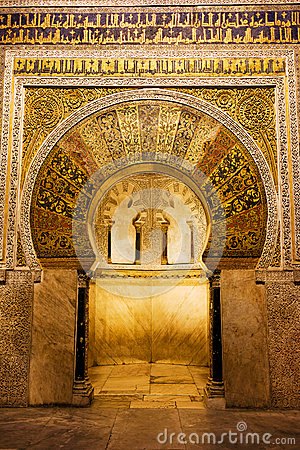
\includegraphics[width=1.40972in,height=2.11458in]{Images/image059.jpg}}{Mihrab dans la mosquée grande de Cordoue}}\label{mihrab-dans-la-mosquuxe9e-grande-de-cordoue}}

\vide{section-29}{%
\subsubsection{{ }{ }}\label{section-29}}

\vide{mihrab-de-cordoue}{%
\mn{{ Mihrab de
Cordoue}{ Mihrab de Cordoue}}\label{mihrab-de-cordoue}}

Il doit précéder sa prière en accomplissant ses ablutions. Elles ont
gagné une certaine importance dans le rite, comme en témoigne le
\emph{ḥadīṯ}~: «~l'ablution est la moitié de la foi~»\sn{~\emph{Ḥadīṯ
  ṣaḥiḥ} rapporté par Muslim ( n°223), Al-Tirmiḏī (n°3517), An-Nasa'ī (
  5/5-6), Ibn Māǧa ( 280 )\label{theol:IbnMaga1}, Ibn Hanbal dans \emph{al-Musnad}.}. Pour cela, il utilise de l'eau, ou à défaut
du sable.

Enfin, il doit formuler l'intention (\emph{niyya}) de faire la prière.
Elle témoigne de la pleine conscience de ce qu'il accomplit.

Que dit al-Ġazālī \label{theol:AlGazali11} de la pratique de la purification~?

Il distingue quatre sens dans ce rituel (Livre 3 de l'\emph{Ihyā'}) :

\begin{itemize}
\item
  la purification extérieure de toute forme de déchets ou de souillures
  diverses. Il s'agit de se purifier des déchets du corps.
\item
  la purification des péchés et des fautes accomplies par le corps
\item
  la purification du cœur de ses vices et de ses mauvais penchants
\item
  la purification du secret intime de tout ce qui n'est pas Dieu.
\end{itemize}

Al-Ġazālī \label{theol:AlGazali12} souligne l'importance de la purification du cœur, de la
purification de toute trace d'idolâtrie à l'époque du Prophète. Or, il
parle de l'obsession de la purification extérieure qui a saisi ses
contemporains et qui est paradoxalement bien loin de celle des Anciens
qui était beaucoup plus profonde. Il parle à cet égard de «~l'idiotie de
la propreté~».

La prière est difficile et la \emph{niyya} ne suffit pas toujours à
garder une concentration fermement tournée vers Dieu. Al-Ġazālī \label{theol:AlGazali13} évoque
les pensées qui sont comme des mouches. De même, la grande mystique de
l'islam Rābi`a disait~: «~Mon Dieu, quand je fais la \emph{ṣalāt},
éloigne de mon cœur toutes les suggestions sataniques (\emph{wasāwis
al-šaytān}), ou alors, par un effet de Ta bonté (\emph{mann}) et de ta
générosité (\emph{karam}), accepte mes prières même troublées par ces
suggestions~»\sn{ʿAttār, \emph{Taḏkīrat al-Awliyā}, cité par
  Badawī p. 157, dans Jean Annestay, p. 101.}.

En islam, \emph{waswas} signifie susurrer à l'oreille, suggérer. Cela
renvoie parfois à une obsession.

\vide{comment-faire-la-priuxe8re}{%
\subsection{{Comment faire la prière~?
}}\label{comment-faire-la-priuxe8re}}

Chaque prière est constitué de la répétition d'un cycle appelé
\emph{rakat}.

Si c'est la première rakat, il s'agit de prononcer la formule
\emph{Allāhu akbar} (\emph{takbīr,} c'est-à-dire c'est le fait de
prononcer cette prière), c'est-à-dire Dieu est plus grand (que tout).
Les mains sont levées au niveau des oreilles et les doigts sont joins.

\vide{httpsupload.wikimedia.orgwikipediacommons44ftakbir_of_prayer.jpg}{%
\mn[
]{\vide{\protect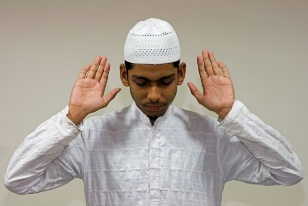
\includegraphics[width=1.38741in,height=0.92708in]{Images/image060.jpg}
}{https://upload.wikimedia.org/wikipedia/commons/4/4f/Takbir\_of\_prayer.jpg }}\label{httpsupload.wikimedia.orgwikipediacommons44ftakbir_of_prayer.jpg}}

Puis il pose la main droite sur sa main gauche au niveau du nombril et
il récite une invocation.

Il demande protection à Dieu avant de réciter la sourate
\emph{al-Fātiha}. Vous vous souvenez, c'est la première sourate du
Coran.

Ensuite, il se prosterne, et en s'abaissant il dit \emph{Allahū akbar.}
Cette position se nomme \emph{ruku}. Il invoque Dieu, puis se redresse,
lève les mains vers les oreilles, puis les rabaisse. Puis il se
prosterne. Cette position se nomme \emph{suǧud}.

\vide{sujud}{%
\mn{{\emph{sujud}}{sujud}}\label{sujud}}

Puis, il s'assoit sur ses genoux et invoque le pardon de Dieu. Il se
prosterne de nouveau et se redresse.

L'ensemble de ce rite s'appelle une \emph{raka}. Il faudra en faire une
ou deux autres.

Pour conclure la prière, le priant salut l'ange de droite et de gauche,
ces anges qui comptabilisent ces bonnes et mauvaises actions pour le
jour du jugement.

Il existe des différences selon les écoles juridiques. Par exemple, le
fait de voir les musulmans se toucher les pieds dans la mosquée est une
prescription du wahhabisme qui date du 18\textsuperscript{ème} siècle~!
Or, elle se généralise, ce qui atteste d'une wahhabisation de l'islam.

Ci-dessous une vidéo récapitulant les gestes, les positions, les paroles
prononcées.

Dans cette explication, beaucoup de choses à remarquer\ldots{} notamment
sur la diversité du rite selon les écoles juridiques (\emph{maḏhab}).

Il est question aussi à plusieurs reprises d'un ouvrage~: \emph{La
citadelle du musulman} qui est un recueil d'invocations selon les
situations de la vie.

À certains moments de la journée, il \textbf{est interdit de faire sa
prière}. Il y aurait là une pédagogie divine. En effet, al-Ġazālī \label{theol:AlGazali14} note
que ce qui est interdit est bien souvent un excitant. De même, les
gestes des différentes postures sont pédagogiques et visent à atténuer
le risque d'ennui. C'est parce que l'on accomplit la prière selon ce
rituel que se polie le cœur.

\emph{Un Récit autour de la prière}

Exemple de Hātim Asamm (le sourd), m. 237/85 \sn{~pour l'anecdote, on l'appelle ainsi,
parce qu'un jour où une vieille femme était venue le consulter, elle
laissa échapper une éructation (expulsion d'un gaz du tube digestif par
la bouche). Pour ne pas embarrasser la femme, il lui demanda de parler
plus fort car il n'entendait pas. La femme fut rassurée, mais pour ce
motif, il joua au sourd 18 années durant, jusqu'à la mort de cette
femme.
}

Donc, «~On lui demandait comment il faisait la prière. Il dit~:
«~D'abord, je purifie mon corps en le lavant avec de l'eau, en même
temps que je lave mon cœur avec la pénitence en faisant une purification
interne. Ensuite, je me rends à la mosquée. En elle je vois la Kaaba, de
même que dans la niche de prière (\emph{mihrāb}) je vois le lieu où se
tenait Abraham. Je distingue à ma droite le Paradis, à ma gauche
l'Enfer, le pont du Sirāt sous mes pieds, Azrā'īl l'ange de la mort
derrière moi. Alors je remets mon cœur à la garde de Dieu, et prononçant
la formule d'entrée en prière `Dieu est grand' (\emph{takbīr}), je joins
mes mains pour la prière, que je fais debout, dans une attitude
suppliante~; je récite le Coran avec soin, je me prosterne en toute
humilité, je reste assis avec persévérance en état d'oraison, et je
finis par l'action de grâce et la salutation~»\sn{\emph{Le
  mémorial des saints}, p. 228-233.}.

\vide{la-zakux101t-limpuxf4t-religieux-purificateur}{%
\section{La zakāt, l'impôt religieux
purificateur}\label{la-zakux101t-limpuxf4t-religieux-purificateur}}



\vide{uxe9tymologie-2}{%
\subsection{Étymologie}\label{uxe9tymologie-2}}

C'est un impôt légal, obligatoire à distinguer de l'aumône libre
\emph{ṣadaqa}.

Étymologiquement, il signifie purifier, croître, prélever.

Cet impôt est lié à la prière~: 
\begin{quote}
    
«~Acquittez-vous de la prière, faites
l'aumône~» (S. 2, 43).
\end{quote}
\vide{bienfaits-de-la-zakux101t}{%
\subsection{{ Bienfaits de la
\emph{zakāt}}}\label{bienfaits-de-la-zakux101t}}

Son but est la circulation des biens et sa répartition équitable. Il
s'agit de faire circuler ce qui est excédent ou superflu~:

\begin{quote}
«~Ils t'interrogent au sujet de ce qu'ils doivent distribuer~? Réponds~:
le superflu~» (S. 2, 219).
\end{quote}

La \emph{zakāt} répond à la nécessité d'enlever l'excédent improductif.
C'est une sorte d'impôt sur la fortune. La \emph{zakāt} doit purifier le
croyant lui-même~: tout est à Dieu. Il doit être responsable devant la
communauté de ce qu'il détient. Ses modalités sont assez complexes et
varient selon les jurisprudences. Initialement, elle ne portait que sur
l'or et l'argent, le bétail, les céréales. Il faut signaler que l'islam
interdit que la monnaie engendre la monnaie et condamne le taux à
intérêt.

Spirituellement, la \emph{zakāt} vise à éprouver le croyant qui prétend
aimer Dieu. Si tu aimes Dieu, alors donne ton superflu. Elle prévient
aussi du danger de prendre l'argent pour Dieu~: elle permet de purifier
le \emph{tawhīd}. C'est-à-dire l'Unicité. Cependant, la \emph{zakāt} ne
doit pas être l'occasion de s'enorgueillir. Il ne faut pas s'en
acquitter publiquement, ce qui constitue aussi une humiliation pour le
pauvre. Le véritable bienfaiteur, ce n'est pas celui qui donne, mais
celui qui reçoit, car il permet à celui qui donne de s'acquitter de ce
qu'il doit donner pour purifier son cœur.

Il s'agit de donner ce qui est licite et ce qui est le plus cher à ses
yeux~: «~Ne choisissez pas ce qui est vil pour donner en \emph{zakāt} »
(S. 2, 267).

\vide{uxe0-qui-donner-la-zakux101t}{%
\subsection{{À qui donner la \emph{zakāt} ?
}}\label{uxe0-qui-donner-la-zakux101t}}

Pour al-Ġazālī \label{theol:AlGazali15}, il faut s'assurer que la personne appartienne à l'une de
ces catégories~:

\begin{itemize}
\item
  elle a la crainte révérencielle~: donc aux pieux, afin de les aider
  dans leur vie spirituelle.
\item
  elle a la science~: donner aux savants, cela contribue à la
  propagation de la foi et de la Loi.
\item
  elle a le sens de la cause première~: autrement dit, elle voit dans le
  don, la manifestation de Dieu. Elle ne s'arrête pas aux moyens, aux
  causes secondes, à la main humaine qui a donné. Cela ne veut pas dire
  qu'elle ne remercie pas le donateur. C'est même une obligation~: celui
  qui n'a pas remercié le donateur n'a pas remercié Dieu.
\item
  elle doit cacher sa pauvreté, ne pas se plaindre.
\item
  elle doit avoir une famille, ou être atteint d'une maladie, croupir
  sous les dettes. La \emph{zakāt} doit lui permettre de sortir de la
  gêne.
\item
  elle doit faire partie des proches et de ceux qui sont liés par le
  sang.
\end{itemize}

\vide{ux1e63iyux101m-et-ux1e63awm-le-jeuxfbne}{%
\section{ṣiyām et ṣawm~: le
jeûne}\label{ux1e63iyux101m-et-ux1e63awm-le-jeuxfbne}}


\vide{ramaux1e0dux101n-mubux101rak}{%
\subsubsection{{\emph{Ramaḍān
mubārak}}{Ramaḍān mubārak}}\label{ramaux1e0dux101n-mubux101rak}}

\vide{duxe9finitions-et-uxe9tymologie}{%
\subsection{Définitions et
étymologie}\label{duxe9finitions-et-uxe9tymologie}}

L'étymologie est intéressante. ṢaWaMa signifie s'abstenir, renoncer à,
s'interdire, se taire, se radoucir en parlant du vent, atteindre le
zénith. Le jeûne a été prescrit au mois de Ramaḍan. Or, RaMaDa renvoie à
l'idée de rôtir, de brûler, d'embraser, d'être brûlant.

\begin{Def}[jeûne]
Le jeûne est donc l'abstention, le silence, l'adoucissement pour
tempérer et neutraliser le feu du mois de Ramadan.
\end{Def}

\mn{Le grand moment liturgique~: c'est le ramadan. On relit le Coran.}
Mais le mois de Ramadan n'est pas qu'affaire de jeûne. Au cours de ce
mois, le musulman est invité à suivre des retraites spirituelles,
notamment les dix derniers jours. Une tradition rapporte~:
\begin{quote}
    «~Dès que
commencent les dix dernières nuits de Ramadan, l'Envoyé de Dieu se
serrait la ceinture, veillait la nuit en dévotion et réveillait les gens
de sa maison~»
\end{quote}. Selon les savants, l'expression «~se serrer la
ceinture~» signifie se détourner des femmes pour montrer tout le sérieux
dans son action spirituelle.

Le but du jeûne est donc spirituel~: parce que l'homme est une créature
entre l'animal et l'ange, s'il se soumet à ses passions, il et ramené à
l'état bestial, mais s'il les combat, il s'élève à celui des anges car
supporter la faim et la soif est un attribut de Dieu et des anges.

\vide{diffuxe9rents-types-de-jeuxfbne}{%
\subsection{4.2 Différents types de
jeûne}\label{diffuxe9rents-types-de-jeuxfbne}}

\emph{Ṣiyām} qualifie le jeûne obligatoire~; c'est le jeûne légal de
prescription divine. Il est un exercice de soumission volontaire, le
bouclier de la chasteté quand on ne peut pas se marier~; le jeûne
consiste aussi en l'abstention de tout mal, en paroles et en actes.

Al-Ġazālī \label{theol:AlGazali16} distingue trois sortes de jeûnes~:

\begin{itemize}
\item
  Le jeûne des gens du commun~: on s'abstient de manger ou de boire,
  d'avoir des rapports sexuels.
\item
  le jeûne des gens de l'élite~: empêcher le regard, la langue, la main,
  le pied, l'ouïe, la vue et l'ensemble des membres de commettre des
  péchés.
\item
  le jeûne de l'élite de l'élite~: c'est le jeûne du cœur devant les
  basses ambitions et les idées qui éloignent de Dieu.
\end{itemize}

Le jeûne n'est pas purement abstinence~: il est associé à la nécessité
de la réconciliation, de la générosité, de l'hospitalité. On peut citer
à cet égard le \emph{ḥadīṯ}~suivant : \emph{«~Pour celui qui ne renonce
pas au mensonge dans les actes et les paroles, Dieu n'a nul besoin qu'il
renonce à sa nourriture et à sa boisson}~».

\emph{ṣawm} qualifie le jeûne libre. Le jeûne n'est pas spécifique au
mois du Ramadan. Les musulmans sont invités à jeûner au début et à la
fin de chaque mois, ou trois jours au milieu. On doit aussi jeûner le
jour de \emph{ʿarafāt} ou de \emph{ʿāšūrāʾ}. Vous ne connaissez pas ces
deux mots. Pas de panique. Cela viendra et je vous enverrai un petit
pensum\ldots{}

Le jeûne a une dimension spirituelle. Il est abstention et attitude
intérieure. Il va faire ressortir dans l'être un certain nombre
d'appétits, de dispositions, de traits de caractère qui ne sont pas
conformes à une orientation tournée vers Dieu seul. Il va révéler les
tendances troubles qui sont en nous, les tendances troubles de l'âme qui
sommeillent et nous trompent. Le jeûne va donc purifier l'être, le
rendre transparent comme un diamant afin de rendre présent Dieu seul.

Si vous lisez le livre qu'al-Ġazālī \label{theol:AlGazali16} consacre au jeûne, vous verrez qu'il
critique la tendance de certains de sa communauté à s'abstenir
d'aliments et de boissons dans la journée mais à s'empiffrer dès que le
soleil est tombé. Il y a pour le savant une profonde méprise et
perversion du rite.

\vide{le-puxe8lerinage-le-ux1e25aux11fux11f}{%
\section{{Le pèlerinage~: le \emph{ḥağğ}
}}\label{le-puxe8lerinage-le-ux1e25aux11fux11f}}


\vide{uxe9tymologie-3}{%
\subsection{{ Étymologie
}}\label{uxe9tymologie-3}}

La racine Ḥa Ğa Ğa signifie se diriger vers, se proposer, l'emporter
dans l'argumentation sur quelqu'un.

Le \emph{ḥağğ} est donc une quête. Il regroupe l'ensemble des actes
accomplis au cours du Pèlerinage. Il correspond au Pèlerinage que
Muḥammad a accompli en l'an dix de l'Hégire, quelques mois avant sa
mort, avec 140~000 musulmans. C'est le Pèlerinage de l'Adieu,
\emph{ḥiğğat al-Wadā`.} Le neuvième jour du douzième mois, fut révélé à
Muḥammad le verset suivant~: «~Ce jour, j'ai parachevé pour vous votre
religion. J'ai parachevé mon Bienfait à votre égard et j'agrée pour vous
l'islam comme religion~» (S. 5, 3).

La révélation a lieu à Arafat, situé en dehors du territoire sacré.

Le \emph{ḥaǧǧ} est une obligation pour tout musulman qui en a les
moyens.

On distingue le petit \emph{ḥağğ} du grand \emph{ḥağğ}~: le premier est
fait n'importe quand dans l'année tandis que le second est effectué
seulement pendant le mois du Ramaḍān.

\vide{conditions-requises-uxe0-laccomplissement-du-ux1e25aux11fux11f}{%
\subsection{{Conditions requises à l'accomplissement
du \emph{ḥağğ}
}}\label{conditions-requises-uxe0-laccomplissement-du-ux1e25aux11fux11f}}

\begin{itemize}
\item
  Des dépenses d'origine licite
\item
  Ne pas aider les ennemis de Dieu en leur versant des droits d'entrée
\item
  Des dépenses faites avec parcimonie
\item
  La chasteté est de rigueur dans les propos~: on doit s'encourager, se
  stimuler spirituellement.
\item
  Se préparer au grand voyage, comme si on n'allait pas revenir.
\end{itemize}

\vide{le-rituel}{%
\subsection{Le rituel}\label{le-rituel}}

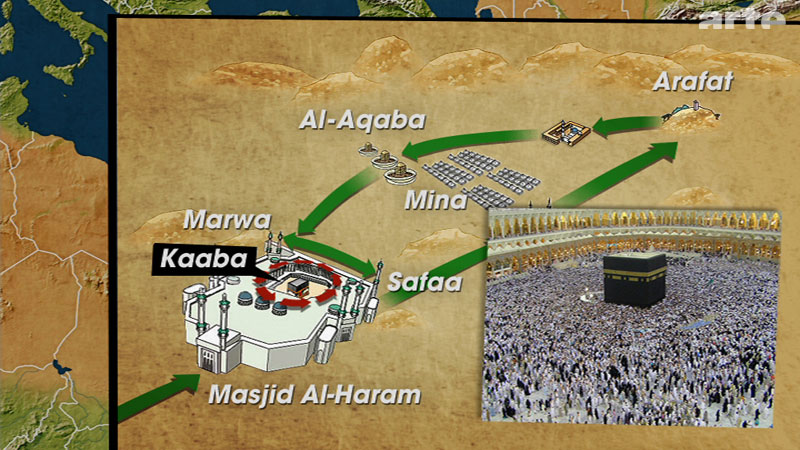
\includegraphics[width=5.51181in,height=3.09931in]{Images/image066.jpg}

Tout commence à la limite du territoire sacré. On exprime la
\emph{niyya}. Le mot a été rencontré à propos de la prière. Quand on
commence à faire la prière, il faut formuler la \emph{niyya}
c'est-à-dire\ldots~? Allez, un petit effort, je suis sûr que vous le
savez.

Puis, il s'ensuit un rituel vestimentaire et corporel qui donne le
statut d'\emph{iḥrām}, c'est-à-dire de consécration. On procède à la
grande ablution. Puis on revêt un vêtement composé de deux pièces
d'étoffes blanches non cousues.

On ne doit pas se couper les cheveux, s'épiler, se couper les ongles, se
couvrir la tête pour l'homme, chasser ou avoir des relations sexuelles.

Le pèlerin va vers la Kaaba, temple selon la tradition musulmane
construit par Adam, reconstruit par Abraham. On y trouve la pierre noire
(blanche à l'origine, mais devenue noire à cause des péchés des hommes.
Sur cette pierre, il existe plusieurs légendes).

Le pèlerin marche autour du Temple. Sa déambulation se dénomme
\emph{tawaf}. À l'approche de la Mosquée, il lève les deux bras vers le
Ciel et répète~: \emph{Labbayka Allahouma Labbayka} (Me voici, ô mon
Dieu, me voici).

Dans la mosquée, il doit toucher la pierre noire, ou faire un geste en
sa direction.

Le fidèle fait 7 fois le tour de la Kaaba, trois rapides et 4 lents dans
le sens inverse des aiguilles d'une montre. C'est la giration autour du
centre de l'univers.

Puis vient le \emph{say}, ou course angoissée d'Agar. Agar est cette
femme, servante de Sarah, qui fut chassée par sa maîtresse. Elle dut
fuir dans le désert, avec dans ses bras son enfant, Ismaël. Elle cherche
de l'eau, puis surgit la source de Zemzem. Le pèlerin accomplit cette
marche entre deux rochers distants de 400m, Safa et Marwa. Il doit faire
la course 7 fois. À la fin, il boit de l'eau de Zemzem.

Ces rites accomplis, on entre dans le cœur du pèlerinage. C'est le 8 de
\emph{Dhou al-hijja}, le dernier mois de l'année lunaire. Le pèlerin se
rend à pied à Mina, à 7 km de La Mecque et il y campe. Il reçoit le
pardon de Dieu (\emph{woukouf}). Il marche vers la plaine d'Arafat à 12
km. À midi, station debout prolongée où le pèlerin reçoit le pardon de
Dieu au pied du mont de la Miséricorde (\emph{Ğabal al-Raḥma})~: c'est
de là que Muḥammad s'adressa aux fidèles lors de son pèlerinage d'Adieu.
C'est le point culminant du pèlerinage. Puis on revient sur ses pas, le
soir, on s'arrête à Mouzdalifa pour y passer la nuit. Là, on ramasse les
49 petits cailloux pour les lapidations rituelles des stèles
représentant le démon.

C'est l'\emph{Aïd al-Ada} ou la fête du sacrifice d'Abraham.

Le 10 du mois, avant l'Aube, on se rend à Mina pour une lapidation
symbolique et pour y sacrifier un animal. C'est l'\emph{Aïd al-Kebir}.
Après le sacrifice, le pèlerin se coupe les cheveux ou se les rase.

Le \emph{Tawaf} est la marche d'Adieu autour du Temple. Le 11 et le 12
ont lieu d'autres lapidations symboliques. Les fidèles reviennent à La
Mecque pour la circumambulation de l'Adieu autour de la Kaaba. Le
pèlerinage est fini. Certains le complètent par un voyage à Médine.

\vide{conclusion-1}{%
\section{Conclusion~}\label{conclusion-1}}

Pour conclure, une histoire, celle d'un dialogue entre Moïse et Dieu et
qui tend à minimiser l'importance de ces 5 piliers pour privilégier la
voie de l'amour mais aussi celle de l'aversion.

\begin{quote}
«~On rapporte que Dieu a révélé à Moïse~: «~As-tu jamais accompli une
œuvre pour Moi~? Moïse répondit~: Mon Dieu~! J'ai prié devant Toi~; j'ai
jeûné, j'ai fait l'aumône légale~! Dieu lui dit~: la prière est pour toi
une preuve (burhān), le jeûne une armure (ğunna), l'aumône est un abri
(ẓill), l'impôt légal une lumière (nūr). Mais quelle œuvre as-tu fait
pour Moi~? Moïse dit~: Mon Dieu~! Indique-moi quelle est l'œuvre qui
soit à Toi~? Dieu lui dit~: Ô Moïse, as-tu jamais pris un ami pour moi~
et en animosité un ennemi pour Moi~? Moïse sut alors que la meilleure
œuvre c'est l'amour en Dieu et l'aversion en Dieu~»\sn{Al-Ġazālī \label{theol:AlGazali9}\emph{,
  Les règles de l'amitié et de la fraternité en Islam}, (K. 15, ar. p.
  593~; fr. p. 19) {[}notre traduction{]}.}.
\end{quote}

\textbf{Pour aller plus loin~:}

On pourra lire le récit passionnant d'Abdallah Hammoudi, anthropologue
et enseignant à Princeton~: \emph{Une saison à La Mecque}, Paris, Seuil,
2005. Il s'agit à la fois d'une démarche de croyant et d'anthropologue.
Mais les deux sont-ils compatibles~? À son retour au Maroc, Hammoudi
refusera le titre de \emph{hāǧ} que l'on attribue à celui qui revient de
pèlerinage. Un signe manifeste de la difficulté qu'il a rencontrée à
concilier la démarche scientifique, objective, observatrice, et sa
participation comme musulman.

\vide{httpwww.seuil.comimagescouvm9782020669801.jpg}{%
{{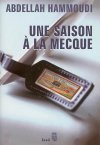
\includegraphics[width=1.04167in,height=1.51389in]{Images/image067.jpg}}{http://www.seuil.com/images/couv/m/9782020669801.jpg}}\label{httpwww.seuil.comimagescouvm9782020669801.jpg}}



\chapter{Les croyances musulmanes}

\vide{introduction-2}{%
\section{{Introduction}}\label{introduction-2}}

S'il n'existe pas en islam de magistère, il existe un genre littéraire
appelé \emph{ʿaqīda}, \textbf{\TArabe{عقيدة}} (pluriel~: ʿ\emph{aqāʾid}),
c'est-à-dire \textbf{profession de foi}. Contrairement au christianisme
où le credo est élaboré dans le cadre d'un synode, en islam, ce sont les
savants qui rédigent au cours de leur vie, parfois sur leur lit de mort,
ce en quoi ou à quoi ils croient. C'est le résumé de leur foi.

Ces professions de foi qui reposent sur le Coran et la Sunna sont
d'abord sommaires, mais elles connaissent dans le temps un développement
qui témoigne de l'élaboration progressive d'un \emph{credo} commun et de
la définition d'une «~orthodoxie~». Si la \emph{šahāda} définit
l'attestation d'adhésion à l'islam, la profession de foi précise la
nature des croyances afférentes. Ces professions permettent de délimiter
un cadre de croyances et de lutter contre des idées considérées comme
\textbf{innovation} (\emph{bidʿa}, \TArabe{بدعة}). Elles délimitent ainsi
les frontières de «~l'orthodoxie~». En fonction des questions
théologiques qui sont posées, des contextes particuliers, des outils
philosophiques utilisés, les réponses diffèrent d'une profession de foi
à l'autre mettant en lumière à la fois un islam pluriel mais aussi la
propension à revendiquer le monopole de l'orthodoxie en excluant celui
qui ne partage pas le Credo défini (C'est la pratique du \emph{takfīr}
que nous avons déjà rencontrée et qui consiste à anathémiser l'autre).
L'influence des débats avec les juifs et les chrétiens ou celle de juifs
et de chrétiens convertis a contribué au développement de ces
professions de foi en apportant avec eux à la fois des questions
théologiques mais aussi une argumentation pour appréhender les réponses.

Dans cette leçon, nous présenterons dans un premier temps les grandes
croyances musulmanes, puis nous exposerons quelques-unes de ces
professions de foi afin de mettre en exergue leur développement.

\vide{i--les-principales-croyances-musulmanes}{%
\section{Les principales croyances
musulmanes}\label{i--les-principales-croyances-musulmanes}}

Le verset S. 2, 177 est traditionnellement considéré comme répertoriant
les cinq grandes vérités du \emph{credo} musulman (\emph{al-ʿaqīda})~:
Dieu, les anges, les prophètes, les Écritures et l'eschatologie. On
parle à cet égard des cinq piliers de la foi.

À distinguer bien sûr des cinq piliers de l'islam qui renvoient à une
pratique. Il s'agit des cinq principaux thèmes retenus par les manuels
de \emph{kalām} (la théologie défensive) auxquels certains ajoutent la
prédestination (\emph{qadar}) en suivant le deuxième \emph{hadīṯ qudsī}
de Nawāwī et d'autres la direction de la communauté (\emph{imāma}). Donc
les 5 peuvent être 6\ldots{}

Avant d'aller plus loin et d'exposer le verset coranique et le
\emph{ḥadīṯ qudsī}, une petite explication s'impose~: qu'est-ce donc
qu'un \emph{ḥadīṯ qudṣī}~? Vous savez ce qu'est un \emph{ḥadīṯ}~: une
parole ou un geste prophétique. Vous savez aussi que l'on a qualifié les
\emph{ḥadīṯ} selon la chaîne de transmetteurs (\emph{isnād})~: certains
sont dits faibles, d'autres bons, d'autres encore authentiques\ldots{}
mais il y a aussi un type de \emph{ḥadīṯ} appelé \emph{qudsī},
c'est-à-dire «~sacré~». On retrouve la racine QaDaSa (\emph{kadosh} en
hébreu). Ces \emph{ḥadīṯs} sont des paroles du Prophète Muḥammad mais
attribuées à Dieu, c'est-à-dire que Muḥammad y rapporte une parole de
Dieu. Pour autant, cette parole n'est pas issue du Coran.

\begin{itemize}
\item
  Le texte de S.2, 177~:
\end{itemize}

\begin{quote}
«~La bonté pieuse ne consiste pas à tourner vos visages vers le Levant
ou le Couchant. Mais la bonté pieuse est de \textbf{croire en Allah, au
Jour dernier, aux Anges, au Livre et aux prophètes,} de donner de son
bien, quelque amour qu'on en ait, aux proches, aux orphelins, aux
nécessiteux, aux voyageurs indigents et à ceux qui demandent l'aide et
pour délier les jougs, d'accomplir la Salat et d'acquitter la Zakat. Et
ceux qui remplissent leurs engagements lorsqu'ils se sont engagés, ceux
qui sont endurants dans la misère, la maladie et quand les combats font
rage, les voilà les véridiques et les voilà les vrais pieux~!~»
\end{quote}

\TArabe{لَيْسَ الْبِرَّ أَنْ تُوَلُّوا وُجُوهَكُمْ قِبَلَ الْمَشْرِقِ
وَالْمَغْرِبِ وَلَكِنَّ الْبِرَّ مَنْ آَمَنَ بِاللَّهِ وَالْيَوْمِ
الْآَخِرِ وَالْمَلَائِكَةِ وَالْكِتَابِ وَالنَّبِيِّينَ وَآَتَى الْمَالَ
عَلَى حُبِّهِ ذَوِي الْقُرْبَى وَالْيَتَامَى وَالْمَسَاكِينَ وَابْنَ
السَّبِيلِ وَالسَّائِلِينَ وَفِي الرِّقَابِ وَأَقَامَ الصَّلَاةَ وَآَتَى
الزَّكَاةَ وَالْمُوفُونَ بِعَهْدِهِمْ إِذَا عَاهَدُوا وَالصَّابِرِينَ
فِي الْبَأْسَاءِ وَالضَّرَّاءِ وَحِينَ الْبَأْسِ أُولَئِكَ الَّذِينَ
صَدَقُوا وَأُولَئِكَ هُمُ الْمُتَّقُونَ}

\begin{itemize}
\item
  Le \emph{ḥadīṯ qudsī}
\end{itemize}

«~L'islam consiste à témoigner qu'Allāh est le Dieu unique et Muḥammad
son Envoyé, à s'acquitter de la prière et de l'aumône rituelles, du
jeûne de Ramadān et du pèlerinage à la Maison de Dieu, si l'on en a les
moyens~(\ldots) La foi (\emph{īmān}) consiste à croire à Dieu, ses
anges, ses écritures, ses prophètes, et au dernier Jour ainsi qu'à
croire à la prédestination au bien et au mal~»\sn{~\textsc{al-Nawawî},
  \emph{Une herméneutique de la tradition islamique : le commentaire des
  Arba‛ûn al-nawawîya de Muḥyî al-Dîn Yaḥyâ al-Nawawî (m. 676/1277)},
  Introduction, texte arabe, traduction, notes et index du vocabulaire
  par Louis Pouzet\emph{,} Beyrouth, Dar el-Machreq, 1982, p. 90,
  (traduction légèrement modifiée).}.

On trouve aussi dans le \emph{ḥadīṯ qudsī} n°4~de la même collection :

« La foi consiste en ce que tu dois croire à Allah, à Ses Anges, à Ses
Livres, à Ses Prophètes, au Jugement Dernier. Tu dois croire encore à la
prédestination touchant le bien et le mal »\sn{\textsc{al-Nawawî,}
  \emph{ḥadīṯ} n°4.}.

\vide{bibliographie-pour-une-suxe9lection-des-professions-de-foi-islamique-je-vous-conseille-deux-ouvrages}{%
\subsubsection{{\textbf{Bibliographie}~: Pour une
sélection des professions de foi islamique, je vous conseille deux
ouvrages:
}{Bibliographie~: Pour une sélection des professions de foi islamique, je vous conseille deux ouvrages: }}\label{bibliographie-pour-une-suxe9lection-des-professions-de-foi-islamique-je-vous-conseille-deux-ouvrages}}

\vide{section-33}{%
\subsubsection{}\label{section-33}}


\mn{{William Montgomery \textsc{Watt},
\emph{Islamic Creeds}, A selection, Edinburgh University Press, 2001
(1994) L'avantage de celui-ci est qu'il est en poche. Mais c'est en
anglais.}}




\mn{{Arent Jan W\textsc{ensinck}, \emph{The
Muslim Creed}, Its Genesis and Historical Development, Cambridge, 1932.
Un grand classique de l'islamologie. Vous pouvez le consulter et le lire
en ligne via
\url{https://archive.org/details/630\_The.Muslim.Creed}}}

Ce \emph{ḥadīṯ} est repris en introduction de la plupart des
ʿ\emph{aqā'id}. C'est le pluriel de \emph{ʿaqīda}, profession de foi. Je
vous l'ai signalé dans l'introduction..\emph{.} Les professions de foi
vont commenter ces articles sur la base du Coran et de la Sunna. Il
s'agit de répondre aux questions du type~:

\textbf{Qui est Dieu~? Que sait-on de lui~?}

\begin{quote}
Qu'en est-il des anges~? Quelle est la nature de ces êtres spirituels~?
Sont-ils bons~? Peuvent-ils faire le mal~?
\end{quote}

Qu'en est-il des livres~? De quels livres s'agit-il~? Sont-ils tous
égaux~?

Qui sont les Envoyés de Dieu~? Quel est leur nom~? Quelle est leur
histoire~?

\begin{quote}
Comment se déroulera le jugement de Dieu~? Est-ce que les musulmans
peuvent aller en enfer~? Et les non-musulmans~? Et l'hypocrite~? Et le
voyou~? Et le fornicateur~?
\end{quote}

Ma liberté est-elle engagée ou tout est-il déjà écrit d'avance
(\emph{maktub})~?

La \emph{ʿaqīda} répond à toutes ces questions. Mais, par là-même, elle
prend position dans le commentaire des versets mobilisés. Je ne rentre
pas dans cette leçon sur les débats théologiques. Vous avez la
possibilité au second semestre de suivre le cours d'Adrien Candiard sur
la théologie musulmane. Pour l'instant il s'agit surtout d'exposer ces
croyances. Je vais donc reprendre les 5-6 articles de foi.


\subsection{{Le \emph{tawḥīd} contre le \emph{širk}
ou la réforme perpétuelle de l'islam
}\label{le-tawux1e25ux12bd-contre-le-ux161irk-ou-la-ruxe9forme-perpuxe9tuelle-de-lislam}}

Croire en Dieu c'est comme l'atteste la \emph{šahāda} (vous savez le
premier pilier\ldots~; au fait, la lettre \emph{š} se prononce sh, vous
n'aviez pas oublié~?), croire qu'il n'y a pas d'autres dieux que Dieu.
Le seul Dieu c'est Dieu. Dieu est unique.

\begin{Def}[tawḥīd]
Cette affirmation de l'unicité
divine se nomme \emph{tawḥīd}. Elle est au cœur de la prédication
musulmane.
\end{Def}


\subsection{Calligraphie de Tawhid}


\includegraphics[width=\textwidth]{Images/image015.jpg}
« Le tawhid renvoie dans l'islam au dieu « un ». Mais la notion est
évolutive. Dans le Coran, le dieu local,~\emph{« protecteur du point
d'eau de La Mekke »}, se mue rapidement en dieu créateur, qui se suffit
à lui-même et n'a pas d'associé. C'est une manière de déligitimer les
trois déesses locales qui étaient supposées protéger les déplacements.
Plus tard, sur la coupole du Rocher à Jérusalem, construite en 692, est
inscrit un verset coranique (Sourate 4, Verset 171) qui récuse la
Trinité, faisant simplement de Jésus, « Fils de Marie », le « messager »
qui précède Mohammed. On semble être dans un défi à l'empire byzantin.
Enfin, beaucoup plus tard, au milieu du XVIII\textsuperscript{e}~siècle,
le tawhid devient un enjeu interne à l'islam avec le mouvement sectaire
du wahhabisme qui combat avec virulence les courants mystiques de
l'islam qui sont accusés « d'associer » d'autres divinités à Dieu. » \sn{Jacqueline Chabbi}



« Pour dessiner l'unité, j'ai utilisé dans cette calligraphie la forme
du carré. Lors de mes premiers essais, je faisais plutôt des cercles.
Là, j'ai déformé une des lettres (le h) pour la relier avec les autres
et les faire entrer toutes dans un carré. J'ai agrandi cette lettre
jusqu'à ce qu'elle enlace les autres lettres, comme dans un souffle. En
calligraphie, le souffle est important. Tous les calligraphes
travaillent sur le souffle. Quand on fait le geste, on coupe son
souffle. Quand on va à l'encrier, on reprend souffle. » \sn{Hassan Massoudy}



Le musulman, quand il récite la \emph{šahāda} ou quand il prêche, lève
l'index signifiant sa foi en Dieu un. À sa mort il est mis dans un
linceul, les mains jointes, et parfois, l'index droit désuni des autres
doigts de la main (parfois il est tourné vers le ciel).



\vide{adorer-dieu}{%
\subsubsection{{Adorer Dieu
}}\label{adorer-dieu}}

Affirmant que Dieu est unique, le musulman récite quotidiennement la
sourate 112 intitulée, \emph{al-iḫlaṣ} que l'on traduit souvent par «~le
culte pur~».


\begin{table}[h!]
\resizebox{\textwidth}{!}{%
\small
\begin{tabular}{p{7cm}p{7cm}}
1. Dis: «Il est Allah, Unique.
&

\TArabe{بِسْمِ اللَّهِ الرَّحْمَنِ الرَّحِيمِ}

\TArabe{قُلْ هُوَ اللَّهُ أَحَدٌ}
\\
2. Allah, Le Seul à être imploré pour ce que nous désirons.
&
\TArabe{اللَّهُ الصَّمَدُ}
\\

3. Il n'a jamais engendré, n'a pas été engendré non plus.
& 
\TArabe{لَمْ يَلِدْ وَلَمْ يُولَدْ}
\\
4. Et nul n'est égal à Lui».
&
\TArabe{وَلَمْ يَكُنْ لَهُ كُفُوًا أَحَدٌ} \\

\end{tabular}%
}
\caption{sourate 112 , \emph{al-iḫlaṣ}, «~le
culte pur~»}
\end{table}



Au cours de l'histoire, cette sourate 112 a été invoquée par des
penseurs musulmans dans le cadre de \textbf{polémiques contre les
chrétiens}. Mais il faut noter qu'elle n'était pas, à son origine,
destinée à réfuter la croyance chrétienne. Elle est un \emph{credo}
contre le polythéisme.

L'affirmation d'un Dieu unique implique pour les musulmans que Dieu
existe. Il manifeste son existence dans des signes (\emph{āyāt}, آيات),
ceux de la création, ceux du Livre qu'il a révélé.

Dire que Dieu est `un' implique que l'adoration revient à Lui seul. Seul
devant Lui le croyant se prosterne. La\emph{ʿibāda}, l'adoration, la
soumission totale, lui revient.

Si l'on refait un peu d'arabe vous voyez que la racine de \emph{ʿibāda}
est ʿa.Ba.Da. Vous la retrouvez dans le mot ʿAbd-Allāh\ldots{} qui
signifie serviteur, soumis, adorateur de Dieu.


\begin{Def}[Taghut]
{Taghut~(ar. \TArabe{طاغوت} ), ṭāġūt. Plusieurs~: Ṭawāġīt. Au sens large~: "aller au-delà de la mesure" ou désignant une "hauteur" ou un "sommet" de ṭāġiyah \TArabe{ طاغية} lit. tyran) est~une terminologie islamique~désignant un centre de culte autre que~Dieu.}
\end{Def}

La pensée musulmane est fondamentalement une pensée du Dieu unique~; la
prédication ne cessera d'attirer l'attention sur les idoles qui
s'immiscent dans l'islam au cours de l'histoire. Les grands réformateurs
de l'islam partent toujours de l'unicité divine. Ainsi, par exemple, au
XII\textsuperscript{e} siècle, la dynastie des Almohades instaurée au
Maroc s'appuie sur la doctrine d'Ibn Tumart (m.~1128). Ils se font
appeler les \emph{muwahhidūn}, c'est-à-dire les partisans de l'unicité,
les monothéistes, les unitariens.

\vide{notice-biographique-ibn-tumart-1080-1130}{%
\subsubsection{Notice biographique -- Ibn Tumart
(1080-1130)}\label{notice-biographique-ibn-tumart-1080-1130}}




C'est un personnage curieux qui après
avoir étudié en Andalousie et à Bagdad la doctrine d'al-Ašʿarī
(al-Ġazālī est aussi disciple d'al-Ašʿarī), revient dans son pays natal,
le haut Atlas et prêche un monothéisme rigoureux et réformateur. Dans
les montagnes, il va constituer un État disposant d'une armée, unie par
une doctrine religieuse rigoriste. Pour lui, toute forme de
divertissement est idolâtrie et contrevient à l'islam pur. Le \emph{dār
al-islām} (terre d'islam) ne saurait en ces conditions accueillir sur
son territoire des communautés religieuses non musulmanes. C'est de son
époque que l'on date la fin des communautés chrétiennes au Maghreb.
Ainsi, il condamne l'écoute de la musique qui éloigne de l'adoration qui
est due à Dieu. Son rigorisme moral lui attira bien des ennemis. À la
fin de sa vie, il se proclame Imam, Mahdi. Comme nous le verrons dans la
prochaine leçon, c'est une doctrine essentiellement šīʿite.


\vide{pour-plus-de-duxe9tails-vous-pouvez-lire-sa-biographie-issue-de-lencyclopuxe9die-berbuxe8re-p.3604-3606.}{%
\subsubsection{{Pour plus de détails, vous pouvez lire sa
biographie issue de \emph{l'Encyclopédie berbère}, p.3604-3606.
}{Pour plus de détails, vous pouvez lire sa biographie issue de l'Encyclopédie berbère, p.3604-3606. }}\label{pour-plus-de-duxe9tails-vous-pouvez-lire-sa-biographie-issue-de-lencyclopuxe9die-berbuxe8re-p.3604-3606.}}
 

De même, au 18\textsuperscript{ème} siècle, dans la péninsule arabique,
ʿAbd al-Wahhab entreprend une réforme de l'islam. Il s'agit avant tout
de s'attaquer à la prolifération de la superstition et de
l'associationnisme (\emph{širk}) dans la péninsule. Dans son Livre
\emph{Kitāb al-tawḥīd}, il invoque la nécessité d'adorer Dieu seul et de
rejeter le \emph{ṭāġūt} (\textbf{\TArabe{طاغوت}})\textbf{,} c'est-à-dire
tout ce qui est adoré en dehors de Dieu et qui contredit la Loi
islamique. Il y mentionne par exemple le port d'un bracelet pour
conjurer le mal, le port de talisman, etc.

Aujourd'hui, la propagande de Daesh a témoigné qu'il s'agit aussi d'un
mouvement unitarien rigoriste. L'État islamique est dans la même ligne
que celle d'un Ibn Tumart. La destruction des mausolées, des statues
antiques, des mosquées abritant le tombeau de saints sont les
conséquences de l'affirmation du \emph{tawḥīd} tel que défini par ʿAbd
al-Wahhab dans son \emph{Livre de l'unicité divine}~: pour lui, il ne
suffit pas d'affirmer que Dieu est unique (\emph{tawḥīd al-rubūbiyya})~;
cette affirmation doit aussi se mettre en œuvre dans la pratique en
n'adorant que Dieu seul (\emph{tawḥīd al-ulūhiyya}) et en combattant
toute forme d'idolâtrie. La croyance en l'intercession des prophètes ou
des saints sont vues comme autant de formes d'associationnisme à
combattre. D'où la destruction des mausolées.

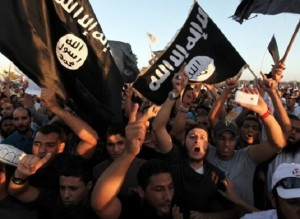
\includegraphics[width=3.11458in,height=2.28125in]{Images/image072.jpg}

\begin{quote}
\emph{Partisans de l'État islamique, l'index levé}

\emph{Les drapeaux mentionnent la šahāda}
\end{quote}

\vide{ux2bfabd-al-wahhab-et-le-salafisme}{%
\paragraph{ʿAbd al-Wahhab et le
salafisme}\label{ux2bfabd-al-wahhab-et-le-salafisme}}

Mohammed ibn Abd al-Wahhab (1703-1792) est le «~père~» de la doctrine
salafiste moderne. \textbf{Le salafisme se caractérise par la volonté de
purger la pratique religieuse de ses particularités locales et des
«~innovations~» qui auraient altéré l'islam originel au fil des
siècles}\textbf{. Il refuse toute forme d'inculturation}. Ce retour à la
religion des origines, quel que soit le pays où l'islam est pratiqué,
est fondé sur une lecture littéraliste des versets du Coran et des
\emph{ḥadīṯs}. Les salafistes refusent toute légitimité aux professions
de foi des penseurs musulmans ou aux écoles de droit qui ont développé
une méthodologie propre.

Longtemps rejeté, considéré comme une secte, le salafisme semble avoir
gagné le terrain idéologique ces trente dernières années et a su
s'imposer dans les consciences comme étant le véritable islam.

Hamadi Redissi y a consacré un livre, \emph{Le pacte de Nadj} où il
montre l'alliance entre le politique et le religieux. Il écrit~: «~La
tradition sunnite s'est défendue avec une impitoyable virulence contre
le wahhabisme, dans une campagne impitoyable qui n'est pas sans rappeler
l'acharnement médiéval contre l'hétérodoxie {[}\ldots{]}. (Mais) tout se
passe comme si le wahhabisme avait réveillé dans la conscience assoupie
de l'islam un potentiel insoupçonné de vérité, qui n'attendait que son
heure pour se révéler au grand jour. Une triple alliance entre princes,
ulémas et marabouts lui a pourtant tenu vaillamment tête, du milieu du
XVIIIème siècle à la fin du XIXème~».

Attention, cependant, le salafisme a différentes formes selon les
époques. On distingue le salafisme piétiste du salafisme djihadiste ou
encore du salafisme politique.

\vide{le-danger-de-lassociationisme-ux161irk}{%
\subsubsection{Le danger de l'associationisme
(\emph{širk})}{}\label{le-danger-de-lassociationisme-ux161irk}}

\begin{Def}[širk]
Le grand danger qui guette le croyant est donc d'associer quelque chose
à Dieu. L'associationnisme se nomme en arabe le \emph{širk}.
\end{Def}

L'accusation de \emph{širk} a une portée religieuse et politique
puisqu'elle vise à exclure l'autre de la communauté et appelle à le
combattre. Le \emph{mušrik} est l'associationniste. Cette accusation est
celle dressée contre les non-musulmans (juifs, chrétiens, polythéistes)
mais aussi contre ceux qui au sein de l'islam sont considérés comme
infidèles au \emph{tawḥīd.}


\mn{Muhammad Ibn
Tumart~:~\TArabe{المهدي
محمد بن تومرت}), 
réformateur~musulman.
à la morale~rigoriste. Voir  p. \pageref{IbnToumart}}
Pour Ibn Tumart, celui qui écoute de la musique est donc un
\emph{mušrik}. Cela peut éclairer certains débats contemporains.

\paragraph{le širk comme arme politique}

Un des premiers exemples politiques dans l'histoire de l'islam de
l'instrumentalisation politique du širk appliquée à l'encontre d'autres
musulmans est celui des ḫāriğites envers `Alī à la suite de son
acceptation de l'arbitrage proposé par Mu`āwiya lors de la bataille de
Ṣiffīn en 657\sn{\textsc{~Al-ṬabarĪ,} \emph{Tārīḫ}, I, 3363.}.
L'accusation de širk est aussi le nœud de bien des controverses
doctrinales~: dans le débat sur le Coran incréé, les muʿtazilites ont
accusé de širk les ḥanbalites et tous ceux qui refusaient de croire que
le Coran est créé. Ils comparèrent leur position à celle des chrétiens
qui soutiennent que Jésus est le Verbe incréé de Dieu et ils affirmèrent 
«~qu'il n'y a pas de \textit{tawḥīd} chez ceux qui n'acceptent pas que le Coran
est créé~»~: «~leurs doctrines sont du pur \textit{kufr} et un \textit{širk} évident aux
yeux du Commandeur de la foi~»\sn{~\textsc{Al-ṬabarĪ,}
  \emph{Tārīḫ}, III, 1112-1132. Voir Joseph \textsc{Van Ess},
  \emph{Theologie und Geselschaft}, III, p.~452-456.}. 
  
  Ce débat
théologique sur le Coran a trouvé son prolongement dans la question des
attributs divins comme la Vérité, le Bien pur, la Sagesse. Pour les
muʿtazilites, les attributs doivent être rattachés à l'essence divine,
sinon cela revient à introduire de la pluralité en Dieu et contrevient
par conséquent à l'unicité divine. De même, les philosophes voient dans
les chapitres du \textit{kalām} sur cette question l'introduction d'accidents en
Dieu.

\paragraph{Qu'en est-il de l'expression dans le Coran~?} Puisque le \emph{širk} est
si important, il n'est pas inutile de voir ce qu'en dit le Coran\ldots{}
et à qui il applique la catégorie. Évidemment, la Sunna ne donnerait pas
les mêmes conclusions\ldots{} mais cela est une autre question.

Notons que dans le Coran, les gens du Livre (\emph{ahl al-kitāb})
{[}chrétiens, juifs, sabéens{]} ne sont jamais appelés \emph{mušrikūn}
mais \emph{kuffār} (S.2, 105~; 3, 186~; 5, 82~; 22, 17)\sn{~Ainsi,
  par exemple, S. 2, 105~: 
  \begin{quote}
      «~Ceux d'entre les gens du Livre qui sont
  \emph{incrédules} et les polythéistes ne voudraient pas qu'un bienfait
  de votre Seigneur descende sur vous. Dieu accorde en particulier sa
  miséricorde à qui il veut. Dieu est le maître de la grâce
  incommensurable~».
  \end{quote}
 \TArabe{مَا يَوَدُّ الَّذِينَ كَفَرُوا \textbf{مِنْ أَهْلِ الْكِتَابِ}
  \textbf{وَلَا الْمُشْرِ}كِينَ أَنْ يُنَزَّلَ عَلَيْكُمْ مِنْ خَيْرٍ
  مِنْ رَبِّكُمْ وَاللَّهُ يَخْتَصُّ بِرَحْمَتِهِ مَنْ يَشَاءُ وَاللَّهُ
  ذُو الْف
 َضْلِ الْعَظِيمِ}
 }.

Pour le Coran, le \emph{mušrik} est celui
qui affirme que Dieu a pris des enfants (S. 19, 88), qui cherche refuge
dans les \emph{ǧinns} (S. 72, 6), qui soutient que les anges sont des
êtres divins (S. 53, 27-28). Le terme collectif \emph{mušrikūn} désigne
ceux qui refusent de reconnaître la prédication du prophète~; ils sont
ses adversaires sur le plan religieux, politique et moral en tant qu'ils
commettent des péchés. Le Coran démasque les racines `psychologiques' du
\emph{širk} dans le \emph{ẓann}, opinion emplie d'incertitude et de
doute, contraire à la science (\emph{ʿilm}).
\begin{quote}
    {S. 10, 66 : «~Ce
  qui est dans les cieux et sur la terre n'appartient-il pas à Dieu~?
  Que suivent donc ceux qui invoquent des associés en dehors de Dieu~?
  Ils ne suivent que des conjectures et ils se contentent de
  suppositions~»

  \TArabe{أَلَا إِنَّ لِلَّهِ مَنْ فِي السَّمَاوَاتِ وَمَنْ فِي الْأَرْضِ
  وَمَا يَتَّبِعُ الَّذِينَ يَدْعُونَ مِنْ دُونِ اللَّهِ شُرَكَاءَ إِنْ
  يَتَّبِعُونَ إِلَّا \textbf{الظَّنَّ} وَإِنْ هُمْ إِلَّا يَخْرُصُونَ}
  },

\end{quote}
mais aussi dans les passions (\emph{ahwāʾ}). Par suite, le \emph{širk}
est une manifestation du \emph{kufr}~: il en est son degré paroxystique.
Le \emph{mušrik} est donc un égaré (S.~4, 117), il est le jouet de Satan
et son associationnisme annule toute rétribution positive de ses œuvres
aussi bonnes soient-elles (S.~39, 65)
\begin{quote}
    {~S. 6, 88 : «~Voilà la
  Direction de Dieu. Il dirige qui il veut parmi ses serviteurs. S'ils
  avaient été polythéistes, leurs actions ne leur auraient été d'aucun
  profit~».

  \TArabe{ذَلِكَ هُدَى اللَّهِ يَهْدِي بِهِ مَنْ يَشَاءُ مِنْ عِبَادِهِ
  وَلَوْ أَشْرَكُوا لَحَبِطَ عَنْهُمْ مَا كَانُوا يَعْمَلُونَ}
  }.
\end{quote}

Le
verset S. 9, 5 affirme que l'associationniste doit être combattu jusqu'à
ce que mort s'ensuive, à moins qu'il ne se convertisse à l'islam --
exigence qui n'est pas requise pour les gens du Livre. Il est aussi dit
qu'il n'est qu'impureté (S.~9, 28)
{S.9, 28~:

  \TArabe{إِنَّمَا الْمُشْرِكُونَ نَجَسٌ}}.

Aux yeux de l'orthodoxie sunnite et šīʿite, il est la plus grande
injustice causée à Dieu, le péché majeur, celui qui théoriquement ne
peut être pardonné (S. 4, 48)
\begin{quote}
    {S. 4, 48 : «~Dieu ne pardonne pas
  qu'on lui associe quoi que ce soit~; il pardonne à qui il veut des
  péchés moins graves que celui-ci. Celui qui associe quoi que ce soit à
  Dieu commet un crime immense~».

  \TArabe{إِنَّ اللَّهَ لَا يَغْفِرُ أَنْ يُشْرَكَ بِهِ وَيَغْفِرُ مَا دُونَ
  ذَلِكَ لِمَنْ يَشَاءُ وَمَنْ يُشْرِكْ بِاللَّهِ فَقَدِ افْتَرَى
  إِثْمًا عَظِيمًا}}.

\end{quote}

\paragraph{širk et Soufisme } Si les soufis furent souvent accusés de \emph{širk}, il n'en demeure pas
moins que leur enseignement est profondément pénétré du \emph{tawḥīd}.
Ainsi, par exemple, la mystique Rābiʿa (m.185/801) chante son amour
absolu pour Dieu qui ne laisse en son cœur aucune place pour
Muḥammad\sn{~Annemarie \textsc{Schimmel,} "\emph{The Sufis and
  the Shahāda}" dans Richard G. \textsc{Hovannisian} and Speros
  \textsc{Vryonis}, \emph{Islam's understanding of itself}, Eighth
  Giorgio Levi della Vida Biennial Conference, May 1-3, 1981, Malibu,
  Undena Publications, 1983, p.~103-125.}~; al-Ḥallāǧ (m.~309/922) \sn{le
mystique de Bagdad qui fut crucifié en 922 alors qu'il disait «~Je suis
Dieu~» (\emph{sic~!}). On en reparlera dans le cours consacré au
soufisme p. \pageref{iii--grandes-figures-soufies}}
incrimine la récitation continuelle de la \emph{šahāda}.
\begin{quote}
    {~«~{[}Al-Ḥallāǧ{]}
  condamne, nous dit Louis Massignon, l'illusion criminelle de certains
  qui s'imaginent, en récitant la \emph{šahāda}, témoigner réellement
  que Dieu est unique~; c'est oser `s'associer à Dieu'. Car s'imaginer
  que l'on `unifie' Dieu, c'est affirmer son propre moi~» : Louis
  \textsc{Massignon}, \emph{La Passion de Husayn Ibn Mansûr Hallâj},
  \emph{op.cit}., t.3, p.~247.}
\end{quote}

Al-Šiblī (m.~334/945), le disciple
d'al-Ǧunayd, de renchérir plus tard en confessant à propos de l'appel à
la prière : \sn{\textsc{Al-QuŠayrĪ,} \emph{Al-Risālat
  al-qušayriyya}, p.~17.}.
\begin{quote}
    Si Tu ne l'avais pas ordonné je n'aurais invoqué le nom de
nul autre que Toi
\end{quote}
 Ainsi, en se vouant à l'amour pur et absolu
de Dieu, ils s'attachent à déloger et démasquer toute trace de
\emph{širk} dans la dévotion et les pratiques mauvaises pour accéder à
Dieu. Ḥasan al-Baṣrī, un autre grand mystique, contemporain de
Rābiʿa~disait : \sn{\textsc{Ibn Saʿd},
  \emph{Al-Ṭabaqāt al-kubrā}, Beyrouth, Dār Ṣādir, t. 26, p.~17.}
\begin{quote}
    «~Alors qu'il avait achevé de parler et s'apprêtait à se
lever, Ḥasan dit~: `Ô mon Dieu, tu vois nos cœurs emplis de \emph{širk},
d'orgueil (\emph{kubr}), d'hypocrisie (\emph{nifāq}), du désir double
d'être vu et entendu, d'hésitation et de doute envers ta religion. Ô toi
qui retourne les cœurs, affermis nos cœurs en ta religion et assure que
notre religion soit l'islam véritable~».
\end{quote}
 Un
célèbre \emph{ḥadīṯ} est à cet égard convoqué puisqu'il rapporte que le
\emph{širk} est aussi imperceptible que le rampement d'une fourmi noire
sur une roche noire\sn{~\textsc{Ibn Ḥanbal}, \emph{Al-Musnad},
  Vol. IV, p.~403 :~«~Ô gens, méfiez-vous de cet associationnisme, car
  il est plus caché que le rampement des fourmis ».}.


  \paragraph{Les degrés de l'associationisme}
  
  Ces subtilités plus ou moins reconnues, admises et précisées par les
courants de pensée, les théologiens et les mystiques, définissent ainsi
des distinctions quant à sa nature et ses degrés. Ainsi convient-il de
distinguer le \emph{širk al-akbar} qui consiste à donner des associés à
Dieu, à sacrifier pour les \emph{djins} ou à adorer un prophète, du
\emph{širk al-aṣġar} qui ne touche pas le \emph{tawḥīd} à sa base mais
l'altère. Les soufis, dans une formule paradoxale, en viennent à
signifier que «~l'essence du \emph{širk} est de penser que l'on est sans
\emph{širk}~»\sn{~\textsc{Al-Hujwírí}, \emph{The Kashf al-maḥjúb :
  the oldest Persian Treatise on Ṣúfiism}, translated by Reynold A.
  Nicholson, Leyden, Brill, London, Luzac and Co, 1911, p.~282.}. 
  
  
  Ibn
Taymiyya, quant à lui, distingue entre l'associationnisme relatif à la
divinité (\emph{širk al-ulūhiyya}) et l'associationnisme relatif à la
seigneurie (\emph{širk al-rubūbiyya})\sn{~\textsc{Ibn Taymiyya},
  \emph{Maǧmūʿ al-fatāwā}, édition Ibn Qāsim, t. 1, Rabat, Maktabat
  al-Maʿārif, 1401/1981, p.~88-89, traduction française de Yahya Michot,
  «~Entre la divinité et la seigneurialité, le polymorphisme de
  l'associationnisme (\emph{shirk})~», \emph{Le Musulman}, n°16, sept.-
  déc. 1991, Paris, p.~8-13.}. Rappelez-vous, nous avons vu un peu plus
haut cette distinction, mais cette fois, c'était à propos du
\emph{tawḥīd}, l'unicité. Le premier consiste à donner à Dieu un
semblable en son adoration, en son amour, en son espérance, en sa peur,
en son repentir. Le croyant se tourne vers des «~pareils~» qu'il sait
inférieurs à Dieu, mais à qui il octroie cependant la place qui revient
à Dieu. Dans l'évocation et l'adoption de ces semblables, le croyant
affirme que s'il associe à Dieu, c'est pour mieux s'en rapprocher. Cet
associationnisme peut être pardonné à celui qui se repent et qui
abandonne ces pratiques. Quant à l'associationnisme relatif à la
seigneurie, il consiste à accréditer la cause d'un effet à un autre que
Dieu. Or Dieu, comme l'enseignent ses plus beaux noms, est celui qui
gouverne, avilit ou rend puissant, redresse ou abaisse, donne ou
empêche~: il est cause de tout.

\vide{anges-et-duxe9mons}{%
\subsection{{Anges et démons\ldots{}
}\label{anges-et-duxe9mons}}

\vide{les-anges}{%
\subsubsection{Les anges}\label{les-anges}}

Les anges et les démons occupent une place importante dans le Coran et
le \emph{ḥadīṯ}. L'ange~se dit \emph{malak} et au pluriel,
\emph{malāʾika} (en hébreu~: \emph{melek}). On les décrit comme des
êtres intermédiaires entre Dieu et les hommes (S. 70, 4). Leur nature
est spirituelle. Dans le \emph{ḥadīṯ}, ils sont dits asexués et
impeccables (c'est-à-dire sans péchés).

On trouve dans le Coran le nom de certains anges~: Ǧibrîl / Gabriel (S.
2, 97-98), Mīkāl / Michel (S.2, 98) et Mālik, l'ange chargé de l'enfer
(S. 43, 77).

Le Coran décrit le rôle qu'ils jouent. Ce sont~:

\begin{itemize}
\item
  des adorateurs
\item
  des modèles d'obéissance
\item
  des messagers que Dieu envoie aux hommes pour leur apporter ses
  ordres. Ils annoncent des naissances miraculeuses~: Isaac à Ibrahim,
  Jean-Baptiste à Zacharie, Jésus à Marie (S. 19, 16-19).
\item
  Ils sont les gardiens de l'Écriture mère. Gabriel est aussi appelé
  \emph{rūh}, c'est-à-dire esprit.
\item
  ils conservent et enregistrent les actions, bonnes ou mauvaises des
  hommes (\emph{ḥafiẓa}~: apprendre par cœur). En revanche, on ne peut
  pas parler d'ange gardien.
\item
  Ils interviennent dans les combats contre les infidèles.
\item
  Munkar et Nakīr sont les deux anges de l'interrogatoire du tombeau.
\end{itemize}

\vide{les-duxe9mons}{%
\subsubsection{Les démons}\label{les-duxe9mons}}

On parle des démons (\emph{šayāṭīn}) et du démon (\emph{al-šayṭān})
identifié à Iblīs à qui Dieu a demandé de se prosterner devant l'homme
créé d'argile et qui a refusé, parce que lui, il était une créature de
feu~:

\begin{quote}
S.2, 34~: «~Et lorsque Nous demandâmes aux Anges de se prosterner devant
Adam, ils se prosternèrent à l'exception d'Iblis qui refusa, s'enfla
d'orgueil et fut parmi les infidèles~».


\TArabe{وَإِذْ قُلْنَا لِلْمَلَائِكَةِ اسْجُدُوا لِآَدَمَ فَسَجَدُوا إِلَّا
إِبْلِيسَ أَبَى وَاسْتَكْبَرَ وَكَانَ مِنَ الْكَافِرِينَ}
\end{quote}
Est-il un ange déchu~? La tradition hésite~: l'ange est impeccable~!
Alors, on en fait parfois un \emph{djinn} introduit subrepticement parmi
les anges. On dira aussi~: un ange par son espèce, mais djinn par son
comportement. Mais l'enjeu théologique n'est-il pas ailleurs~? Pourquoi
Dieu a-t-il demandé aux anges de se prosterner devant Adam~?

\begin{itemize}
\item
  Dieu dans les versets précédents informe avoir enseigné à Adam tous
  les noms~; Il a donc un mérite spécial, particulier. Et les anges ne
  le voient pas. Pour que les anges comprennent ce mérite, Dieu demande
  que les anges se prosternent devant l'homme.
\item
  Il y a un enseignement spirituel pour les hommes eux-mêmes~: Quand tu
  ne sais pas pourquoi, sache que c'est parce que ta raison est
  limitée~: tout est limité en toi~: ta vue est limitée~: tu ne vois pas
  les anges, tu ne vois pas le mouvement du vent. Ton ouïe est limitée~:
  tu n'entends pas les djinns parler entre eux. De même pour la raison.
  Donc l'homme doit accepter les choses telles que Dieu les présente),
  telles qu'il les fait. Il doit accepter aussi l'ordre religieux.
\item
  Mais on a d'autres interprétations. Ainsi, pour le mystique al-Hallāǧ
  (m.922) cité déjà ci-dessus, Iblīs refuse de se prosterner devant
  l'homme car la prosternation n'est vouée qu'à Dieu seul. C'est par
  fidélité au \emph{tawḥīd} qu'il refuse. Mais justement, poursuit
  al-Hallāǧ, si Dieu demande cette prosternation, n'est-ce pas parce
  qu'il a divinisé l'homme en insufflant son esprit en lui~et en
  l'établissant \emph{ḫalīf} (calife) ? Al-Hallāǧ fut condamné à mort et
  crucifié pour ses théories incarnationnistes. On voit ici comment
  elles se fondent sur une interprétation du Coran qui n'est pas sans
  rigueur et cohérence.
\end{itemize}

\vide{les-livres}{%
\subsection{1.3 Les Livres}\label{les-livres}}

\vide{quels-livres-ruxe9vuxe9luxe9s}{%
\subsubsection{Quels livres révélés~?
}}\label{quels-livres-ruxe9vuxe9luxe9s}}

On trouve dans le Coran les mentions «~les livres~» (\emph{kutub}) ou
les feuillets (\emph{ṣuḥuf}) qui concernent les différentes révélations
du Livre envoyées aux prophètes. Elles sont nombreuses~comme l'indique
le verset S. 4, 163~:

\begin{quote}
«~Nous t'avons fait une révélation comme Nous fîmes à Noé et aux
prophètes après lui. Et Nous avons fait révélation à Abraham, à Ismaël,
à Isaac, à Jacob, aux tribus, à Jésus, à Job, à Aaron et à Salomon, et
Nous avons donné le Zabūr (les psaumes) à David~».

\TArabe{إِنَّا أَوْحَيْنَا إِلَيْكَ كَمَا أَوْحَيْنَا إِلَى نُوحٍ
وَالنَّبِيِّينَ مِنْ بَعْدِهِ وَأَوْحَيْنَا إِلَى إِبْرَاهِيمَ
وَإِسْمَاعِيلَ وَإِسْحَاقَ وَيَعْقُوبَ وَالْأَسْبَاطِ وَعِيسَى
وَأَيُّوبَ وَيُونُسَ وَهَارُونَ وَسُلَيْمَانَ وَآَتَيْنَا دَاوُودَ
زَبُورًا}
\end{quote}

De plus, on trouve les mentions précises de quatre écritures, à côté
bien sûr de celle du Coran~:

\begin{itemize}
\item
  La Thora, le mot apparait 16 fois dans le Coran, elle est le livre
  révélé à Moïse.
\item
  L'Évangile, (\emph{al-Inǧīl}) cité à douze reprises dans le Coran, et
  qui a été transmis à Jésus.
\item
  Les Psaumes (\emph{al-zabūr}) (S.4, 163~; 17, 55~; 21, 105)
\item
  Les feuillets (\emph{suhūf}) d'Abraham
\end{itemize}

\vide{la-question-de-la-falsification-taux1e25rux12bf}{%
\subsubsection{{La question de la falsification
(\emph{taḥrīf})
}}\label{la-question-de-la-falsification-taux1e25rux12bf}}

Nous avons déjà rencontré la théorie de la falsification des Écritures
et ses manifestations. Il convient ici de préciser qu'elle est
progressive et qu'elle donne lieu à des positions juridiques
différentes. Pour le coup, nous aborderons ce point dans le chapitre sur
le \emph{fiqh}, le droit musulman. Nous nous demanderons si l'on peut
s'appuyer sur ces Écritures pour en tirer des conséquences ou des
justifications légales. Certains savants ont fait remarquer que la
falsification portait non pas sur le texte du verset mais sur
l'interprétation qu'en proposaient les juifs et les chrétiens.

Pour l'heure, remarquons que la pluralité des Évangiles a été perçue
comme incompatible avec l'idée de révélation (\emph{tanzīl}) telle
qu'elle est comprise en islam. Dieu ne révèle pas des livres à un
prophète, mais un livre.

Dans le cadre de cette théorie de la falsification et de la
confrontation avec les juifs ou les chrétiens, certains théologiens
musulmans ont écrit des réfutations des écritures bibliques. Une des
plus connues est à cet égard celle d'Ibn Ḥazm (m. 1064).

\paragraph{Notice biographique -- Ibn Ḥazm (m.1064)}

Ce théologien andalou, fondateur de l'école ẓahirite, c'est-à-dire
littéraliste, a été cité par Benoît XVI dans sa
\href{http://w2.vatican.va/content/benedict-xvi/fr/speeches/2006/september/documents/hf\_ben-xvi\_spe_20060912\_university-regensburg.html}{conférence
dite de Ratisbonne} en 2006. Dans son introduction, le pape parle du
Dieu d'Ibn Hazm qui n'est tenu ni à nous dire la vérité ni à faire le
bien. Une note renvoie aux travaux de Roger Arnaldez sur cet auteur.



Sur la base de la théorie de la falsification, on trouve en islam l'idée
qu'il existe un véritable évangile, transmis à Jésus, dans lequel Jésus
annonce explicitement la venue de Muḥammad. Cet Évangile n'est pas celui
de Matthieu, ni celui de Marc, ni de Luc et ni de Jean et il a été
détruit par les chrétiens. Cependant, un manuscrit a été retrouvé au
XVI\textsuperscript{e} siècle portant le titre «~Véritable Évangile de
Jésus~». Il s'agit de \textbf{l'Évangile de Barnabé}. Aujourd'hui, la
référence à cet Évangile a lieu essentiellement dans le cadre de
l'apologétique islamique. Pour autant, il n'est pas une source de droit
islamique. Il faut aussi noter que le Père Jacques Jomier a montré qu'il
s'agissait de l'œuvre d'un faussaire, probablement un moine converti à
l'islam\sn{~Jacques \textsc{Jomier}, «~L'Évangile selon Barnabé~»,
  dans \emph{MIDEO}, VI, Le Caire, 1959-1961, p. 137-226. Via le
  catalogue de la bibliothèque de l'IDEO du Caire vous avez accès à tous
  les articles du MIDEO. Pour celui qui nous concerne, c'est ici~:
  \url{https://alkindi.ideo-cairo.org/append_pdf/iu451.pdf/66561}}.

\vide{le-prophuxe9tisme-ou-le-monoprophuxe9tisme-musulman}{%
\subsection{Le prophétisme ou le monoprophétisme
musulman}\label{le-prophuxe9tisme-ou-le-monoprophuxe9tisme-musulman}}

Dans le Coran, les prophètes se succèdent au cours de l'histoire et sont
envoyés par Dieu à différentes nations afin que le message divin
parvienne jusqu'aux confins de la terre. Le Coran utilise deux termes
pour les désigner. Il distingue~:

\begin{itemize}
\item
  le \emph{nabī}, du verbe \emph{anba'a}, qui est chargé d'enseigner à
  son peuple l'existence du Dieu unique, l'obligation de Lui obéir et de
  n'adorer que Lui,
\item
  le \emph{rasūl}, du verbe \emph{arsala}, l'apôtre de Dieu, mandaté par
  Dieu pour transmettre la Loi religieuse (\emph{šarî`a}) qui conduira
  les hommes dans la voie droite\sn{~On trouve une résonance de
    cette distinction dans le Nouveau Testament entre προφἠτης~et
    απóστολος~:~~«~C'est pourquoi la Sagesse de Dieu a dit~:
    «~J'enverrai vers eux des prophètes et des apôtres~» (\emph{Lc} 11,
    49). La préséance des apôtres sur les prophètes se retrouve dans la
    littérature patristique~: pour Théodore de Cyrus, le prophète est
    envoyé à une nation tandis que l'apôtre est envoyé au monde entier,
    dans PG 81, col. 844. Pour Jean Chrysostome, l'apôtre est de plus
    grande importance que le prophète, dans PG 57, col. 231 et si le
    prophète n'est pas toujours apôtre, l'apôtre, lui est toujours
    prophète~dans PG 51, col. 92. On note aussi chez les Pères une
    tendance à appeler apôtres ceux qui ne sont traditionnellement
    considérés que comme prophètes~: C'est le cas d'Isaïe ou de
    Jean-Baptiste appelé par Origène apôtres, dans PG 14, col. 786~:
    voir Arent Jan \textsc{Wensinck}.}.
\end{itemize}

Comme dans la Bible, l'apôtre est prophète, mais le prophète n'est pas
forcément apôtre\sn{`Abd al-Qâhir \textsc{al-Baġd}Â\textsc{d}Î,
  \emph{Uṣûl al-dîn}, Istanbul, s.d., p. 154.}. Le \emph{rasūl} est le
premier à être pleinement soumis à cette loi. Le Coran multiplie le
nombre de prophètes qui se succèdent d'Adam à Muḥammad (S. 23, 44) et
qui ne défaillent jamais devant leur mission. La question de la
non-défaillance et de l'inerrance du prophète est un thème fondamental
en islam. On trouve l'idée de l'impeccabilité (\emph{`iṣma})\sn{Le
  Coran ne contient aucun témoignage de l'impeccabilité (\emph{ʿiṣma},
  عصمة) des Prophètes, y compris eu égard à Muḥammad et les traces d'une
  telle affirmation dans la \emph{Sunna} y sont rares. La seule formule
  explicite se trouve dans le \emph{Musnad} d'Ibn Ḥanbal~: «~Je ne
  serais pas digne que vous suiviez mon exemple, puisque je suis votre
  prophète, si je n'étais préservé (\emph{ma`ṣûm}) de Satan~».} du
Prophète que nous avons déjà traitée à propos de Muḥammad. Ici, il faut
la comprendre non au sens où il ne commettrait pas de péchés -- le Coran
rapporte le péché d'Adam\sn{~S. 20, 121~: «~Adam désobéit à son
  Seigneur, il était dans l'erreur~» et S. 7, 22~: «~{[}Satan{]} leur
  jura~: `\,`je suis, pour vous, un conseiller digne de confiance'\,' et
  il les fit tomber par séduction. Lorsqu'ils eurent goûté aux fruits de
  l'arbre, leur nudité leur apparut~».}, de Moïse\sn{S. 28, 16~à
  propos du meurtre commis par Moïse : «~{[}Moïse{]} dit~: `\,`Mon
  Seigneur~! Je me suis fait tort à moi-même, pardonne-moi~».}, de
David\sn{S. 38, 24~: «~David comprit que nous avions seulement
  voulu l'éprouver. Il demanda pardon à son Seigneur~; il tomba
  prosterné et se repentit~»}, et les fautes de Muḥammad\sn{S. 4,
  79~: «~Tout bien qui t'arrive vient de Dieu~; tout mal qui t'atteint
  vient de toi-même~».} -- mais dans le don qu'il a de transmettre le
message divin avec une fidélité parfaite (\emph{ṣidq}, \emph{tablīġ}).

«~Dieu {[}les{]} a choisis, de préférence aux mondes~» (S. 3, 33), le
verbe \emph{iṣṭafā} indique une élection divine. C'est aux prophètes que
Dieu fait connaître «~le secret de son mystère~» (S. 72, 26).

La figure d'Abraham occupe un statut à part car c'est elle qui façonne
le modèle type du prophète de l'islam. Il est l'ami (\emph{ḫalīl}) de
Dieu, un vrai croyant (\emph{ḥanīf}), un soumis (\emph{muslim}) (S.~4,
125). En ce sens, non seulement il est l'avertisseur, mais aussi le
modèle idéal du parfait serviteur de Dieu (\emph{ʿabd Allāh}) et donc le
guide de la Communauté des croyants.~

Les prophètes sont envoyés par Dieu pour être obéis (S. 4, 64), mais ils
sont tournés en dérision (S. 15, 11), traités de menteurs (S. 3, 184~;
S. 22, 42~; S. 23, 44, etc.) et leur message est accusé de n'être qu'un
amas de rêves (S. 21, 5). Rejetés pour être des poètes, des magiciens
(\emph{sāḥir}) ou des mages (\emph{maǧnūn}) (S. 21, 5), les prophètes
ont souffert la persécution, et certains furent tués (S. 2, 61~; 2, 87~;
2, 91~; etc.). Le Coran donne peu d'indications biographiques sur chaque
prophète dont il mentionne le nom. Cependant, à partir du
XI\textsuperscript{ème} siècle, des \emph{Histoires des Prophètes}
(\emph{Qisās al-anbiyā'}), largement inspirées des récits bibliques ou
apocryphes, contribuent à redonner vie à ces personnages et leur
confèrent une valeur profondément spirituelle.

Certains orientalistes (je pense notamment à Alfred-Louis de Prémarre et
Claude Gilliot) parlent de monoprophétisme pour désigner le phénomène de
la prophétie en islam dans la mesure où Dieu transmet toujours la même
révélation aux hommes, le même message.

\vide{eschatologie}{%
\subsection{{Eschatologie
}}\label{eschatologie}}

La question eschatologique est fondamentale. Rappelez-vous, Muḥammad a
commencé la transmission des sourates avec cet appel à la conversion car
la fin des temps était proche. Nous y consacrerons un chapitre.

Notons d'ores et déjà que les Traités d'eschatologie musulmane à
l'exemple du \emph{Livre de la mort et de l'au-delà} d'al-Ġazālī
distinguent plusieurs étapes~: celle du Jour de la Résurrection, celle
du Jour du Grand Rassemblement, celle du Jour du Jugement. On y décrit
l'enfer, le paradis, mais aussi un lieu étrange~: \emph{al-aʿrāf}, sorte
de lieu transitoire. Le dernier chapitre sera consacré à l'eschatologie
musulmane. Nous nous quitterons donc avec les fins dernières, histoire
de nous dire que ce dernier chapitre ne sera qu'un au revoir.

\vide{libertuxe9-et-pruxe9destination}{%
\subsection{Liberté et prédestination
}{}\label{libertuxe9-et-pruxe9destination}}

Enfin la question de la prédestination (\emph{al-qadar}) fait aussi,
pour certains courants, partie des croyances musulmanes. Pour autant,
elle n'est pas sans poser problèmes théologiques et divergences
d'écoles. Car qu'en est-il de la liberté de l'individu si tout est écrit
d'avance (\emph{maktūb})~? L'acte humain est-il libre~?

Qu'en est-il de la liberté de l'infidèle, du mécréant, si Dieu avait
voulu qu'il soit mécréant~?

Et dans ce cas, pourquoi Dieu veut-il la mécréance~(\emph{kufr}) s'il
sait que le mécréant ira en enfer~? Dieu veut donc qu'il y ait des
hommes qui aillent en enfer et d'autres au paradis~? Et pourquoi a-t-il
choisi celui-ci et non celui-là~? De grandes questions, n'est-ce pas~? À
ce stade, je me contente de les poser. Mais sachez qu'elles ont donné
lieu en islam à des débats passionnants et discutés. On en parle peu
aujourd'hui. La tradition a été mutilée dirait Ghaleb Bencheikh\ldots{}
et elle est devenue mutilante.

\vide{vous-pouvez-consulter-le-duxe9bat-donnuxe9-sur-islam-et-duxe9mocratie}{%
{Vous pouvez consulter le débat donné sur «~Islam et
Démocratie~»}\label{vous-pouvez-consulter-le-duxe9bat-donnuxe9-sur-islam-et-duxe9mocratie}}

\vide{entre-ghaleb-bencheikh-et-alain-finkielkraut-donnuxe9e-le-21-avril-2014}{%
{entre Ghaleb Bencheikh et Alain Finkielkraut donnée le 21
avril
2014}\label{entre-ghaleb-bencheikh-et-alain-finkielkraut-donnuxe9e-le-21-avril-2014}}

\vide{dans-le-cadre-du-global-forum-for-islamic-reform}{%
{{dans le cadre du \emph{Global Forum For
Islamic
Reform}}{dans le cadre du Global Forum For Islamic Reform}}\label{dans-le-cadre-du-global-forum-for-islamic-reform}}




\vide{ii--les-principales-professions-de-foi}{%
\section{{Les principales professions de foi
}}\label{ii--les-principales-professions-de-foi}}

Si la \emph{šahāda} est l'attestation de foi, il est apparu nécessaire
de préciser la nature de cette foi. Dans ce cadre ont été élaborées des
professions de foi (\emph{ʿaqīda}). Comme nous le disions en
introduction, les premiers Credo sont peu bavards et il s'agit de
formules souvent ramassées clairement orientées contre des opinions de
groupes considérés comme déviants.

L'auteur de la profession de foi la plus ancienne qui nous soit parvenue
est inconnu. Son texte est nommé \emph{fiqh al-akbar I}. Par la suite,
on voit apparaître la profession de foi d'Abū Hanifa, une profession de
foi identifiée comme \emph{Fiqh al-akbar II} avant que ne soit rédigée
la fameuse profession de foi d'al-Ašʿarī, le grand maître.

Encore une fois, il faut bien voir que ces professions de foi sont des
réponses à des positions théologiques existantes au sein de la
communauté musulmane.

\vide{le-fiqh-al-akbar-i}{%
\subsection{{Le fiqh al-akbar I
}}\label{le-fiqh-al-akbar-i}}

Ce texte est constitué de dix articles\sn{\textsc{Wensinck},
  \emph{Muslim Creeds}, p. 103-104, traduit en français par Gardet,
  Anawati, \emph{Introduction à la théologie musulmane}, Paris, Vrin,
  2006 (1948), p. 139-140.}~:

«~Art.1 -- Nous ne considérons personne {[}parmi ceux qui professent
l'islam{]} comme infidèle en raison de sa foi ni ne nions sa foi.

Art. 2 -- Nous commandons le bien et prohibons le mal

Art. 3 -- Ce qui vous atteint ne pouvait pas vous manquer, ce qui vous
manque n'aurait pu vous atteindre.

Art. 4 -- Nous ne désavouons aucun des Compagnons de l'Apôtre d'Allāh ni
n'adhérons à l'un d'eux exclusivement.

Art. 5 -- Nous laissons à Dieu la question de `Uthmān et de `Alī, Lui
seul connaît les choses secrètes et cachées.

Art. 6 -- La connaissance (\emph{fiqh}) dans les questions de religion
est meilleure que celle concernant la Loi.

Art. 7 -- La différence d'opinions dans la communauté est un bienfait de
Dieu

Art. 8 -- Quiconque croit ce qu'il doit croire mais qui dit~: je ne sais
pas si Moïse et Jésus sont bien des envoyés, est un infidèle.

Art. 9 -- Quiconque affirme qu'il ne sait pas si Allāh est au ciel ou en
enfer est un infidèle.

Art. 10 -- Quiconque dit qu'il ne connait pas le châtiment de la tombe
appartient à la secte des jahmites qui est vouée à la perdition~».

Cette profession de foi peut être désarmante. Il n'est pas fait mention
des anges, ni du \emph{tawḥīd}, ni des Écritures. En revanche, il est
bien question des prophètes et de l'eschatologie. Les articles semblent
explicitement s'opposer et dénoncer certaines idées ou factions.
L'article 1 vise par exemple les ḫariǧites pour qui le pécheur ne peut
être considéré comme musulman. L'article 4 concerne les partisans de
ʿAlī qui dénient toute autorité aux premiers califes, etc.

\vide{le-fiqh-al-akbar-ii-la-profession-de-foi-dabux16b-hanifa}{%
\subsection{{Le fiqh al-akbar II~: la profession de
foi d'Abū Hanifa
}}\label{le-fiqh-al-akbar-ii-la-profession-de-foi-dabux16b-hanifa}}

Cette profession de foi est appelée \emph{Wasiyya}, Testament. Elle est
plus longue et plus aboutie.\mn{On trouvera une traduction en français de cette
profession de foi attribuée à Abū Hanifa (mais de qualité très
moyenne).
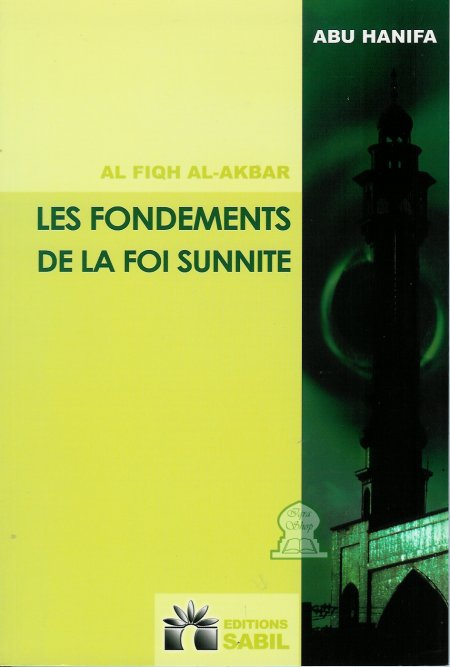
\includegraphics[width=3cm]{Images/image075.jpg}}



{On en trouve sa traduction et son
commentaire en français.
}

Elle témoigne de l'émergence de nouvelles questions.

Par exemple, si vous prenez le premier article~: il y est dit que la foi
consiste à témoigner par la langue, l'assentiment du cœur et l'esprit~:
il ne suffit donc pas de dire, il faut croire à ce que l'on dit et aussi
comprendre ce que l'on dit. Certains diront que l'assentiment du cœur
suffit, et qu'il n'est pas nécessaire de prononcer la
\emph{šahāda}\ldots{} D'autres diront que le dire suffit aux yeux des
hommes, mais non aux yeux de Dieu\ldots{} Bref, ces professions de foi
sont les conséquences de questions théologiques.

De même, il est dit que la foi ne peut pas croître ou décroître. On a la
foi ou on ne l'a pas. Ce ne sera pas l'avis des \textbf{ašʿarites}.

Dans l'article 2, il est dit qu'un musulman qui commet un péché demeure
toujours musulman. Ici, l'article s'oppose explicitement aux
\emph{ḫariǧites} qui affirment le contraire et qui prônent un islam
d'une moralité très rigoureuse.

La \emph{Waṣiyya} se prononce aussi sur le caractère incréé du Coran
(art. 5) et donne des précisions sur l'eschatologie.

Les discussions se précisent toujours davantage et l'on voit aborder
toutes les grandes questions théologiques~: problème de la foi, du
\emph{tawḥīd}, du Coran, de la prédestination, de la prophétologie, de
l'eschatologie, du culte et du califat.






\subsection{Pour aller plus loin}

Daniel \textsc{Gimaret}, \emph{La doctrine d'al-Ash`arî}, Paris, Cerf,
Collection Patrimoine Islam, 1990.

C'est un excellent livre, mais il est très difficile, très technique.
Bref, pour les plus courageux, et surtout pour ceux que ces questions
passionnent.
 
  %8
\include{IbnToumart}
\chapter{Le šī`isme ou l'islam sous un autre visage}

Avant d'exposer les doctrines et pratiques propres au šī`isme, je vous
propose de regarder cette petite vidéo d'un peu moins de 10 minutes.
Elle sera une bonne introduction de ce qui est dit du šī`isme. Vous
devrez pouvoir répondre aux questions de l'encadré ci-dessous. Pour
autant si ce cours va permettre de préciser les informations
mentionnées, il en révélera aussi quelques dimensions que ne signerait
pas un šī`ite. C'est tout le problème de l'imbrication entre la
théologie et l'histoire.

\paragraph{Questions}

\begin{enumerate}
\def\labelenumi{\arabic{enumi}.}
\item
  D'où vient le mot šī`ite~?
\item
  Quel est l'évènement fondateur du šī`isme~?
\item
  Quelles sont les principales villes saintes du šī`isme~?
\item
  Le šī`isme est-il un phénomène spécifiquement persan~?
\end{enumerate}


En raison de la révolution iranienne en Iran en 1979, l'image du šī`isme
véhiculée en Occident a été bien souvent celle de croyances
obscurantistes, d'intolérance, de régression, de violence politique. En
2004, Mohammad Amir-Moezzi et Christian Jambet pouvaient écrire~dans un
ouvrage de grande qualité pédagogique, \emph{Qu'est-ce que le
shî'ism~?}~: «~le shî'isme est une figure de style pour `islam radical',
voire pour `islam terroriste'~»\sn{Mohammad-Ali
  \textsc{Amir-Moezzi}, Christian Jambet, \emph{Qu'est-ce que le
  shî'isme~?,} Paris, Fayard, 2004.} (p. 12).

Cette image est en train de disparaître. Le départ de la scène politique
du président Mahmoud Ahmadinejad après deux mandats (2005-2013) et le
climat de détente avec les États-Unis y est sans doute pour beaucoup.
Sans compter, bien sûr, Al-Qaida, Daesh, autant d'émanations d'un islam
politique extrémiste instrumentalisant le meurtre et la terreur, qui ne
sont pas šī`ites mais sunnites. J'ajouterai que le travail de
vulgarisation des islamologues sur le šī`isme, d'historicisation, de
contextualisation de la République islamique d'Iran et de l'idéologie de
l'ayatollah Khomeiny par rapport à ce courant musulman qui prend son
origine au premier siècle de l'islam y a aussi sa part. Le cinéma
contribue aussi à donner une autre image de la société iranienne.

Mais fondamentalement, qu'est-ce que le \emph{šī`isme}~? S'agit-il d'un
autre islam que le sunnisme ou du même islam mais avec un visage
différent~? Les oppositions politiques au cours de l'histoire, les
polémiques virulentes notamment durant la période des empires ottomans
et safavides, donnent l'image de deux irréductibles, de deux
irréconciliables, de deux frères ennemis. Avoir conscience et
connaissance de la singularité du \emph{šī`isme} ne doit pas faire pour
autant oublier que les šī`ites se disent musulmans et qu'il existe des
penseurs travaillant pour un «~œcuménisme~» entre sunnisme et šī`isme.
Telle est l'approche par exemple de Seyyed Hossein Nasr qui présente le
šī`isme comme «~une affirmation d'une dimension particulière de l'islam
qui est centrale et qui est considérée par les \emph{šī`ites} comme
faisant partie de l'islam en tant que tel. Il n'a pas été un mouvement
qui a d'une certaine manière détruit l'unité de l'islam, mais un de ceux
qui a ajouté à la richesse du déploiement historique et de la diffusion
du message coranique~»\sn{Seyyed Hossein Nasr dans Sayyid Muḥammad
  Husayn Ṭabāṭabā'ī, \emph{Shi‛ite Islam} , translated and edited by
  Seyyed Hossein Nasr , Albany, State University of New York Press,
  1975, p.7.}.

Certes, il existe des aspects historiques et religieux du šī`isme qui
contredisent le sunnisme, mais ce professeur iranien de philosophie
appelle à y voir le signe d'une pluralité d'interprétations possibles.
Il ne s'agit pas d'élaborer un dénominateur commun mais de voir que
l'unité embrasse les différentes «~facettes de l'islam~». Pour lui,
c'est dans la mystique, la spiritualité, l'ésotérisme qu'il est possible
de transcender, de dépasser les différences et de trouver l'unité. 


Mais avant de voir comment sunnisme et šī`isme relèvent tous deux de la
même unité qu'est l'umma, la communauté musulmane, quels sont les
éléments fondamentaux d'histoire, de doctrines et de pratique du
šī`isme~?


\section{Les fondations du šī`isme~: histoire
}
\subsection{Origine du šī`isme~: la
question de la
succession}


Le terme arabe \emph{šī`a} signifie
parti, adhérent, fidèle. S'il y est mentionné que l'acte de naissance du
šī`isme est la bataille de Kerbala\sn{
Kerbala~: c'est la ville qui n'a pas défendu les enfants du prophète.
Rédemption par le sang.}
, pour les šī`ites, le šī`isme
existait du vivant de Muḥammad.

`Alī en effet est le fils d'Abū Ṭālib, l'oncle paternel de Muḥammad. Il
est un des premiers convertis à l'islam. La tradition sunnite mentionne
que le Prophète lui avait confié (amāna) les biens des personnes dont il
était le représentant commercial et financier peu avant l'Hégire, que le
soir de l'Hégire, lorsqu'il quitta La Mecque, `Alī dormit dans son lit,
qu'il épousa Fāṭima, l'une des filles du Prophète.

Fāṭima joue un rôle très important dans l'histoire du šī`isme. Elle
décède à l'âge de 28 ans et `Alī n'épousera aucune autre femme. Il
semble, d'après les traditions šī`ites que Muḥammad avait imposé à son
gendre la monogamie pour sa fille Fāṭima. Elle aurait aussi obtenu de
son père l'autorisation d'aller prier sur les tombes de ceux qui avaient
été tués au cours des batailles.

À la mort du Prophète s'est posée la question de savoir qui allait
succéder à Muḥammad. Pour `Alī et ses partisans, Muḥammad a désigné son
successeur de son vivant. En effet, peu de temps avant sa mort, en 632,
Muḥammad se rendit à \emph{Ġadir Ḫumm~}: c'est le pèlerinage d'adieu (Ḥaǧǧa
al-widā').
\begin{marginfigure}
    \centering
    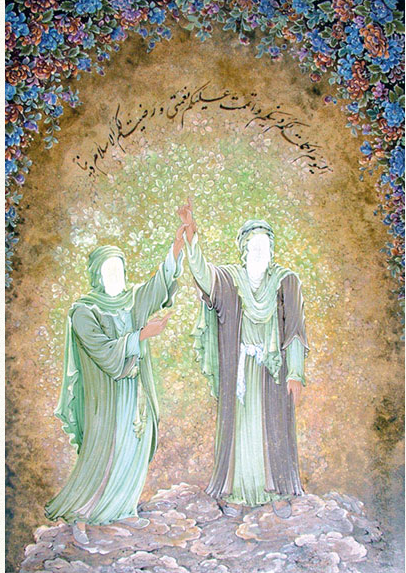
\includegraphics[width=1.35188in,height=1.90972in]{Images/image078.png}
    \caption{Ġadir-e Khumm et la
désignation de l'Imâm `Alī. œuvre de Rezâ
Badr-os-Samâ'}
    \label{Ġadir-e Khumm}
\end{marginfigure}

Il y reçut le verset suivant~: 
\begin{quote}
  {«~O Messager, transmets
ce qui t'a été descendu de la part de ton Seigneur. Si tu ne le faisais
pas, alors tu n'aurais pas communiqué Son message. Et Dieu te protégera
des gens. Certes, Dieu ne guide pas les gens mécréants.~» (Coran,
5:67).}  
\end{quote}


Par la suite, selon les šī`ites, Muḥammad déclara~: «~Man kuntu Mawlāhu,
fahaza `Alī mawlāhu~» c'est-à-dire~: «~Qui me reconnaît comme son Mawlā
(maître, guide), doit reconnaître `Ali comme son Mawlā ~».




Mais pour certains des compagnons du Prophète, cette désignation n'a
jamais été officialisée et selon les mœurs tribales, il convient donc de
procéder à son élection.

Mais `Alī est écarté du collège électoral. \mn{\cite{OUARDI:CalifesMaudits}} 

La tribu des Qurayš élit Abū Bakr, vieux compagnon et un des beaux-pères
de Muhammad~: il devint le 1\textsuperscript{er} calife (khalîfa).

`Alī fera acte d'allégeance, il se soumet à ce choix signifiant son
désir de maintenir l'unité de l'\emph{umma}.

À la mort d'Abū Bakr, `Umar devient le 2\textsuperscript{ème} calife
puisqu'il avait été désigné de manière explicite (\emph{naṣṣ}). `Alī
accepte.

`Umar annonce qu'à sa mort, son successeur devra être choisi parmi les
membres d'un collège électoral qu'il a lui-même nommés. `Alī en fait
partie. À la mort de `Umar, c'est `Uṯmān qui est choisi. Accusé de
népotisme, il est assassiné.

`Alī devient alors le 4\textsuperscript{ème} calife (656-661) attestant
ainsi de ses qualités vertueuses et de la suprématie de l'imamat sur les
manigances politiques mondaines.

Pour autant, deux anciens compagnons du Prophète n'ayant pas vu leur
appétit politique satisfait -- ils souhaitaient être gouverneurs de Kūfa
et Baṣra -- s'associèrent à `Ā'iša, fille d'Abū Bakr et veuve du
Prophète, pour lever une armée contre `Alī. C'est la bataille du chameau
de 657. On l'appelle ainsi parce que `Ā'iša qui était présente, était
montée sur un chameau\ldots{} Son armée fut mise en défaite.





\mn{On voit ici `Ā'iša sur son chameau et dans son baldaquin}



Mais en Syrie, Mu`āwiya, parent de `Uṯmān, mena aussi une guerre. C'est
la bataille de Ṣiffīn. Alors qu'elle tournait à l'avantage de `Alī,
Mu`āwiya proposa un arbitrage sur le livre sacré. `Alī accepte. Nombre
de ses soldats se soulèvent considérant qu'il n'avait pas à accepter
l'arbitrage et que Dieu avait déjà rendu son jugement par la victoire
qui se manifestait. `Alī doit mener combat contre ces rebelles (ce sont
les ḫariǧites), alors que Mu`āwiya se fait proclamer calife à Jérusalem
en 660~!

`Alī est assassiné par un ḫarigite à Kūfa en 661.

Pour les sunnites, il n'avait pas de successeur tandis que les šī`ites
affirment qu'il avait nommé son fils aîné, al-Ḥasān.

 
\subsection{La généalogie du
šī`isme}\label{la-guxe9nuxe9alogie-du-ux161ux12bisme}

La généalogie est sujet à controverses et divergences ce qui explique la
multiplication des šī`ismes\textbf{.} On dénombre une centaine de
lignées à la fin du premier siècle de l'Hégire.

Les jours de naissances des membres de la famille de `Alī sont des fêtes
religieuses. Les jours anniversaires de leur mort, des journées de
deuil. Leurs tombes sont des lieux de pèlerinage~: les cités où elles se
trouvent sont des villes saintes.

Elle est un peu subtile, chaque imām mériterait un chapitre\ldots{}
entre son enseignement, les histoires, les légendes, leur assassinat --
souvent empoisonné -- sans compter qu'au sein même du šī`isme, les
généalogies, les filiations ne sont pas les mêmes, que certains ne
reconnaissent que quatre imāms, d'autres sept, d'autres douze, que ce ne
sont pas toujours les mêmes\ldots{} qu'il y a donc une multitude de
branches šī`ites\ldots{} Bref, je retiens surtout le šī`isme majoritaire
dit duodécimain, car il reconnaît 12 imāms. Vous en trouverez en annexe
la liste avec leurs noms et quelques caractéristiques. Si vous avez la
curiosité de regarder le douzième, vous voyez que n'est pas indiquée la
date de sa mort. D'après vous, est-ce parce que l'on ne la connaît pas,
ou est-ce pour une autre raison~? La réponse dans la suite du cours. Bon
travail.

 
\paragraph{`Alī et Fātima}\label{alux12b-et-fux101tima}

`Alī joue donc dans le šī`isme un rôle important. Il est à la tête de
presque toutes les chaînes de transmission, il est considéré ~comme un
maître spirituel. On lui attribue deux livres~: \emph{Nahj al-balâgha}
(La Voie de la maturité)~et \emph{Dîwân}, un recueil de poèmes.

Quant à Fātima, elle est la sainte la plus vénérée du šī`isme\textbf{.}
Sa tombe est à Médine (il y en a trois\ldots{} dans le doute, on les
garde toutes les trois).

Fātima est la mère de toute la lignée des imāms. Elle représente ce qui
relie Muhammad à `Ali, la lettre et l'esprit. Elle est dite \emph{maǧma`
al-nūrayn} (le Confluent des Deux Lumières), celle de la prophétie et de
l'imamat. Elle a une mission d'intercession et de protection jusqu'à la
fin des temps. Immaculée, Vierge malgré son mariage, elle est aussi
reine du ciel. Un parallèle avec Mariam (Marie), la mère de Jésus est
établi par la tradition šī`ite elle-même \sn{Tahani Sabri,
  «~L'hagiographie de Fāṭima d'après le \emph{biḥār al-anwār}~», École
  des Hautes Études en Sciences Sociales, thèse de doctorat sous la
  direction de Henry Corbin, 1969.}.

 
\paragraph{Al-Hasan, fils de
`Alî}\label{al-hasan-fils-de-aluxee}

C'est un petit-fils du Prophète. Il y a des récits touchant d'affection
tendre.

Al-Ḥasan abdiqua le califat devant l'hostilité de Mu`āwiya. Pour les
historiens šī`ites, il préféra l'unité de la communauté plutôt que de
voir la division, mais les sunnites font remarquer qu'il n'était pas en
mesure de remporter la victoire et qu'il abdiqua en contre-partie d'une
importante somme d'argent. Retiré à Médine, il est assassiné,
semble-t-il par une de ses épouses qui aurait été soudoyée, selon les
šī`ites par Mu`āwiya. Terrible Mu`āwiya\ldots{} J'imagine que vous ne
devez pas le trouver très sympathique. Il est le fondateur de la
dynastie Omeyyade. Les grands historiens sunnites des
8\textsuperscript{ème} et 9\textsuperscript{ème} siècles n'en ont pas
laissé un souvenir très élogieux\ldots{} car ils sont abbassides et il
fallait effacer les traces vénérables des Omeyyades.

 
\paragraph{Al-Ḥusayn} 

Al-Ḥusayn, le second fils de `Alī, reste discret. Il s'efface. Mais il
entre sur la scène politique au moment de la mise en place d'une
dynastie califale héréditaire en la personne de Yazīd, le fils de
Mu`āwiya. On se réfère souvent à lui pour présenter le šī`isme comme un
courant révolutionnaire, politique et contestataire.

L'histoire est plus complexe. En tous les cas, les sources appellent une
très grande prudence. Assuré du soutien de la ville de Kūfa, il se met
en route avec toute sa famille pour chasser les Omeyyades. Mais sur la
route, la petite troupe se trouve encerclée par les soldats omeyyades,
coupée de Kūfa, privée d'eau. Retranchée en plein désert dans un petit
village appelé Karbalā', les Omeyyades finissent par donner l'assaut.
C'est un massacre. Ḥusayn est tué, décapité, piétiné ainsi que quasiment
toute sa famille.

Ašura est le jour de célébration où l'on fait mémoire de cette tragédie
dans de grandes cérémonies populaires avec parfois des dérives
spectaculaires de lamentations violentes, d'auto-flagellations, de
lacérations ou de mutilations. C'est le remord d'une ville qui n'a pas
soutenu al-Ḥusayn.

Ḥusayn devint alors un exemple de martyr, de sacrifice, de bravoure.
Sans-doute, sous l'influence chrétienne, on verra dans la mort de Husayn
un sacrifice rédempteur pour le salut des fidèles.

Chez certains fidèles la rumeur selon laquelle il ne serait pas mort
circule. Il aura été enlevé au ciel directement par Dieu avant le
combat.


\mn{Les troupes omeyyades encerclent Karbalā' \& Yā Ḥusayn\ldots{}

Jour de la fête d'Ashura \& Ashura et ses spectaculaires flagellations à
Karbalā'\ldots{} }


 
\paragraph{`Alî Zayn al-`Âbidîn, fils
d'al-Husayn}\label{aluxee-zayn-al-uxe2biduxeen-fils-dal-husayn}

Un rescapé du massacre de Karbalâ'. Il serait parti à Médine pour y
mener une vie pieuse. Il ne posa aucun problème aux Omeyyades. Une
existence ascétique, consacrée à la dévotion. On le surnommait
\emph{al-saǧǧād}, celui qui accomplit de nombreuses prosternations.
C'est un nom respecté, même dans le sunnisme.

Un de ses fils Zayd ibn `Alî, est à l'origine d'une grande famille, les
zaydites. Le zaydisme est marqué par un activisme violent. Selon la
théorie zaydite de l'imamat chaque Alide a le droit de prétendre à la
direction de la communauté. Le véritable imâm est celui qui se qualifie,
les armes à la main, en s'insurgeant contre le pouvoir injuste. Ils sont
aujourd'hui encore influents au Yémen~où ils représentent la moitié de
la population (mais le dernier chef zaydite du Yémen a été renversé en
1962).

 
\paragraph{Muhammad al-Bāqir, fils de `Alî Zayn
al-`Âbidîn}\label{muhammad-al-bux101qir-fils-de-aluxee-zayn-al-uxe2biduxeen}

Il est considéré comme le fils de `Ali Zayn. Les grandes traditions
šī`ites le considèrent comme le 5ème Imām. Il est surnommé Abū Ǧa`far.

 
\paragraph{Ǧa'far al- Ṣādiq
}\label{ux1e7afar-al--ux1e63ux101diq}

Fils de Muhammad al-Bāqir, il est célèbre pour sa piété et, selon les
shiites, l'infaillibilité de ses prémonitions. Les auteurs soufis lui
attribuent le plus ancien commentaire mystique du Coran. On le considère
comme un alchimiste, un spirituel refusant toute implication dans les
mouvements politiques de son époque. Il fut enterré dans le cimetière de
Baqī` à Médine. Le carré šī`ite y sera rasé au XIX° siècle par les
Wahhabites, alors qu'il abritait les tombes de plusieurs imâms.

Son fils aîné, Ismā`īl, est l'éponyme de la seconde grande famille de
l'islam šī`ite, les ismaéliens, šī`ites septimains \textbf{--} shî'ites
à 7 imâms. Pour cette branche, il est le dernier Imâm. Un autre groupe
s'appuie sur la croyance que l'imamāt fut transmis du vivant de Ǧa`far à
son petit-fils~: ce sont les qarmates. D'autres, les Fatimides,
considèrent que l'imamat se poursuit et que l'imam caché, le Mahdi, sera
un de ses descendants.


\begin{Synthesis}
Le si'isme est  une prophétologie. Il y a une sur
l'incarnation. Facilite le
dialogue avec les chrétiens.
\end{Synthesis}

 
\paragraph{{Le douzième imām, l'imām caché ou
le Madhī
}{ }}\label{le-douziuxe8me-imux101m-limux101m-cachuxe9-ou-le-madhux12b}

À la mort du 11\textsuperscript{ème} imâm, les fidèles croient que
l'imâm a eu un fils du nom de Muḥammad. 
\begin{Def}[Mahdî]
Il est reconnu comme le
\emph{Mahdî,} le Bien Guidé. C'est l'imâm caché, \emph{al-imâm al-ġā'ib}
ou encore \emph{al-Qā'im}, que l'on peut traduire par le Résurrecteur.
\end{Def}


C'est le courant duodécimain, majoritaire dans le šī`isme.

Mais en quoi consiste cette occultation~? Comment s'opère-t-elle~? Que
signifie-t-elle~? Quand a-t-elle eu lieu~? Sous quelles formes~?

Je vous propose d'écouter ce bref passage d'une émission sur France
Culture, «~Les racines du ciel~», où Amir-Moezzi répond.

L'imâm caché n'est donc pas mort. Vous comprenez maintenant pourquoi
dans le tableau en annexe ne figure que sa date de naissance. Il
n'existe pas de successeur puisqu'il est physiquement vivant. À la fin
des temps, il se manifestera. Il y a donc une présence invisible, mais
physiquement réelle. L'imâm caché clôt la lignée des imamites.

Par la suite, tout se passe comme si désormais l'ère de la bonne entente
entre le religieux et le politique était désormais finie. La cité
idéale, gouvernée par un juste n'est réalisable qu'à la fin des temps,
avec l'avènement du Mādhi, le Sauveur eschatologique. L'attitude
revendicative et politique est rejetée dans un futur messianique. Le
šī`isme se présente comme une religion individuelle, personnelle, non
institutionnelle. Mais peut-il alors perdurer ? Pour pallier cette
«~absence~», on aura recours à la figure du juriste avec la dynastie
bouyide. C'est à cette époque que le šī`isme sera érigé comme religion
d'État, ce qui n'est pas le moindre des paradoxes compte tenu de ses
«~fondamentaux~».

 
\section{Les fondations du šī`isme~:
doctrines}\label{ii.-les-fondations-du-ux161ux12bisme-doctrines}

Les doctrines šī`ites sont compliquées, subtiles et à lire
l'enseignement des imāms et les commentaires qui en suivirent, cette
subtilité est voulue pour elle-même. De leurs enseignements, ils ne
cessent de dire~: «~notre enseignement est ardu, difficile à supporter~:
c'est un secret, un secret enveloppé par un secret au sujet d'un
secret~»\sn{Voir Amir-Moezzi, Jambet, \emph{Qu'est-ce que le
  shi'isme~?}, Paris, Fayard, p. 96 .}.

Dans sa présentation du šī`isme, Amir-Moezzi distingue dans la vision du
monde et la théologie šī`ite une double dimension~: elles sont marquées
à la fois par l'affirmation d'un principe de dualité et d'un principe de
dualisme. On lira avec intérêt et pour plus de précisions la
présentation qu'il fait dans \emph{Qu'est-ce que le shiisme~?} Mais tout
d'abord, la question des Écritures. Sont-elles les mêmes qu'en
sunnisme~?

 
\subsection{{Les sources scripturaires
}}\label{les-sources-scripturaires}

 
\paragraph{{Y a-t-il un Coran šī`ite~?
}}\label{y-a-t-il-un-coran-ux161ux12bite}

Le Coran est la référence principale et la contradiction éventuelle
entre un \emph{ḥadīṯ} et un verset coranique est l'indice de la fausseté
du ḥadīṯ.

Pour autant, certaines traditions shî'ites trouvent difficilement leur
fondement dans le Coran. Pour les šī`ites, le Coran a été en réalité
falsifié, altéré, censuré lors de sa compilation par `Uṯmān (c'est un
des premiers califes. Si le nom ne vous disait plus rien du tout,
revoyez le premier cours sur le Coran et à la question du
\emph{muṣhaf}). La révélation originelle contenait des versets sur `Alî
et les descendants des Prophètes. Ils étaient cités comme les modèles et
les chefs par excellence. `Alī possédait une version du Coran intégral,
mais il n'en dit mot pour éviter sa destruction par ses adversaires.
Cependant, elle fut transmise secrètement d'imam à imam, jusqu'au
12\textsuperscript{ème} imâm qu'il l'emporta avec lui lors de son
Occultation. Les enseignements des imāms permettent d'accéder à ces
versets et de les connaître.

Avec l'arrivée au pouvoir des Bouyides shiites à la fin du
4\textsuperscript{ème} siècle de l'hégire, il s'agira de trouver un
accord avec l'orthodoxie sunnite. On met ainsi un terme au doute sur
l'intégrité du Coran officiel. Le courant dominant abandonne la thèse de
la falsification du Coran officiel, mais le débat ressurgit
régulièrement.

 
\paragraph{Y a-t-il un \emph{ḥadīṯ} šī`ite~?
} 

Bien qu'al-Būḫārī fut perse, il existe une Sunna šī`ite. Les textes sont
bien souvent les mêmes, mais les \emph{isnāds} diffèrent et renvoient
aux membres de la famille du prophète (\emph{ahl al-bayt} --
c'est-à-dire littéralement, les gens de la maison). En effet, la
référence dans l'\emph{isnād} aux compagnons du Prophète lui ôte toute
crédibilité dans la mesure où ils sont considérés comme des traîtres.
Pour l'\emph{isnād}, la notion a été vue dans le cours sur la Sunna.
C'est la fameuse chaîne de transmission.

On reconnaît trois grands corpus~:

\begin{itemize}
\item
  Celui de Ya`qub al-Kulaynī (m. en 939).
\item
  Celui de Saduq Ibn Babuyeh (m. 991).
\item
  Celui d'al-Ḥasan al-Tusī (m. 1068).
\end{itemize}

On trouve aussi dans ces recueils de nombreux témoignages des imāms.

L'ouvrage le plus connu de Kulaynī est \emph{al-Kāfī}. Il est divisé en
trois sections~:

\begin{itemize}
\item
  \emph{Usūl al-Kāfī}, qui concerne l'épistémologie, la théologie, la
  question de la foi et de la mécréance, l'histoire, l'éthique, et le
  Coran~et ses mérites;
\item
  \emph{Furūʿ al-Kāfī}, qui concerne les dimensions pratiques et légales
  (prières, \emph{ǧihād}, jeûne, ḥaǧǧ, funérailles, nourriture, boisson,
  mariage, divorce, commerce, héritage, etc.)
\item
  \emph{Rawdat} \emph{al-Kāfī}, qui inclue de nombreuses traditions, des
  lettres, des discours des imāms.
\end{itemize}

Il existe une traduction anglaise de cette collection de plus de 16 000
traditions. Si vous ne trouvez pas le sommeil\ldots{}
 
\subsection{ Dualité et dualisme}\label{dualituxe9-et-dualisme}

 
\paragraph{ Une vision duelle}\label{une-vision-duelle}

Il s'agit d'affirmer que toute réalité possède deux niveaux~:

1/ un niveau manifeste, obvie, apparent, visible, concret, évident
(\emph{zāhir})

2/ un niveau secret, non manifeste, implicite, invisible, intérieur
(\emph{bāṭin})

Cette affirmation est au cœur du credo šī`ite. Ce que je vois, ce qui
est visible contient aussi une réalité invisible. Il existe une relation
entre le manifeste et le caché, l'exotérique et l'ésotérique. Il s'agit
d'appliquer ce principe à toute réalité, et bien sûr, à commencer par la
théologie.

\emph{Ainsi, en théologie}, Dieu a deux niveaux d'être, deux niveaux
ontologiques~:

1/ son Essence, inconcevable, inimaginable, au-delà de toute pensée~:
c'est le niveau caché (\emph{bāṭin})

2/ ses Noms et Attributs~à travers lesquels Dieu se révèle et se fait
connaître~: c'est le Dieu inconnu qui aspire à être connu. Amir-Moezzi
remarque que l'on retrouve une distinction de la théologie médiévale
chrétienne entre \emph{Deus absconditus} et \emph{Deus revelatus}.

La manifestation de ces noms divins comme le Roi, le Miséricordieux, le
Juge suprême, etc. est une manifestation de Dieu (théophanie). La plus
haute révélation en est la figure de l\emph{'Imām} céleste,
l'\emph{Imām} de Lumière, l'Homme cosmique~: c'est l'Imām avec un I
majuscule, dans son acception ontologique universelle.

L'\emph{Imām} cosmique a aussi deux dimensions

\begin{quote}
1/ la dimension cachée~: c'est l'aspect métaphysique, dans le ciel,
invisible à nos yeux.

2/ la dimension exotérique, visible~: ce sont les \emph{imāms}
historiques.
\end{quote}

La mission de ces \emph{imāms} historiques~consiste à dévoiler les
mystères de Dieu, du monde et de l'homme, à transmettre aux hommes le
Secret contenu dans l'Imām métaphysique.

Mais l'enseignement des imāms, disions-nous, est complexe. Ǧa`far
al-Ṣādiq (c'est un \emph{imām} que nous avons rencontré dans la
généaologie des douze\ldots{} C'est le combientième \emph{imām} déjà~?)
écrivait~: «~Notre enseignement comporte l'exotérique, l'ésotérique et
l'ésotérique de l'ésotérique~».

À cette approche duelle de la réalité se superpose le principe du
dualisme.

 
\paragraph{ Une vision dualiste}\label{une-vision-dualiste}
\mn{Si isme~: influence de la zoroastrisme avec un certain manichéisme, bien
/ mal. Lumière et nuit~; combat cosmique et sur terre. On retrouve ceci
dans le sunnisme. Tous les Hadiths eschatologiques décrivent en tableau
le paradis. Dans le Si isme, enjeu du bien et du mal.
}
L'histoire de la création est celle d'un combat cosmique entre les
forces du Bien et les forces du Mal, entre la lumière et l'obscurité. On
retrouve ici une nette dimension zoroastrienne et manichéenne du monde.

Ce combat se situe au niveau cosmique~: c'est le combat entre les armées
de l'Intelligence cosmique (\emph{al-`aql}) et celles de l'Ignorance
cosmique (\emph{al-ğahl}). Cette dichotomie, cette opposition est celle
d'une lutte permanente entre les Gens de la Droite (\emph{ašāb
al-yamīn}) et les gens de la Gauche (\emph{ašāb al-šimāl}). Le combat
entre deux hommes ennemis s'inscrit donc dans un cadre plus large. Toute
l'histoire de l'humanité est traversée par l'adversité et la violence
des forces démoniaques de l'Ignorance. Il en sera ainsi jusqu'à la fin
des temps avec l'avènement du Sauveur eschatologique, le Mahdī qui
vaincra définitivement les forces du mal.

Mais qui sont ces forces du mal~? Comment les reconnaître, les
identifier~?

C'est l'enseignement des imāms (les 7, les 12, selon) qui apportent les
réponses à ces questions. Dans ce corpus de centaines de milliers de
pages, les adversaires de l'imâm~sont tour à tour identifiés~:

\begin{itemize}
\item
  Aux juifs, qui sont des idolâtres et ont trahi Moïse en adorant le
  veau d'or
\item
  Aux Compagnons de Muhammad qui ont rejeté `Alī
\item
  Aux Gens de l'exotérique, c'est-à-dire des apparences, du superficiel
  (\emph{ahl al-zāhir}), ce sont les littéralistes qui s'arrêtent à la
  lettre et n'ont pas connaissance de son `esprit' (\emph{bāṭin}). À cet
  égard, un šī`ite se sentira plus proche d'un juif ou d'un chrétien
  accoutumé à une lecture ésotérique, symbolique, anagogique des textes
  que d'un musulman sunnite exotérique, qui se limite à la lettre.
\end{itemize}

 
\subsection{Prophétie et
Imamologie}\label{prophuxe9tie-et-imamologie}

L'enseignement des \emph{imāms}, acquiert en réalité un rôle supérieur à
celui du Prophète.

En effet, si le prophète est le messager de la lettre, l'\emph{imām}
dans le šī`isme en apporte l'esprit. Or, si l'esprit peut exister sans
la lettre, sans l'esprit, la lettre est morte\sn{Amir-Moezzi,
  Jambet, \emph{Qu'est-ce que le shi'isme~?}, Paris, Fayard, 2004, p.
  42.}.


\paragraph{Remarque sur l'imām~}: le mot \emph{imām}
est piégé. Il s'emploie en sunnisme, mais sans désignation particulière.
L'imām désigne un savant, un chef ou tout simplement celui qui dirige la
prière. En revanche, en šī`isme\textbf{,} c'est un titre sacré. L'imām
est le Guide, l'un des Douze\ldots{} En principe, aucun autre homme ne
porte ce nom. Et pourtant, d'aucuns se sont attribués ce titre. Autant
dire qu'ils se prenaient pour le Mahdi .L'un d'eux est très célèbre. À
suivre.

L'Imām apporte en effet la connaissance face au monde de l'ignorance. En
montrant son cœur, l'Imām `Alī donnait cet enseignement sur la vocation
de l'imām, la nature de la religion, son importance. Écoutez et
réécoutez ce texte\sn{Vous trouvez l'intégralité du texte dans le
  livre de Mohammad Ali Amir-Moezzi, \emph{La religion discrète}, Paris,
  Vrin, 2006,
  \url{https://books.google.com}}.


L'imām transmet les vérités secrètes. Il tient le monde, il évite la
noyade définitive du monde dans les ténèbres. Il est l'alpha et l'omega
du šī`isme\sn{Amir-Moeezi, Jambet, \emph{Qu'est-ce que le
  shi'isme~?}, p. 40.}.

Mais il a aussi des pouvoirs supra-normaux~: il possède la science du
passé et du futur, il lit dans les consciences, il connaît les langues,
y compris celle des animaux, les sciences occultes (astrologie,
alchimie, sciences divinatoires, etc.). Il peut ressusciter les morts,
guérir les maladies, rajeunir les vieillards, marcher sur les eaux,
monter aux cieux\ldots{} Il possède des objets de pouvoir~ tels la
tunique d'Adam, le sceau de Salomon, l'Arche et les tables de la Loi,
l'Arme invincible de Muḥammad.

L'enseignement de l'\emph{imām} est au cœur de l'approche spirituelle
šī`ite. C'est par lui que se réalise la spiritualisation, la
divinisation. Écoutez Amir-Moezzi à ce sujet.

 
\subsection{La walāya au cœur de la foi šī`ite
} 


La \emph{walāya} est un concept clé du \emph{šī`isme}. Les
\emph{šī`ites} sont appelés les gens de la \emph{walāya}.\\
\begin{Def}[walāya]
La \emph{walāya} désigne la mission sacrée et sainte des imams.

L'imām est le \emph{walī} (le saint), celui qui initie les fidèles à
l'esprit de la Parole divine. Il est la Face de Dieu sur terre.

\end{Def}



La \emph{walāya} désigne aussi l'amour, celui que les fidèles
manifestent dans la dévotion, par la loyauté, la soumission à l'égard du
maître initiateur.

Mais dans une doctrine \textbf{dualiste}, l'amour de l'imām ne peut aller sans la
haine de son ennemi. La \emph{walāya} est donc inséparable de son
contraire, la \emph{barā'a} (c'est-à-dire la haine, la dissociation à
l'égard des forces de l'ignorance). Un \emph{ḥadīṯ} šī`ite dit~:

\begin{quote}
«~l'amour de Dieu ne s'obtient que grâce à l'amour envers Ses amis et
l'hostilité à l'égard de Ses ennemis~».    
\end{quote}


Au cœur de la foi šī`ite, la \emph{walâya} est dans la \emph{šahāda} :
\begin{quote}
   «~Je témoigne qu'il n'y a pas de dieu hormis Dieu~; je témoigne que
Muhammad est l'envoyé de Dieu, et que `Alî est le \emph{walī} de
Dieu~» 
\end{quote}
 \emph{walī} signifie ici l'ami,~l'allié, le détenteur de la
\emph{walāya}.




\mn{\emph{Šahāda} sur une mosquée du Caire
fatimide. on y lit à la fin~:\emph{ʿAlī walī
allāh.
}  }


\subsection{{Les signes de la fin du monde ou
l'eschatologie šī`ite
}\label{les-signes-de-la-fin-du-monde-ou-leschatologie-ux161ux12bite}}

En raison de la place de la question de l'Occultation, l'eschatologie a
donné lieu à un foisonnement de traditions et de traités. Il s'agit de
savoir lire les signes afin de reconnaître l'imminence du Dernier Jour,
le retour du Mahdī. Les signes sont multiples, mais on peut identifier
quelques constantes~:

\begin{itemize}
\item
  l'envahissement de la terre par les forces du Mal,
\item
  l'écrasement quasi-complet des forces de la Connaissance par celles de
  l'ignorance,
\item
  la perte du sens du sacré,
\item
  le renversement des valeurs humaines,
\item
  l'anéantissement de tout ce qui relie l'homme à Dieu et à son prochain
\end{itemize}

Des signes concrets sont exposés. Ainsi par exemple,

\begin{itemize}
\item
  la venue d'al-Sufyānī, le chef de l'armée des ennemis des imāms, le
  collaborateur d'\emph{al-Daǧǧāl}, l'Imposteur, l'Antéchrist islamique.
\item
  L'avènement d'al-Yamānī, le Yéménite qui prêchera le soutien au Mahdī.
\item
  Le Cri, d'origine surnaturelle, venu du ciel, appelant les hommes à
  rejoindre l'armée du Sauveur
\item
  L'engloutissement d'une armée (parfois celle d'al-Sufyānī) dans le
  désert.
\item
  L'assassinat à La Mecque de l'envoyé du Mahdī, appelé \emph{al-Nafs
  al-Zakiyya\textbf{~}}: l'Âme Pure.
\end{itemize}

La fin de l'occultation est aussi expliquée et commentée. On peut en
distinguer 3 raisons~principales :
\begin{enumerate}
    \item une raison historique~: venger tous les hommes saints du passé,
victimes de l'injustice. Tous les saints du passé reviendront à la vie,
ainsi que leurs meurtriers, et les premiers pourront ainsi se venger des
seconds à cette occasion.
\item une raison religieuse~: rétablir le sens du sacré~; rétablir les
religions (judaïsme, christianisme, islam) dans leur intégralité
originelle, rapporter les Écritures respectives qui ont été altérées ou
falsifiées
\item une raison spirituelle~: apporter le sens ésotérique des choses,
effacer la frontière entre le caché et le manifeste.
\end{enumerate}
 

Le retour du Mahdi s'accompagne aussi de celui de Jésus-Christ. Il est
le principal compagnon d'al-Qā'im. Voyez un peu plus haut. C'est un nom
utilisé pour nommer le Mahdi. Quelle est sa signification déjà~? Penser
à «~\emph{Talitha Qum~}».. Lève-toi\ldots{} C'est bien la même racine du
redressement, de la résurrection.

 
\section{Bibliographie}\label{bibliographie}

\paragraph{Les fondamentaux}

Mohammad-Ali \textsc{Amir-Moezzi}, Christian Jambet, \emph{Qu'est-ce que
le shî'isme~?,} Paris, Fayard, 2004.

Henri \textsc{Corbin}, \emph{En Islam iranien}, Aspects spirituels et
philosophiques III, Les Fidèles d'amour, shî'isme et soufisme,
Gallimard, 1978, 359 pages (PISAI H266).

\paragraph{Pour aller plus loin}

Mohammad Ali \textsc{Amir-Moezzi}, \emph{La religion discrète},
Croyances et pratiques spirituelles dans l'islam shî`ite, Collection
Textes et Traditions dirigée par Marie-Odile Goulet-Cazé, Richard
Goulet, Philippe Hoffmann, Paris, Vrin, 2006.

Henri \textsc{Corbin}, «~De l'histoire des religions comme problème
théologique~», \emph{Monde non chrétien} 51-52, 1960

Leili \textsc{Echghi}, \emph{Un temps entre les temps~: L'Imam, le
Chî'isme et l'Iran}, coll. Patrimoines Islam, cerf, Paris, 1992.

Geneviève Gobillot, \emph{Les Chiites}, Editions Brepols, 1998.

Henri Laoust, \emph{Comment définir le sunnisme et le chiisme},
Geuthner, 1985, 44 pages.

Muhammad Ridā Muzaffar, \emph{Le credo des imamites}, traduction par
Frère Sliwa, Rome, PISAI.

Yann \textsc{Richard}, \emph{Le Šī`isme en Iran~: Imam et Révolution,
Librairie d'Amérique et d'Orient}, 1980, 142 pages.

Yann \textsc{Richard}, \emph{L'islam chi'ite~: croyances et idéologies},
Fayard, Paris, 1991.

\textbf{\hfill\break
}

\subsection{Généalogie des Imāms}


 

\begin{longtable}{p{0.5cm}p{1.3cm}p{1.8cm}p{2.5cm}p{3.5cm}p{0.8cm}}
\small \\
%\sidecaption{Généalogie des Imāms} \label{tab:Genealogie} \\
\toprule
 & Nom & Titre & Epithète & connu pour & dates
\\
\midrule
\endhead
1 
& 
\vtop{{ `Alī}{ (\TArabe{علي})}} 
&
\vtop{{ Abū al-Ḥassan}{ (\TArabe{أبو الحسن})}}
&
\vtop{{ Amīr al-Mu'minīn}{ (\TArabe{أمیر المؤمنین}) -
Commandeur des croyants}} 
& Le premier Imam est la personne la plus
significative après Mahomet pour les chiites 
& 600 -- 661 \\



2 & \vtop{{ Ḥasan}{ (\TArabe{ألحسن})}} &
\vtop{{ Abū Muḥammad}{ (\TArabe{أبو محمد})}} &
\vtop{{ Al-Mujtabā}{ (\TArabe{ألمجتبی}) - le choisi}}
& Signe un traité de paix pour un Islam meilleur, très aimé par Mahomet
est avec son frère un des maîtres des jeunes du paradis & 625 -- 669 \\


3 & \vtop{{ Ḥusayn}{ (\TArabe{ألحسین})}} &
\vtop{{ Abū \textsuperscript{c}Abdillāh}{ (\TArabe{أبو
عبداللھ})}} & \vtop{{ Sayyid
ash-Šuhadā'}{ (\TArabe{سید الشھداء}) - Seigneur des martyrs}} &
Est mort lors de la bataille de Kerbala. & 626 -- 680 \\


4 & `Alī (\TArabe{علي}) & \vtop{{ Abū
Muḥammad}{ (\TArabe{أبو محمد})}} & \vtop{{ Zayn
al-\textsuperscript{c}Ābidīn}{ (\TArabe{زین العابدین}) - Joyau
des croyants}} & Piété, jeûne, pénitence pendant 20 ans à cause de la
bataille de Kerbala. & 658 -- 713 \\


5 & Muḥammad (\TArabe{محمد}) & \vtop{{ Abū
Ja\textsuperscript{c}far}{ (\TArabe{أبو جعفر})}} &
\vtop{{ Al-Bāqir}{ (\TArabe{ألباقر}) - Pourfendeur de
la Science}} & le moins oppressé des douze imams par le calife de son
temps. Il n'est pas reconnu par les Zaydī (qui prennent comme imam Zayd
Ibn `Alī. & 676 -- 743 \\


6 & \vtop{{ Ǧa'far}{ (\TArabe{جعفر})}} &
\vtop{{ Abū \textsuperscript{c}Abdillāh}{ (\TArabe{أبو
عبداللھ})}} & \vtop{{ Aṣ-Ṣādiq}{ (\TArabe{ألصادق}) -
Le véridique}} & Un penseur respecté à la fois par les Chiites et les
Sunnites & 703 -- 765 \\


7 & \vtop{{ Mūsā}{ (\TArabe{موسی})}} &
\vtop{{ Abū Ibrāhīm}{ (\TArabe{أبو إبراھیم})}} &
\vtop{{ Al-Kāẓim}{ (\TArabe{ألکاظم}) - Le triste}} & A
grandi en prison pour le rendre faible Il n'est pas reconnu par les
ismaéliens & 745 -- 799 \\


8 & \vtop{{ `Alī}{ (\TArabe{علي})}} &
\vtop{{ Abū al-Ḥassan}{ (\TArabe{أبو الحسن})}} &
\vtop{{ Ar-Riḍā}{ (\TArabe{ألرضا})}} & Le seul Imam à
être enterré en Iran & 765 -- 818 \\


9 & Muḥammad

(\TArabe{محمد}) & \vtop{{ Abū
Ja\textsuperscript{c}far}{ (\TArabe{أبو جعفر})}} &
\vtop{{ At-Taqī}{ (\TArabe{ألتقي})}} & Un grand
débatteur & 810 -- 835 \\


10 & \vtop{{ `Alī}{ (\TArabe{علي})}} &
\vtop{{ Abū al-Ḥassan}{ (\TArabe{أبو الحسن})}} &
\vtop{{ Al-Hādī (\TArabe{ألھادي}),}{ an-Naqī
(\TArabe{ألنقي})}} & & 827 -- 868 \\


11 & Ḥasan (\TArabe{ألحسن}) & \vtop{{ Abū
Muḥammad}{ (\TArabe{أبو محمد})}} &
\vtop{{ Al-\textsuperscript{c}Askarī}{ (\TArabe{ألعسکري})}}
& L'avant-dernier imam, qui a vécu presque toute sa vie assigné à
domicile et qui prêchait tout de même. & 846 -- 874 \\


12 & Muḥammad

(\TArabe{محمد}) & \vtop{{ Abū Qāsim}{ (\TArabe{أبو
قاسم})}} & \vtop{{ Al-Mahdī}{ (\TArabe{ألمھدي})}} &
Imam actuel, connu pour être le Sauveur. Il est l'occultation. & 868
-- \\
\bottomrule
\end{longtable}
 %9


\chapter{Les fondements du droit (uṣūl al-fiqh)}

\vide{introduction-3}{%
\section{Introduction}\label{introduction-3}}

La loi semble être au cœur de la définition de l'identité musulmane.
Certains journalistes ou orientalistes définissent le spécifique de
l'islam comme religion de la Loi, religion de la \emph{šarī`a.} Sur fond
de révolution iranienne, de wahhabisation de l'Afrique noire, d'État
islamique en Syrie, le terme \emph{šāri`a} est assimilé à l'application
de châtiments corporels~: appliquer la \emph{šāri`a}, c'est couper la
main du voleur, lapider la femme adultère, soumettre l'impudique aux
coups de fouet. La \emph{šāri`a} est devenue source de fantasmes et de
peurs, elle est l'expression du retour à une culture obscurantiste. Un
âge que l'on croyait dépassé refait surface et s'il promet l'ordre
social, il est assorti de la restriction des libertés fondamentales les
plus élémentaires et de l'encadrement de la société par des polices de
mœurs.

S'il est certain qu'elle constitue une expression caractéristique de ce
qu'est l'islam, ou de ce qu'il est devenu au cours de l'histoire, à
savoir une \emph{lex divina} au sens plénier du terme, c'est-à-dire une
science, un système juridique, éthique et religieux universel au sein du
monde musulman, qu'en est-il exactement de la \emph{šāri`a~}?

L'étymologie du mot \emph{šarī`a}~est intéressante~: d'après le
\emph{Lisān al-`arab}, c'est le grand dictionnaire arabe, le verbe
\emph{šara`a} signifie s'abreuver. Au sens premier, la šarī`a~désigne le
lieu où les animaux vont s'abreuver. Par extension, c'est la route qui
conduit à ce lieu. D'ailleurs \emph{šāri`} désigne le législateur mais
aussi la rue. Ainsi, la \emph{šarī`a}~a été interprétée comme désignant
la grande route. La voie qui mène là où tous vont s'abreuver. On la
distingue de la \emph{tarīqa}, le sentier, la voie étroite des fidèles.
La \emph{šarī`a} est formée de la loi exotérique religieuse tandis que
la \emph{tarīqa} conduit vers la vérité, au cœur de la \emph{šarī`a}.
Elle comporte des règles, des méthodes qui se superposent à celles de la
\emph{šarī`a}. ~

Le célèbre juriste Mustapha al-Zarka (1904-1999) la définit comme
«~l'ensemble des commandements et prescriptions dogmatiques et pratiques
que l'islam doit appliquer en vue de réaliser ses objectifs tendant à la
réforme de la société~»\sn{~Mustapha al-Zarka, \emph{al-Fiqh fī
  ṯawbihi al-ǧadīd}, Beyrouth, Dār al-Fiqr, 7\textsuperscript{ème} éd.,
  p. 30}. En toute rigueur, il ne peut y avoir de société musulmane sans
l'application de la \emph{šāri`a}. Dans un sens plus restreint, le
professeur Sélim Jahel la définit comme «~un ordre juridique, assuré
d'une réelle positivité, mais aussi comme un ensemble de principes
régulateurs du droit et de la vie sociale, comme peut l'être, par
exemple, dans un Etat occidental le préambule d'une
constitution~»\sn{Salim Jahel, \emph{La place de la chari'a dans
  les systèmes juridiques des pays arabes}, Paris, Panthéon-Assas, 2012,
  p. 8.}.

L'étude des prescriptions propres à la \emph{šāri`a} permet de dégager
des sources et des fondements~: les \emph{uṣūl al-fiqh}. Ils sont
principalement au nombre de quatre~: le Coran, la Sunna, le consensus
des juristes (\emph{iǧma`}) et le raisonnement analogique
(\emph{qiyās}). Il faut distinguer ces principes du \emph{fiqh} en tant
que science du droit musulman qui analyse les actes et les dires de la
personne majeure et responsable et qui vérifie leur conformité aux lois
divines. Ainsi, le juriste (le \emph{faqīh}) va examiner les questions
relatives à la vente, au mariage, à la délégation de pouvoir mais aussi
les pratiques rituelles, la prière, le vol, l'arrestation, l'accusation
d'adultère ou d'homicide. En revanche, les \emph{uṣūl al-fiqh} renvoient
à la théorie du droit. Il s'agit d'étudier les sources du droit à partir
desquelles on définit les prescriptions. 
\begin{Def}[mujtahid - spécialiste du droit]
Le spécialiste de ces
\emph{uṣūl} se nomme un
\href{https://fr.wikipedia.org/wiki/Mujtahid}{\emph{mujtahid}}.
\end{Def} 
Il va
étudier la nature des prescriptions, leur formulation -- s'agit-il d'un
ordre ou d'un interdit --, la formulation est-elle générale ou
particulière~? Ce travail de clarification aboutit à l'élaboration de
catégories juridiques.

\begin{itemize}
\item
  L'ordre~: «~O vous qui croyez, respectez vos engagements~!~» (S. 5, 1). Honorer un contrat est donc une obligation
 
 
\item
  L'interdiction~: «~O vous qui croyez~! ne vous moquez pas les uns des
  autres~» (S. 49, 11). Tourner autrui en dérision est illicite
 
\item
  Prescription générale~: «~Vos mères vous sont interdites~» (S. 4, 23). Aucun homme ne peut épouser sa mère.
\end{itemize}



Sur la base de ces sources, le juriste va donc pouvoir les appliquer à
des cas particuliers et donner des avis (\emph{fatwa}). 

\begin{Def}[fatwa - Avis juridique]
Il s'agit d'une
loi pratique. La \textbf{fatwa} est donc, un avis juridique donné par un
spécialiste de la loi islamique. Il est une réponse à une question
particulière. 
\end{Def}
En règle générale, une \emph{fatwa} est émise à la demande
d'un individu pour régler un problème. Le spécialiste qui émet des
\emph{fatwas} est appelé un \textbf{mufti} ou \emph{faqīh}.
Contrairement à l'opinion souvent répandue, une fatwa n'est pas
forcément une condamnation~: elle est d'abord un avis religieux pouvant
porter sur des domaines variés~: les règles fiscales, les pratiques
rituelles, l'alimentation.

Mais comment la \emph{šāri`a} a-t-elle émergé~? Comment s'est-elle
constituée~? Un bref historique s'impose car il permet d'en saisir la
nature. Dans un second temps, nous présenterons les sources de la
\emph{šarī`a} avant de traiter des principes de la \emph{šarī`a}.

 
\section{Historique de la
\emph{šāri`a}}

Du point de vue historique, l'émergence de la \emph{šāri`a} va
constituer une révolution juridique, économique, sociale, politique.
Jusqu'alors, les principes appliqués dans la péninsule arabe sont ceux
des sociétés tribales. C'est l'appartenance au groupe qui organise les
rapports de solidarité entre les individus. Le sociologue Ibn Khalūn a
décrit le monde de la cohésion sociale au sein d'un univers tribal par
le terme de \emph{ʿaṣabiyya} (\TArabe{عصبية}). Terme que l'on retrouve
parfois à l'époque moderne et qui renvoie à l'idée de communautarisme
voire de nationalisme.

Dans cette perspective, le statut de l'individu n'existe pas en soi~; il
se fond avec celui de la tribu. La vie quotidienne est réglementée par
des coutumes héritées de générations en générations que l'on
appelle\ldots{} \emph{Sunna}. La révolution apportée par l'islam
consiste à supplanter un mode de régulation sociale basé sur la tribu
par un mode de régulation basé sur une foi unique qui transcende les
appartenances tribales.

Il s'ensuit la naissance d'un nouveau lieu de solidarité~: la
\emph{umma} qui vient transcender, dépasser les liens déjà existants.

Il reste que fondamentalement, la nature des liens reste marquée par
l'esprit tribal. On retrouve les fameux trois piliers de l'islam
travaillés par Jacqueline Chabbi. \textbf{L'alliance, le pacte, le
serment d'allégeance} (\emph{bay`a,} \TArabe{بَيْعَة}‎‎) y sont réutilisés
par Muḥammad. On en a un exemple en juin 622, peu de temps avant
l'Hégire dans le pacte d'al-ʿAqaba~où 73 musulmans font acte
d'allégeance à Muḥammad. L'historien tunisien Hicham Djaït y voit l'acte
constitutif du proto-État musulman -- avant même la Constitution de
Médine\sn{Hichem Djaït, \emph{La Grande Discorde}, Paris,
  Gallimard, 2008, p.~44-45.}. Voici ce qu'en dit Ibn Iṣḥāq~:

\begin{quote}
«~Lorsque Dieu~---~Très Haut~---~permit à l'Envoyé d'Allah de faire la
guerre, et après que des gens parmi les Anṣārs lui ont prêté serment en
embrassant l'islam, en le soutenant, lui (Muḥammad) et ceux qui le
suivent et ceux qui sont restés chez eux, parmi les musulmans~---~alors
l'Envoyé d'Allah ordonna à ses compagnons, aussi bien à ceux qui avaient
émigré qu'à ceux qui étaient restés avec lui à La Mecque, d'émigrer à
Médine et de rejoindre leurs frères parmi les Anṣārs~; l'envoyé d'Allah
leur dit~: `Dieu vous a donné des frères et une demeure où vous serez en
sûreté'\sn{~Sīra éditée par Ferdinand Wüstenfeld, 1858-1859, t.1,
  p. 314. Traduction française par Abdurrahmân Badawî~: Ibn Ishaq,
  \emph{Muhammad}, Paris, éditions Al Bouraq, 2001, t.1, p. 374 (revue
  et corrigée par nos soins).} » En principe, vous deviez tout
déchiffrer, y compris le terme de \emph{anṣār}, sinon allez rejeter un
coup d'œil dans le chapitre 5.
\end{quote}

À la suite de l'Hégire en 622, Muḥammad se retrouve à Médine avec autour
de lui à la fois des musulmans mecquois et des musulmans médinois, au
sein d'une ville hétérogène où l'on trouve des communautés juives. C'est
dans ce contexte que se constitue le proto-État avec le document
\emph{al-Ṣaḥīfa,} La Constitution dite de Médine. Elle explicite plus
que le pacte de ʿAqaba la naissance d'une seule communauté en vue de
garantir la paix et la convivence entre les différents groupes
religieux. Il y est clairement explicité, d'après la \emph{Sīra}~que
«~Les émigrés Qoraïchites et ceux de Yathrib, et ceux qui les suivirent
et luttèrent avec eux forment une seule communauté à part et que tous
les musulmans quels que soient leurs tribus ou clans partagent entre eux
le prix du sang, payent la rançon des captifs selon le bon usage et
l'équité~». Nous avons déjà vu le texte de ladite constitution~! La
constitution de la communauté islamique (\emph{al-umma al-islamiyya}) se
renforce de l'union des croyants musulmans contre les tribus juives qui
sont chassées de Médine en 627 en raison de leur mécréance. L'umma est
donc l'association, la communauté des adorateurs du Dieu unique, de ceux
qui suivent son Prophète Muḥammad et respectent les règles divines qu'il
a transmises~:
\begin{quote}
    

S.~9, 71~:

\TArabe{وَالْمُؤْمِنُونَ وَالْمُؤْمِنَاتُ بَعْضُهُمْ أَوْلِيَاءُ بَعْضٍ
يَأْمُرُونَ بِالْمَعْرُوفِ وَيَنْهَوْنَ عَنِ الْمُنكَرِ وَيُقِيمُونَ
الصَّلَاةَ وَيُؤْتُونَ الزَّكَاةَ وَيُطِيعُونَ اللَّهَ وَرَسُولَهُ
أُولَئِكَ سَيَرْحَمُهُمُ اللَّهُ إِنَّ اللَّهَ عَزِيزٌ حَكِيمٌ}

«~Les croyants et les croyantes sont les alliés les uns des autres. Ils
commandent le convenable, interdisent le blâmable, accomplissent la
\emph{ṣalāt}, acquittent la \emph{zakāt} et obéissent à Allah et à Son
messager. Voilà ceux auxquels Allāh fera miséricorde, car Allāh est
puissant et sage.
\end{quote}

\begin{Synthesis}
Il s'ensuit une conséquence politique et juridique considérable~: la
\emph{umma} est gouvernée par Dieu.
\end{Synthesis}


Il s'ensuit une conséquence politique et juridique considérable~: la
\emph{umma} est gouvernée par Dieu. Il est le roi (\emph{al-mālik}), il
détient la souveraineté, le pouvoir sur son peuple. Il reviendra aux
hommes de rendre compte de leurs actes, non devant des tribunaux
humains, mais devant Dieu, Lui qui connaît tout, qui est omniscient.
L'islam vient apporter la révélation de la Loi divine, elle vient offrir
la Loi transmise à Abraham, Moïse, David et Jésus.

Il s'ensuit une révolution dans la conception de l'être humain~:
\begin{Synthesis}
il
n'est plus lié à l'appartenance tribale et familiale, au groupe
parental, mais il acquiert une part d'autonomie en tant que croyant.
\end{Synthesis}
il
n'est plus lié à l'appartenance tribale et familiale, au groupe
parental, mais il acquiert une part d'autonomie en tant que croyant. À
la \emph{`aṣabiyya} où la solidarité est fondée sur l'appartenance au
sang suit une solidarité fondée sur l'islam. Le croyant appartient à une
\emph{umma} et il est tenu d'assister son frère. Mais la révolution
porte aussi sur l'égalité des croyants~: \textbf{devant Dieu, tous sont
égaux, et tous doivent suivre sa Loi.} Non une loi humaine, mais sa Loi.
La distinction entre les hommes n'est possible qu'au niveau de
l'application pieuse à suivre les préceptes divins.

La direction éthique du Coran est celle de la promotion de la justice et
de la lutte contre l'injustice.
\begin{quote}
S.3, 110~:

\TArabe{كُنتُمْ خَيْرَ أُمَّةٍ أُخْرِجَتْ لِلنَّاسِ تَأْمُرُونَ
بِالْمَعْرُوفِ وَتَنْهَوْنَ عَنِ الْمُنكَرِ وَتُؤْمِنُونَ بِاللَّهِ
وَلَوْ آمَنَ أَهْلُ الْكِتَابِ لَكَانَ خَيْرًا لَّهُم مِّنْهُمُ
الْمُؤْمِنُونَ وَأَكْثَرُهُمُ الْفَاسِقُونَ}
\end{quote}
\begin{quote}
«~Vous êtes la meilleure communauté qu'on ait fait surgir pour les
hommes. Vous ordonnez le convenable, interdisez le blâmable et croyez à
Allah. Si les gens du Livre croyaient, ce serait meilleur pour eux, il y
en a qui ont la foi, mais la plupart d'entre eux sont des pervers~».
\end{quote}

\begin{Def}[ḥisba - ordonner le bien]
Le devoir ici est collectif. Il s'agit d'ordonner le bien et d'interdire
le mal (\emph{al ʿamr bi-l maʿrūf wa al-nahy ʿan al munkar}). Ce
principe est particulièrement important dans le wahhabisme. Le terme
utilisé pour désigner ce principe fondamental est la \emph{ḥisba}
(\TArabe{حِسْبة}). 
\end{Def}
Toute la vie sociale, économique, politique, financière
doit tendre à l'application de ce principe. C'est dans ce contexte
qu'émerge la notion de Loi (\emph{šarī`a}) en islam. Il faut bien
comprendre que la Loi est conçue en islam non comme émanant d'un pouvoir
humain (qu'il s'agisse d'un homme, du parlement ou du peuple) issu de
l'intellect de l'homme en vue de définir des normes, mais de Dieu seul.
Dieu est le Grand Législateur. La loi est parole de Dieu. Aussi, le
croyant musulman d'âge adulte et sain d'esprit est responsable de ses
actes~: il est dit \emph{mukallaf} (\TArabe{مُكَلَّف}). Il est de son devoir
de respecter inconditionnellement la Loi divine, de suivre la Voie qu'Il
donne.

De ce point de vue, le terme même de \emph{šarī`a} signifie la voie, le
chemin qui conduit à une source d'eau. Il renvoie donc à l'idée d'un
chemin tracé qui conduit à la vie, au salut -- puisque sans eau, c'est
la mort.

La lecture classique a consisté à voir dans la \emph{šarī`a} une loi
donnée aux seuls musulmans~: elle renvoie à la fois à leur conduite
humaine, leur for externe (\emph{a`mal al-badan}) -- ce sont les actes
accomplis par le corps -- et à leur conscience, leur for interne
(\emph{a`mal al-qalb}). Ici, le sens est plus restreint et la
\emph{šarī`a} acquiert le sens de loi religieuse, révélée aux
musulmans~; elle prend la valeur de droit islamique, \emph{šarī`a
al-islamiyya}, c'est-à-dire la voie donnée par Dieu pour régler et
guider non seulement les comportements humains, les actes de la vie
quotidienne, mais aussi les actes religieux (les piliers de l'islam).

Pour bien saisir le sens de la \emph{šarī`a} il faut entrer dans la
conception musulmane de la \textbf{liberté humaine}. La parole de Dieu est un
acte de bonté, de bienfait, accordé à l'homme. En retour, il est attendu
son obéissance. Il s'agit d'une loi de libération en tant qu'elle
apporte à l'homme un équilibre entre l'excès et la rigueur. 
\begin{Def}[Loi]
La loi
divine n'est pas issue du caprice divin, d'un arbitraire. La loi divine
est donnée à l'homme pour l'extirper de son égoïsme et de sa violence.
\end{Def}


Elle lui est donc utile~; il y a une \emph{maṣlaha} (\TArabe{مصلحة}), un
intérêt public. 
Mais la liberté de l'homme est faillible, faible,
fragile puisqu'il est lui-même limité. Il ne doit user de sa liberté que
pour servir Dieu et non pour se perdre, s'égarer.
\mn{On voit la différence avec la liberté Chrétienne, le fors intérieur. Cf Abraham discutant avec Dieu sur le nombre de personnes justes pour détruire Sodome, ou Jésus qui se laisse convaincre par la syrophénicienne}.

C'est la raison pour laquelle, Allāh (Dieu) met des limites (\emph{ḥudūd
-} \TArabe{حدود}) qui doivent être observées. Une liberté humaine sans
limites pourrait conduire au désordre et à la destruction de la
communauté. Ces frontières qui définissent le périmètre de l'action
représentent le cadre de la loi.

\mn{S.2, 229}


\begin{quote}
\TArabe{تِلْكَ حُدُودُ اللَّهِ فَلَا تَعْتَدُوهَا وَمَن يَتَعَدَّ حُدُودَ
اللَّهِ فَأُولَئِكَ هُمُ الظَّالِمُونَ}

Voilà les limites d'Allah. Ne les transgressez donc pas. Et ceux qui
transgressent les ordres d'Allah ceux-là sont les injustes.
\end{quote}

Ainsi la Loi indique à l'homme le juste comportement, la conduite qu'il
doit mener. 
\begin{Def}[al-aḥkām al-ḫamsa]

Elle classifie les actes selon 5 catégories
juridiques~(\emph{al-aḥkām al-ḫamsa -} \TArabe{الأحكام الخمسة}) :

\begin{enumerate}
\def\labelenumi{\arabic{enumi}.}
\item
  Acte obligatoire (\emph{farḍ} - \TArabe{فرض}) ou \emph{wādǧib} \TArabe{(واجب)
}
\item
  Acte recommandé \emph{Manḏūb} -- \TArabe{مندوب}
\item
  Acte licite, permis, autorisé \emph{mubāh} ou \emph{ḥalāl} - \TArabe{حلال}
\item
  Acte déconseillé \emph{makrūh} \TArabe{مكروه}
\item
  Acte interdit~(\emph{ḥarām} -- \TArabe{حرام})
\end{enumerate}
\end{Def}

\begin{Def}[kāfir]
Celui qui ne respecte pas l'acte obligatoire, est considéré comme un
mécréant, un \emph{kāfir}.
\end{Def}

 Il est puni ici et dans l'au-delà. Tombent
sous le coup de l'obligation les actes relatifs au culte, à la prière
cinq fois par jour, au jeûne du Ramaḍān (S. 2, 182), au paiement de la
\emph{zakāt} (S. 2, 43).

Celui qui commet un acte interdit sera puni ici-bas et dans l'au-delà.
Renvoient à cette catégorie l'interdiction de conclure un contrat de
mariage avec des membres de sa famille, d'épouser une femme répudiée par
trois fois, de forniquer, de consommer de l'alcool, ou des aliments à
base de porc.
\begin{Ex}
Imaginez un homme sous la colère qui répudie sa femme par
trois fois~! C'est fini\ldots{} le mariage est fini~!!! Il ne peut plus
la reprendre pour épouse. Mais pas d'inquiétude, on va s'en sortir,
comme toujours~: la femme va épouser une autre personne qui est dans le
coup avec le mari, et aussitôt le mariage conclu, il va la répudier par
trois fois, et ensuite, elle pourra de nouveau se marier avec son mari,
celui qui s'était mis en colère contre sa pauvre femme parce qu'elle
avait perdu les clefs de la voiture\ldots{} Selon la doctrine malikite,
en principe, le mariage après la répudiation ne doit pas être contracté
avec l'intention de permettre au premier mari de reprendre sa femme.

\end{Ex}

Dans les actes recommandables, on trouve les actes de «~charité~»~:
nourrir un pauvre, pratiquer la circoncision masculine, se recueillir
pour la prière du vendredi, célébrer l'appel à la prière du muezzin, et
surtout se marier -- acte qui est considéré au niveau communautaire
comme obligatoire (`recommandable' au niveau individuel, mais
`obligatoire' au niveau communautaire). 
À propos des actes déconseillés,
s'en abstenir garantit la louange sur terre et après la mort, tandis que
celui qui les accomplit sera montré du doigt. Ainsi, on considère comme
réprouvés les actes qui perturbent l'attention à la prière -- comme
parler pendant l'oraison -- ou pratiquer le commerce le vendredi, ou
bien signer un contrat matrimonial par la volonté unilatérale du mari.

Enfin, est considéré comme \emph{ḥalāl} tout le reste, tout ce qui n'est
pas mentionné dans la Loi. Tout ce que la Loi n'a pas interdit de manger
est donc mangeable.

L'angle qui est le nôtre, à savoir celui des fondations, renvoie à une
période historique performative où la loi va être définie, précisée.
Elle se distingue des autres périodes où elle est surtout appliquée.

Joseph Schacht a montré que la formalisation de ces notions, la
constitution de manuels de \emph{fiqh} s'élaborent jusqu'au milieu du
3\textsuperscript{ème} siècle de l'Hégire. Mais des recherches plus
récentes avancent que la période performative s'étend jusqu'au milieu du
4\textsuperscript{ème} siècle. Cette période réalise 4 dimensions
essentielles de la Loi musulmane\sn{\cite{HallaqLaw}}
\sn{~Wael B. Hallaq, \emph{The
  Origins and Evolution of Islamic Law, Cambridge}, Cambridge University
  Press, 2005, p. 3}~:

\begin{itemize}
\item
  la mise en place d'un système judiciaire à part entière avec ses lois
  et procédures
\item
  la pleine élaboration d'une doctrine juridique
\item
  l'émergence à part entière d'une science de la méthodologie et de
  l'interprétation de la Loi
\item
  la mise en place d'écoles juridiques ce qui présuppose l'existence de
  différents systèmes juridiques.
\end{itemize}

 
\section{Les sources de la šarī`a
} 
\begin{quote}
\TArabe{يَا أَيُّهَا الَّذِينَ آمَنُوا أَطِيعُوا اللَّهَ وَأَطِيعُوا
الرَّسُولَ وَأُولِي الْأَمْرِ مِنكُمْ فَإِن تَنَازَعْتُمْ فِي شَيْءٍ
فَرُدُّوهُ إِلَى اللَّهِ وَالرَّسُولِ إِن كُنتُمْ تُؤْمِنُونَ بِاللَّهِ
وَالْيَوْمِ الْآخِرِ ذَلِكَ خَيْرٌ وَأَحْسَنُ تَأْوِيلًا}
\end{quote}
\begin{quote}
«~O les croyants! Obéissez à Allah, et obéissez au Messager et à ceux
d'entre vous qui détiennent le commandement. Puis, si vous vous disputez
en quoi que ce soit, renvoyez-le à Allah et au Messager, si vous croyez
en Allah et au Jour dernier. Ce sera bien mieux et de meilleure
interprétation (et aboutissement)~». \sn{Sourate 4, 59~}
\end{quote}

L'origine de la \emph{šarī`a} est la volonté de Dieu. La communauté
croyante va donc se référer à toutes les sources dans lesquelles la
volonté divine se manifeste. Les sources du droit sont à l'unanimité des
savants au nombre de quatre. Mais il peut y en avoir d'autres, selon les
écoles de jurisprudence. L'étude des sources, des principes du fiqh
correspond à une discipline spécifique~: \emph{uṣūl al-fiqh}. Parmi ces
grands principes, on distingue le Coran, la Sunna, le consensus,
l'analogie.

\vide{le-coran}{%
\subsection{{Le Coran }}\label{le-coran}}

Bien sûr, sans surprise, le Coran est une source de la Loi. Mais les
choses ne sont pas si simples, puisque comme nous l'avons dit dans les
cours consacrés à l'étude du Coran, il comporte des versets ambigus,
abscons\ldots{} Les juristes vont donc devoir distinguer entre deux
aspects des versets~: l'aspect définitif et l'aspect spéculatif.

 
\paragraph{Aspect définitif
(qaṭ`i)} 

Dans ce cas, il s'agit d'identifier une règle, une loi telle que
l'énonce le Coran dans la mesure où elle est sans ambiguïté. Elle
s'impose par sa clarté et sa spécificité. Elle est définitive. Elle n'a
qu'une signification et n'admet aucune interprétation.

\begin{Ex}
Et à vous la moitié de ce que laissent vos
épouses, si elles n'ont pas d'enfants (S.4, 12)~»

\TArabe{\textbf{وَلَكُمْ} \textbf{نِصْفُ} \textbf{مَا} \textbf{تَرَكَ}
\textbf{أَزْوَاجُكُمْ} \textbf{إِنْ} \textbf{لَمْ} \textbf{يَكُنْ}
\textbf{لَهُنَّ} \textbf{وَلَدٌ}}
\end{Ex}

\begin{Ex}
La fornicatrice et le fornicateur, fouettez-les
chacun de cent coups de fouet~» (S.24, 2)

\TArabe{\textbf{الزَّانِيَةُ} \textbf{وَالزَّانِي} \textbf{فَاجْلِدُوا}
\textbf{كُلَّ} \textbf{وَاحِدٍ} \textbf{مِنْهُمَا} \textbf{مِئَةَ}
\textbf{جَلْدَةٍ}}
\end{Ex}

\begin{Ex}
Et ceux qui lancent des accusations contre des
femmes chastes sans produire par la suite quatre témoins, fouettez-les
de quatre-vingts coups de fouet~» (S.24, 4).

\TArabe{\textbf{وَالَّذِينَ} \textbf{يَرْمُونَ} \textbf{الْمُحْصَنَاتِ}
\textbf{ثُمَّ} \textbf{لَمْ} \textbf{يَأْتُوا} \textbf{بِأَرْبَعَةِ}
\textbf{شُهَدَاءَ} \textbf{فَاجْلِدُوهُمْ} \textbf{ثَمَانِينَ}
\textbf{جَلْدَةً}}
\end{Ex}
 

La dimension quantitative est sans équivoque. Elle doit être suivie par
tous. Elle ne donne pas lieu à une interprétation (\emph{iğtihād}).

 
\paragraph{{Aspect spéculatif
(\emph{ẓannī})}}

Dans ce cas, le Coran conduit à interpréter, à recourir à la raison.
\begin{Ex}
«~Vous sont interdites vos mères et vos sœurs~» (S.4,
23)

\TArabe{\textbf{وَبَنَاتُكُمْ} \textbf{حُرِّمَتْ} \textbf{عَلَيْكُمْ}
\textbf{أُمَّهَاتُكُمْ}}


La question a été de savoir si le mariage avec une sœur qui serait née
d'un adultère est envisageable. Il faut bien voir que nous sommes dans
une mentalité clanique, tribale. Ainsi, cela a été sujet à discussion.
Pour les ḥanafītes, c'est impossible, tandis que les šāfi`ītes en
admettent la possibilité~: il n'est interdit de se marier qu'avec la
sœur née du même mariage.
\end{Ex}
 

La compréhension des versets du Coran mobilise très largement le genre
littéraire appelé les circonstances de la révélation (\emph{asbāb
al-nuzūl}). Pour les connaître, il faut se plonger dans la Sunna. Et
l'on voit comment elle devient aussi une source de loi.

\vide{la-sunna}{%
\subsection{La Sunna}\label{la-sunna}}

Les juristes rappellent que l'usage de la \emph{Sunna} est voulu par
Dieu lui-même. Autrement dit, c'est le Coran qui en justifie l'usage. En
ce sens, ceux qui revendiquent le recours au seul Coran sont infidèles
au Coran.

\vide{la-sunna-preuve-ux1e25ujja-affirmuxe9e-par-le-coran}{%
\subsubsection{{2.1 La Sunna~: preuve (\emph{ḥujja})
affirmée par le
Coran}{2.1 La Sunna~: preuve (ḥujja) affirmée par le Coran}}\label{la-sunna-preuve-ux1e25ujja-affirmuxe9e-par-le-coran}}

Nous allons citer trois versets sur lesquels s'appuie la légitimité
coranique du recours à la Sunna.

\textbf{Exemple~1 :} «~Prenez ce que le Messager vous donne et ce qu'il
vous interdit, abstenez-vous en~» (S.59, 7)

\TArabe{\textbf{الرَّسُولُ} \textbf{فَخُذُوهُ} \textbf{وَمَا}
\textbf{نَهَاكُمْ} \textbf{عَنْهُ} \textbf{فَانْتَهُوا} \textbf{وَمَا}
\textbf{آَتَاكُمُ}}

\textbf{Exemple 2~: «~}Ô les croyants! Obéissez à Allah, et obéissez au
Messager et à ceux d'entre vous qui détiennent le commandement parmi
vous~». (S. 4, 59).

\TArabe{يَا أَيُّهَا الَّذِينَ آَمَنُوا أَطِيعُوا اللَّهَ وَأَطِيعُوا
الرَّسُولَ وَأُولِي الْأَمْرِ مِنْكُمْ}

\textbf{Exemple 3~}: «~Celui qui obéit au messager obéit à Dieu~» (S. 4,
80).

\TArabe{\textbf{مَنْ} \textbf{يُطِعِ} \textbf{الرَّسُولَ} \textbf{فَقَدْ}
\textbf{أَطَاعَ} \textbf{اللَّهَ}}

Si vous vous demandez comment ces versets justifient-ils le recours à la
Sunna, rappelez-vous que la Sunna consigne les paroles de Muḥammad, et
donc aussi ses ordres, ses consignes, ses commandements.

Mais la justification du recours à la Sunna ne se limite pas aux
injonctions coraniques. Il y a aussi l'expérience des compagnons qui se
conformaient à ses jugements, qui respectaient ses interdictions, qui
s'abstenaient de faire ce qu'il avait interdit. Quand Abū Bakr se
trouvait devant un cas où il ignorait l'avis du Prophète il demandait
parmi les Compagnons si l'un d'eux avait entendu le prophète répondre
face à une telle situation.

Mais une fois fondé le recours au Coran et à la Sunna, comment
s'articulent ces deux sources~?

\vide{articulations-entre-le-coran-et-la-sunna}{%
\subsubsection{Articulations entre le Coran et la
Sunna}\label{articulations-entre-le-coran-et-la-sunna}}

\vide{priorituxe9-du-coran-sur-la-sunna}{%
\paragraph{Priorité du Coran sur la
Sunna~?}\label{priorituxe9-du-coran-sur-la-sunna}}

Dans l'ordre des sources, le Coran est d'abord premier. Il semblerait
donc que l'on n'ait à recourir à la Sunna qu'en cas d'absence
d'information dans le Coran.

Par ailleurs, le Coran est sans doute aucun, ce qui n'est pas le cas de
la Sunna. En outre la Sunna est davantage un éclaircissement, une
interprétation, et la source est le Coran et non la Sunna. La source
prime sur son interprétation. Un \emph{ḥadīṯ} établit cette suprématie
du Coran, s'il fallait la prouver par les textes.

Cette suprématie apparaît dans le vocabulaire juridique des
ḥanafītes~dans la distinction entre le \emph{farḍ} et le \emph{wāǧib}
qui renvoient à chaque fois à des obligations, mais le premier est fondé
sur l'autorité définitive du Coran, le second sur la Sunna, il est donc
d'un degré inférieur en raison de la possibilité de doute.

Pour autant, la Sunna constitue aussi une source indépendante.

\vide{la-sunna-source-induxe9pendante}{%
\subsubsection{La Sunna, source
indépendante}\label{la-sunna-source-induxe9pendante}}

\vide{la-sunna-confirme-et-ruxe9affirme-le-coran}{%
\paragraph{La Sunna confirme et réaffirme le
Coran}\label{la-sunna-confirme-et-ruxe9affirme-le-coran}}

\textbf{Exemple~:} «~Il n'est pas permis de prendre le bien d'un
musulman sans son accord explicite~» (\emph{ḥadīṯ})
\begin{quote}
   S. 4, 29~: «~Ô les croyants! Ne dévorez pas les biens des uns et des
autres illicitement -- seules les transactions mutuellement acceptées
sont permises. Vous ne vous suiciderez pas. DIEU est Miséricordieux
envers vous~».
 
\end{quote}

\vide{la-sunna-explique-et-clarifie-le-coran}{%
\paragraph{{La Sunna explique et clarifie le Coran
}{La Sunna explique et clarifie le Coran }}\label{la-sunna-explique-et-clarifie-le-coran}}
\begin{quote}
  \textbf{S. 2, 185~:} «~Que celui d'entre vous qui est présent au mois
(de Ramadan), qu'il jeûne~»

\TArabe{\textbf{فَمَنْ} \textbf{شَهِدَ} \textbf{مِنْكُمُ} \textbf{الشَّهْرَ}
\textbf{فَلْيَصُمْهُ}}
  
\end{quote}

La sunna précise le général qui est formulé dans le Coran.

Le \emph{ḥadīṯ} exonère trois catégories~: les mineurs, les fous, les
personnes endormies.

\vide{la-sunna-donne-des-ruxe8gles-luxe0-ouxf9-le-coran-est-silencieux}{%
\paragraph{La Sunna donne des règles là où le Coran est
silencieux}\label{la-sunna-donne-des-ruxe8gles-luxe0-ouxf9-le-coran-est-silencieux}}

C'est ici que se pose la question de l'indépendance de la Sunna. On peut
donner un certain nombre d'exemples~: ainsi, il est interdit d'épouser à
la fois la tante maternelle et la tante paternelle~; la Sunna précise le
paiement du prix du sang, l'interdiction de la consommation de certaines
viandes ou oiseaux, la peine par lapidation pour l'adultère.

\vide{la-sunna-et-le-coran}{%
\paragraph{{La Sunna et le Coran
}{La Sunna et le Coran }}\label{la-sunna-et-le-coran}}

Selon certains, la Sunna peut même abroger un verset du Coran, mais tout
dépend de la nature du \emph{ḥadīṯ}~: il faut que le \emph{ḥadīṯ} soit
dit \emph{mutawātir}, c'est-à-dire rapporté par tellement de rapporteurs
intègres et justes, qu'il n'y a aucun doute.

Prenons un exemple~: 
\begin{quote}
  S.~2, 180~:~«~\emph{On vous a prescrit, quand la
mort est proche de l'un de vous et s'il laisse des biens, de faire un
testament en règle en faveur de ses (père et mère) et de ses plus
proches. C'est un devoir pour les pieux.}~»  
\end{quote}


~Ce verset montre que toute personne qui possède suffisamment de biens
doit obligatoirement en faire le testament en faveur de ses (père et
mère). Mais cette loi a été abrogée par certains savants par le
\emph{ḥadīṯ}~: 
\begin{quote}
    «\emph{Certes, Allah a attribué à tout ayant-droit ce
qu'il mérite. Point de testament en faveur d'un héritier}.»
\end{quote}


~Ce \emph{Ḥadīṯ} a abrogé la loi contenue dans ce verset, mais la
lecture de ce dernier ne l'a pas été.

Il semble en tous les cas que ce soit une question disputée et certains
rapportent un \emph{ḥadīṯ} de Muḥammad qui dit qu'en cas de
contradiction entre le Coran et sa parole, il faut prendre le Coran. Il
est évident que pour le courant des coranistes, une telle articulation
entre le Coran et la Sunna est une aberration.

On trouve aujourd'hui un cas tragique d'abrogation du Coran par la Sunna
dans l'application de la lapidation de l'adultère. Le Coran restreint la
peine à cent coups de fouets mais le \emph{ḥadīṯ} prévoit la lapidation.
De même, le verset coranique «~Pas de contrainte en religions » est
abrogé par un \emph{ḥadīṯ}~: «~Celui qui quitte sa religion, tuez-le~».

\vide{tous-les-actes-du-prophuxe8te-sont-ils-uxe0-suivre}{%
\paragraph{{Tous les actes du Prophète sont-ils à suivre~?
}{Tous les actes du Prophète sont-ils à suivre~? }}\label{tous-les-actes-du-prophuxe8te-sont-ils-uxe0-suivre}}

Non, certains comportements sont spécifiques au Prophète. Par exemple,
le coran limite le mariage d'un musulman à quatre femmes (S. 4, 3) alors
que Muḥammad en épousa plus de quatre. De même Muḥammad va prononcer la
culpabilité sur un seul témoignage alors que le Coran exige deux
témoignages.

Par ailleurs on distingue, dans les actes du prophète, ce qui relève de
la prophétie et ce qui relève de son expérience humaine. Ainsi, dans une
bataille, alors qu'il avait planifié un plan, on lui demanda si la
stratégie venait de Dieu. Il répondit qu'il n'en était rien, que c'était
seulement une ruse de guerre. Un de ses compagnons lui montra alors un
lieu mieux situé, et c'est celui-ci qui fut suivi. Ou encore, alors
qu'il vit les Médinois pratiquer la pollinisation artificielle de leurs
palmiers, il leur interdit cette pratique. Ils lui obéirent, mais la
récolte fut désastreuse. Il dit alors~: «~dans ce cas, fécondez vos
palmiers. Vous êtes meilleurs connaisseurs que moi dans les affaires de
votre vie profane~».

Au Coran et à la Sunna, il faut ajouter aussi d'autres sources de Loi.

\vide{le-consensus-iux1e7mux101}{%
\subsection{{Le consensus (\emph{iǧmā`})
}}\label{le-consensus-iux1e7mux101}}

\begin{Def}[{iǧmā`}]
Le terme de \emph{iǧmā`} désigne le consensus sur un cas juridique.
\end{Def}


\vide{preuve-du-consensus-dans-le-coran}{%
\subsubsection{ Preuve du consensus dans le
Coran}\label{preuve-du-consensus-dans-le-coran}}
\begin{quote}
    

S. 4. 59~: «~Ô les croyants! Obéissez à Allah, et obéissez au Messager
et à ceux d'entre vous qui détiennent le commandement~».

S. 4, 115~: «~Et quiconque fait scission d'avec le Messager, après que
le droit chemin lui est apparu et suit un sentier autre que celui des
croyants, alors Nous le laisserons comme il s'est détourné, et le
brûlerons dans l'Enfer. Et quelle mauvaise destination!~»

S. 3, 110~: «~Vous êtes la meilleure communauté qu'on ait fait surgir
pour les hommes~; vous ordonnez le convenable, interdisez le blâmable et
croyez à Allah~».
\end{quote}
\vide{preuve-du-consensus-dans-la-sunna}{%
\subsubsection{Preuve du consensus dans la
Sunna}\label{preuve-du-consensus-dans-la-sunna}}
\begin{quote}
    

«~Ma communauté ne sera jamais en accord sur une erreur (\emph{ḫaṭa}) /
un égarement (\emph{ḍalāla})~» (Ibn Māğa, \emph{Sunan}, II, 1303,
\emph{ḥadīṯ} n°3950).
\end{quote}
Sur la base de ces textes, le consensus est la troisième source du
droit.

\vide{discussions}{%
\subsubsection{ Discussions}\label{discussions}}

Certains savants et notamment aussi des ši`ites avancent que les
conditions requises ne sont jamais réalisées~: comment savoir que tous
les savants émérites ont été consultés~? Sur quels critères les
définir~? comment les consulter sur l'ensemble des continents~? Par
ailleurs, il peut y avoir des malentendus, des incompréhensions~; un
savant peut se rendre compte qu'il a commis une erreur. Or, le consensus
doit être attesté au même moment. Ibn Hanbal disait à cet égard qu'il
vaut mieux dire «~à ma connaissance, il n'y a pas eu de conflit
d'opinions sur cette question~».

Toutefois, la plupart le reconnaissent comme une source en soulignant
qu'il s'est réalisé au sujet par exemple de la nomination d'Abū Bakr...
ou de l'interdiction de la graisse de porc.

\vide{lanalogie-qiyux101s}{%
\subsection{{L'analogie
(\emph{qiyās})}}\label{lanalogie-qiyux101s}}

C'est l'application d'un cas de la \emph{sha`ria} à un autre, par
extension. C'est l'extension d'une règle textuelle à un nouveau cas. Son
usage implique d'identifier par la raison une relation entre les deux
cas. 
\begin{Def}[{iğtihād}]
C'est ici que s'effectue l'\emph{iğtihād}, c'est-à-dire l'effort
intellectuel d'interprétation afin de répondre à une question.
\end{Def}
 La
justification de cette source s'appuie sur un \emph{ḥadīṯ} mettant en
scène Mu`āḏ Ibn Ǧabal~:
\begin{quote}
    Le Prophète l'avait envoyé au Yémen pour qu'il y exerce les fonctions de
juge et Muḥammad lui demanda~: «~\emph{Sur quoi fonderas-tu ton
jugement~? Sur le livre de Dieu~! répondit Mu`āḏ. Et si le jugement ne
s'y trouve pas~? Sur la tradition du Prophète. Et si tu n'y trouves
rien~? Alors je mettrai en œuvre toutes mes facultés intellectuelles en
vue de formuler mon jugement. Sur quoi, le Prophète conclut~: Louanges à
Dieu qui a facilité au messager du Messager de Dieu (Mu`āḏ) d'adopter
une position qui coïncide avec l'agrément du Prophète}~».
\end{quote}


 

Il faut toutefois remarquer que ce \emph{ḥadīṯ} est emblématique. D'une
part, il est considéré comme faible (\emph{munkar}) selon al-Bukharī,
d'autre part, les \textbf{savants sunnites d'obédience salafiste} y
voient un danger et une incompatibilité avec les principes du
\emph{fiqh} dans la mesure où il privilégie le Coran sur la Sunna et
laisse sous-entendre que l'analogie est à la Sunna ce que la Sunna est
au Coran. Or, pour le juriste salafiste Muḥammad Nāṣir ad-Dīn al-Albanī
(m.~1999), on ne peut émettre un jugement sur la seule base du Coran. Il
est impératif de rechercher aussi dans la Sunna. Pour lui, le Coran et
la Sunna ne constituent qu'une seule et même source.

\vide{istiux1e25sux101n-uxe9quituxe9-pruxe9fuxe9rentielle-et-maux1e63laux1e25a-mursala-intuxe9ruxeat-collectif.}{%
\subsection{{\emph{Istiḥsān} (équité préférentielle) et
\emph{maṣlaḥa mursala} (intérêt collectif).
}}\label{istiux1e25sux101n-uxe9quituxe9-pruxe9fuxe9rentielle-et-maux1e63laux1e25a-mursala-intuxe9ruxeat-collectif.}}
\begin{Def}[istiḥsān]
L'\emph{istiḥsān} désigne le choix préférentiel, l'application d'une
exception dans un cadre particulier en vue du bien qui peut en sortir.
\end{Def}

Il est appliqué dans le cadre de deux \emph{qiyās} divergents ou de deux
prescriptions religieuses contraires. On va préférer une prescription
exceptionnelle à une prescription générale selon le contexte. Il s'agit
aussi d'éviter une nuisance. Cette source secondaire du droit n'est pas
sans critique. Ainsi, al- Šāfi`ī accuse le juriste recourant à
l'\emph{istiḥsān} de se prendre pour le Législateur. Or, seul Dieu
l'est. Pour autant, les hanafites répondent qu'il s'agit de choisir
entre deux \emph{qiyas} contraires, produits par des liens logiques.

\begin{Ex}
Le Shaykh Muhammad Abu Zahrah donne comme exemple, dans son
livre sur l'école malékite, le cas d'un couple où la femme vient à
mourir, laissant derrière elle un mari, deux enfants du couple et deux
enfants de la femme issus d'un premier mariage.\\
L'application stricte du principe d'analogie reviendrait à donner la
moitié de l'héritage au mari, le sixième à la fille et le tiers au fils'
du couple. Leurs demi-frère et demi-sœur ne recevraient rien. Confronté
à ce problème, Sayyiduna Umar ibn al-Khattab a considéré, à la lumière
de l'\emph{istiḥsān}, qu'ils devaient eux aussi hériter de la même
proportion qui revient aux enfants du couple.
\end{Ex}
\begin{Ex}
en cas de maladie, on va accepter qu'une femme se montre nue
à un docteur homme car il est question de sa vie.
\end{Ex}
\begin{Ex}
on va suspendre l'application des peines légales en temps de
famine, car la famine pousse nécessairement à voler. Ainsi, en temps de
famine, on ne coupera pas la main au voleur.
\end{Ex}


\vide{urf-coutume}{%
\subsection{`Urf (coutume)}\label{urf-coutume}}

C'est la coutume, l'usage qui est fait par les gens. Il se différencie
du consensus qui relève des spécialistes. On distingue les bonnes
habitudes des mauvaises habitudes. Les bonnes habitudes sont celles qui
sont compatibles avec la religion, à l'exemple de la consommation du
mariage seulement après le versement de la dot. Les mauvaises habitudes
sont incompatibles avec la religion~: la pratique de l'usure, des jeux
du hasard, des manifestations excessives d'émotion lors des mariages ou
des funérailles.

Pour bien saisir comment sont comprises ces sources et articulées entre
elles, il importe de préciser les principes fondamentaux de la Loi
musulmane.

\vide{question-disputuxe9e-lhomme-peut-il-uxe9tablir-une-loi}{%
\subsection{{Question disputée~: l'homme peut-il établir
une loi~?
}}\label{question-disputuxe9e-lhomme-peut-il-uxe9tablir-une-loi}}

La loi définissant le bien et le mal, ce qui est autorisé et interdit,
l'homme par sa raison est-il en mesure de parvenir à en donner une
définition juste ou a-t-il besoin d'une révélation~? Sur ce point
plusieurs écoles, plusieurs penseurs se sont affrontés. Nous pouvons
distinguer trois grandes tendances~:

\begin{itemize}
\item
  Pour les \textsc{mu`tazilites}. Wāṣil Ibn `Aṭā' (\TArabe{واصل بن عطاء} )
  (m. 748) considère que la loi ordonne en fonction de la beauté ou de
  la laideur des actions inhérentes à leur nature. La raison définit ce
  qui est beau et ce qui est laid et la Loi confirme ce que la raison a
  défini. Il ne saurait donc y avoir d'opposition entre la loi divine et
  la loi humaine, et les peuples qui n'ont pas reçu de révélation sont
  responsables devant la loi. Il reste que Dieu révèle certains
  commandements qui ne sont pas accessibles à la raison comme le fait
  qu'il y ait cinq prières quotidiennes ou des conditions même de
  validité de ces prières.
\item
  Pour les \textsc{aš`arites}~: Al-Aš`arī (m. 935) souligne
  l'impossibilité pour la raison de connaître et de comprendre les
  prescriptions divines. Non seulement l'homme a besoin d'une
  révélation, mais il a aussi besoin d'aide, de messagers de Dieu, pour
  se faire expliquer la Loi. L'envoi de messagers est donc nécessaire.
  Il va y avoir bien sûr une justification de la Sunna. Pour al-Aš`arī
  la raison est inconstante, elle juge ce qui est bon en fonction des
  passions, des désirs du moment, elle ne permet pas de savoir ce que
  Dieu juge bon. L'être humain doit donc répondre de ses actes non
  devant sa raison mais devant Dieu et sa Loi. Qu'en est-il des peuples
  qui n'ont pas reçu de révélation~? Question débattue, mais pour
  certains aš`arites, ils ne sont pas responsables devant Dieu du bien
  ou du mal qu'ils auraient accompli car selon la parole coranique~:
  «~Nous n'avons tourmenté aucune nation avant de lui avoir envoyé un
  Apôtre~» (S. 17, 15)
\item
  Pour les maturidites~: Abū Manṣūr al Māturīdī (\TArabe{ابو المنصور
  الماتريدي}) (m. 944), propose une voie intermédiaire. La raison permet
  de distinguer le bien et le mal, mais tout dépend des qualifications
  de ceux qui y recourent.
\end{itemize}

 

Le penseur andalou Ibn Khaldūn \label{theol:IbnKhaldun1}  (m. 1406), s'est posé la question. À la
fois philosophe et sociologue, il constate que les sociétés dans
lesquelles Dieu n'avait pas envoyé sa révélation sont les plus
nombreuses et qu'elles ont connu des siècles de grande prospérité. Sur
la base de l'observation, il en conclut que le pouvoir théocratique
n'est pas indispensable. Il fait quand même une exception à propos des
Arabes puisqu'il écrit dans son Discours sur l'histoire universelle~:
«~En raison de leur sauvagerie innée, ils sont parmi tous les peuples,
trop réfractaires pour accepter l'autorité d'autrui, par rudesse,
orgueil, ambition et jalousie. Leurs aspirations tendent rarement vers
un seul but. Il leur faut l'influence de la loi religieuse, par la
prophétie ou la sainteté, pour qu'ils se modèrent d'eux-mêmes et qu'ils
perdent leur caractère hautain et jaloux. Il leur est alors facile de se
soumettre et de s'unir, grâce à leur communauté religieuse. Ainsi,
rudesse et orgueil s'effacent et l'envie et la jalousie sont
freinées~»\sn{~Ibn Khaldun, \emph{Discours sur l'histoire
  universelle}, p. 89.}.

Pour autant si la Loi divine n'est pas indispensable, elle a la
préférence d'Ibn Khaldūn qui y voit une Loi sûre visant à assurer le
bonheur de l'homme dans l'au-delà tandis que les lois humaines sont
toutes conjoncturelles et concernent seulement des intérêts temporels.


\section{{Les 5 principes fondamentaux de la šāri`a
}
\label{iii--les-5-principes-fondamentaux-de-la-ux161ux101ria}}

Nous avions dit que la Loi divine n'est pas arbitraire~: elle a une
utilité. 
\begin{Def}[maqāṣid al-šari`a]
La \emph{šarī`a} doit guider et veiller à la préservation des 5
principes~que sont la religion ~ \TArabe{الدين} , la vie \TArabe{الحياة} ,
l'intelligence, \TArabe{العقل} , les biens \TArabe{المال} et la descendance
\TArabe{النسل}.
\end{Def}


Ce sont les \emph{maqāṣid al-šari`a}, les finalités de la Loi. Sur la
base de ces finalités, il s'agit d'orienter la lecture de la Loi et de
montrer que son intention répond à ces 5 principes. Il s'agira aussi,
par rapport à une question posée ou une difficulté, de la lire à la
lumière de ces cinq principes.

\vide{pruxe9server-la-religion}{%
\subsection{Préserver la religion}\label{pruxe9server-la-religion}}

\textsc{La religion répond au désir de l'homme d'adorer Dieu,} elle aide
l'homme à se souvenir qu'il est fait pour adorer Dieu. C'est la religion
qui apporte la paix, la quiétude, le bonheur. La religion est vitale
pour l'homme. On s'appuie sur la Sourate 30, 30~: 
\begin{quote}
    «~Dirige tout ton
être vers la religion exclusivement {[}pour Allah{]}, telle est la
nature qu'Allah a originellement donnée aux hommes - pas de changement à
la création d'Allah -. Voilà la religion de droiture; mais la plupart
des gens ne savent pas~».
\end{quote}

Pour les juristes, il s'agit de préserver l'islam, mais le Coran parle
de religion, non d'islam.

\vide{pruxe9server-la-vie}{%
\subsection{Préserver la vie}\label{pruxe9server-la-vie}}

On trouve parmi les nécessités que la loi doit préserver, celle de la
vie. Elle est inviolable et la loi consiste à la sauvegarder. Ainsi, le
mariage est prescrit car il contribue à la reproduction des êtres
humains. La relation entre époux est sacrée et est un signe de
l'alliance de Dieu.

Pour vivre, l'homme a besoin de nourriture, de boisson, d'habits et de
logement. Ce sont les besoins primaires. Ainsi, il est interdit au
musulman de se priver de ces «~nécessaires » qui menaceraient sa vie. La
société a le devoir de fournir ces minimums vitaux à ceux qui ne
seraient pas aptes à se les procurer.

\vide{pruxe9server-la-raison}{%
\subsection{Préserver la raison}\label{pruxe9server-la-raison}}

\begin{Def}[Raison - `aql]
Al-Ġazālī \label{theol:AlGazali21} définit le \emph{`aql} comme la faculté de connaître, de
comprendre et de penser. C'est elle qui distingue l'homme de
l'animal
\end{Def}

\mn{\textsuperscript{~}\textsc{Al-Ġazālī },
  \emph{Iḥyā'}, \emph{op.cit.}, K.1 (\emph{Kitāb al-`ilm}), B.7, b.2,
  p.~103 {[}V.1, p.~312-314{]}. Dans \emph{Mīzān al-`amal}, al-Ġazālī
  souligne que l'homme dispose en son âme de caractéristiques
  spécifiques par rapport aux animaux, mais pour le reste, ses facultés
  lui sont communes~: «~il est donc créé à un échelon intermédiaire
  entre la bête et l'ange. Il possède un ensemble de facultés et
  d'attributs~; en tant qu'il se nourrit et se reproduit, il est
  végétal~; animal en tant qu'il sent et se meut (\ldots) C'est
  uniquement la faculté de l'intelligence et de l'entendement des
  essences des choses (\emph{qūwat al-`aql wa darak ḥaqā'iq al-ašyā'})
  qui est le trait caractéristique de l'homme et qui justifie sa
  création~»~: \textsc{Al-Ġazālī}, \emph{Mīzān al-`amal},
  \emph{op.cit.}, p.~210 {[}trad. fr., p.~22{]}.}

Communément traduit
par raison ou intellect, le \emph{`aql} est la propriété qui permet à
l'homme de concevoir et de comprendre la réalité. Il est une lumière par
laquelle l'homme atteint les objets.

En conséquence, l'islam interdit ce qui porte préjudice à la raison,
notamment les drogues, le vin, etc.~: 
\begin{quote}
    «~Ô vous qui avez cru~! le vin, le
jeu, la divinisation par les entrailles des victimes ainsi que le tirage
au sort ne sont qu'un acte impur de ce que fait Satan » (S. 5, 90).

\TArabe{يَا أَيُّهَا الَّذِينَ آَمَنُوا إِنَّمَا الْخَمْرُ وَالْمَيْسِرُ
وَالْأَنْصَابُ وَالْأَزْلَامُ رِجْسٌ مِنْ عَمَلِ الشَّيْطَانِ
فَاجْتَنِبُوهُ لَعَلَّكُمْ تُفْلِحُونَ}

\end{quote}

Il exhorte à recourir à sa raison et non pas à l'imitation sans
s'appuyer sur une preuve.
\begin{quote}
    «~Ils dirent~: `N'entrera jamais au Paradis que celui qui est juif ou
chrétien'. C'est là du moins leurs espoirs. Dis~: `Apportez votre preuve
si vous êtes véridiques'~» (S.2, 111).

\TArabe{وَقَالُوا لَنْ يَدْخُلَ الْجَنَّةَ إِلَّا مَنْ كَانَ هُودًا أَوْ
نَصَارَى تِلْكَ أَمَانِيُّهُمْ قُلْ هَاتُوا بُرْهَانَكُمْ إِنْ كُنْتُمْ
صَادِقِينَ}

\end{quote}

Cela a des conséquences pratiques~: il est préférable de faire la prière
après avoir mangé, car on a plus de force que s'il l'on est affamé.

Dans cet esprit, on valorisera tout ce qui a trait au savoir, aux
études, etc. En cas de conflit d'intérêt, on n'omettra pas de
s'interroger sur ce qui favorise la science.

\vide{pruxe9server-les-biens}{%
\subsection{Préserver les biens}\label{pruxe9server-les-biens}}

\textsc{Ils permettent à l'homme de s'accomplir, de réaliser le bien, de
se préserver du mal. D'où la reconnaissance de la propriété privée et
l'interdiction de toute forme de} monopolisation de la richesse par une
minorité. La \emph{zakāt} a pour objectif d'assurer la redistribution.

Dans ce cadre, on légitime le travail~et on souligne la nécessité d'un
juste salaire : 
\begin{quote}
    «~\emph{Personne n'a jamais consommé une nourriture
meilleure que le fruit de son labeur~; et le Prophète Dâwud mangeait du
fruit de son travail.}~»
\end{quote}

On retrouve toutes les questions relatives à la transmission et à la
nécessité de son équité. Le commerce ne doit pas porter atteinte au bien
d'autrui, léser une partie, etc. Pas de vol, pas d'escroquerie. L'homme
n'est qu'un mandataire. On s'assurera de garantir les biens des mineurs,
de veiller à un accord mutuel pour tout contrat~: il ne peut être valide
sans l'accord des deux parties.

\vide{pruxe9server-la-filiation}{%
\subsection{{Préserver la filiation
}}\label{pruxe9server-la-filiation}}

Cela revient à assurer la perpétuation de l'espèce humaine. D'où la
prescription du mariage~: elle est la voie naturelle. C'est dans cette
optique que le Coran expose une critique de la chasteté des moines.

\mn{S. 57, 27~}
\begin{quote}
 «~Nous avons ensuite envoyé sur leurs traces nos autres prophètes et
nous avons envoyé après eux Jésus, fils de Marie. Nous lui avons donné
l'Évangile. Nous avons établi dans les cœurs de ceux qui le suivent la
mansuétude et la compassion et la vie monastique (\emph{rahbāniyya})
qu'ils ont instaurée -- nous ne leur avons pas prescrite -- uniquement
poussés par la recherche de la satisfaction de Dieu. Mais ils ne l'ont
pas observée comme ils auraient dû le faire. Nous avons donné leur
récompense à ceux d'entre eux qui ont cru, alors que beaucoup d'entre
eux sont pervers~».

\TArabe{ثُمَّ قَفَّيْنَا عَلَى آَثَارِهِمْ بِرُسُلِنَا وَقَفَّيْنَا بِعِيسَى
ابْنِ مَرْيَمَ وَآَتَيْنَاهُ الْإِنْجِيلَ وَجَعَلْنَا فِي قُلُوبِ
الَّذِينَ اتَّبَعُوهُ رَأْفَةً وَرَحْمَةً وَرَهْبَانِيَّةً ابْتَدَعُوهَا
مَا كَتَبْنَاهَا عَلَيْهِمْ إِلَّا ابْتِغَاءَ رِضْوَانِ اللَّهِ فَمَا
رَعَوْهَا حَقَّ رِعَايَتِهَا فَآَتَيْنَا الَّذِينَ آَمَنُوا مِنْهُمْ
أَجْرَهُمْ وَكَثِيرٌ مِنْهُمْ فَاسِقُونَ}
   
\end{quote}

Pour Muqātil, le monachisme de cette époque ne correspond pas à celui du
christianisme à ses commencements\sn{Muqātil, \emph{Tafsīr}, iv,
  p. 246.}. Muqātil commente en soulignant que le nombre des
polythéistes a crû alors que les croyants furent humiliés et défaits.
Les croyants se réfugièrent dans des lieux d'ermitage. Certains
inventèrent le christianisme (\emph{naṣrāniyya})~: c'est pourquoi Dieu a
dit~: `ils inventèrent le christianisme'. Ils se mirent alors à
accomplir des pratiques qui n'étaient pas dans ce que Dieu recommanda,
comme le célibat -- \emph{tabattalū}. D'autres cependant, restèrent
fidèles à la religion de Jésus jusqu'à l'arrivée de Muḥammad.
L'ascétisme (\emph{raḥbāniyya}) n'est donc pas condamné mais le célibat
et les doctrines inventées par les chrétiens.

De ce 5\textsuperscript{ème} principe, il s'ensuit aussi le souci
d'éducation et du maintien des liens familiaux. Les parents doivent
éduquer leurs enfants et subvenir à leurs besoins. Toutes les
prescriptions sur la famille, les liens matrimoniaux doivent répondre à
ce devoir. La question de la pudeur et du voile est souvent reliée à ce
principe. De même pour l'interdiction de l'adultère, de la diffamation.


\section[Les écoles Juridiques]{Les différentes écoles juridiques~: leurs
fondateurs, leurs méthodologies, leurs enseignements
}

Au cours du premier siècle de l'Hégire, les opinions juridiques se
multiplient et deux principales écoles ou méthodologies vont se dégager.
La question est de savoir~s'il y a une école plus progressiste qu'une
autre. Une autre question est~: Est-ce qu'une école favorise une
certaine paralysie de l'islam~?
\begin{itemize}
    \item la première méthodologie, celle des Gens du \emph{ḥadīṯ} , prônait
l'application stricte et rigoureuse du Coran et de la \emph{Sunna},
mettant l'accent sur la lettre et la narration. Cette école eut de
nombreux adeptes et trouva une terre fertile dans le \underline{H}ijâz
en général, et à Médine en particulier. En effet, cette méthodologie
était en harmonie avec la vie à Médine, la ville du Prophète~: une ville
fortement attachée aux enseignements du Prophète et ayant préservé sa
simplicité et son climat sain. Médine se dressa longtemps comme un
rempart devant les idéologies sociales et politiques étrangères issues
des nombreuses conquêtes islamiques et du contact avec de nouveaux
peuples et de nouvelles cultures.
\item  la deuxième méthodologie, l'école de l'Opinion, plus interprétative
que la précédente, prônait également l'attachement, le respect et
l'application du Coran et de la \emph{Sunna}, mais mettait davantage
l'accent sur le rôle de l'intellect dans l'appréhension et
l'interprétation des énoncés ainsi que dans la déduction des jugements
légaux selon les règles de cette discipline. Cette école s'était
fortement répandue en Irak qui était, à cette époque, le foyer
scientifique musulman le plus actif. L'Irak était fort d'une histoire
scientifique riche~; le recours à la recherche et à l'analyse
rationnelle étaient devenus familiers dans l'environnement irakien,
confronté à diverses cultures, notamment la culture persane où
foisonnaient les idéologies et les philosophies.
\end{itemize}

C'est dans ce contexte que vont émerger des écoles de droit. Elles sont
nombreuses et leur spécificité dépend de la méthodologie adoptée. On
distingue généralement quatre écoles, mais c'est réducteur. Il y en a eu
beaucoup plus. Cependant, quatre grandes écoles se sont imposées au sein
de l'islam sunnite. Ce qui est remarquable, c'est qu'il n'y a pas
anathémisation d'un avis divergent donné par une autre école sur un
sujet, mais respect de l'opinion énoncée, même si elle n'est pas
partagée.
\mn{On n'est pas obligé d'être d'une école mais si on fait partie d'une école, il faut suivre la totalité de son enseignement. Approche d'humilité ?}

Je vais rapidement présenter ces écoles et exposer comment elles
articulent les sources du \emph{fiqh}.
%-------------------------------------------------

\vide{le-hanafisme}{%
\subsection{Le hanafisme}\label{le-hanafisme}}

Abū Ḥanīfa (80H-150H / 699-766) est un irakien Sa jurisprudence
s'inscrit dans l'esprit de l'école de Kūfa connue pour~recourir~à~:

\begin{itemize}
\item
  la méthode du \emph{qiyās} (analogie)
\item
  la raison (\emph{al-ra'y})~: mais il s'agit d'une raison qui ordonne
  les textes, non d'une raison autonome.
\end{itemize}

On dit d'elle qu'elle est l'école du Coran pour l'importance qu'elle lui
accorde. C'est aussi l'école de l'utilité publique (\emph{maṣlaḥa}).

Abū Ḥanīfa connaît l'enseignement de `Alī et de ses successeurs~ce qui
témoigne d'une recherche de la profondeur des choses. Il est aussi très
attentif à l'authentification du \emph{ḥadiṯ}

Voici la manière dont il définit sa méthodologie~:

\begin{quote}
« J'examine d'abord le Livre de Dieu si j'y trouve la solution {[}au
problème posé{]}. Si je n'y trouve pas, j'examine alors la sunna
prophétique et ce qui en a été rapporté de manière sûre. Si je n'y
trouve point, j'examine alors les avis des Compagnons. S'il en a été
rapporté plusieurs, alors je choisirai l'un des avis, tout en ne sortant
pas de l'ensemble des avis. Et si la question arrive jusqu'à Ibrâhîm,
Al-Sha`bī, Al-Ḥasan, Ibn Sirīn ou Sa`īd Ibn al-Musayyib, je procèderai
de mon propre effort (\emph{iğtihād}) comme ils l'ont fait. »
\end{quote}

De tous ces principes, on peut déduire certaines spécificités de son
\emph{fiqh.} Ainsi, par exemple~:

\begin{itemize}
\item
  la femme pubère peut se marier sans l'avis de son représentant (waliy
  \TArabe{ﱄﻭ}),
\item
  il refuse les restrictions (\emph{hağr}) accordées à l'idiot ou à
  l'endetté, contre l'avis unanime des autres savants.
\item
  il laisse la liberté au propriétaire d'un bien de l'utiliser comme il
  l'entend.
\item
  il est possible de donner la \emph{zakāt al-fitr} en espèces.
\end{itemize}

\vide{le-malikisme}{%
\subsection{Le malikisme}\label{le-malikisme}}

L'Imām Mālik~(89 -173 / 711-795) est né à Médine.

Sa méthodologie\emph{~}est marquée par la prédominance des avis des
compagnons sur le \emph{ḥadīṯ āḥād}. Vous ne vous souvenez probablement
pas. Il s'agit d'un \emph{ḥadīṯ} rapporté par une seule personne.

Dans sa conception, la \emph{maṣlaha}~consiste à enlever une gêne
(\emph{daf` haraǧ}), à éloigner une nuisance (\emph{daf` madarra}).
Bref, il faut avoir du bon sens et éviter de se compliquer la vie.

Pour Mālik,

\begin{itemize}
\item
  la foi peut augmenter, mais en revanche, il soutient qu'elle ne peut
  diminuer~: aucun texte du Coran ne permet en effet une telle
  affirmation.
\item
  concernant le verset : «~Dis: `Dans ce qui m'a été révélé, je ne
  trouve d'interdit, à aucun mangeur d'en manger, que la bête (trouvée)
  morte, ou le sang qu'on a fait couler, ou la chair de porc - car c'est
  une souillure - ou ce qui, par perversité, a été sacrifié à autre
  qu'Allah'. Quiconque est contraint, sans toutefois abuser ou
  transgresser, ton Seigneur est certes Pardonneur et Miséricordieux~».
  (S. 6. 145), il interprète ce verset dans son sens général et
  considère licite toute autre viande non citée dans ce verset en
  opposition à d'autres savants qui les interdisent à partir d'un
  \emph{ḥadīṯ} rapporté par Bukhârî et Abû Dâwûd, \emph{ḥadīṯ āḥād}.
  Mālik le considère comme non authentique car il s'oppose à un verset
  coranique clair.
\end{itemize}

\vide{le-ux161afiisme}{%
\subsection{Le šafi`isme}\label{le-ux161afiisme}}

Al- Šāfi`ī (150-204 H / 767-819) est né en Palestine de père de
descendance mecquoise. Il a une très grande maîtrise de la langue arabe.
C'est un disciple de l'Imām Mālik~; il a été \emph{qadī} au Yémen. Il
fut accusé de connivence avec les `alides. Il vit 9 ans à La Mecque
avant de revenir à Bagdād. Puis, il part en Égypte où il affirme une
certaine indépendance par rapport aux deux précédentes écoles. C'est lui
qui fonde la science des \emph{uṣūl al-fiqh}.

Du point de vue de sa méthodologie, il excelle dans l'analogie, les
règles de l'abrogeant et de l'abrogé. Il distingue cinq niveaux dans les
sources de la Loi~:

Niveau 1~: le Livre et la Sunna (même niveau)

Niveau 2~: les avis communs des Compagnons (\emph{qawl as- ṣahābī})

Niveau 3.~: les avis divers et multiples des Compagnons sur une même
question.

Niveau 4~: le consensus (\emph{iǧmā`}) si l'on ne trouve ni verset
coranique ni sunna prophétique.

Niveau 5~: l'analogie (\emph{qiyās}).

Vous remarquerez qu'il place les deux sources scripturaires au même
niveau supérieur. C'est un défenseur du \emph{ḥadīṯ} contre ceux qui ne
voulaient reconnaître que le Coran comme source de loi.

\vide{le-ux1e25anbalisme}{%
\subsection{Le ḥanbalisme}\label{le-ux1e25anbalisme}}

Ibn Ḥanbal (164-241H / 780-855) est né à Bagdād. C'est d'abord un
spécialiste du \emph{ḥadīṯ.}

Il a pris part à la querelle du Coran créé ou incréé~contre les
mu`tazilites (les rationalistes de l'islam).

Dans sa méthodologie, il repère cinq sources~:

\begin{itemize}
\item
  les textes scripturaires,
\item
  l'avis des Compagnons, y compris s'il y a divergence entre eux,
\item
  la possibilité d'utiliser le \emph{ḥadīṯ mursal} {[}le compagnon n'est
  pas mentionné dans l'\emph{isnād}{]}
\item
  la possibilité d'user du \emph{ḥadīṯ} faible s'il existe,
\item
  la déduction analogique (\emph{qiyās}).
\end{itemize}

Evidemment, ce recours au \emph{ḥadīṯ} faible peut donner des fatwas
très originales et très ouvertes\ldots{}

A noter que le wahhabisme / salafiste~, comme il n'y avait pas d'école au moment de
  Prophète, ils ne font pas partie d'une école. Néanmoins, l' Arabie Saoudite reconnaissant le hanbalisme, c'est une école qui a du poids pour le wahhabisme.
  
\vide{les-tentatives-dunification}{%
\subsection{{\textbf{Les tentatives
d'unification}}}\label{les-tentatives-dunification}}

Si les écoles juridiques ont pu entrer en concurrence et si l'histoire
ne manque pas d'exemples d'anathémisation (\emph{takfīr}) en raison de
l'appartenance à une école particulière, le politique est aussi
intervenu afin de favoriser une unification. Symptomatique à cet égard
est l'initiative du calife al-Manṣūr (m. 775) qui voulait imposer
\emph{al-Muwatta'} de Mālik, mais celui-ci le lui déconseilla.

Dans l'empire ottoman, le sultan Salim I (1512-1520) imposa l'école
hanafite comme école officielle pour toutes les questions relatives aux
questions juridiques, sauf les questions cultuelles. Mais il faut
attendre le 19\textsuperscript{ème} siècle pour qu'une tentative de
codification voie le jour~avec le code \emph{Maǧallat al-aḥkām
al-`adliyyah}.

L'Arabie saoudite n'a pas de code civil, mais il existe une compilation
de l'enseignement de l'école hanbalite qui est l'école officielle~:
\emph{Maǧallat al-aḥkām al-šari`yya} composée de 2382 articles et
élaboré par le šayḫ Aḥmad al-Qārī (m. 1940).

Dans les états, on trouve aussi des tentatives d'élaborer un code en
puisant dans l'enseignement de différentes écoles tout en s'appuyant
particulièrement sur l'une d'elles. Le code civil des Émirats arabes
unis de 1985 dit~: «~À défaut d'une disposition dans cette loi, le juge
statuera d'après le droit musulman, donnant préférence aux solutions les
plus appropriées de l'école de l'Imam Mālik et de l'école de l'Imam
Aḥmad Ibn Ḥanbal, et à défaut, à celles de l'école de l'Imam al-Šafī`i
et de l'école de l'Imam Abū Hānifa, selon l'intérêt de la question~».

La tentative d'unification se voit plus encore dans le cadre de projets
établis au sein de la Ligue des pays arabes et du Conseil de Coopération
des pays arabes du Golfe.

\vide{v-lapplication-de-la-ux161arux12ba-dans-les-pays-musulmans}{%
\section{{ L'application de la šarī`a dans les pays
musulmans
}}\label{v-lapplication-de-la-ux161arux12ba-dans-les-pays-musulmans}}

Après avoir exposé l'esprit de la šarī`a, sa logique, la question est de
savoir comment, pratiquement, cela se passe dans les pays musulmans.
D'emblée, il faut souligner que sous l'empire ottoman, entre 1869 et
1876, a été promulguée la \emph{Maǧallah} qui codifie les règles de
droit. Il s'agit d'une réponse pratique aux difficultés rencontrées, à
savoir l'absence de personnes compétentes, mais aussi la pluralité des
réponses due à la méthodologie de l'école hanafite, l'évolution des
contextes, l'insuffisance des lois existantes. Mais la grande évolution
vient de l'adoption de codes étrangers ce qui va reléguer le droit
musulman dans l'histoire. À la fin de l'empire ottoman, l'emprunt aux
codes européens est systématique~: la Turquie puise son code pénal dans
le code italien, le code de commerce de l'Allemagne, le code de
procédure civile en Allemagne et en Suisse. Mais il y a une unification
du droit puisque l'abolition des tribunaux religieux musulmans conduit à
l'abolition des dispositions communautaires propres aux non-musulmans en
matière de statut personnel ou familial.

Pour autant, si le droit occidental a largement inspiré le droit
constitutionnel, mais aussi le code civil, le code pénal et le droit
administratif, le droit musulman n'est pas totalement abandonné. Non
seulement il influence les domaines juridiques, mais il sert aussi de
source secondaire pour combler les lacunes. Sami Aldeeb Abu Sahlieh
analysant le droit égyptien conclut~: «~Sur le plan formel le droit
musulman couvre peu de domaines. Mais dans la réalité, il joue un rôle
important dans presque tous les aspects de la vie. Ainsi, il sert de
référence pour déterminer ce qui est licite et ce qui est illicite dans
les domaines de l'éthique sexuelle (mixité entre hommes et femmes,
rapports sexuels hors mariage, etc.) et médicale (avortement,
procréation artificielle, planification familiale, tabagisme, etc.), de
la tenue vestimentaire, des interdits alimentaires, des limites du
sport, des restrictions sur le plan artistique et de la liberté
d'expression, de l'économie (intérêts pour dettes et activités
bancaires, paris et jeux de hasard, assurances, impôt religieux, etc.)
du travail de la femme et de sa participation à la vie politique, de
l'intégrité physique (circoncision masculine et féminine,
etc.~»\sn{~Sami Aldeeb Abu Sahlieh, \emph{Introduction à la
  société musulmane. Fondements, sources et principes}, Paris, Eyrolles,
  2006, p. 315.}.

\vide{ruxe9actions-islamistes}{%
\subsection{Réactions islamistes}\label{ruxe9actions-islamistes}}

Face à cette évolution du droit musulman, les courants islamistes, en se
fondant sur des versets coraniques, rejettent catégoriquement toute
réception du droit étranger. En s'appuyant sur les articles
constitutionnels faisant de l'islam la religion de l'Etat, ils
considèrent que toute loi contraire à l'islam est contraire à la
constitution et que les tribunaux ont le devoir de ne pas les appliquer.
Dans une fatwa demandant si l'on peut comparer le droit musulman avec le
droit positif sans rabaisser le droit musulman, la Commission saoudienne
de la fatwa a répondu qu'il n'y avait rien de mal à opérer une telle
comparaison dès lors qu'elle montrait le caractère complet du droit
musulman.

Concrètement, les islamistes demandent à ce que le code pénal soit celui
du droit musulman et qu'il cesse de correspondre à l'humanisation des
sanctions due aux droits de l'homme imposés par l'Occident. Sur le plan
de la finance, il s'agit d'imposer un mode bancaire islamique. Sur le
plan civil, on trouve l'interdiction du travail des femmes, de la
musique, du cinéma, la démolition des statues, etc. Certains juristes
islamistes vont jusqu'à demander le retour de l'esclavage. Le théologien
pakistanais al-Mawdūdī (m. 1979) est allé dans ce sens.

Au sein même des juges, certains militent pour rejeter les lois
positives issues du monde occidental. À cet égard, le juge Maḥmud `Abd
al-Ḥamīd Ghurab a publié en 1986 un livre intitulé \emph{Aḥkām
islāmiyyah idānatan li-l-qawānīn al-wad`iyya} {[}Jugements islamiques
contredisant les lois positives, Le Caire, Dār al-i`tisām{]} dans lequel
il rapporte 37 jugements qu'il a rendus et qui furent controversés. Il
conclut en exhortant les juges à appliquer le droit musulman.

Dans la perspective des Frères musulmans et notamment d'al-Qarādāwī, la
bataille juridique ne peut se gagner qu'à la condition que les musulmans
vivent leur islam individuellement avec fidélité, ferveur, rigueur.
C'est alors que la société sera contrainte de changer, conformément à un
verset du Coran~ \mn{S.~13, 11~} :


\begin{quote}
    
\TArabe{إِنَّ اللَّهَ لَا يُغَيِّرُ مَا بِقَوْمٍ حَتَّى يُغَيِّرُوا مَا
بِأَنفُسِهِمْ}

«~En vérité, Allah ne modifie point l'état d'un peuple, tant que les
{[}individus qui le composent{]} ne modifient pas ce qui est en
eux-mêmes~».
\end{quote}

\vide{ruxe9actions-libuxe9rales}{%
\subsection{Réactions libérales}\label{ruxe9actions-libuxe9rales}}

Plusieurs juristes libéraux musulmans se sont opposés à la réaction des
islamistes et ont notamment cherché à saper les fondements du droit
musulman. À cet égard, Muḥammad Sa'id al-Ašmawī qui fut président du
tribunal égyptien de la haute sécurité d'Etat, a écrit deux ouvrages
dont un \emph{Uṣūl al-šarī`a}. Il dit la nécessité de distinguer entre
la \emph{šarī`a} et le \emph{fiqh}. La \emph{šarī`a} a été révélée à
Muḥammad tandis que le \emph{fiqh} est un développement des juristes et
une œuvre humaine. Seule la \emph{šarī`a} doit donc être gardée.

À cet égard, il s'inscrit pleinement dans le courant réformiste de la
fin du 19\textsuperscript{ème} siècle du Manār. En effet, en réaction à
un rapport que Lord Cromer, homme d'État britannique, avait rédigé~sur
l'islam, le réformateur Rašīd Riḍā (m. 1935) lui avait écrit cette
lettre~:

\begin{quote}
«~Excellence,

(\ldots) Entendez-vous, par les termes que vous avez employés, dans
votre dernier rapport, sur l'application de la Loi musulmane `qui a été
instituée depuis plus de mille ans', la religion musulmane elle-même qui
n'est autre que le Coran et la Sunna du Prophète~? Ou bien entendez-vous
par là le corps des doctrines élaborées par les juristes~?

Si vous prenez, en effet, ces termes dans la dernière acception, il faut
effectivement voir dans cette Loi une œuvre essentiellement humaine.
Ceux qui l'ont élaborée ont ajouté aux emprunts qu'ils ont faits à la
religion elle-même beaucoup de conceptions toutes personnelles. Aussi
les docteurs ont-ils pu se reprocher leurs erreurs mutuelles et les
hommes d'Etat musulmans ont-ils renoncé à appliquer une grande partie de
ces lois. Les partisans de réformes peuvent, à l'intérieur de chaque
rite, critiquer bon nombre de ces conceptions d'élaboration purement
doctrinale~»\sn{Rašīd Riḍā, \emph{Le Califat}, p. 204-205.}.
\end{quote}

Rašīd Riḍā distingue aussi entre la Loi de Moïse et la Loi de Muḥammad.
Le premier est surnommé le Législateur tandis que le second a pour
mission de transmettre une miséricorde, une morale. Il souligne que la
\emph{šarī`a,} terme qui n'apparaît qu'une fois dans le Coran désigne
non pas une Loi mais une méthode, une voie.

Quant à l'interprétation des versets appelant au jugement de Muḥammad,
il souligne que justement, seul Muḥammad est habilité à juger et non un
homme doué de raison.

Il rappelle qu'aucun verset du Coran ne légitime un régime politique
particulier. Pour lui, le vrai gouvernement musulman est celui choisi et
contrôlé par le peuple en toute liberté, avec le droit de changer sans
que le sang coule et sans être accusé d'athéisme ou de mécréance.

Quant à l'application des peines, il rappelle la nécessité de multiples
conditions~: une communauté de croyants pieux et honorables, une société
caractérisée par la justice sociale, économique, politique~;
l'application des peines ne peut être le fait de gouvernements injustes
ou de tribunaux d'exception sur la base de faux témoignages, ou
d'arbitraires.

\vide{conclusion-revenons-uxe0-al-ux121azux101lux12b}{%
\section{{Conclusion~: Revenons à al-Ġazālī
}}\label{conclusion-revenons-uxe0-al-ux121azux101lux12b}}

Al-Ġazālī \label{theol:AlGazali22} souligne dans \emph{Le Livre de la science} que le terme
\emph{fiqh} désignait dans les premiers temps «~la science de la voie
qui mène à la vie de l'Au-delà, la connaissance détaillée des maladies
de l'âme, de ce qui rend les œuvres corrompues, de la puissance
avilissante de ce bas-monde, de la force d'aspiration des délices du
Paradis et de l'emprise de la peur sur le cœur~». Et de poursuivre~:
«~C'est le \emph{fiqh} entendu en ce sens qui éveille et avertit et non
les définitions de la répudiation (\emph{talāq}), de l'affranchissement
(`\emph{itāq}), du serment d'anathème (\emph{li`ān}), de la vente à
terme (\emph{salam}), du salaire de location (\emph{ijāra})\ldots{} Tout
cela n'avertit pas et ne fait pas naître la crainte pieuse, bien au
contraire, s'en occuper exclusivement durcit le cœur et en fait sortir
la crainte révérencielle de Dieu comme nous pouvons le voir de nos jours
parmi ceux qui en sont devenus les spécialistes »\sn{~Al-Ġazālī,
  \emph{Le livre de la science}, traduit de l'arabe et annoté par Tayeb
  Chouiref, Paris, La Ruche, p. 58-59.}.

Ici, comme on le voit, al-Ġazālī est particulièrement sévère à l'égard
des jurisconsultes qui ont perverti l'intention du \emph{fiqh}. Ils
utilisent les subterfuges du \emph{fiqh} pour se prévaloir de payer ce
qui est dû. Il pose en quelque sorte la question de l'évasion fiscale~:

\begin{quote}
«~On raconte qu'Abū Yūsuf, le juge, donnait ses biens à son épouse, à la
fin de l'année pour éviter de payer l'aumône légale (\emph{zakat}). On
rapporta cela à Abū Ḥanīfa et il répondit~: `cela est dû à sa profonde
connaissance de la jurisprudence'. Abū Ḥanīfa a raison~; cette
jurisprudence est relative à ce bas-monde. Mais agir ainsi est plus
grave pour l'Au-delà que tout crime~; une telle science est le modèle
d'une science néfaste~»\sn{\emph{Kitāb al-`ilm} (cité par M.
  Hogga, p. 160).}.
\end{quote}

Et al-Ġazālī de citer un \emph{ḥadīṯ}~: «~Voulez-vous que je vous dise
qui est réellement le \emph{faqīh} qui possède le fiqh~? -- Oui répondit
l'assistance. Il dit~: C'est celui qui ne fait pas douter les gens de la
miséricorde de Dieu, et qui ne les rassure pas non plus au sujet de la
ruse divine~; celui qui ne les fait pas désespérer de la bonté de Dieu,
et qui ne néglige pas le Coran en désirant autre chose que
Dieu~»\sn{\emph{Le livre de la science}, p. 100.}.

On comprend à la lumière de cette position qu'al-Ġazālī dût subir les
foudres des gens de la Loi. Mais l'on comprend aussi pourquoi les
réformateurs de l'islam s'attachent à cet auteur en qui ils trouvent un
précurseur d'une vision nouvelle du droit musulman devenu hélas une
casuistique étouffante et mortifère.

\vide{annexe-1}{%
\section{Annexe 1}\label{annexe-1}}

\textbf{Le Moratoire de Tariq Ramadan}

\mn{Il faut bien voir que ce châtiment est dans la loi. Tarif Ramadan. Sur la question du moratoire, on
\textit{cesse} d'appliquer les châtiments. Dans la Umma, c'était la seule
position acceptable en dehors d'un islam Européen.}
Je vous propose la lecture de l'Appel international à un moratoire sur
les châtiments corporels, la lapidation et la peine de mort de Tariq
Ramadan. En son temps, cet appel fit couler beaucoup d'encre\ldots{} Le
relire, à la lumière de ce cours, permet de mieux comprendre comment
Ramadan cherche à fonder ce moratoire, d'un point de vue strictement
musulman.


\vide{annexe-2}{%
\section{Annexe 2}\label{annexe-2}}

\textbf{Exemple de fatwa~politique : Est-il licite de se rendre à
Auschwitz~?}

L'histoire est racontée par Farid Abdelkrim. Ce jeune nantais, après
être devenu délinquant, rencontre l'islam puis les Frères musulmans. Il
intègre l'UOIF et devient le Président des Jeunes musulmans de France,
mouvement des Frères musulmans. Il finit par quitter le mouvement et en
explique les raisons dans son livre \emph{Pourquoi j'ai cessé d'être
islamiste.} Parmi ces raisons, on trouve la fatwa concernant l'illicéité
de se rendre à Auschwitz. En effet, en 2003, à l'initiative du curé de
Nazareth, Emile Shoufani, et de Jean Mouttapa, un voyage est organisé à
Auschwitz rassemblant des Français, des Belges, des Israéliens, des
Palestiniens juifs, chrétiens et musulmans afin d'écouter la douleur du
peuple juif. Alors qu'il décide de s'y rendre, l'UOIF le lui déconseille
et l'invite plutôt à se rendre en Palestine pour écouter la souffrance
du peuple palestinien.

Durant le voyage, des responsables des Étudiants musulmans de France (de
l'UOIF) demandent une \emph{fatwa} pour vérifier la licéité de ce
voyage. Dans sa réponse, la fatwa affirme que c'est là une grave erreur.

\subsection{Exemple de fatwa~liée à l'alimentaire~:}

\subsubsection{Peut-on consommer des fraises Tagada~?}

Il s'agit d'une \textbf{fatwa~:} c'est un avis juridique donné par un
spécialiste de la loi islamique. Il est une réponse à une question
particulière. En règle générale, une \emph{fatwa} est émise à la demande
d'un individu pour régler un problème. Le spécialiste qui émet des
\emph{fatwas} est appelé un mufti. Contrairement à l'opinion souvent
répandue, une fatwa n'est pas forcément une condamnation~: elle est
d'abord un avis religieux pouvant porter sur des domaines variés~: les
règles fiscales, les pratiques rituelles, l'alimentation.

Question~: la consommation de bonbons à base de gélatine est-elle
\emph{halāl}~?

Pour les hanafites ou les malékites un élément impur peut devenir pur
après sa transformation. Ainsi, le vinaigre qui résulte de la
transformation du vin n'est pas impur. Mais pour les šafi`ites et les
hanbalites, un élément impur ne devient pas pur après sa transformation.
Cependant, il y a une exception pour les aliments qui se transforment
d'eux-mêmes, sans intervention humaine, comme le vin. Pour certains
savants, la graisse de porc est tellement transformée qu'elle devient
pure. Le savant salafiste contemporain Uthmayn conclut que le bonbon n'a
plus rien à voir avec l'odeur, le goût, l'apparence du porc. On peut
donc manger des fraises Tagada ou des yaourts Taillefine. Mais d'autres
récusent cette position.

La question est donc de savoir à partir de quand la transformation a
perdu son caractère impur~? Pour Uthmayn, il suffit qu'il n'y ait plus
la saveur, l'odeur, la couleur. Pour al-Qaradāwī, il faut une
transformation chimique, pour Usmani il faut une transformation
moléculaire complète.

\subsubsection{Fatwa sur les rites du Sheikh Mustafa al-Zarqa à propos de
Zakāt~al-Fitr}

Nous avons rencontré le nom de cet éminent savant dans l'introduction.
Voici une de ses réponses à une question posée sur la \emph{zakāt}. Il
appartient à l'école hanafite.

Une question a été posée à l'éminent savant hanafite Sheikh Mustafa
al-Zarqa par Sheikh `Abd Al-Rahmân Al-Turqî d'Arabie Saoudite.~
\begin{quote}
    

Quel est le statut de \emph{Zakāt al Fitr} si on l'envoie à nos pays à
cause du besoin des gens là-bas~?\\
Si nous donnons la \emph{Zakāt al Fitr} en graines, selon l'opinion
répandue, nous voyons le vendeur qui nous vend les graines et à côté de
lui les femmes qui prennent ladite \emph{Zakāt}. Nous achetons de lui
les graines puis nous les donnons en tant que \emph{zakāt} aux femmes.
Ainsi, le vendeur garantit le réachat des graines à la moitié du prix
d'achat.~N'est-il pas plus judicieux de donner la \emph{Zakāt al Fitr}
directement en argent liquide conformément à la \emph{maslaha}
(l'intérêt) des pauvres~?\\
Avisez-nous, que Dieu vous avise.

Signature : Sheikh `Abd al-Raḥmān al-Turqī
\end{quote}
Le Sheikh Dr. Mustafa al-Zarqa a répondu en disant :
\begin{quote}
Il n'y a aucune preuve dans les textes législatifs de la Charia qui
invalide la donation de la \emph{Zakāt al Fitr} si elle est donnée
autrement qu'en nourriture, blé, ou autres graines. Les savants de
l'école hanafite considèrent qu'il est préférable de donner la
\emph{Zakāt al Fitr} en monnaie, car le pauvre connait mieux ses besoins
et que si les autres biens comme le blé, l'orge, les dattes, les raisins
secs ont été mentionnés dans le \emph{ḥadīṯ}, c'est en guise d'exemple,
afin de faciliter le donateur qui peut ne pas avoir de monnaie. De plus,
l'intérêt du pauvre, ainsi que celui de ses enfants, peut être d'avoir
de la monnaie car elle peut résoudre son problème. Cela est une opinion
dans l'école de l'imam Ahmad que Dieu l'agrée.

Ainsi, l'obligation de donner la \emph{Zakāt al Fitr} uniquement en
biens précités, a abouti au résultat ridicule mentionné dans la question
et qui est à l'opposé de l'intention législative où le pauvre vend les
biens reçus, parmi les types précités, pour un prix très bas à cause de
son besoin d'argent et non de produits tels le blé, l'orge ou autre.

L'objectif légal de la \emph{Zakāt al Fitr} est de combler le besoin du
pauvre en ce jour de fête et lui est plus connaissant sur ce dont il a
besoin. Il suffit pour le donateur que son acte soit conforme à
{[}l'opinion{]} d'une des écoles admises.

Quant à l'envoi de la \emph{Zakāt al Fitr} à un autre pays, cela n'est
autorisé que si le pays destinataire a plus besoin que le pays de
résidence du responsable.

Ainsi, il est autorisé de donner la \emph{Zaqat al-Fitr} selon la valeur
monétaire d'un de ces biens réels.\\
Et Dieu est plus savant.

écrit par : Mustafa al-Zarqā.
\end{quote}
 %10

\chapter{
Le soufisme ou la mystique en islam}


\section{Calligraphie}


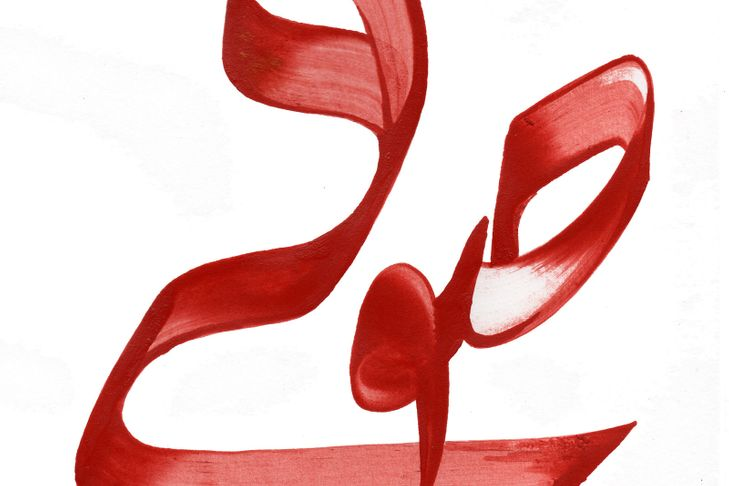
\includegraphics[width=\textwidth]{Images/image013.jpg}


« Aux commencements de l'islam, il n'y a ni ascètes ni soufis.
L'ascétisme et la mystique musulmane vont se développer dans les
sociétés de convertis à partir du IX\textsuperscript{e}~siècle. C'est un
phénomène d'hybridation culturelle. Le soufisme est d'abord le fait de
maîtres isolés au IX\textsuperscript{e}~siècle, vivant du côté de
l'actuel Iran. À partir du XII\textsuperscript{e}~siècle se développent
les premières confréries, dont certaines sont encore vivantes
aujourd'hui. Dans l'islam, la mystique est aussi développée que dans le
christianisme, mais elle a été davantage combattue. D'abord par les
juristes, qui voyaient d'un mauvais œil ces croyants qui s'émancipaient
des règles sociales, puis par le wahhabisme, qui les a massacrés dans la
deuxième­ moitié du XVIII\textsuperscript{e}~siècle ».\sn{Jacqueline Chabbi}


« Dans cette calligraphie, j'ai recherché la stabilité mais aussi un
geste plus tendre. Certains y verront peut-être un personnage
agenouillé, en prière\ldots{} Pourquoi pas ? J'offre une image sur
laquelle je ne peux pas toujours mettre des mots. C'est à ceux qui
regardent d'interpréter mes images. Quand je peins, je prends toujours
en considération le blanc laissé par la trace. En calligraphie, un
principe dit :\emph{~``Le noir de votre calligraphie, c'est vous. Le
blanc de votre calligraphie, c'est vous aussi.''}~J'y pense souvent.
Dans les textes anciens, le soufi -- que l'on peut traduire par
``mystique'' -- doit travailler sur soi-même pour retrouver la lumière
intérieure. Il devient alors pur et peut arriver à rencontrer la
divinité. »\sn{Hassan Massoudy}


\section{Introduction}
\paragraph{ Qu'est-ce que le soufisme~?} Pour les soufis, il s'agit de la dimension
spirituelle et originelle de l'islam. Le mot originel est important~: il
signifie que le soufisme est connaturel à l'islam, qu'il est l'islam. Il
ne s'agit pas d'un développement ultérieur qui aurait eu lieu sous
l'influence du monachisme chrétien ou du šī`isme, mais de l'islam vécu
par Muḥammad et ses compagnons. Donc, pour les soufis, Muḥammad est un
soufi. Les salafs, les anciens, les compagnons de Muḥammad sont soufis.
On comprend que si al-Ġazālī \label{theol:AlGazali27} considère le soufisme comme la voie par
excellence pour aller à Dieu, il n'en demeure pas moins que sous sa
plume la référence aux salafs y est importante.
\mn{Le soufisme et Si'isme

\begin{itemize}
\item
  historiquement, plutôt dans l'islam sunnisme
\item
  dans le si'isme, c'est presque intégré tellement il est naturellement
  spirituel.

  \item
    Dans le cadre duodecimain strict, on ne prie pas les imams
  \item
    Mais en fait, il y a des «~sectes~» qui vont le prier, à commencer
    par le fait qu'on va considérer que c'est le «~l'imam caché~»

  \end{itemize}}
Pour autant, cette affirmation d'éminents soufis n'est pas partagée par
l'ensemble des penseurs de l'islam, et au cours de l'histoire, le
soufisme a pu faire l'objet de critiques, de contestations, de
réfutations plus ou moins virulentes. Certaines des pratiques soufies
ont pu être considérées comme hétérodoxes, innovatrices, non conformes à
l'islam des origines. Ce sont ces accusations récurrentes qui permettent
d'expliquer pourquoi on s'en prend aujourd'hui encore à des mosquées
soufies. 
\paragraph{Le wahhabisme est la matrice idéologique anti-soufie
contemporaine}. Comme nous l'avons vu, il est né en Arabie à partir du
18\textsuperscript{ème} siècle en contestant les confréries soufies
jugées non confirmes à l'islam. Aujourd'hui, l'État islamique de l'Irak
et du Levant, au lendemain de la conquête de Mossoul a distribué aux
habitants une charte comprenant 16 commandements~: à l'article 10, il
est écrit que toutes les manifestations publiques contraires à l'islam
sont interdites (article 10). En 2014, quatre sanctuaires sunnites et
soufis et six mosquées chiites ont été détruites dans la province de
Ninive, sous contrôle des insurgés. La destruction la plus spectaculaire
fut celle du tombeau du prophète Jonas -- Yunus en arabe -- qui a été
réduite à un amas de cailloux.

En Égypte, dans le Sinaï, en décembre 2016, un shaykh soufi et un de ses
disciples sont assassinés par le groupe de l'Etat islamique. Le 24
novembre 2017 l'attentat à la mosquée al-Rawdah de Bir al-Abed fait 305
morts -- à cette mosquée était attachée une \emph{zāwiya} -- édifice
religieux fréquenté par des soufis et des conscrits de l'armée. Cette
mosquée soufie appartient à l'ordre soufi des ǧarirites du nom d'Aïd Abū
Ǧarīr qui a fondé trois loges dans le Sinaï au 20\textsuperscript{ème}
siècle dont celle de Bir al-Abed\sn{Sur la sociologie religieuse
  du Sinaï, voir l'article d'Ismaïl Alexandrani~:
   \url{http://orientxxi.info/magazine/-genealogie-du-djihadisme-au-sinai,0687}}.

\vide{i--duxe9finir-le-soufisme}{%
\section{{Définir le soufisme
}}\label{i--duxe9finir-le-soufisme}}

En guise d'apéritif, écoutez la voix d'Henri Corbin (m. 1978),
philosophe et éminent orientaliste français, spécialiste surtout de
l'islam iranien et de la gnose chiite. \emph{Extrait d'un entretien avec
Bernard Maxime Latour en 1971}.

Définition complexe donc, «~tâche scabreuse~»\ldots{} essayons cependant
de le définir à partir de la manière dont les musulmans eux-mêmes
présentent le soufisme, le \emph{tasawwuf} en arabe.

Pour cela, je vous propose de lire un extrait du livre Traité de
Kalābāḏī, \emph{Kitāb al-ta`arruf li-maḏhab ahl al-tasawwuf} qui a été
traduit par Roger Deladrière\sn{~\textsc{Kalābāḏī}, \emph{Kitāb
  al-taʿarruf li-madhhab ahl al-taṣawwuf} {[}traduction française~:
  Traité de soufisme, Les Maîtres et les étapes, traduit de l'arabe et
  présenté par Roger Deladrière, Paris, Actes-Sud, Sinbad, 1981.}.
Kalābāḏī \label{theol:Kalabadi} est un auteur persan, mort aux environs de 990. Cet ouvrage
cherche à réconcilier le soufisme et l'orthodoxie. C'est un classique,
apprécié de tous. En son introduction, il consacre plusieurs pages à
cerner le sens de soufisme par l'étymologie. C'est un peu dense et
technique, mais tout à fait accessible. En ces derniers cours, ce long
extrait vous permet de prendre contact avec un texte fondamental en
islam et avoir la satisfaction d'y être à peu près à l'aise.
\begin{quote}
    

«~Certains ont soutenu que les soufis furent appelés de ce nom à cause
de la pureté (\emph{safā}') de l'intime de leur être et de l'absence de
souillure de leurs actes. Selon Bichr Ibn al-Hârith, «~le soufi est
celui dont le cœur est pur à l'intention de Dieu~». D'après un autre,
«~le soufi est celui dont le comportement est pur à l'égard de Dieu et
dont le charisme (\emph{karâma}) qui lui vient de Dieu -- que soient
proclamées Sa Puissance et Sa Majesté~! -- est pur~».
\end{quote}
Selon une autre explication, les soufis ont été appelés ainsi parce
qu'ils sont, devant Dieu, au premier rang (\emph{saff}), du fait que de
leurs aspirations (\emph{himam}) s'élèvent jusqu'à Lui, que leur cœur se
tourne avec empressement vers Lui, et que l'intime de leur être se tient
en arrêt devant Lui.

D'après certains, ils auraient été désignés du nom de soufis parce que
leurs caractéristiques sont proches de celles des «~hommes du banc~»
(\emph{ahl al-suffa}) qui vivaient à l'époque de l'Envoyé de Dieu -- que
Dieu prie sur lui et le salue !

Selon d'autres, ils furent nommés soufis parce qu'ils portaient un
vêtement de laine (\emph{sûf}).

Ceux qui rattachent leur nom au «~banc~» (\emph{suffa}) et à la
«~laine~» (\emph{sûf}) expriment ainsi l'apparence extérieure de leur
état spirituel. \paragraph{ Ce sont en effet des hommes qui ont délaissé ce bas
monde}, ont quitté leur demeure, ont fui leurs amis, parcourant les pays,
le ventre creux, dénudés, ne prenant des choses d'ici-bas que
l'indispensable pour avoir une tenue décente et calmer leur faim. Parce
qu'ils ont quitté leur demeure on les appelle aussi «~étrangers~»
(\emph{ghurabâ'}), et à cause de leurs nombreux voyages on les désigne
sous le nom de «~pèlerins~» (\emph{sayyâhûn}). Du fait de leurs
pérégrinations dans les régions désertiques et parce qu'ils prennent
refuge en cas de nécessité dans les cavernes, les autochtones les ont
surnommés «~les hommes des cavernes~» (\emph{chikaftiyya}) car le mot
«~\emph{chikaft}~» dans leur langue désigne une grotte ou caverne.

Les Syriens leur ont donné le nom de «~faméliques~» (\emph{jaw'iyya})
parce qu'ils prennent seulement comme nourriture ce qui maintient les
forces dont ils ont besoin, conformément à la parole du Prophète~:
\begin{quote}
"Des aliments qui maintiennent ses forces devraient suffire au fils
d'Adam".~     
\end{quote}
Sarî Saqatî les a décrits en ces termes~: 
\begin{quote}
    «~Ils mangent
comme des malades, ils dorment comme des gens qui font naufrage, et ils
parlent comme des hommes stupides.~»
\end{quote}

Du fait de leur renoncement à la propriété on les a appelés «~pauvres~».
On avait demandé à l'un d'eux ce qu'était le soufi, et il répondit~:
\begin{quote}
   «~Celui qui ne possède pas et n'est pas objet de possession.~» 
\end{quote}
voulant
dire par là qu'il n'était pas l'esclave des désirs. À la même question,
un autre déclara~: 
\begin{quote}
    «~Le soufi est celui qui ne possède rien et qui, si
jamais il vient à posséder quelque chose, le donne.~»
\end{quote}


À cause de leur vêtement et de leur aspect on leur a donné le nom de
soufis, car ils ne portent pas ce qui est doux au toucher et agréable à
regarder, ce qui serait flatter les passions de l'âme, mais uniquement
une tenue décente, se contentant d'un tissu au poil rugueux et d'une
laine grossière.

Tout cela était la condition des «~hommes du banc~», qui vivaient à
l'époque de l'Envoyé de Dieu. Ils étaient en effet «~étrangers~» et
«~pauvres~», des exilés qui avaient quitté leur demeure et leurs biens.
Abû Hurayra et Fadâla Ibn'Ubayd en firent la description suivante~:

\begin{quote}
   «~Ils tombaient de faim à tel point que les Arabes bédouins les
prenaient pour des fous.~» 
\end{quote}
 Ils étaient vêtus de laine, et, au dire de
certains, cela les faisaient transpirer tellement qu'ils exhalaient
l'odeur des moutons qui ont reçu la pluie. Ceci au point que 'Uyayna Ibn
Hisn dit au Prophète~: 
\begin{quote}
   «~L'odeur de ces gens m'incommode, ne
t'incommode-t-elle point toi aussi~?~» 
\end{quote}


La laine est d'ailleurs aussi le vêtement des prophètes (\emph{anbiyā'})
et la mise des saints. C'est ainsi que, selon la parole du Prophète
rapportée par Abû Mûsâ Ach'âri,
\begin{quote}
    «~ soixante-dix prophètes, pieds nus et
vêtus de manteaux de laine, sont passés par le rocher de Rawlâ, et ils
se rendaient au \emph{Temple Antique} (de la Mecque)~».
\end{quote} 

D'après Hasan
Basrî, «~Jésus -- que la paix soit sur lui -- se vêtait de crin, se
nourrissait des fruits des arbres, et passait la nuit là où il
s'arrêtait.~» Selon une autre tradition d'Abû Mûsâ, le Prophète se
vêtait de laine, prenait des ânes comme monture, et se rendait à
l'invitation des pauvres gens. Hasan Basrî disait encore qu'il avait
connu soixante-dix Compagnons ayant combattu à Badr qui ne se vêtaient
que de laine. Ceux qui se comportaient comme les «~hommes du banc~»,
selon ce que nous avons indiqué, ayant les mêmes vêtements et la même
tenue qu'eux, portèrent donc le nom de «~\emph{suffiyya}~» et du
«~\emph{sûfiyya}~» (soufis).

\paragraph{Quand on rattache leur nom à l'élite (\emph{safwa}) et au premier rang
(\emph{saff}), on exprime alors ce qui se rapporte à leur être intime et
à leur état intérieur}. Dieu, en effet, purifie le secret de l'âme et
illumine le cœur de celui qui quitte le monde, y renonce et s'en
détourne. Selon une parole du Prophète,

\begin{quote}
«~quand la lumière pénètre dans
le cœur, il se dilate et s'épanouit.~» On lui demanda «~quel en est donc
le signe, ô Envoyé de Dieu~?~»~; il répondit «~s'éloigner du monde
illusoire, se tourner vers le monde éternel, et se préparer à la mort
avant qu'elle ne survienne.~»    Ainsi le Prophète avait fait savoir que
Dieu illumine le cœur de celui qui s'éloigne de ce bas monde. Et quand
il questionna Hâritha sur la réalité profonde (\emph{haqîqa}) de sa foi
(\emph{imân}), celui-ci déclara~: «~J'ai détaché mon âme de ce monde,
assoiffé pendant le jour, en veillant la nuit, et ce fut comme si je
voyais se dresser le Trône de mon Seigneur, et comme si j'apercevais les
habitants du Paradis qui se rendaient visite et ceux de l'Enfer qui se
repoussaient.~» Selon ce récit, après qu'il se fut détaché du monde,
Dieu lui illumina le cœur, de sorte que ce qui lui était primitivement
caché lui était devenu visible. Le Prophète s'écria alors~: «~Quiconque
veut voir un serviteur dont Dieu a illuminé le cœur n'a qu'à regarder
Hâritha~!~» À cause de ces caractéristiques, de tels hommes ont été
appelés «~illuminés~» (\emph{nûriyya}). Elles étaient également celles
des «~hommes du banc~». Dieu a dit en effet~: «~Il y a là des hommes qui
aiment à se purifier~; et Dieu aime ceux qui se purifient~.~» Il s'agit
de se purifier extérieurement des souillures et de se purifier
intérieurement des pensées qui surgissent dans l'esprit et des idées qui
se meuvent dans la conscience. Dieu a dit~: «~Des hommes que nul négoce
et nul troc ne distraient de l'invocation (\emph{dhikr}) de Dieu.~»
\end{quote}
 

En outre, à cause de la pureté de leur être intime, leur intuition
(\emph{firâsa}) est juste. Selon une tradition du Prophète rapportée par
Abû Umâma Bâhilî~: «~Prenez garde à l'intuition du croyant, car il
regarde avec la lumière de Dieu~!~» Abû Bakr le Véridique avait
déclaré~: «~Mon cœur a reçu l'inspiration que l'enfant porté dans son
sein par Bint Khârija est une fille~»~; et il en fut comme il l'avait
annoncé. De même le Prophète a dit «~La Vérité parle par la bouche de
'Umar.~» Uways Qarâni, salué par Harim Ibn Hayyân, lui rendit ses
salutations en l'appelant par son nom, alors qu'il ne l'avait jamais vu
auparavant~; et il lui dit ensuite~: «~Mon âme a reconnu ton âme.~» «~Si
vous vous entretenez avec les «~hommes de la sincérité (\emph{sidq}),
dit Abû 'Abd'Allâh Antâki, soyez vous-mêmes sincères, car ils sont les
observateurs des cœurs~! Ils pénètrent dans l'intimité de votre âme et
décèlent vos intentions.~»

\paragraph{Quiconque possède de telles qualités~: limpidité de l'être profond,
pureté du cœur, lumière de l'âme, est «~au premier rang~»}, car elles
caractérisent les «~devançants~» (\emph{sâbiqûn}). Selon une tradition
du Prophète~: «~Soixante-dix mille membres de ma Communauté entreront au
Paradis sans Jugement », précisant ensuite «~pour les autres ou pour
eux-mêmes ils n'ont point de recours aux talismans ni aux
cautérisations, mais ils s'en remettent à leur Seigneur avec
confiance.~» À cause de la pureté de leur être intime, de l'ouverture de
leur âme, et de l'illumination de leur cœur, les connaissances qu'ils
tiennent de Dieu sont justes~; ils ne se réfèrent pas aux causes
secondes (\emph{asbâb}), confiants qu'ils sont en Dieu, s'en remettant à
Lui, et acceptant Son Décret (\emph{qadâ}).

Toutes ces qualités et toutes les significations de ces mots se trouvent
réunies dans les noms et les appellatifs désignant la «~communauté
spirituelle~» (\emph{qawm}). Les expressions en sont exactes, et leur
emploi en est facilement compréhensible. Même s'ils diffèrent en
apparence, leur sens est concordant.

\begin{Def}[soufi]
Si on le tire de \emph{safâ'}
(pureté) et \emph{safwa}(élite), le terme qui désigne ces hommes est
alors celui de \emph{safawiyya}. Si on le rapporte à \emph{saff} (rang)
ou \emph{suffa} (banc), ils sont des \emph{saffiyya} ou des
\emph{suffiyya}.
\end{Def}
 Il est possible, dans le premier cas, que la lettre
\emph{wâw} ait été placée avant la lettre \emph{fâ'}, ce qui donne bien
le mot \emph{sûfiyya}(soufis)~; et, dans le deuxième cas, ajouter le
\emph{wâw} à \emph{saffiyya} ou \emph{suffiyya} serait dû à l'usage
linguistique. Si, enfin, on a tiré le mot \emph{sûfiyya} du \emph{sûf}
(laine), il est parfaitement correct, et cette désignation est
linguistiquement juste.

 \paragraph{Ces termes expriment le renoncement et le détachement
de l'âme à l'égard de ce bas monde, le fait de quitter sa demeure et de
voyager sans cesse, de ne pas flatter les passions de l'âme, de purifier
sa conduite, de rendre limpide l'intime de son être, d'ouvrir son cœur,
et de se comporter en «~devançant~». } Ajoutons à cela ce que dit Bundâr
Ibn Husayn~: «~Le soufi est celui que Dieu a choisi pour lui-même et
qu'Il a traité avec affection (\emph{sâfâ}), le libérant de son âme
(égoïste) et lui épargnant dès lors tout effort et toute contrainte en
vue d'un motif personnel. Et le mot \emph{sûfiya~}= il a été traité avec
affection est (un verbe passif) du même type morphologique que
\emph{'ûfiya}~: il a été protégé, à savoir que c'est Dieu qui l'a
protégé, et \emph{kûfiya~}: il a été rétribué, par Dieu, ainsi que
\emph{jûziya~}: il a été récompensé, par Dieu. L'action de Dieu sur lui
est donc manifeste dans son nom même de \emph{sûfî}, et Dieu est seul à
s'occuper de lui.~»

Interrogé sur la définition du soufi, Abû 'Alî Rûdhabâri répondit~:
«~C'est celui qui a revêtu de laine (\emph{sûf}) sa pureté
(\emph{sâfâ}'), qui a fait goûter à ses désirs personnels la saveur de
la privation, et qui, ayant laissé ce bas monde derrière lui, a suivi la
voie de l'Élu (Mohammad).~»

La même question ayant été posée à Sahl Ibn'Abd Allâh Tustarî~: «C'est,
dit-il, celui qui est pur de tout ce qui trouble, qui est rempli de
méditation, qui s'est retiré des hommes pour se consacrer à Dieu, et
pour qui l'or et l'argile se valent.~»

On demanda à Abû-l-Hasan Nûrî ce qu'était le soufisme
(\emph{tasawwuf})~: «~C'est, répondit-il, délaisser tout ce qui flatte
l'âme.~»

Interrogé sur le même sujet, Junayd définit le soufisme~: «~ C'est
purifier son cœur de l'approbation des hommes, abandonner ses tendance
innées, maîtriser les dispositions de la nature humaine, écarter les
incitations égoïstes, fixer en soi les qualités spirituelles, s'attacher
à la connaissance des réalités immatérielles, utiliser ce qui est mieux
pour la vie éternelle, pratiquer le (devoir de) bon conseil envers la
Communauté tout entière, tenir envers Dieu l'engagement de rester fidèle
à la vérité, et suivre l'Envoyé dans (l'accomplissement de la foi).~»

Selon Yûsuf Ibn Husayn~: 
\begin{quote}
    «~Chaque Communauté a une élite, dépôt précieux
de Dieu qu'Il a caché à Ses créatures, et s'il y en a une dans cette
Communauté-ci, ce sont les soufis.~»
\end{quote}

Quelqu'un demanda à Sahl Ibn `Abd Allâh Tustarî~: «~Qui fréquenterai-je
parmi les différents groupes musulmans~?~» «~Tu n'as qu'à fréquenter les
soufis, répondit-il, car rien n'a à leurs yeux une importance exagérée
et ne saurait être totalement désapprouvé. Pour eux, tout acte peut être
interprété, et ils te trouveront des excuses en n'importe quelle
circonstance.~» La même question ayant été posée par Yûsuf Ibn Husayn à
Dhû-l-Nûn~:
\begin{quote}
«~Fréquente, dit-il, celui qui ne possède rien et qui ne désapprouvera
aucune situation dans laquelle tu pourras te trouver, qui ne changera
pas même si toi tu changes beaucoup, car plus tu changeras, plus tu
auras besoin de lui~!~»
\end{quote}
On rapporte également de Dhû-l-Nûn ceci~:
\begin{quote}
    
«~Au bord de la mer, en Syrie,
je vis, dit-il, une femme, et je lui demandai~: «~D'où viens-tu -- que
Dieu te fasse miséricorde~! -- ~?~» Elle me répondit~: «~D'auprès de
gens qui répugnent à reposer leur corps sur une couche, et qui prient
leur Seigneur avec crainte et désir.~» -- Et où vas-tu~? Insistai-je. --
Vers des hommes «~que nul négoce et nul troc ne distraient de
l'invocation de Dieu. -- Décris-les-moi~! Lui demandai-je. Elle se mit
alors à déclamer ces vers~:

\emph{Des hommes dont les préoccupations s'attachent à Dieu, et dont les
aspirations ne s'élèvent vers personne d'autre.}

\emph{Leur quête est celle de leur Maître et de leur Seigneur, et quelle
noble quête que celle de l'Unique, l'Impénétrable~!}

\emph{Ils ne se disputent rien de ce monde, ni rien de ce qui est
excellent, ni nourritures, ni plaisirs, ni progénitures, ni vêtements
somptueux et élégants, ni la joie reposante de rester au pays.}

\emph{Ils ne luttent qu'à la poursuite du lieu éternel dont chaque pas
les rapproche.}

\emph{Ils courent par les étangs et les vallées, et on les rencontre en
nombre sur les hauteurs.}
\end{quote}
\vide{ii--muxe9thode-spirituelle-du-soufisme}{%
\section{Méthode spirituelle du
soufisme}\label{ii--muxe9thode-spirituelle-du-soufisme}}

C'est un itinéraire spirituel qui vise à remonter vers l'être unique, à
quitter la dualité de l'homme, sa duplicité, en vue d'une unification.
Il s'agit d'abandonner la superficialité des choses pour entrer dans la
profondeur de l'intériorité et ne pas être réduit au monde des
apparences.

Dans son \emph{Essai sur le soufisme}, Martin Lings compare le monde à
une pépinière~: tout ce qui s'y trouve a été planté en vue d'être
transplanté ailleurs. La partie centrale de la pépinière est réservée à
des arbres nobles. Ils sont tous en pot et poussent, pas beaucoup, mais
un peu. Mais quand on regarde bien, un des arbres se distingue des
autres. Il est luxurieux, vigoureux, beau. Que s'est-il passé~? La cause
en est invisible. Pour autant, on la devine~: cet arbre a pris racine
dans la terre du jardin à travers le fond de son récipient. Que dit
cette image~? Les arbres sont des âmes et le soufisme est une méthode,
une voie pour prendre racine, pour passer à travers la porte étroite qui
est dans l'âme elle-même et qui débouche sur l'océan de la Divinité. Le
soufi sait qu'il est comme les autres hommes, il sait aussi qu'il est
prisonnier du monde des formes (les pots), mais il sait aussi qu'il est
appelé à la liberté qui l'emporte sur sa captivité.

Le soufisme doit donc permettre de s'enraciner dans l'océan de la
divinité, d'entrer dans la source de la divinité, dans
l'\emph{\underline{origine}} donc. Cette origine est divine,
transcendantale, c'est celle de l'Absolu, de l'Éternel.

\paragraph{Le soufisme est d'abord une méthode~; il est donc un anti-dogmatisme,}
mais il n'est pas sans dogmes. Il ne nie pas le credo musulman, au
contraire~; les soufis ont une profession de foi qu'ils énoncent. Mais
il s'agit de ne pas limiter Dieu à cette profession. Dans cette optique,
le mystique andalou Ibn `Arabī appelle à ne pas se limiter à un credo
particulier. Voici un extrait des \emph{Chatons de la sagesse.} Vous
reconnaîtrez peut-être la voix de Georges Claisse. Dans la suite du
cours, je reviendrai sur cette très grande figure du soufisme.

Voie spirituelle vers Dieu, le soufisme est donc la définition d'une
méthode afin d'atteindre la proximité de Dieu, mais plus encore chez
certains, une union, une unification.

\vide{limitation-du-prophuxe8te}{%
\subsection{L'imitation du
Prophète}\label{limitation-du-prophuxe8te}}

\begin{Def}[Sainteté, suġrā et kubrā]
Le soufisme comme voie initiatique conduisant à la «~proximité divine~»
(\emph{walāya})~distingue selon la sainteté «~mineure~» (\emph{suġrā}),
ouverte à tous les fidèles, et la sainteté «~majeure~» (\emph{kubrā}),
réservée à une élite. 
\end{Def}
Pour parvenir à cette sainteté, la plupart des
soufis invitent à l'imitation du Prophète dans la mesure où il est celui
qui a réalisé cette parfaite proximité. 
\begin{Def}[\emph{nubuwwa}]
prophétie
\end{Def}

Ils posent donc l'existence
d'une relation entre la \emph{walāya} et la \emph{nubuwwa}, la
prophétie, mais si al-Tirmidhī (m. 318/930) accorde à la \emph{walāya}
son autonomie par rapport à la nubuwwa, d'autres au contraire, affirme
qu'il n'est pas possible de s'approcher de Dieu sans la \emph{nubuwwa}. \sn{la question est donc la possibilité de l'usage de la Raison pour accéder à Dieu}

L'hagiographie du Prophète Muḥammad s'est aussi accompagnée d'une
spiritualisation de sa figure~: il est «~l'Homme universel~»
(\emph{al-insān al-kāmil}) qui demeure dans ceux qui l'imitent. Or, la
participation à la «~sainteté prophétique~» permet d'actualiser la
Révélation, autrement dit dans donner les clefs pour chaque époque. Il
s'ensuit un «~Muhammado-centrisme~» car c'est Muḥammad en tant que sceau
des Prophètes qu'il convient d'imiter, de suivre, et donc à qui il faut
obéir. On voit ici que le rapport à la Loi est loin d'être supprimé,
spiritualisé. Au contraire.

 
\subsection{Le souvenir
(\emph{ḏikr})} \label{le-souvenir-dikr}

Le souvenir (\emph{ḏikr}) est au fondement du soufisme.
\begin{Def}[{ḏikr}]
Souvenir,
rappel, invocation, il s'agit de revenir à Dieu, de sortir de l'amnésie
qui guette l'homme, de retrouver le moment où fut scellé le pacte
originel (\emph{mīṯāq}).
\end{Def}
  Cette invocation convient à tout lieu, elle est
la marque d'une adoration continuelle. Le \emph{ḏikr} permet de
retrouver et de vivre de la présence divine.

Le Coran invite à cette évocation, à ce souvenir~: «~Souvenez-vous de
moi et je me souviendrai de vous~» (S. 2, 152). De même, le \emph{ḥadīṯ}
invite à la pratique du \emph{ḏikr}.

Ainsi, par exemple~:

\begin{itemize}
\item
  «~`Les cœurs rouillent comme le fer' dit le Prophète à ses compagnons.
  `Et qu'est-ce qui les fait briller~?' demande l'un d'eux.
  `L'invocation de Dieu et la lecture du Coran'~».
\item
  «~Celui qui invoque son Seigneur et celui qui ne l'invoque pas sont
  comparables l'un à un vivant, l'autre à un mort~».
\end{itemize}

Concrètement, le \emph{ḏikr} consiste à invoquer les noms divins ou à
répéter la première partie de la formule de la \emph{šahāda}~: \emph{lā
ilāha illā Llāh}. Puis, il s'agit de répéter le mot Allāh seul, puis, la
dernière lettre de Allāh, le h\ldots{} dans un seul souffle.

Je vous propose d'écouter {une séance de
\emph{ḏikr}
\url{https://www.youtube.com/watch?v=Xq6bIVtCq14}}\emph{.} 
. Ici, les soufis chantent
ensemble la formule \emph{lā ilāha illā Llāh} sur laquelle se surajoute
une psalmodie. Le rythme s'accélère et indique une forme d'ivresse
spirituelle. Généralement, ces invocations s'accompagnent du balancement
de la tête de gauche à droite et du mouvement des bras.

\url{https://www.youtube.com/watch?v=9BaQunfXPpE}{Ici}, vous avez une
vidéo d'une séance de \emph{ḏikr} dans une confrérie.

\vide{luxe9coute-de-luxe9cho-du-verbe-divin-samux101}{%
\subsection{L'écoute de l'écho du verbe divin
(samā`)}\label{luxe9coute-de-luxe9cho-du-verbe-divin-samux101}}

\begin{Def}[{samā`}]
Le \emph{samā`}, tout comme le \emph{ḏikr} a pour objectif de
réactualiser le Pacte originel. Il s'agit d'écouter la musique comme un
écho de ce pacte scellé. 
\end{Def}
Par la musique, l'écoutant libère son âme pour
trouver Dieu. Il y a une quête d'extase~: c'est le \emph{tawāǧud}. La
fin recherchée n'est pas la musique, mais l'écoute, la musique n'étant
qu'un support pour entendre la parole divine. L'écoute est donc
éminemment spirituelle~mais l'usage de la musique peut être dévoyé et
tombé dans le divertissement. Le soufisme n'est pas en soi favorable à
l'écoute de la musique mais il ne refuse pas usage à des fins
spirituelles. Al-Ġazālī  \label{theol:AlGazali28} considère que le samā` n'est pas en soi licite
ou illicite, et que tout dépend de l'intention (\emph{niyya}) de
l'écoutant. Pour rendre compte de cette ambivalence, le soufi al-Šiblī
(m. 946), connu pour ses excentricités paradoxales, dit du \emph{samā`}
qu'il est 
\begin{quote}
    «~en apparence une source de trouble, mais qu'il recèle un
grand enseignement spirituel (
\TArabe{
السماع ظاهره فتنة، و باطنه عبرة
})
~».
\end{quote}

L'histoire du \emph{samā`} montre qu'il a été associé à la danse, et
qu'il a été aussi assimilé au \emph{ḏikr}.

Ultime remarque~: le \emph{samā`} est une voie, une méthode soufie, mais
il n'est pas reconnu par tous les soufis et bien des maîtres ont aussi
privilégié le silence absolu tels Ibn `Arabi ou les premiers maîtres
šāḏilis.

\vide{la-repentance-tawba}{%
\subsection{{La repentance
(\emph{tawba})}}\label{la-repentance-tawba}}

Le repentir consiste à regretter son péché. Les soufis insistent sur
l'importance des larmes.

Elles sont aussi pleines de signification~: la larme est la goutte qui
s'efface en s'évaporant, après avoir témoigné. Sa disparition est
littéralement une extinction (\emph{fanā'}). Elle est symbole
d'intercession et de transformation\sn{On retrouve chez les
  Aztèques ce symbolisme~: les larmes des enfants que l'on apporte au
  sacrifice étaient dites annonciatrices de la pluie à venir. De même
  les lamentations sont mises en relation avec la miséricorde divine et
  la descente de la manne céleste.}.

Dans le soufisme, les pleurs symbolisent la quête du soufi de vouloir
s'abreuver à la source divine elle-même, de faire descendre la grâce, de
réaliser ainsi la présence divine. Les larmes ne sont pas négatives,
mais elles sont signe d'une espérance, de la promesse d'une joie à
venir. Elles ne sont pas la manifestation d'une séparation d'avec Dieu,
mais surtout un appel à retrouver Dieu, à s'unir à lui.

\vide{la-retraite-spirituelle-ux1e2balwux101}{%
\subsection{{La retraite spirituelle
(\emph{ḫalwā})}}\label{la-retraite-spirituelle-ux1e2balwux101}}

La retraite spirituelle constituait à l'époque antique un «~exercice
spirituel~». Le texte apocryphe intitulé \emph{La théologie d'Aristote}
écrit très vraisemblablement en syriaque au VI\textsuperscript{ème}
siècle et qui est un commentaire (\emph{tafsīr}) de certains passages
des \emph{Ennéades} de Plotin\sn{Pierre Thiellet, «~Notes sur la
  Théologie d'Aristote~» dans Prophyre, \emph{La vie de Plotin}, II,
  Paris, Vrin, 2000, p. 625-638.}, donne pour définition de l'extase le
fait d'être seul avec son âme (\emph{khalawtu bi-nafsi})\sn{Plotin,
  \emph{Ennéades}, IV, 8, 1.}. Il exerça très probablement une influence
dans la théorisation de cette solitude spirituelle. La pratique de la
retraite dans le soufisme renvoie à celle du monachisme chrétien avec
les Pères du désert, où l'éloignement de la ville et de la société était
considéré comme un chemin vers Dieu et un des fondements de l'ascétisme
(\emph{zuhd}). Depuis la \emph{Risāla} d'Abū al-Qāsim al-Qušayrī
(986-1072), toutes les présentations du soufisme intègrent un chapitre
sur les retraites spirituelles, qu'elles soient permanentes ou
périodiques. On appelait ces retraites des «~quarantaines~»
(\emph{arba`īniyya}). Elles étaient comprises comme une \emph{imitatio
prophetae}, à la suite de la retraite de quarante jours de Moïse sur le
mont Sinaï ou de celle de David pour réparer sa faute ou encore bien sûr
de Muḥammad qui allait une fois par an se recueillir (\emph{tahannuṯ})
sur le Mont Ḥirā'\sn{Paul B. Fenton, «~La pratique de la retraite
  spirituelle~», dans Giuseppe Cecere, Mireille Loubet, Samuela Pagani,
  \emph{Les mystiques juives, chrétiennes et musulmanes dans l'Égypte
  médiévale (VII\textsuperscript{e}-XVI\textsuperscript{e} siècles).}
  Interculturalités et contextes historiques, Le Caire, IFAO, 2013, p.
  211-252.}. Vous vous souvenez, c'est pendant un temps de retraite
qu'il reçut la révélation du Coran.

Au livre seizième de l'\emph{Iḥyā'} sur la retraite et la vie retirée
(\emph{`uzla}), al-Ġazālī \label{theol:AlGazali29} indique l'existence d'un débat au sein de la
deuxième génération des musulmans~: certains recommandaient en effet
l'amitié, l'assistance entre les croyants, la fraternité, tandis que
d'autres soulignaient l'importance de l'isolement et de la retraite
spirituelle. «~Fuis les gens comme si tu fuyais le lion~»\sn{\textsc{Al-Ġazālī },
  \emph{Iḥyā' `ulūm al-dīn, op. cit.,} K. 16 (\emph{Kitāb ādāb
  al-`uzla}), B.1, p. 665 {[}V.4, p. 248{]}.} conseille Dawūd al-Ta'i.
On raconte aussi cette histoire à propos de Sahl Ibn al-Ṭustarī (m.
896), grand maître soufi~\sn{\emph{Ibid}., p.666 {[}V.4, p. 251-252{]}}.:
\begin{quote}
    
«~Alors qu'un homme s'avança et lui dit qu'il
voulait lui tenir compagnie, Sahl lui répondit~: `Et si l'un de nous
deux vient à mourir, qui sera le compagnon de l'autre~?' L'homme lui
dit~: `Dieu'. Sahl reprit la parole~: `Qu'il lui tienne donc dès à
présent compagnie'~»
\end{quote}

Mais cette approche spirituelle de la retraite et de la solitude dans la
prière et l'isolement a aussi ses détracteurs. En opposition, on
rapporte les paroles du Prophète Muḥammad~où l'on retrouve le bestiaire
du désert~:

\begin{quote}
«~Satan est un chacal pour l'homme. Comme le chacal il saisit du
troupeau la bête égarée qui s'en est éloignée. Prenez garde aux vallées
et restez attachés aux communautés, aux groupes et aux mosquées~».
\end{quote}

Plus rédhibitoire, ce propos du Prophète de l'islam~\sn{\emph{Ibid}, B.1, ḏ.1, p. 667 {[}V.4, p.
  253-254{]}.}: 
\begin{quote}
   «~celui qui se
sépare du groupe (\emph{ğamā`a}), ne serait-ce que d'un empan, ôte de
son cou l'attache de l'islam » ou encore «~celui qui se sépare du groupe
et meurt mourra en homme de l'époque de l'ignorance
(\emph{ğāhiliyya})~». 
\end{quote}

\paragraph{Quels sont les bienfaits attendus de l'isolement~?}
La retraite permet de se consacrer à l'adoration, à la méditation en se
mettant en confidences intimes (\emph{munāğāt}) avec Dieu, en
privilégiant donc l'intimité avec Dieu plutôt qu'avec une créature.

La retraite permet aussi de se débarrasser des péchés auxquels on
s'expose en fréquentant les gens~: la calomnie, la médisance, la
bigoterie, la duplicité, l'avidité, l'attachement au bas-monde.
Al-Ġazālī \label{theol:AlGazali30} indique que l'habitude des gens consiste à se rincer la bouche
avec l'honneur des gens. La fréquentation conduit à s'accorder avec eux
et à s'exposer à la colère de Dieu. Garder le silence revient à
s'associer à leur médisance car l'auditeur est un médisant. Les récuser,
c'est s'exposer à se faire détester et susciter médisance et calomnie
contre soi, donc la médisance en est redoublée\ldots{}\sn{\textsc{Al-Ġazālī },
  \emph{Iḥyā' `ulūm al-dīn}, \emph{op. cit.,} K. 16, B.2, p. 673 {[}V.4,
  p. 272{]}~}.

La fréquentation des gens nous fait poser des questions vides et
hypocrites. Ainsi quand on voit quelqu'un, on lui demande «~comment ça
va~?~», mais on n'accorde aucune importance à la réponse. L'intérêt que
l'on porte à l'autre dans cette question est faux. Autrement dit, la
fréquentation des gens nous pousse à la duplicité. Al-Ġazālī \label{theol:AlGazali11} voit dans
cette question une innovation blâmable.

Finalement, le critère qui permet de vérifier si la retraite est
\emph{ḥarām} ou \emph{ḥalāl} est celui du bien que l'on retire de
l'autre~de par son beau caractère : «~si tu trouves un convive
(\emph{ğalīs}) qui te rappelle l'image et la conduite de Dieu, alors
attache-toi à lui\ldots{} car c'est là le trésor de l'homme doué de
raison (\emph{ġanīmat al-`āqil})~et le dessein du croyant (\emph{ḍāllat
al-mu'min}) »\sn{\textsc{Al-Ġazālī }, \emph{Iḥyā' `ulūm
  al-dīn}, \emph{op. cit.,} K. 16, B.2, fa.2, p. 677 {[}V.4, p. 285{]}~}.

Troisième bienfait~: celui de l'esprit de querelle et du fanatisme. On
rapporte ce dit de Muḥammad~:
\begin{quote}
    «~Il y aura une époque où pour préserver
sa religion, il faudra fuir de village en village, du sommet d'une
montagne à un autre, d'une pierre à une autre, comme un renard qui
s'échappe. Ce jour-là arrivera quand on ne gagnera sa vie qu'en
commettant des péchés et en désobéissant à Dieu. Alors, à cette époque,
le célibat (\emph{`uzūba}) deviendra licite~»\sn{\textsc{Al-Ġazālī },
  \emph{Iḥyā' `ulūm al-dīn}, \emph{op. cit.,} K.16, B.2, fa.3, p. 677
  {[}V.4, p. 286{]}.}.
\end{quote}

Cependant, al-Ġazālī est le théoricien soufi du juste milieu. Et il
souligne combien vivre en dehors de la communauté peut être l'occasion
de s'enorgueillir. Ainsi, en est-il de cette histoire juive~:

\begin{quote}
«~Un sage {[}parmi les israélites{]} avait rédigé trois cent soixante
opuscules sur la sagesse, si bien qu'il en était venu à penser qu'il
avait été gratifié d'un degré élevé auprès de Dieu. Dieu révéla à son
prophète~: `Va lui dire qu'il a rempli la terre d'hypocrisie et que je
n'agrée en rien son hypocrisie'. Le sage abandonna alors
{[}l'écriture{]} et se retira dans un tunnel sous terre. Il se dit en
lui-même~: `À présent, j'ai atteint le contentement de mon Seigneur.
Mais Dieu révéla à son prophète la parole suivante~: `Dis-lui qu'il
n'obtiendra mon contentement qu'après avoir fréquenté les gens et
supporté leur nuisance'. Le sage quitta son refuge et entra dans les
marchés pour fréquenter les gens, s'asseoir avec eux, partager leurs
repas, déambuler dans les marchés. Dieu révéla alors à son prophète~:
`Maintenant, il a obtenu mon contentement~»\sn{\textsc{Al-Ġazālī },
  \emph{Iḥyā' `ulūm al-dīn}, \emph{op. cit.,} K. 16, B.2, p. 687 {[}V.4,
  p. 312{]}.}.
\end{quote}

Si le soufi doit se retirer dans une cellule en solitude, si c'est là
qu'il se souvient de Dieu, l'enjeu est de parvenir à un état permanent
de retraite intérieure. La démarche se retrouve chez Muḥammad.

Le šayḫ al-`Alawī, soufi algérien qui appartient à la branche
confrérique Šaḏiliya qui a pris naissance au 14\textsuperscript{ème}
siècle et qui met l'accent sur l'invocation du nom de Dieu, a fondé sa
propre confrérie. Sa méthode bien qu'elle s'inscrive pleinement dans
l'esprit de la Šaḏiliya, est aussi originale~:

\begin{quote}
«~La khalwah est une cellule dans laquelle je place le novice après
qu'il a juré de ne pas la quitter pendant quarante jours si besoin est.
Dans cet oratoire, il ne doit rien faire d'autre que répéter
continuellement le nom divin (Allâh) en prolongeant à chaque invocation
la syllabe âh jusqu'à ce qu'il soit à bout de souffle.\\
Préalablement, il doit avoir récité la \emph{shahâdah} (\emph{lâ ilâha
illa Llâh}, « il n'y a de Dieu que Dieu ») soixante-quinze mille fois.

Durant sa retraite, il jeûne rigoureusement tout le jour, ne rompant son
jeûne qu'entre le coucher du soleil et l'aube\ldots{} quelques foqarā'
(mystiques) obtiennent l'illumination soudaine au bout de quelques
minutes, d'autres seulement après plusieurs semaines. Je connais un
\emph{faqîr} qui a attendu huit mois. Chaque matin, il me disait: « Mon
cœur est encore trop dur », et il poursuivait sa ḫalwā. À la fin, ses
efforts furent récompensés. »\sn{Martin Lings, \emph{Un saint
  musulman}, p. 96.}
\end{quote}

\vide{station-maqam-et-uxe9tat-ux1e25ux101l-spirituel}{%
\subsection{{ Station (\emph{maqam}) et état
(\emph{ḥāl}) spirituel
}}\label{station-maqam-et-uxe9tat-ux1e25ux101l-spirituel}}

Il existe dans le soufisme une théorie des états et des stations
spirituelles qui dessinent le cheminement et la progression du soufi.
\begin{Def}[\emph{maqam} (station)]
représente dans l'itinéraire vers Dieu, un
degré de perfection spirituelle obtenu à la suite de l'effort personnel
du mystique.
\end{Def}

 Le \emph{ḥāl} (état) en revanche consiste en une
disposition que l'on ne doit qu'à Dieu: «~Les états, disait Al Qushayrī,
sont des dons, les stations sont des mérites~».
\begin{Def}[\emph{ḥāl}]
Le \emph{ḥāl} est fondamentalement un état passager, éphémère. Le but du
soufi est de transformer le \emph{ḥāl} en état permanent (\emph{maqām}).

\end{Def}
Il faut passer du conjoncturel au structurel. Ainsi, la crainte peut
saisir le croyant à la lecture d'un passage du coran, suite à la
rencontre avec un savant ou un soufi\ldots{} mais cette crainte
ressentie doit habiter le croyant au-delà d'une sensation. Le combat
consiste donc à rendre permanent le \emph{ḥāl}.

\vide{iii--grandes-figures-soufies}{%
\section{{Grandes figures soufies
}}\label{iii--grandes-figures-soufies}}

\vide{ux1e25asan-al-baux1e63rux12b-643-728}{%
\subsection{Ḥasan al-Baṣrī
(643-728)}\label{ux1e25asan-al-baux1e63rux12b-643-728}}

Il est, selon les historiens arabes, le premier soufi. Il semble
cependant avoir été plus ascète que mystique~: il recommandait le mépris
du monde, l'examen de conscience. Pour lui, les spirituels se
reconnaissent à leur désir de Dieu. Il faut savoir se taire~: car parler
rajoute quelque chose à l'absolue transcendance de Dieu et finit par
l'offenser.

Ḥasān al-Basrī n'emploie pas le mot \emph{ḥubb} (amour réciproque). Il
dit~: 
\begin{quote}
    comment je peux dire que Dieu a un amour pour moi~?
\end{quote}
 Il préfère
donc le mot \emph{`išq}~: c'est l'éros, le désir. Mais ce mot ne se
trouve pas dans le Coran. Et le théologien hanbalite al-Ansarī le
refuse. Il y voit une intrusion de la raison humaine. Un bel exemple de
pluralisme en islam sur la question de l'amour de Dieu.

À noter que si le salafisme-wahhabiste combat le soufisme, les
salafistes reconnaissent à Ḥasan al-Baṣrī une autorité en tant
que~transmetteur de nombreux \emph{ḥadīṯs}.

\vide{rux101bia-m.-185801}{%
\subsection{{Rābi`a (m. 185/801)
}{3.2 Rābi`a (m. 185/801) }}\label{rux101bia-m.-185801}}

Elle est la première femme mystique de l'islam, la première soufie, un
premier témoin avec Ḥasan al-Basrī. Elle est née 60 ans après la mort du
Prophète Muḥammad. Il y a deux dates pour sa mort, la première la fait
mourir au milieu du huitième siècle à 55 ans, la seconde à la fin du
huitième siècle à 90 ans. Elle a initié la science de l'amour \emph{`ilm
al-maḥabba.}

Rābi`a n'est pas un prénom, cela veut dire la quatrième~: son milieu
familial était très pauvre et comme elle est la quatrième à être née,
son père l'a appelée La Quatrième. On sait peu de choses sur sa vie de
jeune femme. Fut-elle flûtiste~? prostituée~? Certains biographes le
suggèrent donnant au personnage une plus grande renommée.

Dans l'histoire de la pensée, elle est citée par les grands théologiens.
Ainsi, par exemple, Ğāḥiẓ (m. 867) parle d'elle dans le \emph{Livre des
animaux}. Il rapporte le propos de Rābi`a alors qu'on lui offrait un
esclave pour la servir et elle s'y opposait~: «~J'aurais honte de
demander des biens de ce monde à Celui à qui ils appartiennent ; comment
dès lors les solliciterais-je de gens à qui ils n'appartiennent pas ?~».

Ǧāḥiẓ a souligné la qualité rhétorique du propos (il est spécialiste de
rhétorique) ; il y reconnaît en arabe une éloquence exceptionnelle, une
prouesse rhétorique, mais aussi
une preuve ontologique contre l'esclavage.

Un exemple très connu est celui des deux seaux d'eau~ et des charbons~:
Ici, vous allez entendre la voix de Salah Stétié, un écrivain libanais
qui a traduit dans un français remarquable ses plus beaux poèmes.


\subsection{Pour aller plus loin~: les femmes soufies}

Sulaymī consacre un petit opuscule intitulé \emph{Les femmes soufies},
seconde moitié du 10\textsuperscript{ème} siècle, après le traumatisme
de Ḥallāğ \\


Quelques paroles «~insolentes~»~ (l'expression et de Salah Stétié)

\emph{Sur le paradis}

«~Un jour on récitait devant elle ce verset du Coran~: `Ce jour-là, la
seule occupation des hôtes du paradis sera de se réjouir en compagnie de
leurs épouses, ils se tiendront sous des ombrages, accoudés sur des lits
d'apparat'. Elle dit~: `pauvres gens du paradis, les voilà bien occupés
de leurs femmes~!'~»

\emph{Sur le Prophète}~

«~Aimes-tu le prophète~? Certes je l'aime, mais l'amour du créateur m'a
détourné définitivement de l'amour de toute créature~»

\emph{Sur les deux amours}

\begin{quote}
Je t'aime de deux amours

Amour de mon bonheur et amour digne de toi

Quant à cet amour de mon bonheur

c'est que je m'occupe à ne penser qu'à toi seul

à l'exclusion de tout autre

Et quant à cet autre amour dont tu es digne

C'est mon désir

Que tes voiles tombent et que je te voie

Nulle gloire en moi en l'un en l'autre,

non mais louange à toi pour celui-ci comme pour celui-là\sn{Traduction
  Salah Statié, \emph{Rabi'a de feu et de larmes,} Fata Morgana, 2010.}.
\end{quote}

\emph{Sur le pardon}

«~On lui demande~: `J'ai commis de nombreux péchés, Dieu me
pardonnera-t-il si je me repens~?' Elle répond~: il faut que Dieu te
pardonne d'abord et ensuite tu te repentiras~».

\begin{quote}
Ma coupe, mon vin, mon hôte, sont trois,\\
Et moi que remplit l'amour : je suis la Rabi'a\\
Celui qui verse le vin fait circuler sans cesse\\
la coupe de la volupté et du luxe\\
Si de mes yeux je vois, je ne vois que pour Lui,\\
Si regardée je suis, je suis vue avec Lui.\\
O ! Toi qui me blâmes ! Sa beauté oui, je l'aime~!\\
et par Dieu, mes oreilles n'ont que faire de Ton blâme.\\
Que de nuits délirantes j'ai passées, feu, tourment,\\
et mes yeux se sont fait sources par mes larmes !\\
et aucune de mes larmes n'a pu remonter à sa source\\
mon union avec Lui n'a pas duré.\\
blessé, meurtri, mon œil plus jamais ne s'apaise
\end{quote}

\vide{al-hallux101ux11f-m.-309-922}{%
\subsection{al-Hallāğ (m. 309 /
922)}\label{al-hallux101ux11f-m.-309-922}}

C'est un personnage complexe dont l'évolution religieuse a fait couler
beaucoup d'encre. Louis Massignon lui a consacré sa thèse doctorale.
C'est un mystique musulman, crucifié, criant du haut de sa croix~: «~Je
suis Dieu~»\ldots{} expression de sa doctrine de l'unification
(\emph{ḥulūl}).

Son nom lui vient du métier de son père~qui était cardeur de coton. Ses
disciples l'appelaient \emph{al-Hallâj al-asrâr} c'est-à-dire le cardeur
des pensées secrètes. Il voulait dévoiler les «~secrets de l'union
divine~» (\emph{asrār al-tawḥīd})\sn{Pour sa biographie, je
  m'appuie notamment sur l'introduction de Stéphane Ruspoli : \emph{Le
  Message de Hallâj l'Expatrié}, Collection Patrimoine Islam, Paris,
  Cerf, 2006.}.

Quelles relations entretenait-il avec le calife Mu'tadid (892-902) puis
le calife Muqtadir (m. 932) qui le laissa exécuter~? Quels furent ses
contacts avec le christianisme~? Dans quelle mesure trouva-t-il dans la
figure du Christ et de sa Passion un modèle, alors même que l'islam
réfute la mort sur la Croix de Jésus~? Dans quelle mesure ses voyages au
Cachemire lui ont-ils permis de s'imprégner de la sagesse hindoue~?

Il passera une année entière de retraite à La Mecque, imitant ainsi les
retraites solitaires de Muhammad sur le mont Hira. C'est un prédicateur,
un enseignant. Pour lui, l'islam «~n'est pas seulement la soumission
passive~» devant Dieu, ni l'obéissance aux rites prescrits, mais une
doctrine du salut, de la connaissance, de l'amour~». Il était partisan
de la voie du blâme, et assumait ses provocations. Il disait~ainsi :
«~La mécréance et la foi se distinguent seulement par leur nom, mais en
réalité il n'y a pas de différence entre les deux~». En 902, suite à une
expérience spirituelle très forte, il a la révélation du Nom Suprême de
Dieu. Cette révélation fut à la base d'une profonde mutation. Il résume
sa quête en une formule~: «~Anâ al-Haqq~» - littéralement «~je suis le
Vrai~», je suis Dieu.

 
\paragraph{Ibn Atā}\label{ibn-atux101}

Il est dénoncé comme agitateur politique, accusé de comploter contre la
sûreté de l'État et de tenir des propos hérétiques, blasphématoires. Il
est arrêté en 913. Il comparaît devant le vizir Alî ibn `Îsâ qui le
jugea après interrogation «~complètement ignorant du Coran et des
sciences annexes, droit canonique (\emph{fiqh}), Tradition
(\emph{Sunna}), poésie et philosophie arabe~»\sn{Stéphane Ruspoli,
  \emph{op. cit}. p. 34.}. «~On croit rêver~»~! Ibn Atā convoqué au
tribunal déclara Hallāǧ innocent des charges dont on l'accusait et
déclara sa profession de foi totalement valide. Fou de rage, le ministre
le fit battre et Ibn Atā mourut une semaine plus tard.

Hallāǧ arrive au supplice. Il a 65 ans. Il récite encore quelques vers
du Dîwân. Il fait sa prière sous les yeux de ses compagnons en disant~:
«~Ne vous inquiétez pas de cette affaire, car je reviendrai parmi vous
après trente jours~». Il est crucifié. La forme de la crucifixion dans
sa forme musulmane vient des Perses sassanides qui la pratiquaient
couramment. Elle est plus violente, brutale, spectaculaire que la
crucifixion romaine. Sa prière avant de mourir est marquée par la
compassion et la résignation.

Son biographe Stéphane Ruspoli commente~: «~On aura appliqué à la lettre
contre un des plus grands saints musulmans qui lutta pacifiquement pour
la cause de l'islam et la gloire de Dieu, ce verset sombre du Qoran~:
«~Ceux qui combattent Dieu et son Envoyé, et qui sèment la corruption
sur la terre, leur rétribution sera d'être tués, ou crucifiés~; qu'on
leur tranche les mains et les pieds, ou bien qu'on les bannisse du
territoire. Ce sera leur sanction ici-bas, tandis qu'un grand châtiment
les attend dans l'autre monde~» (5, 33)~» (p.35).

Quelques extraits de ses poèmes

\emph{\textbf{Kâna li qablî ahwâ (p. 101)}}

\begin{quote}
\emph{J'ai abandonné aux gens leur usage et leur religion}

\emph{pour me dédier à ton amour, toi ma religion et mon usage.}
\end{quote}

\emph{\textbf{Al-`ayn tubsiru (p. 102)}}

L'œil aperçoit Celui qu'il aime et puis le perd de vue,

Mais le regard du cœur ne cesse jamais de le contempler.

Quand Il n'est pas avec moi, son souvenir m'accompagne,

et le cœur le voit toujours, bien qu'Il se dérobe à mon œil.

\emph{\textbf{Tala'at as-shams (p. 109).}}

\begin{quote}
Le soleil de Celui que j'aime s'est levé de nuit,

Il a brillé sans plus connaître de couchers.

Le soleil du jour se couche certes la nuit,

Mais le soleil des cœurs ne saurait se coucher.

Celui qui aime le Bien-Aimé vole vers Lui,

si grand est son désir d'aller à sa rencontre.
\end{quote}

\emph{\textbf{Li'l `ilm ahl (p. 128)}}

\begin{quote}
Je suis un orphelin, et pourtant j'ai un Père que j'invoque.

Mon cœur tant que je vis s'afflige de son absence.
\end{quote}

Remarquez qu'il s'adresse ici à Dieu avec le nom de Père.

\emph{\textbf{Anâ man ahwâ (p. 129)}}

\begin{quote}
Je suis devenu Celui que j'aime et Celui que j'aime est devenu moi

Nous sommes deux esprits habitant en un même corps.
\end{quote}

\emph{\textbf{Tafakkartu (p. 153)}}

\begin{quote}
j'ai longuement réfléchi aux diverses religions en tâchant de les
assimiler,

puis je les ai ramenées à un seul Fondement ayant maintes ramifications.

Ne demandez pas à un seul homme de s'en tenir à un culte déterminé,

car cela l'écarterait certainement du Fondement divin assuré.

Ce qu'il réclame, c'est un Fondement lui permettant d'élucider

les nobles idéaux et les hautes conceptions afin de les réaliser.
\end{quote}

\emph{Commentaire~}: Ici, l'universalisme religieux de Hallâj semble
accepter tous les cultes, sachant que tout vient de Dieu qu'il est la
sève, l'essence, le Fondement (\emph{al-asl}) qui se transmet aux
ramification de la foi (\emph{shu'ab al-îmân}).

\vide{ibn-arabux12b-m.-1240}{%
\subsection{Ibn `Arabī (m. 1240)}\label{ibn-arabux12b-m.-1240}}

C'est un maître soufi. Incontournable. Pour lui, la pensée de Hallāǧ
accuse une certaine dualité au moment de l'union qui se trouve résolue
dans l'unification. Sur ce point, Ibn `Arabī lui reproche d'avoir laissé
survivre cette dualité dans l'expérience de l'union. Pour lui, l'homme
n'est plus une négation pure qui montre et démontre la puissance de
l'affirmation de l'un, mais par son existence nécessaire, il est l'image
de son créateur, il le représente.

La création est le néant par essence. Elle est illusoire. Elle ne sera
jamais le réel éternel~: «~Tu prétends qu'un autre qu'Allah puisse jouir
de l'Existence~: c'est le nier, et tu es formellement coupable
d'idolâtrie~». (cf. Léo Schaya, \emph{La doctrine soufique}, p 30).

Dieu est au-delà de la dualité de l'être et du non-être. On ne peut pas
justifier l'existence de la dualité entre Lui et un autre que lui. Il
rejette la distinction entre cause et effet. Tout ce qu'il a créé est
une manifestation de lui.

Le maître a influencé des confréries (\emph{turuq}) notamment la
Ḫalwatiyya. Il représente la tradition savante du soufisme. Pourquoi~?

C'est complexe. Mais il existe des facteurs explicatifs. Ainsi, Ibn
`Arabī aurait prédit la victoire des Ottomans et la conquête de la
Syrie. Il s'ensuit que la dynastie lui a accordé un patronage.

Mais plus sérieusement, l'évolution du soufisme au
13\textsuperscript{ème} siècle, le développement des confréries ont créé
un appel d'air doctrinal. Les fondateurs de ces branches confrériques
que sont al-Jîlânî, al-Shâdhilî, al-Rifâ'ī, al-Badawi\ldots{} tracent
une voie, donnent une orientation spirituelle à leur postérité
initiatique. Mais il n'y a pas d'enseignement substantiel~: Ibn `Arabi
vient compléter ce vide\sn{Chodkiewicz, p. 36.}.

Son enseignement procède fondamentalement du Coran~: «~Tout ce dont nous
parlons dans nos séances procède du Coran et de ses
trésors~»\sn{Chodkiewicz, p. 40.}. Ainsi, il invite son disciple
de sa manière~:
\begin{quote}
«~Plonge dans l'océan du coran si ton souffle est assez puissant/ Et
sinon, borne-toi à l'étude des ouvrages qui en commentent le sens
apparent mais n'y plonge pas~! Tu y périrais car l'océan du Coran est
profond et si celui qui y plonge ne se limitait aux lieux les plus
proches du rivage il n'en reviendrait jamais vers les créatures. Les
prophètes et les héritiers-gardiens (\emph{al-waratha al-hafaza})
prennent ces lieux pour but par miséricorde pour l'univers. Quant à ceux
qui restent en arrêt (\emph{al-wāqīfūn}), qui sont parvenus au but mais
sont restés là sans jamais revenir, nul ne tire profit d'eux et ils ne
tirent profit de personne~: ils ont visé le centre de l'océan -- ou
plutôt c'est lui qui les a visés -- et ils ont plongé pour
l'éternité~»\sn{Chodkiewicz, p. 43.}.
    
\end{quote}

\textbf{On ne soulignera jamais assez l'importance de la lettre comme fondement
de l'interprétation.} Sans la lettre, pas d'interprétation, pas de sens
caché. Et l'accès à cette lettre est réservé à ceux qui ont du souffle.
Ils ne cherchent pas l'au-delà de la lettre ailleurs que dans la
lettre~!

À la question de savoir comment trouver Dieu, il prend l'exemple de
Moïse et de la révélation de Dieu dans le Buisson ardent~: Moïse était à
la recherche d'un feu (S. 20, 10). Tout besoin, toute quête de Dieu, se
manifeste, s'épiphanise sous la figure de son besoin. Mais, dit Ibn
`Arabī~: l'homme qui est dans le désert et a été abusé par un mirage,
qui finit par désespérer de tout, alors celui-là trouve vraiment
Dieu\sn{Chodkiewicz, p. 62.}. «~Dieu ne peut être trouvé que dans
l'absence des choses {[}c'est-à-dire des causes secondes{]} sur
lesquelles nous prenons appui~».

Sur les autres religions~: il dit qu'il faut traiter les livres des
autres religions à égalité.

Chaque croyance est à considérer car elle est aussi singulière que
chaque manifestation de Dieu. Dans son acte de foi, le cœur du croyant
répond au désir de Dieu de se manifester en lui.

Le «~Poème `La religion de l'amour'~»\sn{Ibn `Arabî,
  \emph{Turjumân al-ashwâq}, extrait du poème 11 avec commentaire du
  Cheikh al-Akbar -- qu'Allâh l'agrée~! Traduit par M. Gloton dans
  \emph{L'Interprète des désirs}, Albin Michel p. 147 et 155-158.}~:

\begin{quote}
\emph{Mon cœur est devenu capable}

\emph{D'accueillir toute forme.}

\emph{Il est pâturage pour gazelles}

\emph{Et abbaye pour moines~!}

\emph{~}

\emph{Il est un temple pour idoles}

\emph{Et la Ka'ba pour qui en fait le tour,}

\emph{Il est les tables de la Thora}

\emph{Et aussi les feuillets du Coran~!}

\emph{~}

\emph{La religion que je professe}

\emph{Est celle de l'Amour.}

\emph{Partout où ses montures se tournent}

\emph{L'amour est ma religion et ma foi.}
\end{quote}

\emph{La question de l'infinie miséricorde de Dieu~:}

Elle est au cœur de la théologie d'Ibn `Arabī~: il y a un verset
coranique (S. 7, 156)~: «~Et Ma miséricorde embrasse toute chose
(\emph{wa rahmatī wasi'at kulla shay'in}).

Ibn `Arabī dans les Futuhāt rapporte un dialogue entre Iblis et un
savant (Sahl al-Tustari (m. 896).
\begin{quote}
    «~La dernière chose qu'Iblis déclara à Sahl fut celle-ci~: Dieu a dit
`Ma miséricorde embrasse toute chose', ce qui est une affirmation de
portée générale. Or il ne t'échappe pas que je suis une de ces choses,
sans le moindre doute. Le mot `tout' implique l'universalité {[}de cet
énoncé{]} et le mot `chose' représente ce qu'il y a de plus indéterminé.
Sa Miséricorde m'embrasse donc~»~; À Sahl qui réplique `Je ne pensais
pas que ton ignorance irait jusqu'à ce point', Iblis répond~: `Je ne
pensais pas que tu en serais là~! Ne sais-tu pas, ô Sahl, que la
limitation (\emph{al-taqyīd}) est ton attribut et non le sien~?~». Ibn
`Arabî conclut le récit par cette remarque~: «~Je sus alors qu'Iblis
possédait une science incontestable et que, sur ce problème, c'est lui
qui avait été le maître de Sahl~»\sn{Chodkiewicz, p. 63-64.}.

\end{quote}

\vide{iv--le-soufisme-en-accusation}{%
\section{{Le soufisme en accusation
}}\label{iv--le-soufisme-en-accusation}}

\vide{les-critiques-uxe0-lencontre-du-soufisme}{%
\subsection{Les critiques à l'encontre du
soufisme}\label{les-critiques-uxe0-lencontre-du-soufisme}}


\paragraph{Bibliographie}

Frederick De Jong, Bernd Radtke, \emph{Islamic Mysticism Contested:
Thirteen Centuries of Controversies and Polemics} Leiden, Brill, 1999.

Vous trouverez ci-dessous la recension de l'ouvrage proposée par eric
Geoffroy et publiée dans \emph{Studia islamica}. \\


Un certain nombre de théories ou de concepts posent problème~: qu'en
est-il de l'amour et de la relation entre la créature et le créateur~?
Se pose aussi la question de l'inspiration, des visions des soufis. La
thématique de la lumière muhammadienne (\emph{nūr Muḥammad}) faisait de
lui Le prototype du mystique.

\paragraph{Les hanbalites rejetèrent les interprétations ésotériques du Coran.}

\paragraph{Pour autant, au départ, il n'y avait pas forcément d'incompatibilité.
} Certains mu`tazilites étaient aussi soufis, certains hanbalites étaient
soufis. Ce n'est que par la suite avec une forme d'irréconciliabilité
entre mu`tazilisme et sunnisme que les mu`tazilites critiquèrent les
soufis en tant qu'ils étaient des sunnites.

Ḏū' al-Nūn al-Miṣrī est un célèbre soufi qui fut emprisonné à Bagdad
pour avoir refusé le dogme du Coran créé. Mais il y avait aussi des
rivalités entre écoles mu`tazilites, des nuances. Ainsi, si les
iḫšīdiyya admettaient la possibilité des miracles (\emph{karāmāt}), ils
reconnaissaient que les miracles que l'on faisait porter aux soufis
étaient vus comme un danger possible pour le pouvoir. Souvent,
l'opposition au soufisme était plus sociale et politique que
religieusement fondée.

Les mutazilites dénoncèrent aussi le subjectivisme soufi. Ibn Taymiyya,
le maître hanbalite du 13\textsuperscript{ème} siècle a critiqué le
soufi Ibn `Arabi~et l'a taxé d'«~incarnationnisme~» (~\emph{hûlûl}~) et
de panthéisme. Au 19\textsuperscript{ème} siècle, Mohammed `Abdou, le
réformiste égyptien de la «~Nahdha~», lui-même très attiré par la voie
soufie au début de ses études, a affirmé que le soufisme a
«~\emph{efféminé l'Islam et a nourri la résignation des masses~».} Ibn
Badis, le théoricien algérien de la révolution islamique, s'est opposé à
la prétention de l'Amour pour Dieu et a dénoncé les états spirituels
(\emph{aḥwal}) qui confinaient selon lui au charlatanisme. Et le
philosophe tunisien des Lumières Abdelmajid Charfi, écrit dans son
fameux essai \emph{L'islam entre le message et l'histoire}~: le soufisme
«~est responsable d'avoir entretenu l'esprit de servilité, de fatalisme,
la croyance aux prodiges et miracles attribués aux
«~saints~»~»\sn{Abdelmajid Charfi, \emph{L'islam entre le message
  et l'histoire}, Paris, Albin Michel, 2004, p. 210.}.

De même, le philosophe iranien Soroush a mis en garde contre le
soufisme~:\sn{Alain Roussillon, \emph{La pensée islamique
  contemporaine}. Acteurs et enjeux, Paris, Téraèdre, 2005, p. 155.}.
\begin{quote}
    «~l'inconsistance théorique aussi bien que le danger pratique
de l'autoritarisme structurel qui entacherait la relation de maître à
disciple et qui ne pourrait déboucher que sur un système
anti-démocratique -- les Safavides et Khomeyni lui-même étaient
soufis~»
\end{quote}

Mais Abdelwahhab Meddeb disait aussi du soufisme qu'il est le visage le
plus aimable de l'islam\sn{\textsc{Meddeb}, «~Chemins de la
  connaissance~», France culture~:
  \url{http://www.youtube.com/watch?v=ooFDhYNwJPY}}. Et face au
déferlement de critiques, les maîtres soufis ont aussi pris la plume
afin de répondre à leurs contempteurs. Il en est ainsi du šayḫ algérien
Ahmad al-`Alawī (1874-1934) dans sa \emph{Lettre ouverte à ceux qui
critiquent le soufisme}\sn{Ahmad al-`Alawī, \emph{Qawl al-ma`rūf
  fī l-radd `alā man ankara l-tasawwuf}~: \emph{Lettre ouverte à ceux
  qui critiquent le soufisme,} traduction de l'arabe, notes et préface
  de M. Chabry, Introduction de J. Gonzalez, Paris, Entrelacs, 2011.}.

\vide{la-critique-dibn-arabux12b}{%
\subsection{{la critique d'Ibn `Arabī
}}\label{la-critique-dibn-arabux12b}}
\label{Theo:IbnArabi}
Un jour, alors que j'étais à la librairie \emph{tawḥīd} à Lyon, j'ai
aperçu un livre d'Ibn `Arabī. Le libraire me précisa~: «~c'est le seul.
C'est pas trop dans l'esprit de nos éditions. Lui, c'est un polythéiste
(\emph{sic})~».

Le wahhabisme est très hostile au soufisme et déjà dans les fatwas, `Abd
al-Wahhāb accusait les syriens de l'adorer (\emph{ya`budūna Ibn `Arabī~:
ils adorent Ibn `Arabī})\sn{Muḥammad `Abd al-Wahhāb,
  \emph{Maǧmū`at al-fatāwā wa-l-rasā'il wa-l-aǧwiba}, Beyrouth, 1987, p.
  46, cité par Michel Chodkiewicz, «~Le procès posthume d'Ibn `Arabī~»
  dans Frederick De Jong, Bernd Radtke, \emph{Islamic Mysticism
  Contested: Thirteen Centuries of Controversies and Polemics} Leiden,
  Brill, 1999, p. 93.}. La critique d'Ibn `Arabī est parfois assumée et
admise aujourd'hui au sein même des confréries soufies qui, soucieuses
d'orthodoxie, voient en Ibn `Arabī un «~étranger de l'islam~». Mais de
quoi s'agit-il~? Que lui reproche-t-on~? Si la controverse ne date pas
de son vivant, on doit d'abord à Ibn Taymiyya d'avoir écrit le
réquisitoire le plus virulent contre Ibn `Arabī. Un de ses ouvrages les
plus exhaustifs est \emph{Ḥaqīqat maḏhab al-ittiḥādiyyīn}, \emph{La
vérité de l'école des partisans de l'unification}.

Comme souvent, le propos y est nuancé, contrairement à ce que l'on a
véhiculé de lui et il déclare que si la doctrine d'Ibn `Arabī est du
\emph{kufr}, il est le plus proche de l'islam et ses propos sont souvent
excellents.

On trouve quatre condamnations :


  \paragraph{La doctrine de la \emph{waḥdat al-wuǧūd}}, l'unité de
  l'existence. C'est l'idée que l'être de Dieu est l'être de tous les
  êtres et que donc, l'être de Dieu est l'être des djins, des démons,
  des infidèles, des chiens et des porcs. À noter que ceux qui
  soutiennent cette doctrine refusent la doctrine de l'unification
  (\emph{ittiḥād}) qui suppose l'existence d'une dualité qu'ils
  rejettent. À remarquer que l'expression \emph{waḥdat al-wuǧūd} ne se
  trouve pas chez ibn `Arabī~!

La doctrine découle de l'interprétation du \emph{ḥadīṯ qudsī} (nous
avons déjà défini ce qu'est un \emph{ḥadīṯ qudsī})~:
\begin{quote}


« Mon serviteur ne s'approche de Moi par rien de plus excellent que ce
que Je lui ai mis à charge comme œuvres obligatoires. Et mon serviteur
ne cesse de s'approcher de Moi par des œuvres surérogatoires jusqu'à ce
que Je l'aime, et lorsque Je l'aime, Je suis son ouïe par laquelle il
entend, sa vue par laquelle il perçoit, sa main par laquelle il saisit,
et son pied avec lequel il marche. S'il me demande, Je lui accorderai
certainement ce qu'il demande, et s'il cherche refuge en Moi, Je lui
accorderai certainement Ma protection ».
\end{quote}

Pour Ibn `Arabī, il y a donc identification totale entre Dieu et son
serviteur. Mais c'est plus une identité qui n'est pas en devenir. Elle a
toujours existé, mais le serviteur (\emph{`abd}) n'en avait pas
conscience.

\paragraph{la doctrine de la \emph{waḥdat al-adyān~}:} elle consiste à ne
plus différencier l'\emph{imān} du \emph{širk} (la foi de
l'associationnisme, mais là ce devrait être assimilé, c'est juste pour
ceux dont la mémoire n'a plus 20 ans). Le diable lui-même est un lieu
théophanique, et il faudrait donc l'honorer.

\paragraph{la doctrine de la non-éternité des châtiments} des damnés~:
ils ne quitteront pas l'enfer, mais la miséricorde les enveloppera
aussi, elle qui «~embrasse toutes choses~» S.7, 156. C'est la version
musulmane de la doctrine de l'apocatastase (idée que tout sera
réconcilié, Dieu sauvera tout le monde). Elle est rejetée car elle
entraîne une diminution de la crainte de Dieu et ouvre la porte à toutes
les turpitudes.

\paragraph{l'hagiologie d'Ibn `Arabī}~: c'est la question de la
\emph{ḥaqīqa muḥammadiyya} et de son identification au \emph{qalam}, ou
la notion de sceau de la sainteté (\emph{ḫatm al-walāya}) qui
attenterait à la dignité du Prophète.



%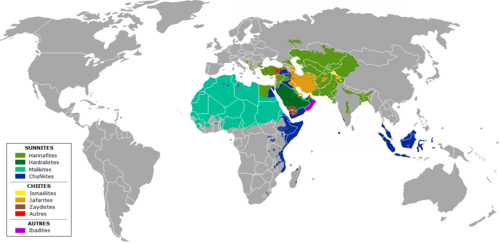
\includegraphics{Images/image097.png}
\vide{ruxe9ponse-soufie}{%
\subsection{Réponse soufie}\label{ruxe9ponse-soufie}}

Je vous propose de lire la lettre du Cheikh Ahmad al-Alawī
(1874-1934)~intitulée «~Lettre ouverte à celui qui critique le
soufisme~».

\vide{v--les-ordres-confruxe9riques}{%
\section{Les ordres
confrériques}\label{v--les-ordres-confruxe9riques}}

Il y en a une cinquantaine dans le monde.

\begin{itemize}
\item
  \textit{La qādirīya} \label{Def:Soufiqādirīya}
Fondateur~: `Abd al-Qādir al-Ğīlānī (m. 1166)
Implantation~: dans tous les pays musulmans, du Maghreb à la Chine


\item
  \textit{La Naqchabandīya} \label{Def:SoufiNaqchabandiya}
Fondée au milieu du XIV° siècle
Implantation~: du Caucasse au Turkestan et à l'Inde
Elle a nourri le nationalisme kurde


\item
  \textit{La Šāḏilīya} \label{Def:Soufisadiliya}
Eric Geoffroy dit de la \emph{Šāḏiliyya} qu'elle est l'une des
«~voies-mères~» du soufisme. Elle est apparue entre la fin du
XII\textsuperscript{e} siècle et le XIV\textsuperscript{e} siècle.
D'origine maghrébine, elle s'est diffusée au XIII\textsuperscript{e}
siècle, à partir de l'Égypte, dans la majeure partie du monde musulman.
Son enseignement est dense et il s'appuie sur les écrits d'Ibn
\emph{`}Arabī.
\end{itemize}
Toute voie initiatique a pour but de mener ses adeptes vers la sainteté,
ou «~proximité divine~» (\emph{walâya})~; celle-ci est identifiée au
plus haut degré de la gnose par al-Shâdhilî. De façon schématique, les
premiers maîtres shâdhilis distinguent deux niveaux~: la sainteté
«~mineure~» (\emph{sughrâ}), ouverte au public large des fidèles, et la
sainteté «~majeure~» (\emph{kubrâ}), réservée à une élite spirituelle.
Mais le terme \emph{walâya}, tout comme celui de sainteté en français,
est un terme générique, un idéal qui implique une méthode pour y
parvenir.

Pour les Shâdhilis, la réponse est claire~: c'est dans l'imitation
intérieure du Prophète que se réalise la \emph{walâya}. Réapparaît ici
le débat millénaire sur les rapports entre \emph{walâya}et
\emph{nubuwwa}, la prophétie, débats qui ont partagé exotéristes et
ésotéristes de l'islam, mais aussi les milieux soufis. Autant les
maîtres shâdhilis initiaux se réclament du premier théoricien de la
sainteté en islam, al-Hakîm al-Tirmidhî (m. 318/930), autant ils s'en
éloignent lorsque celui-ci accorde à la \emph{walâya}une autonomie par
rapport à la \emph{nubuwwa}~: pour eux, la première est subordonnée à la
seconde, et puise sa substance même dans la Lumière muhammadienne
(\emph{al-nûr al-muhammadî}).

\begin{itemize}
\item
  \textit{La Bekt'āchīya}
Elle impose le célibat
De nombreux affiliés en Turquie et Albanie


\item
  \textit{La Tidjānīya}
Influente au Maghreb et dans l'Afrique occidentale


\item
  \textit{La Chattārīya}
Influente en Inde et Malaisie

\item
  \textit{La Rah'mānīya}
La plus influente confrérie algérienne.


\item
  \textit{La mawlāwīya} (derviches)
\end{itemize}

Il existe plusieurs ordres soufis, mais l'on peut distinguer deux grands
groupes de mystiques~: ceux qui se trouvent dans la station de l'ivresse
(\emph{sukr}) et ceux qui sont dans la station de la sobriété
(\emph{sahw}).

Les initiés ivres sont souvent les disciples d'Abū Yazīd Bistamī (m.
875)~: l'ivresse, c'est la perte de sens commun, de la maîtrise de soi.
L'âme est enivrée de la connaissance de Dieu, plongée dans la
contemplation de Dieu.

Pour le second groupe, l'ivresse n'est qu'un état transitoire. Elle est
le début de l'unicité, mais elle se caractérise par la sobriété, quand
il sait que le soi n'est qu'un miroir dans lequel se réfléchit l'Essence
divine.

\paragraph{Pour aller plus loin}

Martin \textsc{Lings}, \emph{Qu'est-ce que le soufisme~?} traduit de
l'anglais par Roger du Pasquier, Paris, Éditions du Seuil, 1977.

Eric \textsc{Geoffroy},
«~\url{http://www.facebook.com/topic.php?uid=21148739744\&topic=3226}{L'islamité
du soufisme et son apport à la spiritualité universelle}~» dans
\url{http://www.religioperennis.org/documents/geoffroy/islamitesoufisme.pdf}

Eric \textsc{Geoffroy}, \emph{Initiation au soufisme}, Coll. L'espace
intérieur, Paris, Fayard, 2003.

Alberto Fabio \textsc{Ambrosio}, \emph{Vie d'un derviche tourneur}.
Doctrine et rituels du soufisme au XVII\textsuperscript{e} siècle,
Paris, CNRS Edition, 2010, 1 vol., 406 pages.

Laleh \textsc{Bakhtiar}, \emph{Le soufisme}. Expressions de la quête
mystique, Paris, Seuil, 1977.

Christian \textsc{Bonaud}, \emph{Le soufisme al-taṣawwuf et la
spiritualité islamique}, Préface de

Michel Chodkiewicz, Maison Larose, IMA, 1991.

\textbf{Exercice pour la Validation}

À partir de la lettre du šaḫy Ahmad al-Alawī, identifierez les éléments
qui répondent aux critiques adressées aux soufis et à Ibn `Arabī tels
que nous les avons exposés.



\chapter{La philosophie en islam}


\section{Introduction
}
\begin{quote}
Un jour, le calife al-Ma'mūn fit un rêve~: «~J'ai vu en rêve un homme
assis dans la posture des sages, je lui ai demandé «~qui es-tu~?~», il
m'a répondu «~Aristote le Sage~». Alors je lui posai la question
«~Dis-moi qu'est-ce que le bien? ~», Aristote de dire : «~ce qui est
conforme à la raison~». Al-Ma'mūn : «~Mais encore~?~», Aristote : «ce
qui est bien selon la révélation~~». Je lui dis : et après ? ~Il me dit
: «~Ce qui est bien aux yeux de tous~». Je lui dis : `et après'. Il me
dit : `il n'y a pas d'après'~Je lui dis : `dis-moi encore autre chose'.
Il me dit : `celui qui te conseille bien au sujet de l'or, qu'il soit
pour toi comme de l'or ; et il te faut reconnaître un Dieu unique'~».
\end{quote}

De ce rêve, supposé reconstruit et visant à justifier le recours à la
philosophie en islam, naquit le projet de créer la Maison de la Sagesse
en 832 qui devint un lieu où de nombreux savants s'attelèrent à traduire
les œuvres de la philosophie grecque\textbf{,} et également \textbf{des}
traités de mathématiques et de médecine. Dimitri Gutas a montré que
cette entreprise de traduction doit être comprise au sein d'un
environnement politique, social et idéologique propre à l'empire
abbasside en quête de légitimité\sn{Dimitri \textsc{Gutas},
  \emph{Pensée grecque, culture arabe : Le mouvement de traduction
  gréco-arabe à Bagdad et la société abbasside primitive
  (IIe-IVe/VIIIe-Xe siècles)}, traduit de l'anglais par Abdessalam
  Cheddadi, Paris, Aubier, 2005.}\textsuperscript{.} Les
descriptions\textbf{,} sous la plume d'auteurs contemporains\textbf{,}
d'une maison de rencontres où se côtoient des juifs, des chrétiens et
des musulmans ressemblent davantage à la projection d'un idéal moderne
qu'à une réalité historique\sn{~À l'exemple de Souleymane Bachir
  \textsc{Diagne}, \emph{Comment philosopher en islam~?}, Paris,
  Panorama, 2008, p. 36. Toutefois, au-delà de représentations
  idéologiques, il est certain que les premiers traducteurs étaient des
  chrétiens issus de milieux jacobites ou nestoriens qui avaient
  préservé dans les bibliothèques de leurs monastères l'essentiel de
  l'héritage aristotélicien. L'assertion d'Alain de Libera, selon
  laquelle la philosophie en terre d'islam a été «~une histoire
  musulmane, cela va sans dire, aussi une histoire chrétienne et une
  histoire juive~»~est bien fondée~: Alain \textsc{de Libera}, \emph{La
  Philosophie médiévale}, Paris, PUF, 1993, p. 54.}. Ce qui prédomine,
ce sont les interactions scientifiques entre philosophes et non des
échanges de théologie. Il reste que la philosophie grecque rencontre
l'univers de l'islam, la \emph{philosophia} devient \emph{falsafa}. Il
s'y affirme l'idée d'une sagesse éternelle (\emph{philosophia perennis})
traversant les âges et les communautés humaines, qu'elles fussent ou non
gratifiées d'une révélation. Cette sagesse {est} transmise grâce
à des hommes comme le «~divin Platon~»\sn{~Al-Ġazālī reprend
  l'expression du «~divin Platon~(Platon \emph{al-ilāhi})~» mais non
  sans ironie~: \textsc{al-Ġazālī}, \emph{Tahāfut al-falāsifa},
  p. 8. {[}Marmuna, p. 4{]}}, sagesse que le croyant ne peut méconnaître
mais qu'il doit au contraire s'approprier. Dans ce foisonnement de
traductions et de rencontres -- Platon, Aristote, Plotin sont ainsi
traduits en arabe dès la fin du IXe siècle, l'élite intellectuelle débat
de questions nouvelles. Les controverses foisonnent entre musulmans et
chrétiens ou juifs, entre sunnites et šī`ites, entre mutazilites et
aš`arites où, derrière un style non dénué d'expressions caustiques,
l'atmosphère y est celle d'une ouverture à l'autre comme en témoigne Abū
Hayyān al-Tawhīdī\sn{Marc \textsc{Berg}É, \emph{Pour un humanisme
  vécu~: Abū Hayyān al-Tawhīdī}, Institut français de Damas, 1979.}.
Munis des outils et des questions de la philosophie grecque, des
penseurs arabes en viennent à élaborer leurs propres systèmes
philosophiques. Trois auteurs occupent une place singulière dans cette
histoire~: al-Kindī (m. 870), al-Fārābī (m. 950) et Ibn Sīnā (m. 1037).
Il s'agit d'Avicenne. Avec al-Fārābī, le \emph{kalām} devient une
science spécifique et les connaissances prophétiques et philosophiques
renvoient à deux modes distincts d'appréhension d'un même objet. Sous
l'influence du néo-platonisme et du milieu šī`ite, al-Fārābī construit
une cosmogonie caractérisée par la procession des intellects au sein
d'un monisme émanatiste\textbf{.} Mais la séparation entre philosophie
et orthodoxie musulmane atteint son paroxysme avec les écrits d'Ibn
Sīnā. La création n'y est plus comprise comme un acte de volonté libre
comme l'affirme le Coran, mais elle relève d'une nécessité propre à
l'être divin. Par ailleurs, Ibn Sīnā déconstruit les dogmes musulmans
par une lecture symbolique qui privilégie le sens ésotérique
(\emph{bāṭin}) et relaie au second plan le sens exotérique
(\emph{ẓāhir}) des versets coraniques. Pour Ibn Sīnā, la résurrection
des corps est de l'ordre de la métaphore et non de la
réalité\sn{~Ibn \textsc{S}Ī\textsc{n}Ā, \emph{Al-Risāla
  al-Aḍḥawiyya}/}.

Les systèmes philosophiques développés par les philosophes arabes ne
manquent pas d'audace et d'originalité pour la pensée musulmane de
l'époque, mais peuvent-ils s'accorder avec l'islam~? Relèvent-ils de
questions périphériques à l'islam ou contredisent-ils l'enseignement de
la révélation coranique~? Relèvent-ils d'une sagesse universelle ou
d'une logique singulière qui ne saurait s'accorder avec la logique
propre à l'arabe, autrement dit, peut-on projeter sur les versets du
Coran une lecture philosophique grecque alors même qu'elle s'oppose à la
logique de la langue arabe qui n'est autre que la grammaire
arabe~?\sn{Allusion ici à la célèbre controverse entre le
  Nestorien Mattā b. Yūnus (m. 328/940) et le musulman al-Sīrāfī.
  Voir~pour l'édition~: Abdelali \textsc{Elamrani-Jamal}, \emph{Logique
  aristotélicienne et grammaire arabe}, Paris, Vrin, 1983. Voir
  aussi~David Samuel \textsc{Margoliouth}, «~The discussion between Abu
  Bishr Matta and Abu Saʿid al-Sirafī on the merits of logic and
  grammar~», dans \emph{Journal of the royal Asiatic society}, London,
  1905, p. 79-129.} Questions éminemment redoutables, questions toujours
modernes. Pour autant, initialement et contrairement à l'Occident, le
débat ne porte pas tant sur l'opposition entre la foi et la raison que
sur celle entre la religion officielle et un système philosophique.


\section{Logique grecque et logique islamique~:
débats autour de la langue
}


\subsection{1.1 le statut de la langue
arabe}

La philosophie se dit en arabe \emph{falsafa} et les philosophes se
nomment \emph{falāsifa}. Par cette désignation se trouve clairement
indiquée l'origine grecque de cette discipline. Elle se situe en dehors
des sciences traditionnelles de l'islam. Si l'interrogation est
indépendante en soi de l'appartenance religieuse, dans quelle mesure y
a-t-il eu une appropriation de la pensée grecque par l'islam~? Dans
quelle mesure y a-t-il eu une islamisation de cette pensée~? Mais aussi,
en recourant au grec, la pensée musulmane ne s'est-elle pas hellénisée~?
Dans ce cas, n'y a-t-il pas risque de voir trahi le message originel de
la révélation donné en arabe~?

En effet, le Coran en ses versets de la sourate 41, 2-3 fait mention
explicite~de l'arabe comme langue de la révélation coranique :
\begin{quote}
    «~C'est
une révélation descendue de la part du Tout Miséricordieux, du Très
Miséricordieux. Un Livre dont les versets sont détaillés, un Coran arabe
pour des gens qui savent~»
\end{quote}.
Cette expression a été comprise de deux
manières~:

\begin{itemize}
\item
  l'arabe est une langue sacrée, la langue choisie pour dire la parole
  de Dieu, langue de Dieu.
\item
  L'arabe est une langue humaine, elle n'est qu'humaine. Chaque messager
  a reçu un message dans la langue de son peuple~: «~Nous n'avons envoyé
  de messager qu'avec la langue de son peuple, afin de les éclairer~»
  (S. 14,4). Ainsi, s'il y a une langue du Coran, il n'y a pas pour
  autant une langue de l'islam.
\end{itemize}

Pour les partisans de la première interprétation, l'arabe comme langue
de Dieu, comme langue sacrée, ne saurait subir l'introduction d'un
vocabulaire étranger sans perdre sa pureté. Les mots étrangers en
altérant la langue altèrent l'islam même. Ici, la \emph{falsafa} est
montrée du doigt et bannie. Ce débat renvoie à une controverse fameuse
entre Mattā Ibn Yūnus et al-Sīrāfī.


\subsection{La controverse entre Mattā Ibn Yūnus et
al-Sīrāfī
}
Mattā est un chrétien nestorien et al-Sīrāfī est un grammairien
musulman. Entre eux deux s'est tenue une controverse très animée et
polémique.

Sīrāfī, en effet, dénonce les prétentions de la logique grecque à
s'immiscer dans la langue arabe. Or, elle ne saurait y trouver accueil
et hospitalité~! L'animosité est aussi confessionnelle puisque Mattā est
chrétien. Il est l'exemple même de la dérive possible due aux religions
étrangères. Sīrāfī entend donc ridiculiser son adversaire. Il lui pose
des colles comme pour montrer son incompétence en arabe et pour
l'empêcher de développer ses thèses. Pourtant, Mattā veut montrer qu'une
vérité universelle peut être traduite dans d'autres idiomes, et que
c'est cette possibilité qui définit le vrai. Les intelligibles sont les
mêmes, quels que soient les langues dans lesquelles ils se disent~: «~ne
vois-tu pas que 4+4 font huit, qu'ils font toujours 8 en grec comme en
arabe~! » lance-t-il à al-Sīrāfī. Mattā défend donc la thèse d'une
vérité universelle contre le relativisme linguistique de Sīrāfī. Pour
Sīrāfī, chaque langue est un monde à part, avec une logique propre,
spécifique. Il n'y a pas de grammaire générale mais seulement des
grammaires particulières. Il n'y a pas de grammaire philosophique, il y
a une logique grecque et il y a une logique arabe laquelle n'est autre
que la grammaire arabe. Traduire la logique grecque en arabe, c'est donc
trahir la logique arabe et donc la Révélation.

Ce débat est d'une étonnante modernité, que l'on songe à toute la
difficulté de la notion d'être qui n'existe pas dans certaines langues,
et qui est une catégorie métaphysique grecque.

Mais derrière des enjeux linguistiques et techniques se joue celui de
l'ouverture à l'autre. Al-Sīrāfī est pour une exégèse de la révélation
qui n'utilise pas les catégories dialectiques de la Grèce. Mattā est
pour le contraire. Il veut que l'arabe devienne aussi une langue de la
philosophie.


\section{La philosophie islamique
}


\subsection{Définition
}
Le titre de ce chapitre «~la philosophie en islam~» pose une certaine
difficulté En effet, ne faut-il pas parler de philosophie arabe~? Dans
ce cas, cela inclurait les chrétiens et les juifs qui s'expriment en
arabe. Faut-il plutôt parler de philosophie islamique de langue arabe~?
Mais que faire d'al-Ġazālī \label{theol:AlGazali26} qui s'est exprimé en arabe et en
persan\ldots~? Pour le professeur Rémi Brague, il n'y a pas de
philosophie islamique. Il n'y a qu'un usage de pensées philosophiques de
la part des musulmans. La philosophie a été pratiquée par des musulmans.

Le philosophe Suleyman Diagne propose cependant de définir la
philosophie islamique comme étant la relecture des récits de la
tradition islamique à la lumière de la raison.


\subsection{Illustration~: le Commentaire d'Avicenne
sur le voyage nocturne de Muḥammad
}

\subsubsection{Récit du voyage
nocturne}

Il en est question dans le Coran et dans la Sira.

Dans le Coran, on en trouve~mention aux sourates 17\textsuperscript{ème}
et 53\textsuperscript{ème}.

S. 17,1~: Gloire et Pureté à Celui qui de nuit, fit voyager Son
serviteur {[}Muhammad{]}, de la Mosquée Al-Haram à la Mosquée Al-Aqsa
dont Nous avons béni les alentours, afin de lui faire voir certaines de
Nos merveilles. C'est Lui, vraiment, qui est l'Audient, le
Clairvoyant\sn{S. 17, 1

  \TArabe{سُبْحَانَ الَّذِي أَسْرَى بِعَبْدِهِ لَيْلاً مِّنَ الْمَسْجِدِ
  الْحَرَامِ إِلَى الْمَسْجِدِ الأَقْصَى الَّذِي بَارَكْنَا حَوْلَهُ
  لِنُرِيَهُ مِنْ آيَاتِنَا إِنَّهُ هُوَ السَّمِيعُ البَصِيرُ}}.

Dans la S. 53, il est question d'une rencontre, d'une ascension depuis
Jérusalem jusqu'au Lotus de la Limite. Il a vu alors les merveilles de
son Seigneur.

Mais ce sont surtout les \emph{ḥadīṯs} qui donnent les détails les plus
nombreux de ce voyage. Ils sont compilés par al-Buḫārī et
Muslim\sn{Traduit de l'arabe du livre de Sheikh Yâsîn Rushdî,
  \emph{Fî Ri\underline{h}âb Al-Mu\underline{st}afâ} (En Compagnie de
  l'Élu), disponible sur le site
  \url{http://www.mouassa.org/Arabic/FiRehab/index.htm}.
  traduction non revue et consultable sur le site
  \url{http://www.islamophile.org/spip/Le-Voyage-Nocturne-et-l-Ascension,1368.html}
}.

\begin{quote}
Au sujet du Voyage Nocturne, le Prophète --- paix et bénédictions sur
lui --- dit~: «~Le plafond de ma maison s'ouvrit alors que j'étais à La
Mecque. Jibrîl descendit, il ouvrit ma poitrine et la lava à l'eau de
Zamzam. Puis il apporta une bassine en or, emplie de sagesse et de foi,
qu'il vida dans ma poitrine, puis il la referma. Ensuite, on m'apporta
le Burâq~; il s'agit d'une bête blanche élancée, entre l'âne et le
mulet, qui pose son sabot à perte de vue. Je l'enfourchai et arrivai à
la Mosquée de Jérusalem. Je l'attachai à l'anneau que les prophètes
emploient à cet effet, puis j'entrai dans la Mosquée.~»~
Al-\underline{H}asan --- que Dieu l'agrée --- de poursuivre~: «~Il y
trouva Abraham, Moïse et Jésus dans une assemblée de prophètes. Alors,
le Messager de Dieu fut leur imam dans une prière qu'ils accomplirent en
congrégation. Puis, on apporta deux récipients, l'un contenant du vin,
l'autre du lait.~» Il poursuivit~: «~Le Messager de Dieu prit celui qui
contenait du lait et en but. Il laissa celui qui contenait du vin.~» Il
poursuivit~: «~Alors Jibrîl lui annonça~: ``Tu as été guidé vers la
nature primordiale (\emph{fi\underline{t}rah}) et ta communauté a été
guidée, ô Mu\underline{h}ammad. Le vin vous a été défendu.'' Puis le
Messager de Dieu retourna à la Mecque. Le lendemain matin, il relata cet
événement aux gens de Quraysh.

Le Prophète dit~: «~Puis Jibrîl vint avec le \emph{Mi`râj} Puis nous
montâmes au ciel. Alors Jibrîl demanda l'accès. On lui dit~: ``Qui
es-tu~?'' Il répondit~: ``Jibrîl''. On s'enquit~: ``Qui est avec toi~?''
Il répondit~: ``Mu\underline{h}ammad''. On demanda~: ``Fut-il investi de
sa mission prophétique~?'' Il dit~: ``Oui, il en fut investi''. On nous
ouvrit et je vis alors Adam qui m'accueillit chaleureusement et fit des
invocations en ma faveur.

Puis nous montâmes au deuxième ciel et Jibrîl demanda l'ouverture du
ciel. On lui dit~: ``Qui es-tu~?'' Il répondit~: ``Jibrîl.'' On
s'enquit~: ``Qui est avec toi~?'' Il répondit~:
``Mu\underline{h}ammad.'' On demanda~: ``Fut-il investi de sa mission
prophétique~?'' Il dit~: ``Oui, il en fut investi.'' On nous ouvrit et
je vis alors les deux cousins maternels --- Jésus (`Îsâ), le fils de
Marie, et Jean-Baptiste (Ya\underline{h}yâ), le fils de Zacharie ---
paix et bénédictions sur eux ---. Ils m'accueillirent chaleureusement et
firent des invocations en ma faveur.

Puis nous montâmes au troisième ciel. Alors Jibrîl demanda l'accès. On
lui dit~: ``Qui es-tu~?'' Il répondit~: ``Jibrîl.'' On s'enquit~: ``Qui
est avec toi~?'' Il répondit~: ``Mu\underline{h}ammad.'' On demanda~:
``Fut-il investi de sa mission prophétique~?'' Il dit~: ``Oui, il en fut
investi.'' On nous ouvrit et je vis alors Joseph --- paix et
bénédictions sur lui --- qui, à lui seul, avait reçu la moitié de la
beauté. Il m'accueillit chaleureusement et fit des invocations en ma
faveur.

Puis nous montâmes au quatrième ciel. Alors Jibrîl demanda l'accès. On
lui dit~: ``Qui es-tu~?'' Il répondit~: ``Jibrîl.'' On s'enquit~: ``Qui
est avec toi~?'' Il répondit~: ``Mu\underline{h}ammad.'' On demanda~:
``Fut-il investi de sa mission prophétique~?'' Il dit~: ``Oui, il en fut
investi.'' On nous ouvrit et je vis alors Idrîs --- paix et bénédictions
sur lui --- qui m'accueillit chaleureusement et fit des invocations en
ma faveur. Dieu dit à son sujet~: ``Nous l'élevâmes à un haut rang.''

Puis nous montâmes au cinquième ciel. Alors Jibrîl demanda l'accès. On
lui dit~: ``Qui es-tu~?'' Il répondit~: ``Jibrîl.'' On s'enquit~: ``Qui
est avec toi~?'' Il répondit~: ``Mu\underline{h}ammad.'' On demanda~:
``Fut-il investi de sa mission prophétique~?'' Il dit~: ``Oui, il en fut
investi.'' On nous ouvrit et je vis alors Aaron --- paix et bénédictions
sur lui --- qui m'accueillit chaleureusement et fit des invocations en
ma faveur.

Puis nous montâmes au sixième ciel. Alors Jibrîl demanda l'accès. On lui
dit~: ``Qui es-tu~?'' Il répondit~: ``Jibrîl.'' On s'enquit~: ``Qui est
avec toi~?'' Il répondit~: ``Mu\underline{h}ammad.'' On demanda~:
``Fut-il investi de sa mission prophétique~?'' Il dit~: ``Oui, il en fut
investi.'' On nous ouvrit et je vis alors Moïse --- paix et bénédictions
sur lui --- qui m'accueillit chaleureusement et fit des invocations en
ma faveur.

Puis nous montâmes au septième ciel. Alors Jibrîl demanda l'accès. On
lui dit~: ``Qui es-tu~?'' Il répondit~: ``Jibrîl.'' On s'enquit~: ``Qui
est avec toi~?'' Il répondit~: ``Mu\underline{h}ammad.'' On demanda~:
``Fut-il investi de sa mission prophétique~?'' Il dit~: ``Oui, il en fut
investi.'' On nous ouvrit et je vis alors Abraham qui était adossé au
Temple Peuplé (\emph{Al-Bayt Al-Ma`mûr}). Chaque jour soixante-dix
milles anges y pénètrent et n'y retournent guère. Puis il m'emmena à
\emph{Sidrat Al-Muntahâ} (Arbre de l'Aboutissement). Ces feuilles
étaient grandes comme des oreilles d'éléphant et ses fruits étaient
comme des amphores. Mais par un ordre divin, il se transforma si bien
que nulle créature ne pouvait le décrire tant il était beau. Alors Dieu
me révéla ce qu'Il me révéla, et me prescrivit cinquante prières
quotidiennes. Puis je descendis vers Moïse qui me demanda~: ``Quelle
prescription Dieu a-t-il imposé à ta communauté~?'' Je lui dis~:
``Cinquante prières.'' Alors il dit~: ``Retourne voir ton Seigneur, et
demande lui un allégement, car ta communauté ne pourra le supporter~;
j'ai éprouvé les Fils d'Israël et j'ai vu ce qu'il en était.'' Je
retournai ainsi vers mon Seigneur et lui dis~: ``Seigneur~! Allège ce
que Tu as demandé à ma communauté.'' Alors, il réduisit de cinq le
nombre de prières. J'allai voir Moïse et lui dis~: Il les a réduites de
cinq prières. Alors il me dit~: ``Ta communauté ne pourra supporter
cela, retourne vers ton Seigneur, et demande lui un allégement
supplémentaire.'' Je ne cessai d'aller voir mon Seigneur --- Exalté
soit-Il --- puis de retourner à Moïse, jusqu'à ce qu'Il me dise~:
«~Mu\underline{h}ammad, cinq prières quotidiennes sont prescrites.
Chacune en vaut dix~; elles valent ainsi cinquante prières. De plus,
quiconque a l'intention de faire une œuvre pie, s'il ne l'accomplit pas,
il recevra une rétribution simple et s'il l'accomplit il en recevra dix.
Et quiconque a l'intention de commettre une mauvaise œuvre et s'en
abstient, elle ne sera point comptée à son détriment~; mais, s'il la
commet, elle comptera pour une seule mauvaise action.~» Quand je vins à
Moïse, il me dit~: ``Retourne voir ton Seigneur, et demande lui un
allégement.'' Je répondis~: ``Je n'ai cessé d'aller voir mon Seigneur à
ce sujet au point d'en être
embarrassé.''~»

Les gens divergèrent également sur la question de savoir si le Prophète
--- paix et bénédictions sur lui --- vit son Seigneur ou non. À ce
sujet, citons les narrations les plus authentiques.
\end{quote}


\subsubsection{Une lecture
philosophique}

C'est un récit qui fait appel à l'imagination, récit chargé d'images, de
merveilleux. Mais au-delà de ces images la tâche du philosophe est de
les interpréter selon la raison.

Or, Avicenne dans son Livre \emph{Miraj Nama}, \emph{Le livre de
l'Ascension}, s'applique à donner une lecture rationnelle de ce récit.


\subsubsection{
Avicenne}

Son nom est Abū Ali al-Hussayn Ibn `Abdallah Ibn Sīnā.

Il est d'origine persane. Né en 980 près de Boukhara (Ouzbékistan
actuel). Il vit dans un contexte d'une grande instalbilité politique. Il
a appris les sciences du Coran. Il est déoué d'une mémoire prodigieuse
au point qu'il a mémorisé l'ensemble du Coran à l'âge de 10 ans. Son
génie se manifeste en médecine. À l'âge de 17 ans, il parvient à guérir
un prince musulman de sa maladie. En guise de remerciement, le prince
ouvre au jeune étudiant sa bibliothèque, ce qui lui permettra d'acquérir
un savoir encyclopédique. Il lit 40 fois la \emph{Métaphysique}
d'Aristote. Un commentaire d'al-Fārābī, autre philosophe musulman, lui
en donne les clefs. On l'appelle le troisième Maître après Aristote et
al-Fārābī.

Ses ouvrages les plus célèbres sont~: \emph{Le livre de la guérison},
\emph{al-Šifā'}, et \emph{Le canon de la médecine}. Il a écrit une
centaine d'autres ouvrages, parmi lesquels une réfutation de
l'astrologie~: s'il juge les outils scientifiques, ses principes ne le
sont pas.

Ibn Sīnā était excellent mathématicien, mais s'il a été novateur en
médecine et philosophie, il n'a pas été novateur en mathématique. En
revanche, il comprenait ce qui se découvrait en mathématique. Pour lui,
l'usage de la raison n'est pas en opposition avec la foi religieuse.

En philosophie, il a une conception de l'universel~(\emph{kull}) ; il
généralise le terme de \emph{šay'}~: les choses peuvent ne pas être
existantes~; il distingue entre l'existence et l'essence. Pour lui,
l'existence s'ajoute à l'essence sauf dans le cas de Dieu où essence et
existence sont indistincts car Dieu est \emph{ṣamād}, impénétrable~; la
plénitude divine fait que l'existence ne peut pas s'y ajouter.

Il connut des épreuves et dut fuir à travers la Transoxiane et la Perse.
Il connut la prison pour être rentré en contact avec un prince rival. Il
meurt en 1037.

Ibn Sīnā est le produit d'une société qui a connut une dynamique
d'assimilation des traductions et de créativité. Son aura est d'abord
médicale~: Le canon de la médecine est une encyclopédie médicale. Il y
traite des instruments de chirurgie, d'anatomie, de la circulation du
sang. Il décrit plus de 700 médicaments qu'il invite à tester sur les
animaux. Il souligne aussi les effets de la musique et de ses incidences
bénéfiques pour le malade. Il démontre que la contagion a lieu par
l'eau. Ce canon est à la fois la synthèse de la médecine antique mais
aussi le fruit de ses observations personnelles. Jusqu'au
17\textsuperscript{ème} siècle, son livre sera la référence de tous les
étudiants en médecine en Europe.

Avicenne se démarque dans les domaines de l'ophtalmologie, de la
gynéco-obstétrique et de la psychologie. Il s'attache beaucoup à la
description des symptômes, décrivant toutes les maladies répertoriées à
l'époque, y compris celles relevant de la psychiatrie.

Mais avant tout, Avicenne s'intéresse aux moyens de conserver la santé.
Il recommande la pratique régulière du sport et préconise une médecine
préventive et curative. Il insiste sur l'importance des relations
humaines dans la conservation d'une bonne santé mentale et somatique. En
s'appuyant sur la logique, il propose de guérir par les contraires, idée
de la dialectique aristotélicienne. C'est ici son innovation médicale
majeure. Il y a une fécondation par des savoirs qui étaient isolés. Pour
lui, 
\begin{quote}
    
\emph{«~}la médecine est l'art de conserver la santé et
éventuellement, de guérir la maladie survenue dans le corps\emph{~».}

\end{quote}
Une des grandes innovations de cet ouvrage est son «~architecture~»,
avec une mise en ordre des savoirs de la médecine, et l'intégration des
apports de Rāzī ou Gallien dans une conception renouvelée de la
médecine.

 
\subsubsection{Une pensée émanatiste
}

Pour Avicenne, la pensée divine produit une succession d'Intelligences
(les anges) qui veillent sur nous. Ce sont ces Intelligences qui
éclairent l'intelligence humaine et nous permettent de comprendre les
réalités intelligibles~comme la lumière nous permet de voir les choses
sensibles. Notre intelligence devient active grâce à l'effusion de
l'Intellect agent dont la source est divine.

Mais en l'homme se trouve une faculté végétative et sensitive. Comme
tout procède de Dieu, tout désire retourner à Dieu. Ce désir en l'homme
est tourné vers Dieu. Et pour Avicenne, c'est ce désir qui arrache le
Prophète à son sommeil. Il est amené à la mosquée sacrée qui est le
centre de ce monde-ci et donc la porte qui ouvre sur l'autre monde.


\subsubsection{La nature humaine dans le Livre
de l'Ascension}

L'Avertissement est clair~: il s'agit de répondre à ceux qui
s'enquièrent d'une explication rationnelle. Pas de conte, pas de
merveilleux. Il ne sert à rien de divulguer les secrets à une personne
qui ne peut les entendre. Pire, c'est une faute. En revanche, à celle
qui peut les entendre, c'est un devoir de le faire.

La première partie parle de la nature humaine~: elle est composée de
deux entités différentes~: le corps et l'esprit. L'union du corps et de
l'esprit est comme celle du cavalier et de sa monture.

Il y a dans le corps trois types d'âme~: la naturelle connectée au foie,
l'animale reliée au cœur, la rationnelle reliée au cerveau. Les deux
premières doivent servir la troisième~: c'est ce degré de service qui
différencie les hommes entre eux. Tout dépend donc de la domination
exercée par telle ou telle âme.

L'âme rationnelle dirige, ordonne, sous la supervision de l'intelligence
appelée aussi esprit~; c'est la faculté la plus haute qui est fixée sur
l'Intelligence agente.

L'humain a le désir de se réaliser dans la plénitude qui le conduit vers
le plaisir. Ce plaisir plein est celui que procure l'intelligence des
choses intelligibles. Sa recherche ne s'arrête pas à une ascension vers
soi-même. L'intellect qui est le centre de notre humanité est aussi une
ouverture sur toutes les intelligences émanées de Dieu. Dès lors que
l'on est en contact avec telle ou telle intelligence, cela engendre en
nous une connaissance, une attitude. Celui qui est uni à la Première
Intelligence émanée, Intelligence universelle, acquiert une
compréhension universelle. Son intellect devient alors prophétique.

Cette description de la nature humaine n'est pas un préalable au voyage
nocturne de Muḥammad. Elle est son explication. L'ascension est
l'accession de l'homme à ce qu'il est et à ce qu'il doit devenir.



\subsubsection{Commentaire du
Voyage}

\begin{itemize}
\item
  Le prophète se trouvait dans un état de veille~: il faut le silence
  des sens, de la faculté irascible et de l'imagination pour commencer à
  s'éveiller spirituellement. Le désir du vrai nécessite donc ce
  silence, ce sommeil.
\item
  L'arrivée de Gabriel~: c'est l'Intelligence émanée, l'Esprit Saint,
  qui éclaire l'intellect humain et lui transmet le commandement de
  Dieu.
\item
  Avicenne fait mention de l'enlacement du prophète par l'ange qui se
  présente comme son frère~et qui l'embrasse : cela traduit la
  compénétration de l'intellect humain et de l'Esprit Saint.
\item
  Al-Bourakh~: le coursier ailé entre l'âne et la mule~: cette hybridité
  traduit la faculté de l'Esprit Saint d'être un intermédiaire entre
  l'intelligence humaine et l'Intelligence universelle. Cet Esprit Saint
  a la faculté de transporter l'intellect humain vers des réalités
  spirituelles pour lesquelles il est fait.
\item
  Le choix entre le lait et le vin~: dans cette ascension, les appétits
  tirent vers le bas
\item
  Tous les prophètes sont autant d'intelligences.
\item
  La rencontre avec Dieu~par laquelle on devient prophète. Mais être
  prophète, ce n'est pas s'anéantir dans l'ineffable, s'unir
  mystiquement à lui. C'est revenir aux autres pour s'adresser aux
  humains. Un prophète doit redescendre de la montagne pour parler aux
  humains. Mais le langage humain se heurte à celui du langage divin. Il
  convient donc de mettre en image, par la faculté imaginative. Les
  images traduisent l'expérience de la vérité. Elles parlent à tous~: à
  ceux qui s'arrêtent à la lettre, comme à ceux qui remontent à son
  esprit.
\end{itemize}

On voit ici ce que philosophie islamique peut signifier~: il ne s'agit
pas seulement de traduire un texte grec en arabe et de le commenter,
mais il s'agit de lire un récit islamique à la lumière du \emph{De
anima} d'Aristote. Pour les orthodoxes, cette démarche est indue.
L'islam n'a que faire de la philosophie païenne, elle crée même une
distorsion, une déviation. Elle contribue même à introduire des idées
pernicieuses et contraires à la foi.

Dans la tradition musulmane, celui qui est perçu comme le plus grand
contradicteur de la philosophie islamique porte le nom d'al-Ġazālī  \label{theol:AlGazali2}. Il
semblerait qu'après sa critique, il ne peut plus y avoir de philosophie
en islam. Voyons de plus prêt.

\hypertarget{la-critique-dal-ux121azux101lux12b-de-la-philosophie}{%
\section{3. La critique d'al-Ġazālī de la
philosophie}\label{la-critique-dal-ux121azux101lux12b-de-la-philosophie}}

Le \emph{Tahāfut al-falāsifa} est indéniablement l'ouvrage où al-Ġazālī \label{theol:AlGazali3}
expose la critique la plus rigoureuse et la plus systématique des thèses
philosophiques qui ont cours à son époque.

Les prolégomènes et l'épilogue à l'ouvrage mettent en lumière le lien
entre la mécréance (\emph{kufr}) et l'adhésion à ces doctrines
philosophiques qui relèvent pour al-Ġazālī de l'ordre du credo
(\emph{`aqīda}). Ainsi, après avoir demandé à Dieu de le préserver des
flambeaux de l'obscurité dans une apostrophe sublime, al-Ġazālī dénonce
l'impiété d'un groupe de personnes (\emph{ṭā'ifa}) parmi les musulmans
dont les sentiments de supériorité et d'acuité intellectuelle les ont
conduit à s'éloigner des hommes pieux, à «~mépriser les cérémonies de la
religion, les divisions de la prière, la crainte du péché, {[}à{]} se
railler des prescriptions de la loi et de ses limitations~»\sn{\textsc{al-Ġazālī},
  \emph{Tahāfut al-falāsifa}, \emph{op. cit}., p. 4, {[}Marmuna, p.
  1{]}. Nous reprenons ici la traduction du B\textsuperscript{on}
  \textsc{Carra de Vaux}, p. 146.}. Citant le Coran, ils sont pour
al-Ġazālī de ceux qui «~détournent de la voie de Dieu, qui cherchent à
la rendre tortueuse et qui au dernier jour feront partie des
incroyants~(\emph{kāfirīna}) (S. 11, 19)~»\sn{\textsc{al-Ġazālī},
  \emph{Tahāfut al-falāsifa}, \emph{op. cit.,} p. 4, {[}Marmuna, p.
  2{]}.}. La source de leur incroyance (\emph{maṣdar kufrihum}) est à la
fois religieuse et morale~: ils ont en effet délaissé la certitude de la
religion de leurs pères d'une manière insouciante en prêtant l'oreille à
la nouveauté des opinions, en suivant «~les gens de l'innovation et les
esclaves des passions (\emph{ahl al-bida`} \emph{wa
al-ahwā'})~»\sn{\textsc{al-Ġazālī}, \label{theol:AlGazali3} \emph{Tahāfut
  al-falāsifa}, \emph{op. cit}., p. 4, {[}Marmuna, p. 2{]}.}. Afin de
donner une caution intellectuelle à leur posture immorale, leurs meneurs
prirent appui sur les noms honorables des philosophes grecs tels
Socrate, Hippocrate, Platon ou Aristote. Forts de cette assise
philosophique, ils sont persuadés de pouvoir scruter la profondeur des
choses cachées (\emph{al-'umūr al-ḫafiyya}). Or, font-ils remarquer, ces
philosophes, éclairés par leur savoir, niaient la loi et les religions.
Il convient donc de les imiter.

D'emblée, remarquons qu'al-Ġazālī \label{theol:AlGazali4} ne nie pas la beauté des principes de
la philosophie antique, la qualité et la précision de leur logique, de
leur géométrie ou de leur physique, mais il voit dans le recours à ces
philosophes une nouvelle forme d'imitation (\emph{taqlīd}) qui vient se
substituer à la transmission traditionnelle de la foi. Or, cet abandon
de la connaissance de Dieu au profit de l'imitation d'esprits impies,
sous couvert d'intelligence et d'habileté, est pour lui pure
transgression et démence~(\emph{ḫarq wa ḫabāl})\sn{\textsc{al-Ġazālī},
  \emph{Tahāfut al-falāsifa}, \emph{op. cit}., p. 5, {[}Marmuna, p.
  2{]}.}. En outre, al-Ġazālī relève que non contents d'épouser ces
idées, ces pseudo-philosophes accusent de sottise et d'illusion la
répugnance qu'éprouvent les serviteurs de Dieu à changer leurs
croyances.

Devant ce constat de crise, de dénigrement condescendant mais aussi de
contagion, al-Ġazālī  \label{theol:AlGazali5} entreprend la réfutation (\emph{radd}) des
philosophes pour montrer «~l'incohérence de leurs croyances et la
contradiction de leur discours (\emph{tanāquḍ kalimatihim}) en ce qui
concerne la métaphysique~(\emph{al-ilāhiyyāt})~»\sn{\textsc{al-Ġazālī},
  \emph{Tahāfut al-falāsifa}, \emph{op. cit}., p. 6, {[}Marmuna, p.
  3{]}.}.

L'intention première d'al-Ġazālī, telle qu'elle transparaît dans ces
prolégomènes, n'est donc pas de combattre les philosophes, mais plutôt
ceux qui se réclament des philosophes et s'appuient sur eux pour
s'écarter de l'islam, tout en voulant justifier et fonder
rationnellement leur conduite. Il est symptomatique à cet égard
qu'al-Ġazālī n'expose pas le système d'un philosophe en particulier,
mais plutôt des thèses qui ont court en philosophie. À l'exception d'Ibn
Sīnā, cité quinze fois, d'al-Fārābī, cité deux fois et de quelques
philosophes grecs, al-Ġazālī \label{theol:AlGazali6} ne nomme pas explicitement les philosophes.
Il en expose seulement les idées. Par suite, il n'accuse pas
nominalement d'infidélité ceux qui suivent ces thèses, mais il soutient
que l'affirmation de telle thèse philosophique relève de l'incroyance~:

\begin{quote}
«~Tous les écrits de ces philosophes s'accordent dans la foi en Dieu et
au dernier jour. Toutes les thèses en discussion se ramènent pour moi,
écrit al-Ġazālī, à des écarts à partir de ces deux pôles de la foi, pour
l'affermissement desquels ont été envoyés les prophètes, armés de
miracles. Personne ne songe à les nier, sauf un petit noyau d'hommes à
l'esprit perverti et à la raison renversée, dont on ne s'occupe pas et
qu'on ne cite pas parmi les spéculatifs, mais qui ne peuvent être
comptés que dans la bande des mauvais démons, dans la tourbe des
grossiers et des sots~»\sn{\textsc{al-Ġazālī},
  \emph{Tahāfut al-falāsifa}, \emph{op. cit}., p. 6-7, {[}Marmuna, p.
  3{]}, traduction du B\textsuperscript{on} \textsc{Carra de Vaux,} p.
  148.}.
\end{quote}

Al-Ġazālī \label{theol:AlGazali7}  n'accuse pas les philosophes en général d'impiété. Au
contraire, il affirme qu'ils croient en Dieu et en ses messagers.
Cependant, «~ils s'égarent sur des détails qui suivent les principes
(\emph{fa innahum} \emph{iḫtabaṭū fī tafāṣīl ba`d haḏihi
al-uṣūl})~entraînant une certaine confusion »\sn{\textsc{al-Ġazālī},
  \emph{Tahāfut al-falāsifa}, \emph{op. cit}., p. 7, {[}Marmuna, p.
  3{]}.} pouvant conduire les esprits hors du droit chemin, celui de
l'islam. Dans l'introduction au \emph{Tahāfut}, al-Ġazālī pose donc la
distinction entre les philosophes qui ont foi en Dieu et en ses
messagers et ceux qui ne croient pas. Les premiers peuvent adhérer à des
idées qui ne sont pas celles des croyants de la tradition, mais ils
restent du même avis sur les fondamentaux de la foi. En revanche, ils
peuvent être récupérés par les seconds dont l'esprit «~pervers~» est en
quête de distinction ou d'autojustification.


\section{Conclusion}\

En réponse à al-Ġazālī \label{theol:AlGazali8}, Averroès a rédigé un \emph{Tahāfut al-tahāfut}
c'est-à-dire l'Incohérence de l'Incohérence. Il répond à al-Ġazālī \label{theol:AlGazali25}~:
dans un premier temps, il reconnaît que les critiques philosophiques
d'al-Ġazālī ne sont pas sans justesse. Mais le maître est lui-même
critiquable et c'est ce qu'il entreprend de démontrer dans cet ouvrage.

Je noterai que, contrairement à une idée reçue, al-Ġazālī n'est pas
contre les philosophes. Il rejette certaines de leurs thèses contraires
à la foi, mais lui-même était philosophe. Revenir aux fondations de la
philosophie en islam, renouer avec les anciens, avec leur méthode, leur
épistémologie est sans aucun doute une piste pour l'islam contemporain
en quête de réforme. Car si bien des musulmans appellent à refonder la
pensée musulmane, le grand problème posé porte sur le comment. Comment
s'y prend-t-on~? Ici, la philosophie ouvre des voies qui permettent une
distance aux textes et leur donnent une intelligence.


\section{Bibliographie}


Rémi \textsc{Brague}, «~En quoi la philosophie islamique est-elle
islamique ?~» dans : Geneviève Gobillot, Marie-Thérèse Urvoy,
\emph{L'Orient chrétien dans l'empire musulman : hommage au professeur
Gérard Troupeau}, Paris, Edition de Paris, 2005, p. 119-141.

Souleymane Bachir \textsc{Diagne}, «~Islam et philosophie~: leçons d'une
rencontre~», dans \emph{Diogène}, 2003/2, n° 202, p. 145-151.

A\textsc{l-Ghaz}Ā\textsc{l}Ī, \emph{The Incoherence of the
Philosophers}, \emph{Tahāfut al-falāsifa}, A parallel English-Arabic
text translated, introduced, and annotated by Michael E. Marmura,
Islamic Translation Series, Brigham Young University Press, Provo, Utah,
2000² (1997).

Léon \textsc{Gauthier}, \emph{Ibn Thofaīl, sa vie, ses œuvres}, Paris,
Vrin, 1983.

Peter \textsc{Heath},\emph{Allegory
and Philosophy in Avicenna: With a Translation of the Book of the
Prophet Muhammad's Ascent to Heaven}, University of Pennsylvania Press,
1992.

Jean-Michel \textsc{Hirt}, \emph{Le voyageur nocturne}, Lire à l'infini
le Coran, Paris, Bayard, 2010.

Ibn \textsc{Tufayl}, \emph{Le Philosophe autodidacte}, Paris, Mille et
une nuit, 1999.

\chapter{Eschatologie musulmane}

La question eschatologique est fondamentale. Rappelez-vous, Muḥammad a
commencé la transmission des sourates avec cet appel à la conversion car
la fin des temps est proche. Nous y consacrerons un chapitre. Mais que
se passe-t-il après la mort~? Quelle est donc la théologie des fins
dernières de l'islam~?

Notons d'ores et déjà que les Traités d'eschatologie musulmane à
l'exemple du \emph{Livre de la mort et de l'au-delà}, d'al-Ġazālī
distinguent plusieurs étapes~: celle du Jour de la Résurrection, celle
du Jour Grand Rassemblement, celle du Jour du Jugement. On y décrit
l'enfer, le paradis, mais aussi un lieu étrange~: \emph{al-a`rāf}, sorte
de lieu transitoire.


\subsection{Bibliographie}

Emilio \textsc{Platti}, \emph{Islam\ldots{} étrange~?}, Paris Cerf, p.
65-71.

Sur la résurrection en islam~: l'article de Maurice \textsc{Borrmans},
«~Resurrection~», dans Jane Dammen \textsc{McAuliffe} (ed.)
\emph{Encyclopedia of the Qur'ân}, Leiden, Boston, Brill, 2004,
p.434-435 est une très bonne synthèse pour la dimension coranique. À
noter la récente réédition du classique, paru initialement en 1981, de
Jane Idleman \textsc{Smith}, Yvonne \textsc{Yazbeck Haddad,}


\emph{The
Islamic Understanding of Death and Resurrection}, Oxford, Oxford
University Press, 2002² qui donne une vision plus large intégrant les
données de la \emph{Sunna}, des écoles du \emph{kalâm} et de la
mystique. 

Enfin, Louis \textsc{Gardet}, \emph{Dieu et la destinée de
l'homme,} p. 231-346 propose un développement des questions
eschatologiques relevées par le \emph{kalām} mais la présentation reste
assez éloignée des manuels traditionnels de l'islam pour épouser
principalement les problématiques de la théologie chrétienne. \\


L'eschatologie musulmane est traversée par plusieurs étapes à l'issue
desquelles l'homme est destiné à se rendre dans une des demeures.

\vide{i.-les-uxe9tapes-dans-lau-deluxe0}{%
\section{Les étapes dans
l'au-delà}\label{i.-les-uxe9tapes-dans-lau-deluxe0}}

\vide{le-jour-de-la-ruxe9surrection}{%
\subsection{Le Jour de la
Résurrection}\label{le-jour-de-la-ruxe9surrection}}

On trouve soixante-dix occurrences dans le Coran de l'expression «~jour
de la résurrection~» (\emph{yawm al-qiyāma}). Ce jour-là, Dieu
ressuscitera (\emph{yab`aṯ}) tous les hommes (S. 58, 6, 18). La
résurrection (\emph{qiyāma}) succèdera à l'anéantissement de toutes les
créatures (\emph{al-fanā' al-muṭlaq}) et précèdera le jour du jugement
dernier (\emph{yawm al-dīn}).

La résurrection est celle des corps, et elle s'apparente selon le Coran
à une «~nouvelle création~», \emph{ḫalk ǧadīd}, (S. 17, 49) ou à une
seconde création, \emph{al-naš'at al-uḫrā} (S. 53,47), expression de la
promesse et de la puissance de Dieu\sn{S. 21, 104~: 
\begin{quote}
  «~De même que
  nous avons procédé à la première création, nous la recommencerons.
  C'est une promesse qui nous concerne, oui, nous l'accomplirons~»  
\end{quote} et S.
  30, 27~: 
  \begin{quote}
     «~C'est lui qui donne un commencement à la création puis il
  la renouvellera. Cela lui est facile. L'exemple le plus sublime lui
  appartient dans les cieux et sur la terre. Il est le Puissant, le
  Sage~». 
  \end{quote}
  }.

À propos de la sourate 81, 5 où il est dit : «~Lorsque les animaux
sauvages seront rassemblés~», le grand traditionniste Ibn Taymiyya
écrit~que Dieu rassemblera et ressuscitera tous les animaux. Al-Nawawi
commente de la même manière\sn{Cité par Fdal \textsc{Haja}, \emph{La mort, le jugement
  dernier et la vie future}, p. 97.}~: 

\begin{quote}
  «~C'est une affirmation de la Résurrection
des bêtes sauvages le Jour du Jugement et leur retour à ce qu'ils
étaient ici-bas, comme le sont les êtres humains irresponsables, les
enfants et les fous, ainsi que celui qui n'a pas reçu de message. C'est
ce que démontrent les preuves (citées) dans le Coran et la
Sunna~»  .
\end{quote}

Le Coran parle ici de rassemblement et non de résurrection, mais dans la
théologie islamique le rassemblement succède à la résurrection. Il faut
donc bien que les animaux soient ressuscités pour qu'ils puissent être
rassemblés. De même, à partir de S. 6, 38~: 
\begin{quote}
    

«~\emph{Il n'y a pas de
bêtes sur la terre~; il n'y a pas d'oiseaux volant de leurs ailes qui ne
forment, comme vous, des communautés -- nous n'avons rien négligé dans
le Livre -- Ils seront ensuite rassemblés vers leur Seigneur}~».
\end{quote}
Le Coran fait de la résurrection un signe de l'existence de Dieu~:
\begin{quote}
    

«~comment pouvez-vous ne pas croire en lui~? Il vous a donné la vie
alors que vous n'existiez pas. Il vous fera mourir, puis il vous
ressuscitera et vous serez ramenés à lui~» (S. 2, 28). Des images
puisant dans l'expérience sensible comparent la résurrection des corps à
une revivification du sol et de ses fruits (S. 6, 95) et évoquent le
retour à la vie de ces hommes qui étaient morts mais dont les ossements
ont été revêtus de chair par Dieu (S. 2, 259) ou relevés d'entre les
morts à l'exemple des sept dormants (S. 18, 9-25). La résurrection des
morts correspond au troisième état de vie décrit par le Coran. À la
naissance et à la mort succède la résurrection, à l'instar de Yaḥyā
(Jean-Baptiste)
\end{quote}
\sn{S. 19, 15~à propos de Yaḥyâ : «~Que la paix
  soit sur lui~: le jour où il naquit, le jour où il mourra~; le jour où
  il sera ressuscité~».} ou de `Isā (Jésus). 
  
  \begin{quote}
      `Isā lui-même dit~:~«~Je
ressuscite les morts avec la permission de Dieu~» (S. 3, 49) car Dieu
est «~le vivant, celui qui subsiste par lui-même~» (S. 2, 255).
  \end{quote} 
  La
résurrection découle donc des attributs de Dieu. Dieu se nomme dans le
coran le résurrecteur. Aussi, il est celui qui ressuscite l'homme.

Mais quand aura lieu le Jour de la résurrection~? Question classique
d'un homme toujours curieux de connaître ce qu'il en sera du jour de sa
fin.

\vide{lheure-de-la-ruxe9surrection}{%
\subsection{{L'Heure de la résurrection
}}\label{lheure-de-la-ruxe9surrection}}

Le \emph{yawm al-qiyāma} n'est pas connu de l'homme~: 
\begin{quote}
    «~Les hommes
t'interrogent au sujet de l'Heure (\emph{al-sā`a}). Dis~: `\,`Dieu seul
la connaît'\,'. Qui donc pourrait te renseigner, il se peut que l'Heure
soit proche~! » (S. 33, 63). 
\end{quote}
Toutefois, la fin des temps sera précédée
selon le Coran par des signes~: le ciel se fendra (S. 49, 1-2) et
apportera «~une fumée bien visible qui enveloppera les hommes~» (S. 44,
10-11), «~la terre sera violement secouée, les montagnes seront mises en
marche et elles seront une poussière disséminée (S. S. 56, 4-6), enfin,
«~un grand bruit retentira auquel un autre succèdera~» (S. 79, 6-7), la
trompette (\emph{al-ṣûr}) sonnera (S. 74, 8) et un grand cri retentira
(S. 50, 41-42).

Pour la plupart des musulmans modernes, ces signes apocalyptiques,
cataclysmiques seront précédés de signes de nature éthique, morale. Dans
cette perspective on assiste depuis une trentaine d'années à de
nombreuses publications dans le monde musulman mettant l'emphase sur
l'imminence de la venue de l'Heure. Depuis des siècles, les musulmans
ont interprété l'effacement de leur civilisation comme une indication de
la proximité du Jour de la résurrection. Un certain nombre d'évènements
au vingtième siècle ont donné à penser à l'imminence de l'Heure qu'il
s'agisse de l'incendie d'origine criminelle qui a ravagé une partie de
la mosquée al-Aqsa dans Jérusalem occupée par Israël en 1969\sn{\emph{Revue
  de défense nationale}, 1970, vol. 26, p. 919}, de la révolution
iranienne de 1979, de l'attaque en 1979 par un groupe de militant
islamistes de la grande Mosquée de La Mecque qui fit plusieurs milliers
de mort\sn{ Guy \textsc{Spitaels}, \emph{La triple
  insurrection islamiste}, p. 180.
  },
de l'invasion du Liban en 1982 ou encore de la Guerre du Golfe de
1991\sn{
Jane I. \textsc{Smith},Yvonne Yazbeck
  \textsc{Haddad}, \emph{The Islamic understanding of death and
  resurrection}, Oxford, 2003².
  }.
Dans la tradition islamique, un des signes communs de l'Heure est le
renversement du lever du soleil~: au lieu de se lever à l'est, il se
lèvera à l'ouest. Or, nombreux musulmans y voient une référence à la
croissance du pouvoir occidental.

Ci-dessous, la citation d'un fameux \emph{ḥadīṯ} eschatologique~:

 Hudhayfah ibn Usayd Ghifari, le compagnon du Prophète
a dit : « Le Messager d'Allah est venu à nous tout à coup
alors que nous étions occupés à discuter. - De quoi
parlez-vous demanda-t-il ? - Nous sommes en train de parler
de la Dernière Heure répondirent les Compagnons. - Elle ne
viendra pas avant que nous n'ayez vu les dix signes. Et il
fit mention de "Fumée", "Dajjal", la "Bête", le "\textbf{lever du Soleil
depuis l'Ouest", "la venue de Jésus fils de Marie", "Gog et Magog",
"les naufrages de la terre en trois lieux, l'un à l'est, l'autre à
l'ouest et le dernier en Arabie" à la fin desquels "le feu avancera à
partir du Yémen", et poussera les gens à l'endroit de l'assemblée
(\emph{i.e. le lieu où l'humanité sera réunie pour le jugement}). »
(dans Muslim).}

À l'issue de la Résurrection a lieu le Jour du Grand rassemblement.

\vide{le-grand-rassemblement}{%
\subsection{ Le Grand rassemblement}\label{le-grand-rassemblement}}

Ce rassemblement est le jour de la vérité où les négateurs et les
associationnistes seront confondus, préambule au Jour du jugement. Au
cours de ce Jour, les Prophètes envoyés par Dieu rendront compte de leur
mission, ils présenteront le bilan de leur prédication, chaque prophète
ayant été envoyé à un peuple particulier. Dieu interrogera Jésus, il lui
demandera alors si ce qui est enseigné parmi les chrétiens à propos de
la Trinité vient de lui ou non~:
\begin{quote}
    
«~(Rappelle-leur) le moment où Allah dira: ‹Ô Jésus, fils de Marie,
est-ce toi qui as dit aux gens: ‹ Prenez-moi, ainsi que ma mère, pour
deux divinités en dehors d'Allah? › Il dira: ‹ Gloire et pureté à Toi!
Il ne m'appartient pas de déclarer ce que je n'ai pas le droit de dire!
Si je l'avais dit, Tu l'aurais su, certes. Tu sais ce qu'il y a en moi,
et je ne sais pas ce qu'il y a en Toi. Tu es, en vérité, le grand
connaisseur de tout ce qui est inconnu. Je ne leur ai dit que ce Tu
m'avais commandé, (à savoir): ‹ Adorez Allah, mon Seigneur et votre
Seigneur ›. Et je fus témoin contre eux aussi longtemps que je fus parmi
eux. Puis quand Tu m'as rappelé, c'est Toi qui fus leur observateur
attentif. Et Tu es témoin de toute chose.~» (S. 5, 116-117).

Dieu établira alors les preuves à l'encontre de ceux qui n'ont pas cru,
qui ont rejeté le message des Prophètes, qui l'ont déformé et qui ont
été des agents de la division. Le Jour du Grand rassemblement, les
mécréants, les polythéistes, les adorateurs des djinns seront donc
séparés des musulmans : «~Ce jour-là donc, vous n'aurez aucun moyen pour
profiter ou nuire les uns aux autres, tandis que Nous dirons aux
injustes: `Goûtez au châtiment du Feu que vous traitiez de mensonge'~»
(S. 34, 41).
\end{quote}

Vient alors, le Jour du Jugement.

\vide{le-jour-du-jugement}{%
\subsection{4Le Jour du Jugement}\label{le-jour-du-jugement}}

Dieu est dit le Roi du Jour du Jugement, \emph{mālik yawm al-dīn} (S.1,
3). Il se présentera comme Maître, Seigneur, Juge Tout-Puissant. C'est
donc à Lui qui revient de juger les hommes et ses jugements sont justes.

Ces jugements sont rendus à partir de livres dans lesquels sont
consignés l'ensemble des actions des hommes. Ils symbolisent la
prescience divine. Dieu n'oublie aucune action, petite ou grande (S. 18,
49). Il connaît toutes les actions des hommes, il est le témoin
(\emph{šahīd}) de toutes choses (S. 41, 53 ou 85, 9). Aussi, ses décrets
sont-ils énoncés en connaissances de causes, dans la vérité (S. 40, 20).
Dieu est le Juge par excellence (\emph{al-ḥakīm}), le plus juste
(\emph{'aḥkam}) des juges (S. 11, 45), le meilleur des juges (\emph{ḫayr
al-ḥākimīn}) (S. 7, 87).

Les attributs de ce juge juste laissent pointer à la fois le soleil et
la terreur. Le soleil, car Dieu est celui qui pardonne tout le temps~:
il est \emph{ġafūr} et \emph{šakūr}, plein de bonté (\emph{ḥalīm}). Mais
il est aussi terrible dans ses châtiments (S. 2, 165)~; il est d'une
rigueur redoutable (S. 85, 12). Il châtie les crimes avec colère, il
maudit (\emph{la`ana}) Iblis (S. 15, 34~; S. 38, 78), - souvenez-vous,
c'est l'ange qui refusa d'obéir à l'ordre divin de se prosterner devant
Adam car il n'était qu'un mortel - , ainsi que les pécheurs (S. 7, 44).
En raison de son insubordination, Dieu précipita Iblis en enfer (S. 15,
34-35 et 38, 77-78). Mais à sa demande, Dieu lui accorde un sursis,
jusqu'au Jour de la résurrection. En échange, de ce sursis, Dieu confie
à Iblis une mission, celle de tromper les hommes à la foi vacillante,
afin de remplir la Géhenne des infidèles (S. 15, 36-43 et S. 38, 79-86).
Il y a donc un pacte entre Iblis et Dieu. On a pu reconnaître dans ces
récits coraniques l'empreinte de textes judéo-chrétiens comme \emph{La
Vie d'Adam et Eve} ou encore \emph{La Caverne des Trésors}. Mais plus
justement, il y a sous-jacent à ces récits des influences dualistes
d'inspiration zoroastrienne\sn{Daniel de Smet, «~Démons~», dans
  \emph{Dictionnaire du Coran}, p. 205-207.}. Le premier trophée d'Iblis
est d'avoir fait chuter Adam et Eve du jardin en leur faisant manger du
fruit défendu (S. 7, 20-22 et S. 20, 120-121). Iblis devient le
Réprouvé, \emph{al-šayṯân} (S. 2, 34-36).

La sentence divine est appelée \emph{kalimā al-faṣl~:} c'est l'arrêt
décisif (S. 61, 21). Une parole prononcée, une sentence dite et voilà
l'enfer qui se remplit de \emph{djins} et d'hommes impies. Mais les
actes des hommes étant à la fois bons et mauvais, ils seront soumis au
rite de la balance ou de la pesée, avec une précision infaillible.

\begin{quote}
\emph{«~Nous poserons les balances exactes le Jour de la résurrection.
Nul homme ne sera lésé pour la plus petite chose~; serait-elle
équivalente au poids d'un grain de moutarde nous l'apporterions. Nous
suffisons à faire les comptes »} (S. 21,47).~
\end{quote}

Ce thème de la balance est profondément enraciné dans la mentalité
religieuse mésopotamienne. La Bible y recourt à plusieurs reprises~:
dans le Livre de Samuel, Dieu pèse les actions des hommes (S. 2, 3). Job
demande à être pesé dans la balance de justice (Job 31,6).
L'iconographie chrétienne a retenu le thème de la balance
eschatologique, dont on trouve un écho chez le Pseudo-Denys\sn{Pseudo-Denys,
  \emph{La hiérarchie ecclésiastique}, VII, 7} ou encore
Augustin\sn{Saint Augustin, \emph{Sermo de tempore barbarico},
  III, 4, PL XL, 702.}. Mais il faut surtout mentionner l'époque
égyptienne où le cœur du défunt est posé sur un plateau de la balance en
présence de la déesse Maât tel que le relate \emph{Le Livre des morts.}

Sur la base de ce fond religieux, les commentateurs du Coran ont donné
nombreux détails sur le moment de la pesée. Ainsi, pour Tabarī (310 /
923), les hommes ressuscités monteront eux-mêmes sur la balance. Mais le
poids de la personne, sa taille, ne risque-t-il pas d'influencer le
résultat de la balance~? N'en croyez rien, selon un \emph{ḥadīṯ}, même
la personne la plus obèse qui puisse exister ne pèsera pas plus lourd
qu'une mouche. Seuls les actes sont donc comptabilisés. Selon d'autres
traditions, plus nombreuses en réalité et ayant une assise coranique, il
sera mis dans la balance les livres sur lesquels des anges scribes ont
consignés les bonnes et mauvaises actions (S. 6, 61~; S. 82, 10-12). Une
tradition précise que les bonnes actions seront pesées sur le plateau de
droite, les mauvaises, sur le plateau de gauche.


\subsection{La question de l'intercession
(\emph{šafā`a})}

Petit rappel~: dans la conception juive, il n'y a pas d'intercession
possible au moment du Jour du Jugement. Dans la tradition chrétienne,
elle est réservée par Dieu aux saints ainsi qu'aux martyrs et aux justes
par leurs mérites.

Le Coran a recours à trente reprises à la racine Ša.Fa.`a qui signifie
intercéder. L'idée est généralement exprimée de manière négative et le
Coran semble nier catégoriquement la possibilité de l'intercession~:
«~la médiation des intercesseurs leur sera inutile~» (S. 74, 48) ; «~Il
n'y a pas pour nous d'intercesseurs~» (S. 26, 100)~; «~craignez le Jour
où nul ne sera récompensé pour autrui, où nulle intercession ne sera
acceptée~» (S. 2, 48). Toutefois, une certaine intercession est admise
avec la permission de Dieu~: 
\begin{quote}
    

«~Ce Jour-là, l'intercession ne profitera
qu'à celui en faveur de qui le Miséricordieux l'aura permise, en faveur
de qui il agréera une parole~» (S. 20, 109) 
\end{quote}
ou encore~:
\begin{quote}
    «~Nulle
intercession ne sera utile devant Dieu à part l'intercession pour la
personne en faveur de laquelle il l'aura permise~» (S. 34, 22)
\end{quote} ou encore
\begin{quote}
«~Il n'y a d'intercesseur qu'avec sa permission~» (S. 10, 3).
\end{quote}
Ces versets coraniques sont la base de doctrines divergentes en islam.
Pour les sunnites, Muḥammad est reconnu comme le seul intercesseur
possible. Un \emph{ḥadīṯ} indique l'inquiétude des hommes au moment du
Jour du Grand Rassemblement. Ils se tournent vers Adam pour lui demander
d'intercéder pour eux, mais Adam les renvoie sur Noé, car en raison de
son péché, il ne peut intercéder. Noé les renvoie sur Abraham, qui les
renvoie à Moïse, qui les renvoie à Jésus. Aucun d'entre eux ne peut les
aider. Finalement, Jésus les renvoie à Muḥammad qu'il décrit comme «~un
serviteur de Dieu dont toutes les fautes sont pardonnées~»\sn{Meir
  \textsc{Bar-Asher}, «~Intercession~», dans \emph{Dictionnaire du
  Coran}, \emph{op. cit}., pp. 421-422.}. Muḥammad est donc le seul qui
a le pouvoir d'intercéder. Mais certaines traditions accordent cette
possibilité à d'autres prophètes et notamment à Jésus.

Les mu`tazilites  rejettent la doctrine de l'intercession qui leur
apparaît en contradiction avec la justice divine. La justice divine
implique l'absolue équité. Il n'y a pas de préférence et chacun reçoit
récompense ou châtiment en fonction de ses actes. Pour le théologien
mu`tazilite `Abd al- Ǧabbār (m. 1025), l'intercession ne concerne que
les croyants et visent à leur permettre d'accéder à des degrés plus
élevés au sein du Paradis. Aussi critique-t-il le \emph{ḥadīṯ} selon
lequel Muḥammad aurait dit~: «~J'intercède en faveur des membres de ma
communauté qui ont commis les péchés les plus graves~». Pour lui, ce
\emph{ḥadīṯ} n'est pas authentique et ne correspond pas à l'esprit du
Coran.

La perspective \emph{šî`ite} est unifiée. Les šî`ites ont bien
conscience de la contradiction que l'intercession opère avec l'équité.
Pour autant, ils affirment la clémence particulière de Dieu à l'égard
des musulmans. C'est une faveur accordée aux croyants et non aux ennemis
de Dieu. Les versets coraniques relatifs à l'impossibilité
d'intercession envers les pécheurs ont été interprétés comme se référant
aux ennemis des šî`ites. Dans la doctrine šî`ite, le privilège de
l'intercession est accordée non seulement à Muḥammad mais aussi aux
Imâms, les descendants de `Alī et de Fâṭima.

Dans la tradition mystique, l'intercession est aussi le privilège des
saints (\emph{awliyā'}). Ces hommes dont la vie fut pure, sainte,
pieuse, juste ont acquis le pouvoir d'intercéder pour les fidèles. Il
s'ensuit l'essor d'un véritable culte des saints. Encore aujourd'hui,
les croyants se rendent sur les tombes des saints, ils les prient pour
retrouver santé, descendance, fortune\ldots{}
\mn{
Mausolée à Tombouctou

(aujourd'hui détruit)

\textbf{Boukhara}, Ouzbékistan, Mausolée samanide

}


Ces expressions populaires ont toujours suscité la critique des
traditionnalistes, notamment Ibn Taymiyya ou Ibn al-Wahhab. Aujourd'hui,
se revendiquant de leur enseignement, les prédicateurs de Daesh
appellent à la destruction des mosquées construites pour habiter la
tombe d'un saint.

\mn{Destruction d'un mausolée en Lybie près de la capitale en 2012}

Mais le maître soufi égyptien Muḥammad Zakī Ibrahīm décédé en 1905
défendait avec ardeur le culte des saints. À propos du verset
coranique~: «~Craignez Dieu, recherchez les moyens d'aller à Lui~» (S.
5, 35), il écrivait le commentaire suivant~: «~Ces moyens
(\emph{wasīla}) c'est l'intercession accordée aux saints~». Dans la
tradition soufie, le tombeau devient l'objet de la piété, de la
vénération. D'après la tradition, «~Dieu a défendu à la terre de dévorer
le corps des prophètes~». De même, le corps des saints ne connaîtra pas
de corruption. Et le saint lui-même a le pouvoir de défendre son tombeau
contre les profanateurs~: «~Un impie, raconte-t-on, souilla un jour le
tombeau de Hasan, fils de `Alī, de la façon la plus odieuse.
Immédiatement après cet attentat, il perdit la raison et, pendant toute
sa vie, aboya comme un chien. Même encore après sa mort, on pouvait
encore entendre des aboiements sortir de son tombeau~»\sn{Ignaz
  Goldziher, p. 180.}. L'importance de ces visites aux tombeaux est
telle que dans certains cas, elle remplace le pèlerinage à La Mecque.

Je remarque que cette évolution de la théologie islamique à l'égard de
l'intercession révèle l'immense capacité de l'islam à s'imprégner des
idées étrangères, tout en les transformant. L'islam n'a pas supprimé le
culte sacré de la Ka`ba, mais il l'a transformé. De même, la fête
païenne qui célébrait la mort du Dieu solaire, est devenue le jour de
deuil en mémoire de la mort de Husayn.


\subsection{{La sentence
}}

La pesée menée, les intercessions accomplies, Dieu Juste Juge donne sa
sentence. C'est un moment d'une grande émotion, surtout pour les
pécheurs, et Muḥammad, le prophète avertisseur, a merveilleusement
dépeint ce moment crucial~: les incrédules sont saisis par les cheveux
et les pieds (S. 55, 41), liés de chaînes (S. 69, 32), traînés sur le
visage (S. 54, 48). Les anges sont les exécuteurs de la sentence. C'est
à eux que s'adresse cet ordre de Dieu~: «~Saisissez-le -- jetez-le dans
la géhenne infernale~». Ces anges ont des griffes, ils sont grossiers,
vulgaires, furieux (S. 66, 6).

Le condamné emprunte une voie fine, tel un pont aussi fin qu'un fil, et
en raison de son poids, il tombe dans la Géhenne.



L'épreuve du pont

\vide{ii--les-demeures-de-lau-deluxe0}{%
\section{~Les demeures de
l'au-delà~}\label{ii--les-demeures-de-lau-deluxe0}}

\vide{une-demeure-intermuxe9diaire}{%
\subsection{Une demeure
intermédiaire}\label{une-demeure-intermuxe9diaire}}

Selon le Coran, il existe dans l'au-delà différentes demeures~: le
Paradis appelé aussi le Jardin, l'enfer appelé aussi le Feu, et une
demeure intermédiaire, les \emph{a`rāf}. La sourate
7\textsuperscript{ème} porte précisément ce nom~: «~Et entre les deux,
il y aura un mur, et, sur al-A`rāf seront des gens qui reconnaîtront
tout le monde par leurs traits caractéristiques. Et ils crieront aux
gens du Paradis : ‹Paix sur vous!› Ils n'y sont pas entrés bien qu'ils
le souhaitent~» (S 7, 46-47). Cet entre-deux a pu être interprété comme
le purgatoire, voire même comme les limbes. Mais il s'agit là d'une
interprétation d'orientalistes qui mériteraient précision. Ici,
\emph{a`rāf} est une frontière, une démarcation entre l'enfer et le
paradis. Ce lieu est défini comme un voile, \emph{ḥiǧāb}. On y trouve
des hommes, \emph{riǧāl.} Ils ne sont pas en enfer, ni au paradis, mais
ils manifestent une crainte de l'enfer. Ils connaissent les hôtes des
deux demeures et ils peuvent leur adresser des paroles. La racine même
de \emph{a`rāf} qui renvoie à \emph{`arafa} suggère l'idée de la
connaissance.

Si l'on suit le commentaire de Ṭabarī, les \emph{a`rāf} apparaissent une
demeure transitoire. Rien avoir à ce propos avec la formulation
théologique des limbes. Les habitants sont destinés au Paradis. Mais
alors pourquoi n'y sont-ils pas encore~? S'agit-il d'une sorte de
purgatoire~?

Cette question est objet de différentes interprétations lesquelles
s'appuient sur différents \emph{ḥadīṯ}. Ainsi, par exemple, pour
certains, les habitants des a`rāf sont ceux dont les bonnes et mauvaises
actions sont égales. Dieu les laisse en ce lieu jusqu'au jour où il leur
pardonnera. Certains commentateurs voient en ce lieu celui des juristes
et des savants dont les bonnes œuvres sont comme neutralisées en raison
de la vanité de leurs auteurs. Pour d'autres, ce lieu serait celui des
\emph{djins} croyants ou encore des hommes partis à la guerre sainte
sans la permission de leurs parents. Leur désobéissance devrait les
conduire en enfer, leur mort au combat devrait les conduire au paradis.
Ils sont donc acheminés pour un temps en ce lieu. D'autres traditions
notent que les gens des \emph{a`rāf} sont les petits enfants nés des
adultères, ou ceux qui sont morts dans l'ignorance de l'islam, ou encore
les petits enfants des infidèles.

Selon une autre tradition qui part de l'étymologie de \emph{a`rāf} comme
un pluriel de `urf signifie l'idée d'un lieu élevé, d'une muraille qui
domine l'enfer et le paradis. Dans cette perspective, les hôtes des
\emph{a`rāf} sont des hôtes d'honneur à qui il est donné de voir ceux du
paradis et ceux de l'enfer. Certains y voient les prophètes eux-mêmes ou
pour d'autres des savants et juristes qui seraient ainsi placés pour
leur pur divertissement.

\vide{lenfer}{%
\subsection{~L'enfer}\label{lenfer}}

\vide{la-terminologie-coranique}{%
\subsubsection{2.1 La terminologie
coranique}\label{la-terminologie-coranique}}

Coran recourt essentiellement à deux termes pour désigner l'enfer~:
\emph{al-nār} et \emph{al-ğahannam}. Avec un peu de perspicacité, je
suis sûr que vous remarquez que ce dernier terme renvoie à l'hébreu
Gé~Ben-Hinnôm qui a donné Géhenne (il s'agit d'une vallée au sud --
sud-ouest de Jérusalem associée à des cultes idolâtriques dont le plus
infâme est la tenue d'un culte sacrificiel d'enfants dans le feu avant
de devenir un dépotoir pestilentiel). Par suite, le mot désigne dans la
littérature hébraïque le \emph{shé'ol}, la demeure des morts, le monde
inférieur, lieu réservé aux incrédules après leur mort. On trouve ainsi
l'idée de châtiment (`\emph{aḏāb}), celui du feu, de l'incinération
(\emph{`aḏāb al-ḫarīq,} S. 7, 41~; S. 8, 37). Des images sont aussi
mentionnées pour désigner l'enfer~: l'image de la flamme, du brasier (S.
25, 11) (\emph{sa`īr}) qui rappelle les braises éternelles, la fournaise
(\emph{ǧaḥîīm}) qui renvoie à l'idée de fours qui s'alimentent des
damnés, le feu ardent (\emph{ḥāwiya}), \emph{saqar} qui évoque la
profondeur~; \emph{ḥuṭama} qui représente l'enfer fracassant les os des
damnés, \emph{la\underline{z}ā} qui indique l'intensité de cette
chaleur, et \emph{hāwiya} qui correspond à l'abîme de l'enfer. Il est si
profond qu'il faut 70 ans pour l'atteindre.

L'islam est une voie droite qui achemine à une récompense alors même que
celui qui ne suit pas cette voie droite subira un châtiment douloureux~:
\begin{quote}
    «~Certes, ce Coran guide vers ce qu'il y a de plus droit, et il annonce
aux croyants qui font de bonnes œuvres qu'ils auront une grande
récompense, et à ceux qui ne croient pas en l'au-delà, que Nous leur
avons préparé un châtiment douloureux~» (S. 17, 9-10)
\end{quote}
. Le Coran est une
direction (\emph{hudā}) pour ceux qui craignent Dieu (S. 3, 138 et 6,
88).

Dieu promet à ceux qui ne suivent pas cette voie droite le châtiment de
l'enfer~: 
\begin{quote}
    «~Aux croyants et aux croyantes, Allah a promis des Jardins
sous lesquels coulent les ruisseaux, pour qu'ils y demeurent
éternellement, et des demeures excellentes, aux jardins d'Eden {[}du
séjour permanent{]}. Et la satisfaction d'Allah est plus grande encore,
et c'est là l'énorme succès. Ô Prophète, lutte contre les mécréants et
les hypocrites, et sois rude avec eux; l'Enfer sera leur refuge, et
quelle mauvaise destination!~» (S. 9, 72-73).
\end{quote}

\vide{les-condamnuxe9s-uxe0-la-coluxe8re-divine}{%
\subsubsection{Les condamnés à la colère
divine}\label{les-condamnuxe9s-uxe0-la-coluxe8re-divine}}

Quelles sont les catégories de personnes qui seront condamnés au feu de
l'enfer~? On parle de mécréants, d'hypocrites\ldots{} Une lecture des
sourates du Coran permet de préciser ce qu'il faut entendre par ces
termes.

\emph{- Al-kāfirūn:} les mécréants c'est-à-dire ceux qui nient les
signes de Dieu en les traitant de mensonge (S.2, 39). On trouve par la
suite, ceux qui ont donné des égaux à Dieu pour égarer les hommes de sa
voie, ce sont donc les idôlatres~: (S. 14, 30), mais aussi les apostats
(S. 3, 86)~: «~Comment Allah guiderait-Il des gens qui n'ont plus la foi
après avoir cru et témoigné que le Messager est véridique, et après que
les preuves leur sont venues? Allah ne guide pas les gens injustes~». Ce
sont aussi ceux qui n'ont pas combattu sur le chemin de Dieu prétextant
leur incapacité~: S. 4, 95~: «~Ne sont pas égaux ceux des croyants qui
restent chez eux - sauf ceux qui ont quelques infirmité - et ceux qui
luttent corps et biens dans le sentier d'Allah. Allah donne à ceux qui
luttent corps et biens un grade d'excellence sur ceux qui restent chez
eux. Et à chacun Allah a promis la meilleure récompense; et Allah a mis
les combattants au-dessus des non combattants en leur accordant une
rétribution immense ;~»

\emph{- Al-munāfiqūn~: les hypocrites}

\emph{- Les gens du livre~:} À propos des Juifs qui ont rompu leurs
engagements~:

S. 2, 85~: «~Quoique ainsi engagés, voilà que vous vous entre-tuez, que
vous expulsez de leurs maisons une partie d'entre vous contre qui vous
prêtez main forte par péché et agression. Mais quelle contradiction! Si
vos coreligionnaires vous viennent captifs vous les rançonnez alors
qu'il vous était interdit de les expulser (de chez eux). Croyez-vous
donc en une partie du Livre et rejetez-vous le reste? Ceux d'entre vous
qui agissent de la sorte ne méritent que l'ignominie dans cette vie, et
au Jour de la Résurrection ils seront refoulés au plus dur châtiment, et
Allah n'est pas inattentif à ce que vous faites~».

- Un des péchés majeurs est de ne pas croire au Jour du Jugement et à la
résurrection~: À propos de l'oncle de Muḥammad, Abû Lahab~: la sourate
111, 1-5~: Que périssent les deux mains d'Abû Lahab et que lui-même
périsse. Sa fortune ne lui sert à rien, ni ce qu'il a acquis. Il sera
brûlé dans un feu plein de flammes, de même sa femme, la porteuse de
bois, à son cou une corde de fibres~» {[}la femme d'Abû Lahab est ainsi
appelé car elle jetait du bois et des plantes épineuses sur la route
qu'empruntait le Prophète d'après Jalayyin{]}

\vide{les-diffuxe9rentes-strates-de-lenfer}{%
\subsubsection{ Les différentes strates de l'enfer
}\label{les-diffuxe9rentes-strates-de-lenfer}}

Les images qui évoquent l'enfer dans le Coran ne sont pas des synonymes
de l'enfer, mais selon la tradition, elles correspondent à différentes
strates de l'enfer.

Première couche~: la géhenne (\emph{ğahannam})~: c'est la couche
supérieure, elle est destinée aux pécheurs de la `Umma musulmane, aux
croyants. Un jour, elle sera complètement vide. Ceux qui y sont envoyés
le sont donc pour un temps déterminé. La géhenne sera détruite le jour
où le dernier de ses habitants entrera au paradis.

\begin{quote}
\emph{al-la\underline{z}ā~:} c'est le feu flambant réservé aux juifs

\emph{al-ḥuṭama~}: le feu dévorant pour les chrétiens

\emph{al-sa`īr~}: la flamme pour les sabéens

\emph{saqar}~: le feu infernal pour les mazdéens

\emph{ǧahīm~:} le feu très intense pour les adorateurs d'idôles

\emph{hāwiya~:} le grand abîme pour les hypocrites.
\end{quote}

\vide{la-cruxe9ation-de-lenfer}{%
\subsubsection{3.4 La création de
l'enfer}\label{la-cruxe9ation-de-lenfer}}

Selon l'exégèse traditionnelle, l'Enfer a été créé par Dieu en même
temps que la terre afin de châtier les injustes. Le voyage nocturne de
Muḥammad (\emph{al-Isrā'}) raconte qu'il a vu l'enfer et certains damnés
qui sont en proie à d'intenses souffrances. Selon un \emph{hadīṯ}
l'enfer serait localisé à l'intérieur de la terre et recouvert par la
mer\sn{Sa'rânî, \emph{Muḫlaṣ}, 86.}. Ce \emph{ḥadīṯ} permet de
comprendre la représentation qui est faite parfois de l'enfer notamment
dans les milieux salafistes.

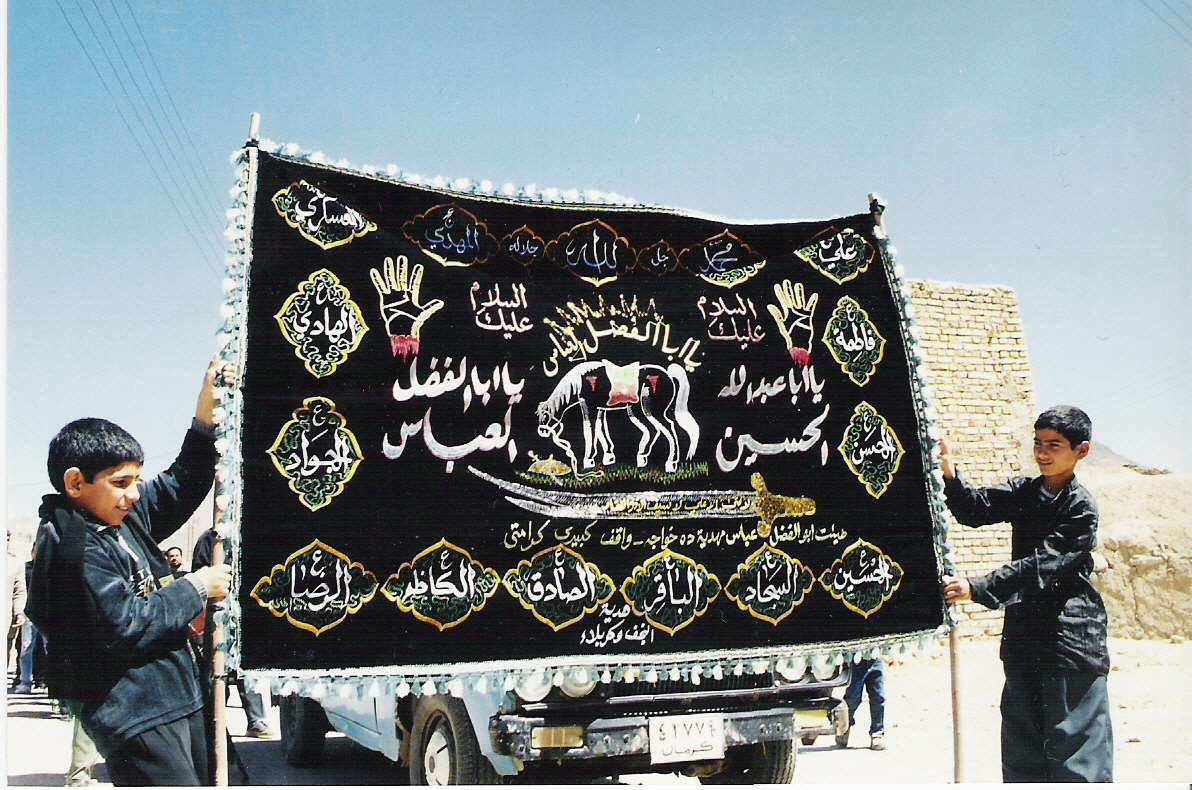
\includegraphics[width=4.07818in,height=3.13349in]{media/image6.jpeg}

\vide{les-gardiens-de-lenfer}{%
\subsubsection{3.5 Les gardiens de
l'enfer}\label{les-gardiens-de-lenfer}}

Chaque strate infernale est gardée par des anges robustes et rudes~:
«~Nous n'avons pris que des anges comme gardiens du Feu~» (S. 74, 31).
«~Des anges gigantesques et puissants se tiendront autour du Feu~; ils
ne désobéissent pas à l'ordre de dieu, ils font ce qui leur est
commandé~» (S. 66, 6). Leurs épaules sont larges. Il faut une année de
marche pour les parcourir. Ils accueillent les damnés par des flammes
aussi volumineuses que les astres. Cette tradition prend sa source
notamment dans la littérature talmudique et dans le Midrash où il est
question des anges gardant les Portes de la Géhenne.

À leur approche l'enfer gronde et mugit. Les damnés épouvantés reculent
à la vue de ces flammes, mais ils sont enchaînés par les anges. Un nuage
fait pleuvoir sur eux non l'eau qu'ils espéraient mais des chaînes. Ils
sont poussés au fond de l'enfer, mais les flammes les remontent~: S. 25,
11-13~: «~Ils ont plutôt qualifié l'Heure de mensonge. Nous avons
cependant préparé, pour quiconque qualifie l'Heure de mensonge, une
Flamme brûlante. Lorsque de loin elle les voit, ils entendront sa fureur
et ses pétillements. Et quand on les y aura jetés, dans un étroit
réduit, les mains liées derrière le cou, ils souhaiteront alors leur
destruction complète~».

\vide{description-de-lenfer}{%
\subsubsection{3.6 Description de l'enfer}\label{description-de-lenfer}}

Il y a un feu intense, mais il ne dégage aucune lumière. Un feu noir. Sa
puissance de feu est 70 fois supérieure à celui de la terre. Son
combustible est constitué des damnés dont la chair éternelle alimente
sans cesse le feu de la fournaise. Toutefois, le vendredi, le feu cesse
de brûler. Comme pour l'océan, l'enfer a un rivage. Les réprouvés y
espèrent trouver refuge et tranquillité. Mais ils s'y méprennent car ce
rivage est habité de scorpions énormes, de serpents grands comme des
chameaux. Ils les mordent et s'attaquent aux parties de leurs corps les
plus sensibles~: paupières, lèvres, organes génitaux. Leur venin est si
fort qu'il agit dans le corps 40 années durant. Finalement, ils
préfèrent encore le feu. Le chameau, la brebis ou la vache dont le
propriétaire ne s'est pas acquitté de la \emph{zakāt} sont transformés
en monstres aux cornes et aux sabots de feu qui torturent leurs
propriétaires avares et injustes. Sous les coups, leurs os sont brisés
et leurs crânes fracassés.

\vide{les-tourments-de-lenfer}{%
\subsubsection{3.7 Les tourments de
l'enfer}\label{les-tourments-de-lenfer}}

La figure des damnés sera noire, décharnée, les yeux cautérisés avec des
clous de feu, la langue allongée jusqu'au sol, le front marqué avec du
métal en fusion. Leurs lèvres seront cisaillées en deux par des ciseaux
de feu~; elles repousseront mais seront de nouveau coupées,
éternellement. Leurs bouches vomiront du pus et du sang, de la sanie qui
sera leur propre boisson. Leurs cheveux seront suspendus à des arbres de
feu, leurs entrailles brûleront, leurs dos flagellés par des chaînes de
feu. Pieds et mains enchaînés, ils devront gravir une montagne de feu.

Dans ce monde, leur corps seront plus développés pour qu'ils ressentent
plus encore la douleur. Eux aussi, ils deviennent des monstres. La chair
et la peu feront entendre une voix plus affreuse que le hurlement des
loups.

On trouve en enfer des arbres, les \emph{zaqqūm}. Les réprouvés se
nourrissent de leurs fruits, mais de feu, ils leur brûlent les
entrailles comme du métal en fusion. Plus ils en mangent, plus grande
est leur faim. Ils sont une torture. Ils boivent de l'eau bouillante et
les gardiens leur présentent une coupe débordante de pus et de sanie
bouillonnants qui proviennent de leurs corps. Leurs visages sont
décharnés, brûlés, déchirés. Tout est donc feu, souffrance, torture,
supplice. L'odeur pestilentielle des damnés les conduit à se maudire
mutuellement. C'est alors qu'ils supplient le chef des geôliers, Mālik,
d'intercéder auprès de Dieu pour atténuer leur supplice. Mais ils y
resteront à jamais, à l'exception des croyants grâce à l'intercession
des prophètes.

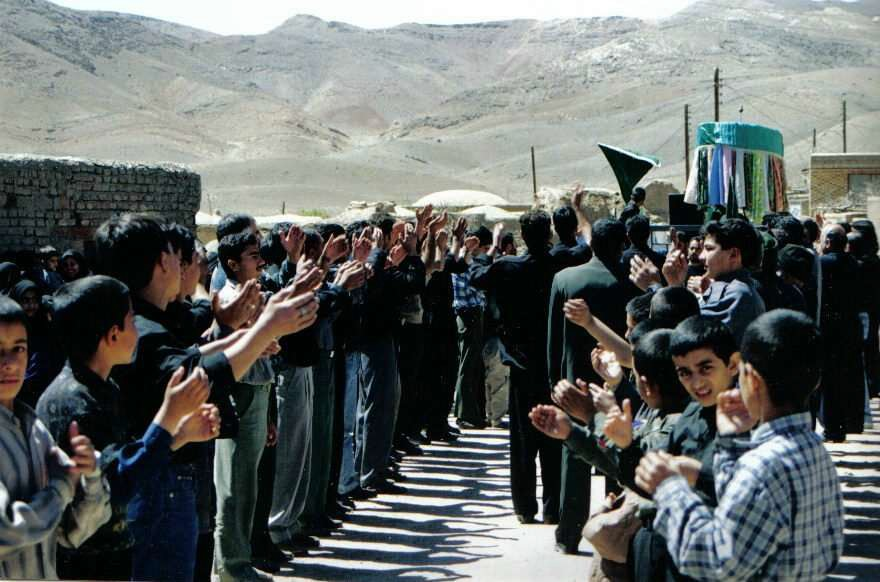
\includegraphics[width=2.73901in,height=2.05312in]{media/image7.jpeg}

\vide{la-question-de-luxe9ternituxe9-des-peines}{%
\subsubsection{3.8 La question de l'éternité des
peines}\label{la-question-de-luxe9ternituxe9-des-peines}}

Selon les exégètes traditionalistes, les souffrances sont éternelles.
Une fois plongé dans une de ces demeures, le réprouvé y reste
éternellement. Les ǧahmites qui prétendent que le paradis et l'enfer
sont des accidents et seront donc un jour anéantis sont considérés comme
des innovateurs. Toutefois, on trouve quelques traditionnistes qui
considèrent que seul le Paradis restera éternellement tandis qu'un jour,
l'enfer sera complètement anéanti.

\emph{\textbf{La position des traditionalistes}}

Ils affirment l'éternité de l'enfer et du paradis.

- Cette croyance qui s'appuie sur le consensus, \emph{iǧmā'}, des
compagnons du Prophète et de la première génération. Le consensus est
une des sources du droit musulman avec le Coran et la Sunna.

- Le Coran déclare que les tourments sont perpétuels~«~\emph{ḫalidīn
fîhā 'abadan}~», que les infidèles n'entreront pas au paradis tant que
le chameau n'entre pas dans le trou d'une aiguille~: «~Pour ceux qui
traitent de mensonges Nos enseignements et qui s'en écartent par
orgueil, les portes du ciel ne leur seront pas ouvertes, et ils
n'entreront au Paradis que quand le chameau pénètre dans le chas de
l'aiguille. Ainsi rétribuons-Nous les criminels~» (S. 7, 40). Autrement
dit, aller en enfer, c'est prendre à perpétuité.

- La tradition indique une exception à l'égard des monothéistes
(\emph{muwaḥḥid}) sujets au péché. Grâce à l'intercession des prophètes
ils peuvent sortir de l'enfer. Par suite, les infidèles sont donc quant
à eux condamnés pour toujours.

- Les anciens \emph{al-salaf}, les partisans de la tradition \emph{ahl
al-Sunna}, déclarent la création de l'enfer et du paradis avec ce
monde-ci et ils ne seront jamais anéantis. L'idée d'un anéantissement
est pour eux une innovation.

- C'est une question de justice~: le Coran distingue les fidèles des
infidèles, on ne peut mettre sur le même pied d'égalité les pieux et les
impies. La raison indique que les âmes humaines ont des qualités
immuables. Elles ne peuvent changer leurs conduites antérieures. Elles
ne peuvent donc que subir les peines éternelles.

\emph{\textbf{La critique d'Ibn Al-Qayyim al-Ǧawziyya}}

Célèbre juriste sunnite du quatorzième siècle, commentateur du Coran,
disciple d'Ibn Taymiyya, il procède à une critique de cette
interprétation.

- L'éternité de l'enfer est déjà une question disputée parmi les
compagnons. Il n'y a donc pas consensus. Pour dix des compagnons, nous
ne disposons pas de preuve quant au fait qu'ils aient nié
l'anéantissement de l'enfer. Quant à la première génération, nous
disposons clairement d'opinions controversées.

- Le Coran affirme l'éternité des tourments tant que durera l'enfer.
Tant que l'enfer existe, les infidèles y demeurent. Mais si l'enfer est
anéanti, ses membres en seront délivrés.

- Tant que l'enfer existe, en sortir est le privilège des croyants. Mais
si Dieu détruit l'enfer, les infidèles en seront donc libérés.

- Les traditions n'affirment pas l'éternité de l'enfer en soi~; elles ne
nient pas l'impossibilité de son anéantissement.

- Des compagnons ont déclaré que l'enfer sera anéanti.

- Trois passages coraniques montrent que l'enfer n'est pas éternel~: S.
6, 128~: «~Dieu leur dira: ‹l'Enfer est votre demeure, pour y rester
éternellement, sauf si Allah en décide autrement.› Vraiment ton Seigneur
est Sage et Omniscient~». S. 11, 107~: «~Pour y demeurer éternellement
tant que dureront les cieux et la terre - à moins que ton Seigneur
décide autrement - car ton Seigneur fait absolument tout ce qu'Il veut~»
ou encore~: S. 78, 23~: «~Ils y demeureront pendant des siècles
successifs~». L'éternité de l'enfer dépend donc de la volonté divine, du
Juge Suprême.

- Le Paradis exprime la Miséricorde divine, l'enfer la colère. Or, la
tradition se fait l'écho du triomphe de sa Miséricorde sur sa colère.
Les deux attributs ne sont pas égaux.

- la miséricorde est une fin tandis que la colère est un moyen. L'enfer
n'est qu'un moyen de purification. Un \emph{ḥadīṯ} rapporté par Buḫarî
indique~: «~Dieu a créé la miséricorde et en a multiplié l'aspect. Si
l'Infidèle savait tout ce que Dieu a de miséricorde, il ne désespérerait
jamais d'entrer au Paradis~»\sn{}.

- l'enfer est créé pour menacer les croyants, purifier les pécheurs. La
nature humaine est originellement pure, donc même les infidèles peuvent
être purifiés par le feu. Dieu est tel un médecin qui brûle ou coupe un
membre malade pour guérir l'homme. Il ne se plaît pas au châtiment en
soi. Ce châtiment est un aspect de sa Sagesse, de sa bonté, de sa
justice.

- certaines traditions rapportées par Ibn Hanbal indiquent que celui qui
reconnaît la bonté de Dieu, sa grâce, son pardon, alors l'Enfer devient
pour lui un séjour paisible de rafraîchissement.

- Selon un \emph{hadiṯ qudsi}, la miséricorde de dieu embrasse toutes
choses~: 
\begin{quote}
    «~Je ne fais pas perdre à ceux qui me désobéissent l'espoir de
ma Miséricorde. S'ils reviennent de leur erreur, je suis leur
bien-aimé~; et s'ils ne reviennent pas je suis leur médecin. Je leur
fais subir les peines pour les purifier de leurs erreurs~!~»
\end{quote}


\vide{le-paradis-selon-lislam}{%
\subsection{Le paradis selon l'islam}\label{le-paradis-selon-lislam}}

\vide{existence-localisation-et-duxe9signation}{%
\subsubsection{Existence, localisation et
désignation}\label{existence-localisation-et-duxe9signation}}

L'existence du Paradis est affirmée dans le Coran. Selon l'exégèse
traditionnelle, il existe dès à présent, dans un septième ciel. Il a été
créé par Dieu en même temps que notre monde ici-bas comme lieu de
récompense pour les bienheureux (S. 3, 133).

Il existe dans le Coran plusieurs termes pour désigner le paradis.

Le vocable le plus courant est celui de \emph{Ǧanna}, le Jardin. Le
Coran en précise sa nature en évoquant «~le Jardin de la retraite~»
(\emph{Ǧannat al-Ma'wā}, S. 53, 15), le «~Jardin des délices~»
(\emph{Ǧannat an-Na`īm}, S. 10, 9). Il est aussi question du Jardin
d'Eden (\emph{Ǧannat} \emph{`Adn}, S. 61, 12), jardin de bonheur.

Quatre autres expressions sont utilisées pour désigner le paradis~:
\emph{Dâr al-Salām}, la demeure~du salut (S. 6, 127) ; \emph{Dār
al-Muqāma}, la demeure illimitée (S. 35, 35)~; \emph{Dār al-ḫuld}, la
demeure de l'éternité (S. 25, 15) ou encore \emph{dār}
\emph{al-ḥayawān}, la demeure de la vie éternelle (S. 29, 64). On trouve
une autre expression, Firdaws (S. 23, 11) qui est un dérivé du
\emph{Pardes} persan.

\vide{description-du-paradis}{%
\subsubsection{Description du
paradis}\label{description-du-paradis}}

Les descriptions du Paradis sont nombreuses et la littérature
\emph{ḥadīṯ} en donne des images empruntes d'une grande sensualité et
beauté. Il est question d'un lieu de palais aux voutes de perles, de
tapis de fleurs, d'arbres aux couleurs jusqu'alors inconnues des hommes,
les jujubiers d'al-\emph{Muntahā}.
\begin{quote}
    S. 4, 57~: «~Et quant à ceux qui ont cru et fait de bonnes œuvres,
bientôt Nous les ferons entrer aux Jardins sous lesquels coulent des
ruisseaux. Ils y demeureront éternellement. Il y aura là pour eux des
épouses purifiées. Et Nous les ferons entrer sous un ombrage épais».
\end{quote}


On y trouve des fleuves comme dans le paradis terrestre de la Genèse,
mais il n'y coule pas seulement de l'eau~:
\begin{quote}
    «~Il y aura là des fleuves dont l'eau est incorruptible, des fleuves de
lait au goût inaltérable, des fleuves de vin, délices pour ceux qui en
boivent, des fleuves de miel purifié. Ils y trouveront aussi toutes
sortes de fruits et le pardon de leur Seigneur (S. 47, 15)~».
\end{quote}


Cette description rappelle la description de la Terre promise aux
Hébreux dans l'Ancien Testament. Elle était désignée comme une terre où
ruissellent le lait et le miel (Ex 3, 8, 17 ou Ex 13, 5~; Deut 6, 3,
etc.). C'est un pays d'abondance, de source d'eau, de vigne\ldots Le
2\textsuperscript{ème} Livre d'Hénoch et l'Apocalypse de Paul évoquent
aussi les ruisseaux de miel, de lait, de vin et d'huile.

Il y a des vierges éternelles~:
\begin{quote}
    «~ Là, il y aura des vertueuses et des belles.\\
Lequel donc des bienfaits de votre Seigneur nierez-vous~?\\
Des houris cloîtrées dans les tentes,\\
Lequel donc des bienfaits de votre Seigneur nierez-vous~?\\
qu'avant eux aucun homme ou djins n'a déflorées.\\
Lequel donc des bienfaits de votre Seigneur nierez-vous~?\\
Ils seront accoudés sur des coussins verts et des tapis épais et
jolis.\\
Lequel donc des bienfaits de votre Seigneur nierez-vous~? (S. 55,
70-77)~».
\end{quote}


Et des éphèbes : 
\begin{quote}
    «~ Parmi eux circuleront des garçons éternellement
jeunes,\\
avec des coupes, des aiguières et un verre (rempli) d'une liqueur de
source\\
qui ne leur provoquera ni maux de tête ni étourdissement;\\
et des fruits de leur choix,\\
et toute chair d'oiseau qu'ils désireront.\\
Et ils auront des houris aux yeux, grands et beaux,\\
pareilles à des perles en coquille\\
en récompense pour ce qu'ils faisaient (S. 56, 17-24) ».
\end{quote}

On peut y boire du vin car il n'enivre pas~:
\begin{quote}
   «~On leur sert à boire un nectar pur, cacheté, laissant un arrière-goût
de musc.

Que ceux qui la convoitent entrent en compétition (pour l'acquérir)\\
Il est mélangé à la boisson de Tasnīm,\\
source dont les rapprochés boivent (S. 83, 25-28)~». 
\end{quote}


Ce qui est à relever dans ces descriptions, c'est l'atmosphère de
banquet qui y règne. Les élus sont accoudés sur des tapis aux revers de
brocart\ldots{} sur des coussins verts et sur de beaux tapis (S. 55, 54
et 76), ils boivent un vin délectable. Ces images sont typiques de la
tradition juive qui sert à décrire le bonheur des justes.

\vide{accuxe8s-au-paradis}{%
\subsubsection{Accès au paradis}\label{accuxe8s-au-paradis}}

Le Paradis est constitué de différents étages. La tradition distingue
huit portes qui ouvrent à différents espaces paradisiaques et qui
s'ouvrent en fonction des actions accomplies par les croyants. Il y a
ainsi la porte de la prière, de la guerre sainte, de l'aumône, du jeûne,
du repentir, des patients (ceux qui maîtrisent leur colère), de la
soumission à la volonté divine, enfin la porte droite celle qui ne
nécessite pas de jugement préalable~: c'est elle qu'emprunte Muḥammad.

Il est nécessaire pour entrer au paradis d'avoir un laisser passer et
selon une tradition, chaque croyant entrera au paradis avec un passeport
sur lequel sera indiqué~: 
\begin{quote}
    «~Au nom de Dieu, le Bienfaiteur, le
Miséricordieux. Nous délivrons à \ldots{} fils de\ldots{} un permis
d'entrée au jardin sublime, dont les fruits à cueillir seront à portée
de sa main~».
\end{quote}

Les élus sont accueillis par un chœur d'anges qui chante en arabe, ils
ont un visage radieux après avoir été lavés dans une douce fontaine.

Le climat du Paradis est doux~: «~Il n'y sévit ni la chaleur du soleil,
ni la rigueur du froid (S. 75, 3). Les mois comprennent 500
jours\ldots{} et les années 500 mois.

\vide{les-uxe9lus}{%
\subsubsection{Les élus
}\label{les-uxe9lus}}

Ils ont l'apparence d'un homme âgé de 33 ans, ils sont imberbes.

Toute épouse vierge au moment du mariage sera la femme légitime du
Bienheureux au paradis. Le Bienheureux qui a eu plusieurs épouses les
gardera toutes. Si la femme a eu plusieurs maris, elle se consacrera au
dernier, au meilleur ou à celui de son choix.

\vide{la-question-des-femmes-au-paradis}{%
\subsubsection{La question des femmes au
paradis}\label{la-question-des-femmes-au-paradis}}

Mais justement, revenons sur la question de la femme.

Le Coran est explicite quant à l'égale possibilité pour les hommes et
les femmes d'accéder au paradis ou en enfer~:
\begin{quote}
    «~Et quiconque, homme ou femme, fait de bonnes oeuvres, tout en étant
croyant... les voilà ceux qui entreront au Paradis; et on ne leur fera
aucune injustice, fût-ce d'un creux de noyau de datte~» (S. 4, 124).



«~{[}Il en est ainsi{]} afin qu'Allah châtie les hypocrites, hommes et
femmes, et les associateurs et les associatrices, et Allah accueille le
repentir des croyants et des croyantes. Allah est Pardonneur et
Miséricordieux~» (S. 33, 73).
\end{quote}
Il semble cependant qu'il y ait en enfer plus de femmes que d'hommes.
Ceci est indiqué dans un \emph{ḥadīṯ} alors que Muḥammad eut une
vision~: 
\begin{quote}
    «~J'ai vu le feu et je n'ai pas vu à ce jour un spectacle plus
terrible. La plupart des habitants sont des femmes~». la raison en est
leur ingratitude, leur manque de charité, leur négativité dans le regard
des actions conduites par leurs maris~: «~si les hommes font de bonnes
choses, la femme voit une chose mauvais, et vous dit qu'elle n'a jamais
rien vu de bon du tout~» (Ahmad ibn Hanbal, I.359, cité dans Smith et
Haddad 1975: 44).
\end{quote}


Le Coran mentionne les femmes de Lot et de Noé qui à cause de leur
trahison furent conduites au Feu. Leurs saints maris ne leur furent
d'aucun secours~: 
\begin{quote}
    «~Allah a cité en parabole pour ceux qui ont mécru la
femme de Noé et la femme de Lot. Elles étaient sous l'autorité de deux
vertueux de Nos serviteurs. Toutes deux les trahirent et ils ne furent
d'aucune aide pour {[}ces deux femmes{]} vis-à-vis d'Allah. Et il
{[}leur{]} fut dit: ‹Entrez au Feu toutes les deux, avec ceux qui y
entrent~» (S. 66, 10).
\end{quote}


Notons que parmi les signes de la venue du jugement dernier, on trouve
mentionné le renversement des valeurs morales traditionnelles entre
l'homme et la femme~: l'homme doit obéir à sa femme et il désobéit à ses
parents, l'homme doit travailler pour sa femme, les femmes vont au
pèlerinage ensemble sans être accompagnées d'un homme, il y a une pleine
licence sexuelle. Le nombre d'homme décroît tandis qu'il y a cinquante
femmes pour un homme.

\vide{la-question-des-houris}{%
\subsubsection{La question des
houris}\label{la-question-des-houris}}

Houris vient du mot arabe \emph{ḥawrâ'}, pluriel de \emph{ḥur.}

\emph{Le Coran} mentionne à plusieurs reprises les houris~:
\begin{quote}
   S. 44, 54~: «~C'est ainsi! Et Nous leur donnerons pour épouses des
houris aux grands yeux~». 
S. 55, 56~: «~Ils y trouveront {[}les houris{]} aux regards chastes,
qu'avant eux aucun homme ou djinn n'aura déflorées~».

S. 52, 20~: «~accoudés sur des lits bien rangés›, et Nous leur ferons
épouser des houris aux grands yeux noirs~».

S. 55, 72~: «~des houris cloîtrées dans les tentes~».

S. 56, 22~: «~Et ils auront des houris aux yeux, grands et beaux~»
\end{quote}




Quant au ḥadīṯ, on trouve dans la compilation de al-Buḫarî~\sn{Livre 54, \emph{Le commencement de la création}, ḥadīṯ 476.}:
\begin{quote}
    Le Prophète a dit: «Les premières personnes qui entreront au paradis
seront brillantes comme la pleine lune, et les suivantes brillantes
comme l'étoile la plus brillante dans le ciel. Leurs cœurs seront comme
le cœur d'un seul homme, car ils n'auront ni haine ni jalousie entre
eux, tout le monde aura deux épouses, des houris, qui seront aussi
belles, pures et transparentes que la moelle des os de leurs jambes~»

\end{quote}


Autre hadîth de Buḫari~: rapporté par Abu Huraira: 
\begin{quote}
    «~L'Apôtre d'Allah
dit: «Les premières personnes à entre au paradis, seront brillantes
comme la pleine lune et celles qui les suivront, brilleront comme
l'étoile la plus brillante dans le ciel. Ils n'urineront pas, ils ne se
soulageront pas, ils ne cracheront pas et n'auront pas de sécrétions
nasales. Leurs peignes seront d'or, et leur sueur d'une odeur de musc.
Leurs épouses seront des houris. Elles ressembleront toutes à leur père
Adam (dans leur état), elles seront grandes de soixante coudées de
hauteur~».
\end{quote}


\paragraph{Les commentateurs}

Elles ont suscité plusieurs questions

\begin{itemize}
\item
  sont-elles de la même essence que les femmes~?
\item
  sont-elles de la lignée d'Eve~?
\item
\end{itemize}

Pour certains commentateurs, elles ont été créées de safran. Mais elles
semblent bien être faites de chair. Leur luminosité y est dépeinte dans
un style hyperbolique~: leurs sourcils ressemblent à un trait noir placé
sur de la lumière et leur front rappel un croissant de lune.

Les commentateurs se sont aussi interrogés sur les délices qu'elles
peuvent procurer aux croyants~? Combien de houris un Croyant peut-il
honorer de ses faveurs par nuit~? Des réponses diverses qui montrent
cependant que l'occupation principale au paradis sera de s'enlacer de ces
femmes vierges. Et le plaisir de l'homme y sera décuplé de 100 fois de
celui sur terre. Elles attendent au ciel leurs époux et maudissent leurs
femmes terrestres lorsque celles-ci se fâchent ou les contrarient leurs
maris.

Les houris sont pures. Elles ne souffrent des aléas de la menstruation,
elles n'éprouvent aucune fatigue. Les élus mangent les fruits délicieux
du paradis par pure jouissance. Les résidus de la digestion se
transforment en une exhalation parfumée du corps.

\paragraph{L'hypothèse syriaque}

En l'an 2000, un chercheur libanais-allemand sous le pseudonyme de
Christoph Luxenberg a publié un ouvrage intitulé \emph{Die
Syro-Aramäische Lesart des Koran:~ Ein Beitrag zur Entschlüsselung der
Koransprache} \sn{en français~: \emph{Lecture syro-araméenne du Coran~: une
contribution pour décoder la langue du Coran}}. Cet ouvrage est une
étude philologique qui met en lumière l'existence particulière d'une
source du Coran. Si nombreux sont les auteurs qui ont souligné
l'influence des textes bibliques, Luxenberg indique l'adoption plus
particulière d'un lectionnaire syriaque, et plus particulièrement d'un
ouvrage liturgique à vocation ce missionnaire. Ces travaux poursuivent
l'enquête menée par Günther Lulling.

Sa méthodologie consiste à rechercher les équivalents syriaques des
termes arabes et de clarifier le sens de certains passages coraniques
obscurs à l'aide des termes syriaques.

À cet égard, le mot houri signifierait non pas une vierge aux grands
yeux noirs, mais du raisin blanc.

\vide{conclusion-la-vision-de-dieu}{%
\section{{Conclusion~: La vision de Dieu
}}\label{conclusion-la-vision-de-dieu}}

La question de la vision de Dieu n'est pas étrangère à la tradition
musulmane. Elle y est affirmée parfois de manière explicite~: Chaque
vendredi, hommes et femmes rendent visite au Seigneur sur son
invitation. Chemin faisant, ils passent devant le tableau du Destin,
\emph{al-Lawḥ al-mahfūẓ} où se trouvent consignées toutes les actions
des êtres. Sur des montures ailées, les Bienheureux parviennent en un
clin d'œil devant le Trône du Tout-Puissant. Le voile de lumière se lève
et l'Eternel paraît. La voix divine retentit~: «~al-salām alaykum~». La
vue de Dieu surpasse tous les délices du paradis.

Si l'ensemble de ces descriptions sont marquées par une très grande
sensibilité, il ne faut pas oublier, à l'exemple du cours sur la
philosophie, qu'elles ont donné lieu à des interprétations et à une
lecture spirituelle. Ainsi, al-Ġazālī soutient que la vision de Dieu
relève de l'ordre de la connaissance~: voir Dieu, c'est accéder non à
une vision physique, mais à sa connaissance.



\chapter{L'Islam comme religion Universelle ?}


L'Islam semble offrir aujourd'hui deux visages au voyageur candide qui
observe le monde. D'un côté, il peut admirer des mosquées magnifiques en
forme de pagodes, avec des stèles traditionnelles chinoise, à Xi'an,
ancienne capital de la Chine~; de même la Mesquita à Cordoue, l'art
Moghol en Inde, qui s'inspire des influences architecturales locales
tout en créant un univers inédit et reconnaissable. Et au-delà de
l'architecture, il peut rencontrer des musulmans de toutes les Nations.
De l'autre, il peut observer régulièrement une sorte de séparation par
des pratiques ou des tenues, qu'il retrouve à travers le monde, tunique,
barbe, et chaussure Nike, sans parler de la tenue des femmes et du
fameux \emph{voile}.

Au deuxième siècle de notre ère, chrétiens et juifs répondirent de façon
très différente, à la question du rapport au monde, le rabbin Tryphon
faisant la remarque aux chrétiens que \sn{Dialogue de saint Justin
  avec le juif Tryphon. Chapitre 10.«~Mais ce qui nous embarrasse surtout, c'est que vous vous dites
  pieux; que vous estimez différer des autres tout en ne vous en
  séparant pas; et que dans votre vie, vous n'êtes pas différents des
  nations, puisque vous n'observez ni les fêtes, ni les sabbats, que
  vous n'avez pas la circoncision; et encore, tandis que vous mettez
  votre espoir en un homme qui a été crucifié, vous espérez en même
  temps quelque bien de Dieu, sans observer ses commandements.}
  \begin{quote}
       «~vous
vous dites pieux; vous estimez différer des autres tout en ne vous en
séparant pas; et dans votre vie, vous n'êtes pas différents des nations,
puisque vous n'observez ni les fêtes, ni les sabbats, que vous n'avez
pas la circoncision~».
  \end{quote}



Qu'en est-il de l'Islam~? Quel est son rapport à l'universalité~?
Question qui nous semble être un préalable à d'autres questions, comme
celle de la possibilité d'un \emph{Islam de France} ou de son rapport à
la démocratie\emph{.} Nous proposons d'étudier la réponse faite en 1882
par Abraham Kuenen. Cette année-là, ce théologien hollandais de
l'université de Leyde, spécialiste reconnu du Pentateuque, et l'un des
pères de l'approche \emph{historico-critique.} se rend en Angleterre
pour dispenser un cours, intitulé \emph{National Religions et Universal
Religion}. Il s'attache alors, avec rigueur à tester ces deux concepts
de religion nationale et religion universelle à l'Islam~: \emph{l'Islam
offre-t-il les caractères de l'universalisme religieux}~? \sn{Kuenen,
  A. ``\emph{L'Islam offre-t-il les caractères de l'universalisme
  religieux}?'' Revue De L'histoire Des Religions, vol. 6, 1882, pp.
  1--40. JSTOR,
  \url{http://www.jstor.org/stable/23658819}.}
Les 150 ans qui nous sépare de cette conférence, bien loin de constituer
un handicap, permettent de se situer à une période précédent la fin de
l'empire Ottoman - et de son paradigme \emph{l'Islam Impérial ou
classique}\sn{Adrien Candiard, \emph{Comprendre l'islam: ou plutôt
  : pourquoi on n'y comprend rien, 2016,} emp. 427}\emph{,} en nous
offrant un recul utile pour répondre à cette question de
l'universalité\emph{.} Nous proposons dans un premier temps d'étudier
les différentes étapes du raisonnement de Kuenen qui l'amène à ne pas
attribuer le terme de \emph{religion universelle} à l'Islam puis dans un
second temps, de proposer quelques éléments qui nous semble permettre
d'atténuer ce jugement en particulier en testant les présupposés
méthodologiques de Kuenen et en proposant quelques pistes entrevues lors
du cours sur les fondations de l'Islam.

\section{La thèse de Kuenen : L'islam comme religion particulière}
Pour répondre à la question posée par l'Islam, il nous faut d'abord
définir ce qui définit une religion universelle par rapport à une
religion nationale, bornée à un peuple unique ou à une groupe de peuples
de mêmes origines. Kuenen propose de ne pas s'arrêter au fait (l'Islam a
bien été adopté par plusieurs nations différentes et est une religion
internationale), mais de regarder son caractère propre. \sn{car
  «~le universel de fait peut venir de la force au moins en dépit de son
  caractère propre~; que son défaut ou du moins sa faiblesse en fait
  d'éléments vraiment universels ait trouvé sa contrepartie ou son
  dédommagement dans différentes particularités qui ne viennent pas en
  ligne de compte quand on dresse son signalement\emph{~».}} Mais
comment définir le caractère propre d'une religion~? Fidèle à sa méthode
historico-critique\sn{Kuenen a établi quatre règles permettant
  l'interprétation d'un texte~:

  \emph{rigueur philologique et grammaticale}, c'est-à-dire conditionnée
  par le contexte de l'époque et le style de l'auteur.

  \emph{rationnellement cohérente}, un passage doit toujours être
  interprété dans son contexte

  \emph{historique}, c'est-à-dire en correspondance avec les données
  historiques à notre disposition

  \emph{psychologique}, elle doit nous rendre l'état mental préalable au
  texte.} permettant de remonter à l'origine du texte, il essaye de
ressaisir «~l'élément authentiquement universel {[}\ldots{]} qui tient
immédiatement à l'origine~»\sn{Ibid, p. 5 «~élément
  authentiquement universel, n'est pas à mon sens, l'effet d'une
  addition postérieure, mais tient immédiatement à l'origine des
  religions dans lesquelles nous saisissons cet élément, à la nature du
  rapport ou elles se trouvent avec les religions nationales d'où elles
  sont sorties ou sur le terrain desquelles elles se sont développées.~»}
de l'Islam. Nous connaissons relativement bien cette origine, d'une
religion née «~en pleine lumière~» selon l'expression de Renan. Pour
bien capter cette origine, Kuenen étudie les religions nationales qui
précèdent, et en particulier la \emph{Hanîffyya,} la religion d'Abraham
telle qu'elle est mentionnée dans la Sira (I, 222-232)\sn{Ce
  passage de la Sira mentionne 4 \emph{hanifs}, qui anticipent la venue
  de Mohammed. «~Zayd ibn 'Amr ibn Nufayl~{[}\ldots{]} interrogea le
  moine sur la \emph{Hanîfiyya}, la religion d'Abraham. «~Tu recherches
  une religion à laquelle tu ne trouveras personne aujourd'hui pour te
  conduire. Cependant, le temps est proche où un prophète sortira de ton
  pays que tu viens de quitter et prêchera la religion d'Abraham.
  Rejoins-le, car c'est bien la période prévue pour sa mission.~Hichâm,
  Ibn. \emph{La biographie du prophète Mahomet}, Sira I, 222-232}. Mais
il conclut que nous ne savons pas grand-chose de ces \emph{hanifs} et
que la référence à Abraham est probablement un \emph{hysteron proteron,}
une reconstruction ex-post permettant de faire le lien avec les juifs et
chrétiens mais sans se lier à eux\sn{Cf «~Abraham ne fut ni juif
  ni chrétien, mais fut \emph{hanif} et \emph{muslim} {[}à Allah{]}. Et
  il n'était point du nombre des Associateurs » (Coran 3:67)}.

Le contexte n'explique donc par l'Islam et c'est donc vers Mohammed
qu'il faut se tourner~: «~l'islam est bien plus que la plupart des
autres religions, le produit non d'une époque, non d'un peuple, mais de
la personne de son fondateur~»\sn{Ibid, p. 17}. Kuenen le décrit
comme un homme religieux, surtout avant la fuite à Médine, avec une
\emph{pensée sémitique,} en particulier par son eschatologie marquée par
le judaïsme.

L'Islam valorise dès son origine le Coran, glorifié à l'intérieur même
du Coran. Il transmet certes un noyau du Judaïsme transporté sur le sol
d'Arabie. Mais Mohammed avait une vision plus large, comme le soulignent
différentes sourates.~: «~le Coran, est en vérité un avertissement pour
toutes les créatures~»\sn{Ref Coran 8,87~?}, «~nous ne t'avons pas
envoyé aux hommes en général que pour prêcher et menacer, cependant la
plupart des hommes ne comprennent pas~»\sn{Coran 34,27}.~

Mais Kuenen constate en parallèle de ces versets, de nombreux passages
qui valorise les Arabes, ce qui semble limiter cette vocation à
l'universel\sn{« avec quelle extrême insistance est relevé le
  privilège des Arabes qui, dans les signes qui leur ont été montrés,
  c'est-à-dire dans les versets du Qurân, possèdent maintenant la parole
  même d'Allah, {[}qui dépasse{]} de beaucoup (celles qu'ont reçue les
  fondateurs des autres religions) » Ibid, p.18}. De plus, il souligne
des exceptions à l'universalité, qui semblent même s'opposer
formellement à l'essence de l'Islam, comme la Ka'ba et la mise en
exergue de la Mecque, «fragment incompréhensible de paganisme qui est
passé dans l'islam sans être digéré~»\sn{Ibid, p 24}.

Mais alors comment comprendre que l'Islam soit devenu \emph{de fait} une
religion universelle. Pour Kuenen, cela vient de la pauvreté de
l'essence de l'Islam, de sa plasticité dirions-nous aujourd'hui, qui lui
permet de dériver des variétés persane, hindoue ou javanaise. La
simplicité et la concision d'une religion sont pour Kuenen le plus grand
éloge qu'on puisse lui faire à la condition qu'elle permette le
développement spirituel de l'homme, ou qu'au moins elle n'y fasse pas
obstacle. «~A cette condition, mais à cette seule condition, elle peut,
en dépit de son étroitesse, avoir un caractère universel, être une
bénédiction pour l'humanité. »\sn{Ibid, p 26}. Ce n'est pas au
niveau de la vie politique ou juridique qu'est l'enjeu mais bien dans
«~la vie de l'âme et de la conviction religieuse~». Mais Kuenen
considère que de cette pauvreté spirituelle originelle vient de la foi
même de l'Islam~: Allah est certes~\emph{ar-rahmano'r-rahimo,~} le
miséricordieux et le compatissant mais il est surtout «~un dieu de
loin~»\sn{Ibid, p 32} dont il faut suivre les devoirs religieux
prescrits par lui. Pour compenser cet éloignement, les croyants ont
développé par la suite des éléments mystiques, comme le soufisme et la
foi en la \emph{médiation}, soit de Mohamed, soit des saints (dont le
culte est fervent dans l'Islam du XIX\textsuperscript{ème} siècle). Mais
pour le culte des saints, il remarque qu'il est «~plutôt une
protestation contre la religion~»\sn{Ibid, p 31}~: le musulman
recherche ce que sa foi ne lui fournit pas et il le cherche là où,
d'après l'autorité même qu'il reconnait, il ne devrait pas le chercher.
De même pour le soufisme~: le vrai soufi vit une vie intérieure
remarquable mais n'est plus musulman\sn{Ibid, p 31}.

Mais alors qu'est-ce que l'Islam~? Mais «~malheureusement, la foule
n'avait pas tort~» quand elle s'opposait aux rationalistes Mo'tazilites.
En imposant le Coran incréé, la foule a «~barré à leur religion la voie
qui conduit au véritable universalisme. Car l'élément éthique est
l'élément universellement humain~».\sn{Ibid, p 36}

\subsection{Le Wahhabisme comme véritable Islam}
Pour Kuenen, le wahhabisme est le \emph{véritable islam}\sn{Ibid,
  p 37}, formule étonnante quand on pense qu'elle a été écrite il y a
150 ans. Cette doctrine enseignée par Mohammed ben Abdelwahhab en
XVIIIème siècle, propose une forme intransigeante de l'Islam, s'opposant
à tout ce qui ressemble à de l'associationisme, luttant en particulier
contre le culte des saints ou des soufis et prêchant une application
stricte de la loi~: il commande ainsi l'exécution publique par
lapidation d'une femme adultère. En 1880, le wahhabisme est aux franges
géographiques et théologiques du sunnisme, considéré comme hérétique par
l'\emph{Islam Impérial} et réduit aux habitants de l'oasis du
\emph{Nejd,} au centre de l'Arabie. Même si Kuenen n'est pas sûr de son
succès, il reconnaît dans le wahhabisme, la cohérence avec le message et
la pureté originels de l'Islam\sn{Ibid, p 37}. Ses
caractéristiques «~ témoignent d'une façon aussi décisive contre
l'universalisme de l'Islam. Une religion qui peut ainsi être restaurée
en retournant à bon escient à ses origines authentiques, peut répondre
aux besoins des habitants du désert qui l'a vue naître, elle est
incapable de satisfaire des besoins différents et plus
élevés~»\sn{Ibid, p. 38}.

Finalement, l'Islam est une religion nationale, «~un gourmand du
Christianisme, et plutôt encore, disons-nous, du judaïsme~: un extrait,
pour ainsi dire, de la Loi et de l'Evangile fait par un Arabe et pour
les Arabes, calculé d'après leurs capacités et {[}\ldots{]} gâté
devrions-nous dire par des éléments nationaux qui devaient rendre
l'acceptation facile~».\sn{Ibid, p. 39}
\section{Limites de la thèse de Kuenen}
On ne peut réfuter facilement la conclusion de Kuenen, de par la rigueur
de sa démonstration présentée ici rapidement, sa connaissance de
l'Islam, et certaines conclusions qui apparaissent comme prescientes,
comme l'importance théologique du wahhabisme bien avant son
développement numérique. Il nous semble néanmoins que l'avocat de la
défense peut avancer quelques éléments.

Le premier élément, concerne le cadre épistémologique c'est à dire la
\emph{méthode} de Kuenen de chercher à définir le religion telle qu'elle
était \emph{à l'origine}. De nombreux théologiens suivaient la même
approche au XIXème~: ainsi, Adolf Harnack essayait de retrouver le
christianisme originel, que n'aurait pas corrompu l'Hellénisme des
premiers siècles de notre ère. Or, nous savons depuis Albert
Schweitzer\sn{Dans son \emph{Histoire des recherches sur la vie de
  Jésus} (1906) il met en évidence la grande diversité des
  interprétations de Jésus, toutes anachroniques. Il nous faut accepter
  cette distance irréductible, marquée aussi par l'existence de 4
  Evangiles et non d'un seul.} que ce retour à l'origine nous est
impossible~: ce que nous trouvons dans ce passé est largement ce que
nous y projetons, d'où le caractère anachronique et daté de ces
reconstructions des origines. D'une certaine façon, c'est la limite de
l'écriture seule, \emph{scriptura sola}, qui réfute toute légitimité à
la tradition. Or, toute écriture, pour être vivante, a besoin d'un corps
de croyants, qui \emph{confesse} sa foi et transmet le message originel
en l'adaptant à la culture et la langue actuelle\sn{Et comme
  inversement chaque tradition a besoin de se laisser convertir par
  l'Ecriture pour rester authentique}.

Ainsi, par méthode, il est normal que Kuenen identifie le wahhabisme
comme le véritable Islam, avec son projet théologique de retour aux
sources. Mais est-ce le véritable Islam~?

Imiter les \emph{salaf}, les pieux anciens des trois premières
générations musulmanes, encore préservé de la dégradation progressive de
la tradition\sn{Comprendre les crises de l'islam contemporain
  \textgreater{} Emplacement 500}, est-ce l'islam ou bien une projection
des attentes et des frustrations des musulmans des lieux et époques où
wahhabisme et salafisme sont nés\sn{A ce titre, il n'est pas
  anodin que le wahhabisme apparaisse justement au XVIIIème siècle quand
  la décadence de l'Empire Ottoman apparait évident, sous le règne du
  calife Moustafa III~ et le pouvoir des janissaires.}. Seuls les
musulmans d'aujourd'hui peuvent dire ce qu'est le véritable Islam.

Et à ce titre, la critique de Kuenen du wahhabisme est particulièrement
pertinente et mérite d'être entendu~: si les musulmans dans leur
ensemble décidaient que le véritable Islam, c'est le wahhabisme (ou le
salafisme), n'y a-t-il pas un véritable risque de fermeture à
l'universel~? La théologie de l'école hanbalite\sn{Adrien
  Candiard, \emph{Du fanatisme,} 2020, le Cerf. Emplacement 153} met au
centre de son approche l'absolue transcendance de Dieu car « Rien n'est
semblable à Lui » \sn{Coran 42 , 11}. Nous ne pouvons connaître
que ce qu'Il nous fait connaître à travers le Coran. Mais ce qu'il a
révélé d'après la théologie hanbalite, ce n'est pas sa nature,
inaccessible pour l'homme, c'est sa \emph{volonté}. On a pu qualifier
cette théologie de «pieux agnosticisme », c'est-à-dire une théologie qui
pense sa propre inutilité. Seul compte notre action, celle de faire Sa
volonté, et non point notre for intérieur. Adrien Candiard prend
l'exemple d'une fatwa de Ibn Taymiyya. Ce grand théologien rigoriste de
l'école hanbalite est aujourd'hui très influent auprès des milieux
salafistes. Il répond dans cette fatwa à ce qu'il convient de penser des
musulmans qui participent, avec les chrétiens, aux réjouissances qui
entourent le jour de Pâques. Si être musulman, c'est faire ce que Dieu a
commandé (prières,\ldots), de manière symétrique, se réjouir de Pâques,
c'est «~être chrétien~», et donc coupable d'apostat. D'où l'engouement
de l'islam contemporain pour des questions jusque-là marginales, ,
qu'elles soient alimentaires ou vestimentaires~: le voile, manger des
pastèques\ldots{} «~avoir la foi, c'est inscrire dans sa chair même sa
soumission à la loi divine , en portant la barbe ou le voile, en
affirmant visiblement cet amour de la loi. Reprocher à ces croyants de
se perdre dans des détails secondaires et d'en oublier l'essentiel, la
relation à Dieu, c'est entamer un parfait dialogue de sourds
.~»\sn{Candiard, Ibid, Emplacement 206} Le wahhabisme peut
présenter un réel pouvoir d'attraction en dehors du monde arabe du fait
de son caractère très normé, cohérent et peut être même par l'absence de
for intérieur dans un monde changeant et complexe. Est-ce que cela peut
nourrir le besoin spirituel de l'homme~? Nous aimerions, avec Kuenen,
pouvoir répondre par la négative, tant l'image de l'homme qu'elle
véhicule est pessimiste, si éloignée de celle d'un homme \emph{pneumo
spermatikon,} ouvert à la raison et à l'esprit de Dieu.

Kuenen propose l'éthique comme le seul élément universellement humain.
Même si le véritable Islam ne peut se réduire au seul wahhabisme, est-ce
que l'Islam est ouvert à la réflexion éthique, malgré la condamnation de
l'école muza'lite ou bien la pense-t-il dans la limite des devoirs
religieux prescrits par Dieu ? Il faut tout d'abord rappeler
l'importance dans le Coran des limites à mettre à la raison de l'homme
(\emph{Voilà les limites d'Allah. Ne les transgressez donc pas. Et ceux
qui transgressent les ordres d'Allah ceux-là sont les
injustes}.\sn{S.2, 229}). Mais la compréhension de ces limites est
sujet à plusieurs écoles juridiques, hanbalite, mais aussi hanafite,
malikite et le šafi`ite, qui font jouer différemment Coran, hadiths,
coutume et raison ~: il y a donc déjà au sein même de l'Islam une vraie
diversité d'interprétation de la \emph{volonté de Dieu} à suivre,
diversité qui en elle-même permet de dessiner un premier niveau
d'éthique.

Mais plus fondamentalement, au-delà de ces écoles, l'enjeu éthique
concerne aussi la place des devoirs religieux\emph{.} Faut-il tout
formaliser, tout codifier dans la vie du croyant~ou bien plutôt penser
la \emph{šarī`a,} terme qui n'apparaît qu'une fois dans le Coran non pas
une Loi mais une méthode, une voie\sn{Selon le réformateur Rašīd
  Riḍā (m. 1935) \emph{Le Califat}, cité dans le cours.}. Et de même,
penser le \emph{fiqh}, cette formalisation de la loi divine en
prescriptions pratiques, plutôt comme un éveil à la vie spirituelle, en
s'inspirant du grand penseur musulman 'Al-Ġazālī  \sn{« la science de la voie qui mène à la vie de
  l'Au-delà, la connaissance détaillée des maladies de l'âme, de ce qui
  rend les œuvres corrompues, de la puissance avilissante de ce
  bas-monde, de la force d'aspiration des délices du Paradis et de
  l'emprise de la peur sur le cœur » Al-Ġazālī, \emph{Le livre de la
  science}, Paris, La Ruche, p. 58-59.}

\begin{quote}
    

«~C'est le \emph{fiqh} entendu en ce sens qui éveille et avertit et non
les définitions de la répudiation (\emph{talāq}), de l'affranchissement
(`\emph{itāq}), du serment d'anathème (\emph{li`ān}), de la vente à
terme (\emph{salam}), du salaire de location (\emph{ijāra})\ldots{} Tout
cela n'avertit pas et ne fait pas naître la crainte pieuse, bien au
contraire»
\end{quote}
Et il propose ce programme pour les \emph{faqīh,} ces juristes qui
émettent les avis religieux~: «~{[}\ldots{]} ne {[}pas faire{]} douter
les gens de la miséricorde de Dieu, et {[}ne pas les{]} rassurer non
plus au sujet de la ruse divine~; {[}ne pas les{]} désespérer de la
bonté de Dieu, et {[}ne pas{]} négliger le Coran en désirant autre chose
que Dieu~»\sn{Al-Ġazālī, \emph{Le livre de la science}, p. 100.}.

L'Islam parait donc avoir en son sein les ressources pour être une
\emph{vraie bénédiction pour l'humanité}, non en retournant à
l'imitation des pieux anciens, mais proposant la voie (\emph{šarī`a})
originale et fidèle à sa tradition et à sa foi, qui s'attaque et réponde
aux défis de notre monde.

%\end{comment}
\part{Socio-histoire de l’islam en/de France - Cédric Baylocq}
\chapter{Introduction}
\mn{Premier Cycle – Institut catholique de Paris, Théologicum en ligne
Cédric BAYLOCQ S., anthropologue, chargé de cours à l’ICP, chercheur associé au
LAM (IEP de Bordeaux) et au CISMOC (Université Catholique de Louvain)
cedric.baylocq@gmail.com
c.baylocq@chens.icp.fr}


\section{Présentation du cours} 
L’islam est considéré comme la seconde religion de France par
le nombre de fidèles (de 4 à 5 millions de personnes s'y identifieraient à des degrés
divers, soit environ 8\% de la population française). Mais le champ religieux musulman
de la nation-mère de la laïcité est composé de nombreuses sensibilités (islam dit
"consulaire", soufisme, tabligh, salafisme, frérisme, tendance réformiste émergente...).
Il est traversé par des dynamiques locales, nationales et transnationales complexes et
fait face à des enjeux multiples, depuis la problématique de la représentation
(Fédérations, CFCM, CRCM, départementalisation...) ou du financement du culte,
jusqu'à la formation des imams, en passant par celle, plus récente, de la prévention de la
radicalisation. Après un préalable relevant de l’histoire de la présence musulmane en
France (moyen-âge, guerres mondiales, immigration de travail…, 1ere séance), ce cours
s'attachera à dresser le panorama des différentes sensibilités qui composent l'islam en/de
France (2e et 3e
séances), sous l’angle des sciences sociales, de ses tendances les plus
anciennes aux mouvances contemporaines. La troisième partie du cours resserrera la
focale sur les mouvances identitaires/radicales (4è séance), et la quatrième partie
présentera les grands enjeux contemporains du culte musulman en France, les objets et
modalités du dialogue entre pouvoirs publics et représentants du culte musulman
(Instances de dialogue de 2015 et 2016 et leurs suites, notamment), dans le contexte
spécifique et structurant de la séparation entre l’État et les cultes (5e
et 6e
séances).
Modalités d’évaluation : Interrogation à mi-parcours (post 3e
cours) et oral final le
vendredi 14 janvier 2021.


\subsection{Pédagogie et méthodologie du cours}
De l’histoire aux sciences sociales. Contextes
historiques, données, chiffres, recherches anciennes et récentes sur l’islam de France.
Supports : 1) Plan de cours 2) Powerpoint 3) Vidéo enregistrée 20/30 min. de
présentation de chaque séance 4) Articles académiques, liens, vidéos, articles de presse
à lire.
Compétences à acquérir à l’issue de l’enseignement : connaissance des différents
courants et des dynamiques qui traversent les communautés musulmanes de France ;
connaissance des enjeux et débats contemporains sur l’islam en/de France. 

\subsection{Usuels de base} (en sus de la bibliographie indicative par parties, voir ci-dessous)
\bi
\item ARKOUN Mohammed (dir.), Histoire de l’islam et des musulmans en France, Albin
Michel, 2006 (dont sélection d’articles enseignant envoyés au format pdf).
\item GODARD Bernard, La question musulmane en France, Fayard, 2015.
\item GODARD Bernard, TAUSSIG Sylvie, Les Musulmans en France. Courants,
institutions, communautés : un état des lieux, Robert Laffont, 2007.
\item LESCHI Didier, Misères de l'islam de France, Le Cerf, 2017
\item INSTITUT MONTAIGNE, « Portraits des musulmans de France », Sondage IFOP pour
l’Institut Montaigne, 2016 + essai EL KAROUI Hakim, « Un islam français est
possible », \url{https://www.institutmontaigne.org/publications/un-islam-francais-estpossible}
 \item FERET Corinne, GOULET Nathalie, REICHARDT André, « De l'Islam en France à un
Islam de France, établir la transparence et lever les ambiguïtés », rapport d'information,
Sénat, 2016, \url{http://www.senat.fr/commission/missions/islam_en_france/index.html}
\ei




\chapter{Eléments d’histoire de la présence musulmane en France}
\mn{LUNDI 8 NOVEMBRE 2021 (1
er cours)}

Eléments d’histoire de la présence musulmane en France : Moyen-Age, soldats
nord-africains (période coloniale), Grande mosquée de Paris, et immigration de
travail.


\section{Premiers contacts (Moyen-Âge, Septimanie, Fraxinet, Moussais/Poitiers…)}

\section{Sujets coloniaux, soldats, travailleurs, puis citoyens}



\section{Evolution de la présence musulmane en France (chiffres, nombre de lieux de
culte…)}

\subsection{La société des Habous à la Mecque}
Cautre impulsion conduisant à la création de la Mosquée de
Paris est la mise en place, par le Quai d'Orsay, de la Société des
habous en 1916-1917. Celle-à est liée à la diplomatie de guerre
menée par la France au Proche-Orient. Pour contrer les menaces
sur les colonies à population musulmane que l'appel du calife au
\emph{jihâd} fait peser, la France a contracté une alliance avec le cherif
Hussein de la Mecque qui déclenche la révolte arabe contre les
Turcs dam le Hedjaz le 10 juin 1916. C'est la grande mission de
Si Kaddour Ben Ghabrit (186~-1954), un Algérien entré au service
de l'administration du protectorat au Maroc en 1892 et
agent diplomatique français de grande envergure.
Le chef du gouvernement Aristide Briand, envoie Ben Ghabrit à
la tête d'une délégation de pèlerins nord-africains après avoir
décidé la réouvertur du pèlerinage de La Mecque le 2 aout 1916.
Dans le but de péreniser la présence française, il est statué finalement
sur 1a question de l hôtellerie des pèlerins à la Mecque.
Celle-ci avait été évoquée en 1915 par la Commission interministerielle
des affaires musulmanes mais le gouvernement Général
de l'Algérie s'y était opposé. De la même manière il s'oppose
au projet de « Village kabyle » comprenant notamment une mosquée.
envisagé par la chambre de commerce de Marseille en
1917. Mais le Parlement vote un crédit de 500000 francs le
31 janvièr 1916 et Pierre de Margerie (1861-1942), ancien secrétaire
général de la conférence d'Algesiras pour le Maroc (1906)
et directeur des Affaires politiques au Quai d'Orsay pendant toute
la guerre, organise le dispositif exécutoire qui débouche sur
l'achat d'un batiment à La Mecque et la création de 1a Société des
babous comme organisme propriétaire et administrateur.
Seul-un bien habous, en effet, c'est-à-dire une propriété de type
religieux inalienable, insaisissable et imprescriptible, autorisait
la détention indirecte par le gouvernement français d'un bien
immobilier dans l'enceinte de La Mecque. Et un tel bien habous
devait être administré par une Société des babous (on dirait
aujomd'hui une association). C'est Pierre de Margerie qui en
désigne lui-même les membres, parmi lesquels Si Kaddour Ben
Ghabrit qu'il charge de la presidence de la comission chargée de la création. 

\begin{Synthesis}
On voit comment
s'imbriquent le devoir religieux qui incombe à la France en tant
que puissance musulmane et les impératifs diplomatiques.
Cette société des Habous est encore propriétaire des lieux de la Mosquée de Paris
\end{Synthesis}

\subsection{Loi française et inspiration marocaine : l'institut musulman}
Edouard Herriot, partie radical, à la suite de l'effort de guerre de la main d'oeuvre venus des colonie, a un respect de libre penseur pour l'Islam : "Encourageons cet islam qui s'éveille ou se réveille". En 1920, il fait voté 500 000 francs pour la mosquée de Paris "vraie maison de l'Islam".

Il est étonnant de noter qu'après la loi de séparation de l'Eglise et l'Etat, une telle subvention ait pu être votée. Un sénateur, Dominique Delahaye, note : "puisqu'on parle des musulmans, il serait bientôt temps de traiter les catholiques aussi bien que les musulmans".

L'architecte choisi est Maurice Tranchant de Lunel, appartenant à l'entourage Lyautéen de Rabat et qui a beaucoup voyagé. La mosquée s'inspire de l'architecture marocaine, mais aussi de l'Espagne d'al Andalus et de l'Inde musulmane. 

A leurs côtés,
Maurice Co1rat représente le gouvernement. Il est l'auteur de
1a fameuse formule, attribuée parfois à tort à Lyautey :
\begin{quote}
    « Quand
il s' ériga-a, au-dessus des toits de la ville, le minaret que vous
allez construire à cette place, il ne montera vers le beau ciel
nuancé de l'Île-de-France qu'une prière de plus, dont les tours
catholiques de Notre-Dame ne seront point jalouses. »
\end{quote}

L'inauguration de la Mosquée de Paris a lieu le 15 juillet 1926 en présence du président Gaston Doumergue et du sultan du Maroc. Le discours de Si Kaddour Ben Ghabrit 
\begin{quote}
    
Ma confusion le dispute à
ma fierté de voir ici réunis le plus haut représentant de la nation
~ et Sa Majesté le sultan Maroc. Cette réunion est symbo1ique. Elle marque que 1a France, fidèle à une politique plusieurs
fois sécu1aire affirme d'éclatante manière la sympathie qu'elle ressent pour les musulmans de toutesorigines qui sont pour elle également des amis. Cet homage de haut et noble libéralisme aura, a déjà eu le plus grand retenstissement dans le monde musulman car il démontre que la France hospitalière à toutes les races ne l'est pas moins à toutes les idées, à toutes les religions. \end{quote}

Gaston Doumergue n'hésite pas à citer un \emph{hadith} du Prophète consistant à définir le meilleur islam : 
\begin{quote}
    c'est celui du croyant dont les musulmans n'ont à redouter ni la main ni la langue
\end{quote}
et à conclure : "cet islam-là est aussi le notre".


il y eu des réactions comme Charles Maurras : 
\begin{quote}
    Cette mosquée en plein Paris ne me dit rien de
bon. Il n'y a peut être pas de réveil de l'islam, auquel cas tout ce
que je dis ne tient pas et tout ce que l'on fait se trouve être la plus vaine des choses. Mais, s'il y a un réveil de l'islam, et je ne
crois pu que l'on en puisse en douter, un trophée de la foi coranique sur cette colline Sainte-Geneviève où tous les plus grands docteurs
de la chrétienté enseignèrent contre l'islam ~ plus
qu'une offense à notre passé : une menace pour notre avenir. 
\end{quote}

\begin{figure}
    \centering
    \includegraphics[width=\textwidth]{Images/MosqueeFrejus.jpg}
    \caption{La Mosquée de Fréjus, édifiée en 1928 et de style malien}
    \label{fig:Frejus}
\end{figure}
\section{Bibliographie de la partie}
ARKOUN Mohammed (dir.), Histoire de l’islam et des musulmans en France, Albin
Michel, 2006.
KRIEGER-KRYNICKI Annie, Les musulmans en France, Maisonneuve et Larose,
1985.
SELLAM Seddak, La France et ses musulmans, Fayard, 2006.
-Support multimédia :
Documentaire « Nous, Français musulmans », Arte, Janvier 2020, 2 parties X 52’ :
https://www.arte.tv/fr/videos/084758-001-A/nous-francais-musulmans-1-2/ et
https://www.arte.tv/fr/videos/084758-002-A/nous-francais-musulmans-2-2/
Emission « L’islam et la République » (52’), de Questions d’islam, France culture,
pres. Ghaleb Bencheikh, invité Haouès Seniguer (Mcf Univ. Lyon);
https://www.franceculture.fr/emissions/questions-dislam/lislam-et-la-republique

\chapter{II. Courants, sensibilités, figures de l’islam de France (i)
}

\mn{LUNDI 22 NOVEMBRE 2021 (2e
cours)}

A) Les premières associations cultuelles (FNMF, RMF, GIF, UOIF, FNGMP,
FFAIACCA…)
B) Figures de l’imamat : des grands théologiens à l’entrepreneur musulman
-Bibliographie de la partie :
GODARD Bernard, et TAUSSIG Sylvie, Les Musulmans en France. Courants,
institutions, communautés : un état des lieux, Robert Laffont, 2007 (partie glossaire).
LUNDI 6 DECEMBRE 2021 (3e
cours)
II. Courants, sensibilités, figures de l’islam de France (ii)
A) « Islams consulaires » : les pays d’origine dans l’équation de l’islam de
France
B) La création du CFCM et ses vicissitudes
C) L’émergence d’un courant réformiste
-Bibliographie de la partie :
BRUCE Benjamin, Governing islam abroad : the Turkish and Moroccan Muslim fields
in France and Germany, thèse de doctorat en sciences politiques, Sciences Po Paris,
sous la direction de Catherine Withol de Wenden, 2015,
https://www.theses.fr/2015IEPP0001 (une synthèse sera présenté par l’enseignant)
ZEGHAL Malika, « La constitution du Conseil Français du Culte Musulman :
reconnaissance politique d'un Islam français ? », Archives de sciences sociales des
religions [En ligne], 129 | janvier - mars 2005, mis en ligne le 09 janvier 2008, consulté
le 17 septembre 2020. URL : http://journals.openedition.org/assr/1113 ; DOI :
https://doi.org/10.4000/assr.1113
BAYLOCQ Cédric, « L’islam réformiste en France : des débats numériques à l’espace
socio-religieux », https://www.oasiscenter.eu/fr/islam-reformiste-en-france-debats-etprojets
Pour le lundi suivant : test de connaissance à mi-parcours (modalités à venir)
LUNDI 20 DECEMBRE 2021 (4
e
cours)
III. Tabligh, salafisme et djihadisme en France : définitions, convergences et
divergences
A) Le courant tabligh : un piétisme qui prépare le terrain
B) Le courant salafiste : simple orthodoxie ou voie vers la radicalisation ?
C) L’avènement d’une génération de djihadistes français (définitions, chiffres,
rapports)
-Bibliographie de la partie :
AMGHAR, Samir, Le salafisme d’aujourd’hui. Mouvements sectaires en Occident,
Michalon, 2011.
CARRE Olivier, SEURAT Michel, Les Frères Musulmans (1928-1982), L'Harmattan,
2001 (1983)
MICHERON Hugo, Le jihadisme français. Quartiers, Syrie, Prisons, Gallimard, 2020.
\chapter{IV. Débats et enjeux contemporains (i) : les nouvelles bases du dialogue Etat-culte
musulman (2015-2020)}
\mn{LUNDI 3 JANVIER 2022 (5e COURS)}

A) La laïcité : une contrainte pour l’organisation du culte musulman en France ?
B) Les Instances de dialogue Etat-culte musulman et les problématiques
soulevées (2015-2018)
LUNDI 10 JANVIER 2022 (6e
cours)
IV. Débats et enjeux contemporains (ii): imamat, financement, prévention de la
radicalisation, émergence de courants réformistes
A) Les vicissitudes de la formation des imams
B) La problématique du financement (hallal, hajj, zakat, fonds étrangers…)
C) Une prévention ‘religieuse’ de la radicalisation ?
4
D) L’organisation de l’Aïd el kébir : un exemple de dialogue Etat-culte
musulman
-Bibliographie de la partie :
OUBROU Tareq, avec Cédric Baylocq et Michaël Privot, Profession imam, Albin
Michel, coll. Spiritualités, 2009 (2e
ed. 2015)
GEISSER Vincent, MARONGIU Oméro, SMAÏL Kahina, Musulmans de France, la
grande épreuve, L’atelier, 2017.
-BAYLOCQ Cédric, HOARAU Margaux, Aïd el Kébir. Modalités d’organisation et
d’encadrement de l’abattage, La documentation française/Ministères de l’agriculture et
Ministère de l’intérieur, 2016. https://www.interieur.gouv.fr/Publications/Cultes-etlaicite/Guide-pratique-de-l-Aid-el-Kebir


\part{Questions sur l'Islam}
\chapter{L’islam et les femmes}


\section{Introduction}
\mn{14/11/19 à l'ICP.   Table ronde animée par Emmanuel Pisani.}
 
Place des femmes : question transversale dans toute la société ; décision et pouvoir. Amazonie : l’Eglise Catholique n’a pas laissé les femmes voter. Pas une spécialité de l’Islam.
Question spécifique à l’Islam : pas uniquement une question de rite : dans bcp de pays, le statut personnel de la femme est une lecture médiévale, archaique. Pas uniquement religieux mais aussi social.
Mais l’Islam bouge. Pas récent ; une vraie évolution ; 

 

Présentation des intervenants
\begin{itemize}
    \item Kahina Bahloul : première imam de France ; mosquée fatima ; pas de salle pour prier le vendredi. Doctorante Islamologie : Ibn Arabi ; dans son activité de prédication ; association : « parle moi d’Islam ». Charles Peguy.Mystique musulmane. Esprit globale du Coran. Historico-critique de la Sunn’a. 
    \item Hicham Abdel Gawad : musulman ; « pas un théologien » mais « religiologue ». Master à Louvain ; doctorant : « pédagogie du Croire chez les jeunes musulmans ». Méthode historico critique.  Daniel Marguerat. 
    \item Jamel El Hamri. Docteur sur Malek ben Ali. Islam et altérité. Approche savante et confessante. 
\end{itemize}






 Mohamed Arkoun \label{theol:Arkoun1},
dit de la condition de la femme \sn{\cite{ArkounEveillera}} :
\begin{quote}
    « A l’orée du XXI siecle, il n’est plus possible de parler de la condition feminine … [en parlant depuis le Coran]. On en est toujours là pourtant ».
\end{quote}


\subsection{L’absence du nom de femmes}
Partons du Coran : 
\begin{itemize}
    \item 	Sur les femmes, un mystère, une étrangeté. Il est bien question des femmes mais le nom des femmes n’est jamais cité. La femme est… l’épouse d’un homme. Nommer, essentiel. 
\item	Un seul prénom féminin : Miriam. Difficulté fondamentale ? 
\item	Captatio : « partir de cette étrangeté ».

\end{itemize}

 
précaution. parfois question mal posée. Dichotomie entre les hommes et les femmes. Essentialiser la femme musulmane. Alors qu’en fait ce sont des cheminements.
\begin{itemize}
    \item Pas un féminisme ; mais une diversité de féminisme.
\item 	Occultation sur le sort des femmes. Dans les zahouia et les mosquées, des femmes remarquables, portant le voile ou non, pas dans la dichotomie tradition/modernité.
\item 	Question difficile : dans une perspective Hégelienne, les femmes doivent s’émanciper comme les femmes occidentales. Mais cette émancipation peut surprendre
\item 	Ex : la femme française a voté après la femme turque. 
\end{itemize}

Le Coran n’est pas un livre d’histoire. On cite peu de noms. Un créateur / des créatures.  Dans la tradition musulmane, croyance que le prophète a assumé le premier le texte coranique. Dans la première société musulmane, on s’adresse à Khadija.
Sens que le Coran ne donne pas le nom de Khadija mais uniquement la tradition (EP)
Kahina : 
Interroger le texte ; Coran mais aussi Hadiths et Sunn’a. 
D’après Mohamed Arkoun\label{theol:Arkoun2}, le Coran est une construction jusqu’au Corpus officiel clos. Collecte des textes, controverse, François Deroche, College de France : la forme de certains versets, les clausules ; ces clausules ont changé. Tout le monde doit s’interroger sur le statut du Coran : 
\begin{itemize}
    \item Parole de Dieu, incréé, de toute éternité ; consubstantielle de la nature divine. Pose Question. 
    \item Concernant le texte de la femme, on voit très bien comment le texte est le fruit de son époque. 
    \item	Les noms cités sont les prophètes ; tous les noms sont des noms de prophètes, y compris Marie. Le texte Coranique nous dit qu’une femme a un statut de prophétesse. Grande source d’inspiration pour les femmes
 \item	Absence de noms de femmes ; fonde la nécessité de contextualiser le Coran ; mais aussi ouvre au statut de prophétesse.  De ce manque, vous y voyez du plein. 
 \item	Sur la question de l’égalité, essentielle. Question névralgique. Question du projet modernité ; c’est celui qui a commencé à la renaissance d’émancipation de l’individu. Le projet modernité n’est pas achevé et du coup, des questions sur sur l’acquisition de nouveaux droits même en Occident. 
 \item	Post modernité : résistance à ce projet de modernité avec les structures qui résistent.
\end{itemize}
	

\section{Qu’en est il de l’égalité, de l’égalité de dignité ? }
au-delà de ces différences, égalité de dignité.

\mn{Hicham : pas forcément pertinent. En tant que professeur d’Islam en Belgique, Moelenbeek. Comment aborder ces questions avec les jeunes ?}

Qu’est-ce que le Coran ? si Parole de Dieu dictée ; ce qui s’y trouve est aussi important que ce qui ne s’y trouve pas. Dignité formidable ou non selon qu’on est cité ou non.
Abulah Hub : cité. Une dignité pour cet homme, même si péjoratif (sobriquet ?)
Abu bakr : meilleur ami de Mohammed ; jamais cité
Moise : 145 fois
Jésus :  25 fois

Le Coran est auto référentiel. Il se désigne comme \textit{diq’h} \mn{ref ?} ; \textit{Tamzin} : descente. Il se définit non pas par sa nature mais par sa modalité de manifestation. 250 fois mais 0 fois comme parole de Dieu. Seul Jésus est désigné comme \textit{Parole de Dieu} + 2 fois comme « Thora » et une dernière fois ? \mn{A RETRAVAILLER}
Est-ce qu’il n’est pas paradoxal que le Coran ne s’appelle pas parole de Dieu ?

\section{« frappez les »}

Comment entendre aujourd'hui la Sourate 4 ; verset 24.  « frappez les » ?
\begin{Ex}
Ousnia, 18 ans.  « est ce que le Coran autorise à taper sa femme ? ». comment répondre à Ousnia ? Dans les explications traditionnelles ; on a le droit de taper mais avec un stylo. « oui, mais moi ce qui me gêne, c’est qu’il leve la main sur moi ». Fondamentalement, l’asymétrie gène.
\end{Ex}

Le mécanisme exegétique du « verset abrogeant abrogé » \sn{voir p. \pageref{{mansûkh}}} peut permettre de travailler ce verset, qui serait abrogé dans la pratique.

Kahina : il faudrait que les femmes revendiquent cette dignité.

Jamel : 
Herméneutique : 
\begin{itemize}
    \item -	Contexte 3ème siècle : les avancées / les regressions de la société arabe. 
-	Evolution sur ces versets de l’analyse coranique.
-	Modernité : une rupture. Un projet. 
-	Monde musulman se perçoit en retard par rapport au monde. 
\end{itemize}

\subsection{le voile} \label{voile}
La question du voile pollué: 
\begin{itemize}
    \item 	Fantasme du voilement par rapport à un fantasme du dévoilement.
\item	Jadam el cheer : à l’intérieur des communautés musulmanes, mal perçu. 
\item	Partir du vécu des musulmans et pas des textes.
\item	Manque l’oulema, qui s’appuie sur le politique pour assurer le droit.
\end{itemize}

Question de l’égale dignité : oui. Mais on part dans la société patriarchale.
-	Polygamie, Héritage
-	Mais sur un certain nombre de promesses de l’Islam, certains promesses (esclavage) n’ont pas été conservées.

Kahina
Dans le texte coranique, il parle d’une égale dignité ; ils sont tenus de leurs actes devant Dieu. Il n’y a rien. Pierre Lory \sn{\cite{LoryDignite}} ; plusieurs exegèses classiques. L’Homme Coranique et c’est ce que dit Hahina Ouadou. Si on lit avec un prisme non sexué le Coran, égale dignité de l’homme et de la femme (et de toute la Création). 

Des lectures d’un même verset à chaque période. Les textes sont les textes ; ils peuvent être lus et relus. Ce verset 4, 34 a plusieurs interprétations mais avec rigueur. 
Kahina
Khiwama - Jimmama \mn{Revoir } : inférieorité de la femme 
Mohammed Hamdou : la femme pas égale à l’homme car elle accouche donc elle est plus vulnérable. 
 l’imamat de femme : pas possible du fait du khiwama.
Moise : Imam ; guide ; direction. Mais le Coran ne précise pas ce qu’est un Imam.
Un Hadith : une femme Imam ; le prophète lui a désigné un muezzin (appel à la prière). 
Ecole la plus littéraliste : les femmes prière surrogatoire mais pas devant ; derrière.
Ecole halafite : reconnait l’imamat mais uniquement pour les femmes.
Ecole Malekite ne reconnait pas l’imamat féminin (majoritaire dans le magreb). Mais il n’y a pas eu Consensus.

Hicham
Kierkegaard : pourquoi Abraham accepte d’immoler son fils ?
Idem pour moi ; lecture victorielle : bof pour répondre à Ousnia. Rusnia.
\begin{quote}
    « Dieu dit : ne forcez pas vos femmes à la prostitution ; mais si elles sont contraintes, Dieu leur pardonnera »
\end{quote}
. Comment on arrive à cette dignité ?
Pas d’autres choix que de fermer le texte au moins temporairement.
Du coup, on a regardé la vie de Khadija. Le prophète s’est réfugié dans les bras de khadija après la première vision. Khadija a cru en mohamed avant que mohamed croit en lui-même. Insatisfaction du prophète 
Aicha : a levé une armée après la mort de Mohamed. Carrière militaire.
Rabia el khabia : poetesse ; seau d’eau ; éteindre le paradis. Pour que l’on aime Dieu pas par crainte de l’enfer et le souhait de Paradis. Une réflexion profonde, comme kant, sur le sens de l’éthique.
A partir de ces exemples, aider Ousnia à rester une femme musulmane de façon unique. 


Abrogeant abrogé : je ne le défend pas. Mais si j’avais été une femme, je l’aurais utilisé mais comme la théologie a été faite par les hommes.
Hadiths authentiques : selon un auteur ou un autre, renforce ou affaiblit tel ou tel Hadiths. Bourali ; édité au XVeme siècle. 
Saint Jean Damascène. VIIeme. On ne trouve pas de traces de l’histoire d’un mariage avec une femme de 6 ans. Pourquoi alors inventer cette histoire tardive d’un Hadith où Aicha se serait marié à 6 ans à Mohamed. Polémique anti Chiite (très anti Aicha) pour expliquer que Aicha n’a pas pu être tenté par satan car auprès de Mohammed dès le début.



\chapter{Islam et Altérité}




\section{Islam, pourquoi cette sévérité avec les autres croyants et les
incroyants ?}

\emph{Explication~}

« Mécréants », « infidèles » : les terroristes islamistes s'en sont pris
violemment, ces dernières années, à tous ceux qu'ils jugent hors de
l'islam « authentique ». Une intolérance fondée sur une lecture
littérale du Coran. 

\mn{ La Croix
  Mélinée Le Priol,~
  le~28/01/2021 à 13:04~
}
Selon la théologie musulmane, l'islam est la religion originelle de
l'humanité.

\subsection{Que dit la tradition ?}

Selon la théologie musulmane, l'islam est la religion originelle de
l'humanité.~\emph{« Tout homme est né musulman »,}~dit un hadith
attribué
au~\href{https://www.la-croix.com/sacralite-prophete-lislam-2020-11-06-1101123195}{\underline{prophète
Mohammed}}. L'homme est né pour adorer Dieu : certes, il a reçu une
dignité plus haute que les autres créatures, mais celle-ci est
conditionnée à sa soumission au Dieu unique. Plus un homme applique la
loi divine (\emph{charia}), plus il devient humain. Quant au « mécréant
» (\emph{kâfir}), qui refuse de suivre la charia, il se situe en quelque
sorte à un degré inférieur d'humanité.

Cette sévérité envers les non-musulmans s'appuie sur la lecture du texte
coranique qui s'est imposée à partir du IX\textsuperscript{e}~siècle,
lors de la transformation de l'islam en un empire soucieux de se
légitimer. Confortée par des hadiths rédigés à cette époque, elle
dépeint une vérité unique et non négociable. Elle insiste sur les
versets du Coran particulièrement virulents envers les polythéistes,
païens ou idolâtres, qualifiés d'\emph{« associateurs
»}~(\emph{mouchrikoun}) car ils « associent » à Dieu d'autres divinités.

Quant aux athées,~\emph{« ils appartiennent, selon la théologie
musulmane, à une catégorie de mécréance encore inférieure aux
polythéistes, aux juifs et aux chrétiens »,~}explique l'islamologue
Abdessamad Belhaj, chercheur au Centre interdisciplinaire d'études de
l'islam dans le monde contemporain de l'Université catholique de
Louvain. Même si des institutions comme le Haut Conseil des oulémas du
Maroc ou la Maison de la fatwa en Égypte considèrent que les apostats ne
peuvent plus être condamnés à mort, cette peine reste appliquée dans une
dizaine de pays, comme l'Afghanistan ou
la~\href{https://www.la-croix.com/Monde/Afrique/prisons-Mauritanie-calvaire-dun-apostat-2019-09-30-1201051050}{\underline{Mauritanie}}.

\subsection{ Pourquoi juifs et chrétiens bénéficient-ils d'un statut
spécifique ?}

Selon la tradition musulmane, chrétiens et juifs font l'objet d'un
traitement différent des autres non-musulmans : ils bénéficient dans le
droit islamique d'une protection juridique particulière (\emph{dhimma})
toutefois accompagnée d'injonctions humiliantes, comme l'interdiction de
monter à cheval ou de construire des lieux de culte dépassant ceux des
musulmans.
 

\emph{« Le Coran est très ambivalent au sujet des ``gens du Livre''
»,~}rappelle
l'historien~\href{https://www.la-croix.com/Culture/Livres-et-idees/historiens-decryptent-Coran-avant-lislam-2019-11-27-1201063090}{\underline{Guillaume
Dye}}, professeur à l'Université libre de Bruxelles (1) Il a codirigé avec Mohammad Ali Amir-Moezzi, Le Coran des
historiens, \mn{\cite{Amir:CoranHistoriens}} . Selon la
sourate 5, juifs et chrétiens ne doivent pas être pris pour~\emph{«
alliés »~}(5, 51) mais, quelques versets plus loin, on lit qu'ils ne
seront~\emph{« point affligés »~}(5, 69). Les chrétiens se voient
reprocher de nier l'unicité de Dieu mais du respect est exprimé pour les
prêtres et les moines, qui~\emph{« ne s'enflent pas d'orgueil ».}

\begin{Def}[tahrif]
Selon une théologie dite de la falsification (\emph{tahrif}), les juifs
et les chrétiens ont altéré le message transmis par leurs prophètes
respectifs (Moïse, Jésus), message qui n'était autre que l'islam. Le
Coran, lui, corrige cette déviation en transmettant fidèlement le
message révélé à un ultime prophète, Mohammed.
\end{Def}
 À Médine, celui-ci aurait
signé une~\emph{« Constitution »~}disposant que les juifs, notamment,
pouvaient pratiquer leur religion en sécurité, mais ces relations se
sont rapidement détériorées.

\subsection{Quelles pistes pour une «théologie du pluralisme»?}

Les attentats visant des « mécréants » en terrasse à Paris, les
persécutions contre les Yézidis ou les chrétiens en Irak, sont autant de
conséquences d'une lecture littéraliste du Coran encouragée par l'essor
du salafisme saoudien à partir des années 1970. D'autres lectures ont
pourtant existé dès les premiers siècles de l'islam. Contrairement à la
doctrine sunnite traditionnelle, l'exégèse rationaliste a par exemple
conclu très tôt à une~\emph{« égalité entre tous les êtres humains, tous
étant dotés de la même raison les rendant aptes à comprendre la parole
de Dieu »,~}rappelle l'islamologue Pierre Lory, directeur d'études à
l'École pratique des hautes études (EPHE).

Pour Abdessamad Belhaj, tout l'enjeu est aujourd'hui de refonder le
rapport à l'altérité sur la base de l'éthique, et de\emph{~« mettre
l'homme au cœur de la théologie »}. Pour cela, certaines valeurs
présentes dans l'islam gagneraient à être redécouvertes, comme celles du
soin, du don et du service à l'humanité, longtemps éclipsées selon lui
par l'autorité et la loyauté à la communauté musulmane ou à la tribu.


%----------------------------------------------------
\section{Liberté de conscience en Egypte}
\mn{Dominique Avon, thèse sur l'IDEO;  directeur d’études à l’Ecole pratique des hautes études (EPHE), où il occupe la chaire « Islam sunnite », raconte la genèse de ce texte. conférence du 17/5/21}

\begin{Def}[Intégralisme]
\begin{itemize}
    \item aucun contexte
    \item religion a raison face au politique
\end{itemize}
\end{Def}

 
\begin{itemize}
    \item Introduction dans la langue arabe de liberté religieuse a entrainé attraction et rejet
\item Nations Unis
\item Pourquoi elle est contestée
\end{itemize}

\begin{Prop}
Liberté de conscience : liberté individuelle
Liberté religieuse : liberté individuelle et collective : on ne fait pas religion seule
\end{Prop}


\subsection{Nations Unis}
\begin{quote}
    
\end{quote}
 L’article 18 de la Déclaration universelle des droits de l’homme, adoptée aux Nations unies en 1948, a instauré un principe inédit : la centralité de l’individu, sujet ultime du droit, au-delà de ses appartenances. Dans son nouveau livre,  Mais La Liberté de conscience, qui devrait s’imposer comme le livre de référence sur le sujet, est bien plus que cela.

Quand, où et dans quelles  conditions est apparue l’idée de la liberté individuelle ? Comment penser sa spécificité ? Comment – et pourquoi – la préserver, en un temps où, du radicalisme musulman aux diverses tentations illibérales, elle est sans cesse attaquée ou subvertie ? L’historien, en analysant des milliers de sources, de l’Antiquité à nos jours, partout dans le monde, reconstitue avec une minutie et une ampleur fascinantes le destin sinueux d’une espérance.

Comment avez-vous été amené à conduire une enquête de cette ampleur ?
Je suis parti de problèmes de traduction. Quand j’enseignais au Liban, au milieu des années 2000, j’ai constaté que, par exemple, la Constitution libanaise emploie l’expression « liberté de conscience » dans sa version française mais, en arabe, il n’est question que de « liberté de doctrine  religieuse », une notion plus restrictive, qui n’inclut pas la possibilité de l’athéisme : chacun est censé appartenir à une religion. J’ai voulu comprendre sur quels fondements tout cela repose, et j’ai commencé à remonter de plus en plus loin et à élargir la question à l’ensemble des cultures. Je me suis aperçu qu’il fallait à la fois certaines circonstances, et une anthropologie particulière. Voilà pourquoi le livre marche sur deux pieds : l’histoire  politique et religieuse, et une analyse des outils conceptuels qui ont permis aux penseurs d’aborder la liberté de conscience.
 
 
 % ---------------------------------------
\section{de l'Altérité par rapport à la polémique de Gims sur la bonne année}

\mn{M. Barjafil \url{https://www.saphirnews.com/Le-calendrier-musulman-a-failli-etre-romain--Reponse-a-la-polemique-des-voeux-de-Maitre-Gims_a28530.html}}
Venons-en à la polémique à proprement parler. Des textes, d’hier comme d’aujourd’hui, existent qui interdisent de souhaiter de bonnes fêtes aux non-musulmans, surtout si ces dernières sont religieuses, c’est indéniable. D’Ibn Taymiya (m. 1328) à Ibn Bāz (théologien contemporain d’une grande influence dans le milieu salafo-wahhabite, mort en 1999), en passant par Ibn Al-Qayyim (m. 1350), disciple du premier, ce ne sont pas les auteurs qui soutiennent ce type de propos qui manquent. Pire, il en existe même qui interdisent d’être le premier à saluer son voisin juif ou chrétien. Est-ce clair maintenant ? Regardez un des livres de référence du droit musulman, Al-maǧmūʿ, de l’imam Al-Nawawī (m. 1277). Vous y trouverez, pages 468-469 volume 4, ceci : « Il est interdit (de dire « Paix à vous » (Assalāmu ‘alaykum), aux mécréants, non-musulmans, s’entend. Ceci est l’avis sain, et ce qu’a tranché la majorité. » Il va, plus loin dans la même page, affirmer ceci : « Et si on dit "salam" à quelqu’un et que l’on s’aperçoit qu’il est non-musulman, il nous est recommandé de nous faire rendre notre salam, en disant : "Je reprends mon salam !" »

Mon but n’est pas, loin s’en faut, de dénigrer cet imam, encore moins de dire qu’il n’était pas musulman. Qui suis-je ? Il est simplement ici de dire deux choses. La première est que notre bon sens doit travailler tout le temps, certes. Mais encore plus face à pareilles affirmations qui nous coupent du monde, y compris, parfois, des nôtres, si nous les adoptons.

Osons le mot : c’est cela le vrai séparatisme. Pas celui, souvent exagéré, sinon imaginaire, prétendu ici et là, dans les médias et par certains politiques, qui aboutit à des décisions absconses et aggrave la situation, parce qu’il stigmatise et amalgame indistinctement, à mon avis, tout en prétendant la régler. Car depuis quand on éduque les gens à coup de lois ? Depuis quand on lutte contre une idéologie par les biceps ? On dit en arabe que « c’est avec du fer qu’on arrive à tordre le fer ». Il faudrait donc une idéologie alternative, interne à l’islam, qui s’attaque à ce « séparatisme », qui commence par toucher les musulmans eux-mêmes. Dans ledit livre et sur la même page, il est rapporté, en effet, que le musulman que l’on considère comme hérétique, on ne le salue, de préférence, pas. Nous sortirions de nos contradictions et métrions à l’abri quiconque serait tenté par de telles billevesées, si nous acceptions qu’elles existent.

La seconde est de rappeler à tous que les réalités vécues par Al-Nawawī sont différentes des nôtres. En effet, il y a fort à parier qu’il n’avait pas comme sage-femme Valérie, comme pédiatre Philippe, comme médecin traitant de sa famille Michèle, comme professeure Dorothée... Or, c’est le cas aujourd’hui du musulman français, anglais ou européen. Ce qui m’amène à affirmer que si l’imam Al-Nawawī avait vécu nos réalités, il n’aurait très certainement pas dit pareilles choses, car « la conscience humaine est fille de son environnement ». Ce n’est pas être fidèle à Al-Nawawī, lui qui a vécu dans un contexte de guerres incessantes entre musulmans et chrétiens, que de transférer sa production telle quelle en 2022, en France, où le musulman vit comme susdit. C’est même criminel. % Islma et alterité; rapport au Christianisme, judaisme et liberté religieuse
\chapter{Islam et Christianisme}

%-----------------------------------------
\section{Marie}
%-----------------------------------------
Cet esprit du Coran s’est manifesté à travers des récits aussi célèbres que le fait que, jusqu’en l’an 64 de l’Hégire, comme l’affirme le plus grand traditionniste de l’islam Al-Ḏahabī, une figure de la Vierge portant le petit Jésus était présente à l’intérieur de la Kaaba. Oui, chers amis ! Vous avez bien vu. Al-Ḏahabī affirme l’authenticité de ce récit, rapporté par le premier historien de la ville de la Mecque, Al-Azraqī. C’est le feu ni d’Israéliens, ni d'Américains, ni de Dieu sait qui, mais des Omeyyades, qui voulaient tuer Ibn al-Zubayr, qu’ils ont fini par décapiter, ont offert sa tête à leur maître et pendu dehors son cadavre un moment, qui a brûlé la Kaaba et, avec elle, la figure de la Vierge et son fils, le Messie. \sn{\url{https://www.saphirnews.com/Le-calendrier-musulman-a-failli-etre-romain--Reponse-a-la-polemique-des-voeux-de-Maitre-Gims_a28530.html} M. Barjafil}

%-----------------------------------------
\section{les 7 dormants d'Ephèse}
%-----------------------------------------


\chapter{Liste des théologiens}

\section{Grands théologiens Musulmans}


\subsection{al-Ġazālī}

le joyau d'al-Ġazālī~: \emph{Le Tabernacle des Lumières}, traduit
par Deladrière, Paris, Seuil, texte très dense et très profond aux
implications nombreuses.
\cpageref{theol:AlGazali1,theol:AlGazali4,theol:AlGazali5,theol:AlGazali6,theol:AlGazali7,theol:AlGazali9,theol:AlGazali10,theol:AlGazali11,theol:AlGazali13,theol:AlGazali14,theol:AlGazali16,theol:AlGazali17,theol:AlGazali18,theol:AlGazali19,theol:AlGazali20,theol:AlGazali21,theol:AlGazali22,theol:AlGazali23,theol:AlGazali24}
\pageref{theol:AlGazali29}
\pageref{theol:AlGazali2}
\pageref{theol:AlGazali3}
\pageref{theol:AlGazali8}
%\pageref{theol:AlGazali31}
\pageref{theol:AlGazali25}
%theol:AlGazali31,theol:AlGazali32,theol:AlGazali33,theol:AlGazali34,theol:AlGazali35,theol:AlGazali36,theol:AlGazali37,theol:AlGazali38} 
%\label{theol:AlGazali1}
\section{Ibn Taymiyya}


 

C'est le très grand penseur (controversé) du 13\textsuperscript{ème}
siècle. Un certain nombre de ses ouvrages ont été traduits (souvent mal,
je sélectionne les meilleures traductions).


\emph{La lettre de Palmyre} traite de deux questions théologiques~: les
attributs divins et la prédestination~!

\includegraphics[width=1.27534in,height=1.63243in]{Images/image26.png}

-~Ibn Taymiyya, \emph{Réponse Raisonnable aux Chretiens ?} édité,
traduit et commenté par Laurent Basanese, sj., Ifpo, 2011.

-~Ibn Taymiyya, \emph{Musique et danse selon Ibn Taymiyya}: Le livre du
\emph{Samâ°} et de la danse (\emph{Kitâb al-Samâ° wa l-Raq.s}), Paris,
Vrin, 2000.

-~Ibn Taymiyya, \emph{Pourquoi les savants divergent,} Al-Hadith
éditions, 2012


Voir p. \pageref{ibn-taymiyya}.

\section{Autres théologiens classiques}
\paragraph{Ibn Hanbal}

\pageref{Theol:IbnHanbal1}

\paragraph{Ibn Salah}
Ibn Salah
\pageref{Ibnsalah1}

\paragraph{Ibn Khaldūn}
Le penseur andalou Ibn Khaldūn \pageref{theol:IbnKhaldun} 

\paragraph{Ibn Qutayba}
Ibn Qutayba -- si ce nom ne vous est pas encore familier, cela devrait
faire `tilt' car nous l'avons rencontré au début de cette leçon. Il a
écrit un Traité sur comment rendre compte et comprendre les divergences
dans le \emph{ḥadīṯ.} A-t-il été traduit en français~? La réponse est en
note 3 --
\pageref{Theol:IbnQutayba1}

\paragraph{Kalābāḏī}
  est un auteur persan, mort aux environs de 990. Cet ouvrage
cherche à réconcilier le soufisme et l'orthodoxie. 
\pageref{theol:Kalabadi}


\paragraph{ʿAlī Ṭanṭāwī} \label{theo:AliAlTawani}
{Ali Al tantawi est originaire d'une
famille de lettrés égyptiens qui a émigré à Damas à la fin du XIXème
siècle.


Il s'est opposé à l'impérialisme occidental dans les pays
arabes et, en particulier, à la présence de la France comme mandataire
en Syrie et celle de l'Angleterre en Irak. Après l'indépendance de la
Syrie, en 1947, ses positions contre le communisme, qu'il considère
incompatible avec l'Islam lui valent d'être menacé dans son propre pays.
En 1963, il quitte la Syrie pour l'Arabie Saoudite et devient
enseignant.
Extrêmement populaire dans son pays d'adoption, il a
présenté des programmes à la radio et à la télévision pendant un quart
de
siècle.}


\subsection{Ibn Toumart}
\label{IbnToumart}
\mn{E.B., « Ibn Toumart », in 23 | Hiempsal – Icosium, Aix-en-Provence, Edisud (« Volumes »,
no 23) , 2000 \url{http://
encyclopedieberbere.revues.org/1629}}


Ibn Toumart est la personnalité religieuse et politique la plus marquante du Maghreb au
XIIe siècle. Fondateur du mouvement almohade*, il devait préparer la revanche des Sanhadja
montagnards contre l’empire déjà vacillant des Almoravides. Bien que ses disciples aient
manipulé sans vergogne sa généalogie pour le rattacher à la descendance du Prophète et en
faire, donc, un chérif, il est sûr qu’Ibn Toumart était issu d’une tribu du Sous, celle des Hergha,
appartenant au groupe montagnard des Maçmouda.
 L’un de ses premiers disciples, le pieux el Baïdaq, se fit son chroniqueur et grâce à son
récit, souvent dithyrambique, il est possible de saisir l’évolution spirituelle de celui qui
devait mériter le titre de Mahdi Almohade et le qualificatif d’Impeccable. Célèbre dès son
adolescence, pour son zèle religieux et son érudition qui lui avait fait donner le surnom d’asufu
(le tison, le flambeau, en berbère), Ibn Toumart quitta un beau jour son village d’Igliz et
ses montagnes pour compléter, en Orient, sa connaissance de l’islam et jeter les bases d’une
réforme radicale.
 Son séjour en Espagne n’est pas assuré, mais demeurent des concordances étroites entre
les textes d’Ibn Hazm et ses propres propositions. En revanche, sa présence à Bagdad est
pleinement confirmée, alors que son passage à Damas est peut-être légendaire et les entretiens
qu’on lui prête avec Ghazali certainement inventés.
 Dix ans après son départ d’Igliz, Ibn Toumart entreprend un long voyage de retour au Maghreb,
au cours duquel il multiplie les étapes, passant par Alexandrie, Tripoli, Mahdia, Tunis,
Constantine et Béjaia. Sa condamnation des moeurs citadines relâchées provoque souvent des
échauffourées. A Béjaia, ses violences verbales déclenchent la fureur populaire contre lui. Le
sultan hammadite, qui l’avait d’abord bien accueilli, lança ses sicaires à sa poursuite, mais Ibn
Toumart trouva refuge dans la tribu voisine, celle des Beni Urigol, dans le village de Melala.
\paragraph{
La doctrine almohade}
 Ibn Toumart y élabore sa doctrine et réunit ses premiers disciples. Le plus cher à son coeur,
celui qu’il considère comme l’homme providentiel qui doit lui succéder, est Abd el Moumen,
le fils d’un potier de Nédroma (Algérie occidentale). El Baïdaq nous a laissé le récit émouvant
de la désignation du futur calife. Le réformateur proclama un soir en prenant sa main : “La
mission sur laquelle repose la vie de la religion ne triomphera que par Abd el Moumen ben Ali,
le flambeau des Almohades.” Celui-ci, en pleurant, dit avec humilité : “Ô Maître, je n’étais
nullement qualifié pour ce rôle, je ne suis qu’un homme qui cherche ce qui pourra effacer ses
péchés.” – “Ce qui te purifiera de tes péchés, répondit Ibn Toumart, ce sera précisément le rôle
que tu joueras dans la réforme de ce monde.”
 Une conversation avec deux pèlerins de l’Atlas qui passaient par Bougie est l’occasion du
départ des premiers Almohades vers le Maghreb el Aqsa. La petite troupe, d’une dizaine de
personnes, gagne Marrakech non sans avoir semé la bonne parole et causé quelques troubles
dans les villes traversées : Tlemcen, Oujda, Taza, Fès, où Ibn Toumart se fait remarquer par
le saccage des magasins des marchands de musique, contre lesquels il semble avoir eu une
aversion certaine. Il réitère à Marrakech, brisant à coups de bâton instruments de musique
et jarres de vin, pourchassant sous les huées la soeur de l’émir almoravide, qui chevauchait
dévoilée dans les rues de la capitale.
 Après la prise de Tin Mel (1123), il se proclame Mahdi et, de retour dans les tribus Masmouda,
ses frères de race, il organise solidement la communauté almohade avec un soin et une
connaissance des hommes qui font de ce clerc un grand homme d’État. Il crée un véritable
État montagnard, solidement organisé, disposant d’une armée fanatisée chargée de répandre
la doctrine almohade jusqu’en Ifriqiya et en Espagne.

Nous retrouvons dans cette réforme la même tendance innée vers le rigorisme moral et la
simplicité doctrinale que nous ont révélés tous les schismes et hérésies nés en Berbérie à travers
les siècles.
Dans la condamnation absolue des richesses de ce monde et de ses frivolités, c’est la voix
d’Ibn Toumart qui tonne, mais elle fait écho à celle, non moins véhémente, de Tertullien. La
lente marche des Berbères vers le Dieu unique semble ici se parachever dans la proclamation
de l’Unicité absolue de Dieu, dont Ibn Toumart rejette jusqu’aux adjectifs (le Puissant,
le Miséricordieux, le Victorieux) que lui dorment les musulmans, parce qu’ils risquent de
faire apparaître comme divisible la puissance divine. La conséquence inévitable de la toutepuissance
de Dieu ainsi comprise est la prédestination de tous les êtres créés : chacun doit
attendre dans la soumission totale ce qui lui a été assigné de toute éternité.
Cette forme de l’islam ne peut qu’être fanatique, elle ne supporte ni relâchement des moeurs,
ni relativisme dans le dogme, ni présence d’Infidèles.
11 Ces données concordaient trop bien avec l’intransigeance fondamentale des Berbères pour ne
pas aboutir : aussi, sous Abd el Moumen, le raz de marée almohade balaya le Maghreb de
toute impureté. C’est alors, semble-t-il, que disparurent les dernières communautés chrétiennes
autochtones.
\paragraph{L’État almohade}
Respectueux des traditions tribales des Berbères du Haut Atlas, Ibn Toumart organisa son
gouvernement en établissant une hiérarchie entre différents conseils imités des assemblées
tribales. Au sommet siège le Conseil des Dix, qui sont les premiers et les plus fidèles
compagnons (Abd el-Moumen*, Abou Hafs Omar*, El Bachir...). Au-dessous du Conseil
des Dix, le Conseil des Cinquante est composé de contribules d’Ibn Toumart, des Hergha et
d’autres Maçmouda de Tin Mel ou des Hintata. Les différentes tribus de la montagne étaient
ainsi représentées dans ce Conseil dont les pouvoirs étaient restreints.
Toute la société almohade était strictement hiérarchisée. A l’intérieur des groupements
ethniques apparaissait une autre hiérarchie, fondée sur les fonctions exercées, depuis celles
des compagnons les plus proches jusqu’à celles confiées aux abid (serviteurs noirs). Au
sommet de la pyramide, le Mahdi tenait solidement les rênes d’un pouvoir absolu. Cette
domination reposait sur une logique implacable : tout Almohade suspecté de tiédeur risquait
l’élimination : ainsi lors de la “journée du tri” plusieurs milliers d’almohades “infidèles” furent
massacrés. C’est par de telles actions qu’Ibn Toumart réussit à construire l’État almohade et à
assurer la naissance de la nouvelle dynastie moumenide. Seuls le prestige et la volonté d’Ibn
Toumart réussirent à faire admettre Abd el-Moumen comme le successeur désigné du Mahdi.
Encore fut-il nécessaire de cacher la mort de celui-ci pendant plus de deux ans avant de faire
reconnaître le nouveau souverain par les Cheikhs almohades.
\paragraph{références}
voir p. \cpageref{theol:IbnTumart1}

\section{Théologiens modernes}
\subsection{Tarik Ramadan}
 \begin{itemize}
  \item Paradoxe de Tarik Ramadan~: dire que le radicalisme vient de
    l'occident. Et ensuite, valoriser le communitarisme pour refuser les
    coutumes locales et en particulier celles de la laicité.
  \end{itemize}
  
Voir réflexion sur le moratoire.
  
\section{Théologiens libéraux}

\paragraph{Mohammed Arkoun}
Savant à la pensée profonde, Mohammed Arkoun (1928-2010) était également un intellectuel engagé. Son analyse serrée des processus à l’œuvre dans l’islam d’hier était indissociable de ses appels répétés à une réforme des sociétés islamiques contemporaines. Il n’a cessé de porter ce message dans les divers colloques où il était convié, y compris là où l’on ne s’attendrait guère à croiser un islamologue : à un congrès de psychanalystes lacaniens, dans des conférences sur la condition féminine…
Il a choisi de consacrer les dernières années de sa vie à retravailler les textes issus de ces rencontres. Traitant de la nécessité de la réforme, voire de la « subversion » de l’islam, de l’ouverture lacanienne à la parole et à la « raison émergente », de la condition féminine en islam ou encore du rapprochement entre sunnites et shî‘ites, ils montrent combien la pensée de Mohammed Arkoun est plus que jamais féconde pour penser notre époque.
Voir  \cpageref{theol:Arkoun1,theol:Arkoun2} 
\label{theol:Arkoun3}

\paragraph{Rachid Benzine}.
Islamologue et historien, Rachid Benzine s’est intéressé à ces questions après sa rencontre avec le prêtre catholique Christian Delorme à Lyon et a beaucoup travaillé avec des théologiens protestants.



\section{Islamologues}

\subsection{Louis Massignon}


L’islamologue Massignon s’est avant tout situé dans la grande lignée des études sur l’Islam orthodoxe, son premier souci étant de démontrer que l’Islam a une dimension mystique et que c’est l’Islam sunnite essentiellement qui se prête à cette dimension. Mais que ce soit à travers son thème de recherche principal, Ḥallāğ, ou dans le reste de son œuvre, dans ses cours au Collège de France et à l’École des Hautes Études, dans ses incessants déplacements en Iran, en Syrie, au Liban, il s’est heurté au šī‘isme à tous les carrefours.

  \paragraph{Mansur al-Ḥallāğ pour Massignon} figure du Christ de l'Islam.

  Dieu demande à toutes les créatures devant l'homme. Une créature
  refuse. Traditionnellement, c'est considéré comme un refus
  d'obeissance de l'ange (c'est de la boue puante~»). Pour al Hallaj
  c'est uniquement devant Dieu et c'est une épreuve de Dieu, c'était
  révélé à l'ange ce qu'est Dieu. Dieu est dans l'homme.
  \url{https://www.youtube.com/watch?v=Let1X-8zsXU\&t=1428s}
  C'est à cause de cette divinisation qu'il sera condamné, hétérodoxe.

\paragraph{Pierre Lory}
\label{Theol:PierreLory}
Un des grands connaisseurs de Qušayrī est
Pierre Lory.

Même en dehors des cercles salafistes, nombreux sont aujourd'hui les
musulmans~

\begin{cite}
« qui voudraient que le Coran soit un discours unique,
et qui se méfient des interprétations différentes les unes des autres
»,~
\end{cite}
\emph{}déplore~{{Pierre
Lory}}. Cet islamologue a contribué au récent site {{Coran 12-21}}
Internet~\url{https://coran12-21.org/fr/} , qui
présente différentes versions du Coran, dans trois langues différentes.

Pour lui, comme pour d'autres spécialistes, considérer le Coran comme un
tout dogmatique et intouchable est non seulement dangereux, mais aussi
erroné.

\paragraph{Abdessamad
Belhaj}
\begin{cite}
« La lecture littérale est en elle-même une
interprétation, puisqu'elle est fondée sur la prémisse que les propos du
Coran sont généralisables et peuvent faire fi des circonstances
particulières »,~
\end{cite}
remarque
l'islamologue~{\underline{Abdessamad
Belhaj}}, chercheur au Centre interdisciplinaire d'études de l'islam
dans le monde contemporain de l'Université catholique de Louvain.

\subsection{Autres Islamologues - IDEO}
\paragraph{Emmanuel Pisani}
Frère dominicain et islamologue, Emmanuel Pisani est directeur de l’Institut de Science et Théologie des religions (ISTR) à l’Institut catholique de Paris.

\paragraph{Adrien Candiard}



\section{Matériel d'Etude}\label{matuxe9riel}

\url{https://www.onelittleangel.com/livres/sacres/le-saint-coran.asp}

\url{https://coran.oumma.com/sourate/20} . Conseillé par Emmanuel
Pisani.

\url{https://www.lexilogos.com/clavier/arabe_latin.htm}

\url{https://referenceworks.brillonline.com/browse/encyclopedie-de-l-islam}

\url{https://www.lexilogos.com/coran.htm} : lexilogos y compris mot à
mot




\section{Notes diverses à repositionner}







Important de connaître un auteur pour avoir un avis objectif.





\begin{itemize}
\
  
\item
  Est-ce que j'utilise la raison, l'analogie, la coutume locale~? c'est
  cela les différences.
\item
  Si la coutume est la laicité, je dois en tenir compte pour mon avis.

  \begin{itemize}
  \item
    Le shavinisme qui intègre le ur, la coutume,
  \item
    le hanafisme, aussi~
  \item
    la où on le ferait moins, c'est le hanbalisme.
  \end{itemize}
\end{itemize}



  Pour quitter l'Islam, la peine est celle de la Loi locale. En France,
  si on définit l'islam comme une loi, on dit son aversion. Tout le
  chapitre sur la loi, «~islam = loi~», est un schématisme redoutable.
  Ce n'est pas qu'un texte législatif. Malheureusement, il y a tout un
  courant dans l'Islam qui encourage cette lecture caricaturale. Dans
  les pays occidentaux, on peut combattre avec les idées l'islam
  radical.
  
  
  \subsection{Islam compliqué}


Rachid Benzime

Islam, compliqué à lire le coran sans clé herméneutique

Passé colonial~en France~:

champ sémantique~: passer d'un champ indigène, à immigré, à ~musulman.
La religion devient le marqueur identitaire.

Pisani~:

Compliqué l'islam~; islam~: complexe

Edgar Morin~: c'est quoi la complexité d'un fait social. Si complexe,
reponse complexe

Ici, les arrières pensées~: on croit connaitre de l'islam alors que ce
n'est qu'une réalité.

Les musulmans comme «~citadelles assiégées~»

Difficile pour les musulmans de voir une certaine réalité car l'islam
quelque chose de beau.

«~un terroriste qui se dit musulman, on n'a pas le droit de lui dire
qu'il n'est pas musulman~»

Derrida~: «~il faut bien séparer l'Islam de l'Islam~».

Accepter que l'islam est pluriel, alors que l'islam est vécu par les
personnes comme unique.

Pisani~:

Macron~: l'islam est en crise.

Ce n'est pas possible pour les musulmans~: «~l'islam ne peut pas être en
crise~» - méta religieux.

Mohammed Arkoun~: le fait islamique. Dieu est absent.

Trop de représentations dans le champ «~Islam~». Mot trop chargé.

What is Islma.

\section{Le Coran peut-il être interprété ?}

 

Considéré par la plupart des musulmans comme un livre « incréé », et
donc parfois intouchable, le Coran a fait l'objet, au Moyen Âge, d'une
tradition de commentaires d'une grande profusion. 

\begin{itemize}
\item
  Mélinée Le Priol,~
\end{itemize}


Plusieurs anecdotes transmises par la tradition islamique montrent un
croyant venant consulter le prophète Mohammed sur le sens de tel ou tel
verset.

\subsection{Pourquoi l'interprétation du Coran est-elle un sujet sensible
?}

Synonyme de « récitation »,~\emph{Al Qur'an}~(en français le Coran)
contient, selon la tradition islamique, la révélation reçue par le
prophète de l'islam Mohammed, entre 610 et 632. L'ange Gabriel lui
aurait dicté les versets tels quels, et ceux-ci auraient été mis par
écrit une vingtaine d'années après la mort du Prophète, qui n'aurait
fait que les réciter à ses compagnons. Malgré son statut bien connu
de~\href{https://www.la-croix.com/Religion/Islam/Comprendre-Coran-2016-06-10-1200767802}{\underline{livre
« incréé »}}, le Coran a été abondamment étudié et commenté.

\emph{« Le courant littéraliste, qui considère que le Coran se suffit à
lui-même, que ses ambiguïtés sont voulues par Dieu et que l'interpréter
est source d'égarements, a toujours existé, mais il a longtemps été très
marginal en islam »,}~rappelle l'historien Mohammad
Ali Amir-Moezzi 
 . C'est depuis une cinquantaine d'années, avec
l'essor du salafisme, que cette conception a gagné du terrain,
valorisant essentiellement l'apprentissage par cœur.
 
 

\subsection{ Quelle est l'histoire du commentaire coranique ?}

Plusieurs anecdotes transmises par la tradition islamique montrent un
croyant venant consulter le prophète Mohammed sur le sens de tel ou tel
verset. Il faut dire que le texte coranique est un corpus
particulièrement ardu, au contenu souvent allusif, parfois
contradictoire. Non content d'entremêler des thèmes et registres
différents, il n'a pas été agencé selon l'ordre chronologique de la
révélation.

 
D'où la nécessité de l'interpréter. Riche de plusieurs milliers de
volumes, le commentaire du Coran a connu son âge d'or du
VIII\textsuperscript{e}~au XII\textsuperscript{e}~siècle.\emph{~« Les
grands courants de pensée islamiques se sont tous développés à partir de
la même interrogation : comment comprendre l'écriture sainte
?,~}explique Mohammad Ali Amir-Moezzi.\emph{~­L'islam a hérité de cette
culture exégétique des milieux bibliques au sein desquels il s'est
développé. »}

Les commentateurs ne pouvaient toutefois pas interpréter le Coran à leur
guise. On dénombre trois méthodes principales : la traditionnelle avait
essentiellement recours aux sources scripturaires (le Coran et les
hadiths) et à des analyses sur la langue arabe et la culture tribale ;
la rationnelle faisait appel à la logique et à la pensée spéculative, la
logique aristotélicienne ; et la mystique reposait sur une~\emph{«
illumination »}.

 

\emph{« Une posture postmoderne veut que le Coran soit dorénavant ouvert
à toute interprétation,~}s'inquiète Abdessamad Belhaj.\emph{~Mais cela
ne doit pas être une excuse pour ne pas explorer l'intelligence interne
du texte lui-même. »}~Le lecteur contemporain du Coran doit tout de même
recouvrer son~\emph{« autonomie »,}~reconnaît-il toutefois, regrettant
que l'abondante littérature produite dans les siècles passés ait pu
être~\emph{« sacralisée »}.

\subsection{► Comment renouveler l'interprétation du Coran au
XXI\textsuperscript{e}~siècle ?}

Si la~\emph{« quasi-totalité »}~des commentaires du Coran se font,
encore aujourd'hui, dans le registre traditionnel,~\emph{« on sent
depuis trois décennies les frémissements d'une nouvelle exégèse, qui
recourt davantage aux méthodes académiques occidentales »,~}observe
Mohammad Ali Amir-Moezzi. Non confessante, cette islamologie née dans le
monde occidental commence à trouver un écho dans des pays musulmans
comme l'Iran, la Tunisie ou la Turquie.

 

Pour ces chercheurs, l'enjeu est de ne plus seulement étudier le Coran à
partir des sources musulmanes datant d'au moins un siècle et demi après
la mort de Mohammed, mais de recourir aussi aux sources non musulmanes
(notamment juives et chrétiennes) du contexte religieux de l'Antiquité
tardive au sein duquel le Coran a émergé. Longtemps restées cloisonnées,
ces deux approches -- confessante et scientifique -- pourraient bientôt
se réconcilier.

Islam, pourquoi cette sévérité avec les autres croyants et les
incroyants ?

\emph{Explication~}

« Mécréants », « infidèles » : les terroristes islamistes s'en sont pris
violemment, ces dernières années, à tous ceux qu'ils jugent hors de
l'islam « authentique ». Une intolérance fondée sur une lecture
littérale du Coran. 

\begin{itemize}
\item
  Mélinée Le Priol,~
\item
  le~28/01/2021 à 13:04~
\item
  Modifié le~28/01/2021 à 13:12
\end{itemize}

Lecture en 3 min.

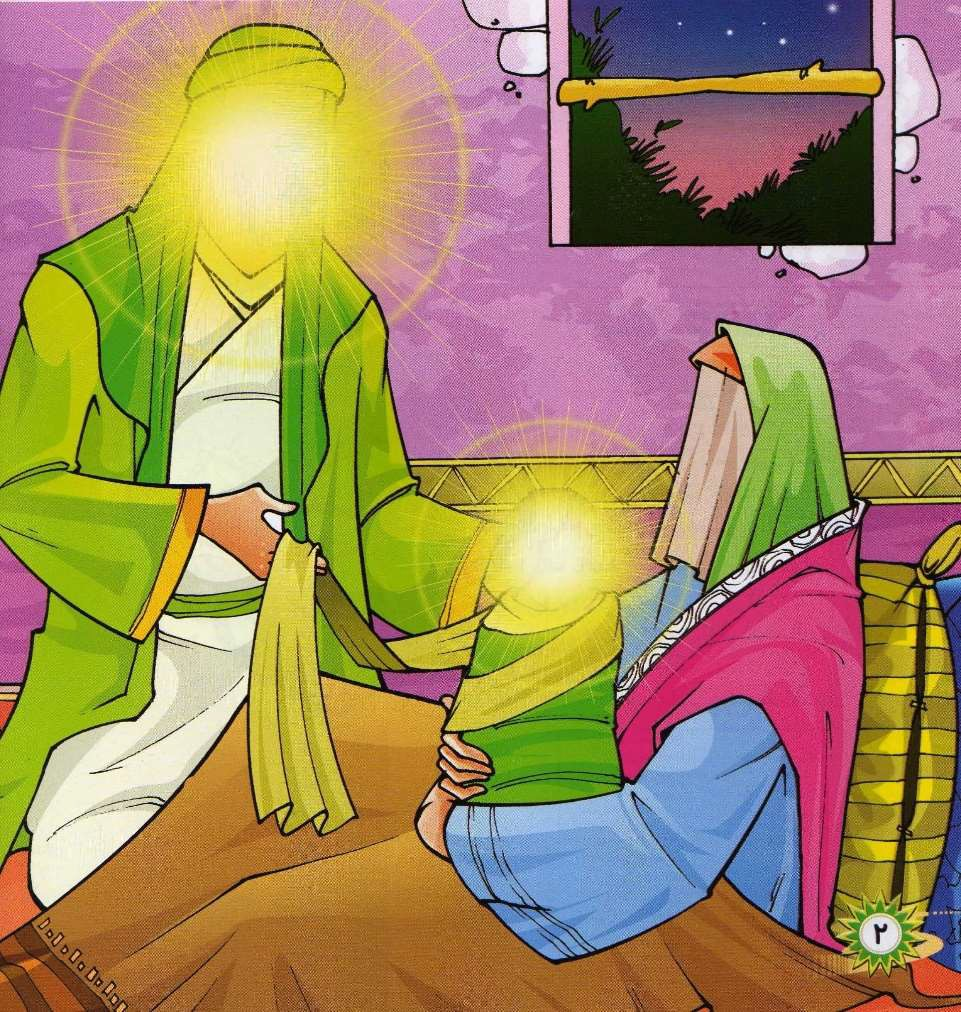
\includegraphics[width=6.3in,height=4.20208in]{media/image4.jpeg}

Selon la théologie musulmane, l'islam est la religion originelle de
l'humanité.VICTOR MOUSSA - STOCK.ADOBE.COM

\subsection{► Que dit la tradition ?}

Selon la théologie musulmane, l'islam est la religion originelle de
l'humanité.~\emph{« Tout homme est né musulman »,}~dit un hadith
attribué
au~\href{https://www.la-croix.com/sacralite-prophete-lislam-2020-11-06-1101123195}{\underline{prophète
Mohammed}}. L'homme est né pour adorer Dieu : certes, il a reçu une
dignité plus haute que les autres créatures, mais celle-ci est
conditionnée à sa soumission au Dieu unique. Plus un homme applique la
loi divine (\emph{charia}), plus il devient humain. Quant au « mécréant
» (\emph{kâfir}), qui refuse de suivre la charia, il se situe en quelque
sorte à un degré inférieur d'humanité.

Cette sévérité envers les non-musulmans s'appuie sur la lecture du texte
coranique qui s'est imposée à partir du IX\textsuperscript{e}~siècle,
lors de la transformation de l'islam en un empire soucieux de se
légitimer. Confortée par des hadiths rédigés à cette époque, elle
dépeint une vérité unique et non négociable. Elle insiste sur les
versets du Coran particulièrement virulents envers les polythéistes,
païens ou idolâtres, qualifiés d'\emph{« associateurs
»}~(\emph{mouchrikoun}) car ils « associent » à Dieu d'autres divinités.

Quant aux athées,~\emph{« ils appartiennent, selon la théologie
musulmane, à une catégorie de mécréance encore inférieure aux
polythéistes, aux juifs et aux chrétiens »,~}explique l'islamologue
Abdessamad Belhaj, chercheur au Centre interdisciplinaire d'études de
l'islam dans le monde contemporain de l'Université catholique de
Louvain. Même si des institutions comme le Haut Conseil des oulémas du
Maroc ou la Maison de la fatwa en Égypte considèrent que les apostats ne
peuvent plus être condamnés à mort, cette peine reste appliquée dans une
dizaine de pays, comme l'Afghanistan ou
la~\href{https://www.la-croix.com/Monde/Afrique/prisons-Mauritanie-calvaire-dun-apostat-2019-09-30-1201051050}{\underline{Mauritanie}}.

\subsection{ Pourquoi juifs et chrétiens bénéficient-ils d'un statut
spécifique ?}

Selon la tradition musulmane, chrétiens et juifs font l'objet d'un
traitement différent des autres non-musulmans : ils bénéficient dans le
droit islamique d'une protection juridique particulière (\emph{dhimma})
toutefois accompagnée d'injonctions humiliantes, comme l'interdiction de
monter à cheval ou de construire des lieux de culte dépassant ceux des
musulmans.
 

\emph{« Le Coran est très ambivalent au sujet des ``gens du Livre''
»,~}rappelle
l'historien~\href{https://www.la-croix.com/Culture/Livres-et-idees/historiens-decryptent-Coran-avant-lislam-2019-11-27-1201063090}{\underline{Guillaume
Dye}}, professeur à l'Université libre de Bruxelles (1). Selon la
sourate 5, juifs et chrétiens ne doivent pas être pris pour~\emph{«
alliés »~}(5, 51) mais, quelques versets plus loin, on lit qu'ils ne
seront~\emph{« point affligés »~}(5, 69). Les chrétiens se voient
reprocher de nier l'unicité de Dieu mais du respect est exprimé pour les
prêtres et les moines, qui~\emph{« ne s'enflent pas d'orgueil ».}

Selon une théologie dite de la falsification (\emph{tahrif}), les juifs
et les chrétiens ont altéré le message transmis par leurs prophètes
respectifs (Moïse, Jésus), message qui n'était autre que l'islam. Le
Coran, lui, corrige cette déviation en transmettant fidèlement le
message révélé à un ultime prophète, Mohammed. À Médine, celui-ci aurait
signé une~\emph{« Constitution »~}disposant que les juifs, notamment,
pouvaient pratiquer leur religion en sécurité, mais ces relations se
sont rapidement détériorées.

\subsection{► Quelles pistes pour une « théologie du pluralisme » ?}

Les attentats visant des « mécréants » en terrasse à Paris, les
persécutions contre les Yézidis ou les chrétiens en Irak, sont autant de
conséquences d'une lecture littéraliste du Coran encouragée par l'essor
du salafisme saoudien à partir des années 1970. D'autres lectures ont
pourtant existé dès les premiers siècles de l'islam. Contrairement à la
doctrine sunnite traditionnelle, l'exégèse rationaliste a par exemple
conclu très tôt à une~\emph{« égalité entre tous les êtres humains, tous
étant dotés de la même raison les rendant aptes à comprendre la parole
de Dieu »,~}rappelle l'islamologue Pierre Lory, directeur d'études à
l'École pratique des hautes études (EPHE).

Pour Abdessamad Belhaj, tout l'enjeu est aujourd'hui de refonder le
rapport à l'altérité sur la base de l'éthique, et de\emph{~« mettre
l'homme au cœur de la théologie »}. Pour cela, certaines valeurs
présentes dans l'islam gagneraient à être redécouvertes, comme celles du
soin, du don et du service à l'humanité, longtemps éclipsées selon lui
par l'autorité et la loyauté à la communauté musulmane ou à la tribu.

(1) Il a codirigé avec Mohammad Ali Amir-Moezzi, Le Coran des
historiens, 2019, Éd. du Cerf, 3~408~p., 89~€.

Faudra-t-il sauver les salafistes ?

Le gouvernement français a voulu lancer en octobre 2019 une offensive
contre l'islamisme et les courants radicaux, rapidement relayée par un
emballement médiatique qui a échappé à tout contrôle. Or, l'ennemi
désigné n'a nullement été identifié selon des termes juridiques, pas
plus que ses torts. On lui reproche sa piété rigoureuse, son voile, sa
pratique du jeûne de Ramadan, sa barbe fournie, son refus de toucher les
femmes, ce qui le rapproche dangereusement de n'importe quel fidèle
conservateur.

L'offensive vise donc une manière de concevoir la piété musulmane, et
nullement une qualification criminelle ou une atteinte à l'ordre public.
C'est dire que nous sommes confrontés à un « délit de sale gueule »,
lequel échappe à la tradition juridique républicaine, délit qui est
indiscernable, sans limite, extensible, mais politiquement pratique
auprès d'une opinion chauffée à blanc par les attentats et
l'immigration.

\subsection{Un engagement d'abord religieux}

Si l'islamiste ainsi décrit ressemble évidemment
au~\href{https://www.la-croix.com/Religion/Islam/Quest-salafisme-2018-10-14-1200975866}{\underline{salafiste}},
c'est oublier un peu vite que l'écrasante majorité des~\emph{salafi~}--
ceux qui sont attachés au modèle des « anciens » (les~\emph{salaf}),
c'est-à-dire les compagnons du Prophète -- se veulent quiétistes : leur
mode d'action est la prédication et l'action missionnaire
(la~\emph{da`wa}). Le salafiste souhaite d'abord vivre un islam épuré et
intégriste -- au sens d'intégral -- dans le cadre de sa famille et de sa
communauté.

Ce mouvement est distinct d'un engagement politique, de sorte que les
salafistes sont rarement liés aux Frères musulmans, qui eux forment un
mouvement politique. Si la matrice religieuse et idéologique du
salafisme imprègne les mentalités djihadistes, elle ne se confond pas
avec celles-ci, ni dans la pensée, ni dans les faits. La radicalisation
concerne donc à des degrés différents et sous des formes incomparables
les sympathisants du salafisme et les partisans du djihadisme de Daech.
Les premiers ont un engagement d'abord religieux, tandis que les autres
sont mus à la fois par la volonté de puissance, des facteurs politiques,
sociaux et religieux.

\subsection{L'autodidacte de l'islam présente plus de risques que le
salafiste}

L'hostilité des salafistes envers les courants djihadistes a été prouvée
à de nombreuses reprises par des déclarations publiques et surtout en
fournissant du renseignement de qualité auprès des services de police.
Le meilleur ennemi du terroriste est souvent le~\emph{salafi}, et
l'autodidacte de l'islam présente plus de risques que le salafiste.

En outre, le salafisme n'a pas été désavoué par les représentants du
culte musulman pour la simple raison que ce courant n'est pas une
idéologie : il faudrait donc lui enlever son~\emph{isme}~final et
l'appeler, selon la tradition religieuse, la~\emph{salafiya~}; il s'agit
d'un vieux courant légitime de l'islam, qui a fourni des générations
d'imams et de lettrés attachés au sens littéral du Coran et de la Sunna.

\subsection{Un « écosystème » étroit mais rassurant}

Il est évident que le salafisme représente une alternative culturelle et
sociale au modèle français, modèle égalitaire, inclusif, ouvert (au
moins en théorie). Les quelques salafi que j'ai connus -- des convertis
à 25 ou 30 \% d'entre eux -- vivaient dans un étroit triangle
géographique. Parce qu'ils souhaitent faire les cinq prières à leur
heure, sans les décaler, et ce dans une salle de prière, ils sont
contraints de vivre et de travailler non loin d'une mosquée. Ils passent
ainsi de leur habitation au lieu de travail et à la salle de prière,
lesquels se situent nécessairement dans un « écosystème » étroit mais
rassurant. Ils ne peuvent guère être exigeants sur le plan
professionnel.

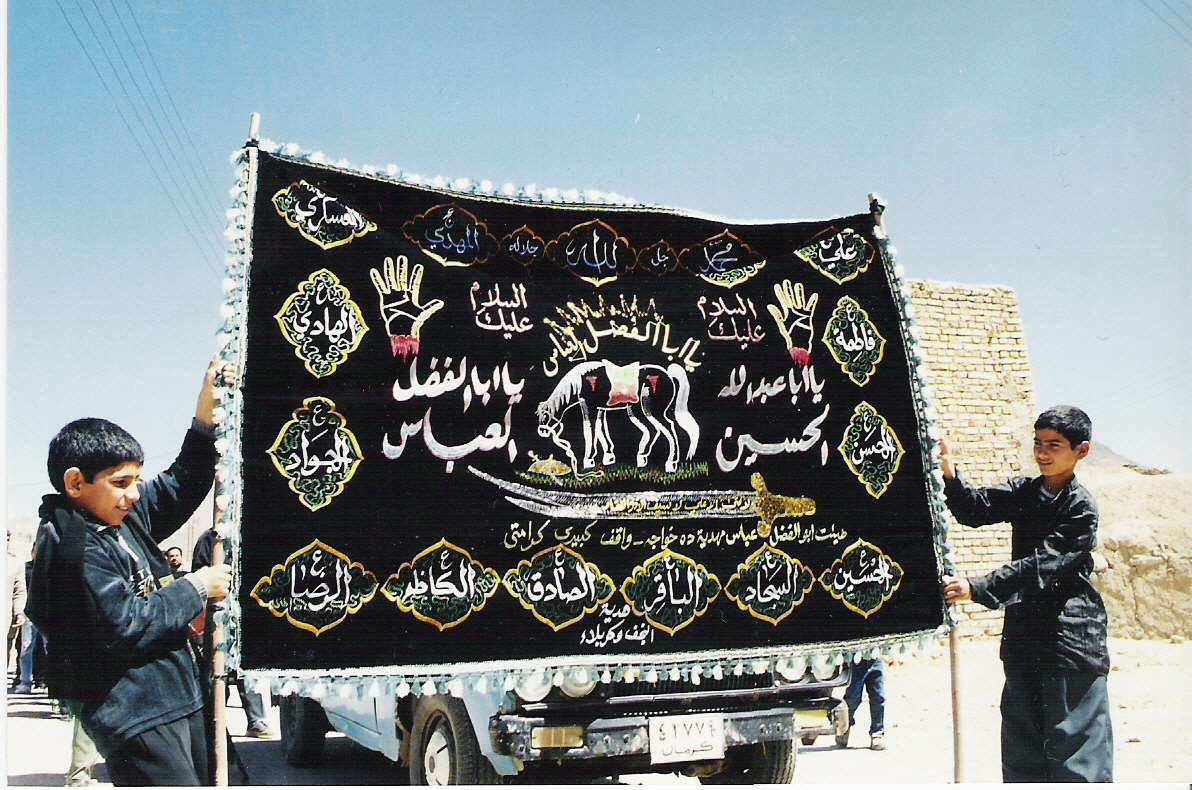
\includegraphics[width=1.97917in,height=1.40972in]{media/image6.jpeg}

\href{https://www.la-croix.com/Religion/Le-Coran-peut-etre-interprete-2021-01-25-1201136852}{Le
Coran peut-il être interprété ?}

Le salafisme, qui représente au moins 40 000 individus, est socialement
dangereux car il impose l'auto-ségrégation, le refus des contacts avec «
ceux qui n'en sont pas ». C'est la raison pour laquelle les spécialistes
des questions de sécurité se refusent à les impliquer dans la lutte
contre le djihadisme. Salafistes et terroristes participeraient à une
même matrice intellectuelle, celle du bien contre le mal, une sorte de
vision sectaire du monde. La différence vient du rapport à la violence :
assumé chez les djihadistes, rejeté chez les salafistes. Leur
fondamentalisme présente l'avantage d'une certaine forme de morale : à
Sartrouville les quartiers salafisés ont vu s'effondrer la toxicomanie
et la délinquance, avec le soutien de la mairie.

\subsection{Confondre l'approche culturelle avec la lutte contre le
terrorisme}

Ces courants ne peuvent être incriminés sur le plan sécuritaire. On
confond donc l'approche culturelle avec la lutte contre le terrorisme. À
moins de changer tout le droit européen, la première doit être menée par
l'éducation, la philosophie, la raison, le débat ; quant à la seconde
elle doit s'appuyer sur le droit et sur des qualifications pénales, et
non sur de vagues impressions de « radicalisation », notion qui n'a
toujours pas été appréhendée de façon rigoureuse en termes sociologiques
et psychologiques.

Comme la guerre d'Algérie nous l'enseigne, une telle manière de
concevoir l'action politique va aboutir à l'effet inverse de celui
recherché : le renforcement de la méfiance collective, le repli
communautaire du côté musulman, l'action violente du côté des « anti »,
et, finalement, la fragmentation sociale et l'insécurité.

\subsection{Islam : les fumées de la radicalisation}

Olivier Hanne, médiéviste (université de Poitiers), chercheur en
islamologie, estime qu'il est très difficile de définir le parcours type
d'une personne radicalisée. Le dernier de trois articles consacrés à
l'islam en France. 
 

Qui parle d'islam aujourd'hui pense aussitôt à la radicalisation. En
2015, on estimait entre 8 000 et 10 000 le nombre de Français
radicalisés. Leurs profils sont si variés qu'il est difficile de donner
des catégories fixes : les mineurs représentent 25 \% des cas, les
femmes 27 \%, les personnes signalées sont plutôt jeunes (entre 16 et 30
ans), leur niveau scolaire est généralement faible, même si l'on
rencontre des diplômés.

La plupart travaillent. Internet représente pour tous ces individus un
passage obligé, même s'il se concrétise différemment : terrain initial
de la radicalisation, facteur de renforcement ou vecteur unique de
l'expression radicale, le partage des contenus djihadistes sur Internet
n'a pas du tout la même fonction chez une adolescente connectée, un
salafiste convaincu et un combattant expérimenté déjà parti en Syrie.

\subsection{Les autorités font feu de tout bois}

De toute évidence, l'attraction pour la radicalité religieuse n'est pas
nécessairement liée à un phénomène de rupture sociale. Les failles de la
société contemporaine (éclatement des familles, déclin des autorités et
des idéologies, chômage, ghettoïsation) créent un terreau facilitateur,
mais nullement déterminant. La frustration individuelle alimente le
recours à des convictions extrêmes, voire le passage à l'acte
terroriste, mais n'est qu'un facteur parmi tant d'autres.

Les autorités font feu de tout bois pour tenter de faire face à une
radicalisation multiforme. En avril 2015, le premier ministre français,
Manuel Valls, annonçait l'ouverture d'une dizaine de centres de
prévention de la radicalisation, dont la plupart furent un échec. Des
sites Internet officiels sont créés et proposent des fiches techniques
contre la radicalisation et le terrorisme, dont le contenu est souvent
simple, voire binaire. Ainsi sur le site
français~\emph{stop-djihadisme.gouv.fr}, un bandeau intitulé «
Radicalisation djihadiste, les premiers signes qui peuvent alerter »
énonce pêle-mêle : « ils se méfient des anciens amis qu'ils considèrent
maintenant comme des impurs » ; « ils changent brutalement leurs
habitudes alimentaires » ; « ils arrêtent d'écouter de la musique car
elle les détourne de leur mission » ; « ils ne regardent plus la
télévision et ne vont plus au cinéma ». Autant de signes extérieurs qui
se rapprochent de l'adolescente anorexique\ldots{} L'efficacité de ces
dispositifs a d'ailleurs été très contestée dès 2015.

\subsection{L'État, tenté d'être omniprésent}

Toute l'entreprise de déradicalisation définit en creux le modèle
positif occidental : monde de loisirs, de consommation, d'épanouissement
personnel et professionnel. Le vocabulaire de la radicalisation masque
le rejet de ce modèle culturel. Et les pouvoirs publics d'hésiter à
appeler leur objectif par son vrai nom : le reconditionnement mental.

Le danger de la déradicalisation se situe dans l'élargissement des
intrusions de l'État : en voulant réinsérer, l'État pénètre dans
l'intimité des individus afin de redéfinir le religieux et lui redonner
une place acceptable. Or, l'État a-t-il compétence pour définir ce
qu'est l'islam, le « bon » islam ? Ne sachant cerner la menace, l'État
est tenté d'être omniprésent, sans en avoir la capacité légale. La
déradicalisation pourrait relever de la posture intellectuelle.

Le problème vient sans doute des hésitations du vocabulaire. Car,
après-tout, qu'est-ce que la radicalisation ? Au
XIX\textsuperscript{e}~le mot anglais~\emph{radical}~était employé pour
désigner les partis politiques britanniques exigeant une réforme
démocratique libérale. Transféré tel quel en France, on l'appliqua aux
partis de gauche, laïques et libéraux qui voulaient réformer la société.

\subsection{Réactions épidermiques}

Le verbe « radicaliser » fut employé régulièrement dans les années
1960-1970 dans une acception politique avec l'idée de « devenir plus
intransigeant, se durcir » ou « plus extrême ». Le premier sens était
donc politique et pas nécessairement négatif. Se déradicaliser était un
synonyme pour « se compromettre ». Appliqué à l'islamisme, le verbe
impose une redéfinition complète des termes : à partir de quand
juge-t-on l'islam intransigeant ou extrême ? par rapport à quelle norme
? à quelle moyenne ?

Les réactions épidermiques qui ont suivi le meurtre de l'enseignant de
Conflans-Sainte-Honorine en octobre 2020 sont tristement révélatrices :
les imams doivent s'exprimer ! les musulmans doivent désavouer le
terrorisme et faire allégeance à la France ! Mais quand ils le font,
c'est encore insuffisant, déloyal et mensonger. Le gouvernement proposa
même qu'ils prient pour la République au cours de la prière collective
du vendredi. Nos références sur la question religieuse restent
tragiquement celles de la Révolution française : comme il y eut les «
prêtres jureurs », adhérant à la loi, contre les « prêtres réfractaires
», obstinés dans leur obéissance à Rome, de la même façon il nous faut
des « imams jureurs », intimement républicains. L'État se retrouve donc
juge des reins et des cœurs.

\chapter{Introduction}
\mn{Christologie, Culture dans l'Histoire - Père Xavier Gué 2022}


\paragraph{Contexte de post modernité}
\begin{Def}[Post modernité]
Une vision du monde déstructurée devant la perte de grand récit fondant le grand récit
\end{Def}

\mn{J.F. Lyotard. Ex : grand récit d'émancipation des lumières}





\backmatter

%\bibliography{Theo}
%\bibliographystyle{siam}
\printbibliography

\listoftheorems[ignoreall,show={Def}]

%\listoftheorems


\end{document}